\section{Beam Line and Detectors}
\label{hptpcPaper:sec:Methods}

    \subsection{Beam Test Overview}
    The beam test took place in the 0.8~GeV T10 beam line, East Area at the Proton Synchrotron in CERN from the 15th August to the 18th September 2018.
    The results in this paper use data taken on the 31st August and 1st September, during which the setup configuration was varied as described below.
    The primary components of the  experimental setup for the data taking period is shown in Figure~\ref{fig:setup}.
    \begin{figure}
    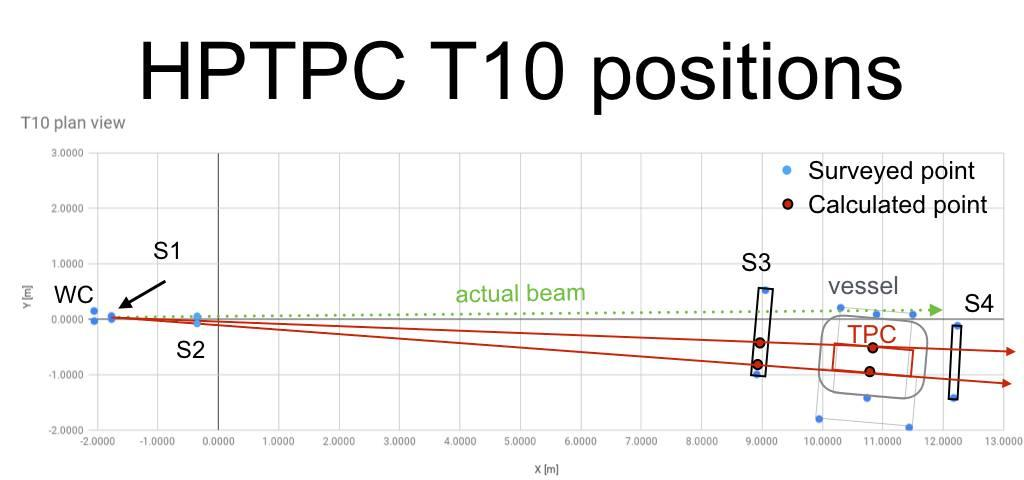
\includegraphics[width=1.0\linewidth]{files/Figures/T10Diagram.jpg}
    	\caption{Beam test configuration}
    		\label{fig:setup}
    \end{figure}
    The centre of the HPTPC Prototype was placed 13~m from the wire chamber at the beam entrance. Three ToF constituents, labeled S1 to S3, were placed upstream of the TPC, while the fourth, labeled S4, was placed directly downstream. Both the TPC and ToF systems were placed at an off-axis angle with respect to the direction of the beam.
    Additionally, a variable number of blocks of acrylic moderator, shown in Figure~\ref{fig:modblocks}, were placed in the beamline, upstream of S1.
      \begin{figure}
      \centering
    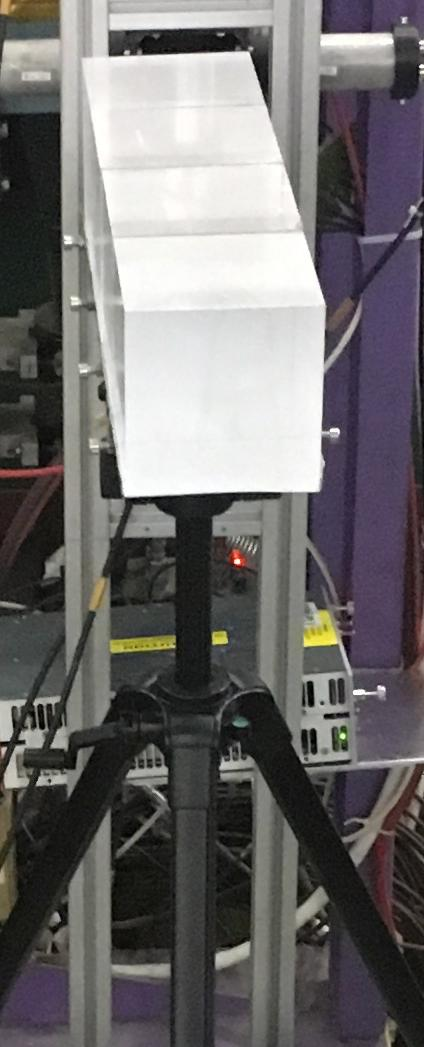
\includegraphics[width=0.2\linewidth]{files/Figures/ModeratorBlocks.jpg}
    	\caption{Acrylic Moderator Blocks}
    		\label{fig:modblocks}
    \end{figure}
    
    A system of moderator blocks was located between the beam wire chambers and ToF constituent S1.  The system is composed of a stand on which up to four polystyrene AxBxC cm blocks can be placed. Figure~\ref{fig:modblocks} shows the stand with four blocks on it. The moderator blocks have the effect of both reducing the energy of incoming particles as well as scattering protons at higher angles than minimum ionizing particles, thus increasing the proton to MIP ratio at off-axis angles from the beam. 
    
    Data was taken with the beam primarily at 0.8~GeV, and with each configuration of 0 to 4 moderator blocks. Figure~INSERT shows the typical composition of the beam upstream of S1 at 0.8~GeV. Beam spills are approximately 500~ms in length with 5-10~s between spills.  
    
%    Moderator blocks were used in order to cause a spread in the incoming beam.
%    The blocks cause protons to scatter through a larger angle than pions and other minimum ionising particles (MIP), increasing the off-axis proton pion ratio.
%    The effect of this, together with placing the TPC and ToF systems off axis was to allow a measurement of protons with a lower pion background.
%    This technique also had the effect of reducing the average momentum of the measured particles.
%    Data were taken for 0, 1, 2, 3, and 4 moderator blocks in turn.
%    The beam ran with an energy of 0.8~GeV, and primarily comprised protons and pions, as well as muons and electrons. 
%    Beam spills were approximately 500~ms in length, with 5-10~s between spills.
%    The ratio of protons to pions expected in the T10 beam  is shown in figure~\ref{beamcharacteristics}.
%    From this figure, the expected on axis proton pion ratio at 0.8~GeV is approximately 1:6.
%      \begin{figure}
%      \centering
%    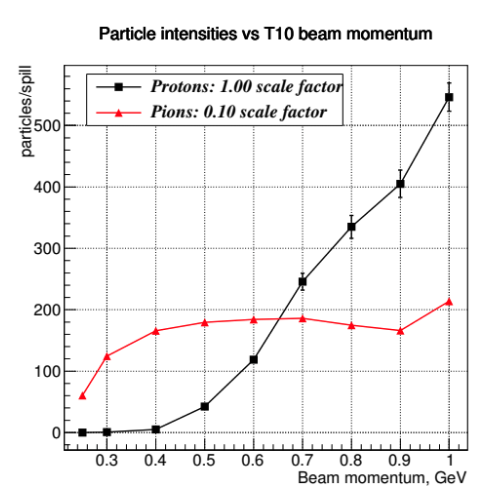
\includegraphics[width=0.6\linewidth]{files/Figures/offaxismeasurement.png}
%    	\caption{T10 beam constituents (REFERENCE NEEDED)}
%    		\label{fig:beamcharacteristics}
%    \end{figure}
    
    
	\subsection{Upstream beam counters S1 and S2}
	
	S1 and S2 are shown in Figure~\ref{fig:WHAT}. S1 is a $40\times40\times5$~mm$^3$ plastic scintillator tile which is attached to four 1'' Hamamatsu R4998 phototubes from four ends for the light readout. The time resolution of the counter, as measured by the DAQ system of the upstream ToF, was about 30 ps. 
	
	S2 was placed 1~m downstream of S1. The size of the scintillator tile, $120\times120\times5$~mm$^3$, was adjusted to account for the beam divergence in the moderator blocks. The light was collected by a 2'' PMT R13089 which was connected to the scintillator via long light-guide as shown in Figure~\ref{fig:WHAT}. 
	
	The analog signals from one of the S1 PMTs (WHICH ONE??) and S2 PMT were fed into discriminator units set at AA mV and BB mV respectively. These two signals were fed into a coincidence unit, and the coincidence of the two signals was used by the S3 and S4 ToF constituents for time-of-flight analyses. 

    
\subsection{Upstream Time of Flight instrumentation (S3)}

The S3 `upstream' ToF constituent sits just upstream of the HPTPC prototype in the beamline. The sketch of the S3 ToF constituent is shown in Figure~\ref{fig:S3sketch}. The detector is composed of 22 staggered bars:  20 bars with dimensions $1.68 \times 6 \times 1$~cm$^3$ and 2 bars of  $1.5 \times 6 \times 1$~cm$^3$ placed on top and bottom.
The overlap between bars was set to 5~mm, thus the active area of the detector was approximately 1.68 m $\times$ 1.22 m.
     \begin{figure}
      \centering
    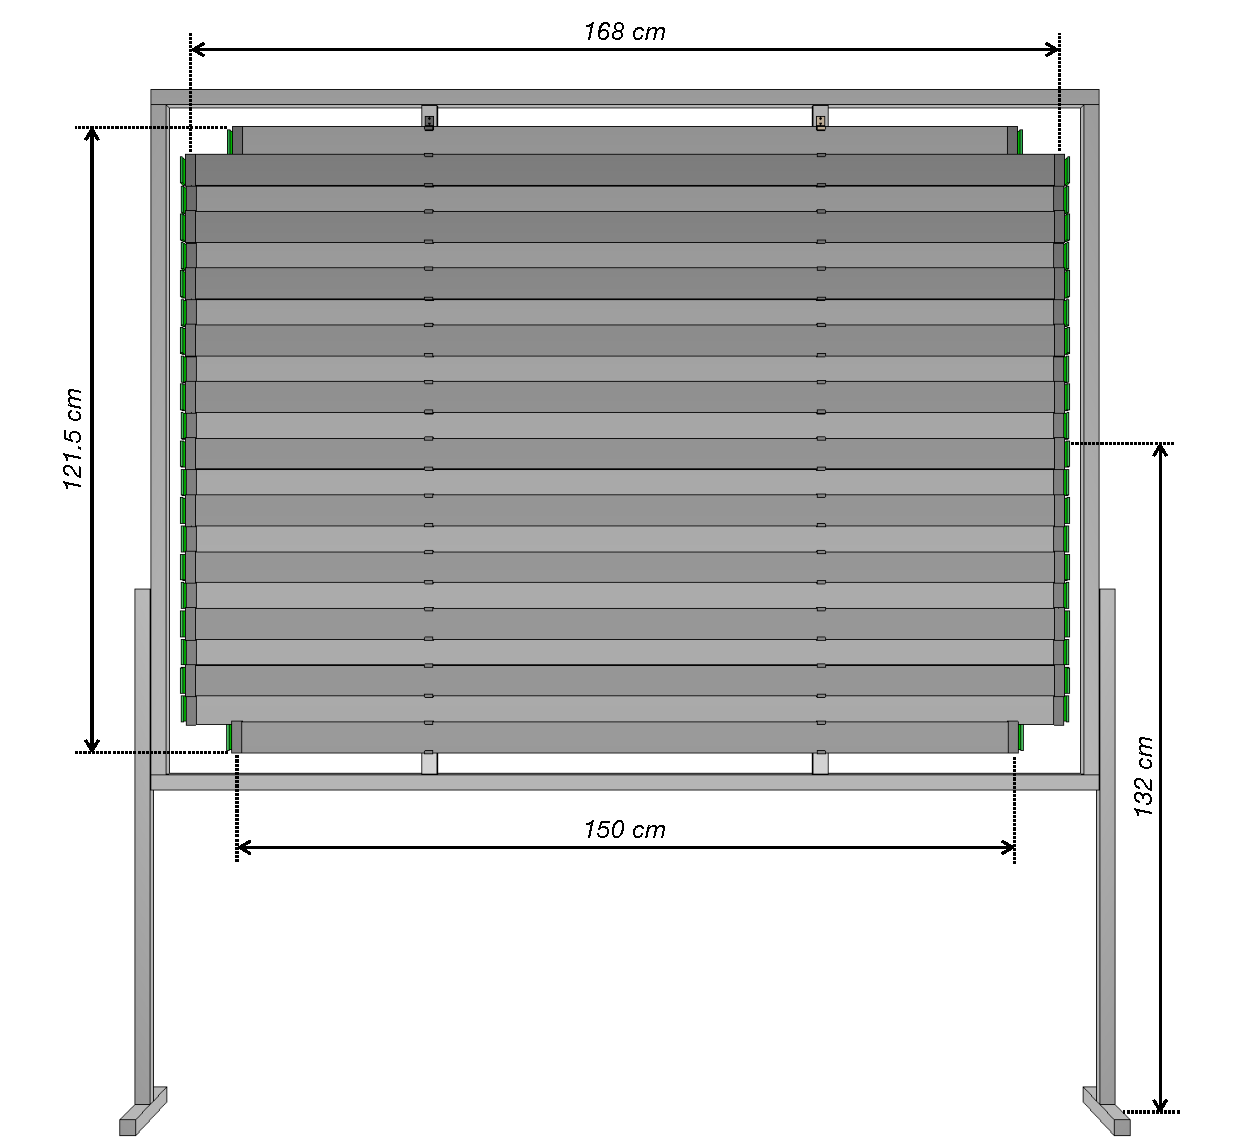
\includegraphics[width=0.7\linewidth]{files/Figures/uToF_sketch.pdf}
    	\caption{Sketch of the S3 wall}
    		\label{fig:S3sketch}
    \end{figure}
    
The bars are made from the plastic EJ-200, which provides a suitable optical attenuation length 4~m and fast timing (rise time of 0.9~ns and decay time 2.1~ns) REFERENCE?. The scintillation emission spectrum of EJ-200 is primarily in the violet region of the visible spectrum. REFERENCE?

Arrays of eight $6 \times 6$~mm$^2$ area silicone photomultipliers (SiPMs) from Hamamatsu Photonics were coupled to both ends of the bar to collect scintillation photons. Anode signals of SiPMs have been read out and summed by an 8-channel SiPM anode readout integrated circuit MUSIC-R1. %The construction of the prototype was a joint effort between groups of Geneva and Zurich universities as a part of R\&D for the Timing detector of the SHIP experiment \cite{AK}.

A 64-ch SAMPIC  module was used for the data acquisition. A SAMPIC chip is a Waveform and Time to Digital Converter (WTDC) multichannel ASIC which provides a raw time with an ultrafast analog memory allowing fine timing extraction as well as other parameters of the pulse \cite{SAMPIC}. Each channel integrates a discriminator that can trigger itself independently or participate to a more complex trigger. 

A mean time of light signals detected at two ends of a single bar provides a time reference with the resolution of about 100 ps, while the time difference gives a position of the interaction along the bar, with a resolution of NNN. Examples of reconstructed $XY$ distributions are shown in Figures~\ref{fig:s3XY_pion} and~\ref{fig:s3XY_proton}.

\begin{figure}[ht]
	\begin{minipage}[t]{0.49\textwidth}
		\centering
		\begin{adjustbox}{max totalsize={\textwidth}{.5\textheight},center}
			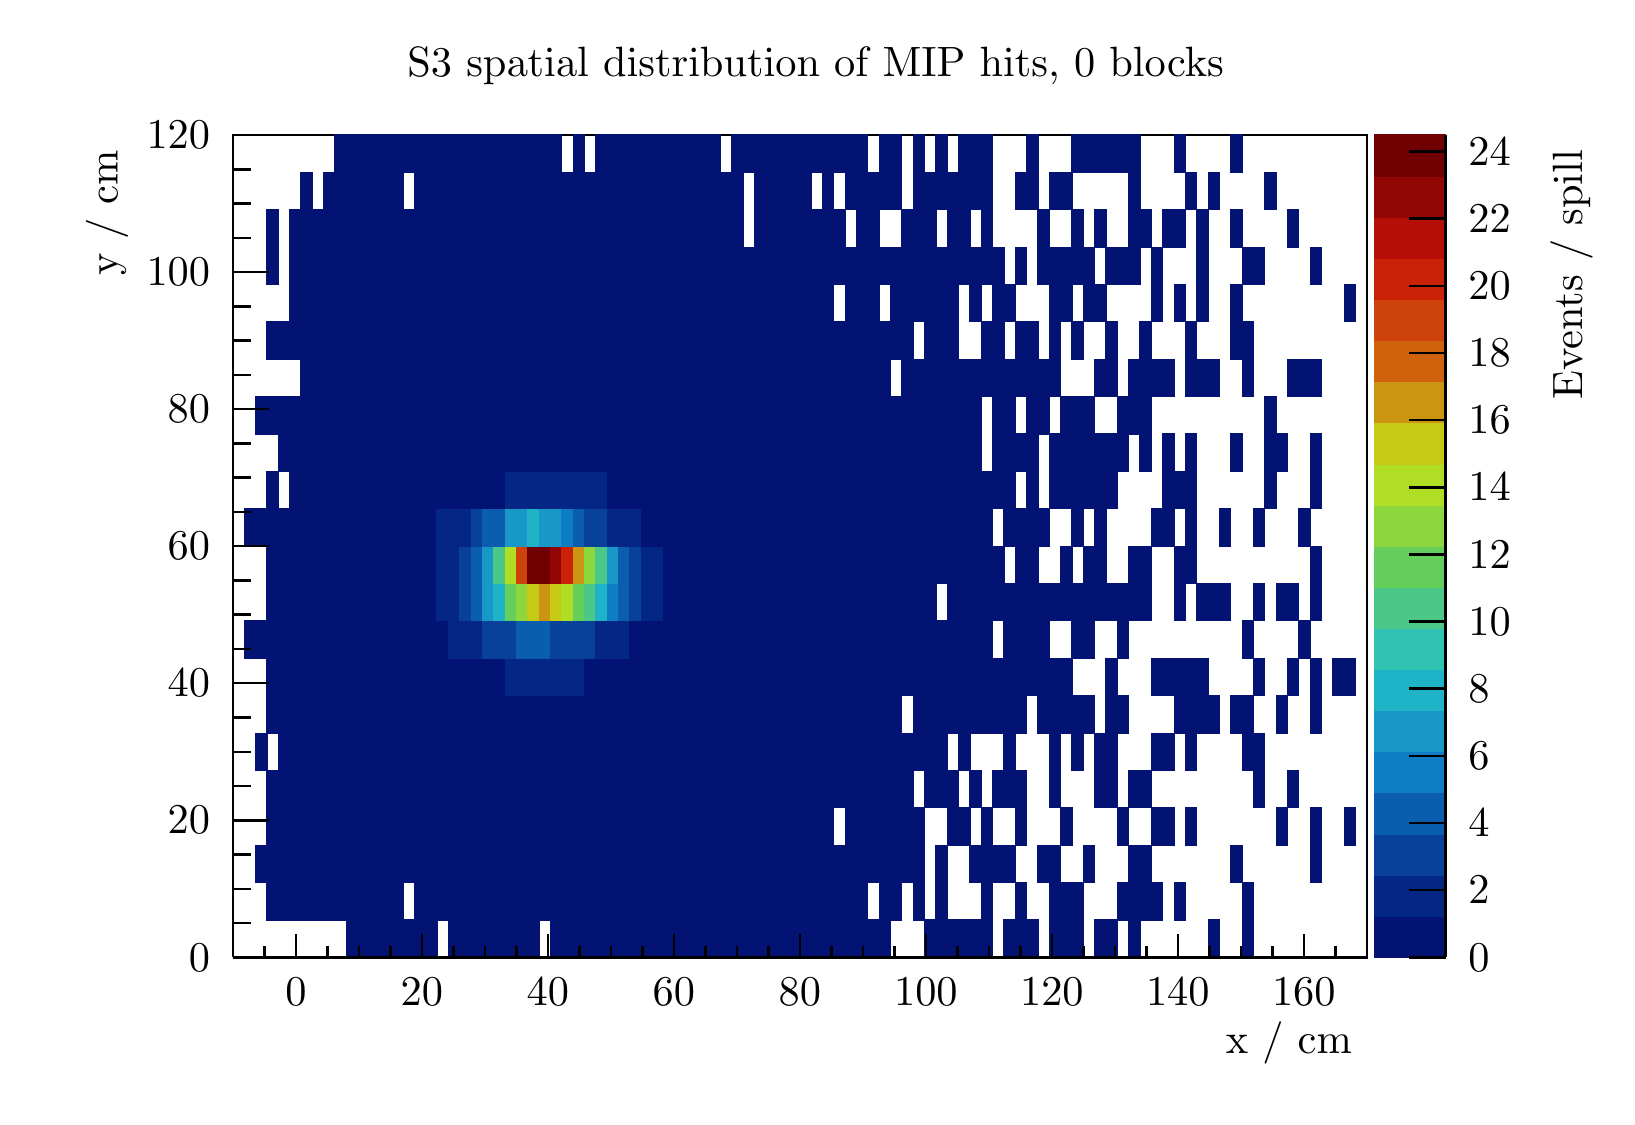
\begin{tikzpicture}
\pgfdeclareplotmark{cross} {
\pgfpathmoveto{\pgfpoint{-0.3\pgfplotmarksize}{\pgfplotmarksize}}
\pgfpathlineto{\pgfpoint{+0.3\pgfplotmarksize}{\pgfplotmarksize}}
\pgfpathlineto{\pgfpoint{+0.3\pgfplotmarksize}{0.3\pgfplotmarksize}}
\pgfpathlineto{\pgfpoint{+1\pgfplotmarksize}{0.3\pgfplotmarksize}}
\pgfpathlineto{\pgfpoint{+1\pgfplotmarksize}{-0.3\pgfplotmarksize}}
\pgfpathlineto{\pgfpoint{+0.3\pgfplotmarksize}{-0.3\pgfplotmarksize}}
\pgfpathlineto{\pgfpoint{+0.3\pgfplotmarksize}{-1.\pgfplotmarksize}}
\pgfpathlineto{\pgfpoint{-0.3\pgfplotmarksize}{-1.\pgfplotmarksize}}
\pgfpathlineto{\pgfpoint{-0.3\pgfplotmarksize}{-0.3\pgfplotmarksize}}
\pgfpathlineto{\pgfpoint{-1.\pgfplotmarksize}{-0.3\pgfplotmarksize}}
\pgfpathlineto{\pgfpoint{-1.\pgfplotmarksize}{0.3\pgfplotmarksize}}
\pgfpathlineto{\pgfpoint{-0.3\pgfplotmarksize}{0.3\pgfplotmarksize}}
\pgfpathclose
\pgfusepathqstroke
}
\pgfdeclareplotmark{cross*} {
\pgfpathmoveto{\pgfpoint{-0.3\pgfplotmarksize}{\pgfplotmarksize}}
\pgfpathlineto{\pgfpoint{+0.3\pgfplotmarksize}{\pgfplotmarksize}}
\pgfpathlineto{\pgfpoint{+0.3\pgfplotmarksize}{0.3\pgfplotmarksize}}
\pgfpathlineto{\pgfpoint{+1\pgfplotmarksize}{0.3\pgfplotmarksize}}
\pgfpathlineto{\pgfpoint{+1\pgfplotmarksize}{-0.3\pgfplotmarksize}}
\pgfpathlineto{\pgfpoint{+0.3\pgfplotmarksize}{-0.3\pgfplotmarksize}}
\pgfpathlineto{\pgfpoint{+0.3\pgfplotmarksize}{-1.\pgfplotmarksize}}
\pgfpathlineto{\pgfpoint{-0.3\pgfplotmarksize}{-1.\pgfplotmarksize}}
\pgfpathlineto{\pgfpoint{-0.3\pgfplotmarksize}{-0.3\pgfplotmarksize}}
\pgfpathlineto{\pgfpoint{-1.\pgfplotmarksize}{-0.3\pgfplotmarksize}}
\pgfpathlineto{\pgfpoint{-1.\pgfplotmarksize}{0.3\pgfplotmarksize}}
\pgfpathlineto{\pgfpoint{-0.3\pgfplotmarksize}{0.3\pgfplotmarksize}}
\pgfpathclose
\pgfusepathqfillstroke
}
\pgfdeclareplotmark{newstar} {
\pgfpathmoveto{\pgfqpoint{0pt}{\pgfplotmarksize}}
\pgfpathlineto{\pgfqpointpolar{44}{0.5\pgfplotmarksize}}
\pgfpathlineto{\pgfqpointpolar{18}{\pgfplotmarksize}}
\pgfpathlineto{\pgfqpointpolar{-20}{0.5\pgfplotmarksize}}
\pgfpathlineto{\pgfqpointpolar{-54}{\pgfplotmarksize}}
\pgfpathlineto{\pgfqpointpolar{-90}{0.5\pgfplotmarksize}}
\pgfpathlineto{\pgfqpointpolar{234}{\pgfplotmarksize}}
\pgfpathlineto{\pgfqpointpolar{198}{0.5\pgfplotmarksize}}
\pgfpathlineto{\pgfqpointpolar{162}{\pgfplotmarksize}}
\pgfpathlineto{\pgfqpointpolar{134}{0.5\pgfplotmarksize}}
\pgfpathclose
\pgfusepathqstroke
}
\pgfdeclareplotmark{newstar*} {
\pgfpathmoveto{\pgfqpoint{0pt}{\pgfplotmarksize}}
\pgfpathlineto{\pgfqpointpolar{44}{0.5\pgfplotmarksize}}
\pgfpathlineto{\pgfqpointpolar{18}{\pgfplotmarksize}}
\pgfpathlineto{\pgfqpointpolar{-20}{0.5\pgfplotmarksize}}
\pgfpathlineto{\pgfqpointpolar{-54}{\pgfplotmarksize}}
\pgfpathlineto{\pgfqpointpolar{-90}{0.5\pgfplotmarksize}}
\pgfpathlineto{\pgfqpointpolar{234}{\pgfplotmarksize}}
\pgfpathlineto{\pgfqpointpolar{198}{0.5\pgfplotmarksize}}
\pgfpathlineto{\pgfqpointpolar{162}{\pgfplotmarksize}}
\pgfpathlineto{\pgfqpointpolar{134}{0.5\pgfplotmarksize}}
\pgfpathclose
\pgfusepathqfillstroke
}
\definecolor{c}{rgb}{1,1,1};
\draw [color=c, fill=c] (0,0) rectangle (20,13.5632);
\draw [color=c, fill=c] (2.6,1.76322) rectangle (17,12.2069);
\definecolor{c}{rgb}{0,0,0};
\draw [c,line width=0.9] (2.6,1.76322) -- (2.6,12.2069) -- (17,12.2069) -- (17,1.76322) -- (2.6,1.76322);
\definecolor{c}{rgb}{1,1,1};
\draw [color=c, fill=c] (2.6,1.76322) rectangle (17,12.2069);
\definecolor{c}{rgb}{0,0,0};
\draw [c,line width=0.9] (2.6,1.76322) -- (2.6,12.2069) -- (17,12.2069) -- (17,1.76322) -- (2.6,1.76322);
\definecolor{c}{rgb}{0.00759013,0.0728653,0.45351};
\draw [color=c, fill=c] (4.04,1.76322) rectangle (4.184,2.23793);
\draw [color=c, fill=c] (4.184,1.76322) rectangle (4.328,2.23793);
\draw [color=c, fill=c] (4.328,1.76322) rectangle (4.472,2.23793);
\draw [color=c, fill=c] (4.472,1.76322) rectangle (4.616,2.23793);
\draw [color=c, fill=c] (4.616,1.76322) rectangle (4.76,2.23793);
\draw [color=c, fill=c] (4.76,1.76322) rectangle (4.904,2.23793);
\draw [color=c, fill=c] (4.904,1.76322) rectangle (5.048,2.23793);
\draw [color=c, fill=c] (5.048,1.76322) rectangle (5.192,2.23793);
\draw [color=c, fill=c] (5.336,1.76322) rectangle (5.48,2.23793);
\draw [color=c, fill=c] (5.48,1.76322) rectangle (5.624,2.23793);
\draw [color=c, fill=c] (5.624,1.76322) rectangle (5.768,2.23793);
\draw [color=c, fill=c] (5.768,1.76322) rectangle (5.912,2.23793);
\draw [color=c, fill=c] (5.912,1.76322) rectangle (6.056,2.23793);
\draw [color=c, fill=c] (6.056,1.76322) rectangle (6.2,2.23793);
\draw [color=c, fill=c] (6.2,1.76322) rectangle (6.344,2.23793);
\draw [color=c, fill=c] (6.344,1.76322) rectangle (6.488,2.23793);
\draw [color=c, fill=c] (6.632,1.76322) rectangle (6.776,2.23793);
\draw [color=c, fill=c] (6.776,1.76322) rectangle (6.92,2.23793);
\draw [color=c, fill=c] (6.92,1.76322) rectangle (7.064,2.23793);
\draw [color=c, fill=c] (7.064,1.76322) rectangle (7.208,2.23793);
\draw [color=c, fill=c] (7.208,1.76322) rectangle (7.352,2.23793);
\draw [color=c, fill=c] (7.352,1.76322) rectangle (7.496,2.23793);
\draw [color=c, fill=c] (7.496,1.76322) rectangle (7.64,2.23793);
\draw [color=c, fill=c] (7.64,1.76322) rectangle (7.784,2.23793);
\draw [color=c, fill=c] (7.784,1.76322) rectangle (7.928,2.23793);
\draw [color=c, fill=c] (7.928,1.76322) rectangle (8.072,2.23793);
\draw [color=c, fill=c] (8.072,1.76322) rectangle (8.216,2.23793);
\draw [color=c, fill=c] (8.216,1.76322) rectangle (8.36,2.23793);
\draw [color=c, fill=c] (8.36,1.76322) rectangle (8.504,2.23793);
\draw [color=c, fill=c] (8.504,1.76322) rectangle (8.648,2.23793);
\draw [color=c, fill=c] (8.648,1.76322) rectangle (8.792,2.23793);
\draw [color=c, fill=c] (8.792,1.76322) rectangle (8.936,2.23793);
\draw [color=c, fill=c] (8.936,1.76322) rectangle (9.08,2.23793);
\draw [color=c, fill=c] (9.08,1.76322) rectangle (9.224,2.23793);
\draw [color=c, fill=c] (9.224,1.76322) rectangle (9.368,2.23793);
\draw [color=c, fill=c] (9.368,1.76322) rectangle (9.512,2.23793);
\draw [color=c, fill=c] (9.512,1.76322) rectangle (9.656,2.23793);
\draw [color=c, fill=c] (9.656,1.76322) rectangle (9.8,2.23793);
\draw [color=c, fill=c] (9.8,1.76322) rectangle (9.944,2.23793);
\draw [color=c, fill=c] (9.944,1.76322) rectangle (10.088,2.23793);
\draw [color=c, fill=c] (10.088,1.76322) rectangle (10.232,2.23793);
\draw [color=c, fill=c] (10.232,1.76322) rectangle (10.376,2.23793);
\draw [color=c, fill=c] (10.376,1.76322) rectangle (10.52,2.23793);
\draw [color=c, fill=c] (10.52,1.76322) rectangle (10.664,2.23793);
\draw [color=c, fill=c] (10.664,1.76322) rectangle (10.808,2.23793);
\draw [color=c, fill=c] (10.808,1.76322) rectangle (10.952,2.23793);
\draw [color=c, fill=c] (11.384,1.76322) rectangle (11.528,2.23793);
\draw [color=c, fill=c] (11.528,1.76322) rectangle (11.672,2.23793);
\draw [color=c, fill=c] (11.672,1.76322) rectangle (11.816,2.23793);
\draw [color=c, fill=c] (11.816,1.76322) rectangle (11.96,2.23793);
\draw [color=c, fill=c] (11.96,1.76322) rectangle (12.104,2.23793);
\draw [color=c, fill=c] (12.104,1.76322) rectangle (12.248,2.23793);
\draw [color=c, fill=c] (12.392,1.76322) rectangle (12.536,2.23793);
\draw [color=c, fill=c] (12.536,1.76322) rectangle (12.68,2.23793);
\draw [color=c, fill=c] (12.68,1.76322) rectangle (12.824,2.23793);
\draw [color=c, fill=c] (12.968,1.76322) rectangle (13.112,2.23793);
\draw [color=c, fill=c] (13.112,1.76322) rectangle (13.256,2.23793);
\draw [color=c, fill=c] (13.256,1.76322) rectangle (13.4,2.23793);
\draw [color=c, fill=c] (13.544,1.76322) rectangle (13.688,2.23793);
\draw [color=c, fill=c] (13.688,1.76322) rectangle (13.832,2.23793);
\draw [color=c, fill=c] (13.976,1.76322) rectangle (14.12,2.23793);
\draw [color=c, fill=c] (14.984,1.76322) rectangle (15.128,2.23793);
\draw [color=c, fill=c] (15.416,1.76322) rectangle (15.56,2.23793);
\draw [color=c, fill=c] (3.032,2.23793) rectangle (3.176,2.71264);
\draw [color=c, fill=c] (3.176,2.23793) rectangle (3.32,2.71264);
\draw [color=c, fill=c] (3.32,2.23793) rectangle (3.464,2.71264);
\draw [color=c, fill=c] (3.464,2.23793) rectangle (3.608,2.71264);
\draw [color=c, fill=c] (3.608,2.23793) rectangle (3.752,2.71264);
\draw [color=c, fill=c] (3.752,2.23793) rectangle (3.896,2.71264);
\draw [color=c, fill=c] (3.896,2.23793) rectangle (4.04,2.71264);
\draw [color=c, fill=c] (4.04,2.23793) rectangle (4.184,2.71264);
\draw [color=c, fill=c] (4.184,2.23793) rectangle (4.328,2.71264);
\draw [color=c, fill=c] (4.328,2.23793) rectangle (4.472,2.71264);
\draw [color=c, fill=c] (4.472,2.23793) rectangle (4.616,2.71264);
\draw [color=c, fill=c] (4.616,2.23793) rectangle (4.76,2.71264);
\draw [color=c, fill=c] (4.904,2.23793) rectangle (5.048,2.71264);
\draw [color=c, fill=c] (5.048,2.23793) rectangle (5.192,2.71264);
\draw [color=c, fill=c] (5.192,2.23793) rectangle (5.336,2.71264);
\draw [color=c, fill=c] (5.336,2.23793) rectangle (5.48,2.71264);
\draw [color=c, fill=c] (5.48,2.23793) rectangle (5.624,2.71264);
\draw [color=c, fill=c] (5.624,2.23793) rectangle (5.768,2.71264);
\draw [color=c, fill=c] (5.768,2.23793) rectangle (5.912,2.71264);
\draw [color=c, fill=c] (5.912,2.23793) rectangle (6.056,2.71264);
\draw [color=c, fill=c] (6.056,2.23793) rectangle (6.2,2.71264);
\draw [color=c, fill=c] (6.2,2.23793) rectangle (6.344,2.71264);
\draw [color=c, fill=c] (6.344,2.23793) rectangle (6.488,2.71264);
\draw [color=c, fill=c] (6.488,2.23793) rectangle (6.632,2.71264);
\draw [color=c, fill=c] (6.632,2.23793) rectangle (6.776,2.71264);
\draw [color=c, fill=c] (6.776,2.23793) rectangle (6.92,2.71264);
\draw [color=c, fill=c] (6.92,2.23793) rectangle (7.064,2.71264);
\draw [color=c, fill=c] (7.064,2.23793) rectangle (7.208,2.71264);
\draw [color=c, fill=c] (7.208,2.23793) rectangle (7.352,2.71264);
\draw [color=c, fill=c] (7.352,2.23793) rectangle (7.496,2.71264);
\draw [color=c, fill=c] (7.496,2.23793) rectangle (7.64,2.71264);
\draw [color=c, fill=c] (7.64,2.23793) rectangle (7.784,2.71264);
\draw [color=c, fill=c] (7.784,2.23793) rectangle (7.928,2.71264);
\draw [color=c, fill=c] (7.928,2.23793) rectangle (8.072,2.71264);
\draw [color=c, fill=c] (8.072,2.23793) rectangle (8.216,2.71264);
\draw [color=c, fill=c] (8.216,2.23793) rectangle (8.36,2.71264);
\draw [color=c, fill=c] (8.36,2.23793) rectangle (8.504,2.71264);
\draw [color=c, fill=c] (8.504,2.23793) rectangle (8.648,2.71264);
\draw [color=c, fill=c] (8.648,2.23793) rectangle (8.792,2.71264);
\draw [color=c, fill=c] (8.792,2.23793) rectangle (8.936,2.71264);
\draw [color=c, fill=c] (8.936,2.23793) rectangle (9.08,2.71264);
\draw [color=c, fill=c] (9.08,2.23793) rectangle (9.224,2.71264);
\draw [color=c, fill=c] (9.224,2.23793) rectangle (9.368,2.71264);
\draw [color=c, fill=c] (9.368,2.23793) rectangle (9.512,2.71264);
\draw [color=c, fill=c] (9.512,2.23793) rectangle (9.656,2.71264);
\draw [color=c, fill=c] (9.656,2.23793) rectangle (9.8,2.71264);
\draw [color=c, fill=c] (9.8,2.23793) rectangle (9.944,2.71264);
\draw [color=c, fill=c] (9.944,2.23793) rectangle (10.088,2.71264);
\draw [color=c, fill=c] (10.088,2.23793) rectangle (10.232,2.71264);
\draw [color=c, fill=c] (10.232,2.23793) rectangle (10.376,2.71264);
\draw [color=c, fill=c] (10.376,2.23793) rectangle (10.52,2.71264);
\draw [color=c, fill=c] (10.52,2.23793) rectangle (10.664,2.71264);
\draw [color=c, fill=c] (10.808,2.23793) rectangle (10.952,2.71264);
\draw [color=c, fill=c] (10.952,2.23793) rectangle (11.096,2.71264);
\draw [color=c, fill=c] (11.24,2.23793) rectangle (11.384,2.71264);
\draw [color=c, fill=c] (11.528,2.23793) rectangle (11.672,2.71264);
\draw [color=c, fill=c] (12.104,2.23793) rectangle (12.248,2.71264);
\draw [color=c, fill=c] (12.536,2.23793) rectangle (12.68,2.71264);
\draw [color=c, fill=c] (12.968,2.23793) rectangle (13.112,2.71264);
\draw [color=c, fill=c] (13.112,2.23793) rectangle (13.256,2.71264);
\draw [color=c, fill=c] (13.256,2.23793) rectangle (13.4,2.71264);
\draw [color=c, fill=c] (13.832,2.23793) rectangle (13.976,2.71264);
\draw [color=c, fill=c] (13.976,2.23793) rectangle (14.12,2.71264);
\draw [color=c, fill=c] (14.12,2.23793) rectangle (14.264,2.71264);
\draw [color=c, fill=c] (14.264,2.23793) rectangle (14.408,2.71264);
\draw [color=c, fill=c] (14.552,2.23793) rectangle (14.696,2.71264);
\draw [color=c, fill=c] (15.416,2.23793) rectangle (15.56,2.71264);
\draw [color=c, fill=c] (2.888,2.71264) rectangle (3.032,3.18736);
\draw [color=c, fill=c] (3.032,2.71264) rectangle (3.176,3.18736);
\draw [color=c, fill=c] (3.176,2.71264) rectangle (3.32,3.18736);
\draw [color=c, fill=c] (3.32,2.71264) rectangle (3.464,3.18736);
\draw [color=c, fill=c] (3.464,2.71264) rectangle (3.608,3.18736);
\draw [color=c, fill=c] (3.608,2.71264) rectangle (3.752,3.18736);
\draw [color=c, fill=c] (3.752,2.71264) rectangle (3.896,3.18736);
\draw [color=c, fill=c] (3.896,2.71264) rectangle (4.04,3.18736);
\draw [color=c, fill=c] (4.04,2.71264) rectangle (4.184,3.18736);
\draw [color=c, fill=c] (4.184,2.71264) rectangle (4.328,3.18736);
\draw [color=c, fill=c] (4.328,2.71264) rectangle (4.472,3.18736);
\draw [color=c, fill=c] (4.472,2.71264) rectangle (4.616,3.18736);
\draw [color=c, fill=c] (4.616,2.71264) rectangle (4.76,3.18736);
\draw [color=c, fill=c] (4.76,2.71264) rectangle (4.904,3.18736);
\draw [color=c, fill=c] (4.904,2.71264) rectangle (5.048,3.18736);
\draw [color=c, fill=c] (5.048,2.71264) rectangle (5.192,3.18736);
\draw [color=c, fill=c] (5.192,2.71264) rectangle (5.336,3.18736);
\draw [color=c, fill=c] (5.336,2.71264) rectangle (5.48,3.18736);
\draw [color=c, fill=c] (5.48,2.71264) rectangle (5.624,3.18736);
\draw [color=c, fill=c] (5.624,2.71264) rectangle (5.768,3.18736);
\draw [color=c, fill=c] (5.768,2.71264) rectangle (5.912,3.18736);
\draw [color=c, fill=c] (5.912,2.71264) rectangle (6.056,3.18736);
\draw [color=c, fill=c] (6.056,2.71264) rectangle (6.2,3.18736);
\draw [color=c, fill=c] (6.2,2.71264) rectangle (6.344,3.18736);
\draw [color=c, fill=c] (6.344,2.71264) rectangle (6.488,3.18736);
\draw [color=c, fill=c] (6.488,2.71264) rectangle (6.632,3.18736);
\draw [color=c, fill=c] (6.632,2.71264) rectangle (6.776,3.18736);
\draw [color=c, fill=c] (6.776,2.71264) rectangle (6.92,3.18736);
\draw [color=c, fill=c] (6.92,2.71264) rectangle (7.064,3.18736);
\draw [color=c, fill=c] (7.064,2.71264) rectangle (7.208,3.18736);
\draw [color=c, fill=c] (7.208,2.71264) rectangle (7.352,3.18736);
\draw [color=c, fill=c] (7.352,2.71264) rectangle (7.496,3.18736);
\draw [color=c, fill=c] (7.496,2.71264) rectangle (7.64,3.18736);
\draw [color=c, fill=c] (7.64,2.71264) rectangle (7.784,3.18736);
\draw [color=c, fill=c] (7.784,2.71264) rectangle (7.928,3.18736);
\draw [color=c, fill=c] (7.928,2.71264) rectangle (8.072,3.18736);
\draw [color=c, fill=c] (8.072,2.71264) rectangle (8.216,3.18736);
\draw [color=c, fill=c] (8.216,2.71264) rectangle (8.36,3.18736);
\draw [color=c, fill=c] (8.36,2.71264) rectangle (8.504,3.18736);
\draw [color=c, fill=c] (8.504,2.71264) rectangle (8.648,3.18736);
\draw [color=c, fill=c] (8.648,2.71264) rectangle (8.792,3.18736);
\draw [color=c, fill=c] (8.792,2.71264) rectangle (8.936,3.18736);
\draw [color=c, fill=c] (8.936,2.71264) rectangle (9.08,3.18736);
\draw [color=c, fill=c] (9.08,2.71264) rectangle (9.224,3.18736);
\draw [color=c, fill=c] (9.224,2.71264) rectangle (9.368,3.18736);
\draw [color=c, fill=c] (9.368,2.71264) rectangle (9.512,3.18736);
\draw [color=c, fill=c] (9.512,2.71264) rectangle (9.656,3.18736);
\draw [color=c, fill=c] (9.656,2.71264) rectangle (9.8,3.18736);
\draw [color=c, fill=c] (9.8,2.71264) rectangle (9.944,3.18736);
\draw [color=c, fill=c] (9.944,2.71264) rectangle (10.088,3.18736);
\draw [color=c, fill=c] (10.088,2.71264) rectangle (10.232,3.18736);
\draw [color=c, fill=c] (10.232,2.71264) rectangle (10.376,3.18736);
\draw [color=c, fill=c] (10.376,2.71264) rectangle (10.52,3.18736);
\draw [color=c, fill=c] (10.52,2.71264) rectangle (10.664,3.18736);
\draw [color=c, fill=c] (10.664,2.71264) rectangle (10.808,3.18736);
\draw [color=c, fill=c] (10.808,2.71264) rectangle (10.952,3.18736);
\draw [color=c, fill=c] (10.952,2.71264) rectangle (11.096,3.18736);
\draw [color=c, fill=c] (11.096,2.71264) rectangle (11.24,3.18736);
\draw [color=c, fill=c] (11.24,2.71264) rectangle (11.384,3.18736);
\draw [color=c, fill=c] (11.528,2.71264) rectangle (11.672,3.18736);
\draw [color=c, fill=c] (11.96,2.71264) rectangle (12.104,3.18736);
\draw [color=c, fill=c] (12.104,2.71264) rectangle (12.248,3.18736);
\draw [color=c, fill=c] (12.248,2.71264) rectangle (12.392,3.18736);
\draw [color=c, fill=c] (12.392,2.71264) rectangle (12.536,3.18736);
\draw [color=c, fill=c] (12.824,2.71264) rectangle (12.968,3.18736);
\draw [color=c, fill=c] (12.968,2.71264) rectangle (13.112,3.18736);
\draw [color=c, fill=c] (13.4,2.71264) rectangle (13.544,3.18736);
\draw [color=c, fill=c] (13.976,2.71264) rectangle (14.12,3.18736);
\draw [color=c, fill=c] (14.12,2.71264) rectangle (14.264,3.18736);
\draw [color=c, fill=c] (15.272,2.71264) rectangle (15.416,3.18736);
\draw [color=c, fill=c] (16.28,2.71264) rectangle (16.424,3.18736);
\draw [color=c, fill=c] (3.032,3.18736) rectangle (3.176,3.66207);
\draw [color=c, fill=c] (3.176,3.18736) rectangle (3.32,3.66207);
\draw [color=c, fill=c] (3.32,3.18736) rectangle (3.464,3.66207);
\draw [color=c, fill=c] (3.464,3.18736) rectangle (3.608,3.66207);
\draw [color=c, fill=c] (3.608,3.18736) rectangle (3.752,3.66207);
\draw [color=c, fill=c] (3.752,3.18736) rectangle (3.896,3.66207);
\draw [color=c, fill=c] (3.896,3.18736) rectangle (4.04,3.66207);
\draw [color=c, fill=c] (4.04,3.18736) rectangle (4.184,3.66207);
\draw [color=c, fill=c] (4.184,3.18736) rectangle (4.328,3.66207);
\draw [color=c, fill=c] (4.328,3.18736) rectangle (4.472,3.66207);
\draw [color=c, fill=c] (4.472,3.18736) rectangle (4.616,3.66207);
\draw [color=c, fill=c] (4.616,3.18736) rectangle (4.76,3.66207);
\draw [color=c, fill=c] (4.76,3.18736) rectangle (4.904,3.66207);
\draw [color=c, fill=c] (4.904,3.18736) rectangle (5.048,3.66207);
\draw [color=c, fill=c] (5.048,3.18736) rectangle (5.192,3.66207);
\draw [color=c, fill=c] (5.192,3.18736) rectangle (5.336,3.66207);
\draw [color=c, fill=c] (5.336,3.18736) rectangle (5.48,3.66207);
\draw [color=c, fill=c] (5.48,3.18736) rectangle (5.624,3.66207);
\draw [color=c, fill=c] (5.624,3.18736) rectangle (5.768,3.66207);
\draw [color=c, fill=c] (5.768,3.18736) rectangle (5.912,3.66207);
\draw [color=c, fill=c] (5.912,3.18736) rectangle (6.056,3.66207);
\draw [color=c, fill=c] (6.056,3.18736) rectangle (6.2,3.66207);
\draw [color=c, fill=c] (6.2,3.18736) rectangle (6.344,3.66207);
\draw [color=c, fill=c] (6.344,3.18736) rectangle (6.488,3.66207);
\draw [color=c, fill=c] (6.488,3.18736) rectangle (6.632,3.66207);
\draw [color=c, fill=c] (6.632,3.18736) rectangle (6.776,3.66207);
\draw [color=c, fill=c] (6.776,3.18736) rectangle (6.92,3.66207);
\draw [color=c, fill=c] (6.92,3.18736) rectangle (7.064,3.66207);
\draw [color=c, fill=c] (7.064,3.18736) rectangle (7.208,3.66207);
\draw [color=c, fill=c] (7.208,3.18736) rectangle (7.352,3.66207);
\draw [color=c, fill=c] (7.352,3.18736) rectangle (7.496,3.66207);
\draw [color=c, fill=c] (7.496,3.18736) rectangle (7.64,3.66207);
\draw [color=c, fill=c] (7.64,3.18736) rectangle (7.784,3.66207);
\draw [color=c, fill=c] (7.784,3.18736) rectangle (7.928,3.66207);
\draw [color=c, fill=c] (7.928,3.18736) rectangle (8.072,3.66207);
\draw [color=c, fill=c] (8.072,3.18736) rectangle (8.216,3.66207);
\draw [color=c, fill=c] (8.216,3.18736) rectangle (8.36,3.66207);
\draw [color=c, fill=c] (8.36,3.18736) rectangle (8.504,3.66207);
\draw [color=c, fill=c] (8.504,3.18736) rectangle (8.648,3.66207);
\draw [color=c, fill=c] (8.648,3.18736) rectangle (8.792,3.66207);
\draw [color=c, fill=c] (8.792,3.18736) rectangle (8.936,3.66207);
\draw [color=c, fill=c] (8.936,3.18736) rectangle (9.08,3.66207);
\draw [color=c, fill=c] (9.08,3.18736) rectangle (9.224,3.66207);
\draw [color=c, fill=c] (9.224,3.18736) rectangle (9.368,3.66207);
\draw [color=c, fill=c] (9.368,3.18736) rectangle (9.512,3.66207);
\draw [color=c, fill=c] (9.512,3.18736) rectangle (9.656,3.66207);
\draw [color=c, fill=c] (9.656,3.18736) rectangle (9.8,3.66207);
\draw [color=c, fill=c] (9.8,3.18736) rectangle (9.944,3.66207);
\draw [color=c, fill=c] (9.944,3.18736) rectangle (10.088,3.66207);
\draw [color=c, fill=c] (10.088,3.18736) rectangle (10.232,3.66207);
\draw [color=c, fill=c] (10.376,3.18736) rectangle (10.52,3.66207);
\draw [color=c, fill=c] (10.52,3.18736) rectangle (10.664,3.66207);
\draw [color=c, fill=c] (10.664,3.18736) rectangle (10.808,3.66207);
\draw [color=c, fill=c] (10.808,3.18736) rectangle (10.952,3.66207);
\draw [color=c, fill=c] (10.952,3.18736) rectangle (11.096,3.66207);
\draw [color=c, fill=c] (11.096,3.18736) rectangle (11.24,3.66207);
\draw [color=c, fill=c] (11.24,3.18736) rectangle (11.384,3.66207);
\draw [color=c, fill=c] (11.672,3.18736) rectangle (11.816,3.66207);
\draw [color=c, fill=c] (11.816,3.18736) rectangle (11.96,3.66207);
\draw [color=c, fill=c] (12.104,3.18736) rectangle (12.248,3.66207);
\draw [color=c, fill=c] (12.536,3.18736) rectangle (12.68,3.66207);
\draw [color=c, fill=c] (13.112,3.18736) rectangle (13.256,3.66207);
\draw [color=c, fill=c] (13.832,3.18736) rectangle (13.976,3.66207);
\draw [color=c, fill=c] (14.264,3.18736) rectangle (14.408,3.66207);
\draw [color=c, fill=c] (14.408,3.18736) rectangle (14.552,3.66207);
\draw [color=c, fill=c] (14.696,3.18736) rectangle (14.84,3.66207);
\draw [color=c, fill=c] (15.848,3.18736) rectangle (15.992,3.66207);
\draw [color=c, fill=c] (16.28,3.18736) rectangle (16.424,3.66207);
\draw [color=c, fill=c] (16.712,3.18736) rectangle (16.856,3.66207);
\draw [color=c, fill=c] (3.032,3.66207) rectangle (3.176,4.13678);
\draw [color=c, fill=c] (3.176,3.66207) rectangle (3.32,4.13678);
\draw [color=c, fill=c] (3.32,3.66207) rectangle (3.464,4.13678);
\draw [color=c, fill=c] (3.464,3.66207) rectangle (3.608,4.13678);
\draw [color=c, fill=c] (3.608,3.66207) rectangle (3.752,4.13678);
\draw [color=c, fill=c] (3.752,3.66207) rectangle (3.896,4.13678);
\draw [color=c, fill=c] (3.896,3.66207) rectangle (4.04,4.13678);
\draw [color=c, fill=c] (4.04,3.66207) rectangle (4.184,4.13678);
\draw [color=c, fill=c] (4.184,3.66207) rectangle (4.328,4.13678);
\draw [color=c, fill=c] (4.328,3.66207) rectangle (4.472,4.13678);
\draw [color=c, fill=c] (4.472,3.66207) rectangle (4.616,4.13678);
\draw [color=c, fill=c] (4.616,3.66207) rectangle (4.76,4.13678);
\draw [color=c, fill=c] (4.76,3.66207) rectangle (4.904,4.13678);
\draw [color=c, fill=c] (4.904,3.66207) rectangle (5.048,4.13678);
\draw [color=c, fill=c] (5.048,3.66207) rectangle (5.192,4.13678);
\draw [color=c, fill=c] (5.192,3.66207) rectangle (5.336,4.13678);
\draw [color=c, fill=c] (5.336,3.66207) rectangle (5.48,4.13678);
\draw [color=c, fill=c] (5.48,3.66207) rectangle (5.624,4.13678);
\draw [color=c, fill=c] (5.624,3.66207) rectangle (5.768,4.13678);
\draw [color=c, fill=c] (5.768,3.66207) rectangle (5.912,4.13678);
\draw [color=c, fill=c] (5.912,3.66207) rectangle (6.056,4.13678);
\draw [color=c, fill=c] (6.056,3.66207) rectangle (6.2,4.13678);
\draw [color=c, fill=c] (6.2,3.66207) rectangle (6.344,4.13678);
\draw [color=c, fill=c] (6.344,3.66207) rectangle (6.488,4.13678);
\draw [color=c, fill=c] (6.488,3.66207) rectangle (6.632,4.13678);
\draw [color=c, fill=c] (6.632,3.66207) rectangle (6.776,4.13678);
\draw [color=c, fill=c] (6.776,3.66207) rectangle (6.92,4.13678);
\draw [color=c, fill=c] (6.92,3.66207) rectangle (7.064,4.13678);
\draw [color=c, fill=c] (7.064,3.66207) rectangle (7.208,4.13678);
\draw [color=c, fill=c] (7.208,3.66207) rectangle (7.352,4.13678);
\draw [color=c, fill=c] (7.352,3.66207) rectangle (7.496,4.13678);
\draw [color=c, fill=c] (7.496,3.66207) rectangle (7.64,4.13678);
\draw [color=c, fill=c] (7.64,3.66207) rectangle (7.784,4.13678);
\draw [color=c, fill=c] (7.784,3.66207) rectangle (7.928,4.13678);
\draw [color=c, fill=c] (7.928,3.66207) rectangle (8.072,4.13678);
\draw [color=c, fill=c] (8.072,3.66207) rectangle (8.216,4.13678);
\draw [color=c, fill=c] (8.216,3.66207) rectangle (8.36,4.13678);
\draw [color=c, fill=c] (8.36,3.66207) rectangle (8.504,4.13678);
\draw [color=c, fill=c] (8.504,3.66207) rectangle (8.648,4.13678);
\draw [color=c, fill=c] (8.648,3.66207) rectangle (8.792,4.13678);
\draw [color=c, fill=c] (8.792,3.66207) rectangle (8.936,4.13678);
\draw [color=c, fill=c] (8.936,3.66207) rectangle (9.08,4.13678);
\draw [color=c, fill=c] (9.08,3.66207) rectangle (9.224,4.13678);
\draw [color=c, fill=c] (9.224,3.66207) rectangle (9.368,4.13678);
\draw [color=c, fill=c] (9.368,3.66207) rectangle (9.512,4.13678);
\draw [color=c, fill=c] (9.512,3.66207) rectangle (9.656,4.13678);
\draw [color=c, fill=c] (9.656,3.66207) rectangle (9.8,4.13678);
\draw [color=c, fill=c] (9.8,3.66207) rectangle (9.944,4.13678);
\draw [color=c, fill=c] (9.944,3.66207) rectangle (10.088,4.13678);
\draw [color=c, fill=c] (10.088,3.66207) rectangle (10.232,4.13678);
\draw [color=c, fill=c] (10.232,3.66207) rectangle (10.376,4.13678);
\draw [color=c, fill=c] (10.376,3.66207) rectangle (10.52,4.13678);
\draw [color=c, fill=c] (10.52,3.66207) rectangle (10.664,4.13678);
\draw [color=c, fill=c] (10.664,3.66207) rectangle (10.808,4.13678);
\draw [color=c, fill=c] (10.808,3.66207) rectangle (10.952,4.13678);
\draw [color=c, fill=c] (10.952,3.66207) rectangle (11.096,4.13678);
\draw [color=c, fill=c] (11.096,3.66207) rectangle (11.24,4.13678);
\draw [color=c, fill=c] (11.384,3.66207) rectangle (11.528,4.13678);
\draw [color=c, fill=c] (11.528,3.66207) rectangle (11.672,4.13678);
\draw [color=c, fill=c] (11.672,3.66207) rectangle (11.816,4.13678);
\draw [color=c, fill=c] (11.96,3.66207) rectangle (12.104,4.13678);
\draw [color=c, fill=c] (12.248,3.66207) rectangle (12.392,4.13678);
\draw [color=c, fill=c] (12.392,3.66207) rectangle (12.536,4.13678);
\draw [color=c, fill=c] (12.536,3.66207) rectangle (12.68,4.13678);
\draw [color=c, fill=c] (12.968,3.66207) rectangle (13.112,4.13678);
\draw [color=c, fill=c] (13.544,3.66207) rectangle (13.688,4.13678);
\draw [color=c, fill=c] (13.688,3.66207) rectangle (13.832,4.13678);
\draw [color=c, fill=c] (13.976,3.66207) rectangle (14.12,4.13678);
\draw [color=c, fill=c] (14.12,3.66207) rectangle (14.264,4.13678);
\draw [color=c, fill=c] (15.56,3.66207) rectangle (15.704,4.13678);
\draw [color=c, fill=c] (15.992,3.66207) rectangle (16.136,4.13678);
\draw [color=c, fill=c] (2.888,4.13678) rectangle (3.032,4.61149);
\draw [color=c, fill=c] (3.176,4.13678) rectangle (3.32,4.61149);
\draw [color=c, fill=c] (3.32,4.13678) rectangle (3.464,4.61149);
\draw [color=c, fill=c] (3.464,4.13678) rectangle (3.608,4.61149);
\draw [color=c, fill=c] (3.608,4.13678) rectangle (3.752,4.61149);
\draw [color=c, fill=c] (3.752,4.13678) rectangle (3.896,4.61149);
\draw [color=c, fill=c] (3.896,4.13678) rectangle (4.04,4.61149);
\draw [color=c, fill=c] (4.04,4.13678) rectangle (4.184,4.61149);
\draw [color=c, fill=c] (4.184,4.13678) rectangle (4.328,4.61149);
\draw [color=c, fill=c] (4.328,4.13678) rectangle (4.472,4.61149);
\draw [color=c, fill=c] (4.472,4.13678) rectangle (4.616,4.61149);
\draw [color=c, fill=c] (4.616,4.13678) rectangle (4.76,4.61149);
\draw [color=c, fill=c] (4.76,4.13678) rectangle (4.904,4.61149);
\draw [color=c, fill=c] (4.904,4.13678) rectangle (5.048,4.61149);
\draw [color=c, fill=c] (5.048,4.13678) rectangle (5.192,4.61149);
\draw [color=c, fill=c] (5.192,4.13678) rectangle (5.336,4.61149);
\draw [color=c, fill=c] (5.336,4.13678) rectangle (5.48,4.61149);
\draw [color=c, fill=c] (5.48,4.13678) rectangle (5.624,4.61149);
\draw [color=c, fill=c] (5.624,4.13678) rectangle (5.768,4.61149);
\draw [color=c, fill=c] (5.768,4.13678) rectangle (5.912,4.61149);
\draw [color=c, fill=c] (5.912,4.13678) rectangle (6.056,4.61149);
\draw [color=c, fill=c] (6.056,4.13678) rectangle (6.2,4.61149);
\draw [color=c, fill=c] (6.2,4.13678) rectangle (6.344,4.61149);
\draw [color=c, fill=c] (6.344,4.13678) rectangle (6.488,4.61149);
\draw [color=c, fill=c] (6.488,4.13678) rectangle (6.632,4.61149);
\draw [color=c, fill=c] (6.632,4.13678) rectangle (6.776,4.61149);
\draw [color=c, fill=c] (6.776,4.13678) rectangle (6.92,4.61149);
\draw [color=c, fill=c] (6.92,4.13678) rectangle (7.064,4.61149);
\draw [color=c, fill=c] (7.064,4.13678) rectangle (7.208,4.61149);
\draw [color=c, fill=c] (7.208,4.13678) rectangle (7.352,4.61149);
\draw [color=c, fill=c] (7.352,4.13678) rectangle (7.496,4.61149);
\draw [color=c, fill=c] (7.496,4.13678) rectangle (7.64,4.61149);
\draw [color=c, fill=c] (7.64,4.13678) rectangle (7.784,4.61149);
\draw [color=c, fill=c] (7.784,4.13678) rectangle (7.928,4.61149);
\draw [color=c, fill=c] (7.928,4.13678) rectangle (8.072,4.61149);
\draw [color=c, fill=c] (8.072,4.13678) rectangle (8.216,4.61149);
\draw [color=c, fill=c] (8.216,4.13678) rectangle (8.36,4.61149);
\draw [color=c, fill=c] (8.36,4.13678) rectangle (8.504,4.61149);
\draw [color=c, fill=c] (8.504,4.13678) rectangle (8.648,4.61149);
\draw [color=c, fill=c] (8.648,4.13678) rectangle (8.792,4.61149);
\draw [color=c, fill=c] (8.792,4.13678) rectangle (8.936,4.61149);
\draw [color=c, fill=c] (8.936,4.13678) rectangle (9.08,4.61149);
\draw [color=c, fill=c] (9.08,4.13678) rectangle (9.224,4.61149);
\draw [color=c, fill=c] (9.224,4.13678) rectangle (9.368,4.61149);
\draw [color=c, fill=c] (9.368,4.13678) rectangle (9.512,4.61149);
\draw [color=c, fill=c] (9.512,4.13678) rectangle (9.656,4.61149);
\draw [color=c, fill=c] (9.656,4.13678) rectangle (9.8,4.61149);
\draw [color=c, fill=c] (9.8,4.13678) rectangle (9.944,4.61149);
\draw [color=c, fill=c] (9.944,4.13678) rectangle (10.088,4.61149);
\draw [color=c, fill=c] (10.088,4.13678) rectangle (10.232,4.61149);
\draw [color=c, fill=c] (10.232,4.13678) rectangle (10.376,4.61149);
\draw [color=c, fill=c] (10.376,4.13678) rectangle (10.52,4.61149);
\draw [color=c, fill=c] (10.52,4.13678) rectangle (10.664,4.61149);
\draw [color=c, fill=c] (10.664,4.13678) rectangle (10.808,4.61149);
\draw [color=c, fill=c] (10.808,4.13678) rectangle (10.952,4.61149);
\draw [color=c, fill=c] (10.952,4.13678) rectangle (11.096,4.61149);
\draw [color=c, fill=c] (11.096,4.13678) rectangle (11.24,4.61149);
\draw [color=c, fill=c] (11.24,4.13678) rectangle (11.384,4.61149);
\draw [color=c, fill=c] (11.384,4.13678) rectangle (11.528,4.61149);
\draw [color=c, fill=c] (11.528,4.13678) rectangle (11.672,4.61149);
\draw [color=c, fill=c] (11.816,4.13678) rectangle (11.96,4.61149);
\draw [color=c, fill=c] (12.392,4.13678) rectangle (12.536,4.61149);
\draw [color=c, fill=c] (12.968,4.13678) rectangle (13.112,4.61149);
\draw [color=c, fill=c] (13.256,4.13678) rectangle (13.4,4.61149);
\draw [color=c, fill=c] (13.544,4.13678) rectangle (13.688,4.61149);
\draw [color=c, fill=c] (13.688,4.13678) rectangle (13.832,4.61149);
\draw [color=c, fill=c] (14.264,4.13678) rectangle (14.408,4.61149);
\draw [color=c, fill=c] (14.408,4.13678) rectangle (14.552,4.61149);
\draw [color=c, fill=c] (14.696,4.13678) rectangle (14.84,4.61149);
\draw [color=c, fill=c] (15.416,4.13678) rectangle (15.56,4.61149);
\draw [color=c, fill=c] (15.56,4.13678) rectangle (15.704,4.61149);
\draw [color=c, fill=c] (3.032,4.61149) rectangle (3.176,5.08621);
\draw [color=c, fill=c] (3.176,4.61149) rectangle (3.32,5.08621);
\draw [color=c, fill=c] (3.32,4.61149) rectangle (3.464,5.08621);
\draw [color=c, fill=c] (3.464,4.61149) rectangle (3.608,5.08621);
\draw [color=c, fill=c] (3.608,4.61149) rectangle (3.752,5.08621);
\draw [color=c, fill=c] (3.752,4.61149) rectangle (3.896,5.08621);
\draw [color=c, fill=c] (3.896,4.61149) rectangle (4.04,5.08621);
\draw [color=c, fill=c] (4.04,4.61149) rectangle (4.184,5.08621);
\draw [color=c, fill=c] (4.184,4.61149) rectangle (4.328,5.08621);
\draw [color=c, fill=c] (4.328,4.61149) rectangle (4.472,5.08621);
\draw [color=c, fill=c] (4.472,4.61149) rectangle (4.616,5.08621);
\draw [color=c, fill=c] (4.616,4.61149) rectangle (4.76,5.08621);
\draw [color=c, fill=c] (4.76,4.61149) rectangle (4.904,5.08621);
\draw [color=c, fill=c] (4.904,4.61149) rectangle (5.048,5.08621);
\draw [color=c, fill=c] (5.048,4.61149) rectangle (5.192,5.08621);
\draw [color=c, fill=c] (5.192,4.61149) rectangle (5.336,5.08621);
\draw [color=c, fill=c] (5.336,4.61149) rectangle (5.48,5.08621);
\draw [color=c, fill=c] (5.48,4.61149) rectangle (5.624,5.08621);
\draw [color=c, fill=c] (5.624,4.61149) rectangle (5.768,5.08621);
\draw [color=c, fill=c] (5.768,4.61149) rectangle (5.912,5.08621);
\draw [color=c, fill=c] (5.912,4.61149) rectangle (6.056,5.08621);
\draw [color=c, fill=c] (6.056,4.61149) rectangle (6.2,5.08621);
\draw [color=c, fill=c] (6.2,4.61149) rectangle (6.344,5.08621);
\draw [color=c, fill=c] (6.344,4.61149) rectangle (6.488,5.08621);
\draw [color=c, fill=c] (6.488,4.61149) rectangle (6.632,5.08621);
\draw [color=c, fill=c] (6.632,4.61149) rectangle (6.776,5.08621);
\draw [color=c, fill=c] (6.776,4.61149) rectangle (6.92,5.08621);
\draw [color=c, fill=c] (6.92,4.61149) rectangle (7.064,5.08621);
\draw [color=c, fill=c] (7.064,4.61149) rectangle (7.208,5.08621);
\draw [color=c, fill=c] (7.208,4.61149) rectangle (7.352,5.08621);
\draw [color=c, fill=c] (7.352,4.61149) rectangle (7.496,5.08621);
\draw [color=c, fill=c] (7.496,4.61149) rectangle (7.64,5.08621);
\draw [color=c, fill=c] (7.64,4.61149) rectangle (7.784,5.08621);
\draw [color=c, fill=c] (7.784,4.61149) rectangle (7.928,5.08621);
\draw [color=c, fill=c] (7.928,4.61149) rectangle (8.072,5.08621);
\draw [color=c, fill=c] (8.072,4.61149) rectangle (8.216,5.08621);
\draw [color=c, fill=c] (8.216,4.61149) rectangle (8.36,5.08621);
\draw [color=c, fill=c] (8.36,4.61149) rectangle (8.504,5.08621);
\draw [color=c, fill=c] (8.504,4.61149) rectangle (8.648,5.08621);
\draw [color=c, fill=c] (8.648,4.61149) rectangle (8.792,5.08621);
\draw [color=c, fill=c] (8.792,4.61149) rectangle (8.936,5.08621);
\draw [color=c, fill=c] (8.936,4.61149) rectangle (9.08,5.08621);
\draw [color=c, fill=c] (9.08,4.61149) rectangle (9.224,5.08621);
\draw [color=c, fill=c] (9.224,4.61149) rectangle (9.368,5.08621);
\draw [color=c, fill=c] (9.368,4.61149) rectangle (9.512,5.08621);
\draw [color=c, fill=c] (9.512,4.61149) rectangle (9.656,5.08621);
\draw [color=c, fill=c] (9.656,4.61149) rectangle (9.8,5.08621);
\draw [color=c, fill=c] (9.8,4.61149) rectangle (9.944,5.08621);
\draw [color=c, fill=c] (9.944,4.61149) rectangle (10.088,5.08621);
\draw [color=c, fill=c] (10.088,4.61149) rectangle (10.232,5.08621);
\draw [color=c, fill=c] (10.232,4.61149) rectangle (10.376,5.08621);
\draw [color=c, fill=c] (10.376,4.61149) rectangle (10.52,5.08621);
\draw [color=c, fill=c] (10.52,4.61149) rectangle (10.664,5.08621);
\draw [color=c, fill=c] (10.664,4.61149) rectangle (10.808,5.08621);
\draw [color=c, fill=c] (10.808,4.61149) rectangle (10.952,5.08621);
\draw [color=c, fill=c] (10.952,4.61149) rectangle (11.096,5.08621);
\draw [color=c, fill=c] (11.24,4.61149) rectangle (11.384,5.08621);
\draw [color=c, fill=c] (11.384,4.61149) rectangle (11.528,5.08621);
\draw [color=c, fill=c] (11.528,4.61149) rectangle (11.672,5.08621);
\draw [color=c, fill=c] (11.672,4.61149) rectangle (11.816,5.08621);
\draw [color=c, fill=c] (11.816,4.61149) rectangle (11.96,5.08621);
\draw [color=c, fill=c] (11.96,4.61149) rectangle (12.104,5.08621);
\draw [color=c, fill=c] (12.104,4.61149) rectangle (12.248,5.08621);
\draw [color=c, fill=c] (12.248,4.61149) rectangle (12.392,5.08621);
\draw [color=c, fill=c] (12.392,4.61149) rectangle (12.536,5.08621);
\draw [color=c, fill=c] (12.536,4.61149) rectangle (12.68,5.08621);
\draw [color=c, fill=c] (12.824,4.61149) rectangle (12.968,5.08621);
\draw [color=c, fill=c] (12.968,4.61149) rectangle (13.112,5.08621);
\draw [color=c, fill=c] (13.112,4.61149) rectangle (13.256,5.08621);
\draw [color=c, fill=c] (13.256,4.61149) rectangle (13.4,5.08621);
\draw [color=c, fill=c] (13.4,4.61149) rectangle (13.544,5.08621);
\draw [color=c, fill=c] (13.688,4.61149) rectangle (13.832,5.08621);
\draw [color=c, fill=c] (13.832,4.61149) rectangle (13.976,5.08621);
\draw [color=c, fill=c] (14.552,4.61149) rectangle (14.696,5.08621);
\draw [color=c, fill=c] (14.696,4.61149) rectangle (14.84,5.08621);
\draw [color=c, fill=c] (14.84,4.61149) rectangle (14.984,5.08621);
\draw [color=c, fill=c] (14.984,4.61149) rectangle (15.128,5.08621);
\draw [color=c, fill=c] (15.272,4.61149) rectangle (15.416,5.08621);
\draw [color=c, fill=c] (15.416,4.61149) rectangle (15.56,5.08621);
\draw [color=c, fill=c] (15.848,4.61149) rectangle (15.992,5.08621);
\draw [color=c, fill=c] (16.28,4.61149) rectangle (16.424,5.08621);
\draw [color=c, fill=c] (3.032,5.08621) rectangle (3.176,5.56092);
\draw [color=c, fill=c] (3.176,5.08621) rectangle (3.32,5.56092);
\draw [color=c, fill=c] (3.32,5.08621) rectangle (3.464,5.56092);
\draw [color=c, fill=c] (3.464,5.08621) rectangle (3.608,5.56092);
\draw [color=c, fill=c] (3.608,5.08621) rectangle (3.752,5.56092);
\draw [color=c, fill=c] (3.752,5.08621) rectangle (3.896,5.56092);
\draw [color=c, fill=c] (3.896,5.08621) rectangle (4.04,5.56092);
\draw [color=c, fill=c] (4.04,5.08621) rectangle (4.184,5.56092);
\draw [color=c, fill=c] (4.184,5.08621) rectangle (4.328,5.56092);
\draw [color=c, fill=c] (4.328,5.08621) rectangle (4.472,5.56092);
\draw [color=c, fill=c] (4.472,5.08621) rectangle (4.616,5.56092);
\draw [color=c, fill=c] (4.616,5.08621) rectangle (4.76,5.56092);
\draw [color=c, fill=c] (4.76,5.08621) rectangle (4.904,5.56092);
\draw [color=c, fill=c] (4.904,5.08621) rectangle (5.048,5.56092);
\draw [color=c, fill=c] (5.048,5.08621) rectangle (5.192,5.56092);
\draw [color=c, fill=c] (5.192,5.08621) rectangle (5.336,5.56092);
\draw [color=c, fill=c] (5.336,5.08621) rectangle (5.48,5.56092);
\draw [color=c, fill=c] (5.48,5.08621) rectangle (5.624,5.56092);
\draw [color=c, fill=c] (5.624,5.08621) rectangle (5.768,5.56092);
\draw [color=c, fill=c] (5.768,5.08621) rectangle (5.912,5.56092);
\draw [color=c, fill=c] (5.912,5.08621) rectangle (6.056,5.56092);
\definecolor{c}{rgb}{0.0158128,0.151803,0.524225};
\draw [color=c, fill=c] (6.056,5.08621) rectangle (6.2,5.56092);
\draw [color=c, fill=c] (6.2,5.08621) rectangle (6.344,5.56092);
\draw [color=c, fill=c] (6.344,5.08621) rectangle (6.488,5.56092);
\draw [color=c, fill=c] (6.488,5.08621) rectangle (6.632,5.56092);
\draw [color=c, fill=c] (6.632,5.08621) rectangle (6.776,5.56092);
\draw [color=c, fill=c] (6.776,5.08621) rectangle (6.92,5.56092);
\draw [color=c, fill=c] (6.92,5.08621) rectangle (7.064,5.56092);
\definecolor{c}{rgb}{0.00759013,0.0728653,0.45351};
\draw [color=c, fill=c] (7.064,5.08621) rectangle (7.208,5.56092);
\draw [color=c, fill=c] (7.208,5.08621) rectangle (7.352,5.56092);
\draw [color=c, fill=c] (7.352,5.08621) rectangle (7.496,5.56092);
\draw [color=c, fill=c] (7.496,5.08621) rectangle (7.64,5.56092);
\draw [color=c, fill=c] (7.64,5.08621) rectangle (7.784,5.56092);
\draw [color=c, fill=c] (7.784,5.08621) rectangle (7.928,5.56092);
\draw [color=c, fill=c] (7.928,5.08621) rectangle (8.072,5.56092);
\draw [color=c, fill=c] (8.072,5.08621) rectangle (8.216,5.56092);
\draw [color=c, fill=c] (8.216,5.08621) rectangle (8.36,5.56092);
\draw [color=c, fill=c] (8.36,5.08621) rectangle (8.504,5.56092);
\draw [color=c, fill=c] (8.504,5.08621) rectangle (8.648,5.56092);
\draw [color=c, fill=c] (8.648,5.08621) rectangle (8.792,5.56092);
\draw [color=c, fill=c] (8.792,5.08621) rectangle (8.936,5.56092);
\draw [color=c, fill=c] (8.936,5.08621) rectangle (9.08,5.56092);
\draw [color=c, fill=c] (9.08,5.08621) rectangle (9.224,5.56092);
\draw [color=c, fill=c] (9.224,5.08621) rectangle (9.368,5.56092);
\draw [color=c, fill=c] (9.368,5.08621) rectangle (9.512,5.56092);
\draw [color=c, fill=c] (9.512,5.08621) rectangle (9.656,5.56092);
\draw [color=c, fill=c] (9.656,5.08621) rectangle (9.8,5.56092);
\draw [color=c, fill=c] (9.8,5.08621) rectangle (9.944,5.56092);
\draw [color=c, fill=c] (9.944,5.08621) rectangle (10.088,5.56092);
\draw [color=c, fill=c] (10.088,5.08621) rectangle (10.232,5.56092);
\draw [color=c, fill=c] (10.232,5.08621) rectangle (10.376,5.56092);
\draw [color=c, fill=c] (10.376,5.08621) rectangle (10.52,5.56092);
\draw [color=c, fill=c] (10.52,5.08621) rectangle (10.664,5.56092);
\draw [color=c, fill=c] (10.664,5.08621) rectangle (10.808,5.56092);
\draw [color=c, fill=c] (10.808,5.08621) rectangle (10.952,5.56092);
\draw [color=c, fill=c] (10.952,5.08621) rectangle (11.096,5.56092);
\draw [color=c, fill=c] (11.096,5.08621) rectangle (11.24,5.56092);
\draw [color=c, fill=c] (11.24,5.08621) rectangle (11.384,5.56092);
\draw [color=c, fill=c] (11.384,5.08621) rectangle (11.528,5.56092);
\draw [color=c, fill=c] (11.528,5.08621) rectangle (11.672,5.56092);
\draw [color=c, fill=c] (11.672,5.08621) rectangle (11.816,5.56092);
\draw [color=c, fill=c] (11.816,5.08621) rectangle (11.96,5.56092);
\draw [color=c, fill=c] (11.96,5.08621) rectangle (12.104,5.56092);
\draw [color=c, fill=c] (12.104,5.08621) rectangle (12.248,5.56092);
\draw [color=c, fill=c] (12.248,5.08621) rectangle (12.392,5.56092);
\draw [color=c, fill=c] (12.392,5.08621) rectangle (12.536,5.56092);
\draw [color=c, fill=c] (12.536,5.08621) rectangle (12.68,5.56092);
\draw [color=c, fill=c] (12.68,5.08621) rectangle (12.824,5.56092);
\draw [color=c, fill=c] (12.824,5.08621) rectangle (12.968,5.56092);
\draw [color=c, fill=c] (12.968,5.08621) rectangle (13.112,5.56092);
\draw [color=c, fill=c] (13.112,5.08621) rectangle (13.256,5.56092);
\draw [color=c, fill=c] (13.688,5.08621) rectangle (13.832,5.56092);
\draw [color=c, fill=c] (14.264,5.08621) rectangle (14.408,5.56092);
\draw [color=c, fill=c] (14.408,5.08621) rectangle (14.552,5.56092);
\draw [color=c, fill=c] (14.552,5.08621) rectangle (14.696,5.56092);
\draw [color=c, fill=c] (14.696,5.08621) rectangle (14.84,5.56092);
\draw [color=c, fill=c] (14.84,5.08621) rectangle (14.984,5.56092);
\draw [color=c, fill=c] (15.56,5.08621) rectangle (15.704,5.56092);
\draw [color=c, fill=c] (15.992,5.08621) rectangle (16.136,5.56092);
\draw [color=c, fill=c] (16.28,5.08621) rectangle (16.424,5.56092);
\draw [color=c, fill=c] (16.568,5.08621) rectangle (16.712,5.56092);
\draw [color=c, fill=c] (16.712,5.08621) rectangle (16.856,5.56092);
\draw [color=c, fill=c] (2.744,5.56092) rectangle (2.888,6.03563);
\draw [color=c, fill=c] (2.888,5.56092) rectangle (3.032,6.03563);
\draw [color=c, fill=c] (3.032,5.56092) rectangle (3.176,6.03563);
\draw [color=c, fill=c] (3.176,5.56092) rectangle (3.32,6.03563);
\draw [color=c, fill=c] (3.32,5.56092) rectangle (3.464,6.03563);
\draw [color=c, fill=c] (3.464,5.56092) rectangle (3.608,6.03563);
\draw [color=c, fill=c] (3.608,5.56092) rectangle (3.752,6.03563);
\draw [color=c, fill=c] (3.752,5.56092) rectangle (3.896,6.03563);
\draw [color=c, fill=c] (3.896,5.56092) rectangle (4.04,6.03563);
\draw [color=c, fill=c] (4.04,5.56092) rectangle (4.184,6.03563);
\draw [color=c, fill=c] (4.184,5.56092) rectangle (4.328,6.03563);
\draw [color=c, fill=c] (4.328,5.56092) rectangle (4.472,6.03563);
\draw [color=c, fill=c] (4.472,5.56092) rectangle (4.616,6.03563);
\draw [color=c, fill=c] (4.616,5.56092) rectangle (4.76,6.03563);
\draw [color=c, fill=c] (4.76,5.56092) rectangle (4.904,6.03563);
\draw [color=c, fill=c] (4.904,5.56092) rectangle (5.048,6.03563);
\draw [color=c, fill=c] (5.048,5.56092) rectangle (5.192,6.03563);
\draw [color=c, fill=c] (5.192,5.56092) rectangle (5.336,6.03563);
\definecolor{c}{rgb}{0.0158128,0.151803,0.524225};
\draw [color=c, fill=c] (5.336,5.56092) rectangle (5.48,6.03563);
\draw [color=c, fill=c] (5.48,5.56092) rectangle (5.624,6.03563);
\draw [color=c, fill=c] (5.624,5.56092) rectangle (5.768,6.03563);
\definecolor{c}{rgb}{0.0281863,0.253431,0.604902};
\draw [color=c, fill=c] (5.768,5.56092) rectangle (5.912,6.03563);
\draw [color=c, fill=c] (5.912,5.56092) rectangle (6.056,6.03563);
\draw [color=c, fill=c] (6.056,5.56092) rectangle (6.2,6.03563);
\definecolor{c}{rgb}{0.0428922,0.365196,0.687255};
\draw [color=c, fill=c] (6.2,5.56092) rectangle (6.344,6.03563);
\draw [color=c, fill=c] (6.344,5.56092) rectangle (6.488,6.03563);
\draw [color=c, fill=c] (6.488,5.56092) rectangle (6.632,6.03563);
\definecolor{c}{rgb}{0.0281863,0.253431,0.604902};
\draw [color=c, fill=c] (6.632,5.56092) rectangle (6.776,6.03563);
\draw [color=c, fill=c] (6.776,5.56092) rectangle (6.92,6.03563);
\draw [color=c, fill=c] (6.92,5.56092) rectangle (7.064,6.03563);
\draw [color=c, fill=c] (7.064,5.56092) rectangle (7.208,6.03563);
\definecolor{c}{rgb}{0.0158128,0.151803,0.524225};
\draw [color=c, fill=c] (7.208,5.56092) rectangle (7.352,6.03563);
\draw [color=c, fill=c] (7.352,5.56092) rectangle (7.496,6.03563);
\draw [color=c, fill=c] (7.496,5.56092) rectangle (7.64,6.03563);
\definecolor{c}{rgb}{0.00759013,0.0728653,0.45351};
\draw [color=c, fill=c] (7.64,5.56092) rectangle (7.784,6.03563);
\draw [color=c, fill=c] (7.784,5.56092) rectangle (7.928,6.03563);
\draw [color=c, fill=c] (7.928,5.56092) rectangle (8.072,6.03563);
\draw [color=c, fill=c] (8.072,5.56092) rectangle (8.216,6.03563);
\draw [color=c, fill=c] (8.216,5.56092) rectangle (8.36,6.03563);
\draw [color=c, fill=c] (8.36,5.56092) rectangle (8.504,6.03563);
\draw [color=c, fill=c] (8.504,5.56092) rectangle (8.648,6.03563);
\draw [color=c, fill=c] (8.648,5.56092) rectangle (8.792,6.03563);
\draw [color=c, fill=c] (8.792,5.56092) rectangle (8.936,6.03563);
\draw [color=c, fill=c] (8.936,5.56092) rectangle (9.08,6.03563);
\draw [color=c, fill=c] (9.08,5.56092) rectangle (9.224,6.03563);
\draw [color=c, fill=c] (9.224,5.56092) rectangle (9.368,6.03563);
\draw [color=c, fill=c] (9.368,5.56092) rectangle (9.512,6.03563);
\draw [color=c, fill=c] (9.512,5.56092) rectangle (9.656,6.03563);
\draw [color=c, fill=c] (9.656,5.56092) rectangle (9.8,6.03563);
\draw [color=c, fill=c] (9.8,5.56092) rectangle (9.944,6.03563);
\draw [color=c, fill=c] (9.944,5.56092) rectangle (10.088,6.03563);
\draw [color=c, fill=c] (10.088,5.56092) rectangle (10.232,6.03563);
\draw [color=c, fill=c] (10.232,5.56092) rectangle (10.376,6.03563);
\draw [color=c, fill=c] (10.376,5.56092) rectangle (10.52,6.03563);
\draw [color=c, fill=c] (10.52,5.56092) rectangle (10.664,6.03563);
\draw [color=c, fill=c] (10.664,5.56092) rectangle (10.808,6.03563);
\draw [color=c, fill=c] (10.808,5.56092) rectangle (10.952,6.03563);
\draw [color=c, fill=c] (10.952,5.56092) rectangle (11.096,6.03563);
\draw [color=c, fill=c] (11.096,5.56092) rectangle (11.24,6.03563);
\draw [color=c, fill=c] (11.24,5.56092) rectangle (11.384,6.03563);
\draw [color=c, fill=c] (11.384,5.56092) rectangle (11.528,6.03563);
\draw [color=c, fill=c] (11.528,5.56092) rectangle (11.672,6.03563);
\draw [color=c, fill=c] (11.672,5.56092) rectangle (11.816,6.03563);
\draw [color=c, fill=c] (11.816,5.56092) rectangle (11.96,6.03563);
\draw [color=c, fill=c] (11.96,5.56092) rectangle (12.104,6.03563);
\draw [color=c, fill=c] (12.104,5.56092) rectangle (12.248,6.03563);
\draw [color=c, fill=c] (12.392,5.56092) rectangle (12.536,6.03563);
\draw [color=c, fill=c] (12.536,5.56092) rectangle (12.68,6.03563);
\draw [color=c, fill=c] (12.68,5.56092) rectangle (12.824,6.03563);
\draw [color=c, fill=c] (12.824,5.56092) rectangle (12.968,6.03563);
\draw [color=c, fill=c] (13.256,5.56092) rectangle (13.4,6.03563);
\draw [color=c, fill=c] (13.4,5.56092) rectangle (13.544,6.03563);
\draw [color=c, fill=c] (13.832,5.56092) rectangle (13.976,6.03563);
\draw [color=c, fill=c] (15.416,5.56092) rectangle (15.56,6.03563);
\draw [color=c, fill=c] (16.136,5.56092) rectangle (16.28,6.03563);
\draw [color=c, fill=c] (3.032,6.03563) rectangle (3.176,6.51034);
\draw [color=c, fill=c] (3.176,6.03563) rectangle (3.32,6.51034);
\draw [color=c, fill=c] (3.32,6.03563) rectangle (3.464,6.51034);
\draw [color=c, fill=c] (3.464,6.03563) rectangle (3.608,6.51034);
\draw [color=c, fill=c] (3.608,6.03563) rectangle (3.752,6.51034);
\draw [color=c, fill=c] (3.752,6.03563) rectangle (3.896,6.51034);
\draw [color=c, fill=c] (3.896,6.03563) rectangle (4.04,6.51034);
\draw [color=c, fill=c] (4.04,6.03563) rectangle (4.184,6.51034);
\draw [color=c, fill=c] (4.184,6.03563) rectangle (4.328,6.51034);
\draw [color=c, fill=c] (4.328,6.03563) rectangle (4.472,6.51034);
\draw [color=c, fill=c] (4.472,6.03563) rectangle (4.616,6.51034);
\draw [color=c, fill=c] (4.616,6.03563) rectangle (4.76,6.51034);
\draw [color=c, fill=c] (4.76,6.03563) rectangle (4.904,6.51034);
\draw [color=c, fill=c] (4.904,6.03563) rectangle (5.048,6.51034);
\draw [color=c, fill=c] (5.048,6.03563) rectangle (5.192,6.51034);
\definecolor{c}{rgb}{0.0158128,0.151803,0.524225};
\draw [color=c, fill=c] (5.192,6.03563) rectangle (5.336,6.51034);
\draw [color=c, fill=c] (5.336,6.03563) rectangle (5.48,6.51034);
\definecolor{c}{rgb}{0.0281863,0.253431,0.604902};
\draw [color=c, fill=c] (5.48,6.03563) rectangle (5.624,6.51034);
\definecolor{c}{rgb}{0.0428922,0.365196,0.687255};
\draw [color=c, fill=c] (5.624,6.03563) rectangle (5.768,6.51034);
\definecolor{c}{rgb}{0.0906863,0.594608,0.78125};
\draw [color=c, fill=c] (5.768,6.03563) rectangle (5.912,6.51034);
\definecolor{c}{rgb}{0.122549,0.702941,0.786029};
\draw [color=c, fill=c] (5.912,6.03563) rectangle (6.056,6.51034);
\definecolor{c}{rgb}{0.4,0.807843,0.352941};
\draw [color=c, fill=c] (6.056,6.03563) rectangle (6.2,6.51034);
\definecolor{c}{rgb}{0.549755,0.839706,0.244608};
\draw [color=c, fill=c] (6.2,6.03563) rectangle (6.344,6.51034);
\definecolor{c}{rgb}{0.777451,0.791422,0.0796569};
\draw [color=c, fill=c] (6.344,6.03563) rectangle (6.488,6.51034);
\definecolor{c}{rgb}{0.796569,0.585907,0.0653186};
\draw [color=c, fill=c] (6.488,6.03563) rectangle (6.632,6.51034);
\definecolor{c}{rgb}{0.777451,0.791422,0.0796569};
\draw [color=c, fill=c] (6.632,6.03563) rectangle (6.776,6.51034);
\definecolor{c}{rgb}{0.68799,0.869118,0.144608};
\draw [color=c, fill=c] (6.776,6.03563) rectangle (6.92,6.51034);
\definecolor{c}{rgb}{0.4,0.807843,0.352941};
\draw [color=c, fill=c] (6.92,6.03563) rectangle (7.064,6.51034);
\definecolor{c}{rgb}{0.29326,0.785539,0.529779};
\draw [color=c, fill=c] (7.064,6.03563) rectangle (7.208,6.51034);
\definecolor{c}{rgb}{0.122549,0.702941,0.786029};
\draw [color=c, fill=c] (7.208,6.03563) rectangle (7.352,6.51034);
\definecolor{c}{rgb}{0.0588235,0.486275,0.776471};
\draw [color=c, fill=c] (7.352,6.03563) rectangle (7.496,6.51034);
\definecolor{c}{rgb}{0.0428922,0.365196,0.687255};
\draw [color=c, fill=c] (7.496,6.03563) rectangle (7.64,6.51034);
\definecolor{c}{rgb}{0.0281863,0.253431,0.604902};
\draw [color=c, fill=c] (7.64,6.03563) rectangle (7.784,6.51034);
\definecolor{c}{rgb}{0.0158128,0.151803,0.524225};
\draw [color=c, fill=c] (7.784,6.03563) rectangle (7.928,6.51034);
\draw [color=c, fill=c] (7.928,6.03563) rectangle (8.072,6.51034);
\definecolor{c}{rgb}{0.00759013,0.0728653,0.45351};
\draw [color=c, fill=c] (8.072,6.03563) rectangle (8.216,6.51034);
\draw [color=c, fill=c] (8.216,6.03563) rectangle (8.36,6.51034);
\draw [color=c, fill=c] (8.36,6.03563) rectangle (8.504,6.51034);
\draw [color=c, fill=c] (8.504,6.03563) rectangle (8.648,6.51034);
\draw [color=c, fill=c] (8.648,6.03563) rectangle (8.792,6.51034);
\draw [color=c, fill=c] (8.792,6.03563) rectangle (8.936,6.51034);
\draw [color=c, fill=c] (8.936,6.03563) rectangle (9.08,6.51034);
\draw [color=c, fill=c] (9.08,6.03563) rectangle (9.224,6.51034);
\draw [color=c, fill=c] (9.224,6.03563) rectangle (9.368,6.51034);
\draw [color=c, fill=c] (9.368,6.03563) rectangle (9.512,6.51034);
\draw [color=c, fill=c] (9.512,6.03563) rectangle (9.656,6.51034);
\draw [color=c, fill=c] (9.656,6.03563) rectangle (9.8,6.51034);
\draw [color=c, fill=c] (9.8,6.03563) rectangle (9.944,6.51034);
\draw [color=c, fill=c] (9.944,6.03563) rectangle (10.088,6.51034);
\draw [color=c, fill=c] (10.088,6.03563) rectangle (10.232,6.51034);
\draw [color=c, fill=c] (10.232,6.03563) rectangle (10.376,6.51034);
\draw [color=c, fill=c] (10.376,6.03563) rectangle (10.52,6.51034);
\draw [color=c, fill=c] (10.52,6.03563) rectangle (10.664,6.51034);
\draw [color=c, fill=c] (10.664,6.03563) rectangle (10.808,6.51034);
\draw [color=c, fill=c] (10.808,6.03563) rectangle (10.952,6.51034);
\draw [color=c, fill=c] (10.952,6.03563) rectangle (11.096,6.51034);
\draw [color=c, fill=c] (11.096,6.03563) rectangle (11.24,6.51034);
\draw [color=c, fill=c] (11.24,6.03563) rectangle (11.384,6.51034);
\draw [color=c, fill=c] (11.384,6.03563) rectangle (11.528,6.51034);
\draw [color=c, fill=c] (11.672,6.03563) rectangle (11.816,6.51034);
\draw [color=c, fill=c] (11.816,6.03563) rectangle (11.96,6.51034);
\draw [color=c, fill=c] (11.96,6.03563) rectangle (12.104,6.51034);
\draw [color=c, fill=c] (12.104,6.03563) rectangle (12.248,6.51034);
\draw [color=c, fill=c] (12.248,6.03563) rectangle (12.392,6.51034);
\draw [color=c, fill=c] (12.392,6.03563) rectangle (12.536,6.51034);
\draw [color=c, fill=c] (12.536,6.03563) rectangle (12.68,6.51034);
\draw [color=c, fill=c] (12.68,6.03563) rectangle (12.824,6.51034);
\draw [color=c, fill=c] (12.824,6.03563) rectangle (12.968,6.51034);
\draw [color=c, fill=c] (12.968,6.03563) rectangle (13.112,6.51034);
\draw [color=c, fill=c] (13.112,6.03563) rectangle (13.256,6.51034);
\draw [color=c, fill=c] (13.256,6.03563) rectangle (13.4,6.51034);
\draw [color=c, fill=c] (13.4,6.03563) rectangle (13.544,6.51034);
\draw [color=c, fill=c] (13.544,6.03563) rectangle (13.688,6.51034);
\draw [color=c, fill=c] (13.688,6.03563) rectangle (13.832,6.51034);
\draw [color=c, fill=c] (13.832,6.03563) rectangle (13.976,6.51034);
\draw [color=c, fill=c] (13.976,6.03563) rectangle (14.12,6.51034);
\draw [color=c, fill=c] (14.12,6.03563) rectangle (14.264,6.51034);
\draw [color=c, fill=c] (14.552,6.03563) rectangle (14.696,6.51034);
\draw [color=c, fill=c] (14.84,6.03563) rectangle (14.984,6.51034);
\draw [color=c, fill=c] (14.984,6.03563) rectangle (15.128,6.51034);
\draw [color=c, fill=c] (15.128,6.03563) rectangle (15.272,6.51034);
\draw [color=c, fill=c] (15.56,6.03563) rectangle (15.704,6.51034);
\draw [color=c, fill=c] (15.848,6.03563) rectangle (15.992,6.51034);
\draw [color=c, fill=c] (15.992,6.03563) rectangle (16.136,6.51034);
\draw [color=c, fill=c] (16.28,6.03563) rectangle (16.424,6.51034);
\draw [color=c, fill=c] (3.032,6.51034) rectangle (3.176,6.98506);
\draw [color=c, fill=c] (3.176,6.51034) rectangle (3.32,6.98506);
\draw [color=c, fill=c] (3.32,6.51034) rectangle (3.464,6.98506);
\draw [color=c, fill=c] (3.464,6.51034) rectangle (3.608,6.98506);
\draw [color=c, fill=c] (3.608,6.51034) rectangle (3.752,6.98506);
\draw [color=c, fill=c] (3.752,6.51034) rectangle (3.896,6.98506);
\draw [color=c, fill=c] (3.896,6.51034) rectangle (4.04,6.98506);
\draw [color=c, fill=c] (4.04,6.51034) rectangle (4.184,6.98506);
\draw [color=c, fill=c] (4.184,6.51034) rectangle (4.328,6.98506);
\draw [color=c, fill=c] (4.328,6.51034) rectangle (4.472,6.98506);
\draw [color=c, fill=c] (4.472,6.51034) rectangle (4.616,6.98506);
\draw [color=c, fill=c] (4.616,6.51034) rectangle (4.76,6.98506);
\draw [color=c, fill=c] (4.76,6.51034) rectangle (4.904,6.98506);
\draw [color=c, fill=c] (4.904,6.51034) rectangle (5.048,6.98506);
\draw [color=c, fill=c] (5.048,6.51034) rectangle (5.192,6.98506);
\definecolor{c}{rgb}{0.0158128,0.151803,0.524225};
\draw [color=c, fill=c] (5.192,6.51034) rectangle (5.336,6.98506);
\draw [color=c, fill=c] (5.336,6.51034) rectangle (5.48,6.98506);
\definecolor{c}{rgb}{0.0281863,0.253431,0.604902};
\draw [color=c, fill=c] (5.48,6.51034) rectangle (5.624,6.98506);
\definecolor{c}{rgb}{0.0428922,0.365196,0.687255};
\draw [color=c, fill=c] (5.624,6.51034) rectangle (5.768,6.98506);
\definecolor{c}{rgb}{0.0906863,0.594608,0.78125};
\draw [color=c, fill=c] (5.768,6.51034) rectangle (5.912,6.98506);
\definecolor{c}{rgb}{0.29326,0.785539,0.529779};
\draw [color=c, fill=c] (5.912,6.51034) rectangle (6.056,6.98506);
\definecolor{c}{rgb}{0.68799,0.869118,0.144608};
\draw [color=c, fill=c] (6.056,6.51034) rectangle (6.2,6.98506);
\definecolor{c}{rgb}{0.802451,0.261275,0.0436275};
\draw [color=c, fill=c] (6.2,6.51034) rectangle (6.344,6.98506);
\definecolor{c}{rgb}{0.442279,0.00196078,0.00857843};
\draw [color=c, fill=c] (6.344,6.51034) rectangle (6.488,6.98506);
\draw [color=c, fill=c] (6.488,6.51034) rectangle (6.632,6.98506);
\definecolor{c}{rgb}{0.573162,0.0254902,0.017402};
\draw [color=c, fill=c] (6.632,6.51034) rectangle (6.776,6.98506);
\definecolor{c}{rgb}{0.788113,0.13223,0.0356618};
\draw [color=c, fill=c] (6.776,6.51034) rectangle (6.92,6.98506);
\definecolor{c}{rgb}{0.796569,0.585907,0.0653186};
\draw [color=c, fill=c] (6.92,6.51034) rectangle (7.064,6.98506);
\definecolor{c}{rgb}{0.549755,0.839706,0.244608};
\draw [color=c, fill=c] (7.064,6.51034) rectangle (7.208,6.98506);
\definecolor{c}{rgb}{0.29326,0.785539,0.529779};
\draw [color=c, fill=c] (7.208,6.51034) rectangle (7.352,6.98506);
\definecolor{c}{rgb}{0.0906863,0.594608,0.78125};
\draw [color=c, fill=c] (7.352,6.51034) rectangle (7.496,6.98506);
\definecolor{c}{rgb}{0.0428922,0.365196,0.687255};
\draw [color=c, fill=c] (7.496,6.51034) rectangle (7.64,6.98506);
\definecolor{c}{rgb}{0.0281863,0.253431,0.604902};
\draw [color=c, fill=c] (7.64,6.51034) rectangle (7.784,6.98506);
\definecolor{c}{rgb}{0.0158128,0.151803,0.524225};
\draw [color=c, fill=c] (7.784,6.51034) rectangle (7.928,6.98506);
\draw [color=c, fill=c] (7.928,6.51034) rectangle (8.072,6.98506);
\definecolor{c}{rgb}{0.00759013,0.0728653,0.45351};
\draw [color=c, fill=c] (8.072,6.51034) rectangle (8.216,6.98506);
\draw [color=c, fill=c] (8.216,6.51034) rectangle (8.36,6.98506);
\draw [color=c, fill=c] (8.36,6.51034) rectangle (8.504,6.98506);
\draw [color=c, fill=c] (8.504,6.51034) rectangle (8.648,6.98506);
\draw [color=c, fill=c] (8.648,6.51034) rectangle (8.792,6.98506);
\draw [color=c, fill=c] (8.792,6.51034) rectangle (8.936,6.98506);
\draw [color=c, fill=c] (8.936,6.51034) rectangle (9.08,6.98506);
\draw [color=c, fill=c] (9.08,6.51034) rectangle (9.224,6.98506);
\draw [color=c, fill=c] (9.224,6.51034) rectangle (9.368,6.98506);
\draw [color=c, fill=c] (9.368,6.51034) rectangle (9.512,6.98506);
\draw [color=c, fill=c] (9.512,6.51034) rectangle (9.656,6.98506);
\draw [color=c, fill=c] (9.656,6.51034) rectangle (9.8,6.98506);
\draw [color=c, fill=c] (9.8,6.51034) rectangle (9.944,6.98506);
\draw [color=c, fill=c] (9.944,6.51034) rectangle (10.088,6.98506);
\draw [color=c, fill=c] (10.088,6.51034) rectangle (10.232,6.98506);
\draw [color=c, fill=c] (10.232,6.51034) rectangle (10.376,6.98506);
\draw [color=c, fill=c] (10.376,6.51034) rectangle (10.52,6.98506);
\draw [color=c, fill=c] (10.52,6.51034) rectangle (10.664,6.98506);
\draw [color=c, fill=c] (10.664,6.51034) rectangle (10.808,6.98506);
\draw [color=c, fill=c] (10.808,6.51034) rectangle (10.952,6.98506);
\draw [color=c, fill=c] (10.952,6.51034) rectangle (11.096,6.98506);
\draw [color=c, fill=c] (11.096,6.51034) rectangle (11.24,6.98506);
\draw [color=c, fill=c] (11.24,6.51034) rectangle (11.384,6.98506);
\draw [color=c, fill=c] (11.384,6.51034) rectangle (11.528,6.98506);
\draw [color=c, fill=c] (11.528,6.51034) rectangle (11.672,6.98506);
\draw [color=c, fill=c] (11.672,6.51034) rectangle (11.816,6.98506);
\draw [color=c, fill=c] (11.816,6.51034) rectangle (11.96,6.98506);
\draw [color=c, fill=c] (11.96,6.51034) rectangle (12.104,6.98506);
\draw [color=c, fill=c] (12.104,6.51034) rectangle (12.248,6.98506);
\draw [color=c, fill=c] (12.248,6.51034) rectangle (12.392,6.98506);
\draw [color=c, fill=c] (12.536,6.51034) rectangle (12.68,6.98506);
\draw [color=c, fill=c] (12.68,6.51034) rectangle (12.824,6.98506);
\draw [color=c, fill=c] (13.112,6.51034) rectangle (13.256,6.98506);
\draw [color=c, fill=c] (13.4,6.51034) rectangle (13.544,6.98506);
\draw [color=c, fill=c] (13.544,6.51034) rectangle (13.688,6.98506);
\draw [color=c, fill=c] (13.976,6.51034) rectangle (14.12,6.98506);
\draw [color=c, fill=c] (14.12,6.51034) rectangle (14.264,6.98506);
\draw [color=c, fill=c] (14.552,6.51034) rectangle (14.696,6.98506);
\draw [color=c, fill=c] (14.696,6.51034) rectangle (14.84,6.98506);
\draw [color=c, fill=c] (16.28,6.51034) rectangle (16.424,6.98506);
\draw [color=c, fill=c] (2.744,6.98506) rectangle (2.888,7.45977);
\draw [color=c, fill=c] (2.888,6.98506) rectangle (3.032,7.45977);
\draw [color=c, fill=c] (3.032,6.98506) rectangle (3.176,7.45977);
\draw [color=c, fill=c] (3.176,6.98506) rectangle (3.32,7.45977);
\draw [color=c, fill=c] (3.32,6.98506) rectangle (3.464,7.45977);
\draw [color=c, fill=c] (3.464,6.98506) rectangle (3.608,7.45977);
\draw [color=c, fill=c] (3.608,6.98506) rectangle (3.752,7.45977);
\draw [color=c, fill=c] (3.752,6.98506) rectangle (3.896,7.45977);
\draw [color=c, fill=c] (3.896,6.98506) rectangle (4.04,7.45977);
\draw [color=c, fill=c] (4.04,6.98506) rectangle (4.184,7.45977);
\draw [color=c, fill=c] (4.184,6.98506) rectangle (4.328,7.45977);
\draw [color=c, fill=c] (4.328,6.98506) rectangle (4.472,7.45977);
\draw [color=c, fill=c] (4.472,6.98506) rectangle (4.616,7.45977);
\draw [color=c, fill=c] (4.616,6.98506) rectangle (4.76,7.45977);
\draw [color=c, fill=c] (4.76,6.98506) rectangle (4.904,7.45977);
\draw [color=c, fill=c] (4.904,6.98506) rectangle (5.048,7.45977);
\draw [color=c, fill=c] (5.048,6.98506) rectangle (5.192,7.45977);
\definecolor{c}{rgb}{0.0158128,0.151803,0.524225};
\draw [color=c, fill=c] (5.192,6.98506) rectangle (5.336,7.45977);
\draw [color=c, fill=c] (5.336,6.98506) rectangle (5.48,7.45977);
\draw [color=c, fill=c] (5.48,6.98506) rectangle (5.624,7.45977);
\definecolor{c}{rgb}{0.0281863,0.253431,0.604902};
\draw [color=c, fill=c] (5.624,6.98506) rectangle (5.768,7.45977);
\definecolor{c}{rgb}{0.0428922,0.365196,0.687255};
\draw [color=c, fill=c] (5.768,6.98506) rectangle (5.912,7.45977);
\draw [color=c, fill=c] (5.912,6.98506) rectangle (6.056,7.45977);
\definecolor{c}{rgb}{0.0906863,0.594608,0.78125};
\draw [color=c, fill=c] (6.056,6.98506) rectangle (6.2,7.45977);
\draw [color=c, fill=c] (6.2,6.98506) rectangle (6.344,7.45977);
\definecolor{c}{rgb}{0.122549,0.702941,0.786029};
\draw [color=c, fill=c] (6.344,6.98506) rectangle (6.488,7.45977);
\definecolor{c}{rgb}{0.0906863,0.594608,0.78125};
\draw [color=c, fill=c] (6.488,6.98506) rectangle (6.632,7.45977);
\draw [color=c, fill=c] (6.632,6.98506) rectangle (6.776,7.45977);
\definecolor{c}{rgb}{0.0588235,0.486275,0.776471};
\draw [color=c, fill=c] (6.776,6.98506) rectangle (6.92,7.45977);
\definecolor{c}{rgb}{0.0428922,0.365196,0.687255};
\draw [color=c, fill=c] (6.92,6.98506) rectangle (7.064,7.45977);
\definecolor{c}{rgb}{0.0281863,0.253431,0.604902};
\draw [color=c, fill=c] (7.064,6.98506) rectangle (7.208,7.45977);
\draw [color=c, fill=c] (7.208,6.98506) rectangle (7.352,7.45977);
\definecolor{c}{rgb}{0.0158128,0.151803,0.524225};
\draw [color=c, fill=c] (7.352,6.98506) rectangle (7.496,7.45977);
\draw [color=c, fill=c] (7.496,6.98506) rectangle (7.64,7.45977);
\draw [color=c, fill=c] (7.64,6.98506) rectangle (7.784,7.45977);
\definecolor{c}{rgb}{0.00759013,0.0728653,0.45351};
\draw [color=c, fill=c] (7.784,6.98506) rectangle (7.928,7.45977);
\draw [color=c, fill=c] (7.928,6.98506) rectangle (8.072,7.45977);
\draw [color=c, fill=c] (8.072,6.98506) rectangle (8.216,7.45977);
\draw [color=c, fill=c] (8.216,6.98506) rectangle (8.36,7.45977);
\draw [color=c, fill=c] (8.36,6.98506) rectangle (8.504,7.45977);
\draw [color=c, fill=c] (8.504,6.98506) rectangle (8.648,7.45977);
\draw [color=c, fill=c] (8.648,6.98506) rectangle (8.792,7.45977);
\draw [color=c, fill=c] (8.792,6.98506) rectangle (8.936,7.45977);
\draw [color=c, fill=c] (8.936,6.98506) rectangle (9.08,7.45977);
\draw [color=c, fill=c] (9.08,6.98506) rectangle (9.224,7.45977);
\draw [color=c, fill=c] (9.224,6.98506) rectangle (9.368,7.45977);
\draw [color=c, fill=c] (9.368,6.98506) rectangle (9.512,7.45977);
\draw [color=c, fill=c] (9.512,6.98506) rectangle (9.656,7.45977);
\draw [color=c, fill=c] (9.656,6.98506) rectangle (9.8,7.45977);
\draw [color=c, fill=c] (9.8,6.98506) rectangle (9.944,7.45977);
\draw [color=c, fill=c] (9.944,6.98506) rectangle (10.088,7.45977);
\draw [color=c, fill=c] (10.088,6.98506) rectangle (10.232,7.45977);
\draw [color=c, fill=c] (10.232,6.98506) rectangle (10.376,7.45977);
\draw [color=c, fill=c] (10.376,6.98506) rectangle (10.52,7.45977);
\draw [color=c, fill=c] (10.52,6.98506) rectangle (10.664,7.45977);
\draw [color=c, fill=c] (10.664,6.98506) rectangle (10.808,7.45977);
\draw [color=c, fill=c] (10.808,6.98506) rectangle (10.952,7.45977);
\draw [color=c, fill=c] (10.952,6.98506) rectangle (11.096,7.45977);
\draw [color=c, fill=c] (11.096,6.98506) rectangle (11.24,7.45977);
\draw [color=c, fill=c] (11.24,6.98506) rectangle (11.384,7.45977);
\draw [color=c, fill=c] (11.384,6.98506) rectangle (11.528,7.45977);
\draw [color=c, fill=c] (11.528,6.98506) rectangle (11.672,7.45977);
\draw [color=c, fill=c] (11.672,6.98506) rectangle (11.816,7.45977);
\draw [color=c, fill=c] (11.816,6.98506) rectangle (11.96,7.45977);
\draw [color=c, fill=c] (11.96,6.98506) rectangle (12.104,7.45977);
\draw [color=c, fill=c] (12.104,6.98506) rectangle (12.248,7.45977);
\draw [color=c, fill=c] (12.392,6.98506) rectangle (12.536,7.45977);
\draw [color=c, fill=c] (12.536,6.98506) rectangle (12.68,7.45977);
\draw [color=c, fill=c] (12.68,6.98506) rectangle (12.824,7.45977);
\draw [color=c, fill=c] (12.824,6.98506) rectangle (12.968,7.45977);
\draw [color=c, fill=c] (13.256,6.98506) rectangle (13.4,7.45977);
\draw [color=c, fill=c] (13.544,6.98506) rectangle (13.688,7.45977);
\draw [color=c, fill=c] (14.264,6.98506) rectangle (14.408,7.45977);
\draw [color=c, fill=c] (14.408,6.98506) rectangle (14.552,7.45977);
\draw [color=c, fill=c] (14.696,6.98506) rectangle (14.84,7.45977);
\draw [color=c, fill=c] (15.128,6.98506) rectangle (15.272,7.45977);
\draw [color=c, fill=c] (15.56,6.98506) rectangle (15.704,7.45977);
\draw [color=c, fill=c] (16.136,6.98506) rectangle (16.28,7.45977);
\draw [color=c, fill=c] (3.032,7.45977) rectangle (3.176,7.93448);
\draw [color=c, fill=c] (3.32,7.45977) rectangle (3.464,7.93448);
\draw [color=c, fill=c] (3.464,7.45977) rectangle (3.608,7.93448);
\draw [color=c, fill=c] (3.608,7.45977) rectangle (3.752,7.93448);
\draw [color=c, fill=c] (3.752,7.45977) rectangle (3.896,7.93448);
\draw [color=c, fill=c] (3.896,7.45977) rectangle (4.04,7.93448);
\draw [color=c, fill=c] (4.04,7.45977) rectangle (4.184,7.93448);
\draw [color=c, fill=c] (4.184,7.45977) rectangle (4.328,7.93448);
\draw [color=c, fill=c] (4.328,7.45977) rectangle (4.472,7.93448);
\draw [color=c, fill=c] (4.472,7.45977) rectangle (4.616,7.93448);
\draw [color=c, fill=c] (4.616,7.45977) rectangle (4.76,7.93448);
\draw [color=c, fill=c] (4.76,7.45977) rectangle (4.904,7.93448);
\draw [color=c, fill=c] (4.904,7.45977) rectangle (5.048,7.93448);
\draw [color=c, fill=c] (5.048,7.45977) rectangle (5.192,7.93448);
\draw [color=c, fill=c] (5.192,7.45977) rectangle (5.336,7.93448);
\draw [color=c, fill=c] (5.336,7.45977) rectangle (5.48,7.93448);
\draw [color=c, fill=c] (5.48,7.45977) rectangle (5.624,7.93448);
\draw [color=c, fill=c] (5.624,7.45977) rectangle (5.768,7.93448);
\draw [color=c, fill=c] (5.768,7.45977) rectangle (5.912,7.93448);
\draw [color=c, fill=c] (5.912,7.45977) rectangle (6.056,7.93448);
\definecolor{c}{rgb}{0.0158128,0.151803,0.524225};
\draw [color=c, fill=c] (6.056,7.45977) rectangle (6.2,7.93448);
\draw [color=c, fill=c] (6.2,7.45977) rectangle (6.344,7.93448);
\draw [color=c, fill=c] (6.344,7.45977) rectangle (6.488,7.93448);
\draw [color=c, fill=c] (6.488,7.45977) rectangle (6.632,7.93448);
\draw [color=c, fill=c] (6.632,7.45977) rectangle (6.776,7.93448);
\draw [color=c, fill=c] (6.776,7.45977) rectangle (6.92,7.93448);
\draw [color=c, fill=c] (6.92,7.45977) rectangle (7.064,7.93448);
\draw [color=c, fill=c] (7.064,7.45977) rectangle (7.208,7.93448);
\draw [color=c, fill=c] (7.208,7.45977) rectangle (7.352,7.93448);
\definecolor{c}{rgb}{0.00759013,0.0728653,0.45351};
\draw [color=c, fill=c] (7.352,7.45977) rectangle (7.496,7.93448);
\draw [color=c, fill=c] (7.496,7.45977) rectangle (7.64,7.93448);
\draw [color=c, fill=c] (7.64,7.45977) rectangle (7.784,7.93448);
\draw [color=c, fill=c] (7.784,7.45977) rectangle (7.928,7.93448);
\draw [color=c, fill=c] (7.928,7.45977) rectangle (8.072,7.93448);
\draw [color=c, fill=c] (8.072,7.45977) rectangle (8.216,7.93448);
\draw [color=c, fill=c] (8.216,7.45977) rectangle (8.36,7.93448);
\draw [color=c, fill=c] (8.36,7.45977) rectangle (8.504,7.93448);
\draw [color=c, fill=c] (8.504,7.45977) rectangle (8.648,7.93448);
\draw [color=c, fill=c] (8.648,7.45977) rectangle (8.792,7.93448);
\draw [color=c, fill=c] (8.792,7.45977) rectangle (8.936,7.93448);
\draw [color=c, fill=c] (8.936,7.45977) rectangle (9.08,7.93448);
\draw [color=c, fill=c] (9.08,7.45977) rectangle (9.224,7.93448);
\draw [color=c, fill=c] (9.224,7.45977) rectangle (9.368,7.93448);
\draw [color=c, fill=c] (9.368,7.45977) rectangle (9.512,7.93448);
\draw [color=c, fill=c] (9.512,7.45977) rectangle (9.656,7.93448);
\draw [color=c, fill=c] (9.656,7.45977) rectangle (9.8,7.93448);
\draw [color=c, fill=c] (9.8,7.45977) rectangle (9.944,7.93448);
\draw [color=c, fill=c] (9.944,7.45977) rectangle (10.088,7.93448);
\draw [color=c, fill=c] (10.088,7.45977) rectangle (10.232,7.93448);
\draw [color=c, fill=c] (10.232,7.45977) rectangle (10.376,7.93448);
\draw [color=c, fill=c] (10.376,7.45977) rectangle (10.52,7.93448);
\draw [color=c, fill=c] (10.52,7.45977) rectangle (10.664,7.93448);
\draw [color=c, fill=c] (10.664,7.45977) rectangle (10.808,7.93448);
\draw [color=c, fill=c] (10.808,7.45977) rectangle (10.952,7.93448);
\draw [color=c, fill=c] (10.952,7.45977) rectangle (11.096,7.93448);
\draw [color=c, fill=c] (11.096,7.45977) rectangle (11.24,7.93448);
\draw [color=c, fill=c] (11.24,7.45977) rectangle (11.384,7.93448);
\draw [color=c, fill=c] (11.384,7.45977) rectangle (11.528,7.93448);
\draw [color=c, fill=c] (11.528,7.45977) rectangle (11.672,7.93448);
\draw [color=c, fill=c] (11.672,7.45977) rectangle (11.816,7.93448);
\draw [color=c, fill=c] (11.816,7.45977) rectangle (11.96,7.93448);
\draw [color=c, fill=c] (11.96,7.45977) rectangle (12.104,7.93448);
\draw [color=c, fill=c] (12.104,7.45977) rectangle (12.248,7.93448);
\draw [color=c, fill=c] (12.248,7.45977) rectangle (12.392,7.93448);
\draw [color=c, fill=c] (12.392,7.45977) rectangle (12.536,7.93448);
\draw [color=c, fill=c] (12.68,7.45977) rectangle (12.824,7.93448);
\draw [color=c, fill=c] (12.968,7.45977) rectangle (13.112,7.93448);
\draw [color=c, fill=c] (13.112,7.45977) rectangle (13.256,7.93448);
\draw [color=c, fill=c] (13.256,7.45977) rectangle (13.4,7.93448);
\draw [color=c, fill=c] (13.4,7.45977) rectangle (13.544,7.93448);
\draw [color=c, fill=c] (13.544,7.45977) rectangle (13.688,7.93448);
\draw [color=c, fill=c] (13.688,7.45977) rectangle (13.832,7.93448);
\draw [color=c, fill=c] (14.408,7.45977) rectangle (14.552,7.93448);
\draw [color=c, fill=c] (14.552,7.45977) rectangle (14.696,7.93448);
\draw [color=c, fill=c] (14.696,7.45977) rectangle (14.84,7.93448);
\draw [color=c, fill=c] (15.704,7.45977) rectangle (15.848,7.93448);
\draw [color=c, fill=c] (16.28,7.45977) rectangle (16.424,7.93448);
\draw [color=c, fill=c] (3.176,7.93448) rectangle (3.32,8.40919);
\draw [color=c, fill=c] (3.32,7.93448) rectangle (3.464,8.40919);
\draw [color=c, fill=c] (3.464,7.93448) rectangle (3.608,8.40919);
\draw [color=c, fill=c] (3.608,7.93448) rectangle (3.752,8.40919);
\draw [color=c, fill=c] (3.752,7.93448) rectangle (3.896,8.40919);
\draw [color=c, fill=c] (3.896,7.93448) rectangle (4.04,8.40919);
\draw [color=c, fill=c] (4.04,7.93448) rectangle (4.184,8.40919);
\draw [color=c, fill=c] (4.184,7.93448) rectangle (4.328,8.40919);
\draw [color=c, fill=c] (4.328,7.93448) rectangle (4.472,8.40919);
\draw [color=c, fill=c] (4.472,7.93448) rectangle (4.616,8.40919);
\draw [color=c, fill=c] (4.616,7.93448) rectangle (4.76,8.40919);
\draw [color=c, fill=c] (4.76,7.93448) rectangle (4.904,8.40919);
\draw [color=c, fill=c] (4.904,7.93448) rectangle (5.048,8.40919);
\draw [color=c, fill=c] (5.048,7.93448) rectangle (5.192,8.40919);
\draw [color=c, fill=c] (5.192,7.93448) rectangle (5.336,8.40919);
\draw [color=c, fill=c] (5.336,7.93448) rectangle (5.48,8.40919);
\draw [color=c, fill=c] (5.48,7.93448) rectangle (5.624,8.40919);
\draw [color=c, fill=c] (5.624,7.93448) rectangle (5.768,8.40919);
\draw [color=c, fill=c] (5.768,7.93448) rectangle (5.912,8.40919);
\draw [color=c, fill=c] (5.912,7.93448) rectangle (6.056,8.40919);
\draw [color=c, fill=c] (6.056,7.93448) rectangle (6.2,8.40919);
\draw [color=c, fill=c] (6.2,7.93448) rectangle (6.344,8.40919);
\draw [color=c, fill=c] (6.344,7.93448) rectangle (6.488,8.40919);
\draw [color=c, fill=c] (6.488,7.93448) rectangle (6.632,8.40919);
\draw [color=c, fill=c] (6.632,7.93448) rectangle (6.776,8.40919);
\draw [color=c, fill=c] (6.776,7.93448) rectangle (6.92,8.40919);
\draw [color=c, fill=c] (6.92,7.93448) rectangle (7.064,8.40919);
\draw [color=c, fill=c] (7.064,7.93448) rectangle (7.208,8.40919);
\draw [color=c, fill=c] (7.208,7.93448) rectangle (7.352,8.40919);
\draw [color=c, fill=c] (7.352,7.93448) rectangle (7.496,8.40919);
\draw [color=c, fill=c] (7.496,7.93448) rectangle (7.64,8.40919);
\draw [color=c, fill=c] (7.64,7.93448) rectangle (7.784,8.40919);
\draw [color=c, fill=c] (7.784,7.93448) rectangle (7.928,8.40919);
\draw [color=c, fill=c] (7.928,7.93448) rectangle (8.072,8.40919);
\draw [color=c, fill=c] (8.072,7.93448) rectangle (8.216,8.40919);
\draw [color=c, fill=c] (8.216,7.93448) rectangle (8.36,8.40919);
\draw [color=c, fill=c] (8.36,7.93448) rectangle (8.504,8.40919);
\draw [color=c, fill=c] (8.504,7.93448) rectangle (8.648,8.40919);
\draw [color=c, fill=c] (8.648,7.93448) rectangle (8.792,8.40919);
\draw [color=c, fill=c] (8.792,7.93448) rectangle (8.936,8.40919);
\draw [color=c, fill=c] (8.936,7.93448) rectangle (9.08,8.40919);
\draw [color=c, fill=c] (9.08,7.93448) rectangle (9.224,8.40919);
\draw [color=c, fill=c] (9.224,7.93448) rectangle (9.368,8.40919);
\draw [color=c, fill=c] (9.368,7.93448) rectangle (9.512,8.40919);
\draw [color=c, fill=c] (9.512,7.93448) rectangle (9.656,8.40919);
\draw [color=c, fill=c] (9.656,7.93448) rectangle (9.8,8.40919);
\draw [color=c, fill=c] (9.8,7.93448) rectangle (9.944,8.40919);
\draw [color=c, fill=c] (9.944,7.93448) rectangle (10.088,8.40919);
\draw [color=c, fill=c] (10.088,7.93448) rectangle (10.232,8.40919);
\draw [color=c, fill=c] (10.232,7.93448) rectangle (10.376,8.40919);
\draw [color=c, fill=c] (10.376,7.93448) rectangle (10.52,8.40919);
\draw [color=c, fill=c] (10.52,7.93448) rectangle (10.664,8.40919);
\draw [color=c, fill=c] (10.664,7.93448) rectangle (10.808,8.40919);
\draw [color=c, fill=c] (10.808,7.93448) rectangle (10.952,8.40919);
\draw [color=c, fill=c] (10.952,7.93448) rectangle (11.096,8.40919);
\draw [color=c, fill=c] (11.096,7.93448) rectangle (11.24,8.40919);
\draw [color=c, fill=c] (11.24,7.93448) rectangle (11.384,8.40919);
\draw [color=c, fill=c] (11.384,7.93448) rectangle (11.528,8.40919);
\draw [color=c, fill=c] (11.528,7.93448) rectangle (11.672,8.40919);
\draw [color=c, fill=c] (11.672,7.93448) rectangle (11.816,8.40919);
\draw [color=c, fill=c] (11.816,7.93448) rectangle (11.96,8.40919);
\draw [color=c, fill=c] (11.96,7.93448) rectangle (12.104,8.40919);
\draw [color=c, fill=c] (12.248,7.93448) rectangle (12.392,8.40919);
\draw [color=c, fill=c] (12.392,7.93448) rectangle (12.536,8.40919);
\draw [color=c, fill=c] (12.536,7.93448) rectangle (12.68,8.40919);
\draw [color=c, fill=c] (12.68,7.93448) rectangle (12.824,8.40919);
\draw [color=c, fill=c] (12.968,7.93448) rectangle (13.112,8.40919);
\draw [color=c, fill=c] (13.112,7.93448) rectangle (13.256,8.40919);
\draw [color=c, fill=c] (13.256,7.93448) rectangle (13.4,8.40919);
\draw [color=c, fill=c] (13.4,7.93448) rectangle (13.544,8.40919);
\draw [color=c, fill=c] (13.544,7.93448) rectangle (13.688,8.40919);
\draw [color=c, fill=c] (13.688,7.93448) rectangle (13.832,8.40919);
\draw [color=c, fill=c] (13.832,7.93448) rectangle (13.976,8.40919);
\draw [color=c, fill=c] (14.12,7.93448) rectangle (14.264,8.40919);
\draw [color=c, fill=c] (14.408,7.93448) rectangle (14.552,8.40919);
\draw [color=c, fill=c] (14.696,7.93448) rectangle (14.84,8.40919);
\draw [color=c, fill=c] (15.272,7.93448) rectangle (15.416,8.40919);
\draw [color=c, fill=c] (15.704,7.93448) rectangle (15.848,8.40919);
\draw [color=c, fill=c] (15.848,7.93448) rectangle (15.992,8.40919);
\draw [color=c, fill=c] (16.28,7.93448) rectangle (16.424,8.40919);
\draw [color=c, fill=c] (2.888,8.40919) rectangle (3.032,8.88391);
\draw [color=c, fill=c] (3.032,8.40919) rectangle (3.176,8.88391);
\draw [color=c, fill=c] (3.176,8.40919) rectangle (3.32,8.88391);
\draw [color=c, fill=c] (3.32,8.40919) rectangle (3.464,8.88391);
\draw [color=c, fill=c] (3.464,8.40919) rectangle (3.608,8.88391);
\draw [color=c, fill=c] (3.608,8.40919) rectangle (3.752,8.88391);
\draw [color=c, fill=c] (3.752,8.40919) rectangle (3.896,8.88391);
\draw [color=c, fill=c] (3.896,8.40919) rectangle (4.04,8.88391);
\draw [color=c, fill=c] (4.04,8.40919) rectangle (4.184,8.88391);
\draw [color=c, fill=c] (4.184,8.40919) rectangle (4.328,8.88391);
\draw [color=c, fill=c] (4.328,8.40919) rectangle (4.472,8.88391);
\draw [color=c, fill=c] (4.472,8.40919) rectangle (4.616,8.88391);
\draw [color=c, fill=c] (4.616,8.40919) rectangle (4.76,8.88391);
\draw [color=c, fill=c] (4.76,8.40919) rectangle (4.904,8.88391);
\draw [color=c, fill=c] (4.904,8.40919) rectangle (5.048,8.88391);
\draw [color=c, fill=c] (5.048,8.40919) rectangle (5.192,8.88391);
\draw [color=c, fill=c] (5.192,8.40919) rectangle (5.336,8.88391);
\draw [color=c, fill=c] (5.336,8.40919) rectangle (5.48,8.88391);
\draw [color=c, fill=c] (5.48,8.40919) rectangle (5.624,8.88391);
\draw [color=c, fill=c] (5.624,8.40919) rectangle (5.768,8.88391);
\draw [color=c, fill=c] (5.768,8.40919) rectangle (5.912,8.88391);
\draw [color=c, fill=c] (5.912,8.40919) rectangle (6.056,8.88391);
\draw [color=c, fill=c] (6.056,8.40919) rectangle (6.2,8.88391);
\draw [color=c, fill=c] (6.2,8.40919) rectangle (6.344,8.88391);
\draw [color=c, fill=c] (6.344,8.40919) rectangle (6.488,8.88391);
\draw [color=c, fill=c] (6.488,8.40919) rectangle (6.632,8.88391);
\draw [color=c, fill=c] (6.632,8.40919) rectangle (6.776,8.88391);
\draw [color=c, fill=c] (6.776,8.40919) rectangle (6.92,8.88391);
\draw [color=c, fill=c] (6.92,8.40919) rectangle (7.064,8.88391);
\draw [color=c, fill=c] (7.064,8.40919) rectangle (7.208,8.88391);
\draw [color=c, fill=c] (7.208,8.40919) rectangle (7.352,8.88391);
\draw [color=c, fill=c] (7.352,8.40919) rectangle (7.496,8.88391);
\draw [color=c, fill=c] (7.496,8.40919) rectangle (7.64,8.88391);
\draw [color=c, fill=c] (7.64,8.40919) rectangle (7.784,8.88391);
\draw [color=c, fill=c] (7.784,8.40919) rectangle (7.928,8.88391);
\draw [color=c, fill=c] (7.928,8.40919) rectangle (8.072,8.88391);
\draw [color=c, fill=c] (8.072,8.40919) rectangle (8.216,8.88391);
\draw [color=c, fill=c] (8.216,8.40919) rectangle (8.36,8.88391);
\draw [color=c, fill=c] (8.36,8.40919) rectangle (8.504,8.88391);
\draw [color=c, fill=c] (8.504,8.40919) rectangle (8.648,8.88391);
\draw [color=c, fill=c] (8.648,8.40919) rectangle (8.792,8.88391);
\draw [color=c, fill=c] (8.792,8.40919) rectangle (8.936,8.88391);
\draw [color=c, fill=c] (8.936,8.40919) rectangle (9.08,8.88391);
\draw [color=c, fill=c] (9.08,8.40919) rectangle (9.224,8.88391);
\draw [color=c, fill=c] (9.224,8.40919) rectangle (9.368,8.88391);
\draw [color=c, fill=c] (9.368,8.40919) rectangle (9.512,8.88391);
\draw [color=c, fill=c] (9.512,8.40919) rectangle (9.656,8.88391);
\draw [color=c, fill=c] (9.656,8.40919) rectangle (9.8,8.88391);
\draw [color=c, fill=c] (9.8,8.40919) rectangle (9.944,8.88391);
\draw [color=c, fill=c] (9.944,8.40919) rectangle (10.088,8.88391);
\draw [color=c, fill=c] (10.088,8.40919) rectangle (10.232,8.88391);
\draw [color=c, fill=c] (10.232,8.40919) rectangle (10.376,8.88391);
\draw [color=c, fill=c] (10.376,8.40919) rectangle (10.52,8.88391);
\draw [color=c, fill=c] (10.52,8.40919) rectangle (10.664,8.88391);
\draw [color=c, fill=c] (10.664,8.40919) rectangle (10.808,8.88391);
\draw [color=c, fill=c] (10.808,8.40919) rectangle (10.952,8.88391);
\draw [color=c, fill=c] (10.952,8.40919) rectangle (11.096,8.88391);
\draw [color=c, fill=c] (11.096,8.40919) rectangle (11.24,8.88391);
\draw [color=c, fill=c] (11.24,8.40919) rectangle (11.384,8.88391);
\draw [color=c, fill=c] (11.384,8.40919) rectangle (11.528,8.88391);
\draw [color=c, fill=c] (11.528,8.40919) rectangle (11.672,8.88391);
\draw [color=c, fill=c] (11.672,8.40919) rectangle (11.816,8.88391);
\draw [color=c, fill=c] (11.816,8.40919) rectangle (11.96,8.88391);
\draw [color=c, fill=c] (11.96,8.40919) rectangle (12.104,8.88391);
\draw [color=c, fill=c] (12.248,8.40919) rectangle (12.392,8.88391);
\draw [color=c, fill=c] (12.392,8.40919) rectangle (12.536,8.88391);
\draw [color=c, fill=c] (12.68,8.40919) rectangle (12.824,8.88391);
\draw [color=c, fill=c] (12.824,8.40919) rectangle (12.968,8.88391);
\draw [color=c, fill=c] (13.112,8.40919) rectangle (13.256,8.88391);
\draw [color=c, fill=c] (13.256,8.40919) rectangle (13.4,8.88391);
\draw [color=c, fill=c] (13.4,8.40919) rectangle (13.544,8.88391);
\draw [color=c, fill=c] (13.832,8.40919) rectangle (13.976,8.88391);
\draw [color=c, fill=c] (13.976,8.40919) rectangle (14.12,8.88391);
\draw [color=c, fill=c] (14.12,8.40919) rectangle (14.264,8.88391);
\draw [color=c, fill=c] (15.704,8.40919) rectangle (15.848,8.88391);
\draw [color=c, fill=c] (3.464,8.88391) rectangle (3.608,9.35862);
\draw [color=c, fill=c] (3.608,8.88391) rectangle (3.752,9.35862);
\draw [color=c, fill=c] (3.752,8.88391) rectangle (3.896,9.35862);
\draw [color=c, fill=c] (3.896,8.88391) rectangle (4.04,9.35862);
\draw [color=c, fill=c] (4.04,8.88391) rectangle (4.184,9.35862);
\draw [color=c, fill=c] (4.184,8.88391) rectangle (4.328,9.35862);
\draw [color=c, fill=c] (4.328,8.88391) rectangle (4.472,9.35862);
\draw [color=c, fill=c] (4.472,8.88391) rectangle (4.616,9.35862);
\draw [color=c, fill=c] (4.616,8.88391) rectangle (4.76,9.35862);
\draw [color=c, fill=c] (4.76,8.88391) rectangle (4.904,9.35862);
\draw [color=c, fill=c] (4.904,8.88391) rectangle (5.048,9.35862);
\draw [color=c, fill=c] (5.048,8.88391) rectangle (5.192,9.35862);
\draw [color=c, fill=c] (5.192,8.88391) rectangle (5.336,9.35862);
\draw [color=c, fill=c] (5.336,8.88391) rectangle (5.48,9.35862);
\draw [color=c, fill=c] (5.48,8.88391) rectangle (5.624,9.35862);
\draw [color=c, fill=c] (5.624,8.88391) rectangle (5.768,9.35862);
\draw [color=c, fill=c] (5.768,8.88391) rectangle (5.912,9.35862);
\draw [color=c, fill=c] (5.912,8.88391) rectangle (6.056,9.35862);
\draw [color=c, fill=c] (6.056,8.88391) rectangle (6.2,9.35862);
\draw [color=c, fill=c] (6.2,8.88391) rectangle (6.344,9.35862);
\draw [color=c, fill=c] (6.344,8.88391) rectangle (6.488,9.35862);
\draw [color=c, fill=c] (6.488,8.88391) rectangle (6.632,9.35862);
\draw [color=c, fill=c] (6.632,8.88391) rectangle (6.776,9.35862);
\draw [color=c, fill=c] (6.776,8.88391) rectangle (6.92,9.35862);
\draw [color=c, fill=c] (6.92,8.88391) rectangle (7.064,9.35862);
\draw [color=c, fill=c] (7.064,8.88391) rectangle (7.208,9.35862);
\draw [color=c, fill=c] (7.208,8.88391) rectangle (7.352,9.35862);
\draw [color=c, fill=c] (7.352,8.88391) rectangle (7.496,9.35862);
\draw [color=c, fill=c] (7.496,8.88391) rectangle (7.64,9.35862);
\draw [color=c, fill=c] (7.64,8.88391) rectangle (7.784,9.35862);
\draw [color=c, fill=c] (7.784,8.88391) rectangle (7.928,9.35862);
\draw [color=c, fill=c] (7.928,8.88391) rectangle (8.072,9.35862);
\draw [color=c, fill=c] (8.072,8.88391) rectangle (8.216,9.35862);
\draw [color=c, fill=c] (8.216,8.88391) rectangle (8.36,9.35862);
\draw [color=c, fill=c] (8.36,8.88391) rectangle (8.504,9.35862);
\draw [color=c, fill=c] (8.504,8.88391) rectangle (8.648,9.35862);
\draw [color=c, fill=c] (8.648,8.88391) rectangle (8.792,9.35862);
\draw [color=c, fill=c] (8.792,8.88391) rectangle (8.936,9.35862);
\draw [color=c, fill=c] (8.936,8.88391) rectangle (9.08,9.35862);
\draw [color=c, fill=c] (9.08,8.88391) rectangle (9.224,9.35862);
\draw [color=c, fill=c] (9.224,8.88391) rectangle (9.368,9.35862);
\draw [color=c, fill=c] (9.368,8.88391) rectangle (9.512,9.35862);
\draw [color=c, fill=c] (9.512,8.88391) rectangle (9.656,9.35862);
\draw [color=c, fill=c] (9.656,8.88391) rectangle (9.8,9.35862);
\draw [color=c, fill=c] (9.8,8.88391) rectangle (9.944,9.35862);
\draw [color=c, fill=c] (9.944,8.88391) rectangle (10.088,9.35862);
\draw [color=c, fill=c] (10.088,8.88391) rectangle (10.232,9.35862);
\draw [color=c, fill=c] (10.232,8.88391) rectangle (10.376,9.35862);
\draw [color=c, fill=c] (10.376,8.88391) rectangle (10.52,9.35862);
\draw [color=c, fill=c] (10.52,8.88391) rectangle (10.664,9.35862);
\draw [color=c, fill=c] (10.664,8.88391) rectangle (10.808,9.35862);
\draw [color=c, fill=c] (10.808,8.88391) rectangle (10.952,9.35862);
\draw [color=c, fill=c] (11.096,8.88391) rectangle (11.24,9.35862);
\draw [color=c, fill=c] (11.24,8.88391) rectangle (11.384,9.35862);
\draw [color=c, fill=c] (11.384,8.88391) rectangle (11.528,9.35862);
\draw [color=c, fill=c] (11.528,8.88391) rectangle (11.672,9.35862);
\draw [color=c, fill=c] (11.672,8.88391) rectangle (11.816,9.35862);
\draw [color=c, fill=c] (11.816,8.88391) rectangle (11.96,9.35862);
\draw [color=c, fill=c] (11.96,8.88391) rectangle (12.104,9.35862);
\draw [color=c, fill=c] (12.104,8.88391) rectangle (12.248,9.35862);
\draw [color=c, fill=c] (12.248,8.88391) rectangle (12.392,9.35862);
\draw [color=c, fill=c] (12.392,8.88391) rectangle (12.536,9.35862);
\draw [color=c, fill=c] (12.536,8.88391) rectangle (12.68,9.35862);
\draw [color=c, fill=c] (12.68,8.88391) rectangle (12.824,9.35862);
\draw [color=c, fill=c] (12.824,8.88391) rectangle (12.968,9.35862);
\draw [color=c, fill=c] (12.968,8.88391) rectangle (13.112,9.35862);
\draw [color=c, fill=c] (13.544,8.88391) rectangle (13.688,9.35862);
\draw [color=c, fill=c] (13.688,8.88391) rectangle (13.832,9.35862);
\draw [color=c, fill=c] (13.976,8.88391) rectangle (14.12,9.35862);
\draw [color=c, fill=c] (14.12,8.88391) rectangle (14.264,9.35862);
\draw [color=c, fill=c] (14.264,8.88391) rectangle (14.408,9.35862);
\draw [color=c, fill=c] (14.408,8.88391) rectangle (14.552,9.35862);
\draw [color=c, fill=c] (14.696,8.88391) rectangle (14.84,9.35862);
\draw [color=c, fill=c] (14.84,8.88391) rectangle (14.984,9.35862);
\draw [color=c, fill=c] (14.984,8.88391) rectangle (15.128,9.35862);
\draw [color=c, fill=c] (15.416,8.88391) rectangle (15.56,9.35862);
\draw [color=c, fill=c] (15.992,8.88391) rectangle (16.136,9.35862);
\draw [color=c, fill=c] (16.136,8.88391) rectangle (16.28,9.35862);
\draw [color=c, fill=c] (16.28,8.88391) rectangle (16.424,9.35862);
\draw [color=c, fill=c] (3.032,9.35862) rectangle (3.176,9.83333);
\draw [color=c, fill=c] (3.176,9.35862) rectangle (3.32,9.83333);
\draw [color=c, fill=c] (3.32,9.35862) rectangle (3.464,9.83333);
\draw [color=c, fill=c] (3.464,9.35862) rectangle (3.608,9.83333);
\draw [color=c, fill=c] (3.608,9.35862) rectangle (3.752,9.83333);
\draw [color=c, fill=c] (3.752,9.35862) rectangle (3.896,9.83333);
\draw [color=c, fill=c] (3.896,9.35862) rectangle (4.04,9.83333);
\draw [color=c, fill=c] (4.04,9.35862) rectangle (4.184,9.83333);
\draw [color=c, fill=c] (4.184,9.35862) rectangle (4.328,9.83333);
\draw [color=c, fill=c] (4.328,9.35862) rectangle (4.472,9.83333);
\draw [color=c, fill=c] (4.472,9.35862) rectangle (4.616,9.83333);
\draw [color=c, fill=c] (4.616,9.35862) rectangle (4.76,9.83333);
\draw [color=c, fill=c] (4.76,9.35862) rectangle (4.904,9.83333);
\draw [color=c, fill=c] (4.904,9.35862) rectangle (5.048,9.83333);
\draw [color=c, fill=c] (5.048,9.35862) rectangle (5.192,9.83333);
\draw [color=c, fill=c] (5.192,9.35862) rectangle (5.336,9.83333);
\draw [color=c, fill=c] (5.336,9.35862) rectangle (5.48,9.83333);
\draw [color=c, fill=c] (5.48,9.35862) rectangle (5.624,9.83333);
\draw [color=c, fill=c] (5.624,9.35862) rectangle (5.768,9.83333);
\draw [color=c, fill=c] (5.768,9.35862) rectangle (5.912,9.83333);
\draw [color=c, fill=c] (5.912,9.35862) rectangle (6.056,9.83333);
\draw [color=c, fill=c] (6.056,9.35862) rectangle (6.2,9.83333);
\draw [color=c, fill=c] (6.2,9.35862) rectangle (6.344,9.83333);
\draw [color=c, fill=c] (6.344,9.35862) rectangle (6.488,9.83333);
\draw [color=c, fill=c] (6.488,9.35862) rectangle (6.632,9.83333);
\draw [color=c, fill=c] (6.632,9.35862) rectangle (6.776,9.83333);
\draw [color=c, fill=c] (6.776,9.35862) rectangle (6.92,9.83333);
\draw [color=c, fill=c] (6.92,9.35862) rectangle (7.064,9.83333);
\draw [color=c, fill=c] (7.064,9.35862) rectangle (7.208,9.83333);
\draw [color=c, fill=c] (7.208,9.35862) rectangle (7.352,9.83333);
\draw [color=c, fill=c] (7.352,9.35862) rectangle (7.496,9.83333);
\draw [color=c, fill=c] (7.496,9.35862) rectangle (7.64,9.83333);
\draw [color=c, fill=c] (7.64,9.35862) rectangle (7.784,9.83333);
\draw [color=c, fill=c] (7.784,9.35862) rectangle (7.928,9.83333);
\draw [color=c, fill=c] (7.928,9.35862) rectangle (8.072,9.83333);
\draw [color=c, fill=c] (8.072,9.35862) rectangle (8.216,9.83333);
\draw [color=c, fill=c] (8.216,9.35862) rectangle (8.36,9.83333);
\draw [color=c, fill=c] (8.36,9.35862) rectangle (8.504,9.83333);
\draw [color=c, fill=c] (8.504,9.35862) rectangle (8.648,9.83333);
\draw [color=c, fill=c] (8.648,9.35862) rectangle (8.792,9.83333);
\draw [color=c, fill=c] (8.792,9.35862) rectangle (8.936,9.83333);
\draw [color=c, fill=c] (8.936,9.35862) rectangle (9.08,9.83333);
\draw [color=c, fill=c] (9.08,9.35862) rectangle (9.224,9.83333);
\draw [color=c, fill=c] (9.224,9.35862) rectangle (9.368,9.83333);
\draw [color=c, fill=c] (9.368,9.35862) rectangle (9.512,9.83333);
\draw [color=c, fill=c] (9.512,9.35862) rectangle (9.656,9.83333);
\draw [color=c, fill=c] (9.656,9.35862) rectangle (9.8,9.83333);
\draw [color=c, fill=c] (9.8,9.35862) rectangle (9.944,9.83333);
\draw [color=c, fill=c] (9.944,9.35862) rectangle (10.088,9.83333);
\draw [color=c, fill=c] (10.088,9.35862) rectangle (10.232,9.83333);
\draw [color=c, fill=c] (10.232,9.35862) rectangle (10.376,9.83333);
\draw [color=c, fill=c] (10.376,9.35862) rectangle (10.52,9.83333);
\draw [color=c, fill=c] (10.52,9.35862) rectangle (10.664,9.83333);
\draw [color=c, fill=c] (10.664,9.35862) rectangle (10.808,9.83333);
\draw [color=c, fill=c] (10.808,9.35862) rectangle (10.952,9.83333);
\draw [color=c, fill=c] (10.952,9.35862) rectangle (11.096,9.83333);
\draw [color=c, fill=c] (11.096,9.35862) rectangle (11.24,9.83333);
\draw [color=c, fill=c] (11.384,9.35862) rectangle (11.528,9.83333);
\draw [color=c, fill=c] (11.528,9.35862) rectangle (11.672,9.83333);
\draw [color=c, fill=c] (11.672,9.35862) rectangle (11.816,9.83333);
\draw [color=c, fill=c] (12.104,9.35862) rectangle (12.248,9.83333);
\draw [color=c, fill=c] (12.248,9.35862) rectangle (12.392,9.83333);
\draw [color=c, fill=c] (12.536,9.35862) rectangle (12.68,9.83333);
\draw [color=c, fill=c] (12.68,9.35862) rectangle (12.824,9.83333);
\draw [color=c, fill=c] (12.968,9.35862) rectangle (13.112,9.83333);
\draw [color=c, fill=c] (13.256,9.35862) rectangle (13.4,9.83333);
\draw [color=c, fill=c] (13.688,9.35862) rectangle (13.832,9.83333);
\draw [color=c, fill=c] (14.12,9.35862) rectangle (14.264,9.83333);
\draw [color=c, fill=c] (14.696,9.35862) rectangle (14.84,9.83333);
\draw [color=c, fill=c] (15.272,9.35862) rectangle (15.416,9.83333);
\draw [color=c, fill=c] (15.416,9.35862) rectangle (15.56,9.83333);
\draw [color=c, fill=c] (3.32,9.83333) rectangle (3.464,10.308);
\draw [color=c, fill=c] (3.464,9.83333) rectangle (3.608,10.308);
\draw [color=c, fill=c] (3.608,9.83333) rectangle (3.752,10.308);
\draw [color=c, fill=c] (3.752,9.83333) rectangle (3.896,10.308);
\draw [color=c, fill=c] (3.896,9.83333) rectangle (4.04,10.308);
\draw [color=c, fill=c] (4.04,9.83333) rectangle (4.184,10.308);
\draw [color=c, fill=c] (4.184,9.83333) rectangle (4.328,10.308);
\draw [color=c, fill=c] (4.328,9.83333) rectangle (4.472,10.308);
\draw [color=c, fill=c] (4.472,9.83333) rectangle (4.616,10.308);
\draw [color=c, fill=c] (4.616,9.83333) rectangle (4.76,10.308);
\draw [color=c, fill=c] (4.76,9.83333) rectangle (4.904,10.308);
\draw [color=c, fill=c] (4.904,9.83333) rectangle (5.048,10.308);
\draw [color=c, fill=c] (5.048,9.83333) rectangle (5.192,10.308);
\draw [color=c, fill=c] (5.192,9.83333) rectangle (5.336,10.308);
\draw [color=c, fill=c] (5.336,9.83333) rectangle (5.48,10.308);
\draw [color=c, fill=c] (5.48,9.83333) rectangle (5.624,10.308);
\draw [color=c, fill=c] (5.624,9.83333) rectangle (5.768,10.308);
\draw [color=c, fill=c] (5.768,9.83333) rectangle (5.912,10.308);
\draw [color=c, fill=c] (5.912,9.83333) rectangle (6.056,10.308);
\draw [color=c, fill=c] (6.056,9.83333) rectangle (6.2,10.308);
\draw [color=c, fill=c] (6.2,9.83333) rectangle (6.344,10.308);
\draw [color=c, fill=c] (6.344,9.83333) rectangle (6.488,10.308);
\draw [color=c, fill=c] (6.488,9.83333) rectangle (6.632,10.308);
\draw [color=c, fill=c] (6.632,9.83333) rectangle (6.776,10.308);
\draw [color=c, fill=c] (6.776,9.83333) rectangle (6.92,10.308);
\draw [color=c, fill=c] (6.92,9.83333) rectangle (7.064,10.308);
\draw [color=c, fill=c] (7.064,9.83333) rectangle (7.208,10.308);
\draw [color=c, fill=c] (7.208,9.83333) rectangle (7.352,10.308);
\draw [color=c, fill=c] (7.352,9.83333) rectangle (7.496,10.308);
\draw [color=c, fill=c] (7.496,9.83333) rectangle (7.64,10.308);
\draw [color=c, fill=c] (7.64,9.83333) rectangle (7.784,10.308);
\draw [color=c, fill=c] (7.784,9.83333) rectangle (7.928,10.308);
\draw [color=c, fill=c] (7.928,9.83333) rectangle (8.072,10.308);
\draw [color=c, fill=c] (8.072,9.83333) rectangle (8.216,10.308);
\draw [color=c, fill=c] (8.216,9.83333) rectangle (8.36,10.308);
\draw [color=c, fill=c] (8.36,9.83333) rectangle (8.504,10.308);
\draw [color=c, fill=c] (8.504,9.83333) rectangle (8.648,10.308);
\draw [color=c, fill=c] (8.648,9.83333) rectangle (8.792,10.308);
\draw [color=c, fill=c] (8.792,9.83333) rectangle (8.936,10.308);
\draw [color=c, fill=c] (8.936,9.83333) rectangle (9.08,10.308);
\draw [color=c, fill=c] (9.08,9.83333) rectangle (9.224,10.308);
\draw [color=c, fill=c] (9.224,9.83333) rectangle (9.368,10.308);
\draw [color=c, fill=c] (9.368,9.83333) rectangle (9.512,10.308);
\draw [color=c, fill=c] (9.512,9.83333) rectangle (9.656,10.308);
\draw [color=c, fill=c] (9.656,9.83333) rectangle (9.8,10.308);
\draw [color=c, fill=c] (9.8,9.83333) rectangle (9.944,10.308);
\draw [color=c, fill=c] (9.944,9.83333) rectangle (10.088,10.308);
\draw [color=c, fill=c] (10.088,9.83333) rectangle (10.232,10.308);
\draw [color=c, fill=c] (10.376,9.83333) rectangle (10.52,10.308);
\draw [color=c, fill=c] (10.52,9.83333) rectangle (10.664,10.308);
\draw [color=c, fill=c] (10.664,9.83333) rectangle (10.808,10.308);
\draw [color=c, fill=c] (10.952,9.83333) rectangle (11.096,10.308);
\draw [color=c, fill=c] (11.096,9.83333) rectangle (11.24,10.308);
\draw [color=c, fill=c] (11.24,9.83333) rectangle (11.384,10.308);
\draw [color=c, fill=c] (11.384,9.83333) rectangle (11.528,10.308);
\draw [color=c, fill=c] (11.528,9.83333) rectangle (11.672,10.308);
\draw [color=c, fill=c] (11.672,9.83333) rectangle (11.816,10.308);
\draw [color=c, fill=c] (11.96,9.83333) rectangle (12.104,10.308);
\draw [color=c, fill=c] (12.248,9.83333) rectangle (12.392,10.308);
\draw [color=c, fill=c] (12.392,9.83333) rectangle (12.536,10.308);
\draw [color=c, fill=c] (12.968,9.83333) rectangle (13.112,10.308);
\draw [color=c, fill=c] (13.112,9.83333) rectangle (13.256,10.308);
\draw [color=c, fill=c] (13.4,9.83333) rectangle (13.544,10.308);
\draw [color=c, fill=c] (13.544,9.83333) rectangle (13.688,10.308);
\draw [color=c, fill=c] (14.264,9.83333) rectangle (14.408,10.308);
\draw [color=c, fill=c] (14.552,9.83333) rectangle (14.696,10.308);
\draw [color=c, fill=c] (14.84,9.83333) rectangle (14.984,10.308);
\draw [color=c, fill=c] (15.272,9.83333) rectangle (15.416,10.308);
\draw [color=c, fill=c] (16.712,9.83333) rectangle (16.856,10.308);
\draw [color=c, fill=c] (3.032,10.308) rectangle (3.176,10.7828);
\draw [color=c, fill=c] (3.32,10.308) rectangle (3.464,10.7828);
\draw [color=c, fill=c] (3.464,10.308) rectangle (3.608,10.7828);
\draw [color=c, fill=c] (3.608,10.308) rectangle (3.752,10.7828);
\draw [color=c, fill=c] (3.752,10.308) rectangle (3.896,10.7828);
\draw [color=c, fill=c] (3.896,10.308) rectangle (4.04,10.7828);
\draw [color=c, fill=c] (4.04,10.308) rectangle (4.184,10.7828);
\draw [color=c, fill=c] (4.184,10.308) rectangle (4.328,10.7828);
\draw [color=c, fill=c] (4.328,10.308) rectangle (4.472,10.7828);
\draw [color=c, fill=c] (4.472,10.308) rectangle (4.616,10.7828);
\draw [color=c, fill=c] (4.616,10.308) rectangle (4.76,10.7828);
\draw [color=c, fill=c] (4.76,10.308) rectangle (4.904,10.7828);
\draw [color=c, fill=c] (4.904,10.308) rectangle (5.048,10.7828);
\draw [color=c, fill=c] (5.048,10.308) rectangle (5.192,10.7828);
\draw [color=c, fill=c] (5.192,10.308) rectangle (5.336,10.7828);
\draw [color=c, fill=c] (5.336,10.308) rectangle (5.48,10.7828);
\draw [color=c, fill=c] (5.48,10.308) rectangle (5.624,10.7828);
\draw [color=c, fill=c] (5.624,10.308) rectangle (5.768,10.7828);
\draw [color=c, fill=c] (5.768,10.308) rectangle (5.912,10.7828);
\draw [color=c, fill=c] (5.912,10.308) rectangle (6.056,10.7828);
\draw [color=c, fill=c] (6.056,10.308) rectangle (6.2,10.7828);
\draw [color=c, fill=c] (6.2,10.308) rectangle (6.344,10.7828);
\draw [color=c, fill=c] (6.344,10.308) rectangle (6.488,10.7828);
\draw [color=c, fill=c] (6.488,10.308) rectangle (6.632,10.7828);
\draw [color=c, fill=c] (6.632,10.308) rectangle (6.776,10.7828);
\draw [color=c, fill=c] (6.776,10.308) rectangle (6.92,10.7828);
\draw [color=c, fill=c] (6.92,10.308) rectangle (7.064,10.7828);
\draw [color=c, fill=c] (7.064,10.308) rectangle (7.208,10.7828);
\draw [color=c, fill=c] (7.208,10.308) rectangle (7.352,10.7828);
\draw [color=c, fill=c] (7.352,10.308) rectangle (7.496,10.7828);
\draw [color=c, fill=c] (7.496,10.308) rectangle (7.64,10.7828);
\draw [color=c, fill=c] (7.64,10.308) rectangle (7.784,10.7828);
\draw [color=c, fill=c] (7.784,10.308) rectangle (7.928,10.7828);
\draw [color=c, fill=c] (7.928,10.308) rectangle (8.072,10.7828);
\draw [color=c, fill=c] (8.072,10.308) rectangle (8.216,10.7828);
\draw [color=c, fill=c] (8.216,10.308) rectangle (8.36,10.7828);
\draw [color=c, fill=c] (8.36,10.308) rectangle (8.504,10.7828);
\draw [color=c, fill=c] (8.504,10.308) rectangle (8.648,10.7828);
\draw [color=c, fill=c] (8.648,10.308) rectangle (8.792,10.7828);
\draw [color=c, fill=c] (8.792,10.308) rectangle (8.936,10.7828);
\draw [color=c, fill=c] (8.936,10.308) rectangle (9.08,10.7828);
\draw [color=c, fill=c] (9.08,10.308) rectangle (9.224,10.7828);
\draw [color=c, fill=c] (9.224,10.308) rectangle (9.368,10.7828);
\draw [color=c, fill=c] (9.368,10.308) rectangle (9.512,10.7828);
\draw [color=c, fill=c] (9.512,10.308) rectangle (9.656,10.7828);
\draw [color=c, fill=c] (9.656,10.308) rectangle (9.8,10.7828);
\draw [color=c, fill=c] (9.8,10.308) rectangle (9.944,10.7828);
\draw [color=c, fill=c] (9.944,10.308) rectangle (10.088,10.7828);
\draw [color=c, fill=c] (10.088,10.308) rectangle (10.232,10.7828);
\draw [color=c, fill=c] (10.232,10.308) rectangle (10.376,10.7828);
\draw [color=c, fill=c] (10.376,10.308) rectangle (10.52,10.7828);
\draw [color=c, fill=c] (10.52,10.308) rectangle (10.664,10.7828);
\draw [color=c, fill=c] (10.664,10.308) rectangle (10.808,10.7828);
\draw [color=c, fill=c] (10.808,10.308) rectangle (10.952,10.7828);
\draw [color=c, fill=c] (10.952,10.308) rectangle (11.096,10.7828);
\draw [color=c, fill=c] (11.096,10.308) rectangle (11.24,10.7828);
\draw [color=c, fill=c] (11.24,10.308) rectangle (11.384,10.7828);
\draw [color=c, fill=c] (11.384,10.308) rectangle (11.528,10.7828);
\draw [color=c, fill=c] (11.528,10.308) rectangle (11.672,10.7828);
\draw [color=c, fill=c] (11.672,10.308) rectangle (11.816,10.7828);
\draw [color=c, fill=c] (11.816,10.308) rectangle (11.96,10.7828);
\draw [color=c, fill=c] (11.96,10.308) rectangle (12.104,10.7828);
\draw [color=c, fill=c] (12.104,10.308) rectangle (12.248,10.7828);
\draw [color=c, fill=c] (12.248,10.308) rectangle (12.392,10.7828);
\draw [color=c, fill=c] (12.536,10.308) rectangle (12.68,10.7828);
\draw [color=c, fill=c] (12.824,10.308) rectangle (12.968,10.7828);
\draw [color=c, fill=c] (12.968,10.308) rectangle (13.112,10.7828);
\draw [color=c, fill=c] (13.112,10.308) rectangle (13.256,10.7828);
\draw [color=c, fill=c] (13.256,10.308) rectangle (13.4,10.7828);
\draw [color=c, fill=c] (13.4,10.308) rectangle (13.544,10.7828);
\draw [color=c, fill=c] (13.688,10.308) rectangle (13.832,10.7828);
\draw [color=c, fill=c] (13.832,10.308) rectangle (13.976,10.7828);
\draw [color=c, fill=c] (13.976,10.308) rectangle (14.12,10.7828);
\draw [color=c, fill=c] (14.264,10.308) rectangle (14.408,10.7828);
\draw [color=c, fill=c] (14.84,10.308) rectangle (14.984,10.7828);
\draw [color=c, fill=c] (15.416,10.308) rectangle (15.56,10.7828);
\draw [color=c, fill=c] (15.56,10.308) rectangle (15.704,10.7828);
\draw [color=c, fill=c] (16.28,10.308) rectangle (16.424,10.7828);
\draw [color=c, fill=c] (3.032,10.7828) rectangle (3.176,11.2575);
\draw [color=c, fill=c] (3.32,10.7828) rectangle (3.464,11.2575);
\draw [color=c, fill=c] (3.464,10.7828) rectangle (3.608,11.2575);
\draw [color=c, fill=c] (3.608,10.7828) rectangle (3.752,11.2575);
\draw [color=c, fill=c] (3.752,10.7828) rectangle (3.896,11.2575);
\draw [color=c, fill=c] (3.896,10.7828) rectangle (4.04,11.2575);
\draw [color=c, fill=c] (4.04,10.7828) rectangle (4.184,11.2575);
\draw [color=c, fill=c] (4.184,10.7828) rectangle (4.328,11.2575);
\draw [color=c, fill=c] (4.328,10.7828) rectangle (4.472,11.2575);
\draw [color=c, fill=c] (4.472,10.7828) rectangle (4.616,11.2575);
\draw [color=c, fill=c] (4.616,10.7828) rectangle (4.76,11.2575);
\draw [color=c, fill=c] (4.76,10.7828) rectangle (4.904,11.2575);
\draw [color=c, fill=c] (4.904,10.7828) rectangle (5.048,11.2575);
\draw [color=c, fill=c] (5.048,10.7828) rectangle (5.192,11.2575);
\draw [color=c, fill=c] (5.192,10.7828) rectangle (5.336,11.2575);
\draw [color=c, fill=c] (5.336,10.7828) rectangle (5.48,11.2575);
\draw [color=c, fill=c] (5.48,10.7828) rectangle (5.624,11.2575);
\draw [color=c, fill=c] (5.624,10.7828) rectangle (5.768,11.2575);
\draw [color=c, fill=c] (5.768,10.7828) rectangle (5.912,11.2575);
\draw [color=c, fill=c] (5.912,10.7828) rectangle (6.056,11.2575);
\draw [color=c, fill=c] (6.056,10.7828) rectangle (6.2,11.2575);
\draw [color=c, fill=c] (6.2,10.7828) rectangle (6.344,11.2575);
\draw [color=c, fill=c] (6.344,10.7828) rectangle (6.488,11.2575);
\draw [color=c, fill=c] (6.488,10.7828) rectangle (6.632,11.2575);
\draw [color=c, fill=c] (6.632,10.7828) rectangle (6.776,11.2575);
\draw [color=c, fill=c] (6.776,10.7828) rectangle (6.92,11.2575);
\draw [color=c, fill=c] (6.92,10.7828) rectangle (7.064,11.2575);
\draw [color=c, fill=c] (7.064,10.7828) rectangle (7.208,11.2575);
\draw [color=c, fill=c] (7.208,10.7828) rectangle (7.352,11.2575);
\draw [color=c, fill=c] (7.352,10.7828) rectangle (7.496,11.2575);
\draw [color=c, fill=c] (7.496,10.7828) rectangle (7.64,11.2575);
\draw [color=c, fill=c] (7.64,10.7828) rectangle (7.784,11.2575);
\draw [color=c, fill=c] (7.784,10.7828) rectangle (7.928,11.2575);
\draw [color=c, fill=c] (7.928,10.7828) rectangle (8.072,11.2575);
\draw [color=c, fill=c] (8.072,10.7828) rectangle (8.216,11.2575);
\draw [color=c, fill=c] (8.216,10.7828) rectangle (8.36,11.2575);
\draw [color=c, fill=c] (8.36,10.7828) rectangle (8.504,11.2575);
\draw [color=c, fill=c] (8.504,10.7828) rectangle (8.648,11.2575);
\draw [color=c, fill=c] (8.648,10.7828) rectangle (8.792,11.2575);
\draw [color=c, fill=c] (8.792,10.7828) rectangle (8.936,11.2575);
\draw [color=c, fill=c] (8.936,10.7828) rectangle (9.08,11.2575);
\draw [color=c, fill=c] (9.224,10.7828) rectangle (9.368,11.2575);
\draw [color=c, fill=c] (9.368,10.7828) rectangle (9.512,11.2575);
\draw [color=c, fill=c] (9.512,10.7828) rectangle (9.656,11.2575);
\draw [color=c, fill=c] (9.656,10.7828) rectangle (9.8,11.2575);
\draw [color=c, fill=c] (9.8,10.7828) rectangle (9.944,11.2575);
\draw [color=c, fill=c] (9.944,10.7828) rectangle (10.088,11.2575);
\draw [color=c, fill=c] (10.088,10.7828) rectangle (10.232,11.2575);
\draw [color=c, fill=c] (10.232,10.7828) rectangle (10.376,11.2575);
\draw [color=c, fill=c] (10.52,10.7828) rectangle (10.664,11.2575);
\draw [color=c, fill=c] (10.664,10.7828) rectangle (10.808,11.2575);
\draw [color=c, fill=c] (11.096,10.7828) rectangle (11.24,11.2575);
\draw [color=c, fill=c] (11.24,10.7828) rectangle (11.384,11.2575);
\draw [color=c, fill=c] (11.384,10.7828) rectangle (11.528,11.2575);
\draw [color=c, fill=c] (11.672,10.7828) rectangle (11.816,11.2575);
\draw [color=c, fill=c] (11.816,10.7828) rectangle (11.96,11.2575);
\draw [color=c, fill=c] (12.104,10.7828) rectangle (12.248,11.2575);
\draw [color=c, fill=c] (12.824,10.7828) rectangle (12.968,11.2575);
\draw [color=c, fill=c] (13.256,10.7828) rectangle (13.4,11.2575);
\draw [color=c, fill=c] (13.544,10.7828) rectangle (13.688,11.2575);
\draw [color=c, fill=c] (13.976,10.7828) rectangle (14.12,11.2575);
\draw [color=c, fill=c] (14.12,10.7828) rectangle (14.264,11.2575);
\draw [color=c, fill=c] (14.408,10.7828) rectangle (14.552,11.2575);
\draw [color=c, fill=c] (14.552,10.7828) rectangle (14.696,11.2575);
\draw [color=c, fill=c] (14.84,10.7828) rectangle (14.984,11.2575);
\draw [color=c, fill=c] (15.272,10.7828) rectangle (15.416,11.2575);
\draw [color=c, fill=c] (15.992,10.7828) rectangle (16.136,11.2575);
\draw [color=c, fill=c] (3.464,11.2575) rectangle (3.608,11.7322);
\draw [color=c, fill=c] (3.752,11.2575) rectangle (3.896,11.7322);
\draw [color=c, fill=c] (3.896,11.2575) rectangle (4.04,11.7322);
\draw [color=c, fill=c] (4.04,11.2575) rectangle (4.184,11.7322);
\draw [color=c, fill=c] (4.184,11.2575) rectangle (4.328,11.7322);
\draw [color=c, fill=c] (4.328,11.2575) rectangle (4.472,11.7322);
\draw [color=c, fill=c] (4.472,11.2575) rectangle (4.616,11.7322);
\draw [color=c, fill=c] (4.616,11.2575) rectangle (4.76,11.7322);
\draw [color=c, fill=c] (4.904,11.2575) rectangle (5.048,11.7322);
\draw [color=c, fill=c] (5.048,11.2575) rectangle (5.192,11.7322);
\draw [color=c, fill=c] (5.192,11.2575) rectangle (5.336,11.7322);
\draw [color=c, fill=c] (5.336,11.2575) rectangle (5.48,11.7322);
\draw [color=c, fill=c] (5.48,11.2575) rectangle (5.624,11.7322);
\draw [color=c, fill=c] (5.624,11.2575) rectangle (5.768,11.7322);
\draw [color=c, fill=c] (5.768,11.2575) rectangle (5.912,11.7322);
\draw [color=c, fill=c] (5.912,11.2575) rectangle (6.056,11.7322);
\draw [color=c, fill=c] (6.056,11.2575) rectangle (6.2,11.7322);
\draw [color=c, fill=c] (6.2,11.2575) rectangle (6.344,11.7322);
\draw [color=c, fill=c] (6.344,11.2575) rectangle (6.488,11.7322);
\draw [color=c, fill=c] (6.488,11.2575) rectangle (6.632,11.7322);
\draw [color=c, fill=c] (6.632,11.2575) rectangle (6.776,11.7322);
\draw [color=c, fill=c] (6.776,11.2575) rectangle (6.92,11.7322);
\draw [color=c, fill=c] (6.92,11.2575) rectangle (7.064,11.7322);
\draw [color=c, fill=c] (7.064,11.2575) rectangle (7.208,11.7322);
\draw [color=c, fill=c] (7.208,11.2575) rectangle (7.352,11.7322);
\draw [color=c, fill=c] (7.352,11.2575) rectangle (7.496,11.7322);
\draw [color=c, fill=c] (7.496,11.2575) rectangle (7.64,11.7322);
\draw [color=c, fill=c] (7.64,11.2575) rectangle (7.784,11.7322);
\draw [color=c, fill=c] (7.784,11.2575) rectangle (7.928,11.7322);
\draw [color=c, fill=c] (7.928,11.2575) rectangle (8.072,11.7322);
\draw [color=c, fill=c] (8.072,11.2575) rectangle (8.216,11.7322);
\draw [color=c, fill=c] (8.216,11.2575) rectangle (8.36,11.7322);
\draw [color=c, fill=c] (8.36,11.2575) rectangle (8.504,11.7322);
\draw [color=c, fill=c] (8.504,11.2575) rectangle (8.648,11.7322);
\draw [color=c, fill=c] (8.648,11.2575) rectangle (8.792,11.7322);
\draw [color=c, fill=c] (8.792,11.2575) rectangle (8.936,11.7322);
\draw [color=c, fill=c] (8.936,11.2575) rectangle (9.08,11.7322);
\draw [color=c, fill=c] (9.224,11.2575) rectangle (9.368,11.7322);
\draw [color=c, fill=c] (9.368,11.2575) rectangle (9.512,11.7322);
\draw [color=c, fill=c] (9.512,11.2575) rectangle (9.656,11.7322);
\draw [color=c, fill=c] (9.656,11.2575) rectangle (9.8,11.7322);
\draw [color=c, fill=c] (9.8,11.2575) rectangle (9.944,11.7322);
\draw [color=c, fill=c] (10.088,11.2575) rectangle (10.232,11.7322);
\draw [color=c, fill=c] (10.376,11.2575) rectangle (10.52,11.7322);
\draw [color=c, fill=c] (10.52,11.2575) rectangle (10.664,11.7322);
\draw [color=c, fill=c] (10.664,11.2575) rectangle (10.808,11.7322);
\draw [color=c, fill=c] (10.808,11.2575) rectangle (10.952,11.7322);
\draw [color=c, fill=c] (10.952,11.2575) rectangle (11.096,11.7322);
\draw [color=c, fill=c] (11.24,11.2575) rectangle (11.384,11.7322);
\draw [color=c, fill=c] (11.384,11.2575) rectangle (11.528,11.7322);
\draw [color=c, fill=c] (11.528,11.2575) rectangle (11.672,11.7322);
\draw [color=c, fill=c] (11.672,11.2575) rectangle (11.816,11.7322);
\draw [color=c, fill=c] (11.816,11.2575) rectangle (11.96,11.7322);
\draw [color=c, fill=c] (11.96,11.2575) rectangle (12.104,11.7322);
\draw [color=c, fill=c] (12.104,11.2575) rectangle (12.248,11.7322);
\draw [color=c, fill=c] (12.536,11.2575) rectangle (12.68,11.7322);
\draw [color=c, fill=c] (12.68,11.2575) rectangle (12.824,11.7322);
\draw [color=c, fill=c] (12.968,11.2575) rectangle (13.112,11.7322);
\draw [color=c, fill=c] (13.112,11.2575) rectangle (13.256,11.7322);
\draw [color=c, fill=c] (13.976,11.2575) rectangle (14.12,11.7322);
\draw [color=c, fill=c] (14.696,11.2575) rectangle (14.84,11.7322);
\draw [color=c, fill=c] (14.984,11.2575) rectangle (15.128,11.7322);
\draw [color=c, fill=c] (15.704,11.2575) rectangle (15.848,11.7322);
\draw [color=c, fill=c] (3.896,11.7322) rectangle (4.04,12.2069);
\draw [color=c, fill=c] (4.04,11.7322) rectangle (4.184,12.2069);
\draw [color=c, fill=c] (4.184,11.7322) rectangle (4.328,12.2069);
\draw [color=c, fill=c] (4.328,11.7322) rectangle (4.472,12.2069);
\draw [color=c, fill=c] (4.472,11.7322) rectangle (4.616,12.2069);
\draw [color=c, fill=c] (4.616,11.7322) rectangle (4.76,12.2069);
\draw [color=c, fill=c] (4.76,11.7322) rectangle (4.904,12.2069);
\draw [color=c, fill=c] (4.904,11.7322) rectangle (5.048,12.2069);
\draw [color=c, fill=c] (5.048,11.7322) rectangle (5.192,12.2069);
\draw [color=c, fill=c] (5.192,11.7322) rectangle (5.336,12.2069);
\draw [color=c, fill=c] (5.336,11.7322) rectangle (5.48,12.2069);
\draw [color=c, fill=c] (5.48,11.7322) rectangle (5.624,12.2069);
\draw [color=c, fill=c] (5.624,11.7322) rectangle (5.768,12.2069);
\draw [color=c, fill=c] (5.768,11.7322) rectangle (5.912,12.2069);
\draw [color=c, fill=c] (5.912,11.7322) rectangle (6.056,12.2069);
\draw [color=c, fill=c] (6.056,11.7322) rectangle (6.2,12.2069);
\draw [color=c, fill=c] (6.2,11.7322) rectangle (6.344,12.2069);
\draw [color=c, fill=c] (6.344,11.7322) rectangle (6.488,12.2069);
\draw [color=c, fill=c] (6.488,11.7322) rectangle (6.632,12.2069);
\draw [color=c, fill=c] (6.632,11.7322) rectangle (6.776,12.2069);
\draw [color=c, fill=c] (6.92,11.7322) rectangle (7.064,12.2069);
\draw [color=c, fill=c] (7.208,11.7322) rectangle (7.352,12.2069);
\draw [color=c, fill=c] (7.352,11.7322) rectangle (7.496,12.2069);
\draw [color=c, fill=c] (7.496,11.7322) rectangle (7.64,12.2069);
\draw [color=c, fill=c] (7.64,11.7322) rectangle (7.784,12.2069);
\draw [color=c, fill=c] (7.784,11.7322) rectangle (7.928,12.2069);
\draw [color=c, fill=c] (7.928,11.7322) rectangle (8.072,12.2069);
\draw [color=c, fill=c] (8.072,11.7322) rectangle (8.216,12.2069);
\draw [color=c, fill=c] (8.216,11.7322) rectangle (8.36,12.2069);
\draw [color=c, fill=c] (8.36,11.7322) rectangle (8.504,12.2069);
\draw [color=c, fill=c] (8.504,11.7322) rectangle (8.648,12.2069);
\draw [color=c, fill=c] (8.648,11.7322) rectangle (8.792,12.2069);
\draw [color=c, fill=c] (8.936,11.7322) rectangle (9.08,12.2069);
\draw [color=c, fill=c] (9.08,11.7322) rectangle (9.224,12.2069);
\draw [color=c, fill=c] (9.224,11.7322) rectangle (9.368,12.2069);
\draw [color=c, fill=c] (9.368,11.7322) rectangle (9.512,12.2069);
\draw [color=c, fill=c] (9.512,11.7322) rectangle (9.656,12.2069);
\draw [color=c, fill=c] (9.656,11.7322) rectangle (9.8,12.2069);
\draw [color=c, fill=c] (9.8,11.7322) rectangle (9.944,12.2069);
\draw [color=c, fill=c] (9.944,11.7322) rectangle (10.088,12.2069);
\draw [color=c, fill=c] (10.088,11.7322) rectangle (10.232,12.2069);
\draw [color=c, fill=c] (10.232,11.7322) rectangle (10.376,12.2069);
\draw [color=c, fill=c] (10.376,11.7322) rectangle (10.52,12.2069);
\draw [color=c, fill=c] (10.52,11.7322) rectangle (10.664,12.2069);
\draw [color=c, fill=c] (10.808,11.7322) rectangle (10.952,12.2069);
\draw [color=c, fill=c] (10.952,11.7322) rectangle (11.096,12.2069);
\draw [color=c, fill=c] (11.24,11.7322) rectangle (11.384,12.2069);
\draw [color=c, fill=c] (11.528,11.7322) rectangle (11.672,12.2069);
\draw [color=c, fill=c] (11.816,11.7322) rectangle (11.96,12.2069);
\draw [color=c, fill=c] (11.96,11.7322) rectangle (12.104,12.2069);
\draw [color=c, fill=c] (12.104,11.7322) rectangle (12.248,12.2069);
\draw [color=c, fill=c] (12.68,11.7322) rectangle (12.824,12.2069);
\draw [color=c, fill=c] (13.256,11.7322) rectangle (13.4,12.2069);
\draw [color=c, fill=c] (13.4,11.7322) rectangle (13.544,12.2069);
\draw [color=c, fill=c] (13.544,11.7322) rectangle (13.688,12.2069);
\draw [color=c, fill=c] (13.688,11.7322) rectangle (13.832,12.2069);
\draw [color=c, fill=c] (13.832,11.7322) rectangle (13.976,12.2069);
\draw [color=c, fill=c] (13.976,11.7322) rectangle (14.12,12.2069);
\draw [color=c, fill=c] (14.552,11.7322) rectangle (14.696,12.2069);
\draw [color=c, fill=c] (15.272,11.7322) rectangle (15.416,12.2069);
\definecolor{c}{rgb}{0,0,0};
\draw [c,line width=0.9] (2.6,1.76322) -- (17,1.76322);
\draw [anchor= east] (17,0.678161) node[scale=1.5317, color=c, rotate=0]{ x / cm};
\draw [c,line width=0.9] (3.4,2.05618) -- (3.4,1.76322);
\draw [c,line width=0.9] (3.8,1.9097) -- (3.8,1.76322);
\draw [c,line width=0.9] (4.2,1.9097) -- (4.2,1.76322);
\draw [c,line width=0.9] (4.6,1.9097) -- (4.6,1.76322);
\draw [c,line width=0.9] (5,2.05618) -- (5,1.76322);
\draw [c,line width=0.9] (5.4,1.9097) -- (5.4,1.76322);
\draw [c,line width=0.9] (5.8,1.9097) -- (5.8,1.76322);
\draw [c,line width=0.9] (6.2,1.9097) -- (6.2,1.76322);
\draw [c,line width=0.9] (6.6,2.05618) -- (6.6,1.76322);
\draw [c,line width=0.9] (7,1.9097) -- (7,1.76322);
\draw [c,line width=0.9] (7.4,1.9097) -- (7.4,1.76322);
\draw [c,line width=0.9] (7.8,1.9097) -- (7.8,1.76322);
\draw [c,line width=0.9] (8.2,2.05618) -- (8.2,1.76322);
\draw [c,line width=0.9] (8.6,1.9097) -- (8.6,1.76322);
\draw [c,line width=0.9] (9,1.9097) -- (9,1.76322);
\draw [c,line width=0.9] (9.4,1.9097) -- (9.4,1.76322);
\draw [c,line width=0.9] (9.8,2.05618) -- (9.8,1.76322);
\draw [c,line width=0.9] (10.2,1.9097) -- (10.2,1.76322);
\draw [c,line width=0.9] (10.6,1.9097) -- (10.6,1.76322);
\draw [c,line width=0.9] (11,1.9097) -- (11,1.76322);
\draw [c,line width=0.9] (11.4,2.05618) -- (11.4,1.76322);
\draw [c,line width=0.9] (11.8,1.9097) -- (11.8,1.76322);
\draw [c,line width=0.9] (12.2,1.9097) -- (12.2,1.76322);
\draw [c,line width=0.9] (12.6,1.9097) -- (12.6,1.76322);
\draw [c,line width=0.9] (13,2.05618) -- (13,1.76322);
\draw [c,line width=0.9] (13.4,1.9097) -- (13.4,1.76322);
\draw [c,line width=0.9] (13.8,1.9097) -- (13.8,1.76322);
\draw [c,line width=0.9] (14.2,1.9097) -- (14.2,1.76322);
\draw [c,line width=0.9] (14.6,2.05618) -- (14.6,1.76322);
\draw [c,line width=0.9] (15,1.9097) -- (15,1.76322);
\draw [c,line width=0.9] (15.4,1.9097) -- (15.4,1.76322);
\draw [c,line width=0.9] (15.8,1.9097) -- (15.8,1.76322);
\draw [c,line width=0.9] (16.2,2.05618) -- (16.2,1.76322);
\draw [c,line width=0.9] (3.4,2.05618) -- (3.4,1.76322);
\draw [c,line width=0.9] (3,1.9097) -- (3,1.76322);
\draw [c,line width=0.9] (2.6,1.9097) -- (2.6,1.76322);
\draw [c,line width=0.9] (16.2,2.05618) -- (16.2,1.76322);
\draw [c,line width=0.9] (16.6,1.9097) -- (16.6,1.76322);
\draw [c,line width=0.9] (17,1.9097) -- (17,1.76322);
\draw [anchor=base] (3.4,1.15287) node[scale=1.5317, color=c, rotate=0]{0};
\draw [anchor=base] (5,1.15287) node[scale=1.5317, color=c, rotate=0]{20};
\draw [anchor=base] (6.6,1.15287) node[scale=1.5317, color=c, rotate=0]{40};
\draw [anchor=base] (8.2,1.15287) node[scale=1.5317, color=c, rotate=0]{60};
\draw [anchor=base] (9.8,1.15287) node[scale=1.5317, color=c, rotate=0]{80};
\draw [anchor=base] (11.4,1.15287) node[scale=1.5317, color=c, rotate=0]{100};
\draw [anchor=base] (13,1.15287) node[scale=1.5317, color=c, rotate=0]{120};
\draw [anchor=base] (14.6,1.15287) node[scale=1.5317, color=c, rotate=0]{140};
\draw [anchor=base] (16.2,1.15287) node[scale=1.5317, color=c, rotate=0]{160};
\draw [c,line width=0.9] (2.6,1.76322) -- (2.6,12.2069);
\draw [anchor= east] (1,12.2069) node[scale=1.5317, color=c, rotate=90]{ y / cm};
\draw [c,line width=0.9] (3.062,1.76322) -- (2.6,1.76322);
\draw [c,line width=0.9] (2.831,2.19837) -- (2.6,2.19837);
\draw [c,line width=0.9] (2.831,2.63352) -- (2.6,2.63352);
\draw [c,line width=0.9] (2.831,3.06868) -- (2.6,3.06868);
\draw [c,line width=0.9] (3.062,3.50383) -- (2.6,3.50383);
\draw [c,line width=0.9] (2.831,3.93898) -- (2.6,3.93898);
\draw [c,line width=0.9] (2.831,4.37414) -- (2.6,4.37414);
\draw [c,line width=0.9] (2.831,4.80929) -- (2.6,4.80929);
\draw [c,line width=0.9] (3.062,5.24444) -- (2.6,5.24444);
\draw [c,line width=0.9] (2.831,5.6796) -- (2.6,5.6796);
\draw [c,line width=0.9] (2.831,6.11475) -- (2.6,6.11475);
\draw [c,line width=0.9] (2.831,6.5499) -- (2.6,6.5499);
\draw [c,line width=0.9] (3.062,6.98506) -- (2.6,6.98506);
\draw [c,line width=0.9] (2.831,7.42021) -- (2.6,7.42021);
\draw [c,line width=0.9] (2.831,7.85536) -- (2.6,7.85536);
\draw [c,line width=0.9] (2.831,8.29052) -- (2.6,8.29052);
\draw [c,line width=0.9] (3.062,8.72567) -- (2.6,8.72567);
\draw [c,line width=0.9] (2.831,9.16082) -- (2.6,9.16082);
\draw [c,line width=0.9] (2.831,9.59598) -- (2.6,9.59598);
\draw [c,line width=0.9] (2.831,10.0311) -- (2.6,10.0311);
\draw [c,line width=0.9] (3.062,10.4663) -- (2.6,10.4663);
\draw [c,line width=0.9] (2.831,10.9014) -- (2.6,10.9014);
\draw [c,line width=0.9] (2.831,11.3366) -- (2.6,11.3366);
\draw [c,line width=0.9] (2.831,11.7717) -- (2.6,11.7717);
\draw [c,line width=0.9] (3.062,12.2069) -- (2.6,12.2069);
\draw [c,line width=0.9] (3.062,12.2069) -- (2.6,12.2069);
\draw [anchor= east] (2.5,1.76322) node[scale=1.5317, color=c, rotate=0]{0};
\draw [anchor= east] (2.5,3.50383) node[scale=1.5317, color=c, rotate=0]{20};
\draw [anchor= east] (2.5,5.24444) node[scale=1.5317, color=c, rotate=0]{40};
\draw [anchor= east] (2.5,6.98506) node[scale=1.5317, color=c, rotate=0]{60};
\draw [anchor= east] (2.5,8.72567) node[scale=1.5317, color=c, rotate=0]{80};
\draw [anchor= east] (2.5,10.4663) node[scale=1.5317, color=c, rotate=0]{100};
\draw [anchor= east] (2.5,12.2069) node[scale=1.5317, color=c, rotate=0]{120};
\definecolor{c}{rgb}{0.00759013,0.0728653,0.45351};
\draw [color=c, fill=c] (17.1,1.76322) rectangle (18,2.2854);
\definecolor{c}{rgb}{0.0158128,0.151803,0.524225};
\draw [color=c, fill=c] (17.1,2.2854) rectangle (18,2.80759);
\definecolor{c}{rgb}{0.0281863,0.253431,0.604902};
\draw [color=c, fill=c] (17.1,2.80759) rectangle (18,3.32977);
\definecolor{c}{rgb}{0.0428922,0.365196,0.687255};
\draw [color=c, fill=c] (17.1,3.32977) rectangle (18,3.85195);
\definecolor{c}{rgb}{0.0588235,0.486275,0.776471};
\draw [color=c, fill=c] (17.1,3.85195) rectangle (18,4.37414);
\definecolor{c}{rgb}{0.0906863,0.594608,0.78125};
\draw [color=c, fill=c] (17.1,4.37414) rectangle (18,4.89632);
\definecolor{c}{rgb}{0.122549,0.702941,0.786029};
\draw [color=c, fill=c] (17.1,4.89632) rectangle (18,5.41851);
\definecolor{c}{rgb}{0.18652,0.763235,0.706618};
\draw [color=c, fill=c] (17.1,5.41851) rectangle (18,5.94069);
\definecolor{c}{rgb}{0.29326,0.785539,0.529779};
\draw [color=c, fill=c] (17.1,5.94069) rectangle (18,6.46287);
\definecolor{c}{rgb}{0.4,0.807843,0.352941};
\draw [color=c, fill=c] (17.1,6.46287) rectangle (18,6.98506);
\definecolor{c}{rgb}{0.549755,0.839706,0.244608};
\draw [color=c, fill=c] (17.1,6.98506) rectangle (18,7.50724);
\definecolor{c}{rgb}{0.68799,0.869118,0.144608};
\draw [color=c, fill=c] (17.1,7.50724) rectangle (18,8.02942);
\definecolor{c}{rgb}{0.777451,0.791422,0.0796569};
\draw [color=c, fill=c] (17.1,8.02942) rectangle (18,8.55161);
\definecolor{c}{rgb}{0.796569,0.585907,0.0653186};
\draw [color=c, fill=c] (17.1,8.55161) rectangle (18,9.07379);
\definecolor{c}{rgb}{0.815686,0.380392,0.0509804};
\draw [color=c, fill=c] (17.1,9.07379) rectangle (18,9.59598);
\definecolor{c}{rgb}{0.802451,0.261275,0.0436275};
\draw [color=c, fill=c] (17.1,9.59598) rectangle (18,10.1182);
\definecolor{c}{rgb}{0.788113,0.13223,0.0356618};
\draw [color=c, fill=c] (17.1,10.1182) rectangle (18,10.6403);
\definecolor{c}{rgb}{0.714951,0.0509804,0.0269608};
\draw [color=c, fill=c] (17.1,10.6403) rectangle (18,11.1625);
\definecolor{c}{rgb}{0.573162,0.0254902,0.017402};
\draw [color=c, fill=c] (17.1,11.1625) rectangle (18,11.6847);
\definecolor{c}{rgb}{0.442279,0.00196078,0.00857843};
\draw [color=c, fill=c] (17.1,11.6847) rectangle (18,12.2069);
\definecolor{c}{rgb}{0,0,0};
\draw [c,line width=0.9] (18,1.76322) -- (18,12.2069);
\draw [anchor= east] (19.6,12.2069) node[scale=1.5317, color=c, rotate=90]{ Events / spill};
\draw [c,line width=0.9] (17.538,1.76322) -- (18,1.76322);
\draw [c,line width=0.9] (17.538,2.61608) -- (18,2.61608);
\draw [c,line width=0.9] (17.538,3.46895) -- (18,3.46895);
\draw [c,line width=0.9] (17.538,4.32181) -- (18,4.32181);
\draw [c,line width=0.9] (17.538,5.17467) -- (18,5.17467);
\draw [c,line width=0.9] (17.538,6.02754) -- (18,6.02754);
\draw [c,line width=0.9] (17.538,6.8804) -- (18,6.8804);
\draw [c,line width=0.9] (17.538,7.73327) -- (18,7.73327);
\draw [c,line width=0.9] (17.538,8.58613) -- (18,8.58613);
\draw [c,line width=0.9] (17.538,9.43899) -- (18,9.43899);
\draw [c,line width=0.9] (17.538,10.2919) -- (18,10.2919);
\draw [c,line width=0.9] (17.538,11.1447) -- (18,11.1447);
\draw [c,line width=0.9] (17.538,11.9976) -- (18,11.9976);
\draw [c,line width=0.9] (17.538,11.9976) -- (18,11.9976);
\draw [anchor= west] (18.1,1.76322) node[scale=1.5317, color=c, rotate=0]{0};
\draw [anchor= west] (18.1,2.61608) node[scale=1.5317, color=c, rotate=0]{2};
\draw [anchor= west] (18.1,3.46895) node[scale=1.5317, color=c, rotate=0]{4};
\draw [anchor= west] (18.1,4.32181) node[scale=1.5317, color=c, rotate=0]{6};
\draw [anchor= west] (18.1,5.17467) node[scale=1.5317, color=c, rotate=0]{8};
\draw [anchor= west] (18.1,6.02754) node[scale=1.5317, color=c, rotate=0]{10};
\draw [anchor= west] (18.1,6.8804) node[scale=1.5317, color=c, rotate=0]{12};
\draw [anchor= west] (18.1,7.73327) node[scale=1.5317, color=c, rotate=0]{14};
\draw [anchor= west] (18.1,8.58613) node[scale=1.5317, color=c, rotate=0]{16};
\draw [anchor= west] (18.1,9.43899) node[scale=1.5317, color=c, rotate=0]{18};
\draw [anchor= west] (18.1,10.2919) node[scale=1.5317, color=c, rotate=0]{20};
\draw [anchor= west] (18.1,11.1447) node[scale=1.5317, color=c, rotate=0]{22};
\draw [anchor= west] (18.1,11.9976) node[scale=1.5317, color=c, rotate=0]{24};
\draw (10,13.0816) node[scale=1.5317, color=c, rotate=0]{S3 spatial distribution of MIP hits, 0 blocks};
\end{tikzpicture}

		\end{adjustbox}
		\caption{Reconstructed $XY$ distribution of hits observed in $S3$. In this case a timing cut has been applied to select only those hits identified as coming from minimum ionizing particles. This particular data was taken without a moderator in the beamline.}
		\label{fig:s3XY_pion}
	\end{minipage} 	
	\hspace{0.2cm}
	\begin{minipage}[t]{0.49\textwidth}
		\centering
		\begin{adjustbox}{max totalsize={\textwidth}{.5\textheight},center}
			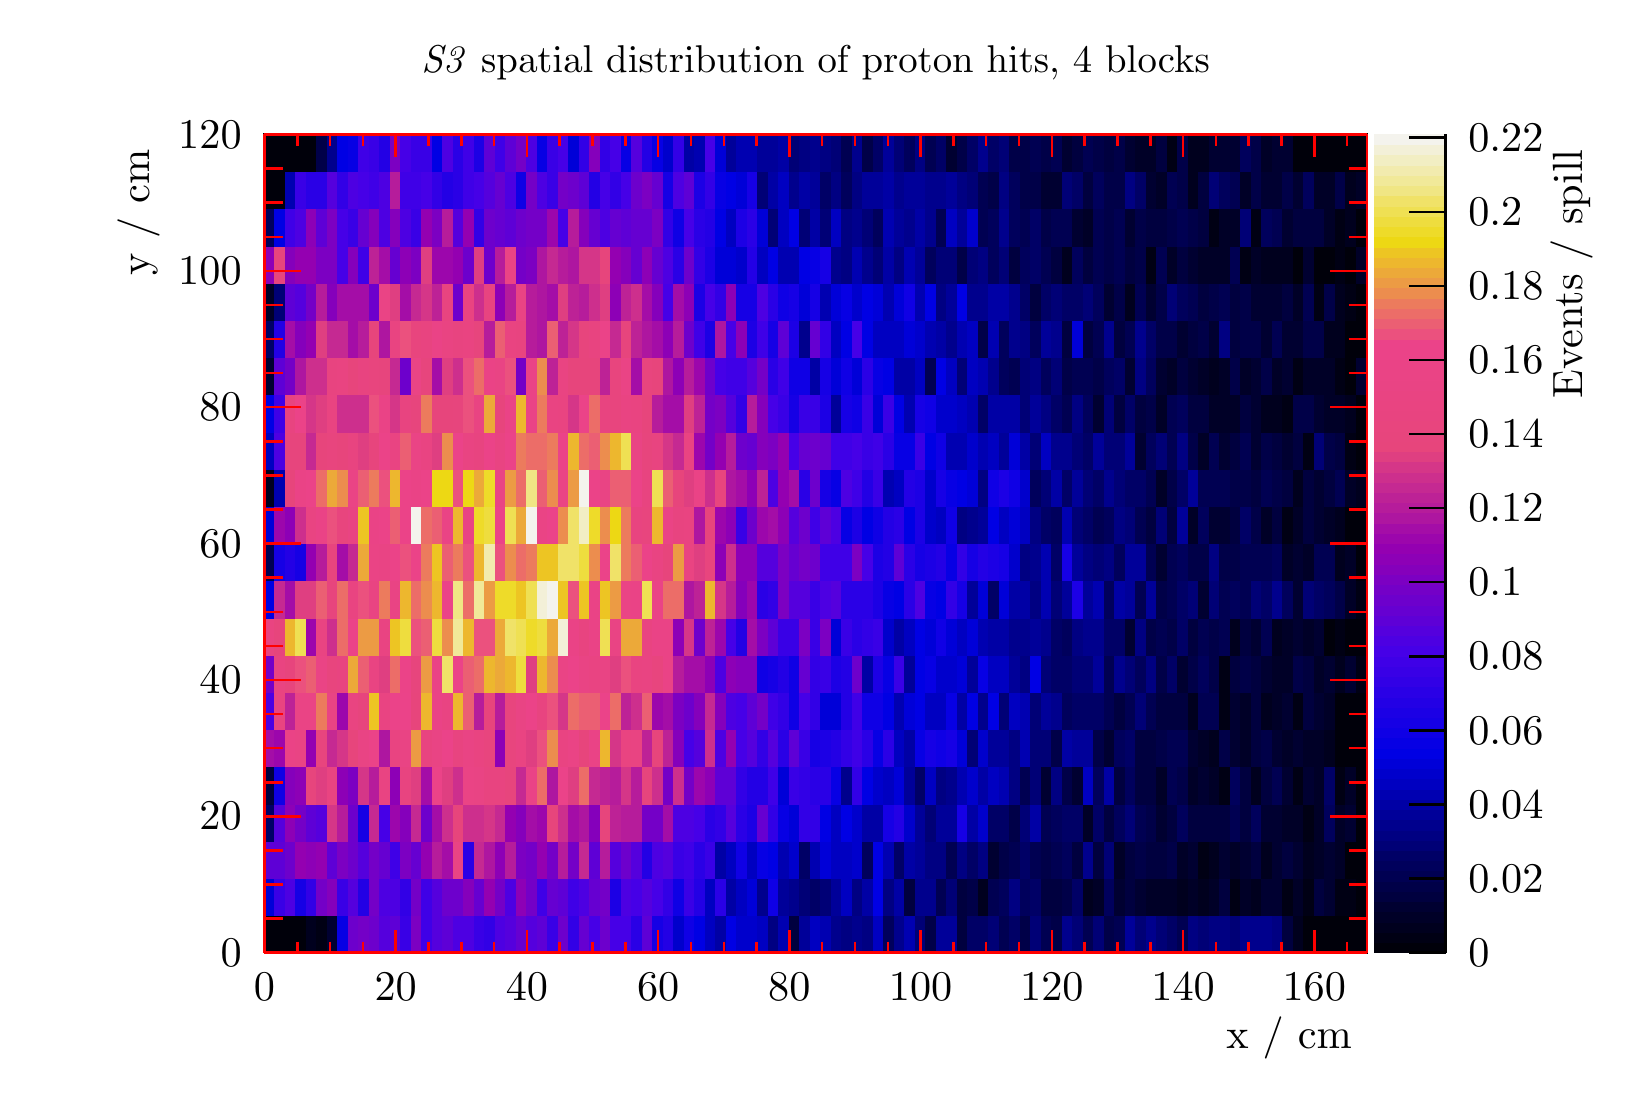
\begin{tikzpicture}
\pgfdeclareplotmark{cross} {
\pgfpathmoveto{\pgfpoint{-0.3\pgfplotmarksize}{\pgfplotmarksize}}
\pgfpathlineto{\pgfpoint{+0.3\pgfplotmarksize}{\pgfplotmarksize}}
\pgfpathlineto{\pgfpoint{+0.3\pgfplotmarksize}{0.3\pgfplotmarksize}}
\pgfpathlineto{\pgfpoint{+1\pgfplotmarksize}{0.3\pgfplotmarksize}}
\pgfpathlineto{\pgfpoint{+1\pgfplotmarksize}{-0.3\pgfplotmarksize}}
\pgfpathlineto{\pgfpoint{+0.3\pgfplotmarksize}{-0.3\pgfplotmarksize}}
\pgfpathlineto{\pgfpoint{+0.3\pgfplotmarksize}{-1.\pgfplotmarksize}}
\pgfpathlineto{\pgfpoint{-0.3\pgfplotmarksize}{-1.\pgfplotmarksize}}
\pgfpathlineto{\pgfpoint{-0.3\pgfplotmarksize}{-0.3\pgfplotmarksize}}
\pgfpathlineto{\pgfpoint{-1.\pgfplotmarksize}{-0.3\pgfplotmarksize}}
\pgfpathlineto{\pgfpoint{-1.\pgfplotmarksize}{0.3\pgfplotmarksize}}
\pgfpathlineto{\pgfpoint{-0.3\pgfplotmarksize}{0.3\pgfplotmarksize}}
\pgfpathclose
\pgfusepathqstroke
}
\pgfdeclareplotmark{cross*} {
\pgfpathmoveto{\pgfpoint{-0.3\pgfplotmarksize}{\pgfplotmarksize}}
\pgfpathlineto{\pgfpoint{+0.3\pgfplotmarksize}{\pgfplotmarksize}}
\pgfpathlineto{\pgfpoint{+0.3\pgfplotmarksize}{0.3\pgfplotmarksize}}
\pgfpathlineto{\pgfpoint{+1\pgfplotmarksize}{0.3\pgfplotmarksize}}
\pgfpathlineto{\pgfpoint{+1\pgfplotmarksize}{-0.3\pgfplotmarksize}}
\pgfpathlineto{\pgfpoint{+0.3\pgfplotmarksize}{-0.3\pgfplotmarksize}}
\pgfpathlineto{\pgfpoint{+0.3\pgfplotmarksize}{-1.\pgfplotmarksize}}
\pgfpathlineto{\pgfpoint{-0.3\pgfplotmarksize}{-1.\pgfplotmarksize}}
\pgfpathlineto{\pgfpoint{-0.3\pgfplotmarksize}{-0.3\pgfplotmarksize}}
\pgfpathlineto{\pgfpoint{-1.\pgfplotmarksize}{-0.3\pgfplotmarksize}}
\pgfpathlineto{\pgfpoint{-1.\pgfplotmarksize}{0.3\pgfplotmarksize}}
\pgfpathlineto{\pgfpoint{-0.3\pgfplotmarksize}{0.3\pgfplotmarksize}}
\pgfpathclose
\pgfusepathqfillstroke
}
\pgfdeclareplotmark{newstar} {
\pgfpathmoveto{\pgfqpoint{0pt}{\pgfplotmarksize}}
\pgfpathlineto{\pgfqpointpolar{44}{0.5\pgfplotmarksize}}
\pgfpathlineto{\pgfqpointpolar{18}{\pgfplotmarksize}}
\pgfpathlineto{\pgfqpointpolar{-20}{0.5\pgfplotmarksize}}
\pgfpathlineto{\pgfqpointpolar{-54}{\pgfplotmarksize}}
\pgfpathlineto{\pgfqpointpolar{-90}{0.5\pgfplotmarksize}}
\pgfpathlineto{\pgfqpointpolar{234}{\pgfplotmarksize}}
\pgfpathlineto{\pgfqpointpolar{198}{0.5\pgfplotmarksize}}
\pgfpathlineto{\pgfqpointpolar{162}{\pgfplotmarksize}}
\pgfpathlineto{\pgfqpointpolar{134}{0.5\pgfplotmarksize}}
\pgfpathclose
\pgfusepathqstroke
}
\pgfdeclareplotmark{newstar*} {
\pgfpathmoveto{\pgfqpoint{0pt}{\pgfplotmarksize}}
\pgfpathlineto{\pgfqpointpolar{44}{0.5\pgfplotmarksize}}
\pgfpathlineto{\pgfqpointpolar{18}{\pgfplotmarksize}}
\pgfpathlineto{\pgfqpointpolar{-20}{0.5\pgfplotmarksize}}
\pgfpathlineto{\pgfqpointpolar{-54}{\pgfplotmarksize}}
\pgfpathlineto{\pgfqpointpolar{-90}{0.5\pgfplotmarksize}}
\pgfpathlineto{\pgfqpointpolar{234}{\pgfplotmarksize}}
\pgfpathlineto{\pgfqpointpolar{198}{0.5\pgfplotmarksize}}
\pgfpathlineto{\pgfqpointpolar{162}{\pgfplotmarksize}}
\pgfpathlineto{\pgfqpointpolar{134}{0.5\pgfplotmarksize}}
\pgfpathclose
\pgfusepathqfillstroke
}
\definecolor{c}{rgb}{1,1,1};
\draw [color=c, fill=c] (0,0) rectangle (20,13.4957);
\draw [color=c, fill=c] (3,1.75444) rectangle (17,12.1461);
\definecolor{c}{rgb}{0,0,0};
\draw [c,line width=0.9] (3,1.75444) -- (3,12.1461) -- (17,12.1461) -- (17,1.75444) -- (3,1.75444);
\definecolor{c}{rgb}{1,1,1};
\draw [color=c, fill=c] (3,1.75444) rectangle (17,12.1461);
\definecolor{c}{rgb}{0,0,0};
\draw [c,line width=0.9] (3,1.75444) -- (3,12.1461) -- (17,12.1461) -- (17,1.75444) -- (3,1.75444);
\definecolor{c}{rgb}{0,0,0.0387097};
\draw [color=c, fill=c] (3,1.75444) rectangle (3.13333,2.22679);
\draw [color=c, fill=c] (3.13333,1.75444) rectangle (3.26667,2.22679);
\draw [color=c, fill=c] (3.26667,1.75444) rectangle (3.4,2.22679);
\draw [color=c, fill=c] (3.4,1.75444) rectangle (3.53333,2.22679);
\definecolor{c}{rgb}{0,0,0.116129};
\draw [color=c, fill=c] (3.53333,1.75444) rectangle (3.66667,2.22679);
\definecolor{c}{rgb}{0,0,0.0774194};
\draw [color=c, fill=c] (3.66667,1.75444) rectangle (3.8,2.22679);
\definecolor{c}{rgb}{0,0,0.193548};
\draw [color=c, fill=c] (3.8,1.75444) rectangle (3.93333,2.22679);
\definecolor{c}{rgb}{0.0257353,0,0.895221};
\draw [color=c, fill=c] (3.93333,1.75444) rectangle (4.06667,2.22679);
\definecolor{c}{rgb}{0.427451,0,0.8};
\draw [color=c, fill=c] (4.06667,1.75444) rectangle (4.2,2.22679);
\definecolor{c}{rgb}{0.456127,0,0.780147};
\draw [color=c, fill=c] (4.2,1.75444) rectangle (4.33333,2.22679);
\definecolor{c}{rgb}{0.427451,0,0.8};
\draw [color=c, fill=c] (4.33333,1.75444) rectangle (4.46667,2.22679);
\definecolor{c}{rgb}{0.331863,0,0.866176};
\draw [color=c, fill=c] (4.46667,1.75444) rectangle (4.6,2.22679);
\definecolor{c}{rgb}{0.370098,0,0.839706};
\draw [color=c, fill=c] (4.6,1.75444) rectangle (4.73333,2.22679);
\definecolor{c}{rgb}{0.223039,0,0.903676};
\draw [color=c, fill=c] (4.73333,1.75444) rectangle (4.86667,2.22679);
\definecolor{c}{rgb}{0.484804,0,0.760294};
\draw [color=c, fill=c] (4.86667,1.75444) rectangle (5,2.22679);
\definecolor{c}{rgb}{0.248775,0,0.904779};
\draw [color=c, fill=c] (5,1.75444) rectangle (5.13333,2.22679);
\definecolor{c}{rgb}{0.331863,0,0.866176};
\draw [color=c, fill=c] (5.13333,1.75444) rectangle (5.26667,2.22679);
\definecolor{c}{rgb}{0.370098,0,0.839706};
\draw [color=c, fill=c] (5.26667,1.75444) rectangle (5.4,2.22679);
\definecolor{c}{rgb}{0.303186,0,0.886029};
\draw [color=c, fill=c] (5.4,1.75444) rectangle (5.53333,2.22679);
\draw [color=c, fill=c] (5.53333,1.75444) rectangle (5.66667,2.22679);
\definecolor{c}{rgb}{0.223039,0,0.903676};
\draw [color=c, fill=c] (5.66667,1.75444) rectangle (5.8,2.22679);
\definecolor{c}{rgb}{0.197304,0,0.902574};
\draw [color=c, fill=c] (5.8,1.75444) rectangle (5.93333,2.22679);
\definecolor{c}{rgb}{0.303186,0,0.886029};
\draw [color=c, fill=c] (5.93333,1.75444) rectangle (6.06667,2.22679);
\definecolor{c}{rgb}{0.331863,0,0.866176};
\draw [color=c, fill=c] (6.06667,1.75444) rectangle (6.2,2.22679);
\definecolor{c}{rgb}{0.398775,0,0.819853};
\draw [color=c, fill=c] (6.2,1.75444) rectangle (6.33333,2.22679);
\definecolor{c}{rgb}{0.331863,0,0.866176};
\draw [color=c, fill=c] (6.33333,1.75444) rectangle (6.46667,2.22679);
\definecolor{c}{rgb}{0.370098,0,0.839706};
\draw [color=c, fill=c] (6.46667,1.75444) rectangle (6.6,2.22679);
\definecolor{c}{rgb}{0.223039,0,0.903676};
\draw [color=c, fill=c] (6.6,1.75444) rectangle (6.73333,2.22679);
\definecolor{c}{rgb}{0.427451,0,0.8};
\draw [color=c, fill=c] (6.73333,1.75444) rectangle (6.86667,2.22679);
\definecolor{c}{rgb}{0.197304,0,0.902574};
\draw [color=c, fill=c] (6.86667,1.75444) rectangle (7,2.22679);
\definecolor{c}{rgb}{0.398775,0,0.819853};
\draw [color=c, fill=c] (7,1.75444) rectangle (7.13333,2.22679);
\definecolor{c}{rgb}{0.27451,0,0.905882};
\draw [color=c, fill=c] (7.13333,1.75444) rectangle (7.26667,2.22679);
\definecolor{c}{rgb}{0.427451,0,0.8};
\draw [color=c, fill=c] (7.26667,1.75444) rectangle (7.4,2.22679);
\definecolor{c}{rgb}{0.27451,0,0.905882};
\draw [color=c, fill=c] (7.4,1.75444) rectangle (7.53333,2.22679);
\draw [color=c, fill=c] (7.53333,1.75444) rectangle (7.66667,2.22679);
\definecolor{c}{rgb}{0.16299,0,0.901103};
\draw [color=c, fill=c] (7.66667,1.75444) rectangle (7.8,2.22679);
\definecolor{c}{rgb}{0.370098,0,0.839706};
\draw [color=c, fill=c] (7.8,1.75444) rectangle (7.93333,2.22679);
\definecolor{c}{rgb}{0.0857843,0,0.897794};
\draw [color=c, fill=c] (7.93333,1.75444) rectangle (8.06667,2.22679);
\definecolor{c}{rgb}{0.137255,0,0.9};
\draw [color=c, fill=c] (8.06667,1.75444) rectangle (8.2,2.22679);
\definecolor{c}{rgb}{0,0,0.801471};
\draw [color=c, fill=c] (8.2,1.75444) rectangle (8.33333,2.22679);
\definecolor{c}{rgb}{0.060049,0,0.896691};
\draw [color=c, fill=c] (8.33333,1.75444) rectangle (8.46667,2.22679);
\definecolor{c}{rgb}{0,0,0.894118};
\draw [color=c, fill=c] (8.46667,1.75444) rectangle (8.6,2.22679);
\definecolor{c}{rgb}{0,0,0.755147};
\draw [color=c, fill=c] (8.6,1.75444) rectangle (8.73333,2.22679);
\definecolor{c}{rgb}{0,0,0.647059};
\draw [color=c, fill=c] (8.73333,1.75444) rectangle (8.86667,2.22679);
\definecolor{c}{rgb}{0,0,0.894118};
\draw [color=c, fill=c] (8.86667,1.75444) rectangle (9,2.22679);
\definecolor{c}{rgb}{0,0,0.801471};
\draw [color=c, fill=c] (9,1.75444) rectangle (9.13333,2.22679);
\draw [color=c, fill=c] (9.13333,1.75444) rectangle (9.26667,2.22679);
\definecolor{c}{rgb}{0,0,0.755147};
\draw [color=c, fill=c] (9.26667,1.75444) rectangle (9.4,2.22679);
\definecolor{c}{rgb}{0,0,0.508088};
\draw [color=c, fill=c] (9.4,1.75444) rectangle (9.53333,2.22679);
\definecolor{c}{rgb}{0,0,0.693382};
\draw [color=c, fill=c] (9.53333,1.75444) rectangle (9.66667,2.22679);
\definecolor{c}{rgb}{0,0,0.245161};
\draw [color=c, fill=c] (9.66667,1.75444) rectangle (9.8,2.22679);
\definecolor{c}{rgb}{0,0,0.600735};
\draw [color=c, fill=c] (9.8,1.75444) rectangle (9.93333,2.22679);
\definecolor{c}{rgb}{0,0,0.755147};
\draw [color=c, fill=c] (9.93333,1.75444) rectangle (10.0667,2.22679);
\definecolor{c}{rgb}{0,0,0.693382};
\draw [color=c, fill=c] (10.0667,1.75444) rectangle (10.2,2.22679);
\definecolor{c}{rgb}{0,0,0.554412};
\draw [color=c, fill=c] (10.2,1.75444) rectangle (10.3333,2.22679);
\definecolor{c}{rgb}{0,0,0.508088};
\draw [color=c, fill=c] (10.3333,1.75444) rectangle (10.4667,2.22679);
\definecolor{c}{rgb}{0,0,0.554412};
\draw [color=c, fill=c] (10.4667,1.75444) rectangle (10.6,2.22679);
\definecolor{c}{rgb}{0,0,0.508088};
\draw [color=c, fill=c] (10.6,1.75444) rectangle (10.7333,2.22679);
\definecolor{c}{rgb}{0,0,0.755147};
\draw [color=c, fill=c] (10.7333,1.75444) rectangle (10.8667,2.22679);
\definecolor{c}{rgb}{0,0,0.36129};
\draw [color=c, fill=c] (10.8667,1.75444) rectangle (11,2.22679);
\definecolor{c}{rgb}{0,0,0.554412};
\draw [color=c, fill=c] (11,1.75444) rectangle (11.1333,2.22679);
\definecolor{c}{rgb}{0,0,0.693382};
\draw [color=c, fill=c] (11.1333,1.75444) rectangle (11.2667,2.22679);
\definecolor{c}{rgb}{0,0,0.461765};
\draw [color=c, fill=c] (11.2667,1.75444) rectangle (11.4,2.22679);
\definecolor{c}{rgb}{0,0,0.283871};
\draw [color=c, fill=c] (11.4,1.75444) rectangle (11.5333,2.22679);
\definecolor{c}{rgb}{0,0,0.600735};
\draw [color=c, fill=c] (11.5333,1.75444) rectangle (11.6667,2.22679);
\draw [color=c, fill=c] (11.6667,1.75444) rectangle (11.8,2.22679);
\definecolor{c}{rgb}{0,0,0.245161};
\draw [color=c, fill=c] (11.8,1.75444) rectangle (11.9333,2.22679);
\definecolor{c}{rgb}{0,0,0.4};
\draw [color=c, fill=c] (11.9333,1.75444) rectangle (12.0667,2.22679);
\draw [color=c, fill=c] (12.0667,1.75444) rectangle (12.2,2.22679);
\definecolor{c}{rgb}{0,0,0.461765};
\draw [color=c, fill=c] (12.2,1.75444) rectangle (12.3333,2.22679);
\definecolor{c}{rgb}{0,0,0.322581};
\draw [color=c, fill=c] (12.3333,1.75444) rectangle (12.4667,2.22679);
\definecolor{c}{rgb}{0,0,0.4};
\draw [color=c, fill=c] (12.4667,1.75444) rectangle (12.6,2.22679);
\definecolor{c}{rgb}{0,0,0.283871};
\draw [color=c, fill=c] (12.6,1.75444) rectangle (12.7333,2.22679);
\definecolor{c}{rgb}{0,0,0.461765};
\draw [color=c, fill=c] (12.7333,1.75444) rectangle (12.8667,2.22679);
\definecolor{c}{rgb}{0,0,0.322581};
\draw [color=c, fill=c] (12.8667,1.75444) rectangle (13,2.22679);
\definecolor{c}{rgb}{0,0,0.283871};
\draw [color=c, fill=c] (13,1.75444) rectangle (13.1333,2.22679);
\definecolor{c}{rgb}{0,0,0.554412};
\draw [color=c, fill=c] (13.1333,1.75444) rectangle (13.2667,2.22679);
\definecolor{c}{rgb}{0,0,0.461765};
\draw [color=c, fill=c] (13.2667,1.75444) rectangle (13.4,2.22679);
\definecolor{c}{rgb}{0,0,0.322581};
\draw [color=c, fill=c] (13.4,1.75444) rectangle (13.5333,2.22679);
\definecolor{c}{rgb}{0,0,0.461765};
\draw [color=c, fill=c] (13.5333,1.75444) rectangle (13.6667,2.22679);
\definecolor{c}{rgb}{0,0,0.283871};
\draw [color=c, fill=c] (13.6667,1.75444) rectangle (13.8,2.22679);
\definecolor{c}{rgb}{0,0,0.322581};
\draw [color=c, fill=c] (13.8,1.75444) rectangle (13.9333,2.22679);
\definecolor{c}{rgb}{0,0,0.600735};
\draw [color=c, fill=c] (13.9333,1.75444) rectangle (14.0667,2.22679);
\definecolor{c}{rgb}{0,0,0.461765};
\draw [color=c, fill=c] (14.0667,1.75444) rectangle (14.2,2.22679);
\definecolor{c}{rgb}{0,0,0.554412};
\draw [color=c, fill=c] (14.2,1.75444) rectangle (14.3333,2.22679);
\definecolor{c}{rgb}{0,0,0.461765};
\draw [color=c, fill=c] (14.3333,1.75444) rectangle (14.4667,2.22679);
\definecolor{c}{rgb}{0,0,0.4};
\draw [color=c, fill=c] (14.4667,1.75444) rectangle (14.6,2.22679);
\definecolor{c}{rgb}{0,0,0.322581};
\draw [color=c, fill=c] (14.6,1.75444) rectangle (14.7333,2.22679);
\definecolor{c}{rgb}{0,0,0.508088};
\draw [color=c, fill=c] (14.7333,1.75444) rectangle (14.8667,2.22679);
\definecolor{c}{rgb}{0,0,0.461765};
\draw [color=c, fill=c] (14.8667,1.75444) rectangle (15,2.22679);
\definecolor{c}{rgb}{0,0,0.508088};
\draw [color=c, fill=c] (15,1.75444) rectangle (15.1333,2.22679);
\draw [color=c, fill=c] (15.1333,1.75444) rectangle (15.2667,2.22679);
\definecolor{c}{rgb}{0,0,0.461765};
\draw [color=c, fill=c] (15.2667,1.75444) rectangle (15.4,2.22679);
\definecolor{c}{rgb}{0,0,0.554412};
\draw [color=c, fill=c] (15.4,1.75444) rectangle (15.5333,2.22679);
\draw [color=c, fill=c] (15.5333,1.75444) rectangle (15.6667,2.22679);
\draw [color=c, fill=c] (15.6667,1.75444) rectangle (15.8,2.22679);
\definecolor{c}{rgb}{0,0,0.508088};
\draw [color=c, fill=c] (15.8,1.75444) rectangle (15.9333,2.22679);
\definecolor{c}{rgb}{0,0,0.245161};
\draw [color=c, fill=c] (15.9333,1.75444) rectangle (16.0667,2.22679);
\definecolor{c}{rgb}{0,0,0.116129};
\draw [color=c, fill=c] (16.0667,1.75444) rectangle (16.2,2.22679);
\definecolor{c}{rgb}{0,0,0.0387097};
\draw [color=c, fill=c] (16.2,1.75444) rectangle (16.3333,2.22679);
\draw [color=c, fill=c] (16.3333,1.75444) rectangle (16.4667,2.22679);
\draw [color=c, fill=c] (16.4667,1.75444) rectangle (16.6,2.22679);
\draw [color=c, fill=c] (16.6,1.75444) rectangle (16.7333,2.22679);
\draw [color=c, fill=c] (16.7333,1.75444) rectangle (16.8667,2.22679);
\draw [color=c, fill=c] (16.8667,1.75444) rectangle (17,2.22679);
\definecolor{c}{rgb}{0,0,0.847794};
\draw [color=c, fill=c] (3,2.22679) rectangle (3.13333,2.69914);
\definecolor{c}{rgb}{0.223039,0,0.903676};
\draw [color=c, fill=c] (3.13333,2.22679) rectangle (3.26667,2.69914);
\definecolor{c}{rgb}{0.303186,0,0.886029};
\draw [color=c, fill=c] (3.26667,2.22679) rectangle (3.4,2.69914);
\definecolor{c}{rgb}{0.0857843,0,0.897794};
\draw [color=c, fill=c] (3.4,2.22679) rectangle (3.53333,2.69914);
\definecolor{c}{rgb}{0.197304,0,0.902574};
\draw [color=c, fill=c] (3.53333,2.22679) rectangle (3.66667,2.69914);
\definecolor{c}{rgb}{0.456127,0,0.780147};
\draw [color=c, fill=c] (3.66667,2.22679) rectangle (3.8,2.69914);
\definecolor{c}{rgb}{0.523039,0,0.733824};
\draw [color=c, fill=c] (3.8,2.22679) rectangle (3.93333,2.69914);
\definecolor{c}{rgb}{0.223039,0,0.903676};
\draw [color=c, fill=c] (3.93333,2.22679) rectangle (4.06667,2.69914);
\definecolor{c}{rgb}{0.331863,0,0.866176};
\draw [color=c, fill=c] (4.06667,2.22679) rectangle (4.2,2.69914);
\definecolor{c}{rgb}{0.137255,0,0.9};
\draw [color=c, fill=c] (4.2,2.22679) rectangle (4.33333,2.69914);
\definecolor{c}{rgb}{0.456127,0,0.780147};
\draw [color=c, fill=c] (4.33333,2.22679) rectangle (4.46667,2.69914);
\definecolor{c}{rgb}{0.303186,0,0.886029};
\draw [color=c, fill=c] (4.46667,2.22679) rectangle (4.6,2.69914);
\draw [color=c, fill=c] (4.6,2.22679) rectangle (4.73333,2.69914);
\definecolor{c}{rgb}{0.197304,0,0.902574};
\draw [color=c, fill=c] (4.73333,2.22679) rectangle (4.86667,2.69914);
\definecolor{c}{rgb}{0.456127,0,0.780147};
\draw [color=c, fill=c] (4.86667,2.22679) rectangle (5,2.69914);
\definecolor{c}{rgb}{0.248775,0,0.904779};
\draw [color=c, fill=c] (5,2.22679) rectangle (5.13333,2.69914);
\definecolor{c}{rgb}{0.331863,0,0.866176};
\draw [color=c, fill=c] (5.13333,2.22679) rectangle (5.26667,2.69914);
\definecolor{c}{rgb}{0.427451,0,0.8};
\draw [color=c, fill=c] (5.26667,2.22679) rectangle (5.4,2.69914);
\draw [color=c, fill=c] (5.4,2.22679) rectangle (5.53333,2.69914);
\definecolor{c}{rgb}{0.523039,0,0.733824};
\draw [color=c, fill=c] (5.53333,2.22679) rectangle (5.66667,2.69914);
\definecolor{c}{rgb}{0.398775,0,0.819853};
\draw [color=c, fill=c] (5.66667,2.22679) rectangle (5.8,2.69914);
\definecolor{c}{rgb}{0.580392,0,0.694118};
\draw [color=c, fill=c] (5.8,2.22679) rectangle (5.93333,2.69914);
\definecolor{c}{rgb}{0.456127,0,0.780147};
\draw [color=c, fill=c] (5.93333,2.22679) rectangle (6.06667,2.69914);
\definecolor{c}{rgb}{0.303186,0,0.886029};
\draw [color=c, fill=c] (6.06667,2.22679) rectangle (6.2,2.69914);
\definecolor{c}{rgb}{0.551716,0,0.713971};
\draw [color=c, fill=c] (6.2,2.22679) rectangle (6.33333,2.69914);
\definecolor{c}{rgb}{0.456127,0,0.780147};
\draw [color=c, fill=c] (6.33333,2.22679) rectangle (6.46667,2.69914);
\definecolor{c}{rgb}{0.248775,0,0.904779};
\draw [color=c, fill=c] (6.46667,2.22679) rectangle (6.6,2.69914);
\definecolor{c}{rgb}{0.398775,0,0.819853};
\draw [color=c, fill=c] (6.6,2.22679) rectangle (6.73333,2.69914);
\definecolor{c}{rgb}{0.370098,0,0.839706};
\draw [color=c, fill=c] (6.73333,2.22679) rectangle (6.86667,2.69914);
\definecolor{c}{rgb}{0.248775,0,0.904779};
\draw [color=c, fill=c] (6.86667,2.22679) rectangle (7,2.69914);
\definecolor{c}{rgb}{0.303186,0,0.886029};
\draw [color=c, fill=c] (7,2.22679) rectangle (7.13333,2.69914);
\definecolor{c}{rgb}{0.398775,0,0.819853};
\draw [color=c, fill=c] (7.13333,2.22679) rectangle (7.26667,2.69914);
\definecolor{c}{rgb}{0.456127,0,0.780147};
\draw [color=c, fill=c] (7.26667,2.22679) rectangle (7.4,2.69914);
\definecolor{c}{rgb}{0.11152,0,0.898897};
\draw [color=c, fill=c] (7.4,2.22679) rectangle (7.53333,2.69914);
\definecolor{c}{rgb}{0.303186,0,0.886029};
\draw [color=c, fill=c] (7.53333,2.22679) rectangle (7.66667,2.69914);
\definecolor{c}{rgb}{0.27451,0,0.905882};
\draw [color=c, fill=c] (7.66667,2.22679) rectangle (7.8,2.69914);
\definecolor{c}{rgb}{0.331863,0,0.866176};
\draw [color=c, fill=c] (7.8,2.22679) rectangle (7.93333,2.69914);
\definecolor{c}{rgb}{0.27451,0,0.905882};
\draw [color=c, fill=c] (7.93333,2.22679) rectangle (8.06667,2.69914);
\definecolor{c}{rgb}{0.197304,0,0.902574};
\draw [color=c, fill=c] (8.06667,2.22679) rectangle (8.2,2.69914);
\definecolor{c}{rgb}{0.060049,0,0.896691};
\draw [color=c, fill=c] (8.2,2.22679) rectangle (8.33333,2.69914);
\definecolor{c}{rgb}{0.223039,0,0.903676};
\draw [color=c, fill=c] (8.33333,2.22679) rectangle (8.46667,2.69914);
\definecolor{c}{rgb}{0.137255,0,0.9};
\draw [color=c, fill=c] (8.46667,2.22679) rectangle (8.6,2.69914);
\definecolor{c}{rgb}{0,0,0.755147};
\draw [color=c, fill=c] (8.6,2.22679) rectangle (8.73333,2.69914);
\definecolor{c}{rgb}{0.16299,0,0.901103};
\draw [color=c, fill=c] (8.73333,2.22679) rectangle (8.86667,2.69914);
\definecolor{c}{rgb}{0,0,0.647059};
\draw [color=c, fill=c] (8.86667,2.22679) rectangle (9,2.69914);
\definecolor{c}{rgb}{0,0,0.755147};
\draw [color=c, fill=c] (9,2.22679) rectangle (9.13333,2.69914);
\definecolor{c}{rgb}{0,0,0.847794};
\draw [color=c, fill=c] (9.13333,2.22679) rectangle (9.26667,2.69914);
\definecolor{c}{rgb}{0,0,0.554412};
\draw [color=c, fill=c] (9.26667,2.22679) rectangle (9.4,2.69914);
\definecolor{c}{rgb}{0.060049,0,0.896691};
\draw [color=c, fill=c] (9.4,2.22679) rectangle (9.53333,2.69914);
\definecolor{c}{rgb}{0,0,0.600735};
\draw [color=c, fill=c] (9.53333,2.22679) rectangle (9.66667,2.69914);
\definecolor{c}{rgb}{0,0,0.554412};
\draw [color=c, fill=c] (9.66667,2.22679) rectangle (9.8,2.69914);
\definecolor{c}{rgb}{0,0,0.461765};
\draw [color=c, fill=c] (9.8,2.22679) rectangle (9.93333,2.69914);
\definecolor{c}{rgb}{0,0,0.4};
\draw [color=c, fill=c] (9.93333,2.22679) rectangle (10.0667,2.69914);
\definecolor{c}{rgb}{0,0,0.461765};
\draw [color=c, fill=c] (10.0667,2.22679) rectangle (10.2,2.69914);
\definecolor{c}{rgb}{0,0,0.600735};
\draw [color=c, fill=c] (10.2,2.22679) rectangle (10.3333,2.69914);
\definecolor{c}{rgb}{0,0,0.755147};
\draw [color=c, fill=c] (10.3333,2.22679) rectangle (10.4667,2.69914);
\definecolor{c}{rgb}{0,0,0.508088};
\draw [color=c, fill=c] (10.4667,2.22679) rectangle (10.6,2.69914);
\definecolor{c}{rgb}{0,0,0.647059};
\draw [color=c, fill=c] (10.6,2.22679) rectangle (10.7333,2.69914);
\definecolor{c}{rgb}{0,0,0.894118};
\draw [color=c, fill=c] (10.7333,2.22679) rectangle (10.8667,2.69914);
\definecolor{c}{rgb}{0,0,0.508088};
\draw [color=c, fill=c] (10.8667,2.22679) rectangle (11,2.69914);
\definecolor{c}{rgb}{0,0,0.647059};
\draw [color=c, fill=c] (11,2.22679) rectangle (11.1333,2.69914);
\definecolor{c}{rgb}{0,0,0.245161};
\draw [color=c, fill=c] (11.1333,2.22679) rectangle (11.2667,2.69914);
\definecolor{c}{rgb}{0,0,0.554412};
\draw [color=c, fill=c] (11.2667,2.22679) rectangle (11.4,2.69914);
\draw [color=c, fill=c] (11.4,2.22679) rectangle (11.5333,2.69914);
\definecolor{c}{rgb}{0,0,0.322581};
\draw [color=c, fill=c] (11.5333,2.22679) rectangle (11.6667,2.69914);
\definecolor{c}{rgb}{0,0,0.461765};
\draw [color=c, fill=c] (11.6667,2.22679) rectangle (11.8,2.69914);
\definecolor{c}{rgb}{0,0,0.245161};
\draw [color=c, fill=c] (11.8,2.22679) rectangle (11.9333,2.69914);
\definecolor{c}{rgb}{0,0,0.283871};
\draw [color=c, fill=c] (11.9333,2.22679) rectangle (12.0667,2.69914);
\definecolor{c}{rgb}{0,0,0.116129};
\draw [color=c, fill=c] (12.0667,2.22679) rectangle (12.2,2.69914);
\definecolor{c}{rgb}{0,0,0.322581};
\draw [color=c, fill=c] (12.2,2.22679) rectangle (12.3333,2.69914);
\definecolor{c}{rgb}{0,0,0.36129};
\draw [color=c, fill=c] (12.3333,2.22679) rectangle (12.4667,2.69914);
\definecolor{c}{rgb}{0,0,0.508088};
\draw [color=c, fill=c] (12.4667,2.22679) rectangle (12.6,2.69914);
\definecolor{c}{rgb}{0,0,0.36129};
\draw [color=c, fill=c] (12.6,2.22679) rectangle (12.7333,2.69914);
\definecolor{c}{rgb}{0,0,0.4};
\draw [color=c, fill=c] (12.7333,2.22679) rectangle (12.8667,2.69914);
\definecolor{c}{rgb}{0,0,0.245161};
\draw [color=c, fill=c] (12.8667,2.22679) rectangle (13,2.69914);
\draw [color=c, fill=c] (13,2.22679) rectangle (13.1333,2.69914);
\definecolor{c}{rgb}{0,0,0.283871};
\draw [color=c, fill=c] (13.1333,2.22679) rectangle (13.2667,2.69914);
\definecolor{c}{rgb}{0,0,0.4};
\draw [color=c, fill=c] (13.2667,2.22679) rectangle (13.4,2.69914);
\definecolor{c}{rgb}{0,0,0.116129};
\draw [color=c, fill=c] (13.4,2.22679) rectangle (13.5333,2.69914);
\definecolor{c}{rgb}{0,0,0.154839};
\draw [color=c, fill=c] (13.5333,2.22679) rectangle (13.6667,2.69914);
\definecolor{c}{rgb}{0,0,0.36129};
\draw [color=c, fill=c] (13.6667,2.22679) rectangle (13.8,2.69914);
\definecolor{c}{rgb}{0,0,0.193548};
\draw [color=c, fill=c] (13.8,2.22679) rectangle (13.9333,2.69914);
\definecolor{c}{rgb}{0,0,0.245161};
\draw [color=c, fill=c] (13.9333,2.22679) rectangle (14.0667,2.69914);
\definecolor{c}{rgb}{0,0,0.193548};
\draw [color=c, fill=c] (14.0667,2.22679) rectangle (14.2,2.69914);
\definecolor{c}{rgb}{0,0,0.154839};
\draw [color=c, fill=c] (14.2,2.22679) rectangle (14.3333,2.69914);
\draw [color=c, fill=c] (14.3333,2.22679) rectangle (14.4667,2.69914);
\draw [color=c, fill=c] (14.4667,2.22679) rectangle (14.6,2.69914);
\definecolor{c}{rgb}{0,0,0.116129};
\draw [color=c, fill=c] (14.6,2.22679) rectangle (14.7333,2.69914);
\definecolor{c}{rgb}{0,0,0.154839};
\draw [color=c, fill=c] (14.7333,2.22679) rectangle (14.8667,2.69914);
\definecolor{c}{rgb}{0,0,0.116129};
\draw [color=c, fill=c] (14.8667,2.22679) rectangle (15,2.69914);
\definecolor{c}{rgb}{0,0,0.154839};
\draw [color=c, fill=c] (15,2.22679) rectangle (15.1333,2.69914);
\definecolor{c}{rgb}{0,0,0.245161};
\draw [color=c, fill=c] (15.1333,2.22679) rectangle (15.2667,2.69914);
\definecolor{c}{rgb}{0,0,0.0774194};
\draw [color=c, fill=c] (15.2667,2.22679) rectangle (15.4,2.69914);
\definecolor{c}{rgb}{0,0,0.154839};
\draw [color=c, fill=c] (15.4,2.22679) rectangle (15.5333,2.69914);
\definecolor{c}{rgb}{0,0,0.116129};
\draw [color=c, fill=c] (15.5333,2.22679) rectangle (15.6667,2.69914);
\definecolor{c}{rgb}{0,0,0.193548};
\draw [color=c, fill=c] (15.6667,2.22679) rectangle (15.8,2.69914);
\draw [color=c, fill=c] (15.8,2.22679) rectangle (15.9333,2.69914);
\definecolor{c}{rgb}{0,0,0.0774194};
\draw [color=c, fill=c] (15.9333,2.22679) rectangle (16.0667,2.69914);
\definecolor{c}{rgb}{0,0,0.154839};
\draw [color=c, fill=c] (16.0667,2.22679) rectangle (16.2,2.69914);
\definecolor{c}{rgb}{0,0,0.0774194};
\draw [color=c, fill=c] (16.2,2.22679) rectangle (16.3333,2.69914);
\definecolor{c}{rgb}{0,0,0.245161};
\draw [color=c, fill=c] (16.3333,2.22679) rectangle (16.4667,2.69914);
\definecolor{c}{rgb}{0,0,0.193548};
\draw [color=c, fill=c] (16.4667,2.22679) rectangle (16.6,2.69914);
\definecolor{c}{rgb}{0,0,0.0774194};
\draw [color=c, fill=c] (16.6,2.22679) rectangle (16.7333,2.69914);
\draw [color=c, fill=c] (16.7333,2.22679) rectangle (16.8667,2.69914);
\definecolor{c}{rgb}{0,0,0.0387097};
\draw [color=c, fill=c] (16.8667,2.22679) rectangle (17,2.69914);
\definecolor{c}{rgb}{0.370098,0,0.839706};
\draw [color=c, fill=c] (3,2.69914) rectangle (3.13333,3.17149);
\draw [color=c, fill=c] (3.13333,2.69914) rectangle (3.26667,3.17149);
\definecolor{c}{rgb}{0.427451,0,0.8};
\draw [color=c, fill=c] (3.26667,2.69914) rectangle (3.4,3.17149);
\definecolor{c}{rgb}{0.580392,0,0.694118};
\draw [color=c, fill=c] (3.4,2.69914) rectangle (3.53333,3.17149);
\definecolor{c}{rgb}{0.551716,0,0.713971};
\draw [color=c, fill=c] (3.53333,2.69914) rectangle (3.66667,3.17149);
\definecolor{c}{rgb}{0.580392,0,0.694118};
\draw [color=c, fill=c] (3.66667,2.69914) rectangle (3.8,3.17149);
\definecolor{c}{rgb}{0.370098,0,0.839706};
\draw [color=c, fill=c] (3.8,2.69914) rectangle (3.93333,3.17149);
\definecolor{c}{rgb}{0.484804,0,0.760294};
\draw [color=c, fill=c] (3.93333,2.69914) rectangle (4.06667,3.17149);
\definecolor{c}{rgb}{0.427451,0,0.8};
\draw [color=c, fill=c] (4.06667,2.69914) rectangle (4.2,3.17149);
\definecolor{c}{rgb}{0.331863,0,0.866176};
\draw [color=c, fill=c] (4.2,2.69914) rectangle (4.33333,3.17149);
\definecolor{c}{rgb}{0.456127,0,0.780147};
\draw [color=c, fill=c] (4.33333,2.69914) rectangle (4.46667,3.17149);
\definecolor{c}{rgb}{0.398775,0,0.819853};
\draw [color=c, fill=c] (4.46667,2.69914) rectangle (4.6,3.17149);
\definecolor{c}{rgb}{0.248775,0,0.904779};
\draw [color=c, fill=c] (4.6,2.69914) rectangle (4.73333,3.17149);
\definecolor{c}{rgb}{0.484804,0,0.760294};
\draw [color=c, fill=c] (4.73333,2.69914) rectangle (4.86667,3.17149);
\definecolor{c}{rgb}{0.398775,0,0.819853};
\draw [color=c, fill=c] (4.86667,2.69914) rectangle (5,3.17149);
\definecolor{c}{rgb}{0.580392,0,0.694118};
\draw [color=c, fill=c] (5,2.69914) rectangle (5.13333,3.17149);
\definecolor{c}{rgb}{0.712623,0.109926,0.609681};
\draw [color=c, fill=c] (5.13333,2.69914) rectangle (5.26667,3.17149);
\definecolor{c}{rgb}{0.641422,0.0507353,0.655147};
\draw [color=c, fill=c] (5.26667,2.69914) rectangle (5.4,3.17149);
\definecolor{c}{rgb}{0.915196,0.265931,0.516544};
\draw [color=c, fill=c] (5.4,2.69914) rectangle (5.53333,3.17149);
\definecolor{c}{rgb}{0.16299,0,0.901103};
\draw [color=c, fill=c] (5.53333,2.69914) rectangle (5.66667,3.17149);
\definecolor{c}{rgb}{0.773652,0.160662,0.570711};
\draw [color=c, fill=c] (5.66667,2.69914) rectangle (5.8,3.17149);
\definecolor{c}{rgb}{0.682108,0.0845588,0.629167};
\draw [color=c, fill=c] (5.8,2.69914) rectangle (5.93333,3.17149);
\definecolor{c}{rgb}{0.551716,0,0.713971};
\draw [color=c, fill=c] (5.93333,2.69914) rectangle (6.06667,3.17149);
\definecolor{c}{rgb}{0.712623,0.109926,0.609681};
\draw [color=c, fill=c] (6.06667,2.69914) rectangle (6.2,3.17149);
\definecolor{c}{rgb}{0.484804,0,0.760294};
\draw [color=c, fill=c] (6.2,2.69914) rectangle (6.33333,3.17149);
\definecolor{c}{rgb}{0.456127,0,0.780147};
\draw [color=c, fill=c] (6.33333,2.69914) rectangle (6.46667,3.17149);
\definecolor{c}{rgb}{0.580392,0,0.694118};
\draw [color=c, fill=c] (6.46667,2.69914) rectangle (6.6,3.17149);
\definecolor{c}{rgb}{0.456127,0,0.780147};
\draw [color=c, fill=c] (6.6,2.69914) rectangle (6.73333,3.17149);
\definecolor{c}{rgb}{0.712623,0.109926,0.609681};
\draw [color=c, fill=c] (6.73333,2.69914) rectangle (6.86667,3.17149);
\definecolor{c}{rgb}{0.456127,0,0.780147};
\draw [color=c, fill=c] (6.86667,2.69914) rectangle (7,3.17149);
\definecolor{c}{rgb}{0.773652,0.160662,0.570711};
\draw [color=c, fill=c] (7,2.69914) rectangle (7.13333,3.17149);
\definecolor{c}{rgb}{0.370098,0,0.839706};
\draw [color=c, fill=c] (7.13333,2.69914) rectangle (7.26667,3.17149);
\definecolor{c}{rgb}{0.712623,0.109926,0.609681};
\draw [color=c, fill=c] (7.26667,2.69914) rectangle (7.4,3.17149);
\definecolor{c}{rgb}{0.331863,0,0.866176};
\draw [color=c, fill=c] (7.4,2.69914) rectangle (7.53333,3.17149);
\definecolor{c}{rgb}{0.427451,0,0.8};
\draw [color=c, fill=c] (7.53333,2.69914) rectangle (7.66667,3.17149);
\definecolor{c}{rgb}{0.331863,0,0.866176};
\draw [color=c, fill=c] (7.66667,2.69914) rectangle (7.8,3.17149);
\definecolor{c}{rgb}{0.137255,0,0.9};
\draw [color=c, fill=c] (7.8,2.69914) rectangle (7.93333,3.17149);
\definecolor{c}{rgb}{0.303186,0,0.886029};
\draw [color=c, fill=c] (7.93333,2.69914) rectangle (8.06667,3.17149);
\definecolor{c}{rgb}{0.331863,0,0.866176};
\draw [color=c, fill=c] (8.06667,2.69914) rectangle (8.2,3.17149);
\definecolor{c}{rgb}{0.223039,0,0.903676};
\draw [color=c, fill=c] (8.2,2.69914) rectangle (8.33333,3.17149);
\definecolor{c}{rgb}{0.248775,0,0.904779};
\draw [color=c, fill=c] (8.33333,2.69914) rectangle (8.46667,3.17149);
\definecolor{c}{rgb}{0.16299,0,0.901103};
\draw [color=c, fill=c] (8.46667,2.69914) rectangle (8.6,3.17149);
\definecolor{c}{rgb}{0.223039,0,0.903676};
\draw [color=c, fill=c] (8.6,2.69914) rectangle (8.73333,3.17149);
\definecolor{c}{rgb}{0,0,0.647059};
\draw [color=c, fill=c] (8.73333,2.69914) rectangle (8.86667,3.17149);
\definecolor{c}{rgb}{0,0,0.755147};
\draw [color=c, fill=c] (8.86667,2.69914) rectangle (9,3.17149);
\definecolor{c}{rgb}{0.060049,0,0.896691};
\draw [color=c, fill=c] (9,2.69914) rectangle (9.13333,3.17149);
\definecolor{c}{rgb}{0,0,0.755147};
\draw [color=c, fill=c] (9.13333,2.69914) rectangle (9.26667,3.17149);
\definecolor{c}{rgb}{0.0257353,0,0.895221};
\draw [color=c, fill=c] (9.26667,2.69914) rectangle (9.4,3.17149);
\definecolor{c}{rgb}{0,0,0.894118};
\draw [color=c, fill=c] (9.4,2.69914) rectangle (9.53333,3.17149);
\definecolor{c}{rgb}{0,0,0.693382};
\draw [color=c, fill=c] (9.53333,2.69914) rectangle (9.66667,3.17149);
\definecolor{c}{rgb}{0,0,0.801471};
\draw [color=c, fill=c] (9.66667,2.69914) rectangle (9.8,3.17149);
\definecolor{c}{rgb}{0,0,0.4};
\draw [color=c, fill=c] (9.8,2.69914) rectangle (9.93333,3.17149);
\definecolor{c}{rgb}{0,0,0.693382};
\draw [color=c, fill=c] (9.93333,2.69914) rectangle (10.0667,3.17149);
\definecolor{c}{rgb}{0,0,0.847794};
\draw [color=c, fill=c] (10.0667,2.69914) rectangle (10.2,3.17149);
\definecolor{c}{rgb}{0,0,0.755147};
\draw [color=c, fill=c] (10.2,2.69914) rectangle (10.3333,3.17149);
\draw [color=c, fill=c] (10.3333,2.69914) rectangle (10.4667,3.17149);
\definecolor{c}{rgb}{0,0,0.801471};
\draw [color=c, fill=c] (10.4667,2.69914) rectangle (10.6,3.17149);
\definecolor{c}{rgb}{0,0,0.36129};
\draw [color=c, fill=c] (10.6,2.69914) rectangle (10.7333,3.17149);
\definecolor{c}{rgb}{0,0,0.894118};
\draw [color=c, fill=c] (10.7333,2.69914) rectangle (10.8667,3.17149);
\definecolor{c}{rgb}{0,0,0.693382};
\draw [color=c, fill=c] (10.8667,2.69914) rectangle (11,3.17149);
\definecolor{c}{rgb}{0,0,0.4};
\draw [color=c, fill=c] (11,2.69914) rectangle (11.1333,3.17149);
\definecolor{c}{rgb}{0,0,0.647059};
\draw [color=c, fill=c] (11.1333,2.69914) rectangle (11.2667,3.17149);
\definecolor{c}{rgb}{0,0,0.600735};
\draw [color=c, fill=c] (11.2667,2.69914) rectangle (11.4,3.17149);
\definecolor{c}{rgb}{0,0,0.508088};
\draw [color=c, fill=c] (11.4,2.69914) rectangle (11.5333,3.17149);
\draw [color=c, fill=c] (11.5333,2.69914) rectangle (11.6667,3.17149);
\definecolor{c}{rgb}{0,0,0.322581};
\draw [color=c, fill=c] (11.6667,2.69914) rectangle (11.8,3.17149);
\definecolor{c}{rgb}{0,0,0.508088};
\draw [color=c, fill=c] (11.8,2.69914) rectangle (11.9333,3.17149);
\definecolor{c}{rgb}{0,0,0.4};
\draw [color=c, fill=c] (11.9333,2.69914) rectangle (12.0667,3.17149);
\definecolor{c}{rgb}{0,0,0.508088};
\draw [color=c, fill=c] (12.0667,2.69914) rectangle (12.2,3.17149);
\definecolor{c}{rgb}{0,0,0.193548};
\draw [color=c, fill=c] (12.2,2.69914) rectangle (12.3333,3.17149);
\definecolor{c}{rgb}{0,0,0.283871};
\draw [color=c, fill=c] (12.3333,2.69914) rectangle (12.4667,3.17149);
\definecolor{c}{rgb}{0,0,0.322581};
\draw [color=c, fill=c] (12.4667,2.69914) rectangle (12.6,3.17149);
\definecolor{c}{rgb}{0,0,0.4};
\draw [color=c, fill=c] (12.6,2.69914) rectangle (12.7333,3.17149);
\definecolor{c}{rgb}{0,0,0.322581};
\draw [color=c, fill=c] (12.7333,2.69914) rectangle (12.8667,3.17149);
\definecolor{c}{rgb}{0,0,0.283871};
\draw [color=c, fill=c] (12.8667,2.69914) rectangle (13,3.17149);
\definecolor{c}{rgb}{0,0,0.322581};
\draw [color=c, fill=c] (13,2.69914) rectangle (13.1333,3.17149);
\definecolor{c}{rgb}{0,0,0.36129};
\draw [color=c, fill=c] (13.1333,2.69914) rectangle (13.2667,3.17149);
\definecolor{c}{rgb}{0,0,0.245161};
\draw [color=c, fill=c] (13.2667,2.69914) rectangle (13.4,3.17149);
\definecolor{c}{rgb}{0,0,0.554412};
\draw [color=c, fill=c] (13.4,2.69914) rectangle (13.5333,3.17149);
\definecolor{c}{rgb}{0,0,0.245161};
\draw [color=c, fill=c] (13.5333,2.69914) rectangle (13.6667,3.17149);
\definecolor{c}{rgb}{0,0,0.461765};
\draw [color=c, fill=c] (13.6667,2.69914) rectangle (13.8,3.17149);
\definecolor{c}{rgb}{0,0,0.154839};
\draw [color=c, fill=c] (13.8,2.69914) rectangle (13.9333,3.17149);
\definecolor{c}{rgb}{0,0,0.245161};
\draw [color=c, fill=c] (13.9333,2.69914) rectangle (14.0667,3.17149);
\definecolor{c}{rgb}{0,0,0.283871};
\draw [color=c, fill=c] (14.0667,2.69914) rectangle (14.2,3.17149);
\definecolor{c}{rgb}{0,0,0.245161};
\draw [color=c, fill=c] (14.2,2.69914) rectangle (14.3333,3.17149);
\draw [color=c, fill=c] (14.3333,2.69914) rectangle (14.4667,3.17149);
\definecolor{c}{rgb}{0,0,0.283871};
\draw [color=c, fill=c] (14.4667,2.69914) rectangle (14.6,3.17149);
\definecolor{c}{rgb}{0,0,0.154839};
\draw [color=c, fill=c] (14.6,2.69914) rectangle (14.7333,3.17149);
\definecolor{c}{rgb}{0,0,0.193548};
\draw [color=c, fill=c] (14.7333,2.69914) rectangle (14.8667,3.17149);
\definecolor{c}{rgb}{0,0,0.0774194};
\draw [color=c, fill=c] (14.8667,2.69914) rectangle (15,3.17149);
\definecolor{c}{rgb}{0,0,0.116129};
\draw [color=c, fill=c] (15,2.69914) rectangle (15.1333,3.17149);
\definecolor{c}{rgb}{0,0,0.193548};
\draw [color=c, fill=c] (15.1333,2.69914) rectangle (15.2667,3.17149);
\definecolor{c}{rgb}{0,0,0.154839};
\draw [color=c, fill=c] (15.2667,2.69914) rectangle (15.4,3.17149);
\definecolor{c}{rgb}{0,0,0.193548};
\draw [color=c, fill=c] (15.4,2.69914) rectangle (15.5333,3.17149);
\definecolor{c}{rgb}{0,0,0.245161};
\draw [color=c, fill=c] (15.5333,2.69914) rectangle (15.6667,3.17149);
\definecolor{c}{rgb}{0,0,0.116129};
\draw [color=c, fill=c] (15.6667,2.69914) rectangle (15.8,3.17149);
\definecolor{c}{rgb}{0,0,0.193548};
\draw [color=c, fill=c] (15.8,2.69914) rectangle (15.9333,3.17149);
\definecolor{c}{rgb}{0,0,0.245161};
\draw [color=c, fill=c] (15.9333,2.69914) rectangle (16.0667,3.17149);
\definecolor{c}{rgb}{0,0,0.193548};
\draw [color=c, fill=c] (16.0667,2.69914) rectangle (16.2,3.17149);
\definecolor{c}{rgb}{0,0,0.116129};
\draw [color=c, fill=c] (16.2,2.69914) rectangle (16.3333,3.17149);
\definecolor{c}{rgb}{0,0,0.154839};
\draw [color=c, fill=c] (16.3333,2.69914) rectangle (16.4667,3.17149);
\definecolor{c}{rgb}{0,0,0.193548};
\draw [color=c, fill=c] (16.4667,2.69914) rectangle (16.6,3.17149);
\definecolor{c}{rgb}{0,0,0.154839};
\draw [color=c, fill=c] (16.6,2.69914) rectangle (16.7333,3.17149);
\definecolor{c}{rgb}{0,0,0.0387097};
\draw [color=c, fill=c] (16.7333,2.69914) rectangle (16.8667,3.17149);
\draw [color=c, fill=c] (16.8667,2.69914) rectangle (17,3.17149);
\definecolor{c}{rgb}{0,0,0.4};
\draw [color=c, fill=c] (3,3.17149) rectangle (3.13333,3.64384);
\definecolor{c}{rgb}{0.331863,0,0.866176};
\draw [color=c, fill=c] (3.13333,3.17149) rectangle (3.26667,3.64384);
\definecolor{c}{rgb}{0.551716,0,0.713971};
\draw [color=c, fill=c] (3.26667,3.17149) rectangle (3.4,3.64384);
\definecolor{c}{rgb}{0.456127,0,0.780147};
\draw [color=c, fill=c] (3.4,3.17149) rectangle (3.53333,3.64384);
\definecolor{c}{rgb}{0.370098,0,0.839706};
\draw [color=c, fill=c] (3.53333,3.17149) rectangle (3.66667,3.64384);
\definecolor{c}{rgb}{0.331863,0,0.866176};
\draw [color=c, fill=c] (3.66667,3.17149) rectangle (3.8,3.64384);
\definecolor{c}{rgb}{0.834681,0.211397,0.53174};
\draw [color=c, fill=c] (3.8,3.17149) rectangle (3.93333,3.64384);
\definecolor{c}{rgb}{0.712623,0.109926,0.609681};
\draw [color=c, fill=c] (3.93333,3.17149) rectangle (4.06667,3.64384);
\definecolor{c}{rgb}{0.427451,0,0.8};
\draw [color=c, fill=c] (4.06667,3.17149) rectangle (4.2,3.64384);
\definecolor{c}{rgb}{0.0857843,0,0.897794};
\draw [color=c, fill=c] (4.2,3.17149) rectangle (4.33333,3.64384);
\definecolor{c}{rgb}{0.773652,0.160662,0.570711};
\draw [color=c, fill=c] (4.33333,3.17149) rectangle (4.46667,3.64384);
\definecolor{c}{rgb}{0.27451,0,0.905882};
\draw [color=c, fill=c] (4.46667,3.17149) rectangle (4.6,3.64384);
\definecolor{c}{rgb}{0.610907,0.0253676,0.674632};
\draw [color=c, fill=c] (4.6,3.17149) rectangle (4.73333,3.64384);
\definecolor{c}{rgb}{0.523039,0,0.733824};
\draw [color=c, fill=c] (4.73333,3.17149) rectangle (4.86667,3.64384);
\definecolor{c}{rgb}{0.773652,0.160662,0.570711};
\draw [color=c, fill=c] (4.86667,3.17149) rectangle (5,3.64384);
\definecolor{c}{rgb}{0.427451,0,0.8};
\draw [color=c, fill=c] (5,3.17149) rectangle (5.13333,3.64384);
\definecolor{c}{rgb}{0.641422,0.0507353,0.655147};
\draw [color=c, fill=c] (5.13333,3.17149) rectangle (5.26667,3.64384);
\definecolor{c}{rgb}{0.804167,0.186029,0.551225};
\draw [color=c, fill=c] (5.26667,3.17149) rectangle (5.4,3.64384);
\definecolor{c}{rgb}{0.905882,0.270588,0.486275};
\draw [color=c, fill=c] (5.4,3.17149) rectangle (5.53333,3.64384);
\definecolor{c}{rgb}{0.804167,0.186029,0.551225};
\draw [color=c, fill=c] (5.53333,3.17149) rectangle (5.66667,3.64384);
\draw [color=c, fill=c] (5.66667,3.17149) rectangle (5.8,3.64384);
\definecolor{c}{rgb}{0.834681,0.211397,0.53174};
\draw [color=c, fill=c] (5.8,3.17149) rectangle (5.93333,3.64384);
\definecolor{c}{rgb}{0.773652,0.160662,0.570711};
\draw [color=c, fill=c] (5.93333,3.17149) rectangle (6.06667,3.64384);
\definecolor{c}{rgb}{0.580392,0,0.694118};
\draw [color=c, fill=c] (6.06667,3.17149) rectangle (6.2,3.64384);
\definecolor{c}{rgb}{0.523039,0,0.733824};
\draw [color=c, fill=c] (6.2,3.17149) rectangle (6.33333,3.64384);
\definecolor{c}{rgb}{0.641422,0.0507353,0.655147};
\draw [color=c, fill=c] (6.33333,3.17149) rectangle (6.46667,3.64384);
\definecolor{c}{rgb}{0.610907,0.0253676,0.674632};
\draw [color=c, fill=c] (6.46667,3.17149) rectangle (6.6,3.64384);
\definecolor{c}{rgb}{0.905882,0.270588,0.486275};
\draw [color=c, fill=c] (6.6,3.17149) rectangle (6.73333,3.64384);
\definecolor{c}{rgb}{0.804167,0.186029,0.551225};
\draw [color=c, fill=c] (6.73333,3.17149) rectangle (6.86667,3.64384);
\definecolor{c}{rgb}{0.641422,0.0507353,0.655147};
\draw [color=c, fill=c] (6.86667,3.17149) rectangle (7,3.64384);
\definecolor{c}{rgb}{0.682108,0.0845588,0.629167};
\draw [color=c, fill=c] (7,3.17149) rectangle (7.13333,3.64384);
\definecolor{c}{rgb}{0.523039,0,0.733824};
\draw [color=c, fill=c] (7.13333,3.17149) rectangle (7.26667,3.64384);
\definecolor{c}{rgb}{0.905882,0.270588,0.486275};
\draw [color=c, fill=c] (7.26667,3.17149) rectangle (7.4,3.64384);
\definecolor{c}{rgb}{0.743137,0.135294,0.590196};
\draw [color=c, fill=c] (7.4,3.17149) rectangle (7.53333,3.64384);
\definecolor{c}{rgb}{0.712623,0.109926,0.609681};
\draw [color=c, fill=c] (7.53333,3.17149) rectangle (7.66667,3.64384);
\draw [color=c, fill=c] (7.66667,3.17149) rectangle (7.8,3.64384);
\definecolor{c}{rgb}{0.456127,0,0.780147};
\draw [color=c, fill=c] (7.8,3.17149) rectangle (7.93333,3.64384);
\draw [color=c, fill=c] (7.93333,3.17149) rectangle (8.06667,3.64384);
\definecolor{c}{rgb}{0.641422,0.0507353,0.655147};
\draw [color=c, fill=c] (8.06667,3.17149) rectangle (8.2,3.64384);
\definecolor{c}{rgb}{0.303186,0,0.886029};
\draw [color=c, fill=c] (8.2,3.17149) rectangle (8.33333,3.64384);
\draw [color=c, fill=c] (8.33333,3.17149) rectangle (8.46667,3.64384);
\definecolor{c}{rgb}{0.27451,0,0.905882};
\draw [color=c, fill=c] (8.46667,3.17149) rectangle (8.6,3.64384);
\definecolor{c}{rgb}{0.16299,0,0.901103};
\draw [color=c, fill=c] (8.6,3.17149) rectangle (8.73333,3.64384);
\definecolor{c}{rgb}{0.197304,0,0.902574};
\draw [color=c, fill=c] (8.73333,3.17149) rectangle (8.86667,3.64384);
\definecolor{c}{rgb}{0.331863,0,0.866176};
\draw [color=c, fill=c] (8.86667,3.17149) rectangle (9,3.64384);
\definecolor{c}{rgb}{0.16299,0,0.901103};
\draw [color=c, fill=c] (9,3.17149) rectangle (9.13333,3.64384);
\definecolor{c}{rgb}{0.11152,0,0.898897};
\draw [color=c, fill=c] (9.13333,3.17149) rectangle (9.26667,3.64384);
\definecolor{c}{rgb}{0.398775,0,0.819853};
\draw [color=c, fill=c] (9.26667,3.17149) rectangle (9.4,3.64384);
\definecolor{c}{rgb}{0.197304,0,0.902574};
\draw [color=c, fill=c] (9.4,3.17149) rectangle (9.53333,3.64384);
\definecolor{c}{rgb}{0.0257353,0,0.895221};
\draw [color=c, fill=c] (9.53333,3.17149) rectangle (9.66667,3.64384);
\definecolor{c}{rgb}{0,0,0.847794};
\draw [color=c, fill=c] (9.66667,3.17149) rectangle (9.8,3.64384);
\definecolor{c}{rgb}{0.197304,0,0.902574};
\draw [color=c, fill=c] (9.8,3.17149) rectangle (9.93333,3.64384);
\draw [color=c, fill=c] (9.93333,3.17149) rectangle (10.0667,3.64384);
\definecolor{c}{rgb}{0,0,0.894118};
\draw [color=c, fill=c] (10.0667,3.17149) rectangle (10.2,3.64384);
\definecolor{c}{rgb}{0,0,0.755147};
\draw [color=c, fill=c] (10.2,3.17149) rectangle (10.3333,3.64384);
\definecolor{c}{rgb}{0,0,0.894118};
\draw [color=c, fill=c] (10.3333,3.17149) rectangle (10.4667,3.64384);
\definecolor{c}{rgb}{0,0,0.801471};
\draw [color=c, fill=c] (10.4667,3.17149) rectangle (10.6,3.64384);
\definecolor{c}{rgb}{0,0,0.647059};
\draw [color=c, fill=c] (10.6,3.17149) rectangle (10.7333,3.64384);
\draw [color=c, fill=c] (10.7333,3.17149) rectangle (10.8667,3.64384);
\definecolor{c}{rgb}{0.0857843,0,0.897794};
\draw [color=c, fill=c] (10.8667,3.17149) rectangle (11,3.64384);
\definecolor{c}{rgb}{0.137255,0,0.9};
\draw [color=c, fill=c] (11,3.17149) rectangle (11.1333,3.64384);
\definecolor{c}{rgb}{0,0,0.801471};
\draw [color=c, fill=c] (11.1333,3.17149) rectangle (11.2667,3.64384);
\definecolor{c}{rgb}{0,0,0.600735};
\draw [color=c, fill=c] (11.2667,3.17149) rectangle (11.4,3.64384);
\definecolor{c}{rgb}{0,0,0.461765};
\draw [color=c, fill=c] (11.4,3.17149) rectangle (11.5333,3.64384);
\definecolor{c}{rgb}{0,0,0.600735};
\draw [color=c, fill=c] (11.5333,3.17149) rectangle (11.6667,3.64384);
\draw [color=c, fill=c] (11.6667,3.17149) rectangle (11.8,3.64384);
\definecolor{c}{rgb}{0.0857843,0,0.897794};
\draw [color=c, fill=c] (11.8,3.17149) rectangle (11.9333,3.64384);
\definecolor{c}{rgb}{0,0,0.647059};
\draw [color=c, fill=c] (11.9333,3.17149) rectangle (12.0667,3.64384);
\definecolor{c}{rgb}{0,0,0.801471};
\draw [color=c, fill=c] (12.0667,3.17149) rectangle (12.2,3.64384);
\definecolor{c}{rgb}{0,0,0.4};
\draw [color=c, fill=c] (12.2,3.17149) rectangle (12.3333,3.64384);
\draw [color=c, fill=c] (12.3333,3.17149) rectangle (12.4667,3.64384);
\definecolor{c}{rgb}{0,0,0.283871};
\draw [color=c, fill=c] (12.4667,3.17149) rectangle (12.6,3.64384);
\definecolor{c}{rgb}{0,0,0.461765};
\draw [color=c, fill=c] (12.6,3.17149) rectangle (12.7333,3.64384);
\definecolor{c}{rgb}{0,0,0.647059};
\draw [color=c, fill=c] (12.7333,3.17149) rectangle (12.8667,3.64384);
\definecolor{c}{rgb}{0,0,0.322581};
\draw [color=c, fill=c] (12.8667,3.17149) rectangle (13,3.64384);
\definecolor{c}{rgb}{0,0,0.36129};
\draw [color=c, fill=c] (13,3.17149) rectangle (13.1333,3.64384);
\definecolor{c}{rgb}{0,0,0.4};
\draw [color=c, fill=c] (13.1333,3.17149) rectangle (13.2667,3.64384);
\draw [color=c, fill=c] (13.2667,3.17149) rectangle (13.4,3.64384);
\definecolor{c}{rgb}{0,0,0.154839};
\draw [color=c, fill=c] (13.4,3.17149) rectangle (13.5333,3.64384);
\definecolor{c}{rgb}{0,0,0.4};
\draw [color=c, fill=c] (13.5333,3.17149) rectangle (13.6667,3.64384);
\definecolor{c}{rgb}{0,0,0.245161};
\draw [color=c, fill=c] (13.6667,3.17149) rectangle (13.8,3.64384);
\definecolor{c}{rgb}{0,0,0.36129};
\draw [color=c, fill=c] (13.8,3.17149) rectangle (13.9333,3.64384);
\definecolor{c}{rgb}{0,0,0.461765};
\draw [color=c, fill=c] (13.9333,3.17149) rectangle (14.0667,3.64384);
\definecolor{c}{rgb}{0,0,0.322581};
\draw [color=c, fill=c] (14.0667,3.17149) rectangle (14.2,3.64384);
\definecolor{c}{rgb}{0,0,0.283871};
\draw [color=c, fill=c] (14.2,3.17149) rectangle (14.3333,3.64384);
\definecolor{c}{rgb}{0,0,0.193548};
\draw [color=c, fill=c] (14.3333,3.17149) rectangle (14.4667,3.64384);
\definecolor{c}{rgb}{0,0,0.245161};
\draw [color=c, fill=c] (14.4667,3.17149) rectangle (14.6,3.64384);
\definecolor{c}{rgb}{0,0,0.36129};
\draw [color=c, fill=c] (14.6,3.17149) rectangle (14.7333,3.64384);
\definecolor{c}{rgb}{0,0,0.245161};
\draw [color=c, fill=c] (14.7333,3.17149) rectangle (14.8667,3.64384);
\draw [color=c, fill=c] (14.8667,3.17149) rectangle (15,3.64384);
\draw [color=c, fill=c] (15,3.17149) rectangle (15.1333,3.64384);
\draw [color=c, fill=c] (15.1333,3.17149) rectangle (15.2667,3.64384);
\definecolor{c}{rgb}{0,0,0.322581};
\draw [color=c, fill=c] (15.2667,3.17149) rectangle (15.4,3.64384);
\definecolor{c}{rgb}{0,0,0.245161};
\draw [color=c, fill=c] (15.4,3.17149) rectangle (15.5333,3.64384);
\definecolor{c}{rgb}{0,0,0.36129};
\draw [color=c, fill=c] (15.5333,3.17149) rectangle (15.6667,3.64384);
\definecolor{c}{rgb}{0,0,0.193548};
\draw [color=c, fill=c] (15.6667,3.17149) rectangle (15.8,3.64384);
\draw [color=c, fill=c] (15.8,3.17149) rectangle (15.9333,3.64384);
\definecolor{c}{rgb}{0,0,0.154839};
\draw [color=c, fill=c] (15.9333,3.17149) rectangle (16.0667,3.64384);
\draw [color=c, fill=c] (16.0667,3.17149) rectangle (16.2,3.64384);
\definecolor{c}{rgb}{0,0,0.0774194};
\draw [color=c, fill=c] (16.2,3.17149) rectangle (16.3333,3.64384);
\definecolor{c}{rgb}{0,0,0.154839};
\draw [color=c, fill=c] (16.3333,3.17149) rectangle (16.4667,3.64384);
\definecolor{c}{rgb}{0,0,0.36129};
\draw [color=c, fill=c] (16.4667,3.17149) rectangle (16.6,3.64384);
\definecolor{c}{rgb}{0,0,0.154839};
\draw [color=c, fill=c] (16.6,3.17149) rectangle (16.7333,3.64384);
\definecolor{c}{rgb}{0,0,0.193548};
\draw [color=c, fill=c] (16.7333,3.17149) rectangle (16.8667,3.64384);
\definecolor{c}{rgb}{0,0,0.0387097};
\draw [color=c, fill=c] (16.8667,3.17149) rectangle (17,3.64384);
\definecolor{c}{rgb}{0,0,0.245161};
\draw [color=c, fill=c] (3,3.64384) rectangle (3.13333,4.11619);
\definecolor{c}{rgb}{0.060049,0,0.896691};
\draw [color=c, fill=c] (3.13333,3.64384) rectangle (3.26667,4.11619);
\definecolor{c}{rgb}{0.523039,0,0.733824};
\draw [color=c, fill=c] (3.26667,3.64384) rectangle (3.4,4.11619);
\definecolor{c}{rgb}{0.551716,0,0.713971};
\draw [color=c, fill=c] (3.4,3.64384) rectangle (3.53333,4.11619);
\definecolor{c}{rgb}{0.907353,0.269853,0.491054};
\draw [color=c, fill=c] (3.53333,3.64384) rectangle (3.66667,4.11619);
\definecolor{c}{rgb}{0.875368,0.245221,0.50576};
\draw [color=c, fill=c] (3.66667,3.64384) rectangle (3.8,4.11619);
\definecolor{c}{rgb}{0.912255,0.267402,0.506985};
\draw [color=c, fill=c] (3.8,3.64384) rectangle (3.93333,4.11619);
\definecolor{c}{rgb}{0.551716,0,0.713971};
\draw [color=c, fill=c] (3.93333,3.64384) rectangle (4.06667,4.11619);
\definecolor{c}{rgb}{0.484804,0,0.760294};
\draw [color=c, fill=c] (4.06667,3.64384) rectangle (4.2,4.11619);
\definecolor{c}{rgb}{0.834681,0.211397,0.53174};
\draw [color=c, fill=c] (4.2,3.64384) rectangle (4.33333,4.11619);
\definecolor{c}{rgb}{0.712623,0.109926,0.609681};
\draw [color=c, fill=c] (4.33333,3.64384) rectangle (4.46667,4.11619);
\definecolor{c}{rgb}{0.913725,0.266667,0.511765};
\draw [color=c, fill=c] (4.46667,3.64384) rectangle (4.6,4.11619);
\definecolor{c}{rgb}{0.551716,0,0.713971};
\draw [color=c, fill=c] (4.6,3.64384) rectangle (4.73333,4.11619);
\definecolor{c}{rgb}{0.910294,0.268382,0.500613};
\draw [color=c, fill=c] (4.73333,3.64384) rectangle (4.86667,4.11619);
\definecolor{c}{rgb}{0.875368,0.245221,0.50576};
\draw [color=c, fill=c] (4.86667,3.64384) rectangle (5,4.11619);
\definecolor{c}{rgb}{0.641422,0.0507353,0.655147};
\draw [color=c, fill=c] (5,3.64384) rectangle (5.13333,4.11619);
\definecolor{c}{rgb}{0.920098,0.26348,0.532475};
\draw [color=c, fill=c] (5.13333,3.64384) rectangle (5.26667,4.11619);
\definecolor{c}{rgb}{0.875368,0.245221,0.50576};
\draw [color=c, fill=c] (5.26667,3.64384) rectangle (5.4,4.11619);
\definecolor{c}{rgb}{0.804167,0.186029,0.551225};
\draw [color=c, fill=c] (5.4,3.64384) rectangle (5.53333,4.11619);
\definecolor{c}{rgb}{0.916667,0.265196,0.521324};
\draw [color=c, fill=c] (5.53333,3.64384) rectangle (5.66667,4.11619);
\definecolor{c}{rgb}{0.915196,0.265931,0.516544};
\draw [color=c, fill=c] (5.66667,3.64384) rectangle (5.8,4.11619);
\definecolor{c}{rgb}{0.910294,0.268382,0.500613};
\draw [color=c, fill=c] (5.8,3.64384) rectangle (5.93333,4.11619);
\draw [color=c, fill=c] (5.93333,3.64384) rectangle (6.06667,4.11619);
\definecolor{c}{rgb}{0.907353,0.269853,0.491054};
\draw [color=c, fill=c] (6.06667,3.64384) rectangle (6.2,4.11619);
\definecolor{c}{rgb}{0.773652,0.160662,0.570711};
\draw [color=c, fill=c] (6.2,3.64384) rectangle (6.33333,4.11619);
\definecolor{c}{rgb}{0.918137,0.264461,0.526103};
\draw [color=c, fill=c] (6.33333,3.64384) rectangle (6.46667,4.11619);
\definecolor{c}{rgb}{0.923774,0.427083,0.408211};
\draw [color=c, fill=c] (6.46667,3.64384) rectangle (6.6,4.11619);
\definecolor{c}{rgb}{0.682108,0.0845588,0.629167};
\draw [color=c, fill=c] (6.6,3.64384) rectangle (6.73333,4.11619);
\definecolor{c}{rgb}{0.921569,0.262745,0.537255};
\draw [color=c, fill=c] (6.73333,3.64384) rectangle (6.86667,4.11619);
\definecolor{c}{rgb}{0.875368,0.245221,0.50576};
\draw [color=c, fill=c] (6.86667,3.64384) rectangle (7,4.11619);
\definecolor{c}{rgb}{0.923774,0.427083,0.408211};
\draw [color=c, fill=c] (7,3.64384) rectangle (7.13333,4.11619);
\definecolor{c}{rgb}{0.773652,0.160662,0.570711};
\draw [color=c, fill=c] (7.13333,3.64384) rectangle (7.26667,4.11619);
\definecolor{c}{rgb}{0.743137,0.135294,0.590196};
\draw [color=c, fill=c] (7.26667,3.64384) rectangle (7.4,4.11619);
\definecolor{c}{rgb}{0.712623,0.109926,0.609681};
\draw [color=c, fill=c] (7.4,3.64384) rectangle (7.53333,4.11619);
\definecolor{c}{rgb}{0.834681,0.211397,0.53174};
\draw [color=c, fill=c] (7.53333,3.64384) rectangle (7.66667,4.11619);
\definecolor{c}{rgb}{0.712623,0.109926,0.609681};
\draw [color=c, fill=c] (7.66667,3.64384) rectangle (7.8,4.11619);
\definecolor{c}{rgb}{0.907353,0.269853,0.491054};
\draw [color=c, fill=c] (7.8,3.64384) rectangle (7.93333,4.11619);
\definecolor{c}{rgb}{0.804167,0.186029,0.551225};
\draw [color=c, fill=c] (7.93333,3.64384) rectangle (8.06667,4.11619);
\definecolor{c}{rgb}{0.456127,0,0.780147};
\draw [color=c, fill=c] (8.06667,3.64384) rectangle (8.2,4.11619);
\definecolor{c}{rgb}{0.804167,0.186029,0.551225};
\draw [color=c, fill=c] (8.2,3.64384) rectangle (8.33333,4.11619);
\definecolor{c}{rgb}{0.456127,0,0.780147};
\draw [color=c, fill=c] (8.33333,3.64384) rectangle (8.46667,4.11619);
\definecolor{c}{rgb}{0.610907,0.0253676,0.674632};
\draw [color=c, fill=c] (8.46667,3.64384) rectangle (8.6,4.11619);
\definecolor{c}{rgb}{0.551716,0,0.713971};
\draw [color=c, fill=c] (8.6,3.64384) rectangle (8.73333,4.11619);
\definecolor{c}{rgb}{0.370098,0,0.839706};
\draw [color=c, fill=c] (8.73333,3.64384) rectangle (8.86667,4.11619);
\draw [color=c, fill=c] (8.86667,3.64384) rectangle (9,4.11619);
\definecolor{c}{rgb}{0.197304,0,0.902574};
\draw [color=c, fill=c] (9,3.64384) rectangle (9.13333,4.11619);
\definecolor{c}{rgb}{0.137255,0,0.9};
\draw [color=c, fill=c] (9.13333,3.64384) rectangle (9.26667,4.11619);
\draw [color=c, fill=c] (9.26667,3.64384) rectangle (9.4,4.11619);
\definecolor{c}{rgb}{0.248775,0,0.904779};
\draw [color=c, fill=c] (9.4,3.64384) rectangle (9.53333,4.11619);
\definecolor{c}{rgb}{0,0,0.847794};
\draw [color=c, fill=c] (9.53333,3.64384) rectangle (9.66667,4.11619);
\definecolor{c}{rgb}{0.223039,0,0.903676};
\draw [color=c, fill=c] (9.66667,3.64384) rectangle (9.8,4.11619);
\definecolor{c}{rgb}{0.197304,0,0.902574};
\draw [color=c, fill=c] (9.8,3.64384) rectangle (9.93333,4.11619);
\definecolor{c}{rgb}{0.16299,0,0.901103};
\draw [color=c, fill=c] (9.93333,3.64384) rectangle (10.0667,4.11619);
\draw [color=c, fill=c] (10.0667,3.64384) rectangle (10.2,4.11619);
\definecolor{c}{rgb}{0.0257353,0,0.895221};
\draw [color=c, fill=c] (10.2,3.64384) rectangle (10.3333,4.11619);
\definecolor{c}{rgb}{0,0,0.554412};
\draw [color=c, fill=c] (10.3333,3.64384) rectangle (10.4667,4.11619);
\definecolor{c}{rgb}{0.197304,0,0.902574};
\draw [color=c, fill=c] (10.4667,3.64384) rectangle (10.6,4.11619);
\definecolor{c}{rgb}{0,0,0.894118};
\draw [color=c, fill=c] (10.6,3.64384) rectangle (10.7333,4.11619);
\definecolor{c}{rgb}{0,0,0.801471};
\draw [color=c, fill=c] (10.7333,3.64384) rectangle (10.8667,4.11619);
\definecolor{c}{rgb}{0,0,0.755147};
\draw [color=c, fill=c] (10.8667,3.64384) rectangle (11,4.11619);
\definecolor{c}{rgb}{0,0,0.847794};
\draw [color=c, fill=c] (11,3.64384) rectangle (11.1333,4.11619);
\definecolor{c}{rgb}{0,0,0.600735};
\draw [color=c, fill=c] (11.1333,3.64384) rectangle (11.2667,4.11619);
\definecolor{c}{rgb}{0,0,0.4};
\draw [color=c, fill=c] (11.2667,3.64384) rectangle (11.4,4.11619);
\definecolor{c}{rgb}{0,0,0.755147};
\draw [color=c, fill=c] (11.4,3.64384) rectangle (11.5333,4.11619);
\definecolor{c}{rgb}{0,0,0.508088};
\draw [color=c, fill=c] (11.5333,3.64384) rectangle (11.6667,4.11619);
\definecolor{c}{rgb}{0,0,0.554412};
\draw [color=c, fill=c] (11.6667,3.64384) rectangle (11.8,4.11619);
\definecolor{c}{rgb}{0,0,0.693382};
\draw [color=c, fill=c] (11.8,3.64384) rectangle (11.9333,4.11619);
\definecolor{c}{rgb}{0,0,0.801471};
\draw [color=c, fill=c] (11.9333,3.64384) rectangle (12.0667,4.11619);
\definecolor{c}{rgb}{0,0,0.647059};
\draw [color=c, fill=c] (12.0667,3.64384) rectangle (12.2,4.11619);
\definecolor{c}{rgb}{0,0,0.755147};
\draw [color=c, fill=c] (12.2,3.64384) rectangle (12.3333,4.11619);
\definecolor{c}{rgb}{0,0,0.693382};
\draw [color=c, fill=c] (12.3333,3.64384) rectangle (12.4667,4.11619);
\definecolor{c}{rgb}{0,0,0.508088};
\draw [color=c, fill=c] (12.4667,3.64384) rectangle (12.6,4.11619);
\definecolor{c}{rgb}{0,0,0.322581};
\draw [color=c, fill=c] (12.6,3.64384) rectangle (12.7333,4.11619);
\definecolor{c}{rgb}{0,0,0.461765};
\draw [color=c, fill=c] (12.7333,3.64384) rectangle (12.8667,4.11619);
\definecolor{c}{rgb}{0,0,0.193548};
\draw [color=c, fill=c] (12.8667,3.64384) rectangle (13,4.11619);
\definecolor{c}{rgb}{0,0,0.508088};
\draw [color=c, fill=c] (13,3.64384) rectangle (13.1333,4.11619);
\definecolor{c}{rgb}{0,0,0.283871};
\draw [color=c, fill=c] (13.1333,3.64384) rectangle (13.2667,4.11619);
\definecolor{c}{rgb}{0,0,0.193548};
\draw [color=c, fill=c] (13.2667,3.64384) rectangle (13.4,4.11619);
\definecolor{c}{rgb}{0,0,0.755147};
\draw [color=c, fill=c] (13.4,3.64384) rectangle (13.5333,4.11619);
\definecolor{c}{rgb}{0,0,0.36129};
\draw [color=c, fill=c] (13.5333,3.64384) rectangle (13.6667,4.11619);
\definecolor{c}{rgb}{0,0,0.647059};
\draw [color=c, fill=c] (13.6667,3.64384) rectangle (13.8,4.11619);
\definecolor{c}{rgb}{0,0,0.245161};
\draw [color=c, fill=c] (13.8,3.64384) rectangle (13.9333,4.11619);
\definecolor{c}{rgb}{0,0,0.36129};
\draw [color=c, fill=c] (13.9333,3.64384) rectangle (14.0667,4.11619);
\definecolor{c}{rgb}{0,0,0.245161};
\draw [color=c, fill=c] (14.0667,3.64384) rectangle (14.2,4.11619);
\draw [color=c, fill=c] (14.2,3.64384) rectangle (14.3333,4.11619);
\definecolor{c}{rgb}{0,0,0.154839};
\draw [color=c, fill=c] (14.3333,3.64384) rectangle (14.4667,4.11619);
\definecolor{c}{rgb}{0,0,0.322581};
\draw [color=c, fill=c] (14.4667,3.64384) rectangle (14.6,4.11619);
\definecolor{c}{rgb}{0,0,0.283871};
\draw [color=c, fill=c] (14.6,3.64384) rectangle (14.7333,4.11619);
\definecolor{c}{rgb}{0,0,0.154839};
\draw [color=c, fill=c] (14.7333,3.64384) rectangle (14.8667,4.11619);
\definecolor{c}{rgb}{0,0,0.193548};
\draw [color=c, fill=c] (14.8667,3.64384) rectangle (15,4.11619);
\definecolor{c}{rgb}{0,0,0.154839};
\draw [color=c, fill=c] (15,3.64384) rectangle (15.1333,4.11619);
\definecolor{c}{rgb}{0,0,0.0774194};
\draw [color=c, fill=c] (15.1333,3.64384) rectangle (15.2667,4.11619);
\definecolor{c}{rgb}{0,0,0.36129};
\draw [color=c, fill=c] (15.2667,3.64384) rectangle (15.4,4.11619);
\definecolor{c}{rgb}{0,0,0.245161};
\draw [color=c, fill=c] (15.4,3.64384) rectangle (15.5333,4.11619);
\definecolor{c}{rgb}{0,0,0.116129};
\draw [color=c, fill=c] (15.5333,3.64384) rectangle (15.6667,4.11619);
\definecolor{c}{rgb}{0,0,0.245161};
\draw [color=c, fill=c] (15.6667,3.64384) rectangle (15.8,4.11619);
\definecolor{c}{rgb}{0,0,0.322581};
\draw [color=c, fill=c] (15.8,3.64384) rectangle (15.9333,4.11619);
\definecolor{c}{rgb}{0,0,0.193548};
\draw [color=c, fill=c] (15.9333,3.64384) rectangle (16.0667,4.11619);
\definecolor{c}{rgb}{0,0,0.0774194};
\draw [color=c, fill=c] (16.0667,3.64384) rectangle (16.2,4.11619);
\definecolor{c}{rgb}{0,0,0.193548};
\draw [color=c, fill=c] (16.2,3.64384) rectangle (16.3333,4.11619);
\definecolor{c}{rgb}{0,0,0.154839};
\draw [color=c, fill=c] (16.3333,3.64384) rectangle (16.4667,4.11619);
\definecolor{c}{rgb}{0,0,0.4};
\draw [color=c, fill=c] (16.4667,3.64384) rectangle (16.6,4.11619);
\definecolor{c}{rgb}{0,0,0.0774194};
\draw [color=c, fill=c] (16.6,3.64384) rectangle (16.7333,4.11619);
\definecolor{c}{rgb}{0,0,0.154839};
\draw [color=c, fill=c] (16.7333,3.64384) rectangle (16.8667,4.11619);
\definecolor{c}{rgb}{0,0,0.0387097};
\draw [color=c, fill=c] (16.8667,3.64384) rectangle (17,4.11619);
\definecolor{c}{rgb}{0.641422,0.0507353,0.655147};
\draw [color=c, fill=c] (3,4.11619) rectangle (3.13333,4.58854);
\definecolor{c}{rgb}{0.610907,0.0253676,0.674632};
\draw [color=c, fill=c] (3.13333,4.11619) rectangle (3.26667,4.58854);
\definecolor{c}{rgb}{0.918137,0.264461,0.526103};
\draw [color=c, fill=c] (3.26667,4.11619) rectangle (3.4,4.58854);
\definecolor{c}{rgb}{0.915196,0.265931,0.516544};
\draw [color=c, fill=c] (3.4,4.11619) rectangle (3.53333,4.58854);
\definecolor{c}{rgb}{0.580392,0,0.694118};
\draw [color=c, fill=c] (3.53333,4.11619) rectangle (3.66667,4.58854);
\definecolor{c}{rgb}{0.908824,0.269118,0.495833};
\draw [color=c, fill=c] (3.66667,4.11619) rectangle (3.8,4.58854);
\definecolor{c}{rgb}{0.773652,0.160662,0.570711};
\draw [color=c, fill=c] (3.8,4.11619) rectangle (3.93333,4.58854);
\definecolor{c}{rgb}{0.834681,0.211397,0.53174};
\draw [color=c, fill=c] (3.93333,4.11619) rectangle (4.06667,4.58854);
\definecolor{c}{rgb}{0.905882,0.270588,0.486275};
\draw [color=c, fill=c] (4.06667,4.11619) rectangle (4.2,4.58854);
\definecolor{c}{rgb}{0.915196,0.265931,0.516544};
\draw [color=c, fill=c] (4.2,4.11619) rectangle (4.33333,4.58854);
\definecolor{c}{rgb}{0.920098,0.26348,0.532475};
\draw [color=c, fill=c] (4.33333,4.11619) rectangle (4.46667,4.58854);
\definecolor{c}{rgb}{0.682108,0.0845588,0.629167};
\draw [color=c, fill=c] (4.46667,4.11619) rectangle (4.6,4.58854);
\definecolor{c}{rgb}{0.912255,0.267402,0.506985};
\draw [color=c, fill=c] (4.6,4.11619) rectangle (4.73333,4.58854);
\definecolor{c}{rgb}{0.915196,0.265931,0.516544};
\draw [color=c, fill=c] (4.73333,4.11619) rectangle (4.86667,4.58854);
\definecolor{c}{rgb}{0.926225,0.609681,0.264828};
\draw [color=c, fill=c] (4.86667,4.11619) rectangle (5,4.58854);
\definecolor{c}{rgb}{0.910294,0.268382,0.500613};
\draw [color=c, fill=c] (5,4.11619) rectangle (5.13333,4.58854);
\definecolor{c}{rgb}{0.915196,0.265931,0.516544};
\draw [color=c, fill=c] (5.13333,4.11619) rectangle (5.26667,4.58854);
\definecolor{c}{rgb}{0.921569,0.262745,0.537255};
\draw [color=c, fill=c] (5.26667,4.11619) rectangle (5.4,4.58854);
\definecolor{c}{rgb}{0.910294,0.268382,0.500613};
\draw [color=c, fill=c] (5.4,4.11619) rectangle (5.53333,4.58854);
\definecolor{c}{rgb}{0.915196,0.265931,0.516544};
\draw [color=c, fill=c] (5.53333,4.11619) rectangle (5.66667,4.58854);
\definecolor{c}{rgb}{0.912255,0.267402,0.506985};
\draw [color=c, fill=c] (5.66667,4.11619) rectangle (5.8,4.58854);
\definecolor{c}{rgb}{0.908824,0.269118,0.495833};
\draw [color=c, fill=c] (5.8,4.11619) rectangle (5.93333,4.58854);
\definecolor{c}{rgb}{0.551716,0,0.713971};
\draw [color=c, fill=c] (5.93333,4.11619) rectangle (6.06667,4.58854);
\definecolor{c}{rgb}{0.908824,0.269118,0.495833};
\draw [color=c, fill=c] (6.06667,4.11619) rectangle (6.2,4.58854);
\definecolor{c}{rgb}{0.913725,0.266667,0.511765};
\draw [color=c, fill=c] (6.2,4.11619) rectangle (6.33333,4.58854);
\definecolor{c}{rgb}{0.875368,0.245221,0.50576};
\draw [color=c, fill=c] (6.33333,4.11619) rectangle (6.46667,4.58854);
\definecolor{c}{rgb}{0.922304,0.317525,0.49424};
\draw [color=c, fill=c] (6.46667,4.11619) rectangle (6.6,4.58854);
\definecolor{c}{rgb}{0.92549,0.554902,0.307843};
\draw [color=c, fill=c] (6.6,4.11619) rectangle (6.73333,4.58854);
\definecolor{c}{rgb}{0.913725,0.266667,0.511765};
\draw [color=c, fill=c] (6.73333,4.11619) rectangle (6.86667,4.58854);
\definecolor{c}{rgb}{0.916667,0.265196,0.521324};
\draw [color=c, fill=c] (6.86667,4.11619) rectangle (7,4.58854);
\definecolor{c}{rgb}{0.905882,0.270588,0.486275};
\draw [color=c, fill=c] (7,4.11619) rectangle (7.13333,4.58854);
\definecolor{c}{rgb}{0.918137,0.264461,0.526103};
\draw [color=c, fill=c] (7.13333,4.11619) rectangle (7.26667,4.58854);
\definecolor{c}{rgb}{0.927696,0.71924,0.178799};
\draw [color=c, fill=c] (7.26667,4.11619) rectangle (7.4,4.58854);
\definecolor{c}{rgb}{0.834681,0.211397,0.53174};
\draw [color=c, fill=c] (7.4,4.11619) rectangle (7.53333,4.58854);
\definecolor{c}{rgb}{0.912255,0.267402,0.506985};
\draw [color=c, fill=c] (7.53333,4.11619) rectangle (7.66667,4.58854);
\definecolor{c}{rgb}{0.913725,0.266667,0.511765};
\draw [color=c, fill=c] (7.66667,4.11619) rectangle (7.8,4.58854);
\definecolor{c}{rgb}{0.743137,0.135294,0.590196};
\draw [color=c, fill=c] (7.8,4.11619) rectangle (7.93333,4.58854);
\definecolor{c}{rgb}{0.905882,0.270588,0.486275};
\draw [color=c, fill=c] (7.93333,4.11619) rectangle (8.06667,4.58854);
\definecolor{c}{rgb}{0.743137,0.135294,0.590196};
\draw [color=c, fill=c] (8.06667,4.11619) rectangle (8.2,4.58854);
\definecolor{c}{rgb}{0.523039,0,0.733824};
\draw [color=c, fill=c] (8.2,4.11619) rectangle (8.33333,4.58854);
\definecolor{c}{rgb}{0.27451,0,0.905882};
\draw [color=c, fill=c] (8.33333,4.11619) rectangle (8.46667,4.58854);
\definecolor{c}{rgb}{0.331863,0,0.866176};
\draw [color=c, fill=c] (8.46667,4.11619) rectangle (8.6,4.58854);
\definecolor{c}{rgb}{0.804167,0.186029,0.551225};
\draw [color=c, fill=c] (8.6,4.11619) rectangle (8.73333,4.58854);
\definecolor{c}{rgb}{0.303186,0,0.886029};
\draw [color=c, fill=c] (8.73333,4.11619) rectangle (8.86667,4.58854);
\definecolor{c}{rgb}{0.580392,0,0.694118};
\draw [color=c, fill=c] (8.86667,4.11619) rectangle (9,4.58854);
\definecolor{c}{rgb}{0.27451,0,0.905882};
\draw [color=c, fill=c] (9,4.11619) rectangle (9.13333,4.58854);
\definecolor{c}{rgb}{0.331863,0,0.866176};
\draw [color=c, fill=c] (9.13333,4.11619) rectangle (9.26667,4.58854);
\definecolor{c}{rgb}{0.197304,0,0.902574};
\draw [color=c, fill=c] (9.26667,4.11619) rectangle (9.4,4.58854);
\definecolor{c}{rgb}{0.331863,0,0.866176};
\draw [color=c, fill=c] (9.4,4.11619) rectangle (9.53333,4.58854);
\definecolor{c}{rgb}{0.16299,0,0.901103};
\draw [color=c, fill=c] (9.53333,4.11619) rectangle (9.66667,4.58854);
\definecolor{c}{rgb}{0.370098,0,0.839706};
\draw [color=c, fill=c] (9.66667,4.11619) rectangle (9.8,4.58854);
\definecolor{c}{rgb}{0.223039,0,0.903676};
\draw [color=c, fill=c] (9.8,4.11619) rectangle (9.93333,4.58854);
\definecolor{c}{rgb}{0.0857843,0,0.897794};
\draw [color=c, fill=c] (9.93333,4.11619) rectangle (10.0667,4.58854);
\definecolor{c}{rgb}{0.11152,0,0.898897};
\draw [color=c, fill=c] (10.0667,4.11619) rectangle (10.2,4.58854);
\definecolor{c}{rgb}{0.137255,0,0.9};
\draw [color=c, fill=c] (10.2,4.11619) rectangle (10.3333,4.58854);
\definecolor{c}{rgb}{0.197304,0,0.902574};
\draw [color=c, fill=c] (10.3333,4.11619) rectangle (10.4667,4.58854);
\definecolor{c}{rgb}{0.248775,0,0.904779};
\draw [color=c, fill=c] (10.4667,4.11619) rectangle (10.6,4.58854);
\definecolor{c}{rgb}{0.16299,0,0.901103};
\draw [color=c, fill=c] (10.6,4.11619) rectangle (10.7333,4.58854);
\definecolor{c}{rgb}{0.0257353,0,0.895221};
\draw [color=c, fill=c] (10.7333,4.11619) rectangle (10.8667,4.58854);
\definecolor{c}{rgb}{0.16299,0,0.901103};
\draw [color=c, fill=c] (10.8667,4.11619) rectangle (11,4.58854);
\definecolor{c}{rgb}{0,0,0.755147};
\draw [color=c, fill=c] (11,4.11619) rectangle (11.1333,4.58854);
\definecolor{c}{rgb}{0,0,0.647059};
\draw [color=c, fill=c] (11.1333,4.11619) rectangle (11.2667,4.58854);
\definecolor{c}{rgb}{0.0257353,0,0.895221};
\draw [color=c, fill=c] (11.2667,4.11619) rectangle (11.4,4.58854);
\definecolor{c}{rgb}{0.0857843,0,0.897794};
\draw [color=c, fill=c] (11.4,4.11619) rectangle (11.5333,4.58854);
\definecolor{c}{rgb}{0.060049,0,0.896691};
\draw [color=c, fill=c] (11.5333,4.11619) rectangle (11.6667,4.58854);
\definecolor{c}{rgb}{0.0857843,0,0.897794};
\draw [color=c, fill=c] (11.6667,4.11619) rectangle (11.8,4.58854);
\definecolor{c}{rgb}{0,0,0.847794};
\draw [color=c, fill=c] (11.8,4.11619) rectangle (11.9333,4.58854);
\definecolor{c}{rgb}{0,0,0.461765};
\draw [color=c, fill=c] (11.9333,4.11619) rectangle (12.0667,4.58854);
\definecolor{c}{rgb}{0,0,0.801471};
\draw [color=c, fill=c] (12.0667,4.11619) rectangle (12.2,4.58854);
\definecolor{c}{rgb}{0,0,0.600735};
\draw [color=c, fill=c] (12.2,4.11619) rectangle (12.3333,4.58854);
\draw [color=c, fill=c] (12.3333,4.11619) rectangle (12.4667,4.58854);
\definecolor{c}{rgb}{0,0,0.508088};
\draw [color=c, fill=c] (12.4667,4.11619) rectangle (12.6,4.58854);
\definecolor{c}{rgb}{0,0,0.693382};
\draw [color=c, fill=c] (12.6,4.11619) rectangle (12.7333,4.58854);
\definecolor{c}{rgb}{0,0,0.461765};
\draw [color=c, fill=c] (12.7333,4.11619) rectangle (12.8667,4.58854);
\draw [color=c, fill=c] (12.8667,4.11619) rectangle (13,4.58854);
\definecolor{c}{rgb}{0,0,0.283871};
\draw [color=c, fill=c] (13,4.11619) rectangle (13.1333,4.58854);
\definecolor{c}{rgb}{0,0,0.647059};
\draw [color=c, fill=c] (13.1333,4.11619) rectangle (13.2667,4.58854);
\definecolor{c}{rgb}{0,0,0.600735};
\draw [color=c, fill=c] (13.2667,4.11619) rectangle (13.4,4.58854);
\draw [color=c, fill=c] (13.4,4.11619) rectangle (13.5333,4.58854);
\definecolor{c}{rgb}{0,0,0.283871};
\draw [color=c, fill=c] (13.5333,4.11619) rectangle (13.6667,4.58854);
\definecolor{c}{rgb}{0,0,0.193548};
\draw [color=c, fill=c] (13.6667,4.11619) rectangle (13.8,4.58854);
\definecolor{c}{rgb}{0,0,0.36129};
\draw [color=c, fill=c] (13.8,4.11619) rectangle (13.9333,4.58854);
\definecolor{c}{rgb}{0,0,0.4};
\draw [color=c, fill=c] (13.9333,4.11619) rectangle (14.0667,4.58854);
\definecolor{c}{rgb}{0,0,0.245161};
\draw [color=c, fill=c] (14.0667,4.11619) rectangle (14.2,4.58854);
\draw [color=c, fill=c] (14.2,4.11619) rectangle (14.3333,4.58854);
\definecolor{c}{rgb}{0,0,0.283871};
\draw [color=c, fill=c] (14.3333,4.11619) rectangle (14.4667,4.58854);
\definecolor{c}{rgb}{0,0,0.322581};
\draw [color=c, fill=c] (14.4667,4.11619) rectangle (14.6,4.58854);
\draw [color=c, fill=c] (14.6,4.11619) rectangle (14.7333,4.58854);
\definecolor{c}{rgb}{0,0,0.193548};
\draw [color=c, fill=c] (14.7333,4.11619) rectangle (14.8667,4.58854);
\definecolor{c}{rgb}{0,0,0.154839};
\draw [color=c, fill=c] (14.8667,4.11619) rectangle (15,4.58854);
\definecolor{c}{rgb}{0,0,0.116129};
\draw [color=c, fill=c] (15,4.11619) rectangle (15.1333,4.58854);
\definecolor{c}{rgb}{0,0,0.283871};
\draw [color=c, fill=c] (15.1333,4.11619) rectangle (15.2667,4.58854);
\definecolor{c}{rgb}{0,0,0.193548};
\draw [color=c, fill=c] (15.2667,4.11619) rectangle (15.4,4.58854);
\definecolor{c}{rgb}{0,0,0.154839};
\draw [color=c, fill=c] (15.4,4.11619) rectangle (15.5333,4.58854);
\definecolor{c}{rgb}{0,0,0.245161};
\draw [color=c, fill=c] (15.5333,4.11619) rectangle (15.6667,4.58854);
\definecolor{c}{rgb}{0,0,0.283871};
\draw [color=c, fill=c] (15.6667,4.11619) rectangle (15.8,4.58854);
\definecolor{c}{rgb}{0,0,0.193548};
\draw [color=c, fill=c] (15.8,4.11619) rectangle (15.9333,4.58854);
\definecolor{c}{rgb}{0,0,0.154839};
\draw [color=c, fill=c] (15.9333,4.11619) rectangle (16.0667,4.58854);
\definecolor{c}{rgb}{0,0,0.193548};
\draw [color=c, fill=c] (16.0667,4.11619) rectangle (16.2,4.58854);
\definecolor{c}{rgb}{0,0,0.154839};
\draw [color=c, fill=c] (16.2,4.11619) rectangle (16.3333,4.58854);
\draw [color=c, fill=c] (16.3333,4.11619) rectangle (16.4667,4.58854);
\definecolor{c}{rgb}{0,0,0.116129};
\draw [color=c, fill=c] (16.4667,4.11619) rectangle (16.6,4.58854);
\definecolor{c}{rgb}{0,0,0.0387097};
\draw [color=c, fill=c] (16.6,4.11619) rectangle (16.7333,4.58854);
\draw [color=c, fill=c] (16.7333,4.11619) rectangle (16.8667,4.58854);
\draw [color=c, fill=c] (16.8667,4.11619) rectangle (17,4.58854);
\definecolor{c}{rgb}{0.303186,0,0.886029};
\draw [color=c, fill=c] (3,4.58854) rectangle (3.13333,5.06089);
\definecolor{c}{rgb}{0.912255,0.267402,0.506985};
\draw [color=c, fill=c] (3.13333,4.58854) rectangle (3.26667,5.06089);
\definecolor{c}{rgb}{0.743137,0.135294,0.590196};
\draw [color=c, fill=c] (3.26667,4.58854) rectangle (3.4,5.06089);
\definecolor{c}{rgb}{0.916667,0.265196,0.521324};
\draw [color=c, fill=c] (3.4,4.58854) rectangle (3.53333,5.06089);
\draw [color=c, fill=c] (3.53333,4.58854) rectangle (3.66667,5.06089);
\definecolor{c}{rgb}{0.92451,0.481863,0.365196};
\draw [color=c, fill=c] (3.66667,4.58854) rectangle (3.8,5.06089);
\definecolor{c}{rgb}{0.915196,0.265931,0.516544};
\draw [color=c, fill=c] (3.8,4.58854) rectangle (3.93333,5.06089);
\definecolor{c}{rgb}{0.610907,0.0253676,0.674632};
\draw [color=c, fill=c] (3.93333,4.58854) rectangle (4.06667,5.06089);
\definecolor{c}{rgb}{0.912255,0.267402,0.506985};
\draw [color=c, fill=c] (4.06667,4.58854) rectangle (4.2,5.06089);
\definecolor{c}{rgb}{0.907353,0.269853,0.491054};
\draw [color=c, fill=c] (4.2,4.58854) rectangle (4.33333,5.06089);
\definecolor{c}{rgb}{0.928431,0.77402,0.135784};
\draw [color=c, fill=c] (4.33333,4.58854) rectangle (4.46667,5.06089);
\definecolor{c}{rgb}{0.913725,0.266667,0.511765};
\draw [color=c, fill=c] (4.46667,4.58854) rectangle (4.6,5.06089);
\definecolor{c}{rgb}{0.921569,0.262745,0.537255};
\draw [color=c, fill=c] (4.6,4.58854) rectangle (4.73333,5.06089);
\draw [color=c, fill=c] (4.73333,4.58854) rectangle (4.86667,5.06089);
\definecolor{c}{rgb}{0.905882,0.270588,0.486275};
\draw [color=c, fill=c] (4.86667,4.58854) rectangle (5,5.06089);
\definecolor{c}{rgb}{0.927696,0.71924,0.178799};
\draw [color=c, fill=c] (5,4.58854) rectangle (5.13333,5.06089);
\definecolor{c}{rgb}{0.918137,0.264461,0.526103};
\draw [color=c, fill=c] (5.13333,4.58854) rectangle (5.26667,5.06089);
\definecolor{c}{rgb}{0.913725,0.266667,0.511765};
\draw [color=c, fill=c] (5.26667,4.58854) rectangle (5.4,5.06089);
\definecolor{c}{rgb}{0.927696,0.71924,0.178799};
\draw [color=c, fill=c] (5.4,4.58854) rectangle (5.53333,5.06089);
\definecolor{c}{rgb}{0.923039,0.372304,0.451225};
\draw [color=c, fill=c] (5.53333,4.58854) rectangle (5.66667,5.06089);
\definecolor{c}{rgb}{0.712623,0.109926,0.609681};
\draw [color=c, fill=c] (5.66667,4.58854) rectangle (5.8,5.06089);
\definecolor{c}{rgb}{0.907353,0.269853,0.491054};
\draw [color=c, fill=c] (5.8,4.58854) rectangle (5.93333,5.06089);
\definecolor{c}{rgb}{0.712623,0.109926,0.609681};
\draw [color=c, fill=c] (5.93333,4.58854) rectangle (6.06667,5.06089);
\definecolor{c}{rgb}{0.908824,0.269118,0.495833};
\draw [color=c, fill=c] (6.06667,4.58854) rectangle (6.2,5.06089);
\definecolor{c}{rgb}{0.915196,0.265931,0.516544};
\draw [color=c, fill=c] (6.2,4.58854) rectangle (6.33333,5.06089);
\definecolor{c}{rgb}{0.920098,0.26348,0.532475};
\draw [color=c, fill=c] (6.33333,4.58854) rectangle (6.46667,5.06089);
\definecolor{c}{rgb}{0.910294,0.268382,0.500613};
\draw [color=c, fill=c] (6.46667,4.58854) rectangle (6.6,5.06089);
\definecolor{c}{rgb}{0.922304,0.317525,0.49424};
\draw [color=c, fill=c] (6.6,4.58854) rectangle (6.73333,5.06089);
\definecolor{c}{rgb}{0.834681,0.211397,0.53174};
\draw [color=c, fill=c] (6.73333,4.58854) rectangle (6.86667,5.06089);
\definecolor{c}{rgb}{0.923774,0.427083,0.408211};
\draw [color=c, fill=c] (6.86667,4.58854) rectangle (7,5.06089);
\definecolor{c}{rgb}{0.923039,0.372304,0.451225};
\draw [color=c, fill=c] (7,4.58854) rectangle (7.13333,5.06089);
\draw [color=c, fill=c] (7.13333,4.58854) rectangle (7.26667,5.06089);
\definecolor{c}{rgb}{0.921569,0.262745,0.537255};
\draw [color=c, fill=c] (7.26667,4.58854) rectangle (7.4,5.06089);
\definecolor{c}{rgb}{0.923774,0.427083,0.408211};
\draw [color=c, fill=c] (7.4,4.58854) rectangle (7.53333,5.06089);
\definecolor{c}{rgb}{0.743137,0.135294,0.590196};
\draw [color=c, fill=c] (7.53333,4.58854) rectangle (7.66667,5.06089);
\definecolor{c}{rgb}{0.804167,0.186029,0.551225};
\draw [color=c, fill=c] (7.66667,4.58854) rectangle (7.8,5.06089);
\definecolor{c}{rgb}{0.923039,0.372304,0.451225};
\draw [color=c, fill=c] (7.8,4.58854) rectangle (7.93333,5.06089);
\definecolor{c}{rgb}{0.610907,0.0253676,0.674632};
\draw [color=c, fill=c] (7.93333,4.58854) rectangle (8.06667,5.06089);
\definecolor{c}{rgb}{0.641422,0.0507353,0.655147};
\draw [color=c, fill=c] (8.06667,4.58854) rectangle (8.2,5.06089);
\definecolor{c}{rgb}{0.484804,0,0.760294};
\draw [color=c, fill=c] (8.2,4.58854) rectangle (8.33333,5.06089);
\definecolor{c}{rgb}{0.427451,0,0.8};
\draw [color=c, fill=c] (8.33333,4.58854) rectangle (8.46667,5.06089);
\definecolor{c}{rgb}{0.523039,0,0.733824};
\draw [color=c, fill=c] (8.46667,4.58854) rectangle (8.6,5.06089);
\definecolor{c}{rgb}{0.773652,0.160662,0.570711};
\draw [color=c, fill=c] (8.6,4.58854) rectangle (8.73333,5.06089);
\definecolor{c}{rgb}{0.523039,0,0.733824};
\draw [color=c, fill=c] (8.73333,4.58854) rectangle (8.86667,5.06089);
\definecolor{c}{rgb}{0.303186,0,0.886029};
\draw [color=c, fill=c] (8.86667,4.58854) rectangle (9,5.06089);
\definecolor{c}{rgb}{0.27451,0,0.905882};
\draw [color=c, fill=c] (9,4.58854) rectangle (9.13333,5.06089);
\definecolor{c}{rgb}{0.370098,0,0.839706};
\draw [color=c, fill=c] (9.13333,4.58854) rectangle (9.26667,5.06089);
\definecolor{c}{rgb}{0.456127,0,0.780147};
\draw [color=c, fill=c] (9.26667,4.58854) rectangle (9.4,5.06089);
\definecolor{c}{rgb}{0.248775,0,0.904779};
\draw [color=c, fill=c] (9.4,4.58854) rectangle (9.53333,5.06089);
\definecolor{c}{rgb}{0.197304,0,0.902574};
\draw [color=c, fill=c] (9.53333,4.58854) rectangle (9.66667,5.06089);
\definecolor{c}{rgb}{0.060049,0,0.896691};
\draw [color=c, fill=c] (9.66667,4.58854) rectangle (9.8,5.06089);
\definecolor{c}{rgb}{0.27451,0,0.905882};
\draw [color=c, fill=c] (9.8,4.58854) rectangle (9.93333,5.06089);
\definecolor{c}{rgb}{0.197304,0,0.902574};
\draw [color=c, fill=c] (9.93333,4.58854) rectangle (10.0667,5.06089);
\definecolor{c}{rgb}{0,0,0.847794};
\draw [color=c, fill=c] (10.0667,4.58854) rectangle (10.2,5.06089);
\draw [color=c, fill=c] (10.2,4.58854) rectangle (10.3333,5.06089);
\definecolor{c}{rgb}{0.137255,0,0.9};
\draw [color=c, fill=c] (10.3333,4.58854) rectangle (10.4667,5.06089);
\definecolor{c}{rgb}{0.248775,0,0.904779};
\draw [color=c, fill=c] (10.4667,4.58854) rectangle (10.6,5.06089);
\definecolor{c}{rgb}{0.060049,0,0.896691};
\draw [color=c, fill=c] (10.6,4.58854) rectangle (10.7333,5.06089);
\draw [color=c, fill=c] (10.7333,4.58854) rectangle (10.8667,5.06089);
\definecolor{c}{rgb}{0,0,0.894118};
\draw [color=c, fill=c] (10.8667,4.58854) rectangle (11,5.06089);
\definecolor{c}{rgb}{0,0,0.693382};
\draw [color=c, fill=c] (11,4.58854) rectangle (11.1333,5.06089);
\definecolor{c}{rgb}{0,0,0.847794};
\draw [color=c, fill=c] (11.1333,4.58854) rectangle (11.2667,5.06089);
\definecolor{c}{rgb}{0,0,0.894118};
\draw [color=c, fill=c] (11.2667,4.58854) rectangle (11.4,5.06089);
\definecolor{c}{rgb}{0,0,0.755147};
\draw [color=c, fill=c] (11.4,4.58854) rectangle (11.5333,5.06089);
\draw [color=c, fill=c] (11.5333,4.58854) rectangle (11.6667,5.06089);
\definecolor{c}{rgb}{0.0257353,0,0.895221};
\draw [color=c, fill=c] (11.6667,4.58854) rectangle (11.8,5.06089);
\definecolor{c}{rgb}{0,0,0.647059};
\draw [color=c, fill=c] (11.8,4.58854) rectangle (11.9333,5.06089);
\definecolor{c}{rgb}{0,0,0.894118};
\draw [color=c, fill=c] (11.9333,4.58854) rectangle (12.0667,5.06089);
\definecolor{c}{rgb}{0,0,0.554412};
\draw [color=c, fill=c] (12.0667,4.58854) rectangle (12.2,5.06089);
\definecolor{c}{rgb}{0,0,0.894118};
\draw [color=c, fill=c] (12.2,4.58854) rectangle (12.3333,5.06089);
\definecolor{c}{rgb}{0,0,0.461765};
\draw [color=c, fill=c] (12.3333,4.58854) rectangle (12.4667,5.06089);
\definecolor{c}{rgb}{0,0,0.755147};
\draw [color=c, fill=c] (12.4667,4.58854) rectangle (12.6,5.06089);
\definecolor{c}{rgb}{0,0,0.693382};
\draw [color=c, fill=c] (12.6,4.58854) rectangle (12.7333,5.06089);
\definecolor{c}{rgb}{0,0,0.461765};
\draw [color=c, fill=c] (12.7333,4.58854) rectangle (12.8667,5.06089);
\definecolor{c}{rgb}{0,0,0.600735};
\draw [color=c, fill=c] (12.8667,4.58854) rectangle (13,5.06089);
\definecolor{c}{rgb}{0,0,0.554412};
\draw [color=c, fill=c] (13,4.58854) rectangle (13.1333,5.06089);
\definecolor{c}{rgb}{0,0,0.36129};
\draw [color=c, fill=c] (13.1333,4.58854) rectangle (13.2667,5.06089);
\definecolor{c}{rgb}{0,0,0.4};
\draw [color=c, fill=c] (13.2667,4.58854) rectangle (13.4,5.06089);
\draw [color=c, fill=c] (13.4,4.58854) rectangle (13.5333,5.06089);
\draw [color=c, fill=c] (13.5333,4.58854) rectangle (13.6667,5.06089);
\definecolor{c}{rgb}{0,0,0.322581};
\draw [color=c, fill=c] (13.6667,4.58854) rectangle (13.8,5.06089);
\definecolor{c}{rgb}{0,0,0.245161};
\draw [color=c, fill=c] (13.8,4.58854) rectangle (13.9333,5.06089);
\definecolor{c}{rgb}{0,0,0.322581};
\draw [color=c, fill=c] (13.9333,4.58854) rectangle (14.0667,5.06089);
\definecolor{c}{rgb}{0,0,0.461765};
\draw [color=c, fill=c] (14.0667,4.58854) rectangle (14.2,5.06089);
\definecolor{c}{rgb}{0,0,0.322581};
\draw [color=c, fill=c] (14.2,4.58854) rectangle (14.3333,5.06089);
\definecolor{c}{rgb}{0,0,0.245161};
\draw [color=c, fill=c] (14.3333,4.58854) rectangle (14.4667,5.06089);
\draw [color=c, fill=c] (14.4667,4.58854) rectangle (14.6,5.06089);
\draw [color=c, fill=c] (14.6,4.58854) rectangle (14.7333,5.06089);
\definecolor{c}{rgb}{0,0,0.116129};
\draw [color=c, fill=c] (14.7333,4.58854) rectangle (14.8667,5.06089);
\definecolor{c}{rgb}{0,0,0.322581};
\draw [color=c, fill=c] (14.8667,4.58854) rectangle (15,5.06089);
\draw [color=c, fill=c] (15,4.58854) rectangle (15.1333,5.06089);
\definecolor{c}{rgb}{0,0,0.0774194};
\draw [color=c, fill=c] (15.1333,4.58854) rectangle (15.2667,5.06089);
\definecolor{c}{rgb}{0,0,0.193548};
\draw [color=c, fill=c] (15.2667,4.58854) rectangle (15.4,5.06089);
\definecolor{c}{rgb}{0,0,0.154839};
\draw [color=c, fill=c] (15.4,4.58854) rectangle (15.5333,5.06089);
\definecolor{c}{rgb}{0,0,0.245161};
\draw [color=c, fill=c] (15.5333,4.58854) rectangle (15.6667,5.06089);
\definecolor{c}{rgb}{0,0,0.116129};
\draw [color=c, fill=c] (15.6667,4.58854) rectangle (15.8,5.06089);
\definecolor{c}{rgb}{0,0,0.154839};
\draw [color=c, fill=c] (15.8,4.58854) rectangle (15.9333,5.06089);
\definecolor{c}{rgb}{0,0,0.193548};
\draw [color=c, fill=c] (15.9333,4.58854) rectangle (16.0667,5.06089);
\definecolor{c}{rgb}{0,0,0.0774194};
\draw [color=c, fill=c] (16.0667,4.58854) rectangle (16.2,5.06089);
\definecolor{c}{rgb}{0,0,0.245161};
\draw [color=c, fill=c] (16.2,4.58854) rectangle (16.3333,5.06089);
\definecolor{c}{rgb}{0,0,0.193548};
\draw [color=c, fill=c] (16.3333,4.58854) rectangle (16.4667,5.06089);
\definecolor{c}{rgb}{0,0,0.154839};
\draw [color=c, fill=c] (16.4667,4.58854) rectangle (16.6,5.06089);
\definecolor{c}{rgb}{0,0,0.0387097};
\draw [color=c, fill=c] (16.6,4.58854) rectangle (16.7333,5.06089);
\draw [color=c, fill=c] (16.7333,4.58854) rectangle (16.8667,5.06089);
\draw [color=c, fill=c] (16.8667,4.58854) rectangle (17,5.06089);
\definecolor{c}{rgb}{0.456127,0,0.780147};
\draw [color=c, fill=c] (3,5.06089) rectangle (3.13333,5.53324);
\definecolor{c}{rgb}{0.912255,0.267402,0.506985};
\draw [color=c, fill=c] (3.13333,5.06089) rectangle (3.26667,5.53324);
\definecolor{c}{rgb}{0.907353,0.269853,0.491054};
\draw [color=c, fill=c] (3.26667,5.06089) rectangle (3.4,5.53324);
\definecolor{c}{rgb}{0.922304,0.317525,0.49424};
\draw [color=c, fill=c] (3.4,5.06089) rectangle (3.53333,5.53324);
\definecolor{c}{rgb}{0.923039,0.372304,0.451225};
\draw [color=c, fill=c] (3.53333,5.06089) rectangle (3.66667,5.53324);
\definecolor{c}{rgb}{0.916667,0.265196,0.521324};
\draw [color=c, fill=c] (3.66667,5.06089) rectangle (3.8,5.53324);
\definecolor{c}{rgb}{0.908824,0.269118,0.495833};
\draw [color=c, fill=c] (3.8,5.06089) rectangle (3.93333,5.53324);
\definecolor{c}{rgb}{0.910294,0.268382,0.500613};
\draw [color=c, fill=c] (3.93333,5.06089) rectangle (4.06667,5.53324);
\definecolor{c}{rgb}{0.926961,0.664461,0.221814};
\draw [color=c, fill=c] (4.06667,5.06089) rectangle (4.2,5.53324);
\definecolor{c}{rgb}{0.923039,0.372304,0.451225};
\draw [color=c, fill=c] (4.2,5.06089) rectangle (4.33333,5.53324);
\definecolor{c}{rgb}{0.913725,0.266667,0.511765};
\draw [color=c, fill=c] (4.33333,5.06089) rectangle (4.46667,5.53324);
\definecolor{c}{rgb}{0.875368,0.245221,0.50576};
\draw [color=c, fill=c] (4.46667,5.06089) rectangle (4.6,5.53324);
\definecolor{c}{rgb}{0.923774,0.427083,0.408211};
\draw [color=c, fill=c] (4.6,5.06089) rectangle (4.73333,5.53324);
\definecolor{c}{rgb}{0.920098,0.26348,0.532475};
\draw [color=c, fill=c] (4.73333,5.06089) rectangle (4.86667,5.53324);
\definecolor{c}{rgb}{0.907353,0.269853,0.491054};
\draw [color=c, fill=c] (4.86667,5.06089) rectangle (5,5.53324);
\definecolor{c}{rgb}{0.926225,0.609681,0.264828};
\draw [color=c, fill=c] (5,5.06089) rectangle (5.13333,5.53324);
\definecolor{c}{rgb}{0.918137,0.264461,0.526103};
\draw [color=c, fill=c] (5.13333,5.06089) rectangle (5.26667,5.53324);
\definecolor{c}{rgb}{0.939706,0.888235,0.407843};
\draw [color=c, fill=c] (5.26667,5.06089) rectangle (5.4,5.53324);
\definecolor{c}{rgb}{0.920098,0.26348,0.532475};
\draw [color=c, fill=c] (5.4,5.06089) rectangle (5.53333,5.53324);
\definecolor{c}{rgb}{0.923039,0.372304,0.451225};
\draw [color=c, fill=c] (5.53333,5.06089) rectangle (5.66667,5.53324);
\definecolor{c}{rgb}{0.923774,0.427083,0.408211};
\draw [color=c, fill=c] (5.66667,5.06089) rectangle (5.8,5.53324);
\definecolor{c}{rgb}{0.927696,0.71924,0.178799};
\draw [color=c, fill=c] (5.8,5.06089) rectangle (5.93333,5.53324);
\definecolor{c}{rgb}{0.926961,0.664461,0.221814};
\draw [color=c, fill=c] (5.93333,5.06089) rectangle (6.06667,5.53324);
\definecolor{c}{rgb}{0.927696,0.71924,0.178799};
\draw [color=c, fill=c] (6.06667,5.06089) rectangle (6.2,5.53324);
\definecolor{c}{rgb}{0.934559,0.867647,0.243137};
\draw [color=c, fill=c] (6.2,5.06089) rectangle (6.33333,5.53324);
\definecolor{c}{rgb}{0.875368,0.245221,0.50576};
\draw [color=c, fill=c] (6.33333,5.06089) rectangle (6.46667,5.53324);
\definecolor{c}{rgb}{0.927696,0.71924,0.178799};
\draw [color=c, fill=c] (6.46667,5.06089) rectangle (6.6,5.53324);
\definecolor{c}{rgb}{0.92549,0.554902,0.307843};
\draw [color=c, fill=c] (6.6,5.06089) rectangle (6.73333,5.53324);
\definecolor{c}{rgb}{0.916667,0.265196,0.521324};
\draw [color=c, fill=c] (6.73333,5.06089) rectangle (6.86667,5.53324);
\definecolor{c}{rgb}{0.921569,0.262745,0.537255};
\draw [color=c, fill=c] (6.86667,5.06089) rectangle (7,5.53324);
\definecolor{c}{rgb}{0.915196,0.265931,0.516544};
\draw [color=c, fill=c] (7,5.06089) rectangle (7.13333,5.53324);
\definecolor{c}{rgb}{0.913725,0.266667,0.511765};
\draw [color=c, fill=c] (7.13333,5.06089) rectangle (7.26667,5.53324);
\definecolor{c}{rgb}{0.915196,0.265931,0.516544};
\draw [color=c, fill=c] (7.26667,5.06089) rectangle (7.4,5.53324);
\definecolor{c}{rgb}{0.875368,0.245221,0.50576};
\draw [color=c, fill=c] (7.4,5.06089) rectangle (7.53333,5.53324);
\definecolor{c}{rgb}{0.922304,0.317525,0.49424};
\draw [color=c, fill=c] (7.53333,5.06089) rectangle (7.66667,5.53324);
\definecolor{c}{rgb}{0.912255,0.267402,0.506985};
\draw [color=c, fill=c] (7.66667,5.06089) rectangle (7.8,5.53324);
\definecolor{c}{rgb}{0.913725,0.266667,0.511765};
\draw [color=c, fill=c] (7.8,5.06089) rectangle (7.93333,5.53324);
\definecolor{c}{rgb}{0.908824,0.269118,0.495833};
\draw [color=c, fill=c] (7.93333,5.06089) rectangle (8.06667,5.53324);
\definecolor{c}{rgb}{0.918137,0.264461,0.526103};
\draw [color=c, fill=c] (8.06667,5.06089) rectangle (8.2,5.53324);
\definecolor{c}{rgb}{0.712623,0.109926,0.609681};
\draw [color=c, fill=c] (8.2,5.06089) rectangle (8.33333,5.53324);
\definecolor{c}{rgb}{0.641422,0.0507353,0.655147};
\draw [color=c, fill=c] (8.33333,5.06089) rectangle (8.46667,5.53324);
\draw [color=c, fill=c] (8.46667,5.06089) rectangle (8.6,5.53324);
\definecolor{c}{rgb}{0.551716,0,0.713971};
\draw [color=c, fill=c] (8.6,5.06089) rectangle (8.73333,5.53324);
\definecolor{c}{rgb}{0.303186,0,0.886029};
\draw [color=c, fill=c] (8.73333,5.06089) rectangle (8.86667,5.53324);
\definecolor{c}{rgb}{0.551716,0,0.713971};
\draw [color=c, fill=c] (8.86667,5.06089) rectangle (9,5.53324);
\definecolor{c}{rgb}{0.523039,0,0.733824};
\draw [color=c, fill=c] (9,5.06089) rectangle (9.13333,5.53324);
\draw [color=c, fill=c] (9.13333,5.06089) rectangle (9.26667,5.53324);
\definecolor{c}{rgb}{0.060049,0,0.896691};
\draw [color=c, fill=c] (9.26667,5.06089) rectangle (9.4,5.53324);
\definecolor{c}{rgb}{0.0857843,0,0.897794};
\draw [color=c, fill=c] (9.4,5.06089) rectangle (9.53333,5.53324);
\definecolor{c}{rgb}{0.137255,0,0.9};
\draw [color=c, fill=c] (9.53333,5.06089) rectangle (9.66667,5.53324);
\definecolor{c}{rgb}{0.060049,0,0.896691};
\draw [color=c, fill=c] (9.66667,5.06089) rectangle (9.8,5.53324);
\definecolor{c}{rgb}{0.398775,0,0.819853};
\draw [color=c, fill=c] (9.8,5.06089) rectangle (9.93333,5.53324);
\definecolor{c}{rgb}{0.197304,0,0.902574};
\draw [color=c, fill=c] (9.93333,5.06089) rectangle (10.0667,5.53324);
\definecolor{c}{rgb}{0.223039,0,0.903676};
\draw [color=c, fill=c] (10.0667,5.06089) rectangle (10.2,5.53324);
\definecolor{c}{rgb}{0.11152,0,0.898897};
\draw [color=c, fill=c] (10.2,5.06089) rectangle (10.3333,5.53324);
\definecolor{c}{rgb}{0.137255,0,0.9};
\draw [color=c, fill=c] (10.3333,5.06089) rectangle (10.4667,5.53324);
\definecolor{c}{rgb}{0.427451,0,0.8};
\draw [color=c, fill=c] (10.4667,5.06089) rectangle (10.6,5.53324);
\definecolor{c}{rgb}{0,0,0.647059};
\draw [color=c, fill=c] (10.6,5.06089) rectangle (10.7333,5.53324);
\definecolor{c}{rgb}{0.11152,0,0.898897};
\draw [color=c, fill=c] (10.7333,5.06089) rectangle (10.8667,5.53324);
\definecolor{c}{rgb}{0.0257353,0,0.895221};
\draw [color=c, fill=c] (10.8667,5.06089) rectangle (11,5.53324);
\definecolor{c}{rgb}{0.223039,0,0.903676};
\draw [color=c, fill=c] (11,5.06089) rectangle (11.1333,5.53324);
\definecolor{c}{rgb}{0,0,0.600735};
\draw [color=c, fill=c] (11.1333,5.06089) rectangle (11.2667,5.53324);
\definecolor{c}{rgb}{0,0,0.894118};
\draw [color=c, fill=c] (11.2667,5.06089) rectangle (11.4,5.53324);
\definecolor{c}{rgb}{0.0257353,0,0.895221};
\draw [color=c, fill=c] (11.4,5.06089) rectangle (11.5333,5.53324);
\definecolor{c}{rgb}{0,0,0.801471};
\draw [color=c, fill=c] (11.5333,5.06089) rectangle (11.6667,5.53324);
\draw [color=c, fill=c] (11.6667,5.06089) rectangle (11.8,5.53324);
\definecolor{c}{rgb}{0,0,0.847794};
\draw [color=c, fill=c] (11.8,5.06089) rectangle (11.9333,5.53324);
\definecolor{c}{rgb}{0,0,0.600735};
\draw [color=c, fill=c] (11.9333,5.06089) rectangle (12.0667,5.53324);
\definecolor{c}{rgb}{0.0257353,0,0.895221};
\draw [color=c, fill=c] (12.0667,5.06089) rectangle (12.2,5.53324);
\definecolor{c}{rgb}{0,0,0.755147};
\draw [color=c, fill=c] (12.2,5.06089) rectangle (12.3333,5.53324);
\draw [color=c, fill=c] (12.3333,5.06089) rectangle (12.4667,5.53324);
\definecolor{c}{rgb}{0,0,0.600735};
\draw [color=c, fill=c] (12.4667,5.06089) rectangle (12.6,5.53324);
\definecolor{c}{rgb}{0,0,0.508088};
\draw [color=c, fill=c] (12.6,5.06089) rectangle (12.7333,5.53324);
\definecolor{c}{rgb}{0,0,0.894118};
\draw [color=c, fill=c] (12.7333,5.06089) rectangle (12.8667,5.53324);
\definecolor{c}{rgb}{0,0,0.461765};
\draw [color=c, fill=c] (12.8667,5.06089) rectangle (13,5.53324);
\definecolor{c}{rgb}{0,0,0.4};
\draw [color=c, fill=c] (13,5.06089) rectangle (13.1333,5.53324);
\draw [color=c, fill=c] (13.1333,5.06089) rectangle (13.2667,5.53324);
\definecolor{c}{rgb}{0,0,0.461765};
\draw [color=c, fill=c] (13.2667,5.06089) rectangle (13.4,5.53324);
\draw [color=c, fill=c] (13.4,5.06089) rectangle (13.5333,5.53324);
\definecolor{c}{rgb}{0,0,0.600735};
\draw [color=c, fill=c] (13.5333,5.06089) rectangle (13.6667,5.53324);
\definecolor{c}{rgb}{0,0,0.322581};
\draw [color=c, fill=c] (13.6667,5.06089) rectangle (13.8,5.53324);
\definecolor{c}{rgb}{0,0,0.554412};
\draw [color=c, fill=c] (13.8,5.06089) rectangle (13.9333,5.53324);
\definecolor{c}{rgb}{0,0,0.461765};
\draw [color=c, fill=c] (13.9333,5.06089) rectangle (14.0667,5.53324);
\definecolor{c}{rgb}{0,0,0.36129};
\draw [color=c, fill=c] (14.0667,5.06089) rectangle (14.2,5.53324);
\definecolor{c}{rgb}{0,0,0.508088};
\draw [color=c, fill=c] (14.2,5.06089) rectangle (14.3333,5.53324);
\definecolor{c}{rgb}{0,0,0.283871};
\draw [color=c, fill=c] (14.3333,5.06089) rectangle (14.4667,5.53324);
\definecolor{c}{rgb}{0,0,0.4};
\draw [color=c, fill=c] (14.4667,5.06089) rectangle (14.6,5.53324);
\definecolor{c}{rgb}{0,0,0.193548};
\draw [color=c, fill=c] (14.6,5.06089) rectangle (14.7333,5.53324);
\definecolor{c}{rgb}{0,0,0.283871};
\draw [color=c, fill=c] (14.7333,5.06089) rectangle (14.8667,5.53324);
\definecolor{c}{rgb}{0,0,0.36129};
\draw [color=c, fill=c] (14.8667,5.06089) rectangle (15,5.53324);
\definecolor{c}{rgb}{0,0,0.283871};
\draw [color=c, fill=c] (15,5.06089) rectangle (15.1333,5.53324);
\definecolor{c}{rgb}{0,0,0.0774194};
\draw [color=c, fill=c] (15.1333,5.06089) rectangle (15.2667,5.53324);
\definecolor{c}{rgb}{0,0,0.245161};
\draw [color=c, fill=c] (15.2667,5.06089) rectangle (15.4,5.53324);
\definecolor{c}{rgb}{0,0,0.283871};
\draw [color=c, fill=c] (15.4,5.06089) rectangle (15.5333,5.53324);
\definecolor{c}{rgb}{0,0,0.245161};
\draw [color=c, fill=c] (15.5333,5.06089) rectangle (15.6667,5.53324);
\definecolor{c}{rgb}{0,0,0.193548};
\draw [color=c, fill=c] (15.6667,5.06089) rectangle (15.8,5.53324);
\definecolor{c}{rgb}{0,0,0.154839};
\draw [color=c, fill=c] (15.8,5.06089) rectangle (15.9333,5.53324);
\draw [color=c, fill=c] (15.9333,5.06089) rectangle (16.0667,5.53324);
\definecolor{c}{rgb}{0,0,0.283871};
\draw [color=c, fill=c] (16.0667,5.06089) rectangle (16.2,5.53324);
\definecolor{c}{rgb}{0,0,0.245161};
\draw [color=c, fill=c] (16.2,5.06089) rectangle (16.3333,5.53324);
\definecolor{c}{rgb}{0,0,0.154839};
\draw [color=c, fill=c] (16.3333,5.06089) rectangle (16.4667,5.53324);
\definecolor{c}{rgb}{0,0,0.193548};
\draw [color=c, fill=c] (16.4667,5.06089) rectangle (16.6,5.53324);
\definecolor{c}{rgb}{0,0,0.116129};
\draw [color=c, fill=c] (16.6,5.06089) rectangle (16.7333,5.53324);
\definecolor{c}{rgb}{0,0,0.193548};
\draw [color=c, fill=c] (16.7333,5.06089) rectangle (16.8667,5.53324);
\definecolor{c}{rgb}{0,0,0.0774194};
\draw [color=c, fill=c] (16.8667,5.06089) rectangle (17,5.53324);
\definecolor{c}{rgb}{0.912255,0.267402,0.506985};
\draw [color=c, fill=c] (3,5.53324) rectangle (3.13333,6.00559);
\definecolor{c}{rgb}{0.905882,0.270588,0.486275};
\draw [color=c, fill=c] (3.13333,5.53324) rectangle (3.26667,6.00559);
\definecolor{c}{rgb}{0.927696,0.71924,0.178799};
\draw [color=c, fill=c] (3.26667,5.53324) rectangle (3.4,6.00559);
\definecolor{c}{rgb}{0.937132,0.877941,0.32549};
\draw [color=c, fill=c] (3.4,5.53324) rectangle (3.53333,6.00559);
\definecolor{c}{rgb}{0.610907,0.0253676,0.674632};
\draw [color=c, fill=c] (3.53333,5.53324) rectangle (3.66667,6.00559);
\definecolor{c}{rgb}{0.913725,0.266667,0.511765};
\draw [color=c, fill=c] (3.66667,5.53324) rectangle (3.8,6.00559);
\definecolor{c}{rgb}{0.804167,0.186029,0.551225};
\draw [color=c, fill=c] (3.8,5.53324) rectangle (3.93333,6.00559);
\definecolor{c}{rgb}{0.923774,0.427083,0.408211};
\draw [color=c, fill=c] (3.93333,5.53324) rectangle (4.06667,6.00559);
\definecolor{c}{rgb}{0.920098,0.26348,0.532475};
\draw [color=c, fill=c] (4.06667,5.53324) rectangle (4.2,6.00559);
\definecolor{c}{rgb}{0.926225,0.609681,0.264828};
\draw [color=c, fill=c] (4.2,5.53324) rectangle (4.33333,6.00559);
\draw [color=c, fill=c] (4.33333,5.53324) rectangle (4.46667,6.00559);
\definecolor{c}{rgb}{0.913725,0.266667,0.511765};
\draw [color=c, fill=c] (4.46667,5.53324) rectangle (4.6,6.00559);
\definecolor{c}{rgb}{0.928431,0.77402,0.135784};
\draw [color=c, fill=c] (4.6,5.53324) rectangle (4.73333,6.00559);
\definecolor{c}{rgb}{0.934559,0.867647,0.243137};
\draw [color=c, fill=c] (4.73333,5.53324) rectangle (4.86667,6.00559);
\definecolor{c}{rgb}{0.922304,0.317525,0.49424};
\draw [color=c, fill=c] (4.86667,5.53324) rectangle (5,6.00559);
\definecolor{c}{rgb}{0.923039,0.372304,0.451225};
\draw [color=c, fill=c] (5,5.53324) rectangle (5.13333,6.00559);
\definecolor{c}{rgb}{0.934559,0.867647,0.243137};
\draw [color=c, fill=c] (5.13333,5.53324) rectangle (5.26667,6.00559);
\definecolor{c}{rgb}{0.92549,0.554902,0.307843};
\draw [color=c, fill=c] (5.26667,5.53324) rectangle (5.4,6.00559);
\definecolor{c}{rgb}{0.945711,0.912255,0.6};
\draw [color=c, fill=c] (5.4,5.53324) rectangle (5.53333,6.00559);
\definecolor{c}{rgb}{0.927696,0.71924,0.178799};
\draw [color=c, fill=c] (5.53333,5.53324) rectangle (5.66667,6.00559);
\definecolor{c}{rgb}{0.922304,0.317525,0.49424};
\draw [color=c, fill=c] (5.66667,5.53324) rectangle (5.8,6.00559);
\draw [color=c, fill=c] (5.8,5.53324) rectangle (5.93333,6.00559);
\definecolor{c}{rgb}{0.926961,0.664461,0.221814};
\draw [color=c, fill=c] (5.93333,5.53324) rectangle (6.06667,6.00559);
\definecolor{c}{rgb}{0.939706,0.888235,0.407843};
\draw [color=c, fill=c] (6.06667,5.53324) rectangle (6.2,6.00559);
\definecolor{c}{rgb}{0.937132,0.877941,0.32549};
\draw [color=c, fill=c] (6.2,5.53324) rectangle (6.33333,6.00559);
\definecolor{c}{rgb}{0.931985,0.857353,0.160784};
\draw [color=c, fill=c] (6.33333,5.53324) rectangle (6.46667,6.00559);
\definecolor{c}{rgb}{0.934559,0.867647,0.243137};
\draw [color=c, fill=c] (6.46667,5.53324) rectangle (6.6,6.00559);
\definecolor{c}{rgb}{0.926961,0.664461,0.221814};
\draw [color=c, fill=c] (6.6,5.53324) rectangle (6.73333,6.00559);
\definecolor{c}{rgb}{0.953431,0.943137,0.847059};
\draw [color=c, fill=c] (6.73333,5.53324) rectangle (6.86667,6.00559);
\definecolor{c}{rgb}{0.918137,0.264461,0.526103};
\draw [color=c, fill=c] (6.86667,5.53324) rectangle (7,6.00559);
\definecolor{c}{rgb}{0.910294,0.268382,0.500613};
\draw [color=c, fill=c] (7,5.53324) rectangle (7.13333,6.00559);
\definecolor{c}{rgb}{0.918137,0.264461,0.526103};
\draw [color=c, fill=c] (7.13333,5.53324) rectangle (7.26667,6.00559);
\definecolor{c}{rgb}{0.937132,0.877941,0.32549};
\draw [color=c, fill=c] (7.26667,5.53324) rectangle (7.4,6.00559);
\definecolor{c}{rgb}{0.915196,0.265931,0.516544};
\draw [color=c, fill=c] (7.4,5.53324) rectangle (7.53333,6.00559);
\definecolor{c}{rgb}{0.926961,0.664461,0.221814};
\draw [color=c, fill=c] (7.53333,5.53324) rectangle (7.66667,6.00559);
\draw [color=c, fill=c] (7.66667,5.53324) rectangle (7.8,6.00559);
\definecolor{c}{rgb}{0.912255,0.267402,0.506985};
\draw [color=c, fill=c] (7.8,5.53324) rectangle (7.93333,6.00559);
\definecolor{c}{rgb}{0.918137,0.264461,0.526103};
\draw [color=c, fill=c] (7.93333,5.53324) rectangle (8.06667,6.00559);
\draw [color=c, fill=c] (8.06667,5.53324) rectangle (8.2,6.00559);
\definecolor{c}{rgb}{0.551716,0,0.713971};
\draw [color=c, fill=c] (8.2,5.53324) rectangle (8.33333,6.00559);
\definecolor{c}{rgb}{0.834681,0.211397,0.53174};
\draw [color=c, fill=c] (8.33333,5.53324) rectangle (8.46667,6.00559);
\definecolor{c}{rgb}{0.427451,0,0.8};
\draw [color=c, fill=c] (8.46667,5.53324) rectangle (8.6,6.00559);
\definecolor{c}{rgb}{0.743137,0.135294,0.590196};
\draw [color=c, fill=c] (8.6,5.53324) rectangle (8.73333,6.00559);
\definecolor{c}{rgb}{0.610907,0.0253676,0.674632};
\draw [color=c, fill=c] (8.73333,5.53324) rectangle (8.86667,6.00559);
\definecolor{c}{rgb}{0.27451,0,0.905882};
\draw [color=c, fill=c] (8.86667,5.53324) rectangle (9,6.00559);
\definecolor{c}{rgb}{0.137255,0,0.9};
\draw [color=c, fill=c] (9,5.53324) rectangle (9.13333,6.00559);
\definecolor{c}{rgb}{0.641422,0.0507353,0.655147};
\draw [color=c, fill=c] (9.13333,5.53324) rectangle (9.26667,6.00559);
\definecolor{c}{rgb}{0.484804,0,0.760294};
\draw [color=c, fill=c] (9.26667,5.53324) rectangle (9.4,6.00559);
\definecolor{c}{rgb}{0.370098,0,0.839706};
\draw [color=c, fill=c] (9.4,5.53324) rectangle (9.53333,6.00559);
\definecolor{c}{rgb}{0.223039,0,0.903676};
\draw [color=c, fill=c] (9.53333,5.53324) rectangle (9.66667,6.00559);
\draw [color=c, fill=c] (9.66667,5.53324) rectangle (9.8,6.00559);
\definecolor{c}{rgb}{0.484804,0,0.760294};
\draw [color=c, fill=c] (9.8,5.53324) rectangle (9.93333,6.00559);
\definecolor{c}{rgb}{0.223039,0,0.903676};
\draw [color=c, fill=c] (9.93333,5.53324) rectangle (10.0667,6.00559);
\definecolor{c}{rgb}{0.484804,0,0.760294};
\draw [color=c, fill=c] (10.0667,5.53324) rectangle (10.2,6.00559);
\definecolor{c}{rgb}{0,0,0.847794};
\draw [color=c, fill=c] (10.2,5.53324) rectangle (10.3333,6.00559);
\definecolor{c}{rgb}{0.223039,0,0.903676};
\draw [color=c, fill=c] (10.3333,5.53324) rectangle (10.4667,6.00559);
\definecolor{c}{rgb}{0.16299,0,0.901103};
\draw [color=c, fill=c] (10.4667,5.53324) rectangle (10.6,6.00559);
\definecolor{c}{rgb}{0.197304,0,0.902574};
\draw [color=c, fill=c] (10.6,5.53324) rectangle (10.7333,6.00559);
\definecolor{c}{rgb}{0.223039,0,0.903676};
\draw [color=c, fill=c] (10.7333,5.53324) rectangle (10.8667,6.00559);
\definecolor{c}{rgb}{0,0,0.801471};
\draw [color=c, fill=c] (10.8667,5.53324) rectangle (11,6.00559);
\definecolor{c}{rgb}{0,0,0.647059};
\draw [color=c, fill=c] (11,5.53324) rectangle (11.1333,6.00559);
\definecolor{c}{rgb}{0,0,0.755147};
\draw [color=c, fill=c] (11.1333,5.53324) rectangle (11.2667,6.00559);
\definecolor{c}{rgb}{0,0,0.894118};
\draw [color=c, fill=c] (11.2667,5.53324) rectangle (11.4,6.00559);
\definecolor{c}{rgb}{0,0,0.847794};
\draw [color=c, fill=c] (11.4,5.53324) rectangle (11.5333,6.00559);
\definecolor{c}{rgb}{0.060049,0,0.896691};
\draw [color=c, fill=c] (11.5333,5.53324) rectangle (11.6667,6.00559);
\definecolor{c}{rgb}{0,0,0.847794};
\draw [color=c, fill=c] (11.6667,5.53324) rectangle (11.8,6.00559);
\definecolor{c}{rgb}{0,0,0.755147};
\draw [color=c, fill=c] (11.8,5.53324) rectangle (11.9333,6.00559);
\definecolor{c}{rgb}{0,0,0.847794};
\draw [color=c, fill=c] (11.9333,5.53324) rectangle (12.0667,6.00559);
\definecolor{c}{rgb}{0,0,0.693382};
\draw [color=c, fill=c] (12.0667,5.53324) rectangle (12.2,6.00559);
\definecolor{c}{rgb}{0,0,0.647059};
\draw [color=c, fill=c] (12.2,5.53324) rectangle (12.3333,6.00559);
\draw [color=c, fill=c] (12.3333,5.53324) rectangle (12.4667,6.00559);
\definecolor{c}{rgb}{0,0,0.554412};
\draw [color=c, fill=c] (12.4667,5.53324) rectangle (12.6,6.00559);
\draw [color=c, fill=c] (12.6,5.53324) rectangle (12.7333,6.00559);
\definecolor{c}{rgb}{0,0,0.600735};
\draw [color=c, fill=c] (12.7333,5.53324) rectangle (12.8667,6.00559);
\definecolor{c}{rgb}{0,0,0.554412};
\draw [color=c, fill=c] (12.8667,5.53324) rectangle (13,6.00559);
\definecolor{c}{rgb}{0,0,0.4};
\draw [color=c, fill=c] (13,5.53324) rectangle (13.1333,6.00559);
\definecolor{c}{rgb}{0,0,0.36129};
\draw [color=c, fill=c] (13.1333,5.53324) rectangle (13.2667,6.00559);
\definecolor{c}{rgb}{0,0,0.508088};
\draw [color=c, fill=c] (13.2667,5.53324) rectangle (13.4,6.00559);
\definecolor{c}{rgb}{0,0,0.554412};
\draw [color=c, fill=c] (13.4,5.53324) rectangle (13.5333,6.00559);
\draw [color=c, fill=c] (13.5333,5.53324) rectangle (13.6667,6.00559);
\definecolor{c}{rgb}{0,0,0.4};
\draw [color=c, fill=c] (13.6667,5.53324) rectangle (13.8,6.00559);
\draw [color=c, fill=c] (13.8,5.53324) rectangle (13.9333,6.00559);
\definecolor{c}{rgb}{0,0,0.193548};
\draw [color=c, fill=c] (13.9333,5.53324) rectangle (14.0667,6.00559);
\definecolor{c}{rgb}{0,0,0.508088};
\draw [color=c, fill=c] (14.0667,5.53324) rectangle (14.2,6.00559);
\definecolor{c}{rgb}{0,0,0.283871};
\draw [color=c, fill=c] (14.2,5.53324) rectangle (14.3333,6.00559);
\definecolor{c}{rgb}{0,0,0.322581};
\draw [color=c, fill=c] (14.3333,5.53324) rectangle (14.4667,6.00559);
\definecolor{c}{rgb}{0,0,0.283871};
\draw [color=c, fill=c] (14.4667,5.53324) rectangle (14.6,6.00559);
\definecolor{c}{rgb}{0,0,0.4};
\draw [color=c, fill=c] (14.6,5.53324) rectangle (14.7333,6.00559);
\definecolor{c}{rgb}{0,0,0.245161};
\draw [color=c, fill=c] (14.7333,5.53324) rectangle (14.8667,6.00559);
\definecolor{c}{rgb}{0,0,0.322581};
\draw [color=c, fill=c] (14.8667,5.53324) rectangle (15,6.00559);
\definecolor{c}{rgb}{0,0,0.283871};
\draw [color=c, fill=c] (15,5.53324) rectangle (15.1333,6.00559);
\definecolor{c}{rgb}{0,0,0.322581};
\draw [color=c, fill=c] (15.1333,5.53324) rectangle (15.2667,6.00559);
\definecolor{c}{rgb}{0,0,0.116129};
\draw [color=c, fill=c] (15.2667,5.53324) rectangle (15.4,6.00559);
\definecolor{c}{rgb}{0,0,0.245161};
\draw [color=c, fill=c] (15.4,5.53324) rectangle (15.5333,6.00559);
\definecolor{c}{rgb}{0,0,0.193548};
\draw [color=c, fill=c] (15.5333,5.53324) rectangle (15.6667,6.00559);
\definecolor{c}{rgb}{0,0,0.322581};
\draw [color=c, fill=c] (15.6667,5.53324) rectangle (15.8,6.00559);
\definecolor{c}{rgb}{0,0,0.116129};
\draw [color=c, fill=c] (15.8,5.53324) rectangle (15.9333,6.00559);
\definecolor{c}{rgb}{0,0,0.154839};
\draw [color=c, fill=c] (15.9333,5.53324) rectangle (16.0667,6.00559);
\definecolor{c}{rgb}{0,0,0.193548};
\draw [color=c, fill=c] (16.0667,5.53324) rectangle (16.2,6.00559);
\definecolor{c}{rgb}{0,0,0.154839};
\draw [color=c, fill=c] (16.2,5.53324) rectangle (16.3333,6.00559);
\definecolor{c}{rgb}{0,0,0.193548};
\draw [color=c, fill=c] (16.3333,5.53324) rectangle (16.4667,6.00559);
\definecolor{c}{rgb}{0,0,0.0387097};
\draw [color=c, fill=c] (16.4667,5.53324) rectangle (16.6,6.00559);
\definecolor{c}{rgb}{0,0,0.0774194};
\draw [color=c, fill=c] (16.6,5.53324) rectangle (16.7333,6.00559);
\definecolor{c}{rgb}{0,0,0.0387097};
\draw [color=c, fill=c] (16.7333,5.53324) rectangle (16.8667,6.00559);
\draw [color=c, fill=c] (16.8667,5.53324) rectangle (17,6.00559);
\definecolor{c}{rgb}{0,0,0.894118};
\draw [color=c, fill=c] (3,6.00559) rectangle (3.13333,6.47794);
\definecolor{c}{rgb}{0.773652,0.160662,0.570711};
\draw [color=c, fill=c] (3.13333,6.00559) rectangle (3.26667,6.47794);
\definecolor{c}{rgb}{0.641422,0.0507353,0.655147};
\draw [color=c, fill=c] (3.26667,6.00559) rectangle (3.4,6.47794);
\definecolor{c}{rgb}{0.875368,0.245221,0.50576};
\draw [color=c, fill=c] (3.4,6.00559) rectangle (3.53333,6.47794);
\draw [color=c, fill=c] (3.53333,6.00559) rectangle (3.66667,6.47794);
\definecolor{c}{rgb}{0.923039,0.372304,0.451225};
\draw [color=c, fill=c] (3.66667,6.00559) rectangle (3.8,6.47794);
\definecolor{c}{rgb}{0.907353,0.269853,0.491054};
\draw [color=c, fill=c] (3.8,6.00559) rectangle (3.93333,6.47794);
\definecolor{c}{rgb}{0.923774,0.427083,0.408211};
\draw [color=c, fill=c] (3.93333,6.00559) rectangle (4.06667,6.47794);
\definecolor{c}{rgb}{0.912255,0.267402,0.506985};
\draw [color=c, fill=c] (4.06667,6.00559) rectangle (4.2,6.47794);
\definecolor{c}{rgb}{0.922304,0.317525,0.49424};
\draw [color=c, fill=c] (4.2,6.00559) rectangle (4.33333,6.47794);
\definecolor{c}{rgb}{0.913725,0.266667,0.511765};
\draw [color=c, fill=c] (4.33333,6.00559) rectangle (4.46667,6.47794);
\definecolor{c}{rgb}{0.92451,0.481863,0.365196};
\draw [color=c, fill=c] (4.46667,6.00559) rectangle (4.6,6.47794);
\definecolor{c}{rgb}{0.915196,0.265931,0.516544};
\draw [color=c, fill=c] (4.6,6.00559) rectangle (4.73333,6.47794);
\definecolor{c}{rgb}{0.927696,0.71924,0.178799};
\draw [color=c, fill=c] (4.73333,6.00559) rectangle (4.86667,6.47794);
\definecolor{c}{rgb}{0.923774,0.427083,0.408211};
\draw [color=c, fill=c] (4.86667,6.00559) rectangle (5,6.47794);
\definecolor{c}{rgb}{0.92549,0.554902,0.307843};
\draw [color=c, fill=c] (5,6.00559) rectangle (5.13333,6.47794);
\definecolor{c}{rgb}{0.927696,0.71924,0.178799};
\draw [color=c, fill=c] (5.13333,6.00559) rectangle (5.26667,6.47794);
\definecolor{c}{rgb}{0.920098,0.26348,0.532475};
\draw [color=c, fill=c] (5.26667,6.00559) rectangle (5.4,6.47794);
\definecolor{c}{rgb}{0.943137,0.901961,0.517647};
\draw [color=c, fill=c] (5.4,6.00559) rectangle (5.53333,6.47794);
\definecolor{c}{rgb}{0.923774,0.427083,0.408211};
\draw [color=c, fill=c] (5.53333,6.00559) rectangle (5.66667,6.47794);
\definecolor{c}{rgb}{0.945711,0.912255,0.6};
\draw [color=c, fill=c] (5.66667,6.00559) rectangle (5.8,6.47794);
\definecolor{c}{rgb}{0.926225,0.609681,0.264828};
\draw [color=c, fill=c] (5.8,6.00559) rectangle (5.93333,6.47794);
\definecolor{c}{rgb}{0.931985,0.857353,0.160784};
\draw [color=c, fill=c] (5.93333,6.00559) rectangle (6.06667,6.47794);
\draw [color=c, fill=c] (6.06667,6.00559) rectangle (6.2,6.47794);
\definecolor{c}{rgb}{0.928431,0.77402,0.135784};
\draw [color=c, fill=c] (6.2,6.00559) rectangle (6.33333,6.47794);
\definecolor{c}{rgb}{0.937132,0.877941,0.32549};
\draw [color=c, fill=c] (6.33333,6.00559) rectangle (6.46667,6.47794);
\definecolor{c}{rgb}{0.953431,0.943137,0.847059};
\draw [color=c, fill=c] (6.46667,6.00559) rectangle (6.6,6.47794);
\definecolor{c}{rgb}{0.956005,0.953431,0.929412};
\draw [color=c, fill=c] (6.6,6.00559) rectangle (6.73333,6.47794);
\definecolor{c}{rgb}{0.928431,0.77402,0.135784};
\draw [color=c, fill=c] (6.73333,6.00559) rectangle (6.86667,6.47794);
\definecolor{c}{rgb}{0.922304,0.317525,0.49424};
\draw [color=c, fill=c] (6.86667,6.00559) rectangle (7,6.47794);
\definecolor{c}{rgb}{0.928431,0.77402,0.135784};
\draw [color=c, fill=c] (7,6.00559) rectangle (7.13333,6.47794);
\definecolor{c}{rgb}{0.918137,0.264461,0.526103};
\draw [color=c, fill=c] (7.13333,6.00559) rectangle (7.26667,6.47794);
\definecolor{c}{rgb}{0.928431,0.77402,0.135784};
\draw [color=c, fill=c] (7.26667,6.00559) rectangle (7.4,6.47794);
\definecolor{c}{rgb}{0.926225,0.609681,0.264828};
\draw [color=c, fill=c] (7.4,6.00559) rectangle (7.53333,6.47794);
\definecolor{c}{rgb}{0.916667,0.265196,0.521324};
\draw [color=c, fill=c] (7.53333,6.00559) rectangle (7.66667,6.47794);
\definecolor{c}{rgb}{0.918137,0.264461,0.526103};
\draw [color=c, fill=c] (7.66667,6.00559) rectangle (7.8,6.47794);
\definecolor{c}{rgb}{0.937132,0.877941,0.32549};
\draw [color=c, fill=c] (7.8,6.00559) rectangle (7.93333,6.47794);
\definecolor{c}{rgb}{0.918137,0.264461,0.526103};
\draw [color=c, fill=c] (7.93333,6.00559) rectangle (8.06667,6.47794);
\definecolor{c}{rgb}{0.923774,0.427083,0.408211};
\draw [color=c, fill=c] (8.06667,6.00559) rectangle (8.2,6.47794);
\draw [color=c, fill=c] (8.2,6.00559) rectangle (8.33333,6.47794);
\definecolor{c}{rgb}{0.682108,0.0845588,0.629167};
\draw [color=c, fill=c] (8.33333,6.00559) rectangle (8.46667,6.47794);
\definecolor{c}{rgb}{0.743137,0.135294,0.590196};
\draw [color=c, fill=c] (8.46667,6.00559) rectangle (8.6,6.47794);
\definecolor{c}{rgb}{0.927696,0.71924,0.178799};
\draw [color=c, fill=c] (8.6,6.00559) rectangle (8.73333,6.47794);
\definecolor{c}{rgb}{0.834681,0.211397,0.53174};
\draw [color=c, fill=c] (8.73333,6.00559) rectangle (8.86667,6.47794);
\definecolor{c}{rgb}{0.712623,0.109926,0.609681};
\draw [color=c, fill=c] (8.86667,6.00559) rectangle (9,6.47794);
\definecolor{c}{rgb}{0.523039,0,0.733824};
\draw [color=c, fill=c] (9,6.00559) rectangle (9.13333,6.47794);
\definecolor{c}{rgb}{0.610907,0.0253676,0.674632};
\draw [color=c, fill=c] (9.13333,6.00559) rectangle (9.26667,6.47794);
\definecolor{c}{rgb}{0.16299,0,0.901103};
\draw [color=c, fill=c] (9.26667,6.00559) rectangle (9.4,6.47794);
\definecolor{c}{rgb}{0.197304,0,0.902574};
\draw [color=c, fill=c] (9.4,6.00559) rectangle (9.53333,6.47794);
\definecolor{c}{rgb}{0.484804,0,0.760294};
\draw [color=c, fill=c] (9.53333,6.00559) rectangle (9.66667,6.47794);
\definecolor{c}{rgb}{0.331863,0,0.866176};
\draw [color=c, fill=c] (9.66667,6.00559) rectangle (9.8,6.47794);
\draw [color=c, fill=c] (9.8,6.00559) rectangle (9.93333,6.47794);
\definecolor{c}{rgb}{0.223039,0,0.903676};
\draw [color=c, fill=c] (9.93333,6.00559) rectangle (10.0667,6.47794);
\definecolor{c}{rgb}{0.303186,0,0.886029};
\draw [color=c, fill=c] (10.0667,6.00559) rectangle (10.2,6.47794);
\definecolor{c}{rgb}{0.331863,0,0.866176};
\draw [color=c, fill=c] (10.2,6.00559) rectangle (10.3333,6.47794);
\definecolor{c}{rgb}{0.16299,0,0.901103};
\draw [color=c, fill=c] (10.3333,6.00559) rectangle (10.4667,6.47794);
\draw [color=c, fill=c] (10.4667,6.00559) rectangle (10.6,6.47794);
\draw [color=c, fill=c] (10.6,6.00559) rectangle (10.7333,6.47794);
\definecolor{c}{rgb}{0.11152,0,0.898897};
\draw [color=c, fill=c] (10.7333,6.00559) rectangle (10.8667,6.47794);
\definecolor{c}{rgb}{0.0257353,0,0.895221};
\draw [color=c, fill=c] (10.8667,6.00559) rectangle (11,6.47794);
\definecolor{c}{rgb}{0,0,0.894118};
\draw [color=c, fill=c] (11,6.00559) rectangle (11.1333,6.47794);
\definecolor{c}{rgb}{0.16299,0,0.901103};
\draw [color=c, fill=c] (11.1333,6.00559) rectangle (11.2667,6.47794);
\definecolor{c}{rgb}{0.303186,0,0.886029};
\draw [color=c, fill=c] (11.2667,6.00559) rectangle (11.4,6.47794);
\definecolor{c}{rgb}{0.0257353,0,0.895221};
\draw [color=c, fill=c] (11.4,6.00559) rectangle (11.5333,6.47794);
\definecolor{c}{rgb}{0,0,0.894118};
\draw [color=c, fill=c] (11.5333,6.00559) rectangle (11.6667,6.47794);
\definecolor{c}{rgb}{0.197304,0,0.902574};
\draw [color=c, fill=c] (11.6667,6.00559) rectangle (11.8,6.47794);
\definecolor{c}{rgb}{0.0857843,0,0.897794};
\draw [color=c, fill=c] (11.8,6.00559) rectangle (11.9333,6.47794);
\definecolor{c}{rgb}{0,0,0.600735};
\draw [color=c, fill=c] (11.9333,6.00559) rectangle (12.0667,6.47794);
\definecolor{c}{rgb}{0,0,0.847794};
\draw [color=c, fill=c] (12.0667,6.00559) rectangle (12.2,6.47794);
\definecolor{c}{rgb}{0,0,0.4};
\draw [color=c, fill=c] (12.2,6.00559) rectangle (12.3333,6.47794);
\definecolor{c}{rgb}{0,0,0.847794};
\draw [color=c, fill=c] (12.3333,6.00559) rectangle (12.4667,6.47794);
\definecolor{c}{rgb}{0,0,0.647059};
\draw [color=c, fill=c] (12.4667,6.00559) rectangle (12.6,6.47794);
\draw [color=c, fill=c] (12.6,6.00559) rectangle (12.7333,6.47794);
\definecolor{c}{rgb}{0,0,0.508088};
\draw [color=c, fill=c] (12.7333,6.00559) rectangle (12.8667,6.47794);
\definecolor{c}{rgb}{0,0,0.693382};
\draw [color=c, fill=c] (12.8667,6.00559) rectangle (13,6.47794);
\definecolor{c}{rgb}{0,0,0.461765};
\draw [color=c, fill=c] (13,6.00559) rectangle (13.1333,6.47794);
\definecolor{c}{rgb}{0,0,0.600735};
\draw [color=c, fill=c] (13.1333,6.00559) rectangle (13.2667,6.47794);
\definecolor{c}{rgb}{0.11152,0,0.898897};
\draw [color=c, fill=c] (13.2667,6.00559) rectangle (13.4,6.47794);
\definecolor{c}{rgb}{0,0,0.600735};
\draw [color=c, fill=c] (13.4,6.00559) rectangle (13.5333,6.47794);
\definecolor{c}{rgb}{0,0,0.693382};
\draw [color=c, fill=c] (13.5333,6.00559) rectangle (13.6667,6.47794);
\definecolor{c}{rgb}{0,0,0.36129};
\draw [color=c, fill=c] (13.6667,6.00559) rectangle (13.8,6.47794);
\definecolor{c}{rgb}{0,0,0.647059};
\draw [color=c, fill=c] (13.8,6.00559) rectangle (13.9333,6.47794);
\definecolor{c}{rgb}{0,0,0.600735};
\draw [color=c, fill=c] (13.9333,6.00559) rectangle (14.0667,6.47794);
\definecolor{c}{rgb}{0,0,0.322581};
\draw [color=c, fill=c] (14.0667,6.00559) rectangle (14.2,6.47794);
\definecolor{c}{rgb}{0,0,0.600735};
\draw [color=c, fill=c] (14.2,6.00559) rectangle (14.3333,6.47794);
\definecolor{c}{rgb}{0,0,0.283871};
\draw [color=c, fill=c] (14.3333,6.00559) rectangle (14.4667,6.47794);
\definecolor{c}{rgb}{0,0,0.322581};
\draw [color=c, fill=c] (14.4667,6.00559) rectangle (14.6,6.47794);
\definecolor{c}{rgb}{0,0,0.4};
\draw [color=c, fill=c] (14.6,6.00559) rectangle (14.7333,6.47794);
\definecolor{c}{rgb}{0,0,0.461765};
\draw [color=c, fill=c] (14.7333,6.00559) rectangle (14.8667,6.47794);
\definecolor{c}{rgb}{0,0,0.193548};
\draw [color=c, fill=c] (14.8667,6.00559) rectangle (15,6.47794);
\definecolor{c}{rgb}{0,0,0.461765};
\draw [color=c, fill=c] (15,6.00559) rectangle (15.1333,6.47794);
\definecolor{c}{rgb}{0,0,0.322581};
\draw [color=c, fill=c] (15.1333,6.00559) rectangle (15.2667,6.47794);
\definecolor{c}{rgb}{0,0,0.36129};
\draw [color=c, fill=c] (15.2667,6.00559) rectangle (15.4,6.47794);
\definecolor{c}{rgb}{0,0,0.322581};
\draw [color=c, fill=c] (15.4,6.00559) rectangle (15.5333,6.47794);
\definecolor{c}{rgb}{0,0,0.461765};
\draw [color=c, fill=c] (15.5333,6.00559) rectangle (15.6667,6.47794);
\definecolor{c}{rgb}{0,0,0.4};
\draw [color=c, fill=c] (15.6667,6.00559) rectangle (15.8,6.47794);
\definecolor{c}{rgb}{0,0,0.554412};
\draw [color=c, fill=c] (15.8,6.00559) rectangle (15.9333,6.47794);
\definecolor{c}{rgb}{0,0,0.36129};
\draw [color=c, fill=c] (15.9333,6.00559) rectangle (16.0667,6.47794);
\definecolor{c}{rgb}{0,0,0.193548};
\draw [color=c, fill=c] (16.0667,6.00559) rectangle (16.2,6.47794);
\definecolor{c}{rgb}{0,0,0.461765};
\draw [color=c, fill=c] (16.2,6.00559) rectangle (16.3333,6.47794);
\definecolor{c}{rgb}{0,0,0.4};
\draw [color=c, fill=c] (16.3333,6.00559) rectangle (16.4667,6.47794);
\definecolor{c}{rgb}{0,0,0.36129};
\draw [color=c, fill=c] (16.4667,6.00559) rectangle (16.6,6.47794);
\definecolor{c}{rgb}{0,0,0.283871};
\draw [color=c, fill=c] (16.6,6.00559) rectangle (16.7333,6.47794);
\definecolor{c}{rgb}{0,0,0.154839};
\draw [color=c, fill=c] (16.7333,6.00559) rectangle (16.8667,6.47794);
\definecolor{c}{rgb}{0,0,0.0774194};
\draw [color=c, fill=c] (16.8667,6.00559) rectangle (17,6.47794);
\definecolor{c}{rgb}{0,0,0.322581};
\draw [color=c, fill=c] (3,6.47794) rectangle (3.13333,6.95029);
\definecolor{c}{rgb}{0.0857843,0,0.897794};
\draw [color=c, fill=c] (3.13333,6.47794) rectangle (3.26667,6.95029);
\definecolor{c}{rgb}{0.137255,0,0.9};
\draw [color=c, fill=c] (3.26667,6.47794) rectangle (3.4,6.95029);
\definecolor{c}{rgb}{0.0857843,0,0.897794};
\draw [color=c, fill=c] (3.4,6.47794) rectangle (3.53333,6.95029);
\definecolor{c}{rgb}{0.580392,0,0.694118};
\draw [color=c, fill=c] (3.53333,6.47794) rectangle (3.66667,6.95029);
\definecolor{c}{rgb}{0.712623,0.109926,0.609681};
\draw [color=c, fill=c] (3.66667,6.47794) rectangle (3.8,6.95029);
\definecolor{c}{rgb}{0.908824,0.269118,0.495833};
\draw [color=c, fill=c] (3.8,6.47794) rectangle (3.93333,6.95029);
\definecolor{c}{rgb}{0.641422,0.0507353,0.655147};
\draw [color=c, fill=c] (3.93333,6.47794) rectangle (4.06667,6.95029);
\definecolor{c}{rgb}{0.773652,0.160662,0.570711};
\draw [color=c, fill=c] (4.06667,6.47794) rectangle (4.2,6.95029);
\definecolor{c}{rgb}{0.926961,0.664461,0.221814};
\draw [color=c, fill=c] (4.2,6.47794) rectangle (4.33333,6.95029);
\definecolor{c}{rgb}{0.916667,0.265196,0.521324};
\draw [color=c, fill=c] (4.33333,6.47794) rectangle (4.46667,6.95029);
\definecolor{c}{rgb}{0.915196,0.265931,0.516544};
\draw [color=c, fill=c] (4.46667,6.47794) rectangle (4.6,6.95029);
\definecolor{c}{rgb}{0.920098,0.26348,0.532475};
\draw [color=c, fill=c] (4.6,6.47794) rectangle (4.73333,6.95029);
\definecolor{c}{rgb}{0.922304,0.317525,0.49424};
\draw [color=c, fill=c] (4.73333,6.47794) rectangle (4.86667,6.95029);
\definecolor{c}{rgb}{0.920098,0.26348,0.532475};
\draw [color=c, fill=c] (4.86667,6.47794) rectangle (5,6.95029);
\definecolor{c}{rgb}{0.92451,0.481863,0.365196};
\draw [color=c, fill=c] (5,6.47794) rectangle (5.13333,6.95029);
\definecolor{c}{rgb}{0.928431,0.77402,0.135784};
\draw [color=c, fill=c] (5.13333,6.47794) rectangle (5.26667,6.95029);
\definecolor{c}{rgb}{0.923039,0.372304,0.451225};
\draw [color=c, fill=c] (5.26667,6.47794) rectangle (5.4,6.95029);
\definecolor{c}{rgb}{0.92451,0.481863,0.365196};
\draw [color=c, fill=c] (5.4,6.47794) rectangle (5.53333,6.95029);
\definecolor{c}{rgb}{0.922304,0.317525,0.49424};
\draw [color=c, fill=c] (5.53333,6.47794) rectangle (5.66667,6.95029);
\definecolor{c}{rgb}{0.927696,0.71924,0.178799};
\draw [color=c, fill=c] (5.66667,6.47794) rectangle (5.8,6.95029);
\definecolor{c}{rgb}{0.948284,0.922549,0.682353};
\draw [color=c, fill=c] (5.8,6.47794) rectangle (5.93333,6.95029);
\definecolor{c}{rgb}{0.922304,0.317525,0.49424};
\draw [color=c, fill=c] (5.93333,6.47794) rectangle (6.06667,6.95029);
\definecolor{c}{rgb}{0.92549,0.554902,0.307843};
\draw [color=c, fill=c] (6.06667,6.47794) rectangle (6.2,6.95029);
\definecolor{c}{rgb}{0.923774,0.427083,0.408211};
\draw [color=c, fill=c] (6.2,6.47794) rectangle (6.33333,6.95029);
\definecolor{c}{rgb}{0.92451,0.481863,0.365196};
\draw [color=c, fill=c] (6.33333,6.47794) rectangle (6.46667,6.95029);
\definecolor{c}{rgb}{0.928431,0.77402,0.135784};
\draw [color=c, fill=c] (6.46667,6.47794) rectangle (6.6,6.95029);
\draw [color=c, fill=c] (6.6,6.47794) rectangle (6.73333,6.95029);
\definecolor{c}{rgb}{0.939706,0.888235,0.407843};
\draw [color=c, fill=c] (6.73333,6.47794) rectangle (6.86667,6.95029);
\draw [color=c, fill=c] (6.86667,6.47794) rectangle (7,6.95029);
\definecolor{c}{rgb}{0.934559,0.867647,0.243137};
\draw [color=c, fill=c] (7,6.47794) rectangle (7.13333,6.95029);
\definecolor{c}{rgb}{0.92549,0.554902,0.307843};
\draw [color=c, fill=c] (7.13333,6.47794) rectangle (7.26667,6.95029);
\definecolor{c}{rgb}{0.921569,0.262745,0.537255};
\draw [color=c, fill=c] (7.26667,6.47794) rectangle (7.4,6.95029);
\definecolor{c}{rgb}{0.939706,0.888235,0.407843};
\draw [color=c, fill=c] (7.4,6.47794) rectangle (7.53333,6.95029);
\definecolor{c}{rgb}{0.92451,0.481863,0.365196};
\draw [color=c, fill=c] (7.53333,6.47794) rectangle (7.66667,6.95029);
\definecolor{c}{rgb}{0.923039,0.372304,0.451225};
\draw [color=c, fill=c] (7.66667,6.47794) rectangle (7.8,6.95029);
\definecolor{c}{rgb}{0.920098,0.26348,0.532475};
\draw [color=c, fill=c] (7.8,6.47794) rectangle (7.93333,6.95029);
\definecolor{c}{rgb}{0.913725,0.266667,0.511765};
\draw [color=c, fill=c] (7.93333,6.47794) rectangle (8.06667,6.95029);
\definecolor{c}{rgb}{0.905882,0.270588,0.486275};
\draw [color=c, fill=c] (8.06667,6.47794) rectangle (8.2,6.95029);
\definecolor{c}{rgb}{0.926225,0.609681,0.264828};
\draw [color=c, fill=c] (8.2,6.47794) rectangle (8.33333,6.95029);
\definecolor{c}{rgb}{0.913725,0.266667,0.511765};
\draw [color=c, fill=c] (8.33333,6.47794) rectangle (8.46667,6.95029);
\definecolor{c}{rgb}{0.875368,0.245221,0.50576};
\draw [color=c, fill=c] (8.46667,6.47794) rectangle (8.6,6.95029);
\definecolor{c}{rgb}{0.908824,0.269118,0.495833};
\draw [color=c, fill=c] (8.6,6.47794) rectangle (8.73333,6.95029);
\definecolor{c}{rgb}{0.551716,0,0.713971};
\draw [color=c, fill=c] (8.73333,6.47794) rectangle (8.86667,6.95029);
\definecolor{c}{rgb}{0.804167,0.186029,0.551225};
\draw [color=c, fill=c] (8.86667,6.47794) rectangle (9,6.95029);
\definecolor{c}{rgb}{0.551716,0,0.713971};
\draw [color=c, fill=c] (9,6.47794) rectangle (9.13333,6.95029);
\draw [color=c, fill=c] (9.13333,6.47794) rectangle (9.26667,6.95029);
\definecolor{c}{rgb}{0.331863,0,0.866176};
\draw [color=c, fill=c] (9.26667,6.47794) rectangle (9.4,6.95029);
\draw [color=c, fill=c] (9.4,6.47794) rectangle (9.53333,6.95029);
\definecolor{c}{rgb}{0.484804,0,0.760294};
\draw [color=c, fill=c] (9.53333,6.47794) rectangle (9.66667,6.95029);
\definecolor{c}{rgb}{0.398775,0,0.819853};
\draw [color=c, fill=c] (9.66667,6.47794) rectangle (9.8,6.95029);
\definecolor{c}{rgb}{0.456127,0,0.780147};
\draw [color=c, fill=c] (9.8,6.47794) rectangle (9.93333,6.95029);
\definecolor{c}{rgb}{0.427451,0,0.8};
\draw [color=c, fill=c] (9.93333,6.47794) rectangle (10.0667,6.95029);
\definecolor{c}{rgb}{0.248775,0,0.904779};
\draw [color=c, fill=c] (10.0667,6.47794) rectangle (10.2,6.95029);
\draw [color=c, fill=c] (10.2,6.47794) rectangle (10.3333,6.95029);
\draw [color=c, fill=c] (10.3333,6.47794) rectangle (10.4667,6.95029);
\definecolor{c}{rgb}{0.484804,0,0.760294};
\draw [color=c, fill=c] (10.4667,6.47794) rectangle (10.6,6.95029);
\definecolor{c}{rgb}{0.27451,0,0.905882};
\draw [color=c, fill=c] (10.6,6.47794) rectangle (10.7333,6.95029);
\definecolor{c}{rgb}{0.11152,0,0.898897};
\draw [color=c, fill=c] (10.7333,6.47794) rectangle (10.8667,6.95029);
\definecolor{c}{rgb}{0.137255,0,0.9};
\draw [color=c, fill=c] (10.8667,6.47794) rectangle (11,6.95029);
\definecolor{c}{rgb}{0.370098,0,0.839706};
\draw [color=c, fill=c] (11,6.47794) rectangle (11.1333,6.95029);
\definecolor{c}{rgb}{0.16299,0,0.901103};
\draw [color=c, fill=c] (11.1333,6.47794) rectangle (11.2667,6.95029);
\definecolor{c}{rgb}{0.0857843,0,0.897794};
\draw [color=c, fill=c] (11.2667,6.47794) rectangle (11.4,6.95029);
\definecolor{c}{rgb}{0.11152,0,0.898897};
\draw [color=c, fill=c] (11.4,6.47794) rectangle (11.5333,6.95029);
\definecolor{c}{rgb}{0.137255,0,0.9};
\draw [color=c, fill=c] (11.5333,6.47794) rectangle (11.6667,6.95029);
\definecolor{c}{rgb}{0.0257353,0,0.895221};
\draw [color=c, fill=c] (11.6667,6.47794) rectangle (11.8,6.95029);
\definecolor{c}{rgb}{0.197304,0,0.902574};
\draw [color=c, fill=c] (11.8,6.47794) rectangle (11.9333,6.95029);
\definecolor{c}{rgb}{0.0857843,0,0.897794};
\draw [color=c, fill=c] (11.9333,6.47794) rectangle (12.0667,6.95029);
\definecolor{c}{rgb}{0.137255,0,0.9};
\draw [color=c, fill=c] (12.0667,6.47794) rectangle (12.2,6.95029);
\definecolor{c}{rgb}{0.11152,0,0.898897};
\draw [color=c, fill=c] (12.2,6.47794) rectangle (12.3333,6.95029);
\definecolor{c}{rgb}{0.0857843,0,0.897794};
\draw [color=c, fill=c] (12.3333,6.47794) rectangle (12.4667,6.95029);
\definecolor{c}{rgb}{0,0,0.801471};
\draw [color=c, fill=c] (12.4667,6.47794) rectangle (12.6,6.95029);
\definecolor{c}{rgb}{0,0,0.508088};
\draw [color=c, fill=c] (12.6,6.47794) rectangle (12.7333,6.95029);
\definecolor{c}{rgb}{0,0,0.554412};
\draw [color=c, fill=c] (12.7333,6.47794) rectangle (12.8667,6.95029);
\definecolor{c}{rgb}{0,0,0.693382};
\draw [color=c, fill=c] (12.8667,6.47794) rectangle (13,6.95029);
\definecolor{c}{rgb}{0,0,0.4};
\draw [color=c, fill=c] (13,6.47794) rectangle (13.1333,6.95029);
\definecolor{c}{rgb}{0.0857843,0,0.897794};
\draw [color=c, fill=c] (13.1333,6.47794) rectangle (13.2667,6.95029);
\definecolor{c}{rgb}{0,0,0.600735};
\draw [color=c, fill=c] (13.2667,6.47794) rectangle (13.4,6.95029);
\definecolor{c}{rgb}{0,0,0.508088};
\draw [color=c, fill=c] (13.4,6.47794) rectangle (13.5333,6.95029);
\definecolor{c}{rgb}{0,0,0.461765};
\draw [color=c, fill=c] (13.5333,6.47794) rectangle (13.6667,6.95029);
\definecolor{c}{rgb}{0,0,0.508088};
\draw [color=c, fill=c] (13.6667,6.47794) rectangle (13.8,6.95029);
\definecolor{c}{rgb}{0,0,0.36129};
\draw [color=c, fill=c] (13.8,6.47794) rectangle (13.9333,6.95029);
\definecolor{c}{rgb}{0,0,0.600735};
\draw [color=c, fill=c] (13.9333,6.47794) rectangle (14.0667,6.95029);
\draw [color=c, fill=c] (14.0667,6.47794) rectangle (14.2,6.95029);
\definecolor{c}{rgb}{0,0,0.322581};
\draw [color=c, fill=c] (14.2,6.47794) rectangle (14.3333,6.95029);
\definecolor{c}{rgb}{0,0,0.193548};
\draw [color=c, fill=c] (14.3333,6.47794) rectangle (14.4667,6.95029);
\definecolor{c}{rgb}{0,0,0.322581};
\draw [color=c, fill=c] (14.4667,6.47794) rectangle (14.6,6.95029);
\definecolor{c}{rgb}{0,0,0.36129};
\draw [color=c, fill=c] (14.6,6.47794) rectangle (14.7333,6.95029);
\definecolor{c}{rgb}{0,0,0.283871};
\draw [color=c, fill=c] (14.7333,6.47794) rectangle (14.8667,6.95029);
\draw [color=c, fill=c] (14.8667,6.47794) rectangle (15,6.95029);
\definecolor{c}{rgb}{0,0,0.508088};
\draw [color=c, fill=c] (15,6.47794) rectangle (15.1333,6.95029);
\definecolor{c}{rgb}{0,0,0.283871};
\draw [color=c, fill=c] (15.1333,6.47794) rectangle (15.2667,6.95029);
\draw [color=c, fill=c] (15.2667,6.47794) rectangle (15.4,6.95029);
\definecolor{c}{rgb}{0,0,0.322581};
\draw [color=c, fill=c] (15.4,6.47794) rectangle (15.5333,6.95029);
\draw [color=c, fill=c] (15.5333,6.47794) rectangle (15.6667,6.95029);
\draw [color=c, fill=c] (15.6667,6.47794) rectangle (15.8,6.95029);
\definecolor{c}{rgb}{0,0,0.36129};
\draw [color=c, fill=c] (15.8,6.47794) rectangle (15.9333,6.95029);
\definecolor{c}{rgb}{0,0,0.154839};
\draw [color=c, fill=c] (15.9333,6.47794) rectangle (16.0667,6.95029);
\definecolor{c}{rgb}{0,0,0.193548};
\draw [color=c, fill=c] (16.0667,6.47794) rectangle (16.2,6.95029);
\definecolor{c}{rgb}{0,0,0.154839};
\draw [color=c, fill=c] (16.2,6.47794) rectangle (16.3333,6.95029);
\definecolor{c}{rgb}{0,0,0.322581};
\draw [color=c, fill=c] (16.3333,6.47794) rectangle (16.4667,6.95029);
\draw [color=c, fill=c] (16.4667,6.47794) rectangle (16.6,6.95029);
\definecolor{c}{rgb}{0,0,0.116129};
\draw [color=c, fill=c] (16.6,6.47794) rectangle (16.7333,6.95029);
\definecolor{c}{rgb}{0,0,0.154839};
\draw [color=c, fill=c] (16.7333,6.47794) rectangle (16.8667,6.95029);
\definecolor{c}{rgb}{0,0,0.0387097};
\draw [color=c, fill=c] (16.8667,6.47794) rectangle (17,6.95029);
\definecolor{c}{rgb}{0,0,0.847794};
\draw [color=c, fill=c] (3,6.95029) rectangle (3.13333,7.42264);
\definecolor{c}{rgb}{0.610907,0.0253676,0.674632};
\draw [color=c, fill=c] (3.13333,6.95029) rectangle (3.26667,7.42264);
\definecolor{c}{rgb}{0.551716,0,0.713971};
\draw [color=c, fill=c] (3.26667,6.95029) rectangle (3.4,7.42264);
\definecolor{c}{rgb}{0.804167,0.186029,0.551225};
\draw [color=c, fill=c] (3.4,6.95029) rectangle (3.53333,7.42264);
\definecolor{c}{rgb}{0.913725,0.266667,0.511765};
\draw [color=c, fill=c] (3.53333,6.95029) rectangle (3.66667,7.42264);
\definecolor{c}{rgb}{0.918137,0.264461,0.526103};
\draw [color=c, fill=c] (3.66667,6.95029) rectangle (3.8,7.42264);
\definecolor{c}{rgb}{0.922304,0.317525,0.49424};
\draw [color=c, fill=c] (3.8,6.95029) rectangle (3.93333,7.42264);
\definecolor{c}{rgb}{0.908824,0.269118,0.495833};
\draw [color=c, fill=c] (3.93333,6.95029) rectangle (4.06667,7.42264);
\definecolor{c}{rgb}{0.913725,0.266667,0.511765};
\draw [color=c, fill=c] (4.06667,6.95029) rectangle (4.2,7.42264);
\definecolor{c}{rgb}{0.928431,0.77402,0.135784};
\draw [color=c, fill=c] (4.2,6.95029) rectangle (4.33333,7.42264);
\definecolor{c}{rgb}{0.918137,0.264461,0.526103};
\draw [color=c, fill=c] (4.33333,6.95029) rectangle (4.46667,7.42264);
\definecolor{c}{rgb}{0.920098,0.26348,0.532475};
\draw [color=c, fill=c] (4.46667,6.95029) rectangle (4.6,7.42264);
\definecolor{c}{rgb}{0.923039,0.372304,0.451225};
\draw [color=c, fill=c] (4.6,6.95029) rectangle (4.73333,7.42264);
\definecolor{c}{rgb}{0.920098,0.26348,0.532475};
\draw [color=c, fill=c] (4.73333,6.95029) rectangle (4.86667,7.42264);
\definecolor{c}{rgb}{0.956005,0.953431,0.929412};
\draw [color=c, fill=c] (4.86667,6.95029) rectangle (5,7.42264);
\definecolor{c}{rgb}{0.923774,0.427083,0.408211};
\draw [color=c, fill=c] (5,6.95029) rectangle (5.13333,7.42264);
\definecolor{c}{rgb}{0.923039,0.372304,0.451225};
\draw [color=c, fill=c] (5.13333,6.95029) rectangle (5.26667,7.42264);
\definecolor{c}{rgb}{0.916667,0.265196,0.521324};
\draw [color=c, fill=c] (5.26667,6.95029) rectangle (5.4,7.42264);
\definecolor{c}{rgb}{0.927696,0.71924,0.178799};
\draw [color=c, fill=c] (5.4,6.95029) rectangle (5.53333,7.42264);
\definecolor{c}{rgb}{0.915196,0.265931,0.516544};
\draw [color=c, fill=c] (5.53333,6.95029) rectangle (5.66667,7.42264);
\definecolor{c}{rgb}{0.931985,0.857353,0.160784};
\draw [color=c, fill=c] (5.66667,6.95029) rectangle (5.8,7.42264);
\definecolor{c}{rgb}{0.934559,0.867647,0.243137};
\draw [color=c, fill=c] (5.8,6.95029) rectangle (5.93333,7.42264);
\definecolor{c}{rgb}{0.920098,0.26348,0.532475};
\draw [color=c, fill=c] (5.93333,6.95029) rectangle (6.06667,7.42264);
\definecolor{c}{rgb}{0.937132,0.877941,0.32549};
\draw [color=c, fill=c] (6.06667,6.95029) rectangle (6.2,7.42264);
\definecolor{c}{rgb}{0.926961,0.664461,0.221814};
\draw [color=c, fill=c] (6.2,6.95029) rectangle (6.33333,7.42264);
\definecolor{c}{rgb}{0.956005,0.953431,0.929412};
\draw [color=c, fill=c] (6.33333,6.95029) rectangle (6.46667,7.42264);
\definecolor{c}{rgb}{0.916667,0.265196,0.521324};
\draw [color=c, fill=c] (6.46667,6.95029) rectangle (6.6,7.42264);
\definecolor{c}{rgb}{0.921569,0.262745,0.537255};
\draw [color=c, fill=c] (6.6,6.95029) rectangle (6.73333,7.42264);
\definecolor{c}{rgb}{0.92549,0.554902,0.307843};
\draw [color=c, fill=c] (6.73333,6.95029) rectangle (6.86667,7.42264);
\definecolor{c}{rgb}{0.939706,0.888235,0.407843};
\draw [color=c, fill=c] (6.86667,6.95029) rectangle (7,7.42264);
\definecolor{c}{rgb}{0.950858,0.932843,0.764706};
\draw [color=c, fill=c] (7,6.95029) rectangle (7.13333,7.42264);
\definecolor{c}{rgb}{0.931985,0.857353,0.160784};
\draw [color=c, fill=c] (7.13333,6.95029) rectangle (7.26667,7.42264);
\definecolor{c}{rgb}{0.92549,0.554902,0.307843};
\draw [color=c, fill=c] (7.26667,6.95029) rectangle (7.4,7.42264);
\definecolor{c}{rgb}{0.929412,0.847059,0.0784314};
\draw [color=c, fill=c] (7.4,6.95029) rectangle (7.53333,7.42264);
\definecolor{c}{rgb}{0.92451,0.481863,0.365196};
\draw [color=c, fill=c] (7.53333,6.95029) rectangle (7.66667,7.42264);
\definecolor{c}{rgb}{0.910294,0.268382,0.500613};
\draw [color=c, fill=c] (7.66667,6.95029) rectangle (7.8,7.42264);
\definecolor{c}{rgb}{0.908824,0.269118,0.495833};
\draw [color=c, fill=c] (7.8,6.95029) rectangle (7.93333,7.42264);
\definecolor{c}{rgb}{0.927696,0.71924,0.178799};
\draw [color=c, fill=c] (7.93333,6.95029) rectangle (8.06667,7.42264);
\definecolor{c}{rgb}{0.916667,0.265196,0.521324};
\draw [color=c, fill=c] (8.06667,6.95029) rectangle (8.2,7.42264);
\definecolor{c}{rgb}{0.910294,0.268382,0.500613};
\draw [color=c, fill=c] (8.2,6.95029) rectangle (8.33333,7.42264);
\definecolor{c}{rgb}{0.912255,0.267402,0.506985};
\draw [color=c, fill=c] (8.33333,6.95029) rectangle (8.46667,7.42264);
\definecolor{c}{rgb}{0.682108,0.0845588,0.629167};
\draw [color=c, fill=c] (8.46667,6.95029) rectangle (8.6,7.42264);
\definecolor{c}{rgb}{0.907353,0.269853,0.491054};
\draw [color=c, fill=c] (8.6,6.95029) rectangle (8.73333,7.42264);
\definecolor{c}{rgb}{0.610907,0.0253676,0.674632};
\draw [color=c, fill=c] (8.73333,6.95029) rectangle (8.86667,7.42264);
\definecolor{c}{rgb}{0.551716,0,0.713971};
\draw [color=c, fill=c] (8.86667,6.95029) rectangle (9,7.42264);
\definecolor{c}{rgb}{0.223039,0,0.903676};
\draw [color=c, fill=c] (9,6.95029) rectangle (9.13333,7.42264);
\definecolor{c}{rgb}{0.427451,0,0.8};
\draw [color=c, fill=c] (9.13333,6.95029) rectangle (9.26667,7.42264);
\definecolor{c}{rgb}{0.610907,0.0253676,0.674632};
\draw [color=c, fill=c] (9.26667,6.95029) rectangle (9.4,7.42264);
\definecolor{c}{rgb}{0.641422,0.0507353,0.655147};
\draw [color=c, fill=c] (9.4,6.95029) rectangle (9.53333,7.42264);
\definecolor{c}{rgb}{0.551716,0,0.713971};
\draw [color=c, fill=c] (9.53333,6.95029) rectangle (9.66667,7.42264);
\definecolor{c}{rgb}{0.331863,0,0.866176};
\draw [color=c, fill=c] (9.66667,6.95029) rectangle (9.8,7.42264);
\definecolor{c}{rgb}{0.427451,0,0.8};
\draw [color=c, fill=c] (9.8,6.95029) rectangle (9.93333,7.42264);
\definecolor{c}{rgb}{0.248775,0,0.904779};
\draw [color=c, fill=c] (9.93333,6.95029) rectangle (10.0667,7.42264);
\definecolor{c}{rgb}{0.370098,0,0.839706};
\draw [color=c, fill=c] (10.0667,6.95029) rectangle (10.2,7.42264);
\definecolor{c}{rgb}{0.303186,0,0.886029};
\draw [color=c, fill=c] (10.2,6.95029) rectangle (10.3333,7.42264);
\definecolor{c}{rgb}{0.0257353,0,0.895221};
\draw [color=c, fill=c] (10.3333,6.95029) rectangle (10.4667,7.42264);
\definecolor{c}{rgb}{0.11152,0,0.898897};
\draw [color=c, fill=c] (10.4667,6.95029) rectangle (10.6,7.42264);
\definecolor{c}{rgb}{0,0,0.894118};
\draw [color=c, fill=c] (10.6,6.95029) rectangle (10.7333,7.42264);
\definecolor{c}{rgb}{0.060049,0,0.896691};
\draw [color=c, fill=c] (10.7333,6.95029) rectangle (10.8667,7.42264);
\definecolor{c}{rgb}{0.137255,0,0.9};
\draw [color=c, fill=c] (10.8667,6.95029) rectangle (11,7.42264);
\definecolor{c}{rgb}{0.16299,0,0.901103};
\draw [color=c, fill=c] (11,6.95029) rectangle (11.1333,7.42264);
\definecolor{c}{rgb}{0,0,0.894118};
\draw [color=c, fill=c] (11.1333,6.95029) rectangle (11.2667,7.42264);
\definecolor{c}{rgb}{0.11152,0,0.898897};
\draw [color=c, fill=c] (11.2667,6.95029) rectangle (11.4,7.42264);
\definecolor{c}{rgb}{0,0,0.801471};
\draw [color=c, fill=c] (11.4,6.95029) rectangle (11.5333,7.42264);
\definecolor{c}{rgb}{0,0,0.755147};
\draw [color=c, fill=c] (11.5333,6.95029) rectangle (11.6667,7.42264);
\definecolor{c}{rgb}{0.060049,0,0.896691};
\draw [color=c, fill=c] (11.6667,6.95029) rectangle (11.8,7.42264);
\definecolor{c}{rgb}{0,0,0.508088};
\draw [color=c, fill=c] (11.8,6.95029) rectangle (11.9333,7.42264);
\definecolor{c}{rgb}{0,0,0.554412};
\draw [color=c, fill=c] (11.9333,6.95029) rectangle (12.0667,7.42264);
\definecolor{c}{rgb}{0,0,0.600735};
\draw [color=c, fill=c] (12.0667,6.95029) rectangle (12.2,7.42264);
\definecolor{c}{rgb}{0,0,0.894118};
\draw [color=c, fill=c] (12.2,6.95029) rectangle (12.3333,7.42264);
\definecolor{c}{rgb}{0,0,0.755147};
\draw [color=c, fill=c] (12.3333,6.95029) rectangle (12.4667,7.42264);
\definecolor{c}{rgb}{0,0,0.847794};
\draw [color=c, fill=c] (12.4667,6.95029) rectangle (12.6,7.42264);
\definecolor{c}{rgb}{0,0,0.755147};
\draw [color=c, fill=c] (12.6,6.95029) rectangle (12.7333,7.42264);
\definecolor{c}{rgb}{0,0,0.508088};
\draw [color=c, fill=c] (12.7333,6.95029) rectangle (12.8667,7.42264);
\definecolor{c}{rgb}{0,0,0.4};
\draw [color=c, fill=c] (12.8667,6.95029) rectangle (13,7.42264);
\definecolor{c}{rgb}{0,0,0.36129};
\draw [color=c, fill=c] (13,6.95029) rectangle (13.1333,7.42264);
\definecolor{c}{rgb}{0,0,0.693382};
\draw [color=c, fill=c] (13.1333,6.95029) rectangle (13.2667,7.42264);
\definecolor{c}{rgb}{0,0,0.461765};
\draw [color=c, fill=c] (13.2667,6.95029) rectangle (13.4,7.42264);
\definecolor{c}{rgb}{0,0,0.4};
\draw [color=c, fill=c] (13.4,6.95029) rectangle (13.5333,7.42264);
\definecolor{c}{rgb}{0,0,0.322581};
\draw [color=c, fill=c] (13.5333,6.95029) rectangle (13.6667,7.42264);
\definecolor{c}{rgb}{0,0,0.36129};
\draw [color=c, fill=c] (13.6667,6.95029) rectangle (13.8,7.42264);
\definecolor{c}{rgb}{0,0,0.508088};
\draw [color=c, fill=c] (13.8,6.95029) rectangle (13.9333,7.42264);
\definecolor{c}{rgb}{0,0,0.461765};
\draw [color=c, fill=c] (13.9333,6.95029) rectangle (14.0667,7.42264);
\definecolor{c}{rgb}{0,0,0.322581};
\draw [color=c, fill=c] (14.0667,6.95029) rectangle (14.2,7.42264);
\definecolor{c}{rgb}{0,0,0.245161};
\draw [color=c, fill=c] (14.2,6.95029) rectangle (14.3333,7.42264);
\definecolor{c}{rgb}{0,0,0.461765};
\draw [color=c, fill=c] (14.3333,6.95029) rectangle (14.4667,7.42264);
\definecolor{c}{rgb}{0,0,0.245161};
\draw [color=c, fill=c] (14.4667,6.95029) rectangle (14.6,7.42264);
\definecolor{c}{rgb}{0,0,0.600735};
\draw [color=c, fill=c] (14.6,6.95029) rectangle (14.7333,7.42264);
\definecolor{c}{rgb}{0,0,0.154839};
\draw [color=c, fill=c] (14.7333,6.95029) rectangle (14.8667,7.42264);
\definecolor{c}{rgb}{0,0,0.36129};
\draw [color=c, fill=c] (14.8667,6.95029) rectangle (15,7.42264);
\definecolor{c}{rgb}{0,0,0.193548};
\draw [color=c, fill=c] (15,6.95029) rectangle (15.1333,7.42264);
\draw [color=c, fill=c] (15.1333,6.95029) rectangle (15.2667,7.42264);
\definecolor{c}{rgb}{0,0,0.245161};
\draw [color=c, fill=c] (15.2667,6.95029) rectangle (15.4,7.42264);
\definecolor{c}{rgb}{0,0,0.4};
\draw [color=c, fill=c] (15.4,6.95029) rectangle (15.5333,7.42264);
\definecolor{c}{rgb}{0,0,0.283871};
\draw [color=c, fill=c] (15.5333,6.95029) rectangle (15.6667,7.42264);
\definecolor{c}{rgb}{0,0,0.154839};
\draw [color=c, fill=c] (15.6667,6.95029) rectangle (15.8,7.42264);
\definecolor{c}{rgb}{0,0,0.245161};
\draw [color=c, fill=c] (15.8,6.95029) rectangle (15.9333,7.42264);
\definecolor{c}{rgb}{0,0,0.0774194};
\draw [color=c, fill=c] (15.9333,6.95029) rectangle (16.0667,7.42264);
\definecolor{c}{rgb}{0,0,0.154839};
\draw [color=c, fill=c] (16.0667,6.95029) rectangle (16.2,7.42264);
\definecolor{c}{rgb}{0,0,0.245161};
\draw [color=c, fill=c] (16.2,6.95029) rectangle (16.3333,7.42264);
\definecolor{c}{rgb}{0,0,0.193548};
\draw [color=c, fill=c] (16.3333,6.95029) rectangle (16.4667,7.42264);
\definecolor{c}{rgb}{0,0,0.154839};
\draw [color=c, fill=c] (16.4667,6.95029) rectangle (16.6,7.42264);
\definecolor{c}{rgb}{0,0,0.116129};
\draw [color=c, fill=c] (16.6,6.95029) rectangle (16.7333,7.42264);
\definecolor{c}{rgb}{0,0,0.0387097};
\draw [color=c, fill=c] (16.7333,6.95029) rectangle (16.8667,7.42264);
\draw [color=c, fill=c] (16.8667,6.95029) rectangle (17,7.42264);
\definecolor{c}{rgb}{0,0,0.116129};
\draw [color=c, fill=c] (3,7.42264) rectangle (3.13333,7.89499);
\definecolor{c}{rgb}{0,0,0.693382};
\draw [color=c, fill=c] (3.13333,7.42264) rectangle (3.26667,7.89499);
\definecolor{c}{rgb}{0.905882,0.270588,0.486275};
\draw [color=c, fill=c] (3.26667,7.42264) rectangle (3.4,7.89499);
\definecolor{c}{rgb}{0.918137,0.264461,0.526103};
\draw [color=c, fill=c] (3.4,7.42264) rectangle (3.53333,7.89499);
\definecolor{c}{rgb}{0.920098,0.26348,0.532475};
\draw [color=c, fill=c] (3.53333,7.42264) rectangle (3.66667,7.89499);
\definecolor{c}{rgb}{0.923774,0.427083,0.408211};
\draw [color=c, fill=c] (3.66667,7.42264) rectangle (3.8,7.89499);
\definecolor{c}{rgb}{0.926961,0.664461,0.221814};
\draw [color=c, fill=c] (3.8,7.42264) rectangle (3.93333,7.89499);
\definecolor{c}{rgb}{0.92549,0.554902,0.307843};
\draw [color=c, fill=c] (3.93333,7.42264) rectangle (4.06667,7.89499);
\definecolor{c}{rgb}{0.916667,0.265196,0.521324};
\draw [color=c, fill=c] (4.06667,7.42264) rectangle (4.2,7.89499);
\definecolor{c}{rgb}{0.923039,0.372304,0.451225};
\draw [color=c, fill=c] (4.2,7.42264) rectangle (4.33333,7.89499);
\definecolor{c}{rgb}{0.92451,0.481863,0.365196};
\draw [color=c, fill=c] (4.33333,7.42264) rectangle (4.46667,7.89499);
\definecolor{c}{rgb}{0.922304,0.317525,0.49424};
\draw [color=c, fill=c] (4.46667,7.42264) rectangle (4.6,7.89499);
\definecolor{c}{rgb}{0.927696,0.71924,0.178799};
\draw [color=c, fill=c] (4.6,7.42264) rectangle (4.73333,7.89499);
\definecolor{c}{rgb}{0.920098,0.26348,0.532475};
\draw [color=c, fill=c] (4.73333,7.42264) rectangle (4.86667,7.89499);
\definecolor{c}{rgb}{0.918137,0.264461,0.526103};
\draw [color=c, fill=c] (4.86667,7.42264) rectangle (5,7.89499);
\definecolor{c}{rgb}{0.920098,0.26348,0.532475};
\draw [color=c, fill=c] (5,7.42264) rectangle (5.13333,7.89499);
\definecolor{c}{rgb}{0.929412,0.847059,0.0784314};
\draw [color=c, fill=c] (5.13333,7.42264) rectangle (5.26667,7.89499);
\draw [color=c, fill=c] (5.26667,7.42264) rectangle (5.4,7.89499);
\definecolor{c}{rgb}{0.922304,0.317525,0.49424};
\draw [color=c, fill=c] (5.4,7.42264) rectangle (5.53333,7.89499);
\definecolor{c}{rgb}{0.929412,0.847059,0.0784314};
\draw [color=c, fill=c] (5.53333,7.42264) rectangle (5.66667,7.89499);
\definecolor{c}{rgb}{0.926961,0.664461,0.221814};
\draw [color=c, fill=c] (5.66667,7.42264) rectangle (5.8,7.89499);
\definecolor{c}{rgb}{0.931985,0.857353,0.160784};
\draw [color=c, fill=c] (5.8,7.42264) rectangle (5.93333,7.89499);
\definecolor{c}{rgb}{0.915196,0.265931,0.516544};
\draw [color=c, fill=c] (5.93333,7.42264) rectangle (6.06667,7.89499);
\definecolor{c}{rgb}{0.926225,0.609681,0.264828};
\draw [color=c, fill=c] (6.06667,7.42264) rectangle (6.2,7.89499);
\definecolor{c}{rgb}{0.923774,0.427083,0.408211};
\draw [color=c, fill=c] (6.2,7.42264) rectangle (6.33333,7.89499);
\definecolor{c}{rgb}{0.943137,0.901961,0.517647};
\draw [color=c, fill=c] (6.33333,7.42264) rectangle (6.46667,7.89499);
\definecolor{c}{rgb}{0.923039,0.372304,0.451225};
\draw [color=c, fill=c] (6.46667,7.42264) rectangle (6.6,7.89499);
\definecolor{c}{rgb}{0.92549,0.554902,0.307843};
\draw [color=c, fill=c] (6.6,7.42264) rectangle (6.73333,7.89499);
\definecolor{c}{rgb}{0.916667,0.265196,0.521324};
\draw [color=c, fill=c] (6.73333,7.42264) rectangle (6.86667,7.89499);
\definecolor{c}{rgb}{0.926225,0.609681,0.264828};
\draw [color=c, fill=c] (6.86667,7.42264) rectangle (7,7.89499);
\definecolor{c}{rgb}{0.956005,0.953431,0.929412};
\draw [color=c, fill=c] (7,7.42264) rectangle (7.13333,7.89499);
\definecolor{c}{rgb}{0.920098,0.26348,0.532475};
\draw [color=c, fill=c] (7.13333,7.42264) rectangle (7.26667,7.89499);
\definecolor{c}{rgb}{0.915196,0.265931,0.516544};
\draw [color=c, fill=c] (7.26667,7.42264) rectangle (7.4,7.89499);
\definecolor{c}{rgb}{0.923039,0.372304,0.451225};
\draw [color=c, fill=c] (7.4,7.42264) rectangle (7.53333,7.89499);
\draw [color=c, fill=c] (7.53333,7.42264) rectangle (7.66667,7.89499);
\definecolor{c}{rgb}{0.920098,0.26348,0.532475};
\draw [color=c, fill=c] (7.66667,7.42264) rectangle (7.8,7.89499);
\definecolor{c}{rgb}{0.910294,0.268382,0.500613};
\draw [color=c, fill=c] (7.8,7.42264) rectangle (7.93333,7.89499);
\definecolor{c}{rgb}{0.937132,0.877941,0.32549};
\draw [color=c, fill=c] (7.93333,7.42264) rectangle (8.06667,7.89499);
\definecolor{c}{rgb}{0.923039,0.372304,0.451225};
\draw [color=c, fill=c] (8.06667,7.42264) rectangle (8.2,7.89499);
\definecolor{c}{rgb}{0.905882,0.270588,0.486275};
\draw [color=c, fill=c] (8.2,7.42264) rectangle (8.33333,7.89499);
\definecolor{c}{rgb}{0.875368,0.245221,0.50576};
\draw [color=c, fill=c] (8.33333,7.42264) rectangle (8.46667,7.89499);
\definecolor{c}{rgb}{0.918137,0.264461,0.526103};
\draw [color=c, fill=c] (8.46667,7.42264) rectangle (8.6,7.89499);
\definecolor{c}{rgb}{0.804167,0.186029,0.551225};
\draw [color=c, fill=c] (8.6,7.42264) rectangle (8.73333,7.89499);
\definecolor{c}{rgb}{0.908824,0.269118,0.495833};
\draw [color=c, fill=c] (8.73333,7.42264) rectangle (8.86667,7.89499);
\definecolor{c}{rgb}{0.682108,0.0845588,0.629167};
\draw [color=c, fill=c] (8.86667,7.42264) rectangle (9,7.89499);
\definecolor{c}{rgb}{0.641422,0.0507353,0.655147};
\draw [color=c, fill=c] (9,7.42264) rectangle (9.13333,7.89499);
\definecolor{c}{rgb}{0.551716,0,0.713971};
\draw [color=c, fill=c] (9.13333,7.42264) rectangle (9.26667,7.89499);
\definecolor{c}{rgb}{0.743137,0.135294,0.590196};
\draw [color=c, fill=c] (9.26667,7.42264) rectangle (9.4,7.89499);
\definecolor{c}{rgb}{0.303186,0,0.886029};
\draw [color=c, fill=c] (9.4,7.42264) rectangle (9.53333,7.89499);
\definecolor{c}{rgb}{0.580392,0,0.694118};
\draw [color=c, fill=c] (9.53333,7.42264) rectangle (9.66667,7.89499);
\definecolor{c}{rgb}{0.641422,0.0507353,0.655147};
\draw [color=c, fill=c] (9.66667,7.42264) rectangle (9.8,7.89499);
\definecolor{c}{rgb}{0.16299,0,0.901103};
\draw [color=c, fill=c] (9.8,7.42264) rectangle (9.93333,7.89499);
\definecolor{c}{rgb}{0.427451,0,0.8};
\draw [color=c, fill=c] (9.93333,7.42264) rectangle (10.0667,7.89499);
\definecolor{c}{rgb}{0.0857843,0,0.897794};
\draw [color=c, fill=c] (10.0667,7.42264) rectangle (10.2,7.89499);
\definecolor{c}{rgb}{0.0257353,0,0.895221};
\draw [color=c, fill=c] (10.2,7.42264) rectangle (10.3333,7.89499);
\definecolor{c}{rgb}{0.303186,0,0.886029};
\draw [color=c, fill=c] (10.3333,7.42264) rectangle (10.4667,7.89499);
\definecolor{c}{rgb}{0.248775,0,0.904779};
\draw [color=c, fill=c] (10.4667,7.42264) rectangle (10.6,7.89499);
\definecolor{c}{rgb}{0.137255,0,0.9};
\draw [color=c, fill=c] (10.6,7.42264) rectangle (10.7333,7.89499);
\definecolor{c}{rgb}{0.223039,0,0.903676};
\draw [color=c, fill=c] (10.7333,7.42264) rectangle (10.8667,7.89499);
\definecolor{c}{rgb}{0,0,0.693382};
\draw [color=c, fill=c] (10.8667,7.42264) rectangle (11,7.89499);
\definecolor{c}{rgb}{0,0,0.755147};
\draw [color=c, fill=c] (11,7.42264) rectangle (11.1333,7.89499);
\definecolor{c}{rgb}{0.137255,0,0.9};
\draw [color=c, fill=c] (11.1333,7.42264) rectangle (11.2667,7.89499);
\definecolor{c}{rgb}{0.11152,0,0.898897};
\draw [color=c, fill=c] (11.2667,7.42264) rectangle (11.4,7.89499);
\definecolor{c}{rgb}{0,0,0.801471};
\draw [color=c, fill=c] (11.4,7.42264) rectangle (11.5333,7.89499);
\definecolor{c}{rgb}{0.0857843,0,0.897794};
\draw [color=c, fill=c] (11.5333,7.42264) rectangle (11.6667,7.89499);
\definecolor{c}{rgb}{0.0257353,0,0.895221};
\draw [color=c, fill=c] (11.6667,7.42264) rectangle (11.8,7.89499);
\definecolor{c}{rgb}{0,0,0.894118};
\draw [color=c, fill=c] (11.8,7.42264) rectangle (11.9333,7.89499);
\definecolor{c}{rgb}{0,0,0.847794};
\draw [color=c, fill=c] (11.9333,7.42264) rectangle (12.0667,7.89499);
\definecolor{c}{rgb}{0,0,0.508088};
\draw [color=c, fill=c] (12.0667,7.42264) rectangle (12.2,7.89499);
\definecolor{c}{rgb}{0.060049,0,0.896691};
\draw [color=c, fill=c] (12.2,7.42264) rectangle (12.3333,7.89499);
\definecolor{c}{rgb}{0.11152,0,0.898897};
\draw [color=c, fill=c] (12.3333,7.42264) rectangle (12.4667,7.89499);
\definecolor{c}{rgb}{0.060049,0,0.896691};
\draw [color=c, fill=c] (12.4667,7.42264) rectangle (12.6,7.89499);
\definecolor{c}{rgb}{0,0,0.801471};
\draw [color=c, fill=c] (12.6,7.42264) rectangle (12.7333,7.89499);
\definecolor{c}{rgb}{0,0,0.36129};
\draw [color=c, fill=c] (12.7333,7.42264) rectangle (12.8667,7.89499);
\definecolor{c}{rgb}{0,0,0.461765};
\draw [color=c, fill=c] (12.8667,7.42264) rectangle (13,7.89499);
\definecolor{c}{rgb}{0,0,0.647059};
\draw [color=c, fill=c] (13,7.42264) rectangle (13.1333,7.89499);
\definecolor{c}{rgb}{0,0,0.4};
\draw [color=c, fill=c] (13.1333,7.42264) rectangle (13.2667,7.89499);
\definecolor{c}{rgb}{0,0,0.600735};
\draw [color=c, fill=c] (13.2667,7.42264) rectangle (13.4,7.89499);
\definecolor{c}{rgb}{0,0,0.461765};
\draw [color=c, fill=c] (13.4,7.42264) rectangle (13.5333,7.89499);
\definecolor{c}{rgb}{0,0,0.4};
\draw [color=c, fill=c] (13.5333,7.42264) rectangle (13.6667,7.89499);
\definecolor{c}{rgb}{0,0,0.554412};
\draw [color=c, fill=c] (13.6667,7.42264) rectangle (13.8,7.89499);
\definecolor{c}{rgb}{0,0,0.461765};
\draw [color=c, fill=c] (13.8,7.42264) rectangle (13.9333,7.89499);
\definecolor{c}{rgb}{0,0,0.4};
\draw [color=c, fill=c] (13.9333,7.42264) rectangle (14.0667,7.89499);
\draw [color=c, fill=c] (14.0667,7.42264) rectangle (14.2,7.89499);
\definecolor{c}{rgb}{0,0,0.322581};
\draw [color=c, fill=c] (14.2,7.42264) rectangle (14.3333,7.89499);
\definecolor{c}{rgb}{0,0,0.154839};
\draw [color=c, fill=c] (14.3333,7.42264) rectangle (14.4667,7.89499);
\definecolor{c}{rgb}{0,0,0.283871};
\draw [color=c, fill=c] (14.4667,7.42264) rectangle (14.6,7.89499);
\definecolor{c}{rgb}{0,0,0.4};
\draw [color=c, fill=c] (14.6,7.42264) rectangle (14.7333,7.89499);
\definecolor{c}{rgb}{0,0,0.600735};
\draw [color=c, fill=c] (14.7333,7.42264) rectangle (14.8667,7.89499);
\definecolor{c}{rgb}{0,0,0.322581};
\draw [color=c, fill=c] (14.8667,7.42264) rectangle (15,7.89499);
\draw [color=c, fill=c] (15,7.42264) rectangle (15.1333,7.89499);
\draw [color=c, fill=c] (15.1333,7.42264) rectangle (15.2667,7.89499);
\definecolor{c}{rgb}{0,0,0.283871};
\draw [color=c, fill=c] (15.2667,7.42264) rectangle (15.4,7.89499);
\draw [color=c, fill=c] (15.4,7.42264) rectangle (15.5333,7.89499);
\definecolor{c}{rgb}{0,0,0.245161};
\draw [color=c, fill=c] (15.5333,7.42264) rectangle (15.6667,7.89499);
\definecolor{c}{rgb}{0,0,0.322581};
\draw [color=c, fill=c] (15.6667,7.42264) rectangle (15.8,7.89499);
\definecolor{c}{rgb}{0,0,0.283871};
\draw [color=c, fill=c] (15.8,7.42264) rectangle (15.9333,7.89499);
\definecolor{c}{rgb}{0,0,0.245161};
\draw [color=c, fill=c] (15.9333,7.42264) rectangle (16.0667,7.89499);
\definecolor{c}{rgb}{0,0,0.116129};
\draw [color=c, fill=c] (16.0667,7.42264) rectangle (16.2,7.89499);
\definecolor{c}{rgb}{0,0,0.245161};
\draw [color=c, fill=c] (16.2,7.42264) rectangle (16.3333,7.89499);
\definecolor{c}{rgb}{0,0,0.193548};
\draw [color=c, fill=c] (16.3333,7.42264) rectangle (16.4667,7.89499);
\definecolor{c}{rgb}{0,0,0.245161};
\draw [color=c, fill=c] (16.4667,7.42264) rectangle (16.6,7.89499);
\definecolor{c}{rgb}{0,0,0.322581};
\draw [color=c, fill=c] (16.6,7.42264) rectangle (16.7333,7.89499);
\definecolor{c}{rgb}{0,0,0.154839};
\draw [color=c, fill=c] (16.7333,7.42264) rectangle (16.8667,7.89499);
\definecolor{c}{rgb}{0,0,0.116129};
\draw [color=c, fill=c] (16.8667,7.42264) rectangle (17,7.89499);
\definecolor{c}{rgb}{0,0,0.755147};
\draw [color=c, fill=c] (3,7.89499) rectangle (3.13333,8.36734);
\definecolor{c}{rgb}{0.303186,0,0.886029};
\draw [color=c, fill=c] (3.13333,7.89499) rectangle (3.26667,8.36734);
\definecolor{c}{rgb}{0.907353,0.269853,0.491054};
\draw [color=c, fill=c] (3.26667,7.89499) rectangle (3.4,8.36734);
\draw [color=c, fill=c] (3.4,7.89499) rectangle (3.53333,8.36734);
\definecolor{c}{rgb}{0.773652,0.160662,0.570711};
\draw [color=c, fill=c] (3.53333,7.89499) rectangle (3.66667,8.36734);
\definecolor{c}{rgb}{0.905882,0.270588,0.486275};
\draw [color=c, fill=c] (3.66667,7.89499) rectangle (3.8,8.36734);
\definecolor{c}{rgb}{0.908824,0.269118,0.495833};
\draw [color=c, fill=c] (3.8,7.89499) rectangle (3.93333,8.36734);
\definecolor{c}{rgb}{0.905882,0.270588,0.486275};
\draw [color=c, fill=c] (3.93333,7.89499) rectangle (4.06667,8.36734);
\definecolor{c}{rgb}{0.910294,0.268382,0.500613};
\draw [color=c, fill=c] (4.06667,7.89499) rectangle (4.2,8.36734);
\definecolor{c}{rgb}{0.875368,0.245221,0.50576};
\draw [color=c, fill=c] (4.2,7.89499) rectangle (4.33333,8.36734);
\definecolor{c}{rgb}{0.907353,0.269853,0.491054};
\draw [color=c, fill=c] (4.33333,7.89499) rectangle (4.46667,8.36734);
\definecolor{c}{rgb}{0.920098,0.26348,0.532475};
\draw [color=c, fill=c] (4.46667,7.89499) rectangle (4.6,8.36734);
\definecolor{c}{rgb}{0.913725,0.266667,0.511765};
\draw [color=c, fill=c] (4.6,7.89499) rectangle (4.73333,8.36734);
\definecolor{c}{rgb}{0.923039,0.372304,0.451225};
\draw [color=c, fill=c] (4.73333,7.89499) rectangle (4.86667,8.36734);
\definecolor{c}{rgb}{0.916667,0.265196,0.521324};
\draw [color=c, fill=c] (4.86667,7.89499) rectangle (5,8.36734);
\definecolor{c}{rgb}{0.913725,0.266667,0.511765};
\draw [color=c, fill=c] (5,7.89499) rectangle (5.13333,8.36734);
\definecolor{c}{rgb}{0.875368,0.245221,0.50576};
\draw [color=c, fill=c] (5.13333,7.89499) rectangle (5.26667,8.36734);
\definecolor{c}{rgb}{0.92549,0.554902,0.307843};
\draw [color=c, fill=c] (5.26667,7.89499) rectangle (5.4,8.36734);
\definecolor{c}{rgb}{0.921569,0.262745,0.537255};
\draw [color=c, fill=c] (5.4,7.89499) rectangle (5.53333,8.36734);
\definecolor{c}{rgb}{0.913725,0.266667,0.511765};
\draw [color=c, fill=c] (5.53333,7.89499) rectangle (5.66667,8.36734);
\definecolor{c}{rgb}{0.910294,0.268382,0.500613};
\draw [color=c, fill=c] (5.66667,7.89499) rectangle (5.8,8.36734);
\definecolor{c}{rgb}{0.920098,0.26348,0.532475};
\draw [color=c, fill=c] (5.8,7.89499) rectangle (5.93333,8.36734);
\definecolor{c}{rgb}{0.913725,0.266667,0.511765};
\draw [color=c, fill=c] (5.93333,7.89499) rectangle (6.06667,8.36734);
\definecolor{c}{rgb}{0.920098,0.26348,0.532475};
\draw [color=c, fill=c] (6.06667,7.89499) rectangle (6.2,8.36734);
\definecolor{c}{rgb}{0.92451,0.481863,0.365196};
\draw [color=c, fill=c] (6.2,7.89499) rectangle (6.33333,8.36734);
\definecolor{c}{rgb}{0.923774,0.427083,0.408211};
\draw [color=c, fill=c] (6.33333,7.89499) rectangle (6.46667,8.36734);
\draw [color=c, fill=c] (6.46667,7.89499) rectangle (6.6,8.36734);
\definecolor{c}{rgb}{0.92451,0.481863,0.365196};
\draw [color=c, fill=c] (6.6,7.89499) rectangle (6.73333,8.36734);
\definecolor{c}{rgb}{0.920098,0.26348,0.532475};
\draw [color=c, fill=c] (6.73333,7.89499) rectangle (6.86667,8.36734);
\definecolor{c}{rgb}{0.927696,0.71924,0.178799};
\draw [color=c, fill=c] (6.86667,7.89499) rectangle (7,8.36734);
\definecolor{c}{rgb}{0.923774,0.427083,0.408211};
\draw [color=c, fill=c] (7,7.89499) rectangle (7.13333,8.36734);
\definecolor{c}{rgb}{0.923039,0.372304,0.451225};
\draw [color=c, fill=c] (7.13333,7.89499) rectangle (7.26667,8.36734);
\definecolor{c}{rgb}{0.92549,0.554902,0.307843};
\draw [color=c, fill=c] (7.26667,7.89499) rectangle (7.4,8.36734);
\definecolor{c}{rgb}{0.927696,0.71924,0.178799};
\draw [color=c, fill=c] (7.4,7.89499) rectangle (7.53333,8.36734);
\definecolor{c}{rgb}{0.937132,0.877941,0.32549};
\draw [color=c, fill=c] (7.53333,7.89499) rectangle (7.66667,8.36734);
\definecolor{c}{rgb}{0.915196,0.265931,0.516544};
\draw [color=c, fill=c] (7.66667,7.89499) rectangle (7.8,8.36734);
\definecolor{c}{rgb}{0.907353,0.269853,0.491054};
\draw [color=c, fill=c] (7.8,7.89499) rectangle (7.93333,8.36734);
\definecolor{c}{rgb}{0.910294,0.268382,0.500613};
\draw [color=c, fill=c] (7.93333,7.89499) rectangle (8.06667,8.36734);
\definecolor{c}{rgb}{0.834681,0.211397,0.53174};
\draw [color=c, fill=c] (8.06667,7.89499) rectangle (8.2,8.36734);
\definecolor{c}{rgb}{0.773652,0.160662,0.570711};
\draw [color=c, fill=c] (8.2,7.89499) rectangle (8.33333,8.36734);
\definecolor{c}{rgb}{0.913725,0.266667,0.511765};
\draw [color=c, fill=c] (8.33333,7.89499) rectangle (8.46667,8.36734);
\definecolor{c}{rgb}{0.610907,0.0253676,0.674632};
\draw [color=c, fill=c] (8.46667,7.89499) rectangle (8.6,8.36734);
\definecolor{c}{rgb}{0.456127,0,0.780147};
\draw [color=c, fill=c] (8.6,7.89499) rectangle (8.73333,8.36734);
\definecolor{c}{rgb}{0.580392,0,0.694118};
\draw [color=c, fill=c] (8.73333,7.89499) rectangle (8.86667,8.36734);
\definecolor{c}{rgb}{0.712623,0.109926,0.609681};
\draw [color=c, fill=c] (8.86667,7.89499) rectangle (9,8.36734);
\definecolor{c}{rgb}{0.427451,0,0.8};
\draw [color=c, fill=c] (9,7.89499) rectangle (9.13333,8.36734);
\definecolor{c}{rgb}{0.398775,0,0.819853};
\draw [color=c, fill=c] (9.13333,7.89499) rectangle (9.26667,8.36734);
\definecolor{c}{rgb}{0.523039,0,0.733824};
\draw [color=c, fill=c] (9.26667,7.89499) rectangle (9.4,8.36734);
\definecolor{c}{rgb}{0.484804,0,0.760294};
\draw [color=c, fill=c] (9.4,7.89499) rectangle (9.53333,8.36734);
\definecolor{c}{rgb}{0.580392,0,0.694118};
\draw [color=c, fill=c] (9.53333,7.89499) rectangle (9.66667,8.36734);
\definecolor{c}{rgb}{0.27451,0,0.905882};
\draw [color=c, fill=c] (9.66667,7.89499) rectangle (9.8,8.36734);
\definecolor{c}{rgb}{0.398775,0,0.819853};
\draw [color=c, fill=c] (9.8,7.89499) rectangle (9.93333,8.36734);
\definecolor{c}{rgb}{0.427451,0,0.8};
\draw [color=c, fill=c] (9.93333,7.89499) rectangle (10.0667,8.36734);
\definecolor{c}{rgb}{0.398775,0,0.819853};
\draw [color=c, fill=c] (10.0667,7.89499) rectangle (10.2,8.36734);
\definecolor{c}{rgb}{0.248775,0,0.904779};
\draw [color=c, fill=c] (10.2,7.89499) rectangle (10.3333,8.36734);
\draw [color=c, fill=c] (10.3333,7.89499) rectangle (10.4667,8.36734);
\definecolor{c}{rgb}{0.27451,0,0.905882};
\draw [color=c, fill=c] (10.4667,7.89499) rectangle (10.6,8.36734);
\definecolor{c}{rgb}{0.223039,0,0.903676};
\draw [color=c, fill=c] (10.6,7.89499) rectangle (10.7333,8.36734);
\definecolor{c}{rgb}{0.248775,0,0.904779};
\draw [color=c, fill=c] (10.7333,7.89499) rectangle (10.8667,8.36734);
\definecolor{c}{rgb}{0.16299,0,0.901103};
\draw [color=c, fill=c] (10.8667,7.89499) rectangle (11,8.36734);
\definecolor{c}{rgb}{0.0257353,0,0.895221};
\draw [color=c, fill=c] (11,7.89499) rectangle (11.1333,8.36734);
\draw [color=c, fill=c] (11.1333,7.89499) rectangle (11.2667,8.36734);
\definecolor{c}{rgb}{0.223039,0,0.903676};
\draw [color=c, fill=c] (11.2667,7.89499) rectangle (11.4,8.36734);
\definecolor{c}{rgb}{0,0,0.894118};
\draw [color=c, fill=c] (11.4,7.89499) rectangle (11.5333,8.36734);
\definecolor{c}{rgb}{0.060049,0,0.896691};
\draw [color=c, fill=c] (11.5333,7.89499) rectangle (11.6667,8.36734);
\definecolor{c}{rgb}{0,0,0.693382};
\draw [color=c, fill=c] (11.6667,7.89499) rectangle (11.8,8.36734);
\draw [color=c, fill=c] (11.8,7.89499) rectangle (11.9333,8.36734);
\definecolor{c}{rgb}{0,0,0.801471};
\draw [color=c, fill=c] (11.9333,7.89499) rectangle (12.0667,8.36734);
\definecolor{c}{rgb}{0,0,0.693382};
\draw [color=c, fill=c] (12.0667,7.89499) rectangle (12.2,8.36734);
\definecolor{c}{rgb}{0,0,0.755147};
\draw [color=c, fill=c] (12.2,7.89499) rectangle (12.3333,8.36734);
\definecolor{c}{rgb}{0,0,0.600735};
\draw [color=c, fill=c] (12.3333,7.89499) rectangle (12.4667,8.36734);
\definecolor{c}{rgb}{0,0,0.847794};
\draw [color=c, fill=c] (12.4667,7.89499) rectangle (12.6,8.36734);
\definecolor{c}{rgb}{0,0,0.647059};
\draw [color=c, fill=c] (12.6,7.89499) rectangle (12.7333,8.36734);
\definecolor{c}{rgb}{0,0,0.461765};
\draw [color=c, fill=c] (12.7333,7.89499) rectangle (12.8667,8.36734);
\definecolor{c}{rgb}{0,0,0.755147};
\draw [color=c, fill=c] (12.8667,7.89499) rectangle (13,8.36734);
\definecolor{c}{rgb}{0,0,0.554412};
\draw [color=c, fill=c] (13,7.89499) rectangle (13.1333,8.36734);
\draw [color=c, fill=c] (13.1333,7.89499) rectangle (13.2667,8.36734);
\definecolor{c}{rgb}{0,0,0.461765};
\draw [color=c, fill=c] (13.2667,7.89499) rectangle (13.4,8.36734);
\definecolor{c}{rgb}{0,0,0.4};
\draw [color=c, fill=c] (13.4,7.89499) rectangle (13.5333,8.36734);
\definecolor{c}{rgb}{0,0,0.600735};
\draw [color=c, fill=c] (13.5333,7.89499) rectangle (13.6667,8.36734);
\definecolor{c}{rgb}{0,0,0.461765};
\draw [color=c, fill=c] (13.6667,7.89499) rectangle (13.8,8.36734);
\draw [color=c, fill=c] (13.8,7.89499) rectangle (13.9333,8.36734);
\definecolor{c}{rgb}{0,0,0.600735};
\draw [color=c, fill=c] (13.9333,7.89499) rectangle (14.0667,8.36734);
\definecolor{c}{rgb}{0,0,0.193548};
\draw [color=c, fill=c] (14.0667,7.89499) rectangle (14.2,8.36734);
\definecolor{c}{rgb}{0,0,0.36129};
\draw [color=c, fill=c] (14.2,7.89499) rectangle (14.3333,8.36734);
\definecolor{c}{rgb}{0,0,0.461765};
\draw [color=c, fill=c] (14.3333,7.89499) rectangle (14.4667,8.36734);
\definecolor{c}{rgb}{0,0,0.322581};
\draw [color=c, fill=c] (14.4667,7.89499) rectangle (14.6,8.36734);
\definecolor{c}{rgb}{0,0,0.508088};
\draw [color=c, fill=c] (14.6,7.89499) rectangle (14.7333,8.36734);
\definecolor{c}{rgb}{0,0,0.283871};
\draw [color=c, fill=c] (14.7333,7.89499) rectangle (14.8667,8.36734);
\definecolor{c}{rgb}{0,0,0.154839};
\draw [color=c, fill=c] (14.8667,7.89499) rectangle (15,8.36734);
\definecolor{c}{rgb}{0,0,0.322581};
\draw [color=c, fill=c] (15,7.89499) rectangle (15.1333,8.36734);
\definecolor{c}{rgb}{0,0,0.193548};
\draw [color=c, fill=c] (15.1333,7.89499) rectangle (15.2667,8.36734);
\definecolor{c}{rgb}{0,0,0.245161};
\draw [color=c, fill=c] (15.2667,7.89499) rectangle (15.4,8.36734);
\definecolor{c}{rgb}{0,0,0.322581};
\draw [color=c, fill=c] (15.4,7.89499) rectangle (15.5333,8.36734);
\definecolor{c}{rgb}{0,0,0.193548};
\draw [color=c, fill=c] (15.5333,7.89499) rectangle (15.6667,8.36734);
\definecolor{c}{rgb}{0,0,0.283871};
\draw [color=c, fill=c] (15.6667,7.89499) rectangle (15.8,8.36734);
\definecolor{c}{rgb}{0,0,0.245161};
\draw [color=c, fill=c] (15.8,7.89499) rectangle (15.9333,8.36734);
\definecolor{c}{rgb}{0,0,0.193548};
\draw [color=c, fill=c] (15.9333,7.89499) rectangle (16.0667,8.36734);
\definecolor{c}{rgb}{0,0,0.245161};
\draw [color=c, fill=c] (16.0667,7.89499) rectangle (16.2,8.36734);
\definecolor{c}{rgb}{0,0,0.0774194};
\draw [color=c, fill=c] (16.2,7.89499) rectangle (16.3333,8.36734);
\definecolor{c}{rgb}{0,0,0.461765};
\draw [color=c, fill=c] (16.3333,7.89499) rectangle (16.4667,8.36734);
\definecolor{c}{rgb}{0,0,0.283871};
\draw [color=c, fill=c] (16.4667,7.89499) rectangle (16.6,8.36734);
\definecolor{c}{rgb}{0,0,0.245161};
\draw [color=c, fill=c] (16.6,7.89499) rectangle (16.7333,8.36734);
\definecolor{c}{rgb}{0,0,0.0774194};
\draw [color=c, fill=c] (16.7333,7.89499) rectangle (16.8667,8.36734);
\definecolor{c}{rgb}{0,0,0.0387097};
\draw [color=c, fill=c] (16.8667,7.89499) rectangle (17,8.36734);
\definecolor{c}{rgb}{0,0,0.894118};
\draw [color=c, fill=c] (3,8.36734) rectangle (3.13333,8.83968);
\definecolor{c}{rgb}{0.248775,0,0.904779};
\draw [color=c, fill=c] (3.13333,8.36734) rectangle (3.26667,8.83968);
\definecolor{c}{rgb}{0.910294,0.268382,0.500613};
\draw [color=c, fill=c] (3.26667,8.36734) rectangle (3.4,8.83968);
\definecolor{c}{rgb}{0.920098,0.26348,0.532475};
\draw [color=c, fill=c] (3.4,8.36734) rectangle (3.53333,8.83968);
\definecolor{c}{rgb}{0.834681,0.211397,0.53174};
\draw [color=c, fill=c] (3.53333,8.36734) rectangle (3.66667,8.83968);
\definecolor{c}{rgb}{0.875368,0.245221,0.50576};
\draw [color=c, fill=c] (3.66667,8.36734) rectangle (3.8,8.83968);
\definecolor{c}{rgb}{0.912255,0.267402,0.506985};
\draw [color=c, fill=c] (3.8,8.36734) rectangle (3.93333,8.83968);
\definecolor{c}{rgb}{0.804167,0.186029,0.551225};
\draw [color=c, fill=c] (3.93333,8.36734) rectangle (4.06667,8.83968);
\draw [color=c, fill=c] (4.06667,8.36734) rectangle (4.2,8.83968);
\draw [color=c, fill=c] (4.2,8.36734) rectangle (4.33333,8.83968);
\definecolor{c}{rgb}{0.922304,0.317525,0.49424};
\draw [color=c, fill=c] (4.33333,8.36734) rectangle (4.46667,8.83968);
\definecolor{c}{rgb}{0.918137,0.264461,0.526103};
\draw [color=c, fill=c] (4.46667,8.36734) rectangle (4.6,8.83968);
\definecolor{c}{rgb}{0.834681,0.211397,0.53174};
\draw [color=c, fill=c] (4.6,8.36734) rectangle (4.73333,8.83968);
\definecolor{c}{rgb}{0.910294,0.268382,0.500613};
\draw [color=c, fill=c] (4.73333,8.36734) rectangle (4.86667,8.83968);
\definecolor{c}{rgb}{0.907353,0.269853,0.491054};
\draw [color=c, fill=c] (4.86667,8.36734) rectangle (5,8.83968);
\definecolor{c}{rgb}{0.92451,0.481863,0.365196};
\draw [color=c, fill=c] (5,8.36734) rectangle (5.13333,8.83968);
\definecolor{c}{rgb}{0.905882,0.270588,0.486275};
\draw [color=c, fill=c] (5.13333,8.36734) rectangle (5.26667,8.83968);
\draw [color=c, fill=c] (5.26667,8.36734) rectangle (5.4,8.83968);
\definecolor{c}{rgb}{0.907353,0.269853,0.491054};
\draw [color=c, fill=c] (5.4,8.36734) rectangle (5.53333,8.83968);
\definecolor{c}{rgb}{0.922304,0.317525,0.49424};
\draw [color=c, fill=c] (5.53333,8.36734) rectangle (5.66667,8.83968);
\definecolor{c}{rgb}{0.913725,0.266667,0.511765};
\draw [color=c, fill=c] (5.66667,8.36734) rectangle (5.8,8.83968);
\definecolor{c}{rgb}{0.926961,0.664461,0.221814};
\draw [color=c, fill=c] (5.8,8.36734) rectangle (5.93333,8.83968);
\definecolor{c}{rgb}{0.907353,0.269853,0.491054};
\draw [color=c, fill=c] (5.93333,8.36734) rectangle (6.06667,8.83968);
\definecolor{c}{rgb}{0.918137,0.264461,0.526103};
\draw [color=c, fill=c] (6.06667,8.36734) rectangle (6.2,8.83968);
\definecolor{c}{rgb}{0.927696,0.71924,0.178799};
\draw [color=c, fill=c] (6.2,8.36734) rectangle (6.33333,8.83968);
\definecolor{c}{rgb}{0.918137,0.264461,0.526103};
\draw [color=c, fill=c] (6.33333,8.36734) rectangle (6.46667,8.83968);
\definecolor{c}{rgb}{0.92451,0.481863,0.365196};
\draw [color=c, fill=c] (6.46667,8.36734) rectangle (6.6,8.83968);
\definecolor{c}{rgb}{0.913725,0.266667,0.511765};
\draw [color=c, fill=c] (6.6,8.36734) rectangle (6.73333,8.83968);
\definecolor{c}{rgb}{0.912255,0.267402,0.506985};
\draw [color=c, fill=c] (6.73333,8.36734) rectangle (6.86667,8.83968);
\definecolor{c}{rgb}{0.834681,0.211397,0.53174};
\draw [color=c, fill=c] (6.86667,8.36734) rectangle (7,8.83968);
\definecolor{c}{rgb}{0.920098,0.26348,0.532475};
\draw [color=c, fill=c] (7,8.36734) rectangle (7.13333,8.83968);
\definecolor{c}{rgb}{0.923774,0.427083,0.408211};
\draw [color=c, fill=c] (7.13333,8.36734) rectangle (7.26667,8.83968);
\definecolor{c}{rgb}{0.910294,0.268382,0.500613};
\draw [color=c, fill=c] (7.26667,8.36734) rectangle (7.4,8.83968);
\definecolor{c}{rgb}{0.908824,0.269118,0.495833};
\draw [color=c, fill=c] (7.4,8.36734) rectangle (7.53333,8.83968);
\definecolor{c}{rgb}{0.913725,0.266667,0.511765};
\draw [color=c, fill=c] (7.53333,8.36734) rectangle (7.66667,8.83968);
\definecolor{c}{rgb}{0.912255,0.267402,0.506985};
\draw [color=c, fill=c] (7.66667,8.36734) rectangle (7.8,8.83968);
\definecolor{c}{rgb}{0.905882,0.270588,0.486275};
\draw [color=c, fill=c] (7.8,8.36734) rectangle (7.93333,8.83968);
\definecolor{c}{rgb}{0.712623,0.109926,0.609681};
\draw [color=c, fill=c] (7.93333,8.36734) rectangle (8.06667,8.83968);
\definecolor{c}{rgb}{0.641422,0.0507353,0.655147};
\draw [color=c, fill=c] (8.06667,8.36734) rectangle (8.2,8.83968);
\draw [color=c, fill=c] (8.2,8.36734) rectangle (8.33333,8.83968);
\definecolor{c}{rgb}{0.875368,0.245221,0.50576};
\draw [color=c, fill=c] (8.33333,8.36734) rectangle (8.46667,8.83968);
\definecolor{c}{rgb}{0.743137,0.135294,0.590196};
\draw [color=c, fill=c] (8.46667,8.36734) rectangle (8.6,8.83968);
\definecolor{c}{rgb}{0.456127,0,0.780147};
\draw [color=c, fill=c] (8.6,8.36734) rectangle (8.73333,8.83968);
\definecolor{c}{rgb}{0.484804,0,0.760294};
\draw [color=c, fill=c] (8.73333,8.36734) rectangle (8.86667,8.83968);
\definecolor{c}{rgb}{0.331863,0,0.866176};
\draw [color=c, fill=c] (8.86667,8.36734) rectangle (9,8.83968);
\definecolor{c}{rgb}{0.197304,0,0.902574};
\draw [color=c, fill=c] (9,8.36734) rectangle (9.13333,8.83968);
\definecolor{c}{rgb}{0.712623,0.109926,0.609681};
\draw [color=c, fill=c] (9.13333,8.36734) rectangle (9.26667,8.83968);
\definecolor{c}{rgb}{0.523039,0,0.733824};
\draw [color=c, fill=c] (9.26667,8.36734) rectangle (9.4,8.83968);
\definecolor{c}{rgb}{0.27451,0,0.905882};
\draw [color=c, fill=c] (9.4,8.36734) rectangle (9.53333,8.83968);
\definecolor{c}{rgb}{0.223039,0,0.903676};
\draw [color=c, fill=c] (9.53333,8.36734) rectangle (9.66667,8.83968);
\definecolor{c}{rgb}{0.0857843,0,0.897794};
\draw [color=c, fill=c] (9.66667,8.36734) rectangle (9.8,8.83968);
\definecolor{c}{rgb}{0.223039,0,0.903676};
\draw [color=c, fill=c] (9.8,8.36734) rectangle (9.93333,8.83968);
\draw [color=c, fill=c] (9.93333,8.36734) rectangle (10.0667,8.83968);
\definecolor{c}{rgb}{0.11152,0,0.898897};
\draw [color=c, fill=c] (10.0667,8.36734) rectangle (10.2,8.83968);
\definecolor{c}{rgb}{0,0,0.600735};
\draw [color=c, fill=c] (10.2,8.36734) rectangle (10.3333,8.83968);
\definecolor{c}{rgb}{0.0857843,0,0.897794};
\draw [color=c, fill=c] (10.3333,8.36734) rectangle (10.4667,8.83968);
\definecolor{c}{rgb}{0.060049,0,0.896691};
\draw [color=c, fill=c] (10.4667,8.36734) rectangle (10.6,8.83968);
\definecolor{c}{rgb}{0.223039,0,0.903676};
\draw [color=c, fill=c] (10.6,8.36734) rectangle (10.7333,8.83968);
\definecolor{c}{rgb}{0,0,0.847794};
\draw [color=c, fill=c] (10.7333,8.36734) rectangle (10.8667,8.83968);
\definecolor{c}{rgb}{0.223039,0,0.903676};
\draw [color=c, fill=c] (10.8667,8.36734) rectangle (11,8.83968);
\definecolor{c}{rgb}{0,0,0.894118};
\draw [color=c, fill=c] (11,8.36734) rectangle (11.1333,8.83968);
\definecolor{c}{rgb}{0,0,0.693382};
\draw [color=c, fill=c] (11.1333,8.36734) rectangle (11.2667,8.83968);
\definecolor{c}{rgb}{0.0857843,0,0.897794};
\draw [color=c, fill=c] (11.2667,8.36734) rectangle (11.4,8.83968);
\definecolor{c}{rgb}{0.060049,0,0.896691};
\draw [color=c, fill=c] (11.4,8.36734) rectangle (11.5333,8.83968);
\definecolor{c}{rgb}{0,0,0.801471};
\draw [color=c, fill=c] (11.5333,8.36734) rectangle (11.6667,8.83968);
\draw [color=c, fill=c] (11.6667,8.36734) rectangle (11.8,8.83968);
\definecolor{c}{rgb}{0,0,0.755147};
\draw [color=c, fill=c] (11.8,8.36734) rectangle (11.9333,8.83968);
\definecolor{c}{rgb}{0,0,0.693382};
\draw [color=c, fill=c] (11.9333,8.36734) rectangle (12.0667,8.83968);
\definecolor{c}{rgb}{0,0,0.4};
\draw [color=c, fill=c] (12.0667,8.36734) rectangle (12.2,8.83968);
\definecolor{c}{rgb}{0,0,0.647059};
\draw [color=c, fill=c] (12.2,8.36734) rectangle (12.3333,8.83968);
\draw [color=c, fill=c] (12.3333,8.36734) rectangle (12.4667,8.83968);
\draw [color=c, fill=c] (12.4667,8.36734) rectangle (12.6,8.83968);
\definecolor{c}{rgb}{0,0,0.461765};
\draw [color=c, fill=c] (12.6,8.36734) rectangle (12.7333,8.83968);
\definecolor{c}{rgb}{0,0,0.600735};
\draw [color=c, fill=c] (12.7333,8.36734) rectangle (12.8667,8.83968);
\definecolor{c}{rgb}{0,0,0.508088};
\draw [color=c, fill=c] (12.8667,8.36734) rectangle (13,8.83968);
\definecolor{c}{rgb}{0,0,0.4};
\draw [color=c, fill=c] (13,8.36734) rectangle (13.1333,8.83968);
\definecolor{c}{rgb}{0,0,0.322581};
\draw [color=c, fill=c] (13.1333,8.36734) rectangle (13.2667,8.83968);
\definecolor{c}{rgb}{0,0,0.508088};
\draw [color=c, fill=c] (13.2667,8.36734) rectangle (13.4,8.83968);
\definecolor{c}{rgb}{0,0,0.36129};
\draw [color=c, fill=c] (13.4,8.36734) rectangle (13.5333,8.83968);
\definecolor{c}{rgb}{0,0,0.193548};
\draw [color=c, fill=c] (13.5333,8.36734) rectangle (13.6667,8.83968);
\definecolor{c}{rgb}{0,0,0.461765};
\draw [color=c, fill=c] (13.6667,8.36734) rectangle (13.8,8.83968);
\definecolor{c}{rgb}{0,0,0.245161};
\draw [color=c, fill=c] (13.8,8.36734) rectangle (13.9333,8.83968);
\definecolor{c}{rgb}{0,0,0.4};
\draw [color=c, fill=c] (13.9333,8.36734) rectangle (14.0667,8.83968);
\definecolor{c}{rgb}{0,0,0.245161};
\draw [color=c, fill=c] (14.0667,8.36734) rectangle (14.2,8.83968);
\definecolor{c}{rgb}{0,0,0.283871};
\draw [color=c, fill=c] (14.2,8.36734) rectangle (14.3333,8.83968);
\definecolor{c}{rgb}{0,0,0.154839};
\draw [color=c, fill=c] (14.3333,8.36734) rectangle (14.4667,8.83968);
\definecolor{c}{rgb}{0,0,0.322581};
\draw [color=c, fill=c] (14.4667,8.36734) rectangle (14.6,8.83968);
\definecolor{c}{rgb}{0,0,0.36129};
\draw [color=c, fill=c] (14.6,8.36734) rectangle (14.7333,8.83968);
\definecolor{c}{rgb}{0,0,0.245161};
\draw [color=c, fill=c] (14.7333,8.36734) rectangle (14.8667,8.83968);
\draw [color=c, fill=c] (14.8667,8.36734) rectangle (15,8.83968);
\definecolor{c}{rgb}{0,0,0.154839};
\draw [color=c, fill=c] (15,8.36734) rectangle (15.1333,8.83968);
\draw [color=c, fill=c] (15.1333,8.36734) rectangle (15.2667,8.83968);
\draw [color=c, fill=c] (15.2667,8.36734) rectangle (15.4,8.83968);
\definecolor{c}{rgb}{0,0,0.245161};
\draw [color=c, fill=c] (15.4,8.36734) rectangle (15.5333,8.83968);
\definecolor{c}{rgb}{0,0,0.193548};
\draw [color=c, fill=c] (15.5333,8.36734) rectangle (15.6667,8.83968);
\definecolor{c}{rgb}{0,0,0.116129};
\draw [color=c, fill=c] (15.6667,8.36734) rectangle (15.8,8.83968);
\draw [color=c, fill=c] (15.8,8.36734) rectangle (15.9333,8.83968);
\definecolor{c}{rgb}{0,0,0.0774194};
\draw [color=c, fill=c] (15.9333,8.36734) rectangle (16.0667,8.83968);
\definecolor{c}{rgb}{0,0,0.283871};
\draw [color=c, fill=c] (16.0667,8.36734) rectangle (16.2,8.83968);
\draw [color=c, fill=c] (16.2,8.36734) rectangle (16.3333,8.83968);
\definecolor{c}{rgb}{0,0,0.193548};
\draw [color=c, fill=c] (16.3333,8.36734) rectangle (16.4667,8.83968);
\definecolor{c}{rgb}{0,0,0.154839};
\draw [color=c, fill=c] (16.4667,8.36734) rectangle (16.6,8.83968);
\draw [color=c, fill=c] (16.6,8.36734) rectangle (16.7333,8.83968);
\definecolor{c}{rgb}{0,0,0.116129};
\draw [color=c, fill=c] (16.7333,8.36734) rectangle (16.8667,8.83968);
\definecolor{c}{rgb}{0,0,0.0387097};
\draw [color=c, fill=c] (16.8667,8.36734) rectangle (17,8.83968);
\definecolor{c}{rgb}{0,0,0.193548};
\draw [color=c, fill=c] (3,8.83968) rectangle (3.13333,9.31203);
\definecolor{c}{rgb}{0.370098,0,0.839706};
\draw [color=c, fill=c] (3.13333,8.83968) rectangle (3.26667,9.31203);
\definecolor{c}{rgb}{0.456127,0,0.780147};
\draw [color=c, fill=c] (3.26667,8.83968) rectangle (3.4,9.31203);
\definecolor{c}{rgb}{0.682108,0.0845588,0.629167};
\draw [color=c, fill=c] (3.4,8.83968) rectangle (3.53333,9.31203);
\definecolor{c}{rgb}{0.804167,0.186029,0.551225};
\draw [color=c, fill=c] (3.53333,8.83968) rectangle (3.66667,9.31203);
\draw [color=c, fill=c] (3.66667,8.83968) rectangle (3.8,9.31203);
\definecolor{c}{rgb}{0.910294,0.268382,0.500613};
\draw [color=c, fill=c] (3.8,8.83968) rectangle (3.93333,9.31203);
\definecolor{c}{rgb}{0.912255,0.267402,0.506985};
\draw [color=c, fill=c] (3.93333,8.83968) rectangle (4.06667,9.31203);
\definecolor{c}{rgb}{0.905882,0.270588,0.486275};
\draw [color=c, fill=c] (4.06667,8.83968) rectangle (4.2,9.31203);
\definecolor{c}{rgb}{0.910294,0.268382,0.500613};
\draw [color=c, fill=c] (4.2,8.83968) rectangle (4.33333,9.31203);
\definecolor{c}{rgb}{0.908824,0.269118,0.495833};
\draw [color=c, fill=c] (4.33333,8.83968) rectangle (4.46667,9.31203);
\definecolor{c}{rgb}{0.907353,0.269853,0.491054};
\draw [color=c, fill=c] (4.46667,8.83968) rectangle (4.6,9.31203);
\definecolor{c}{rgb}{0.773652,0.160662,0.570711};
\draw [color=c, fill=c] (4.6,8.83968) rectangle (4.73333,9.31203);
\definecolor{c}{rgb}{0.427451,0,0.8};
\draw [color=c, fill=c] (4.73333,8.83968) rectangle (4.86667,9.31203);
\definecolor{c}{rgb}{0.916667,0.265196,0.521324};
\draw [color=c, fill=c] (4.86667,8.83968) rectangle (5,9.31203);
\definecolor{c}{rgb}{0.907353,0.269853,0.491054};
\draw [color=c, fill=c] (5,8.83968) rectangle (5.13333,9.31203);
\definecolor{c}{rgb}{0.641422,0.0507353,0.655147};
\draw [color=c, fill=c] (5.13333,8.83968) rectangle (5.26667,9.31203);
\definecolor{c}{rgb}{0.875368,0.245221,0.50576};
\draw [color=c, fill=c] (5.26667,8.83968) rectangle (5.4,9.31203);
\definecolor{c}{rgb}{0.804167,0.186029,0.551225};
\draw [color=c, fill=c] (5.4,8.83968) rectangle (5.53333,9.31203);
\definecolor{c}{rgb}{0.922304,0.317525,0.49424};
\draw [color=c, fill=c] (5.53333,8.83968) rectangle (5.66667,9.31203);
\definecolor{c}{rgb}{0.923774,0.427083,0.408211};
\draw [color=c, fill=c] (5.66667,8.83968) rectangle (5.8,9.31203);
\definecolor{c}{rgb}{0.918137,0.264461,0.526103};
\draw [color=c, fill=c] (5.8,8.83968) rectangle (5.93333,9.31203);
\definecolor{c}{rgb}{0.915196,0.265931,0.516544};
\draw [color=c, fill=c] (5.93333,8.83968) rectangle (6.06667,9.31203);
\definecolor{c}{rgb}{0.922304,0.317525,0.49424};
\draw [color=c, fill=c] (6.06667,8.83968) rectangle (6.2,9.31203);
\definecolor{c}{rgb}{0.456127,0,0.780147};
\draw [color=c, fill=c] (6.2,8.83968) rectangle (6.33333,9.31203);
\definecolor{c}{rgb}{0.918137,0.264461,0.526103};
\draw [color=c, fill=c] (6.33333,8.83968) rectangle (6.46667,9.31203);
\definecolor{c}{rgb}{0.92549,0.554902,0.307843};
\draw [color=c, fill=c] (6.46667,8.83968) rectangle (6.6,9.31203);
\definecolor{c}{rgb}{0.743137,0.135294,0.590196};
\draw [color=c, fill=c] (6.6,8.83968) rectangle (6.73333,9.31203);
\definecolor{c}{rgb}{0.913725,0.266667,0.511765};
\draw [color=c, fill=c] (6.73333,8.83968) rectangle (6.86667,9.31203);
\definecolor{c}{rgb}{0.905882,0.270588,0.486275};
\draw [color=c, fill=c] (6.86667,8.83968) rectangle (7,9.31203);
\draw [color=c, fill=c] (7,8.83968) rectangle (7.13333,9.31203);
\draw [color=c, fill=c] (7.13333,8.83968) rectangle (7.26667,9.31203);
\definecolor{c}{rgb}{0.743137,0.135294,0.590196};
\draw [color=c, fill=c] (7.26667,8.83968) rectangle (7.4,9.31203);
\definecolor{c}{rgb}{0.908824,0.269118,0.495833};
\draw [color=c, fill=c] (7.4,8.83968) rectangle (7.53333,9.31203);
\definecolor{c}{rgb}{0.916667,0.265196,0.521324};
\draw [color=c, fill=c] (7.53333,8.83968) rectangle (7.66667,9.31203);
\definecolor{c}{rgb}{0.641422,0.0507353,0.655147};
\draw [color=c, fill=c] (7.66667,8.83968) rectangle (7.8,9.31203);
\definecolor{c}{rgb}{0.908824,0.269118,0.495833};
\draw [color=c, fill=c] (7.8,8.83968) rectangle (7.93333,9.31203);
\definecolor{c}{rgb}{0.905882,0.270588,0.486275};
\draw [color=c, fill=c] (7.93333,8.83968) rectangle (8.06667,9.31203);
\definecolor{c}{rgb}{0.682108,0.0845588,0.629167};
\draw [color=c, fill=c] (8.06667,8.83968) rectangle (8.2,9.31203);
\definecolor{c}{rgb}{0.551716,0,0.713971};
\draw [color=c, fill=c] (8.2,8.83968) rectangle (8.33333,9.31203);
\definecolor{c}{rgb}{0.712623,0.109926,0.609681};
\draw [color=c, fill=c] (8.33333,8.83968) rectangle (8.46667,9.31203);
\definecolor{c}{rgb}{0.610907,0.0253676,0.674632};
\draw [color=c, fill=c] (8.46667,8.83968) rectangle (8.6,9.31203);
\definecolor{c}{rgb}{0.427451,0,0.8};
\draw [color=c, fill=c] (8.6,8.83968) rectangle (8.73333,9.31203);
\definecolor{c}{rgb}{0.27451,0,0.905882};
\draw [color=c, fill=c] (8.73333,8.83968) rectangle (8.86667,9.31203);
\definecolor{c}{rgb}{0.248775,0,0.904779};
\draw [color=c, fill=c] (8.86667,8.83968) rectangle (9,9.31203);
\draw [color=c, fill=c] (9,8.83968) rectangle (9.13333,9.31203);
\definecolor{c}{rgb}{0.331863,0,0.866176};
\draw [color=c, fill=c] (9.13333,8.83968) rectangle (9.26667,9.31203);
\definecolor{c}{rgb}{0.456127,0,0.780147};
\draw [color=c, fill=c] (9.26667,8.83968) rectangle (9.4,9.31203);
\definecolor{c}{rgb}{0.16299,0,0.901103};
\draw [color=c, fill=c] (9.4,8.83968) rectangle (9.53333,9.31203);
\definecolor{c}{rgb}{0.248775,0,0.904779};
\draw [color=c, fill=c] (9.53333,8.83968) rectangle (9.66667,9.31203);
\definecolor{c}{rgb}{0.060049,0,0.896691};
\draw [color=c, fill=c] (9.66667,8.83968) rectangle (9.8,9.31203);
\draw [color=c, fill=c] (9.8,8.83968) rectangle (9.93333,9.31203);
\definecolor{c}{rgb}{0,0,0.647059};
\draw [color=c, fill=c] (9.93333,8.83968) rectangle (10.0667,9.31203);
\definecolor{c}{rgb}{0.0857843,0,0.897794};
\draw [color=c, fill=c] (10.0667,8.83968) rectangle (10.2,9.31203);
\definecolor{c}{rgb}{0,0,0.847794};
\draw [color=c, fill=c] (10.2,8.83968) rectangle (10.3333,9.31203);
\definecolor{c}{rgb}{0.060049,0,0.896691};
\draw [color=c, fill=c] (10.3333,8.83968) rectangle (10.4667,9.31203);
\definecolor{c}{rgb}{0,0,0.847794};
\draw [color=c, fill=c] (10.4667,8.83968) rectangle (10.6,9.31203);
\definecolor{c}{rgb}{0.16299,0,0.901103};
\draw [color=c, fill=c] (10.6,8.83968) rectangle (10.7333,9.31203);
\definecolor{c}{rgb}{0.0257353,0,0.895221};
\draw [color=c, fill=c] (10.7333,8.83968) rectangle (10.8667,9.31203);
\definecolor{c}{rgb}{0,0,0.894118};
\draw [color=c, fill=c] (10.8667,8.83968) rectangle (11,9.31203);
\definecolor{c}{rgb}{0,0,0.647059};
\draw [color=c, fill=c] (11,8.83968) rectangle (11.1333,9.31203);
\draw [color=c, fill=c] (11.1333,8.83968) rectangle (11.2667,9.31203);
\definecolor{c}{rgb}{0,0,0.755147};
\draw [color=c, fill=c] (11.2667,8.83968) rectangle (11.4,9.31203);
\definecolor{c}{rgb}{0,0,0.322581};
\draw [color=c, fill=c] (11.4,8.83968) rectangle (11.5333,9.31203);
\definecolor{c}{rgb}{0,0,0.894118};
\draw [color=c, fill=c] (11.5333,8.83968) rectangle (11.6667,9.31203);
\definecolor{c}{rgb}{0,0,0.755147};
\draw [color=c, fill=c] (11.6667,8.83968) rectangle (11.8,9.31203);
\definecolor{c}{rgb}{0,0,0.461765};
\draw [color=c, fill=c] (11.8,8.83968) rectangle (11.9333,9.31203);
\definecolor{c}{rgb}{0,0,0.755147};
\draw [color=c, fill=c] (11.9333,8.83968) rectangle (12.0667,9.31203);
\definecolor{c}{rgb}{0,0,0.693382};
\draw [color=c, fill=c] (12.0667,8.83968) rectangle (12.2,9.31203);
\definecolor{c}{rgb}{0,0,0.554412};
\draw [color=c, fill=c] (12.2,8.83968) rectangle (12.3333,9.31203);
\definecolor{c}{rgb}{0,0,0.36129};
\draw [color=c, fill=c] (12.3333,8.83968) rectangle (12.4667,9.31203);
\definecolor{c}{rgb}{0,0,0.322581};
\draw [color=c, fill=c] (12.4667,8.83968) rectangle (12.6,9.31203);
\definecolor{c}{rgb}{0,0,0.461765};
\draw [color=c, fill=c] (12.6,8.83968) rectangle (12.7333,9.31203);
\definecolor{c}{rgb}{0,0,0.508088};
\draw [color=c, fill=c] (12.7333,8.83968) rectangle (12.8667,9.31203);
\definecolor{c}{rgb}{0,0,0.36129};
\draw [color=c, fill=c] (12.8667,8.83968) rectangle (13,9.31203);
\definecolor{c}{rgb}{0,0,0.461765};
\draw [color=c, fill=c] (13,8.83968) rectangle (13.1333,9.31203);
\definecolor{c}{rgb}{0,0,0.283871};
\draw [color=c, fill=c] (13.1333,8.83968) rectangle (13.2667,9.31203);
\definecolor{c}{rgb}{0,0,0.322581};
\draw [color=c, fill=c] (13.2667,8.83968) rectangle (13.4,9.31203);
\draw [color=c, fill=c] (13.4,8.83968) rectangle (13.5333,9.31203);
\definecolor{c}{rgb}{0,0,0.283871};
\draw [color=c, fill=c] (13.5333,8.83968) rectangle (13.6667,9.31203);
\definecolor{c}{rgb}{0,0,0.36129};
\draw [color=c, fill=c] (13.6667,8.83968) rectangle (13.8,9.31203);
\definecolor{c}{rgb}{0,0,0.4};
\draw [color=c, fill=c] (13.8,8.83968) rectangle (13.9333,9.31203);
\definecolor{c}{rgb}{0,0,0.193548};
\draw [color=c, fill=c] (13.9333,8.83968) rectangle (14.0667,9.31203);
\definecolor{c}{rgb}{0,0,0.508088};
\draw [color=c, fill=c] (14.0667,8.83968) rectangle (14.2,9.31203);
\definecolor{c}{rgb}{0,0,0.36129};
\draw [color=c, fill=c] (14.2,8.83968) rectangle (14.3333,9.31203);
\definecolor{c}{rgb}{0,0,0.193548};
\draw [color=c, fill=c] (14.3333,8.83968) rectangle (14.4667,9.31203);
\definecolor{c}{rgb}{0,0,0.154839};
\draw [color=c, fill=c] (14.4667,8.83968) rectangle (14.6,9.31203);
\definecolor{c}{rgb}{0,0,0.245161};
\draw [color=c, fill=c] (14.6,8.83968) rectangle (14.7333,9.31203);
\definecolor{c}{rgb}{0,0,0.193548};
\draw [color=c, fill=c] (14.7333,8.83968) rectangle (14.8667,9.31203);
\definecolor{c}{rgb}{0,0,0.154839};
\draw [color=c, fill=c] (14.8667,8.83968) rectangle (15,9.31203);
\definecolor{c}{rgb}{0,0,0.116129};
\draw [color=c, fill=c] (15,8.83968) rectangle (15.1333,9.31203);
\definecolor{c}{rgb}{0,0,0.154839};
\draw [color=c, fill=c] (15.1333,8.83968) rectangle (15.2667,9.31203);
\definecolor{c}{rgb}{0,0,0.283871};
\draw [color=c, fill=c] (15.2667,8.83968) rectangle (15.4,9.31203);
\definecolor{c}{rgb}{0,0,0.154839};
\draw [color=c, fill=c] (15.4,8.83968) rectangle (15.5333,9.31203);
\definecolor{c}{rgb}{0,0,0.193548};
\draw [color=c, fill=c] (15.5333,8.83968) rectangle (15.6667,9.31203);
\definecolor{c}{rgb}{0,0,0.283871};
\draw [color=c, fill=c] (15.6667,8.83968) rectangle (15.8,9.31203);
\definecolor{c}{rgb}{0,0,0.154839};
\draw [color=c, fill=c] (15.8,8.83968) rectangle (15.9333,9.31203);
\definecolor{c}{rgb}{0,0,0.193548};
\draw [color=c, fill=c] (15.9333,8.83968) rectangle (16.0667,9.31203);
\definecolor{c}{rgb}{0,0,0.0774194};
\draw [color=c, fill=c] (16.0667,8.83968) rectangle (16.2,9.31203);
\definecolor{c}{rgb}{0,0,0.154839};
\draw [color=c, fill=c] (16.2,8.83968) rectangle (16.3333,9.31203);
\draw [color=c, fill=c] (16.3333,8.83968) rectangle (16.4667,9.31203);
\draw [color=c, fill=c] (16.4667,8.83968) rectangle (16.6,9.31203);
\definecolor{c}{rgb}{0,0,0.0774194};
\draw [color=c, fill=c] (16.6,8.83968) rectangle (16.7333,9.31203);
\definecolor{c}{rgb}{0,0,0.0387097};
\draw [color=c, fill=c] (16.7333,8.83968) rectangle (16.8667,9.31203);
\definecolor{c}{rgb}{0,0,0.193548};
\draw [color=c, fill=c] (16.8667,8.83968) rectangle (17,9.31203);
\definecolor{c}{rgb}{0,0,0.4};
\draw [color=c, fill=c] (3,9.31203) rectangle (3.13333,9.78438);
\definecolor{c}{rgb}{0.137255,0,0.9};
\draw [color=c, fill=c] (3.13333,9.31203) rectangle (3.26667,9.78438);
\definecolor{c}{rgb}{0.641422,0.0507353,0.655147};
\draw [color=c, fill=c] (3.26667,9.31203) rectangle (3.4,9.78438);
\definecolor{c}{rgb}{0.523039,0,0.733824};
\draw [color=c, fill=c] (3.4,9.31203) rectangle (3.53333,9.78438);
\definecolor{c}{rgb}{0.580392,0,0.694118};
\draw [color=c, fill=c] (3.53333,9.31203) rectangle (3.66667,9.78438);
\definecolor{c}{rgb}{0.875368,0.245221,0.50576};
\draw [color=c, fill=c] (3.66667,9.31203) rectangle (3.8,9.78438);
\definecolor{c}{rgb}{0.773652,0.160662,0.570711};
\draw [color=c, fill=c] (3.8,9.31203) rectangle (3.93333,9.78438);
\draw [color=c, fill=c] (3.93333,9.31203) rectangle (4.06667,9.78438);
\definecolor{c}{rgb}{0.641422,0.0507353,0.655147};
\draw [color=c, fill=c] (4.06667,9.31203) rectangle (4.2,9.78438);
\definecolor{c}{rgb}{0.712623,0.109926,0.609681};
\draw [color=c, fill=c] (4.2,9.31203) rectangle (4.33333,9.78438);
\definecolor{c}{rgb}{0.905882,0.270588,0.486275};
\draw [color=c, fill=c] (4.33333,9.31203) rectangle (4.46667,9.78438);
\definecolor{c}{rgb}{0.682108,0.0845588,0.629167};
\draw [color=c, fill=c] (4.46667,9.31203) rectangle (4.6,9.78438);
\definecolor{c}{rgb}{0.912255,0.267402,0.506985};
\draw [color=c, fill=c] (4.6,9.31203) rectangle (4.73333,9.78438);
\definecolor{c}{rgb}{0.922304,0.317525,0.49424};
\draw [color=c, fill=c] (4.73333,9.31203) rectangle (4.86667,9.78438);
\definecolor{c}{rgb}{0.908824,0.269118,0.495833};
\draw [color=c, fill=c] (4.86667,9.31203) rectangle (5,9.78438);
\definecolor{c}{rgb}{0.910294,0.268382,0.500613};
\draw [color=c, fill=c] (5,9.31203) rectangle (5.13333,9.78438);
\definecolor{c}{rgb}{0.918137,0.264461,0.526103};
\draw [color=c, fill=c] (5.13333,9.31203) rectangle (5.26667,9.78438);
\definecolor{c}{rgb}{0.913725,0.266667,0.511765};
\draw [color=c, fill=c] (5.26667,9.31203) rectangle (5.4,9.78438);
\definecolor{c}{rgb}{0.910294,0.268382,0.500613};
\draw [color=c, fill=c] (5.4,9.31203) rectangle (5.53333,9.78438);
\definecolor{c}{rgb}{0.912255,0.267402,0.506985};
\draw [color=c, fill=c] (5.53333,9.31203) rectangle (5.66667,9.78438);
\definecolor{c}{rgb}{0.907353,0.269853,0.491054};
\draw [color=c, fill=c] (5.66667,9.31203) rectangle (5.8,9.78438);
\definecolor{c}{rgb}{0.712623,0.109926,0.609681};
\draw [color=c, fill=c] (5.8,9.31203) rectangle (5.93333,9.78438);
\definecolor{c}{rgb}{0.923039,0.372304,0.451225};
\draw [color=c, fill=c] (5.93333,9.31203) rectangle (6.06667,9.78438);
\definecolor{c}{rgb}{0.912255,0.267402,0.506985};
\draw [color=c, fill=c] (6.06667,9.31203) rectangle (6.2,9.78438);
\definecolor{c}{rgb}{0.910294,0.268382,0.500613};
\draw [color=c, fill=c] (6.2,9.31203) rectangle (6.33333,9.78438);
\definecolor{c}{rgb}{0.712623,0.109926,0.609681};
\draw [color=c, fill=c] (6.33333,9.31203) rectangle (6.46667,9.78438);
\definecolor{c}{rgb}{0.682108,0.0845588,0.629167};
\draw [color=c, fill=c] (6.46667,9.31203) rectangle (6.6,9.78438);
\definecolor{c}{rgb}{0.923039,0.372304,0.451225};
\draw [color=c, fill=c] (6.6,9.31203) rectangle (6.73333,9.78438);
\definecolor{c}{rgb}{0.743137,0.135294,0.590196};
\draw [color=c, fill=c] (6.73333,9.31203) rectangle (6.86667,9.78438);
\definecolor{c}{rgb}{0.834681,0.211397,0.53174};
\draw [color=c, fill=c] (6.86667,9.31203) rectangle (7,9.78438);
\definecolor{c}{rgb}{0.907353,0.269853,0.491054};
\draw [color=c, fill=c] (7,9.31203) rectangle (7.13333,9.78438);
\definecolor{c}{rgb}{0.910294,0.268382,0.500613};
\draw [color=c, fill=c] (7.13333,9.31203) rectangle (7.26667,9.78438);
\definecolor{c}{rgb}{0.920098,0.26348,0.532475};
\draw [color=c, fill=c] (7.26667,9.31203) rectangle (7.4,9.78438);
\definecolor{c}{rgb}{0.773652,0.160662,0.570711};
\draw [color=c, fill=c] (7.4,9.31203) rectangle (7.53333,9.78438);
\definecolor{c}{rgb}{0.907353,0.269853,0.491054};
\draw [color=c, fill=c] (7.53333,9.31203) rectangle (7.66667,9.78438);
\definecolor{c}{rgb}{0.743137,0.135294,0.590196};
\draw [color=c, fill=c] (7.66667,9.31203) rectangle (7.8,9.78438);
\definecolor{c}{rgb}{0.682108,0.0845588,0.629167};
\draw [color=c, fill=c] (7.8,9.31203) rectangle (7.93333,9.78438);
\definecolor{c}{rgb}{0.641422,0.0507353,0.655147};
\draw [color=c, fill=c] (7.93333,9.31203) rectangle (8.06667,9.78438);
\definecolor{c}{rgb}{0.551716,0,0.713971};
\draw [color=c, fill=c] (8.06667,9.31203) rectangle (8.2,9.78438);
\definecolor{c}{rgb}{0.712623,0.109926,0.609681};
\draw [color=c, fill=c] (8.2,9.31203) rectangle (8.33333,9.78438);
\definecolor{c}{rgb}{0.427451,0,0.8};
\draw [color=c, fill=c] (8.33333,9.31203) rectangle (8.46667,9.78438);
\definecolor{c}{rgb}{0.248775,0,0.904779};
\draw [color=c, fill=c] (8.46667,9.31203) rectangle (8.6,9.78438);
\definecolor{c}{rgb}{0.11152,0,0.898897};
\draw [color=c, fill=c] (8.6,9.31203) rectangle (8.73333,9.78438);
\definecolor{c}{rgb}{0.682108,0.0845588,0.629167};
\draw [color=c, fill=c] (8.73333,9.31203) rectangle (8.86667,9.78438);
\definecolor{c}{rgb}{0.27451,0,0.905882};
\draw [color=c, fill=c] (8.86667,9.31203) rectangle (9,9.78438);
\definecolor{c}{rgb}{0.551716,0,0.713971};
\draw [color=c, fill=c] (9,9.31203) rectangle (9.13333,9.78438);
\definecolor{c}{rgb}{0.11152,0,0.898897};
\draw [color=c, fill=c] (9.13333,9.31203) rectangle (9.26667,9.78438);
\definecolor{c}{rgb}{0.248775,0,0.904779};
\draw [color=c, fill=c] (9.26667,9.31203) rectangle (9.4,9.78438);
\definecolor{c}{rgb}{0.0857843,0,0.897794};
\draw [color=c, fill=c] (9.4,9.31203) rectangle (9.53333,9.78438);
\definecolor{c}{rgb}{0.370098,0,0.839706};
\draw [color=c, fill=c] (9.53333,9.31203) rectangle (9.66667,9.78438);
\definecolor{c}{rgb}{0.11152,0,0.898897};
\draw [color=c, fill=c] (9.66667,9.31203) rectangle (9.8,9.78438);
\definecolor{c}{rgb}{0,0,0.554412};
\draw [color=c, fill=c] (9.8,9.31203) rectangle (9.93333,9.78438);
\definecolor{c}{rgb}{0.398775,0,0.819853};
\draw [color=c, fill=c] (9.93333,9.31203) rectangle (10.0667,9.78438);
\definecolor{c}{rgb}{0.197304,0,0.902574};
\draw [color=c, fill=c] (10.0667,9.31203) rectangle (10.2,9.78438);
\definecolor{c}{rgb}{0,0,0.755147};
\draw [color=c, fill=c] (10.2,9.31203) rectangle (10.3333,9.78438);
\definecolor{c}{rgb}{0,0,0.894118};
\draw [color=c, fill=c] (10.3333,9.31203) rectangle (10.4667,9.78438);
\definecolor{c}{rgb}{0.27451,0,0.905882};
\draw [color=c, fill=c] (10.4667,9.31203) rectangle (10.6,9.78438);
\definecolor{c}{rgb}{0,0,0.894118};
\draw [color=c, fill=c] (10.6,9.31203) rectangle (10.7333,9.78438);
\definecolor{c}{rgb}{0,0,0.755147};
\draw [color=c, fill=c] (10.7333,9.31203) rectangle (10.8667,9.78438);
\draw [color=c, fill=c] (10.8667,9.31203) rectangle (11,9.78438);
\draw [color=c, fill=c] (11,9.31203) rectangle (11.1333,9.78438);
\definecolor{c}{rgb}{0,0,0.847794};
\draw [color=c, fill=c] (11.1333,9.31203) rectangle (11.2667,9.78438);
\definecolor{c}{rgb}{0,0,0.801471};
\draw [color=c, fill=c] (11.2667,9.31203) rectangle (11.4,9.78438);
\definecolor{c}{rgb}{0,0,0.693382};
\draw [color=c, fill=c] (11.4,9.31203) rectangle (11.5333,9.78438);
\definecolor{c}{rgb}{0,0,0.647059};
\draw [color=c, fill=c] (11.5333,9.31203) rectangle (11.6667,9.78438);
\definecolor{c}{rgb}{0,0,0.554412};
\draw [color=c, fill=c] (11.6667,9.31203) rectangle (11.8,9.78438);
\definecolor{c}{rgb}{0,0,0.693382};
\draw [color=c, fill=c] (11.8,9.31203) rectangle (11.9333,9.78438);
\definecolor{c}{rgb}{0,0,0.755147};
\draw [color=c, fill=c] (11.9333,9.31203) rectangle (12.0667,9.78438);
\definecolor{c}{rgb}{0,0,0.283871};
\draw [color=c, fill=c] (12.0667,9.31203) rectangle (12.2,9.78438);
\definecolor{c}{rgb}{0,0,0.693382};
\draw [color=c, fill=c] (12.2,9.31203) rectangle (12.3333,9.78438);
\definecolor{c}{rgb}{0,0,0.36129};
\draw [color=c, fill=c] (12.3333,9.31203) rectangle (12.4667,9.78438);
\definecolor{c}{rgb}{0,0,0.554412};
\draw [color=c, fill=c] (12.4667,9.31203) rectangle (12.6,9.78438);
\definecolor{c}{rgb}{0,0,0.508088};
\draw [color=c, fill=c] (12.6,9.31203) rectangle (12.7333,9.78438);
\definecolor{c}{rgb}{0,0,0.36129};
\draw [color=c, fill=c] (12.7333,9.31203) rectangle (12.8667,9.78438);
\definecolor{c}{rgb}{0,0,0.600735};
\draw [color=c, fill=c] (12.8667,9.31203) rectangle (13,9.78438);
\definecolor{c}{rgb}{0,0,0.554412};
\draw [color=c, fill=c] (13,9.31203) rectangle (13.1333,9.78438);
\definecolor{c}{rgb}{0,0,0.245161};
\draw [color=c, fill=c] (13.1333,9.31203) rectangle (13.2667,9.78438);
\definecolor{c}{rgb}{0,0,0.847794};
\draw [color=c, fill=c] (13.2667,9.31203) rectangle (13.4,9.78438);
\definecolor{c}{rgb}{0,0,0.245161};
\draw [color=c, fill=c] (13.4,9.31203) rectangle (13.5333,9.78438);
\definecolor{c}{rgb}{0,0,0.322581};
\draw [color=c, fill=c] (13.5333,9.31203) rectangle (13.6667,9.78438);
\definecolor{c}{rgb}{0,0,0.554412};
\draw [color=c, fill=c] (13.6667,9.31203) rectangle (13.8,9.78438);
\definecolor{c}{rgb}{0,0,0.245161};
\draw [color=c, fill=c] (13.8,9.31203) rectangle (13.9333,9.78438);
\definecolor{c}{rgb}{0,0,0.322581};
\draw [color=c, fill=c] (13.9333,9.31203) rectangle (14.0667,9.78438);
\definecolor{c}{rgb}{0,0,0.554412};
\draw [color=c, fill=c] (14.0667,9.31203) rectangle (14.2,9.78438);
\definecolor{c}{rgb}{0,0,0.4};
\draw [color=c, fill=c] (14.2,9.31203) rectangle (14.3333,9.78438);
\definecolor{c}{rgb}{0,0,0.283871};
\draw [color=c, fill=c] (14.3333,9.31203) rectangle (14.4667,9.78438);
\draw [color=c, fill=c] (14.4667,9.31203) rectangle (14.6,9.78438);
\definecolor{c}{rgb}{0,0,0.193548};
\draw [color=c, fill=c] (14.6,9.31203) rectangle (14.7333,9.78438);
\definecolor{c}{rgb}{0,0,0.245161};
\draw [color=c, fill=c] (14.7333,9.31203) rectangle (14.8667,9.78438);
\definecolor{c}{rgb}{0,0,0.283871};
\draw [color=c, fill=c] (14.8667,9.31203) rectangle (15,9.78438);
\definecolor{c}{rgb}{0,0,0.193548};
\draw [color=c, fill=c] (15,9.31203) rectangle (15.1333,9.78438);
\definecolor{c}{rgb}{0,0,0.508088};
\draw [color=c, fill=c] (15.1333,9.31203) rectangle (15.2667,9.78438);
\definecolor{c}{rgb}{0,0,0.245161};
\draw [color=c, fill=c] (15.2667,9.31203) rectangle (15.4,9.78438);
\definecolor{c}{rgb}{0,0,0.283871};
\draw [color=c, fill=c] (15.4,9.31203) rectangle (15.5333,9.78438);
\draw [color=c, fill=c] (15.5333,9.31203) rectangle (15.6667,9.78438);
\definecolor{c}{rgb}{0,0,0.193548};
\draw [color=c, fill=c] (15.6667,9.31203) rectangle (15.8,9.78438);
\definecolor{c}{rgb}{0,0,0.322581};
\draw [color=c, fill=c] (15.8,9.31203) rectangle (15.9333,9.78438);
\definecolor{c}{rgb}{0,0,0.193548};
\draw [color=c, fill=c] (15.9333,9.31203) rectangle (16.0667,9.78438);
\draw [color=c, fill=c] (16.0667,9.31203) rectangle (16.2,9.78438);
\definecolor{c}{rgb}{0,0,0.283871};
\draw [color=c, fill=c] (16.2,9.31203) rectangle (16.3333,9.78438);
\draw [color=c, fill=c] (16.3333,9.31203) rectangle (16.4667,9.78438);
\definecolor{c}{rgb}{0,0,0.116129};
\draw [color=c, fill=c] (16.4667,9.31203) rectangle (16.6,9.78438);
\draw [color=c, fill=c] (16.6,9.31203) rectangle (16.7333,9.78438);
\definecolor{c}{rgb}{0,0,0.0387097};
\draw [color=c, fill=c] (16.7333,9.31203) rectangle (16.8667,9.78438);
\draw [color=c, fill=c] (16.8667,9.31203) rectangle (17,9.78438);
\definecolor{c}{rgb}{0,0,0.154839};
\draw [color=c, fill=c] (3,9.78438) rectangle (3.13333,10.2567);
\definecolor{c}{rgb}{0,0,0.461765};
\draw [color=c, fill=c] (3.13333,9.78438) rectangle (3.26667,10.2567);
\definecolor{c}{rgb}{0.370098,0,0.839706};
\draw [color=c, fill=c] (3.26667,9.78438) rectangle (3.4,10.2567);
\definecolor{c}{rgb}{0.331863,0,0.866176};
\draw [color=c, fill=c] (3.4,9.78438) rectangle (3.53333,10.2567);
\definecolor{c}{rgb}{0.456127,0,0.780147};
\draw [color=c, fill=c] (3.53333,9.78438) rectangle (3.66667,10.2567);
\definecolor{c}{rgb}{0.712623,0.109926,0.609681};
\draw [color=c, fill=c] (3.66667,9.78438) rectangle (3.8,10.2567);
\definecolor{c}{rgb}{0.523039,0,0.733824};
\draw [color=c, fill=c] (3.8,9.78438) rectangle (3.93333,10.2567);
\definecolor{c}{rgb}{0.641422,0.0507353,0.655147};
\draw [color=c, fill=c] (3.93333,9.78438) rectangle (4.06667,10.2567);
\draw [color=c, fill=c] (4.06667,9.78438) rectangle (4.2,10.2567);
\draw [color=c, fill=c] (4.2,9.78438) rectangle (4.33333,10.2567);
\definecolor{c}{rgb}{0.427451,0,0.8};
\draw [color=c, fill=c] (4.33333,9.78438) rectangle (4.46667,10.2567);
\definecolor{c}{rgb}{0.916667,0.265196,0.521324};
\draw [color=c, fill=c] (4.46667,9.78438) rectangle (4.6,10.2567);
\definecolor{c}{rgb}{0.875368,0.245221,0.50576};
\draw [color=c, fill=c] (4.6,9.78438) rectangle (4.73333,10.2567);
\definecolor{c}{rgb}{0.641422,0.0507353,0.655147};
\draw [color=c, fill=c] (4.73333,9.78438) rectangle (4.86667,10.2567);
\definecolor{c}{rgb}{0.773652,0.160662,0.570711};
\draw [color=c, fill=c] (4.86667,9.78438) rectangle (5,10.2567);
\definecolor{c}{rgb}{0.834681,0.211397,0.53174};
\draw [color=c, fill=c] (5,9.78438) rectangle (5.13333,10.2567);
\definecolor{c}{rgb}{0.743137,0.135294,0.590196};
\draw [color=c, fill=c] (5.13333,9.78438) rectangle (5.26667,10.2567);
\definecolor{c}{rgb}{0.910294,0.268382,0.500613};
\draw [color=c, fill=c] (5.26667,9.78438) rectangle (5.4,10.2567);
\definecolor{c}{rgb}{0.427451,0,0.8};
\draw [color=c, fill=c] (5.4,9.78438) rectangle (5.53333,10.2567);
\definecolor{c}{rgb}{0.912255,0.267402,0.506985};
\draw [color=c, fill=c] (5.53333,9.78438) rectangle (5.66667,10.2567);
\definecolor{c}{rgb}{0.804167,0.186029,0.551225};
\draw [color=c, fill=c] (5.66667,9.78438) rectangle (5.8,10.2567);
\definecolor{c}{rgb}{0.910294,0.268382,0.500613};
\draw [color=c, fill=c] (5.8,9.78438) rectangle (5.93333,10.2567);
\definecolor{c}{rgb}{0.551716,0,0.713971};
\draw [color=c, fill=c] (5.93333,9.78438) rectangle (6.06667,10.2567);
\definecolor{c}{rgb}{0.712623,0.109926,0.609681};
\draw [color=c, fill=c] (6.06667,9.78438) rectangle (6.2,10.2567);
\definecolor{c}{rgb}{0.915196,0.265931,0.516544};
\draw [color=c, fill=c] (6.2,9.78438) rectangle (6.33333,10.2567);
\definecolor{c}{rgb}{0.712623,0.109926,0.609681};
\draw [color=c, fill=c] (6.33333,9.78438) rectangle (6.46667,10.2567);
\definecolor{c}{rgb}{0.682108,0.0845588,0.629167};
\draw [color=c, fill=c] (6.46667,9.78438) rectangle (6.6,10.2567);
\definecolor{c}{rgb}{0.641422,0.0507353,0.655147};
\draw [color=c, fill=c] (6.6,9.78438) rectangle (6.73333,10.2567);
\definecolor{c}{rgb}{0.875368,0.245221,0.50576};
\draw [color=c, fill=c] (6.73333,9.78438) rectangle (6.86667,10.2567);
\definecolor{c}{rgb}{0.743137,0.135294,0.590196};
\draw [color=c, fill=c] (6.86667,9.78438) rectangle (7,10.2567);
\definecolor{c}{rgb}{0.712623,0.109926,0.609681};
\draw [color=c, fill=c] (7,9.78438) rectangle (7.13333,10.2567);
\definecolor{c}{rgb}{0.804167,0.186029,0.551225};
\draw [color=c, fill=c] (7.13333,9.78438) rectangle (7.26667,10.2567);
\definecolor{c}{rgb}{0.875368,0.245221,0.50576};
\draw [color=c, fill=c] (7.26667,9.78438) rectangle (7.4,10.2567);
\definecolor{c}{rgb}{0.551716,0,0.713971};
\draw [color=c, fill=c] (7.4,9.78438) rectangle (7.53333,10.2567);
\definecolor{c}{rgb}{0.743137,0.135294,0.590196};
\draw [color=c, fill=c] (7.53333,9.78438) rectangle (7.66667,10.2567);
\definecolor{c}{rgb}{0.804167,0.186029,0.551225};
\draw [color=c, fill=c] (7.66667,9.78438) rectangle (7.8,10.2567);
\definecolor{c}{rgb}{0.641422,0.0507353,0.655147};
\draw [color=c, fill=c] (7.8,9.78438) rectangle (7.93333,10.2567);
\definecolor{c}{rgb}{0.523039,0,0.733824};
\draw [color=c, fill=c] (7.93333,9.78438) rectangle (8.06667,10.2567);
\definecolor{c}{rgb}{0.27451,0,0.905882};
\draw [color=c, fill=c] (8.06667,9.78438) rectangle (8.2,10.2567);
\definecolor{c}{rgb}{0.641422,0.0507353,0.655147};
\draw [color=c, fill=c] (8.2,9.78438) rectangle (8.33333,10.2567);
\definecolor{c}{rgb}{0.551716,0,0.713971};
\draw [color=c, fill=c] (8.33333,9.78438) rectangle (8.46667,10.2567);
\definecolor{c}{rgb}{0.11152,0,0.898897};
\draw [color=c, fill=c] (8.46667,9.78438) rectangle (8.6,10.2567);
\definecolor{c}{rgb}{0.27451,0,0.905882};
\draw [color=c, fill=c] (8.6,9.78438) rectangle (8.73333,10.2567);
\definecolor{c}{rgb}{0.197304,0,0.902574};
\draw [color=c, fill=c] (8.73333,9.78438) rectangle (8.86667,10.2567);
\definecolor{c}{rgb}{0.551716,0,0.713971};
\draw [color=c, fill=c] (8.86667,9.78438) rectangle (9,10.2567);
\definecolor{c}{rgb}{0.0857843,0,0.897794};
\draw [color=c, fill=c] (9,9.78438) rectangle (9.13333,10.2567);
\draw [color=c, fill=c] (9.13333,9.78438) rectangle (9.26667,10.2567);
\definecolor{c}{rgb}{0.303186,0,0.886029};
\draw [color=c, fill=c] (9.26667,9.78438) rectangle (9.4,10.2567);
\definecolor{c}{rgb}{0.16299,0,0.901103};
\draw [color=c, fill=c] (9.4,9.78438) rectangle (9.53333,10.2567);
\definecolor{c}{rgb}{0.060049,0,0.896691};
\draw [color=c, fill=c] (9.53333,9.78438) rectangle (9.66667,10.2567);
\definecolor{c}{rgb}{0.0857843,0,0.897794};
\draw [color=c, fill=c] (9.66667,9.78438) rectangle (9.8,10.2567);
\definecolor{c}{rgb}{0,0,0.847794};
\draw [color=c, fill=c] (9.8,9.78438) rectangle (9.93333,10.2567);
\definecolor{c}{rgb}{0.0857843,0,0.897794};
\draw [color=c, fill=c] (9.93333,9.78438) rectangle (10.0667,10.2567);
\definecolor{c}{rgb}{0,0,0.693382};
\draw [color=c, fill=c] (10.0667,9.78438) rectangle (10.2,10.2567);
\definecolor{c}{rgb}{0,0,0.847794};
\draw [color=c, fill=c] (10.2,9.78438) rectangle (10.3333,10.2567);
\definecolor{c}{rgb}{0.0257353,0,0.895221};
\draw [color=c, fill=c] (10.3333,9.78438) rectangle (10.4667,10.2567);
\definecolor{c}{rgb}{0,0,0.801471};
\draw [color=c, fill=c] (10.4667,9.78438) rectangle (10.6,10.2567);
\definecolor{c}{rgb}{0,0,0.894118};
\draw [color=c, fill=c] (10.6,9.78438) rectangle (10.7333,10.2567);
\definecolor{c}{rgb}{0,0,0.847794};
\draw [color=c, fill=c] (10.7333,9.78438) rectangle (10.8667,10.2567);
\definecolor{c}{rgb}{0,0,0.693382};
\draw [color=c, fill=c] (10.8667,9.78438) rectangle (11,10.2567);
\definecolor{c}{rgb}{0,0,0.847794};
\draw [color=c, fill=c] (11,9.78438) rectangle (11.1333,10.2567);
\definecolor{c}{rgb}{0.060049,0,0.896691};
\draw [color=c, fill=c] (11.1333,9.78438) rectangle (11.2667,10.2567);
\definecolor{c}{rgb}{0,0,0.693382};
\draw [color=c, fill=c] (11.2667,9.78438) rectangle (11.4,10.2567);
\definecolor{c}{rgb}{0,0,0.894118};
\draw [color=c, fill=c] (11.4,9.78438) rectangle (11.5333,10.2567);
\definecolor{c}{rgb}{0,0,0.508088};
\draw [color=c, fill=c] (11.5333,9.78438) rectangle (11.6667,10.2567);
\definecolor{c}{rgb}{0,0,0.600735};
\draw [color=c, fill=c] (11.6667,9.78438) rectangle (11.8,10.2567);
\definecolor{c}{rgb}{0,0,0.894118};
\draw [color=c, fill=c] (11.8,9.78438) rectangle (11.9333,10.2567);
\definecolor{c}{rgb}{0,0,0.554412};
\draw [color=c, fill=c] (11.9333,9.78438) rectangle (12.0667,10.2567);
\draw [color=c, fill=c] (12.0667,9.78438) rectangle (12.2,10.2567);
\definecolor{c}{rgb}{0,0,0.647059};
\draw [color=c, fill=c] (12.2,9.78438) rectangle (12.3333,10.2567);
\draw [color=c, fill=c] (12.3333,9.78438) rectangle (12.4667,10.2567);
\definecolor{c}{rgb}{0,0,0.554412};
\draw [color=c, fill=c] (12.4667,9.78438) rectangle (12.6,10.2567);
\definecolor{c}{rgb}{0,0,0.4};
\draw [color=c, fill=c] (12.6,9.78438) rectangle (12.7333,10.2567);
\definecolor{c}{rgb}{0,0,0.245161};
\draw [color=c, fill=c] (12.7333,9.78438) rectangle (12.8667,10.2567);
\definecolor{c}{rgb}{0,0,0.4};
\draw [color=c, fill=c] (12.8667,9.78438) rectangle (13,10.2567);
\definecolor{c}{rgb}{0,0,0.461765};
\draw [color=c, fill=c] (13,9.78438) rectangle (13.1333,10.2567);
\definecolor{c}{rgb}{0,0,0.4};
\draw [color=c, fill=c] (13.1333,9.78438) rectangle (13.2667,10.2567);
\draw [color=c, fill=c] (13.2667,9.78438) rectangle (13.4,10.2567);
\definecolor{c}{rgb}{0,0,0.461765};
\draw [color=c, fill=c] (13.4,9.78438) rectangle (13.5333,10.2567);
\definecolor{c}{rgb}{0,0,0.36129};
\draw [color=c, fill=c] (13.5333,9.78438) rectangle (13.6667,10.2567);
\definecolor{c}{rgb}{0,0,0.193548};
\draw [color=c, fill=c] (13.6667,9.78438) rectangle (13.8,10.2567);
\definecolor{c}{rgb}{0,0,0.283871};
\draw [color=c, fill=c] (13.8,9.78438) rectangle (13.9333,10.2567);
\definecolor{c}{rgb}{0,0,0.116129};
\draw [color=c, fill=c] (13.9333,9.78438) rectangle (14.0667,10.2567);
\definecolor{c}{rgb}{0,0,0.322581};
\draw [color=c, fill=c] (14.0667,9.78438) rectangle (14.2,10.2567);
\definecolor{c}{rgb}{0,0,0.193548};
\draw [color=c, fill=c] (14.2,9.78438) rectangle (14.3333,10.2567);
\definecolor{c}{rgb}{0,0,0.283871};
\draw [color=c, fill=c] (14.3333,9.78438) rectangle (14.4667,10.2567);
\definecolor{c}{rgb}{0,0,0.461765};
\draw [color=c, fill=c] (14.4667,9.78438) rectangle (14.6,10.2567);
\definecolor{c}{rgb}{0,0,0.36129};
\draw [color=c, fill=c] (14.6,9.78438) rectangle (14.7333,10.2567);
\definecolor{c}{rgb}{0,0,0.322581};
\draw [color=c, fill=c] (14.7333,9.78438) rectangle (14.8667,10.2567);
\definecolor{c}{rgb}{0,0,0.245161};
\draw [color=c, fill=c] (14.8667,9.78438) rectangle (15,10.2567);
\definecolor{c}{rgb}{0,0,0.283871};
\draw [color=c, fill=c] (15,9.78438) rectangle (15.1333,10.2567);
\definecolor{c}{rgb}{0,0,0.322581};
\draw [color=c, fill=c] (15.1333,9.78438) rectangle (15.2667,10.2567);
\definecolor{c}{rgb}{0,0,0.245161};
\draw [color=c, fill=c] (15.2667,9.78438) rectangle (15.4,10.2567);
\definecolor{c}{rgb}{0,0,0.283871};
\draw [color=c, fill=c] (15.4,9.78438) rectangle (15.5333,10.2567);
\definecolor{c}{rgb}{0,0,0.193548};
\draw [color=c, fill=c] (15.5333,9.78438) rectangle (15.6667,10.2567);
\draw [color=c, fill=c] (15.6667,9.78438) rectangle (15.8,10.2567);
\draw [color=c, fill=c] (15.8,9.78438) rectangle (15.9333,10.2567);
\definecolor{c}{rgb}{0,0,0.245161};
\draw [color=c, fill=c] (15.9333,9.78438) rectangle (16.0667,10.2567);
\definecolor{c}{rgb}{0,0,0.154839};
\draw [color=c, fill=c] (16.0667,9.78438) rectangle (16.2,10.2567);
\definecolor{c}{rgb}{0,0,0.322581};
\draw [color=c, fill=c] (16.2,9.78438) rectangle (16.3333,10.2567);
\definecolor{c}{rgb}{0,0,0.0774194};
\draw [color=c, fill=c] (16.3333,9.78438) rectangle (16.4667,10.2567);
\definecolor{c}{rgb}{0,0,0.283871};
\draw [color=c, fill=c] (16.4667,9.78438) rectangle (16.6,10.2567);
\definecolor{c}{rgb}{0,0,0.116129};
\draw [color=c, fill=c] (16.6,9.78438) rectangle (16.7333,10.2567);
\definecolor{c}{rgb}{0,0,0.0774194};
\draw [color=c, fill=c] (16.7333,9.78438) rectangle (16.8667,10.2567);
\definecolor{c}{rgb}{0,0,0.0387097};
\draw [color=c, fill=c] (16.8667,9.78438) rectangle (17,10.2567);
\definecolor{c}{rgb}{0.551716,0,0.713971};
\draw [color=c, fill=c] (3,10.2567) rectangle (3.13333,10.7291);
\definecolor{c}{rgb}{0.907353,0.269853,0.491054};
\draw [color=c, fill=c] (3.13333,10.2567) rectangle (3.26667,10.7291);
\definecolor{c}{rgb}{0.523039,0,0.733824};
\draw [color=c, fill=c] (3.26667,10.2567) rectangle (3.4,10.7291);
\definecolor{c}{rgb}{0.580392,0,0.694118};
\draw [color=c, fill=c] (3.4,10.2567) rectangle (3.53333,10.7291);
\draw [color=c, fill=c] (3.53333,10.2567) rectangle (3.66667,10.7291);
\definecolor{c}{rgb}{0.484804,0,0.760294};
\draw [color=c, fill=c] (3.66667,10.2567) rectangle (3.8,10.7291);
\draw [color=c, fill=c] (3.8,10.2567) rectangle (3.93333,10.7291);
\definecolor{c}{rgb}{0.27451,0,0.905882};
\draw [color=c, fill=c] (3.93333,10.2567) rectangle (4.06667,10.7291);
\definecolor{c}{rgb}{0.523039,0,0.733824};
\draw [color=c, fill=c] (4.06667,10.2567) rectangle (4.2,10.7291);
\definecolor{c}{rgb}{0.248775,0,0.904779};
\draw [color=c, fill=c] (4.2,10.2567) rectangle (4.33333,10.7291);
\definecolor{c}{rgb}{0.743137,0.135294,0.590196};
\draw [color=c, fill=c] (4.33333,10.2567) rectangle (4.46667,10.7291);
\definecolor{c}{rgb}{0.641422,0.0507353,0.655147};
\draw [color=c, fill=c] (4.46667,10.2567) rectangle (4.6,10.7291);
\definecolor{c}{rgb}{0.398775,0,0.819853};
\draw [color=c, fill=c] (4.6,10.2567) rectangle (4.73333,10.7291);
\definecolor{c}{rgb}{0.551716,0,0.713971};
\draw [color=c, fill=c] (4.73333,10.2567) rectangle (4.86667,10.7291);
\definecolor{c}{rgb}{0.484804,0,0.760294};
\draw [color=c, fill=c] (4.86667,10.2567) rectangle (5,10.7291);
\definecolor{c}{rgb}{0.875368,0.245221,0.50576};
\draw [color=c, fill=c] (5,10.2567) rectangle (5.13333,10.7291);
\definecolor{c}{rgb}{0.610907,0.0253676,0.674632};
\draw [color=c, fill=c] (5.13333,10.2567) rectangle (5.26667,10.7291);
\draw [color=c, fill=c] (5.26667,10.2567) rectangle (5.4,10.7291);
\definecolor{c}{rgb}{0.580392,0,0.694118};
\draw [color=c, fill=c] (5.4,10.2567) rectangle (5.53333,10.7291);
\definecolor{c}{rgb}{0.427451,0,0.8};
\draw [color=c, fill=c] (5.53333,10.2567) rectangle (5.66667,10.7291);
\definecolor{c}{rgb}{0.875368,0.245221,0.50576};
\draw [color=c, fill=c] (5.66667,10.2567) rectangle (5.8,10.7291);
\definecolor{c}{rgb}{0.427451,0,0.8};
\draw [color=c, fill=c] (5.8,10.2567) rectangle (5.93333,10.7291);
\definecolor{c}{rgb}{0.712623,0.109926,0.609681};
\draw [color=c, fill=c] (5.93333,10.2567) rectangle (6.06667,10.7291);
\definecolor{c}{rgb}{0.916667,0.265196,0.521324};
\draw [color=c, fill=c] (6.06667,10.2567) rectangle (6.2,10.7291);
\definecolor{c}{rgb}{0.456127,0,0.780147};
\draw [color=c, fill=c] (6.2,10.2567) rectangle (6.33333,10.7291);
\definecolor{c}{rgb}{0.484804,0,0.760294};
\draw [color=c, fill=c] (6.33333,10.2567) rectangle (6.46667,10.7291);
\definecolor{c}{rgb}{0.682108,0.0845588,0.629167};
\draw [color=c, fill=c] (6.46667,10.2567) rectangle (6.6,10.7291);
\definecolor{c}{rgb}{0.773652,0.160662,0.570711};
\draw [color=c, fill=c] (6.6,10.2567) rectangle (6.73333,10.7291);
\definecolor{c}{rgb}{0.712623,0.109926,0.609681};
\draw [color=c, fill=c] (6.73333,10.2567) rectangle (6.86667,10.7291);
\definecolor{c}{rgb}{0.682108,0.0845588,0.629167};
\draw [color=c, fill=c] (6.86667,10.2567) rectangle (7,10.7291);
\definecolor{c}{rgb}{0.834681,0.211397,0.53174};
\draw [color=c, fill=c] (7,10.2567) rectangle (7.13333,10.7291);
\draw [color=c, fill=c] (7.13333,10.2567) rectangle (7.26667,10.7291);
\definecolor{c}{rgb}{0.905882,0.270588,0.486275};
\draw [color=c, fill=c] (7.26667,10.2567) rectangle (7.4,10.7291);
\definecolor{c}{rgb}{0.580392,0,0.694118};
\draw [color=c, fill=c] (7.4,10.2567) rectangle (7.53333,10.7291);
\definecolor{c}{rgb}{0.523039,0,0.733824};
\draw [color=c, fill=c] (7.53333,10.2567) rectangle (7.66667,10.7291);
\definecolor{c}{rgb}{0.398775,0,0.819853};
\draw [color=c, fill=c] (7.66667,10.2567) rectangle (7.8,10.7291);
\definecolor{c}{rgb}{0.551716,0,0.713971};
\draw [color=c, fill=c] (7.8,10.2567) rectangle (7.93333,10.7291);
\definecolor{c}{rgb}{0.398775,0,0.819853};
\draw [color=c, fill=c] (7.93333,10.2567) rectangle (8.06667,10.7291);
\definecolor{c}{rgb}{0.303186,0,0.886029};
\draw [color=c, fill=c] (8.06667,10.2567) rectangle (8.2,10.7291);
\definecolor{c}{rgb}{0.16299,0,0.901103};
\draw [color=c, fill=c] (8.2,10.2567) rectangle (8.33333,10.7291);
\definecolor{c}{rgb}{0.427451,0,0.8};
\draw [color=c, fill=c] (8.33333,10.2567) rectangle (8.46667,10.7291);
\definecolor{c}{rgb}{0.197304,0,0.902574};
\draw [color=c, fill=c] (8.46667,10.2567) rectangle (8.6,10.7291);
\definecolor{c}{rgb}{0.11152,0,0.898897};
\draw [color=c, fill=c] (8.6,10.2567) rectangle (8.73333,10.7291);
\definecolor{c}{rgb}{0,0,0.847794};
\draw [color=c, fill=c] (8.73333,10.2567) rectangle (8.86667,10.7291);
\draw [color=c, fill=c] (8.86667,10.2567) rectangle (9,10.7291);
\definecolor{c}{rgb}{0,0,0.801471};
\draw [color=c, fill=c] (9,10.2567) rectangle (9.13333,10.7291);
\definecolor{c}{rgb}{0.137255,0,0.9};
\draw [color=c, fill=c] (9.13333,10.2567) rectangle (9.26667,10.7291);
\definecolor{c}{rgb}{0,0,0.755147};
\draw [color=c, fill=c] (9.26667,10.2567) rectangle (9.4,10.7291);
\definecolor{c}{rgb}{0,0,0.894118};
\draw [color=c, fill=c] (9.4,10.2567) rectangle (9.53333,10.7291);
\definecolor{c}{rgb}{0,0,0.693382};
\draw [color=c, fill=c] (9.53333,10.2567) rectangle (9.66667,10.7291);
\draw [color=c, fill=c] (9.66667,10.2567) rectangle (9.8,10.7291);
\definecolor{c}{rgb}{0,0,0.894118};
\draw [color=c, fill=c] (9.8,10.2567) rectangle (9.93333,10.7291);
\definecolor{c}{rgb}{0.0257353,0,0.895221};
\draw [color=c, fill=c] (9.93333,10.2567) rectangle (10.0667,10.7291);
\definecolor{c}{rgb}{0.0857843,0,0.897794};
\draw [color=c, fill=c] (10.0667,10.2567) rectangle (10.2,10.7291);
\definecolor{c}{rgb}{0,0,0.554412};
\draw [color=c, fill=c] (10.2,10.2567) rectangle (10.3333,10.7291);
\definecolor{c}{rgb}{0,0,0.508088};
\draw [color=c, fill=c] (10.3333,10.2567) rectangle (10.4667,10.7291);
\definecolor{c}{rgb}{0,0,0.693382};
\draw [color=c, fill=c] (10.4667,10.2567) rectangle (10.6,10.7291);
\definecolor{c}{rgb}{0,0,0.554412};
\draw [color=c, fill=c] (10.6,10.2567) rectangle (10.7333,10.7291);
\definecolor{c}{rgb}{0,0,0.461765};
\draw [color=c, fill=c] (10.7333,10.2567) rectangle (10.8667,10.7291);
\definecolor{c}{rgb}{0,0,0.647059};
\draw [color=c, fill=c] (10.8667,10.2567) rectangle (11,10.7291);
\definecolor{c}{rgb}{0,0,0.508088};
\draw [color=c, fill=c] (11,10.2567) rectangle (11.1333,10.7291);
\definecolor{c}{rgb}{0,0,0.693382};
\draw [color=c, fill=c] (11.1333,10.2567) rectangle (11.2667,10.7291);
\definecolor{c}{rgb}{0,0,0.600735};
\draw [color=c, fill=c] (11.2667,10.2567) rectangle (11.4,10.7291);
\definecolor{c}{rgb}{0,0,0.36129};
\draw [color=c, fill=c] (11.4,10.2567) rectangle (11.5333,10.7291);
\definecolor{c}{rgb}{0,0,0.461765};
\draw [color=c, fill=c] (11.5333,10.2567) rectangle (11.6667,10.7291);
\draw [color=c, fill=c] (11.6667,10.2567) rectangle (11.8,10.7291);
\definecolor{c}{rgb}{0,0,0.283871};
\draw [color=c, fill=c] (11.8,10.2567) rectangle (11.9333,10.7291);
\definecolor{c}{rgb}{0,0,0.461765};
\draw [color=c, fill=c] (11.9333,10.2567) rectangle (12.0667,10.7291);
\definecolor{c}{rgb}{0,0,0.508088};
\draw [color=c, fill=c] (12.0667,10.2567) rectangle (12.2,10.7291);
\definecolor{c}{rgb}{0,0,0.36129};
\draw [color=c, fill=c] (12.2,10.2567) rectangle (12.3333,10.7291);
\definecolor{c}{rgb}{0,0,0.461765};
\draw [color=c, fill=c] (12.3333,10.2567) rectangle (12.4667,10.7291);
\definecolor{c}{rgb}{0,0,0.245161};
\draw [color=c, fill=c] (12.4667,10.2567) rectangle (12.6,10.7291);
\definecolor{c}{rgb}{0,0,0.36129};
\draw [color=c, fill=c] (12.6,10.2567) rectangle (12.7333,10.7291);
\definecolor{c}{rgb}{0,0,0.4};
\draw [color=c, fill=c] (12.7333,10.2567) rectangle (12.8667,10.7291);
\definecolor{c}{rgb}{0,0,0.322581};
\draw [color=c, fill=c] (12.8667,10.2567) rectangle (13,10.7291);
\definecolor{c}{rgb}{0,0,0.245161};
\draw [color=c, fill=c] (13,10.2567) rectangle (13.1333,10.7291);
\definecolor{c}{rgb}{0,0,0.116129};
\draw [color=c, fill=c] (13.1333,10.2567) rectangle (13.2667,10.7291);
\definecolor{c}{rgb}{0,0,0.36129};
\draw [color=c, fill=c] (13.2667,10.2567) rectangle (13.4,10.7291);
\definecolor{c}{rgb}{0,0,0.245161};
\draw [color=c, fill=c] (13.4,10.2567) rectangle (13.5333,10.7291);
\definecolor{c}{rgb}{0,0,0.322581};
\draw [color=c, fill=c] (13.5333,10.2567) rectangle (13.6667,10.7291);
\definecolor{c}{rgb}{0,0,0.283871};
\draw [color=c, fill=c] (13.6667,10.2567) rectangle (13.8,10.7291);
\definecolor{c}{rgb}{0,0,0.322581};
\draw [color=c, fill=c] (13.8,10.2567) rectangle (13.9333,10.7291);
\definecolor{c}{rgb}{0,0,0.245161};
\draw [color=c, fill=c] (13.9333,10.2567) rectangle (14.0667,10.7291);
\definecolor{c}{rgb}{0,0,0.283871};
\draw [color=c, fill=c] (14.0667,10.2567) rectangle (14.2,10.7291);
\definecolor{c}{rgb}{0,0,0.0774194};
\draw [color=c, fill=c] (14.2,10.2567) rectangle (14.3333,10.7291);
\definecolor{c}{rgb}{0,0,0.322581};
\draw [color=c, fill=c] (14.3333,10.2567) rectangle (14.4667,10.7291);
\definecolor{c}{rgb}{0,0,0.154839};
\draw [color=c, fill=c] (14.4667,10.2567) rectangle (14.6,10.7291);
\definecolor{c}{rgb}{0,0,0.245161};
\draw [color=c, fill=c] (14.6,10.2567) rectangle (14.7333,10.7291);
\definecolor{c}{rgb}{0,0,0.193548};
\draw [color=c, fill=c] (14.7333,10.2567) rectangle (14.8667,10.7291);
\definecolor{c}{rgb}{0,0,0.154839};
\draw [color=c, fill=c] (14.8667,10.2567) rectangle (15,10.7291);
\draw [color=c, fill=c] (15,10.2567) rectangle (15.1333,10.7291);
\draw [color=c, fill=c] (15.1333,10.2567) rectangle (15.2667,10.7291);
\definecolor{c}{rgb}{0,0,0.322581};
\draw [color=c, fill=c] (15.2667,10.2567) rectangle (15.4,10.7291);
\definecolor{c}{rgb}{0,0,0.0774194};
\draw [color=c, fill=c] (15.4,10.2567) rectangle (15.5333,10.7291);
\definecolor{c}{rgb}{0,0,0.154839};
\draw [color=c, fill=c] (15.5333,10.2567) rectangle (15.6667,10.7291);
\definecolor{c}{rgb}{0,0,0.116129};
\draw [color=c, fill=c] (15.6667,10.2567) rectangle (15.8,10.7291);
\draw [color=c, fill=c] (15.8,10.2567) rectangle (15.9333,10.7291);
\draw [color=c, fill=c] (15.9333,10.2567) rectangle (16.0667,10.7291);
\definecolor{c}{rgb}{0,0,0.0387097};
\draw [color=c, fill=c] (16.0667,10.2567) rectangle (16.2,10.7291);
\definecolor{c}{rgb}{0,0,0.193548};
\draw [color=c, fill=c] (16.2,10.2567) rectangle (16.3333,10.7291);
\definecolor{c}{rgb}{0,0,0.0387097};
\draw [color=c, fill=c] (16.3333,10.2567) rectangle (16.4667,10.7291);
\draw [color=c, fill=c] (16.4667,10.2567) rectangle (16.6,10.7291);
\definecolor{c}{rgb}{0,0,0.0774194};
\draw [color=c, fill=c] (16.6,10.2567) rectangle (16.7333,10.7291);
\definecolor{c}{rgb}{0,0,0.0387097};
\draw [color=c, fill=c] (16.7333,10.2567) rectangle (16.8667,10.7291);
\definecolor{c}{rgb}{0,0,0.154839};
\draw [color=c, fill=c] (16.8667,10.2567) rectangle (17,10.7291);
\definecolor{c}{rgb}{0,0,0.36129};
\draw [color=c, fill=c] (3,10.7291) rectangle (3.13333,11.2014);
\definecolor{c}{rgb}{0,0,0.894118};
\draw [color=c, fill=c] (3.13333,10.7291) rectangle (3.26667,11.2014);
\definecolor{c}{rgb}{0.248775,0,0.904779};
\draw [color=c, fill=c] (3.26667,10.7291) rectangle (3.4,11.2014);
\definecolor{c}{rgb}{0.303186,0,0.886029};
\draw [color=c, fill=c] (3.4,10.7291) rectangle (3.53333,11.2014);
\definecolor{c}{rgb}{0.551716,0,0.713971};
\draw [color=c, fill=c] (3.53333,10.7291) rectangle (3.66667,11.2014);
\definecolor{c}{rgb}{0.370098,0,0.839706};
\draw [color=c, fill=c] (3.66667,10.7291) rectangle (3.8,11.2014);
\definecolor{c}{rgb}{0.484804,0,0.760294};
\draw [color=c, fill=c] (3.8,10.7291) rectangle (3.93333,11.2014);
\definecolor{c}{rgb}{0.27451,0,0.905882};
\draw [color=c, fill=c] (3.93333,10.7291) rectangle (4.06667,11.2014);
\definecolor{c}{rgb}{0.223039,0,0.903676};
\draw [color=c, fill=c] (4.06667,10.7291) rectangle (4.2,11.2014);
\definecolor{c}{rgb}{0.398775,0,0.819853};
\draw [color=c, fill=c] (4.2,10.7291) rectangle (4.33333,11.2014);
\definecolor{c}{rgb}{0.523039,0,0.733824};
\draw [color=c, fill=c] (4.33333,10.7291) rectangle (4.46667,11.2014);
\definecolor{c}{rgb}{0.303186,0,0.886029};
\draw [color=c, fill=c] (4.46667,10.7291) rectangle (4.6,11.2014);
\definecolor{c}{rgb}{0.523039,0,0.733824};
\draw [color=c, fill=c] (4.6,10.7291) rectangle (4.73333,11.2014);
\definecolor{c}{rgb}{0.303186,0,0.886029};
\draw [color=c, fill=c] (4.73333,10.7291) rectangle (4.86667,11.2014);
\definecolor{c}{rgb}{0.223039,0,0.903676};
\draw [color=c, fill=c] (4.86667,10.7291) rectangle (5,11.2014);
\definecolor{c}{rgb}{0.580392,0,0.694118};
\draw [color=c, fill=c] (5,10.7291) rectangle (5.13333,11.2014);
\definecolor{c}{rgb}{0.484804,0,0.760294};
\draw [color=c, fill=c] (5.13333,10.7291) rectangle (5.26667,11.2014);
\definecolor{c}{rgb}{0.712623,0.109926,0.609681};
\draw [color=c, fill=c] (5.26667,10.7291) rectangle (5.4,11.2014);
\definecolor{c}{rgb}{0.331863,0,0.866176};
\draw [color=c, fill=c] (5.4,10.7291) rectangle (5.53333,11.2014);
\definecolor{c}{rgb}{0.580392,0,0.694118};
\draw [color=c, fill=c] (5.53333,10.7291) rectangle (5.66667,11.2014);
\definecolor{c}{rgb}{0.197304,0,0.902574};
\draw [color=c, fill=c] (5.66667,10.7291) rectangle (5.8,11.2014);
\definecolor{c}{rgb}{0.427451,0,0.8};
\draw [color=c, fill=c] (5.8,10.7291) rectangle (5.93333,11.2014);
\definecolor{c}{rgb}{0.398775,0,0.819853};
\draw [color=c, fill=c] (5.93333,10.7291) rectangle (6.06667,11.2014);
\definecolor{c}{rgb}{0.370098,0,0.839706};
\draw [color=c, fill=c] (6.06667,10.7291) rectangle (6.2,11.2014);
\definecolor{c}{rgb}{0.427451,0,0.8};
\draw [color=c, fill=c] (6.2,10.7291) rectangle (6.33333,11.2014);
\definecolor{c}{rgb}{0.456127,0,0.780147};
\draw [color=c, fill=c] (6.33333,10.7291) rectangle (6.46667,11.2014);
\draw [color=c, fill=c] (6.46667,10.7291) rectangle (6.6,11.2014);
\definecolor{c}{rgb}{0.610907,0.0253676,0.674632};
\draw [color=c, fill=c] (6.6,10.7291) rectangle (6.73333,11.2014);
\definecolor{c}{rgb}{0.27451,0,0.905882};
\draw [color=c, fill=c] (6.73333,10.7291) rectangle (6.86667,11.2014);
\definecolor{c}{rgb}{0.712623,0.109926,0.609681};
\draw [color=c, fill=c] (6.86667,10.7291) rectangle (7,11.2014);
\definecolor{c}{rgb}{0.523039,0,0.733824};
\draw [color=c, fill=c] (7,10.7291) rectangle (7.13333,11.2014);
\definecolor{c}{rgb}{0.398775,0,0.819853};
\draw [color=c, fill=c] (7.13333,10.7291) rectangle (7.26667,11.2014);
\definecolor{c}{rgb}{0.303186,0,0.886029};
\draw [color=c, fill=c] (7.26667,10.7291) rectangle (7.4,11.2014);
\definecolor{c}{rgb}{0.398775,0,0.819853};
\draw [color=c, fill=c] (7.4,10.7291) rectangle (7.53333,11.2014);
\definecolor{c}{rgb}{0.370098,0,0.839706};
\draw [color=c, fill=c] (7.53333,10.7291) rectangle (7.66667,11.2014);
\definecolor{c}{rgb}{0.398775,0,0.819853};
\draw [color=c, fill=c] (7.66667,10.7291) rectangle (7.8,11.2014);
\draw [color=c, fill=c] (7.8,10.7291) rectangle (7.93333,11.2014);
\definecolor{c}{rgb}{0.484804,0,0.760294};
\draw [color=c, fill=c] (7.93333,10.7291) rectangle (8.06667,11.2014);
\definecolor{c}{rgb}{0.197304,0,0.902574};
\draw [color=c, fill=c] (8.06667,10.7291) rectangle (8.2,11.2014);
\definecolor{c}{rgb}{0.060049,0,0.896691};
\draw [color=c, fill=c] (8.2,10.7291) rectangle (8.33333,11.2014);
\definecolor{c}{rgb}{0.27451,0,0.905882};
\draw [color=c, fill=c] (8.33333,10.7291) rectangle (8.46667,11.2014);
\definecolor{c}{rgb}{0.16299,0,0.901103};
\draw [color=c, fill=c] (8.46667,10.7291) rectangle (8.6,11.2014);
\definecolor{c}{rgb}{0.137255,0,0.9};
\draw [color=c, fill=c] (8.6,10.7291) rectangle (8.73333,11.2014);
\definecolor{c}{rgb}{0,0,0.894118};
\draw [color=c, fill=c] (8.73333,10.7291) rectangle (8.86667,11.2014);
\definecolor{c}{rgb}{0,0,0.755147};
\draw [color=c, fill=c] (8.86667,10.7291) rectangle (9,11.2014);
\definecolor{c}{rgb}{0.11152,0,0.898897};
\draw [color=c, fill=c] (9,10.7291) rectangle (9.13333,11.2014);
\definecolor{c}{rgb}{0.16299,0,0.901103};
\draw [color=c, fill=c] (9.13333,10.7291) rectangle (9.26667,11.2014);
\definecolor{c}{rgb}{0,0,0.847794};
\draw [color=c, fill=c] (9.26667,10.7291) rectangle (9.4,11.2014);
\definecolor{c}{rgb}{0,0,0.461765};
\draw [color=c, fill=c] (9.4,10.7291) rectangle (9.53333,11.2014);
\definecolor{c}{rgb}{0,0,0.755147};
\draw [color=c, fill=c] (9.53333,10.7291) rectangle (9.66667,11.2014);
\definecolor{c}{rgb}{0,0,0.894118};
\draw [color=c, fill=c] (9.66667,10.7291) rectangle (9.8,11.2014);
\definecolor{c}{rgb}{0,0,0.461765};
\draw [color=c, fill=c] (9.8,10.7291) rectangle (9.93333,11.2014);
\definecolor{c}{rgb}{0,0,0.647059};
\draw [color=c, fill=c] (9.93333,10.7291) rectangle (10.0667,11.2014);
\definecolor{c}{rgb}{0,0,0.461765};
\draw [color=c, fill=c] (10.0667,10.7291) rectangle (10.2,11.2014);
\definecolor{c}{rgb}{0,0,0.755147};
\draw [color=c, fill=c] (10.2,10.7291) rectangle (10.3333,11.2014);
\definecolor{c}{rgb}{0,0,0.508088};
\draw [color=c, fill=c] (10.3333,10.7291) rectangle (10.4667,11.2014);
\definecolor{c}{rgb}{0,0,0.554412};
\draw [color=c, fill=c] (10.4667,10.7291) rectangle (10.6,11.2014);
\definecolor{c}{rgb}{0,0,0.461765};
\draw [color=c, fill=c] (10.6,10.7291) rectangle (10.7333,11.2014);
\definecolor{c}{rgb}{0,0,0.36129};
\draw [color=c, fill=c] (10.7333,10.7291) rectangle (10.8667,11.2014);
\definecolor{c}{rgb}{0,0,0.693382};
\draw [color=c, fill=c] (10.8667,10.7291) rectangle (11,11.2014);
\definecolor{c}{rgb}{0,0,0.600735};
\draw [color=c, fill=c] (11,10.7291) rectangle (11.1333,11.2014);
\definecolor{c}{rgb}{0,0,0.554412};
\draw [color=c, fill=c] (11.1333,10.7291) rectangle (11.2667,11.2014);
\definecolor{c}{rgb}{0,0,0.647059};
\draw [color=c, fill=c] (11.2667,10.7291) rectangle (11.4,11.2014);
\definecolor{c}{rgb}{0,0,0.554412};
\draw [color=c, fill=c] (11.4,10.7291) rectangle (11.5333,11.2014);
\definecolor{c}{rgb}{0,0,0.322581};
\draw [color=c, fill=c] (11.5333,10.7291) rectangle (11.6667,11.2014);
\definecolor{c}{rgb}{0,0,0.755147};
\draw [color=c, fill=c] (11.6667,10.7291) rectangle (11.8,11.2014);
\definecolor{c}{rgb}{0,0,0.600735};
\draw [color=c, fill=c] (11.8,10.7291) rectangle (11.9333,11.2014);
\definecolor{c}{rgb}{0,0,0.801471};
\draw [color=c, fill=c] (11.9333,10.7291) rectangle (12.0667,11.2014);
\definecolor{c}{rgb}{0,0,0.322581};
\draw [color=c, fill=c] (12.0667,10.7291) rectangle (12.2,11.2014);
\definecolor{c}{rgb}{0,0,0.36129};
\draw [color=c, fill=c] (12.2,10.7291) rectangle (12.3333,11.2014);
\definecolor{c}{rgb}{0,0,0.554412};
\draw [color=c, fill=c] (12.3333,10.7291) rectangle (12.4667,11.2014);
\definecolor{c}{rgb}{0,0,0.36129};
\draw [color=c, fill=c] (12.4667,10.7291) rectangle (12.6,11.2014);
\definecolor{c}{rgb}{0,0,0.322581};
\draw [color=c, fill=c] (12.6,10.7291) rectangle (12.7333,11.2014);
\definecolor{c}{rgb}{0,0,0.4};
\draw [color=c, fill=c] (12.7333,10.7291) rectangle (12.8667,11.2014);
\definecolor{c}{rgb}{0,0,0.283871};
\draw [color=c, fill=c] (12.8667,10.7291) rectangle (13,11.2014);
\definecolor{c}{rgb}{0,0,0.322581};
\draw [color=c, fill=c] (13,10.7291) rectangle (13.1333,11.2014);
\draw [color=c, fill=c] (13.1333,10.7291) rectangle (13.2667,11.2014);
\definecolor{c}{rgb}{0,0,0.193548};
\draw [color=c, fill=c] (13.2667,10.7291) rectangle (13.4,11.2014);
\definecolor{c}{rgb}{0,0,0.154839};
\draw [color=c, fill=c] (13.4,10.7291) rectangle (13.5333,11.2014);
\definecolor{c}{rgb}{0,0,0.322581};
\draw [color=c, fill=c] (13.5333,10.7291) rectangle (13.6667,11.2014);
\definecolor{c}{rgb}{0,0,0.283871};
\draw [color=c, fill=c] (13.6667,10.7291) rectangle (13.8,11.2014);
\definecolor{c}{rgb}{0,0,0.322581};
\draw [color=c, fill=c] (13.8,10.7291) rectangle (13.9333,11.2014);
\definecolor{c}{rgb}{0,0,0.193548};
\draw [color=c, fill=c] (13.9333,10.7291) rectangle (14.0667,11.2014);
\definecolor{c}{rgb}{0,0,0.283871};
\draw [color=c, fill=c] (14.0667,10.7291) rectangle (14.2,11.2014);
\definecolor{c}{rgb}{0,0,0.245161};
\draw [color=c, fill=c] (14.2,10.7291) rectangle (14.3333,11.2014);
\draw [color=c, fill=c] (14.3333,10.7291) rectangle (14.4667,11.2014);
\definecolor{c}{rgb}{0,0,0.283871};
\draw [color=c, fill=c] (14.4667,10.7291) rectangle (14.6,11.2014);
\definecolor{c}{rgb}{0,0,0.322581};
\draw [color=c, fill=c] (14.6,10.7291) rectangle (14.7333,11.2014);
\definecolor{c}{rgb}{0,0,0.283871};
\draw [color=c, fill=c] (14.7333,10.7291) rectangle (14.8667,11.2014);
\definecolor{c}{rgb}{0,0,0.245161};
\draw [color=c, fill=c] (14.8667,10.7291) rectangle (15,11.2014);
\definecolor{c}{rgb}{0,0,0.0774194};
\draw [color=c, fill=c] (15,10.7291) rectangle (15.1333,11.2014);
\definecolor{c}{rgb}{0,0,0.154839};
\draw [color=c, fill=c] (15.1333,10.7291) rectangle (15.2667,11.2014);
\draw [color=c, fill=c] (15.2667,10.7291) rectangle (15.4,11.2014);
\definecolor{c}{rgb}{0,0,0.461765};
\draw [color=c, fill=c] (15.4,10.7291) rectangle (15.5333,11.2014);
\definecolor{c}{rgb}{0,0,0.0774194};
\draw [color=c, fill=c] (15.5333,10.7291) rectangle (15.6667,11.2014);
\definecolor{c}{rgb}{0,0,0.36129};
\draw [color=c, fill=c] (15.6667,10.7291) rectangle (15.8,11.2014);
\definecolor{c}{rgb}{0,0,0.322581};
\draw [color=c, fill=c] (15.8,10.7291) rectangle (15.9333,11.2014);
\definecolor{c}{rgb}{0,0,0.193548};
\draw [color=c, fill=c] (15.9333,10.7291) rectangle (16.0667,11.2014);
\definecolor{c}{rgb}{0,0,0.245161};
\draw [color=c, fill=c] (16.0667,10.7291) rectangle (16.2,11.2014);
\draw [color=c, fill=c] (16.2,10.7291) rectangle (16.3333,11.2014);
\draw [color=c, fill=c] (16.3333,10.7291) rectangle (16.4667,11.2014);
\definecolor{c}{rgb}{0,0,0.154839};
\draw [color=c, fill=c] (16.4667,10.7291) rectangle (16.6,11.2014);
\definecolor{c}{rgb}{0,0,0.0774194};
\draw [color=c, fill=c] (16.6,10.7291) rectangle (16.7333,11.2014);
\definecolor{c}{rgb}{0,0,0.116129};
\draw [color=c, fill=c] (16.7333,10.7291) rectangle (16.8667,11.2014);
\definecolor{c}{rgb}{0,0,0.0387097};
\draw [color=c, fill=c] (16.8667,10.7291) rectangle (17,11.2014);
\draw [color=c, fill=c] (3,11.2014) rectangle (3.13333,11.6738);
\draw [color=c, fill=c] (3.13333,11.2014) rectangle (3.26667,11.6738);
\definecolor{c}{rgb}{0,0,0.693382};
\draw [color=c, fill=c] (3.26667,11.2014) rectangle (3.4,11.6738);
\definecolor{c}{rgb}{0.223039,0,0.903676};
\draw [color=c, fill=c] (3.4,11.2014) rectangle (3.53333,11.6738);
\definecolor{c}{rgb}{0.16299,0,0.901103};
\draw [color=c, fill=c] (3.53333,11.2014) rectangle (3.66667,11.6738);
\draw [color=c, fill=c] (3.66667,11.2014) rectangle (3.8,11.6738);
\definecolor{c}{rgb}{0.331863,0,0.866176};
\draw [color=c, fill=c] (3.8,11.2014) rectangle (3.93333,11.6738);
\definecolor{c}{rgb}{0.197304,0,0.902574};
\draw [color=c, fill=c] (3.93333,11.2014) rectangle (4.06667,11.6738);
\definecolor{c}{rgb}{0.303186,0,0.886029};
\draw [color=c, fill=c] (4.06667,11.2014) rectangle (4.2,11.6738);
\definecolor{c}{rgb}{0.27451,0,0.905882};
\draw [color=c, fill=c] (4.2,11.2014) rectangle (4.33333,11.6738);
\definecolor{c}{rgb}{0.248775,0,0.904779};
\draw [color=c, fill=c] (4.33333,11.2014) rectangle (4.46667,11.6738);
\definecolor{c}{rgb}{0.303186,0,0.886029};
\draw [color=c, fill=c] (4.46667,11.2014) rectangle (4.6,11.6738);
\definecolor{c}{rgb}{0.712623,0.109926,0.609681};
\draw [color=c, fill=c] (4.6,11.2014) rectangle (4.73333,11.6738);
\definecolor{c}{rgb}{0.248775,0,0.904779};
\draw [color=c, fill=c] (4.73333,11.2014) rectangle (4.86667,11.6738);
\draw [color=c, fill=c] (4.86667,11.2014) rectangle (5,11.6738);
\definecolor{c}{rgb}{0.27451,0,0.905882};
\draw [color=c, fill=c] (5,11.2014) rectangle (5.13333,11.6738);
\definecolor{c}{rgb}{0.197304,0,0.902574};
\draw [color=c, fill=c] (5.13333,11.2014) rectangle (5.26667,11.6738);
\definecolor{c}{rgb}{0.137255,0,0.9};
\draw [color=c, fill=c] (5.26667,11.2014) rectangle (5.4,11.6738);
\definecolor{c}{rgb}{0.16299,0,0.901103};
\draw [color=c, fill=c] (5.4,11.2014) rectangle (5.53333,11.6738);
\definecolor{c}{rgb}{0.248775,0,0.904779};
\draw [color=c, fill=c] (5.53333,11.2014) rectangle (5.66667,11.6738);
\definecolor{c}{rgb}{0.27451,0,0.905882};
\draw [color=c, fill=c] (5.66667,11.2014) rectangle (5.8,11.6738);
\definecolor{c}{rgb}{0.331863,0,0.866176};
\draw [color=c, fill=c] (5.8,11.2014) rectangle (5.93333,11.6738);
\definecolor{c}{rgb}{0.398775,0,0.819853};
\draw [color=c, fill=c] (5.93333,11.2014) rectangle (6.06667,11.6738);
\definecolor{c}{rgb}{0.303186,0,0.886029};
\draw [color=c, fill=c] (6.06667,11.2014) rectangle (6.2,11.6738);
\definecolor{c}{rgb}{0.060049,0,0.896691};
\draw [color=c, fill=c] (6.2,11.2014) rectangle (6.33333,11.6738);
\definecolor{c}{rgb}{0.456127,0,0.780147};
\draw [color=c, fill=c] (6.33333,11.2014) rectangle (6.46667,11.6738);
\definecolor{c}{rgb}{0.303186,0,0.886029};
\draw [color=c, fill=c] (6.46667,11.2014) rectangle (6.6,11.6738);
\definecolor{c}{rgb}{0.223039,0,0.903676};
\draw [color=c, fill=c] (6.6,11.2014) rectangle (6.73333,11.6738);
\definecolor{c}{rgb}{0.456127,0,0.780147};
\draw [color=c, fill=c] (6.73333,11.2014) rectangle (6.86667,11.6738);
\definecolor{c}{rgb}{0.427451,0,0.8};
\draw [color=c, fill=c] (6.86667,11.2014) rectangle (7,11.6738);
\definecolor{c}{rgb}{0.370098,0,0.839706};
\draw [color=c, fill=c] (7,11.2014) rectangle (7.13333,11.6738);
\definecolor{c}{rgb}{0.137255,0,0.9};
\draw [color=c, fill=c] (7.13333,11.2014) rectangle (7.26667,11.6738);
\definecolor{c}{rgb}{0.27451,0,0.905882};
\draw [color=c, fill=c] (7.26667,11.2014) rectangle (7.4,11.6738);
\definecolor{c}{rgb}{0.197304,0,0.902574};
\draw [color=c, fill=c] (7.4,11.2014) rectangle (7.53333,11.6738);
\definecolor{c}{rgb}{0.27451,0,0.905882};
\draw [color=c, fill=c] (7.53333,11.2014) rectangle (7.66667,11.6738);
\definecolor{c}{rgb}{0.427451,0,0.8};
\draw [color=c, fill=c] (7.66667,11.2014) rectangle (7.8,11.6738);
\definecolor{c}{rgb}{0.484804,0,0.760294};
\draw [color=c, fill=c] (7.8,11.2014) rectangle (7.93333,11.6738);
\definecolor{c}{rgb}{0.398775,0,0.819853};
\draw [color=c, fill=c] (7.93333,11.2014) rectangle (8.06667,11.6738);
\definecolor{c}{rgb}{0.0857843,0,0.897794};
\draw [color=c, fill=c] (8.06667,11.2014) rectangle (8.2,11.6738);
\definecolor{c}{rgb}{0.303186,0,0.886029};
\draw [color=c, fill=c] (8.2,11.2014) rectangle (8.33333,11.6738);
\definecolor{c}{rgb}{0.370098,0,0.839706};
\draw [color=c, fill=c] (8.33333,11.2014) rectangle (8.46667,11.6738);
\definecolor{c}{rgb}{0.11152,0,0.898897};
\draw [color=c, fill=c] (8.46667,11.2014) rectangle (8.6,11.6738);
\definecolor{c}{rgb}{0.197304,0,0.902574};
\draw [color=c, fill=c] (8.6,11.2014) rectangle (8.73333,11.6738);
\definecolor{c}{rgb}{0.0257353,0,0.895221};
\draw [color=c, fill=c] (8.73333,11.2014) rectangle (8.86667,11.6738);
\definecolor{c}{rgb}{0,0,0.894118};
\draw [color=c, fill=c] (8.86667,11.2014) rectangle (9,11.6738);
\definecolor{c}{rgb}{0,0,0.847794};
\draw [color=c, fill=c] (9,11.2014) rectangle (9.13333,11.6738);
\definecolor{c}{rgb}{0.0857843,0,0.897794};
\draw [color=c, fill=c] (9.13333,11.2014) rectangle (9.26667,11.6738);
\definecolor{c}{rgb}{0,0,0.461765};
\draw [color=c, fill=c] (9.26667,11.2014) rectangle (9.4,11.6738);
\definecolor{c}{rgb}{0,0,0.647059};
\draw [color=c, fill=c] (9.4,11.2014) rectangle (9.53333,11.6738);
\definecolor{c}{rgb}{0,0,0.755147};
\draw [color=c, fill=c] (9.53333,11.2014) rectangle (9.66667,11.6738);
\definecolor{c}{rgb}{0,0,0.554412};
\draw [color=c, fill=c] (9.66667,11.2014) rectangle (9.8,11.6738);
\definecolor{c}{rgb}{0,0,0.647059};
\draw [color=c, fill=c] (9.8,11.2014) rectangle (9.93333,11.6738);
\definecolor{c}{rgb}{0,0,0.600735};
\draw [color=c, fill=c] (9.93333,11.2014) rectangle (10.0667,11.6738);
\definecolor{c}{rgb}{0,0,0.4};
\draw [color=c, fill=c] (10.0667,11.2014) rectangle (10.2,11.6738);
\definecolor{c}{rgb}{0,0,0.508088};
\draw [color=c, fill=c] (10.2,11.2014) rectangle (10.3333,11.6738);
\definecolor{c}{rgb}{0,0,0.36129};
\draw [color=c, fill=c] (10.3333,11.2014) rectangle (10.4667,11.6738);
\definecolor{c}{rgb}{0,0,0.508088};
\draw [color=c, fill=c] (10.4667,11.2014) rectangle (10.6,11.6738);
\definecolor{c}{rgb}{0,0,0.600735};
\draw [color=c, fill=c] (10.6,11.2014) rectangle (10.7333,11.6738);
\draw [color=c, fill=c] (10.7333,11.2014) rectangle (10.8667,11.6738);
\definecolor{c}{rgb}{0,0,0.647059};
\draw [color=c, fill=c] (10.8667,11.2014) rectangle (11,11.6738);
\definecolor{c}{rgb}{0,0,0.554412};
\draw [color=c, fill=c] (11,11.2014) rectangle (11.1333,11.6738);
\definecolor{c}{rgb}{0,0,0.600735};
\draw [color=c, fill=c] (11.1333,11.2014) rectangle (11.2667,11.6738);
\draw [color=c, fill=c] (11.2667,11.2014) rectangle (11.4,11.6738);
\definecolor{c}{rgb}{0,0,0.554412};
\draw [color=c, fill=c] (11.4,11.2014) rectangle (11.5333,11.6738);
\draw [color=c, fill=c] (11.5333,11.2014) rectangle (11.6667,11.6738);
\definecolor{c}{rgb}{0,0,0.600735};
\draw [color=c, fill=c] (11.6667,11.2014) rectangle (11.8,11.6738);
\definecolor{c}{rgb}{0,0,0.508088};
\draw [color=c, fill=c] (11.8,11.2014) rectangle (11.9333,11.6738);
\definecolor{c}{rgb}{0,0,0.461765};
\draw [color=c, fill=c] (11.9333,11.2014) rectangle (12.0667,11.6738);
\definecolor{c}{rgb}{0,0,0.322581};
\draw [color=c, fill=c] (12.0667,11.2014) rectangle (12.2,11.6738);
\definecolor{c}{rgb}{0,0,0.283871};
\draw [color=c, fill=c] (12.2,11.2014) rectangle (12.3333,11.6738);
\definecolor{c}{rgb}{0,0,0.508088};
\draw [color=c, fill=c] (12.3333,11.2014) rectangle (12.4667,11.6738);
\definecolor{c}{rgb}{0,0,0.36129};
\draw [color=c, fill=c] (12.4667,11.2014) rectangle (12.6,11.6738);
\definecolor{c}{rgb}{0,0,0.283871};
\draw [color=c, fill=c] (12.6,11.2014) rectangle (12.7333,11.6738);
\draw [color=c, fill=c] (12.7333,11.2014) rectangle (12.8667,11.6738);
\definecolor{c}{rgb}{0,0,0.193548};
\draw [color=c, fill=c] (12.8667,11.2014) rectangle (13,11.6738);
\draw [color=c, fill=c] (13,11.2014) rectangle (13.1333,11.6738);
\definecolor{c}{rgb}{0,0,0.461765};
\draw [color=c, fill=c] (13.1333,11.2014) rectangle (13.2667,11.6738);
\definecolor{c}{rgb}{0,0,0.4};
\draw [color=c, fill=c] (13.2667,11.2014) rectangle (13.4,11.6738);
\definecolor{c}{rgb}{0,0,0.245161};
\draw [color=c, fill=c] (13.4,11.2014) rectangle (13.5333,11.6738);
\definecolor{c}{rgb}{0,0,0.36129};
\draw [color=c, fill=c] (13.5333,11.2014) rectangle (13.6667,11.6738);
\definecolor{c}{rgb}{0,0,0.283871};
\draw [color=c, fill=c] (13.6667,11.2014) rectangle (13.8,11.6738);
\draw [color=c, fill=c] (13.8,11.2014) rectangle (13.9333,11.6738);
\definecolor{c}{rgb}{0,0,0.508088};
\draw [color=c, fill=c] (13.9333,11.2014) rectangle (14.0667,11.6738);
\definecolor{c}{rgb}{0,0,0.4};
\draw [color=c, fill=c] (14.0667,11.2014) rectangle (14.2,11.6738);
\definecolor{c}{rgb}{0,0,0.193548};
\draw [color=c, fill=c] (14.2,11.2014) rectangle (14.3333,11.6738);
\definecolor{c}{rgb}{0,0,0.154839};
\draw [color=c, fill=c] (14.3333,11.2014) rectangle (14.4667,11.6738);
\definecolor{c}{rgb}{0,0,0.322581};
\draw [color=c, fill=c] (14.4667,11.2014) rectangle (14.6,11.6738);
\definecolor{c}{rgb}{0,0,0.283871};
\draw [color=c, fill=c] (14.6,11.2014) rectangle (14.7333,11.6738);
\definecolor{c}{rgb}{0,0,0.116129};
\draw [color=c, fill=c] (14.7333,11.2014) rectangle (14.8667,11.6738);
\definecolor{c}{rgb}{0,0,0.245161};
\draw [color=c, fill=c] (14.8667,11.2014) rectangle (15,11.6738);
\definecolor{c}{rgb}{0,0,0.461765};
\draw [color=c, fill=c] (15,11.2014) rectangle (15.1333,11.6738);
\definecolor{c}{rgb}{0,0,0.36129};
\draw [color=c, fill=c] (15.1333,11.2014) rectangle (15.2667,11.6738);
\definecolor{c}{rgb}{0,0,0.322581};
\draw [color=c, fill=c] (15.2667,11.2014) rectangle (15.4,11.6738);
\definecolor{c}{rgb}{0,0,0.154839};
\draw [color=c, fill=c] (15.4,11.2014) rectangle (15.5333,11.6738);
\definecolor{c}{rgb}{0,0,0.283871};
\draw [color=c, fill=c] (15.5333,11.2014) rectangle (15.6667,11.6738);
\definecolor{c}{rgb}{0,0,0.193548};
\draw [color=c, fill=c] (15.6667,11.2014) rectangle (15.8,11.6738);
\draw [color=c, fill=c] (15.8,11.2014) rectangle (15.9333,11.6738);
\definecolor{c}{rgb}{0,0,0.283871};
\draw [color=c, fill=c] (15.9333,11.2014) rectangle (16.0667,11.6738);
\definecolor{c}{rgb}{0,0,0.193548};
\draw [color=c, fill=c] (16.0667,11.2014) rectangle (16.2,11.6738);
\definecolor{c}{rgb}{0,0,0.36129};
\draw [color=c, fill=c] (16.2,11.2014) rectangle (16.3333,11.6738);
\definecolor{c}{rgb}{0,0,0.154839};
\draw [color=c, fill=c] (16.3333,11.2014) rectangle (16.4667,11.6738);
\draw [color=c, fill=c] (16.4667,11.2014) rectangle (16.6,11.6738);
\definecolor{c}{rgb}{0,0,0.283871};
\draw [color=c, fill=c] (16.6,11.2014) rectangle (16.7333,11.6738);
\definecolor{c}{rgb}{0,0,0.116129};
\draw [color=c, fill=c] (16.7333,11.2014) rectangle (16.8667,11.6738);
\definecolor{c}{rgb}{0,0,0.154839};
\draw [color=c, fill=c] (16.8667,11.2014) rectangle (17,11.6738);
\definecolor{c}{rgb}{0,0,0.0387097};
\draw [color=c, fill=c] (3,11.6738) rectangle (3.13333,12.1461);
\draw [color=c, fill=c] (3.13333,11.6738) rectangle (3.26667,12.1461);
\draw [color=c, fill=c] (3.26667,11.6738) rectangle (3.4,12.1461);
\draw [color=c, fill=c] (3.4,11.6738) rectangle (3.53333,12.1461);
\draw [color=c, fill=c] (3.53333,11.6738) rectangle (3.66667,12.1461);
\definecolor{c}{rgb}{0,0,0.283871};
\draw [color=c, fill=c] (3.66667,11.6738) rectangle (3.8,12.1461);
\definecolor{c}{rgb}{0,0,0.554412};
\draw [color=c, fill=c] (3.8,11.6738) rectangle (3.93333,12.1461);
\definecolor{c}{rgb}{0,0,0.894118};
\draw [color=c, fill=c] (3.93333,11.6738) rectangle (4.06667,12.1461);
\definecolor{c}{rgb}{0.0257353,0,0.895221};
\draw [color=c, fill=c] (4.06667,11.6738) rectangle (4.2,12.1461);
\definecolor{c}{rgb}{0.248775,0,0.904779};
\draw [color=c, fill=c] (4.2,11.6738) rectangle (4.33333,12.1461);
\definecolor{c}{rgb}{0.223039,0,0.903676};
\draw [color=c, fill=c] (4.33333,11.6738) rectangle (4.46667,12.1461);
\definecolor{c}{rgb}{0.137255,0,0.9};
\draw [color=c, fill=c] (4.46667,11.6738) rectangle (4.6,12.1461);
\definecolor{c}{rgb}{0.484804,0,0.760294};
\draw [color=c, fill=c] (4.6,11.6738) rectangle (4.73333,12.1461);
\definecolor{c}{rgb}{0.27451,0,0.905882};
\draw [color=c, fill=c] (4.73333,11.6738) rectangle (4.86667,12.1461);
\definecolor{c}{rgb}{0.223039,0,0.903676};
\draw [color=c, fill=c] (4.86667,11.6738) rectangle (5,12.1461);
\draw [color=c, fill=c] (5,11.6738) rectangle (5.13333,12.1461);
\definecolor{c}{rgb}{0,0,0.894118};
\draw [color=c, fill=c] (5.13333,11.6738) rectangle (5.26667,12.1461);
\definecolor{c}{rgb}{0.303186,0,0.886029};
\draw [color=c, fill=c] (5.26667,11.6738) rectangle (5.4,12.1461);
\definecolor{c}{rgb}{0.16299,0,0.901103};
\draw [color=c, fill=c] (5.4,11.6738) rectangle (5.53333,12.1461);
\definecolor{c}{rgb}{0.248775,0,0.904779};
\draw [color=c, fill=c] (5.53333,11.6738) rectangle (5.66667,12.1461);
\definecolor{c}{rgb}{0.11152,0,0.898897};
\draw [color=c, fill=c] (5.66667,11.6738) rectangle (5.8,12.1461);
\definecolor{c}{rgb}{0.370098,0,0.839706};
\draw [color=c, fill=c] (5.8,11.6738) rectangle (5.93333,12.1461);
\definecolor{c}{rgb}{0.248775,0,0.904779};
\draw [color=c, fill=c] (5.93333,11.6738) rectangle (6.06667,12.1461);
\definecolor{c}{rgb}{0.370098,0,0.839706};
\draw [color=c, fill=c] (6.06667,11.6738) rectangle (6.2,12.1461);
\definecolor{c}{rgb}{0.456127,0,0.780147};
\draw [color=c, fill=c] (6.2,11.6738) rectangle (6.33333,12.1461);
\definecolor{c}{rgb}{0.303186,0,0.886029};
\draw [color=c, fill=c] (6.33333,11.6738) rectangle (6.46667,12.1461);
\definecolor{c}{rgb}{0.0257353,0,0.895221};
\draw [color=c, fill=c] (6.46667,11.6738) rectangle (6.6,12.1461);
\definecolor{c}{rgb}{0.223039,0,0.903676};
\draw [color=c, fill=c] (6.6,11.6738) rectangle (6.73333,12.1461);
\definecolor{c}{rgb}{0.27451,0,0.905882};
\draw [color=c, fill=c] (6.73333,11.6738) rectangle (6.86667,12.1461);
\definecolor{c}{rgb}{0,0,0.847794};
\draw [color=c, fill=c] (6.86667,11.6738) rectangle (7,12.1461);
\definecolor{c}{rgb}{0.197304,0,0.902574};
\draw [color=c, fill=c] (7,11.6738) rectangle (7.13333,12.1461);
\definecolor{c}{rgb}{0.523039,0,0.733824};
\draw [color=c, fill=c] (7.13333,11.6738) rectangle (7.26667,12.1461);
\definecolor{c}{rgb}{0.197304,0,0.902574};
\draw [color=c, fill=c] (7.26667,11.6738) rectangle (7.4,12.1461);
\definecolor{c}{rgb}{0.27451,0,0.905882};
\draw [color=c, fill=c] (7.4,11.6738) rectangle (7.53333,12.1461);
\definecolor{c}{rgb}{0.0257353,0,0.895221};
\draw [color=c, fill=c] (7.53333,11.6738) rectangle (7.66667,12.1461);
\definecolor{c}{rgb}{0.331863,0,0.866176};
\draw [color=c, fill=c] (7.66667,11.6738) rectangle (7.8,12.1461);
\definecolor{c}{rgb}{0.137255,0,0.9};
\draw [color=c, fill=c] (7.8,11.6738) rectangle (7.93333,12.1461);
\definecolor{c}{rgb}{0.0257353,0,0.895221};
\draw [color=c, fill=c] (7.93333,11.6738) rectangle (8.06667,12.1461);
\definecolor{c}{rgb}{0,0,0.801471};
\draw [color=c, fill=c] (8.06667,11.6738) rectangle (8.2,12.1461);
\definecolor{c}{rgb}{0.197304,0,0.902574};
\draw [color=c, fill=c] (8.2,11.6738) rectangle (8.33333,12.1461);
\definecolor{c}{rgb}{0,0,0.647059};
\draw [color=c, fill=c] (8.33333,11.6738) rectangle (8.46667,12.1461);
\definecolor{c}{rgb}{0,0,0.693382};
\draw [color=c, fill=c] (8.46667,11.6738) rectangle (8.6,12.1461);
\definecolor{c}{rgb}{0.27451,0,0.905882};
\draw [color=c, fill=c] (8.6,11.6738) rectangle (8.73333,12.1461);
\definecolor{c}{rgb}{0,0,0.847794};
\draw [color=c, fill=c] (8.73333,11.6738) rectangle (8.86667,12.1461);
\definecolor{c}{rgb}{0,0,0.600735};
\draw [color=c, fill=c] (8.86667,11.6738) rectangle (9,12.1461);
\definecolor{c}{rgb}{0,0,0.693382};
\draw [color=c, fill=c] (9,11.6738) rectangle (9.13333,12.1461);
\draw [color=c, fill=c] (9.13333,11.6738) rectangle (9.26667,12.1461);
\definecolor{c}{rgb}{0,0,0.600735};
\draw [color=c, fill=c] (9.26667,11.6738) rectangle (9.4,12.1461);
\draw [color=c, fill=c] (9.4,11.6738) rectangle (9.53333,12.1461);
\definecolor{c}{rgb}{0,0,0.647059};
\draw [color=c, fill=c] (9.53333,11.6738) rectangle (9.66667,12.1461);
\definecolor{c}{rgb}{0,0,0.461765};
\draw [color=c, fill=c] (9.66667,11.6738) rectangle (9.8,12.1461);
\definecolor{c}{rgb}{0,0,0.508088};
\draw [color=c, fill=c] (9.8,11.6738) rectangle (9.93333,12.1461);
\definecolor{c}{rgb}{0,0,0.554412};
\draw [color=c, fill=c] (9.93333,11.6738) rectangle (10.0667,12.1461);
\definecolor{c}{rgb}{0,0,0.508088};
\draw [color=c, fill=c] (10.0667,11.6738) rectangle (10.2,12.1461);
\definecolor{c}{rgb}{0,0,0.461765};
\draw [color=c, fill=c] (10.2,11.6738) rectangle (10.3333,12.1461);
\definecolor{c}{rgb}{0,0,0.322581};
\draw [color=c, fill=c] (10.3333,11.6738) rectangle (10.4667,12.1461);
\definecolor{c}{rgb}{0,0,0.554412};
\draw [color=c, fill=c] (10.4667,11.6738) rectangle (10.6,12.1461);
\definecolor{c}{rgb}{0,0,0.283871};
\draw [color=c, fill=c] (10.6,11.6738) rectangle (10.7333,12.1461);
\definecolor{c}{rgb}{0,0,0.4};
\draw [color=c, fill=c] (10.7333,11.6738) rectangle (10.8667,12.1461);
\definecolor{c}{rgb}{0,0,0.600735};
\draw [color=c, fill=c] (10.8667,11.6738) rectangle (11,12.1461);
\definecolor{c}{rgb}{0,0,0.461765};
\draw [color=c, fill=c] (11,11.6738) rectangle (11.1333,12.1461);
\definecolor{c}{rgb}{0,0,0.36129};
\draw [color=c, fill=c] (11.1333,11.6738) rectangle (11.2667,12.1461);
\definecolor{c}{rgb}{0,0,0.508088};
\draw [color=c, fill=c] (11.2667,11.6738) rectangle (11.4,12.1461);
\definecolor{c}{rgb}{0,0,0.322581};
\draw [color=c, fill=c] (11.4,11.6738) rectangle (11.5333,12.1461);
\definecolor{c}{rgb}{0,0,0.4};
\draw [color=c, fill=c] (11.5333,11.6738) rectangle (11.6667,12.1461);
\definecolor{c}{rgb}{0,0,0.193548};
\draw [color=c, fill=c] (11.6667,11.6738) rectangle (11.8,12.1461);
\definecolor{c}{rgb}{0,0,0.283871};
\draw [color=c, fill=c] (11.8,11.6738) rectangle (11.9333,12.1461);
\definecolor{c}{rgb}{0,0,0.4};
\draw [color=c, fill=c] (11.9333,11.6738) rectangle (12.0667,12.1461);
\definecolor{c}{rgb}{0,0,0.554412};
\draw [color=c, fill=c] (12.0667,11.6738) rectangle (12.2,12.1461);
\definecolor{c}{rgb}{0,0,0.4};
\draw [color=c, fill=c] (12.2,11.6738) rectangle (12.3333,12.1461);
\definecolor{c}{rgb}{0,0,0.461765};
\draw [color=c, fill=c] (12.3333,11.6738) rectangle (12.4667,12.1461);
\definecolor{c}{rgb}{0,0,0.283871};
\draw [color=c, fill=c] (12.4667,11.6738) rectangle (12.6,12.1461);
\draw [color=c, fill=c] (12.6,11.6738) rectangle (12.7333,12.1461);
\definecolor{c}{rgb}{0,0,0.322581};
\draw [color=c, fill=c] (12.7333,11.6738) rectangle (12.8667,12.1461);
\definecolor{c}{rgb}{0,0,0.283871};
\draw [color=c, fill=c] (12.8667,11.6738) rectangle (13,12.1461);
\definecolor{c}{rgb}{0,0,0.322581};
\draw [color=c, fill=c] (13,11.6738) rectangle (13.1333,12.1461);
\definecolor{c}{rgb}{0,0,0.193548};
\draw [color=c, fill=c] (13.1333,11.6738) rectangle (13.2667,12.1461);
\definecolor{c}{rgb}{0,0,0.245161};
\draw [color=c, fill=c] (13.2667,11.6738) rectangle (13.4,12.1461);
\definecolor{c}{rgb}{0,0,0.322581};
\draw [color=c, fill=c] (13.4,11.6738) rectangle (13.5333,12.1461);
\definecolor{c}{rgb}{0,0,0.283871};
\draw [color=c, fill=c] (13.5333,11.6738) rectangle (13.6667,12.1461);
\definecolor{c}{rgb}{0,0,0.245161};
\draw [color=c, fill=c] (13.6667,11.6738) rectangle (13.8,12.1461);
\definecolor{c}{rgb}{0,0,0.283871};
\draw [color=c, fill=c] (13.8,11.6738) rectangle (13.9333,12.1461);
\definecolor{c}{rgb}{0,0,0.193548};
\draw [color=c, fill=c] (13.9333,11.6738) rectangle (14.0667,12.1461);
\definecolor{c}{rgb}{0,0,0.154839};
\draw [color=c, fill=c] (14.0667,11.6738) rectangle (14.2,12.1461);
\draw [color=c, fill=c] (14.2,11.6738) rectangle (14.3333,12.1461);
\definecolor{c}{rgb}{0,0,0.245161};
\draw [color=c, fill=c] (14.3333,11.6738) rectangle (14.4667,12.1461);
\definecolor{c}{rgb}{0,0,0.0774194};
\draw [color=c, fill=c] (14.4667,11.6738) rectangle (14.6,12.1461);
\definecolor{c}{rgb}{0,0,0.283871};
\draw [color=c, fill=c] (14.6,11.6738) rectangle (14.7333,12.1461);
\definecolor{c}{rgb}{0,0,0.116129};
\draw [color=c, fill=c] (14.7333,11.6738) rectangle (14.8667,12.1461);
\draw [color=c, fill=c] (14.8667,11.6738) rectangle (15,12.1461);
\definecolor{c}{rgb}{0,0,0.193548};
\draw [color=c, fill=c] (15,11.6738) rectangle (15.1333,12.1461);
\draw [color=c, fill=c] (15.1333,11.6738) rectangle (15.2667,12.1461);
\draw [color=c, fill=c] (15.2667,11.6738) rectangle (15.4,12.1461);
\definecolor{c}{rgb}{0,0,0.36129};
\draw [color=c, fill=c] (15.4,11.6738) rectangle (15.5333,12.1461);
\definecolor{c}{rgb}{0,0,0.283871};
\draw [color=c, fill=c] (15.5333,11.6738) rectangle (15.6667,12.1461);
\definecolor{c}{rgb}{0,0,0.154839};
\draw [color=c, fill=c] (15.6667,11.6738) rectangle (15.8,12.1461);
\definecolor{c}{rgb}{0,0,0.193548};
\draw [color=c, fill=c] (15.8,11.6738) rectangle (15.9333,12.1461);
\draw [color=c, fill=c] (15.9333,11.6738) rectangle (16.0667,12.1461);
\definecolor{c}{rgb}{0,0,0.0387097};
\draw [color=c, fill=c] (16.0667,11.6738) rectangle (16.2,12.1461);
\draw [color=c, fill=c] (16.2,11.6738) rectangle (16.3333,12.1461);
\draw [color=c, fill=c] (16.3333,11.6738) rectangle (16.4667,12.1461);
\draw [color=c, fill=c] (16.4667,11.6738) rectangle (16.6,12.1461);
\draw [color=c, fill=c] (16.6,11.6738) rectangle (16.7333,12.1461);
\draw [color=c, fill=c] (16.7333,11.6738) rectangle (16.8667,12.1461);
\draw [color=c, fill=c] (16.8667,11.6738) rectangle (17,12.1461);
\definecolor{c}{rgb}{1,0,0};
\draw [c,line width=0.9] (3,1.75444) -- (17,1.75444);
\draw [c,line width=0.9] (3,2.03785) -- (3,1.75444);
\draw [c,line width=0.9] (3.41667,1.89615) -- (3.41667,1.75444);
\draw [c,line width=0.9] (3.83333,1.89615) -- (3.83333,1.75444);
\draw [c,line width=0.9] (4.25,1.89615) -- (4.25,1.75444);
\draw [c,line width=0.9] (4.66667,2.03785) -- (4.66667,1.75444);
\draw [c,line width=0.9] (5.08333,1.89615) -- (5.08333,1.75444);
\draw [c,line width=0.9] (5.5,1.89615) -- (5.5,1.75444);
\draw [c,line width=0.9] (5.91667,1.89615) -- (5.91667,1.75444);
\draw [c,line width=0.9] (6.33333,2.03785) -- (6.33333,1.75444);
\draw [c,line width=0.9] (6.75,1.89615) -- (6.75,1.75444);
\draw [c,line width=0.9] (7.16667,1.89615) -- (7.16667,1.75444);
\draw [c,line width=0.9] (7.58333,1.89615) -- (7.58333,1.75444);
\draw [c,line width=0.9] (8,2.03785) -- (8,1.75444);
\draw [c,line width=0.9] (8.41667,1.89615) -- (8.41667,1.75444);
\draw [c,line width=0.9] (8.83333,1.89615) -- (8.83333,1.75444);
\draw [c,line width=0.9] (9.25,1.89615) -- (9.25,1.75444);
\draw [c,line width=0.9] (9.66667,2.03785) -- (9.66667,1.75444);
\draw [c,line width=0.9] (10.0833,1.89615) -- (10.0833,1.75444);
\draw [c,line width=0.9] (10.5,1.89615) -- (10.5,1.75444);
\draw [c,line width=0.9] (10.9167,1.89615) -- (10.9167,1.75444);
\draw [c,line width=0.9] (11.3333,2.03785) -- (11.3333,1.75444);
\draw [c,line width=0.9] (11.75,1.89615) -- (11.75,1.75444);
\draw [c,line width=0.9] (12.1667,1.89615) -- (12.1667,1.75444);
\draw [c,line width=0.9] (12.5833,1.89615) -- (12.5833,1.75444);
\draw [c,line width=0.9] (13,2.03785) -- (13,1.75444);
\draw [c,line width=0.9] (13.4167,1.89615) -- (13.4167,1.75444);
\draw [c,line width=0.9] (13.8333,1.89615) -- (13.8333,1.75444);
\draw [c,line width=0.9] (14.25,1.89615) -- (14.25,1.75444);
\draw [c,line width=0.9] (14.6667,2.03785) -- (14.6667,1.75444);
\draw [c,line width=0.9] (15.0833,1.89615) -- (15.0833,1.75444);
\draw [c,line width=0.9] (15.5,1.89615) -- (15.5,1.75444);
\draw [c,line width=0.9] (15.9167,1.89615) -- (15.9167,1.75444);
\draw [c,line width=0.9] (16.3333,2.03785) -- (16.3333,1.75444);
\draw [c,line width=0.9] (16.3333,2.03785) -- (16.3333,1.75444);
\draw [c,line width=0.9] (16.75,1.89615) -- (16.75,1.75444);
\definecolor{c}{rgb}{0,0,0};
\draw [anchor=base] (3,1.14713) node[scale=1.52731, color=c, rotate=0]{0};
\draw [anchor=base] (4.66667,1.14713) node[scale=1.52731, color=c, rotate=0]{20};
\draw [anchor=base] (6.33333,1.14713) node[scale=1.52731, color=c, rotate=0]{40};
\draw [anchor=base] (8,1.14713) node[scale=1.52731, color=c, rotate=0]{60};
\draw [anchor=base] (9.66667,1.14713) node[scale=1.52731, color=c, rotate=0]{80};
\draw [anchor=base] (11.3333,1.14713) node[scale=1.52731, color=c, rotate=0]{100};
\draw [anchor=base] (13,1.14713) node[scale=1.52731, color=c, rotate=0]{120};
\draw [anchor=base] (14.6667,1.14713) node[scale=1.52731, color=c, rotate=0]{140};
\draw [anchor=base] (16.3333,1.14713) node[scale=1.52731, color=c, rotate=0]{160};
\draw [anchor= east] (17,0.674785) node[scale=1.52731, color=c, rotate=0]{ x / cm};
\definecolor{c}{rgb}{1,0,0};
\draw [c,line width=0.9] (3,12.1461) -- (17,12.1461);
\draw [c,line width=0.9] (3,11.8627) -- (3,12.1461);
\draw [c,line width=0.9] (3.41667,12.0044) -- (3.41667,12.1461);
\draw [c,line width=0.9] (3.83333,12.0044) -- (3.83333,12.1461);
\draw [c,line width=0.9] (4.25,12.0044) -- (4.25,12.1461);
\draw [c,line width=0.9] (4.66667,11.8627) -- (4.66667,12.1461);
\draw [c,line width=0.9] (5.08333,12.0044) -- (5.08333,12.1461);
\draw [c,line width=0.9] (5.5,12.0044) -- (5.5,12.1461);
\draw [c,line width=0.9] (5.91667,12.0044) -- (5.91667,12.1461);
\draw [c,line width=0.9] (6.33333,11.8627) -- (6.33333,12.1461);
\draw [c,line width=0.9] (6.75,12.0044) -- (6.75,12.1461);
\draw [c,line width=0.9] (7.16667,12.0044) -- (7.16667,12.1461);
\draw [c,line width=0.9] (7.58333,12.0044) -- (7.58333,12.1461);
\draw [c,line width=0.9] (8,11.8627) -- (8,12.1461);
\draw [c,line width=0.9] (8.41667,12.0044) -- (8.41667,12.1461);
\draw [c,line width=0.9] (8.83333,12.0044) -- (8.83333,12.1461);
\draw [c,line width=0.9] (9.25,12.0044) -- (9.25,12.1461);
\draw [c,line width=0.9] (9.66667,11.8627) -- (9.66667,12.1461);
\draw [c,line width=0.9] (10.0833,12.0044) -- (10.0833,12.1461);
\draw [c,line width=0.9] (10.5,12.0044) -- (10.5,12.1461);
\draw [c,line width=0.9] (10.9167,12.0044) -- (10.9167,12.1461);
\draw [c,line width=0.9] (11.3333,11.8627) -- (11.3333,12.1461);
\draw [c,line width=0.9] (11.75,12.0044) -- (11.75,12.1461);
\draw [c,line width=0.9] (12.1667,12.0044) -- (12.1667,12.1461);
\draw [c,line width=0.9] (12.5833,12.0044) -- (12.5833,12.1461);
\draw [c,line width=0.9] (13,11.8627) -- (13,12.1461);
\draw [c,line width=0.9] (13.4167,12.0044) -- (13.4167,12.1461);
\draw [c,line width=0.9] (13.8333,12.0044) -- (13.8333,12.1461);
\draw [c,line width=0.9] (14.25,12.0044) -- (14.25,12.1461);
\draw [c,line width=0.9] (14.6667,11.8627) -- (14.6667,12.1461);
\draw [c,line width=0.9] (15.0833,12.0044) -- (15.0833,12.1461);
\draw [c,line width=0.9] (15.5,12.0044) -- (15.5,12.1461);
\draw [c,line width=0.9] (15.9167,12.0044) -- (15.9167,12.1461);
\draw [c,line width=0.9] (16.3333,11.8627) -- (16.3333,12.1461);
\draw [c,line width=0.9] (16.3333,11.8627) -- (16.3333,12.1461);
\draw [c,line width=0.9] (16.75,12.0044) -- (16.75,12.1461);
\draw [c,line width=0.9] (3,1.75444) -- (3,12.1461);
\draw [c,line width=0.9] (3.462,1.75444) -- (3,1.75444);
\draw [c,line width=0.9] (3.231,2.18743) -- (3,2.18743);
\draw [c,line width=0.9] (3.231,2.62042) -- (3,2.62042);
\draw [c,line width=0.9] (3.231,3.0534) -- (3,3.0534);
\draw [c,line width=0.9] (3.462,3.48639) -- (3,3.48639);
\draw [c,line width=0.9] (3.231,3.91938) -- (3,3.91938);
\draw [c,line width=0.9] (3.231,4.35236) -- (3,4.35236);
\draw [c,line width=0.9] (3.231,4.78535) -- (3,4.78535);
\draw [c,line width=0.9] (3.462,5.21834) -- (3,5.21834);
\draw [c,line width=0.9] (3.231,5.65133) -- (3,5.65133);
\draw [c,line width=0.9] (3.231,6.08431) -- (3,6.08431);
\draw [c,line width=0.9] (3.231,6.5173) -- (3,6.5173);
\draw [c,line width=0.9] (3.462,6.95029) -- (3,6.95029);
\draw [c,line width=0.9] (3.231,7.38327) -- (3,7.38327);
\draw [c,line width=0.9] (3.231,7.81626) -- (3,7.81626);
\draw [c,line width=0.9] (3.231,8.24925) -- (3,8.24925);
\draw [c,line width=0.9] (3.462,8.68223) -- (3,8.68223);
\draw [c,line width=0.9] (3.231,9.11522) -- (3,9.11522);
\draw [c,line width=0.9] (3.231,9.54821) -- (3,9.54821);
\draw [c,line width=0.9] (3.231,9.9812) -- (3,9.9812);
\draw [c,line width=0.9] (3.462,10.4142) -- (3,10.4142);
\draw [c,line width=0.9] (3.231,10.8472) -- (3,10.8472);
\draw [c,line width=0.9] (3.231,11.2802) -- (3,11.2802);
\draw [c,line width=0.9] (3.231,11.7131) -- (3,11.7131);
\draw [c,line width=0.9] (3.462,12.1461) -- (3,12.1461);
\draw [c,line width=0.9] (3.462,12.1461) -- (3,12.1461);
\definecolor{c}{rgb}{0,0,0};
\draw [anchor= east] (2.9,1.75444) node[scale=1.52731, color=c, rotate=0]{0};
\draw [anchor= east] (2.9,3.48639) node[scale=1.52731, color=c, rotate=0]{20};
\draw [anchor= east] (2.9,5.21834) node[scale=1.52731, color=c, rotate=0]{40};
\draw [anchor= east] (2.9,6.95029) node[scale=1.52731, color=c, rotate=0]{60};
\draw [anchor= east] (2.9,8.68223) node[scale=1.52731, color=c, rotate=0]{80};
\draw [anchor= east] (2.9,10.4142) node[scale=1.52731, color=c, rotate=0]{100};
\draw [anchor= east] (2.9,12.1461) node[scale=1.52731, color=c, rotate=0]{120};
\draw [anchor= east] (1.4,12.1461) node[scale=1.52731, color=c, rotate=90]{ y / cm};
\definecolor{c}{rgb}{1,0,0};
\draw [c,line width=0.9] (17,1.75444) -- (17,12.1461);
\draw [c,line width=0.9] (16.538,1.75444) -- (17,1.75444);
\draw [c,line width=0.9] (16.769,2.18743) -- (17,2.18743);
\draw [c,line width=0.9] (16.769,2.62042) -- (17,2.62042);
\draw [c,line width=0.9] (16.769,3.0534) -- (17,3.0534);
\draw [c,line width=0.9] (16.538,3.48639) -- (17,3.48639);
\draw [c,line width=0.9] (16.769,3.91938) -- (17,3.91938);
\draw [c,line width=0.9] (16.769,4.35236) -- (17,4.35236);
\draw [c,line width=0.9] (16.769,4.78535) -- (17,4.78535);
\draw [c,line width=0.9] (16.538,5.21834) -- (17,5.21834);
\draw [c,line width=0.9] (16.769,5.65133) -- (17,5.65133);
\draw [c,line width=0.9] (16.769,6.08431) -- (17,6.08431);
\draw [c,line width=0.9] (16.769,6.5173) -- (17,6.5173);
\draw [c,line width=0.9] (16.538,6.95029) -- (17,6.95029);
\draw [c,line width=0.9] (16.769,7.38327) -- (17,7.38327);
\draw [c,line width=0.9] (16.769,7.81626) -- (17,7.81626);
\draw [c,line width=0.9] (16.769,8.24925) -- (17,8.24925);
\draw [c,line width=0.9] (16.538,8.68223) -- (17,8.68223);
\draw [c,line width=0.9] (16.769,9.11522) -- (17,9.11522);
\draw [c,line width=0.9] (16.769,9.54821) -- (17,9.54821);
\draw [c,line width=0.9] (16.769,9.9812) -- (17,9.9812);
\draw [c,line width=0.9] (16.538,10.4142) -- (17,10.4142);
\draw [c,line width=0.9] (16.769,10.8472) -- (17,10.8472);
\draw [c,line width=0.9] (16.769,11.2802) -- (17,11.2802);
\draw [c,line width=0.9] (16.769,11.7131) -- (17,11.7131);
\draw [c,line width=0.9] (16.538,12.1461) -- (17,12.1461);
\draw [c,line width=0.9] (16.538,12.1461) -- (17,12.1461);
\definecolor{c}{rgb}{0,0,0.0387097};
\draw [color=c, fill=c] (17.1,1.75444) rectangle (18,1.88434);
\definecolor{c}{rgb}{0,0,0.0774194};
\draw [color=c, fill=c] (17.1,1.88434) rectangle (18,2.01423);
\definecolor{c}{rgb}{0,0,0.116129};
\draw [color=c, fill=c] (17.1,2.01423) rectangle (18,2.14413);
\definecolor{c}{rgb}{0,0,0.154839};
\draw [color=c, fill=c] (17.1,2.14413) rectangle (18,2.27403);
\definecolor{c}{rgb}{0,0,0.193548};
\draw [color=c, fill=c] (17.1,2.27403) rectangle (18,2.40392);
\definecolor{c}{rgb}{0,0,0.245161};
\draw [color=c, fill=c] (17.1,2.40392) rectangle (18,2.53382);
\definecolor{c}{rgb}{0,0,0.283871};
\draw [color=c, fill=c] (17.1,2.53382) rectangle (18,2.66371);
\definecolor{c}{rgb}{0,0,0.322581};
\draw [color=c, fill=c] (17.1,2.66371) rectangle (18,2.79361);
\definecolor{c}{rgb}{0,0,0.36129};
\draw [color=c, fill=c] (17.1,2.79361) rectangle (18,2.92351);
\definecolor{c}{rgb}{0,0,0.4};
\draw [color=c, fill=c] (17.1,2.92351) rectangle (18,3.0534);
\definecolor{c}{rgb}{0,0,0.461765};
\draw [color=c, fill=c] (17.1,3.0534) rectangle (18,3.1833);
\definecolor{c}{rgb}{0,0,0.508088};
\draw [color=c, fill=c] (17.1,3.1833) rectangle (18,3.31319);
\definecolor{c}{rgb}{0,0,0.554412};
\draw [color=c, fill=c] (17.1,3.31319) rectangle (18,3.44309);
\definecolor{c}{rgb}{0,0,0.600735};
\draw [color=c, fill=c] (17.1,3.44309) rectangle (18,3.57299);
\definecolor{c}{rgb}{0,0,0.647059};
\draw [color=c, fill=c] (17.1,3.57299) rectangle (18,3.70288);
\definecolor{c}{rgb}{0,0,0.693382};
\draw [color=c, fill=c] (17.1,3.70288) rectangle (18,3.83278);
\definecolor{c}{rgb}{0,0,0.755147};
\draw [color=c, fill=c] (17.1,3.83278) rectangle (18,3.96268);
\definecolor{c}{rgb}{0,0,0.801471};
\draw [color=c, fill=c] (17.1,3.96268) rectangle (18,4.09257);
\definecolor{c}{rgb}{0,0,0.847794};
\draw [color=c, fill=c] (17.1,4.09257) rectangle (18,4.22247);
\definecolor{c}{rgb}{0,0,0.894118};
\draw [color=c, fill=c] (17.1,4.22247) rectangle (18,4.35236);
\definecolor{c}{rgb}{0.0257353,0,0.895221};
\draw [color=c, fill=c] (17.1,4.35236) rectangle (18,4.48226);
\definecolor{c}{rgb}{0.060049,0,0.896691};
\draw [color=c, fill=c] (17.1,4.48226) rectangle (18,4.61216);
\definecolor{c}{rgb}{0.0857843,0,0.897794};
\draw [color=c, fill=c] (17.1,4.61216) rectangle (18,4.74205);
\definecolor{c}{rgb}{0.11152,0,0.898897};
\draw [color=c, fill=c] (17.1,4.74205) rectangle (18,4.87195);
\definecolor{c}{rgb}{0.137255,0,0.9};
\draw [color=c, fill=c] (17.1,4.87195) rectangle (18,5.00184);
\definecolor{c}{rgb}{0.16299,0,0.901103};
\draw [color=c, fill=c] (17.1,5.00184) rectangle (18,5.13174);
\definecolor{c}{rgb}{0.197304,0,0.902574};
\draw [color=c, fill=c] (17.1,5.13174) rectangle (18,5.26164);
\definecolor{c}{rgb}{0.223039,0,0.903676};
\draw [color=c, fill=c] (17.1,5.26164) rectangle (18,5.39153);
\definecolor{c}{rgb}{0.248775,0,0.904779};
\draw [color=c, fill=c] (17.1,5.39153) rectangle (18,5.52143);
\definecolor{c}{rgb}{0.27451,0,0.905882};
\draw [color=c, fill=c] (17.1,5.52143) rectangle (18,5.65133);
\definecolor{c}{rgb}{0.303186,0,0.886029};
\draw [color=c, fill=c] (17.1,5.65133) rectangle (18,5.78122);
\definecolor{c}{rgb}{0.331863,0,0.866176};
\draw [color=c, fill=c] (17.1,5.78122) rectangle (18,5.91112);
\definecolor{c}{rgb}{0.370098,0,0.839706};
\draw [color=c, fill=c] (17.1,5.91112) rectangle (18,6.04101);
\definecolor{c}{rgb}{0.398775,0,0.819853};
\draw [color=c, fill=c] (17.1,6.04101) rectangle (18,6.17091);
\definecolor{c}{rgb}{0.427451,0,0.8};
\draw [color=c, fill=c] (17.1,6.17091) rectangle (18,6.30081);
\definecolor{c}{rgb}{0.456127,0,0.780147};
\draw [color=c, fill=c] (17.1,6.30081) rectangle (18,6.4307);
\definecolor{c}{rgb}{0.484804,0,0.760294};
\draw [color=c, fill=c] (17.1,6.4307) rectangle (18,6.5606);
\definecolor{c}{rgb}{0.523039,0,0.733824};
\draw [color=c, fill=c] (17.1,6.5606) rectangle (18,6.69049);
\definecolor{c}{rgb}{0.551716,0,0.713971};
\draw [color=c, fill=c] (17.1,6.69049) rectangle (18,6.82039);
\definecolor{c}{rgb}{0.580392,0,0.694118};
\draw [color=c, fill=c] (17.1,6.82039) rectangle (18,6.95029);
\definecolor{c}{rgb}{0.610907,0.0253676,0.674632};
\draw [color=c, fill=c] (17.1,6.95029) rectangle (18,7.08018);
\definecolor{c}{rgb}{0.641422,0.0507353,0.655147};
\draw [color=c, fill=c] (17.1,7.08018) rectangle (18,7.21008);
\definecolor{c}{rgb}{0.682108,0.0845588,0.629167};
\draw [color=c, fill=c] (17.1,7.21008) rectangle (18,7.33997);
\definecolor{c}{rgb}{0.712623,0.109926,0.609681};
\draw [color=c, fill=c] (17.1,7.33997) rectangle (18,7.46987);
\definecolor{c}{rgb}{0.743137,0.135294,0.590196};
\draw [color=c, fill=c] (17.1,7.46987) rectangle (18,7.59977);
\definecolor{c}{rgb}{0.773652,0.160662,0.570711};
\draw [color=c, fill=c] (17.1,7.59977) rectangle (18,7.72966);
\definecolor{c}{rgb}{0.804167,0.186029,0.551225};
\draw [color=c, fill=c] (17.1,7.72966) rectangle (18,7.85956);
\definecolor{c}{rgb}{0.834681,0.211397,0.53174};
\draw [color=c, fill=c] (17.1,7.85956) rectangle (18,7.98946);
\definecolor{c}{rgb}{0.875368,0.245221,0.50576};
\draw [color=c, fill=c] (17.1,7.98946) rectangle (18,8.11935);
\definecolor{c}{rgb}{0.905882,0.270588,0.486275};
\draw [color=c, fill=c] (17.1,8.11935) rectangle (18,8.24925);
\definecolor{c}{rgb}{0.907353,0.269853,0.491054};
\draw [color=c, fill=c] (17.1,8.24925) rectangle (18,8.37914);
\definecolor{c}{rgb}{0.908824,0.269118,0.495833};
\draw [color=c, fill=c] (17.1,8.37914) rectangle (18,8.50904);
\definecolor{c}{rgb}{0.910294,0.268382,0.500613};
\draw [color=c, fill=c] (17.1,8.50904) rectangle (18,8.63894);
\definecolor{c}{rgb}{0.912255,0.267402,0.506985};
\draw [color=c, fill=c] (17.1,8.63894) rectangle (18,8.76883);
\definecolor{c}{rgb}{0.913725,0.266667,0.511765};
\draw [color=c, fill=c] (17.1,8.76883) rectangle (18,8.89873);
\definecolor{c}{rgb}{0.915196,0.265931,0.516544};
\draw [color=c, fill=c] (17.1,8.89873) rectangle (18,9.02862);
\definecolor{c}{rgb}{0.916667,0.265196,0.521324};
\draw [color=c, fill=c] (17.1,9.02862) rectangle (18,9.15852);
\definecolor{c}{rgb}{0.918137,0.264461,0.526103};
\draw [color=c, fill=c] (17.1,9.15852) rectangle (18,9.28842);
\definecolor{c}{rgb}{0.920098,0.26348,0.532475};
\draw [color=c, fill=c] (17.1,9.28842) rectangle (18,9.41831);
\definecolor{c}{rgb}{0.921569,0.262745,0.537255};
\draw [color=c, fill=c] (17.1,9.41831) rectangle (18,9.54821);
\definecolor{c}{rgb}{0.922304,0.317525,0.49424};
\draw [color=c, fill=c] (17.1,9.54821) rectangle (18,9.67811);
\definecolor{c}{rgb}{0.923039,0.372304,0.451225};
\draw [color=c, fill=c] (17.1,9.67811) rectangle (18,9.808);
\definecolor{c}{rgb}{0.923774,0.427083,0.408211};
\draw [color=c, fill=c] (17.1,9.808) rectangle (18,9.9379);
\definecolor{c}{rgb}{0.92451,0.481863,0.365196};
\draw [color=c, fill=c] (17.1,9.9379) rectangle (18,10.0678);
\definecolor{c}{rgb}{0.92549,0.554902,0.307843};
\draw [color=c, fill=c] (17.1,10.0678) rectangle (18,10.1977);
\definecolor{c}{rgb}{0.926225,0.609681,0.264828};
\draw [color=c, fill=c] (17.1,10.1977) rectangle (18,10.3276);
\definecolor{c}{rgb}{0.926961,0.664461,0.221814};
\draw [color=c, fill=c] (17.1,10.3276) rectangle (18,10.4575);
\definecolor{c}{rgb}{0.927696,0.71924,0.178799};
\draw [color=c, fill=c] (17.1,10.4575) rectangle (18,10.5874);
\definecolor{c}{rgb}{0.928431,0.77402,0.135784};
\draw [color=c, fill=c] (17.1,10.5874) rectangle (18,10.7173);
\definecolor{c}{rgb}{0.929412,0.847059,0.0784314};
\draw [color=c, fill=c] (17.1,10.7173) rectangle (18,10.8472);
\definecolor{c}{rgb}{0.931985,0.857353,0.160784};
\draw [color=c, fill=c] (17.1,10.8472) rectangle (18,10.9771);
\definecolor{c}{rgb}{0.934559,0.867647,0.243137};
\draw [color=c, fill=c] (17.1,10.9771) rectangle (18,11.107);
\definecolor{c}{rgb}{0.937132,0.877941,0.32549};
\draw [color=c, fill=c] (17.1,11.107) rectangle (18,11.2369);
\definecolor{c}{rgb}{0.939706,0.888235,0.407843};
\draw [color=c, fill=c] (17.1,11.2369) rectangle (18,11.3668);
\definecolor{c}{rgb}{0.943137,0.901961,0.517647};
\draw [color=c, fill=c] (17.1,11.3668) rectangle (18,11.4967);
\definecolor{c}{rgb}{0.945711,0.912255,0.6};
\draw [color=c, fill=c] (17.1,11.4967) rectangle (18,11.6265);
\definecolor{c}{rgb}{0.948284,0.922549,0.682353};
\draw [color=c, fill=c] (17.1,11.6265) rectangle (18,11.7564);
\definecolor{c}{rgb}{0.950858,0.932843,0.764706};
\draw [color=c, fill=c] (17.1,11.7564) rectangle (18,11.8863);
\definecolor{c}{rgb}{0.953431,0.943137,0.847059};
\draw [color=c, fill=c] (17.1,11.8863) rectangle (18,12.0162);
\definecolor{c}{rgb}{0.956005,0.953431,0.929412};
\draw [color=c, fill=c] (17.1,12.0162) rectangle (18,12.1461);
\definecolor{c}{rgb}{0,0,0};
\draw [c,line width=0.9] (18,1.75444) -- (18,12.1461);
\draw [c,line width=0.9] (17.538,1.75439) -- (18,1.75439);
\draw [c,line width=0.9] (17.538,2.69541) -- (18,2.69541);
\draw [c,line width=0.9] (17.538,3.63642) -- (18,3.63642);
\draw [c,line width=0.9] (17.538,4.57744) -- (18,4.57744);
\draw [c,line width=0.9] (17.538,5.51845) -- (18,5.51845);
\draw [c,line width=0.9] (17.538,6.45947) -- (18,6.45947);
\draw [c,line width=0.9] (17.538,7.40048) -- (18,7.40048);
\draw [c,line width=0.9] (17.538,8.3415) -- (18,8.3415);
\draw [c,line width=0.9] (17.538,9.28251) -- (18,9.28251);
\draw [c,line width=0.9] (17.538,10.2235) -- (18,10.2235);
\draw [c,line width=0.9] (17.538,11.1645) -- (18,11.1645);
\draw [c,line width=0.9] (17.538,12.1056) -- (18,12.1056);
\draw [c,line width=0.9] (17.538,1.75439) -- (18,1.75439);
\draw [c,line width=0.9] (17.538,12.1056) -- (18,12.1056);
\draw [anchor= west] (18.1,1.75439) node[scale=1.52731, color=c, rotate=0]{0};
\draw [anchor= west] (18.1,2.69541) node[scale=1.52731, color=c, rotate=0]{0.02};
\draw [anchor= west] (18.1,3.63642) node[scale=1.52731, color=c, rotate=0]{0.04};
\draw [anchor= west] (18.1,4.57744) node[scale=1.52731, color=c, rotate=0]{0.06};
\draw [anchor= west] (18.1,5.51845) node[scale=1.52731, color=c, rotate=0]{0.08};
\draw [anchor= west] (18.1,6.45947) node[scale=1.52731, color=c, rotate=0]{0.1};
\draw [anchor= west] (18.1,7.40048) node[scale=1.52731, color=c, rotate=0]{0.12};
\draw [anchor= west] (18.1,8.3415) node[scale=1.52731, color=c, rotate=0]{0.14};
\draw [anchor= west] (18.1,9.28251) node[scale=1.52731, color=c, rotate=0]{0.16};
\draw [anchor= west] (18.1,10.2235) node[scale=1.52731, color=c, rotate=0]{0.18};
\draw [anchor= west] (18.1,11.1645) node[scale=1.52731, color=c, rotate=0]{0.2};
\draw [anchor= west] (18.1,12.1056) node[scale=1.52731, color=c, rotate=0]{0.22};
\draw [anchor= east] (19.6,12.1461) node[scale=1.52731, color=c, rotate=90]{ Events / spill};
\definecolor{c}{rgb}{1,1,1};
\draw [color=c, fill=c] (2,12.686) rectangle (18,13.4282);
\definecolor{c}{rgb}{0,0,0};
\draw (10,13.0571) node[scale=1.40004, color=c, rotate=0]{$\mathit{S3}$ spatial distribution of proton hits, 4 blocks};
\end{tikzpicture}

		\end{adjustbox}
		\caption{Reconstructed $XY$ distribution of hits observed in $S3$. In this case a timing cut and an amplitude cut has been applied to select only those hits thought to come from protons. This data was taken with 4 moderator blocks in the beamline.}
		\label{fig:s3XY_proton}
	\end{minipage}
\end{figure}
  
    

%    The placement of each of the four time of flight constituents in respect to the TPC is shown in figure~\ref{fig:S1S2S3S4}.
%    \begin{figure}
%      \centering
%%    \includegraphics[width=0.6\linewidth]{files/Figures/S1S2S3S4.png}
 %   	\caption{Position of the time of flight constituents in the T10 beam hall. The TPC prototype and beam entrance are also shown}
 %   		\label{fig:S1S2S3S4}
 %   \end{figure}
    



\subsection{Downstream Time of Flight instrumentation (S4)}
	
The S4 `downstream' ToF constituent sits just downstream of the HPTPC prototype in the beamline. It consists of 10 bars of Nuvia plastic scintillator. Attached to either end of each of these scintillator bars is a 5" Hamamatsu R6594 photomultiplier tube. The bars are arranged in two rows of five, such that there is complete coverage for any beam particles incident upon the detector. Diagrams of the S4 wall, along with its dimensions are presented in Figure~\ref{fig:dstofFront} and~\ref{fig:dstofDiagonal}. The time resolution of the bars and PMTs was measured to be 1~ns. The corresponding spatial resolution of the bars and PMTs was measured to be 8.3~cm.
    
    \begin{figure}[ht]    
    	\begin{minipage}[t]{.48\textwidth}
    		\centering
    		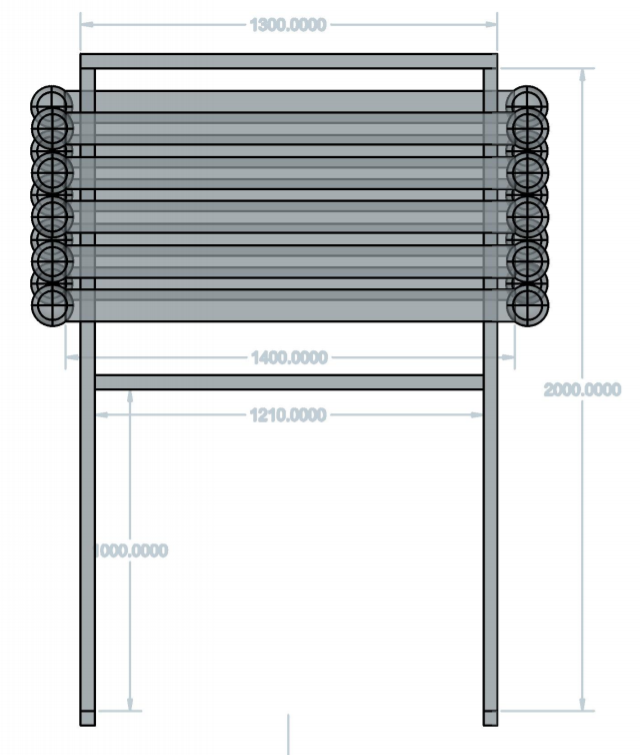
\includegraphics[width=0.6\linewidth]{files/Figures/dstofFront.png}
    		\caption{Front view of the downstream time of flight system}
    		\label{fig:dstofFront}
    	\end{minipage}
    	\hspace{0.3cm}
    	\begin{minipage}[t]{.48\textwidth}
    		\centering
    		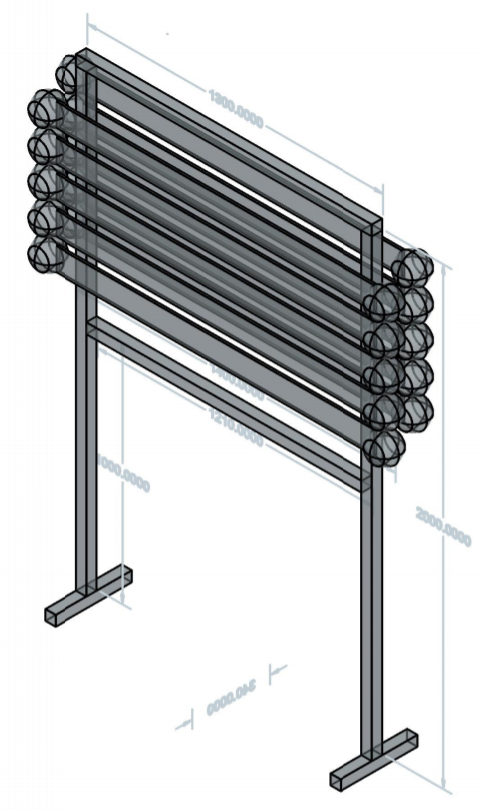
\includegraphics[width=0.45\linewidth]{files/Figures/dstofDiag.png}
    		\caption{Diagonal view of the downstream time of flight system showing more clearly the two rows of scintillator bars and photomultiplier tubes}
    		\label{fig:dstofDiagonal}
    	\end{minipage}
    \end{figure}
    
All 20 of the PMTs have their anode signals read out using NIM discriminators which are then fed into a time-to-digital converter. A signal in S4 was considered to have occurred if a signal was seen in both PMTs on the same bar within 20~ns of each other. 

Additionally, a signal was also fed into the same time-to-digital converter whenever there was a coincidence between the $S1$ and $S2$ timing points. When calculating the time of flight of a given particle, this time of coincidence was used as first timing point.

\subsection{The HPTPC Prototype}
The prototype was built at Royal Holloway, University London.  The steel vessel was rated to 6~barA of pressure, and the walls of the vessel were 4~cm thick (THIS NEEDS CHECKING).
The TPC comprised thin steel mesh electrodes (one cathode and three anodes), and 12 copper rings to create the uniform drift field. The drift distance produced was 48~cm, with the anodes separated by 1~mm. Data taking with the TPC made use of both optical and charge readout.The vessel, electrodes, and drift region of the TPC are shown in figure~\ref{fig:TPC}.
    
     \begin{figure}
      \centering
    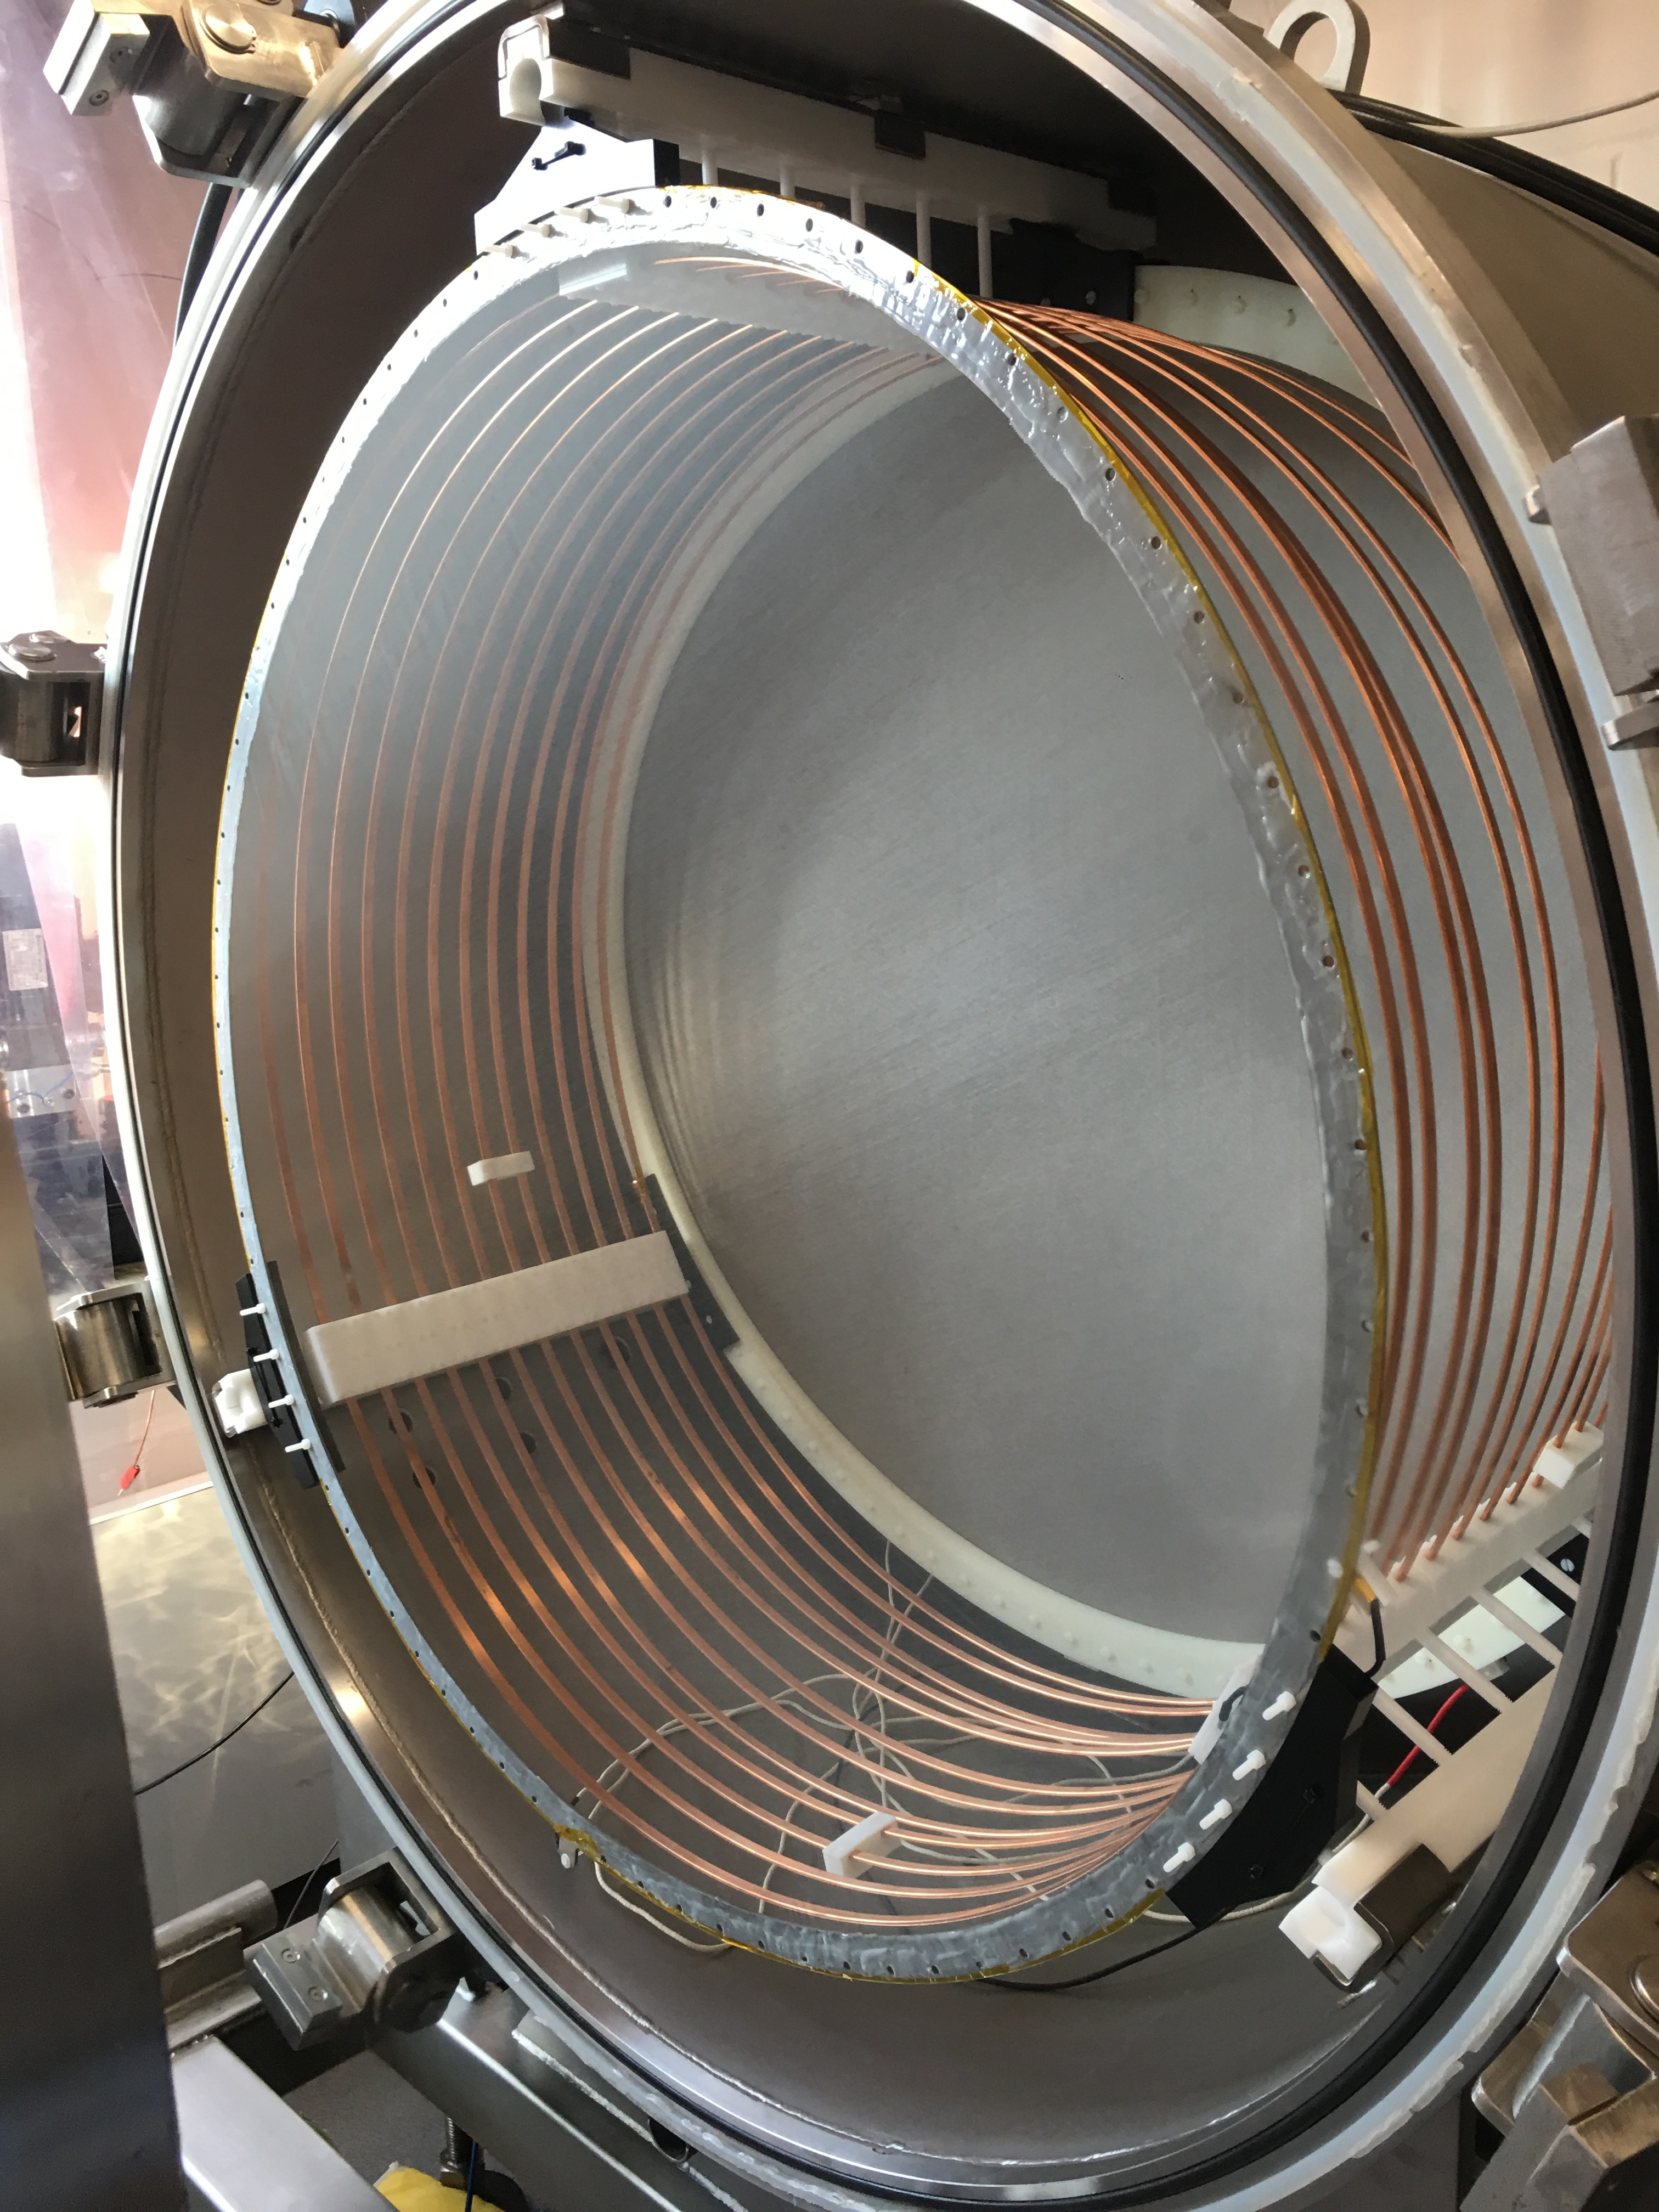
\includegraphics[width=0.6\linewidth]{files/Figures/IMG_1194.jpg}
    	\caption{Cross-sectional view of the TPC; the thing mesh electrodes and copper ring drift volume can be seen inside the steel vessel}
    		\label{fig:TPC}
    \end{figure}
    
The centre of the TPC was placed 13~m from the beam entrance with S3 and S4 directly upstream and downstream of the vessel, respectively. Throughout the run, the TPC was filled with either pure Argon, or a combination of Argon and a small percentage of quencher.


%\subsection{Beam Taking Periods}

%The data taken for the following studies was accrued over the course 
%WHAT DATA AND WHEN (Maybe this goes earlier)
 %(this is described above now)   
\section{Analysis}
\subsection{Analysis Goals}
The primary aims of the use of S1-S4 were to make measurements of the flux of particles entering and exiting the TPC vessel, and to perform particle identification using the time of flight measurement.
Using this data, it is possible to provide a momentum spectrum of particles in- and outgoing from the TPC, and calculate the ratio of particles in the beam.

Protons can be distinguished from particles that are close to minimum ionising (pions, muons, and electrons) which travel the distance from S1 to S3 or S4 in a shorter time.
Distinguishing these MIPs from one another is more difficult (CHECK WITH ALEXANDER K IF WE WANT TO COMMENT ON S3's ABILITY TO DIFFERENTIATE THESE)
From the particle flux data, it is possible to measure the ratio of protons to other particles over the range of off-axis angles covered by the S3 and S4 walls, and for varying numbers of moderator blocks.

The variation of momentum spectrum and proton pion ratio with differing numbers of acrylic blocks off the beam axis provide the motivation for the measurement techniques used.
As such the data used in these results cover two days in the run where the number of moderator blocks were varied with other beam properties held constant.
The number of spills per moderator block configuration were as follows (with more data taken for 4 blocks as that was the configuration used for the majority of the beam test):
0 blocks: 257 spills, 1 block:  254 spills, 2 blocks: 267 spills, 3 blocks: 220 spills, 4 blocks: 3884 spills.


\subsection{Analysis Methods}

	Figure~\ref{fig:s4tof} shows the variation in the time of flight spectrum as recorded by $S4$ with a changing number of moderator blocks.
	This spectrum given by the difference in time between observation of a coincidence in the $S1$ and $S2$ timing points and a signal being recorded in $S4$ (the definition of an $S4$ signal is given above).
	
	\begin{figure}[h]
		\begin{adjustbox}{max totalsize={.8\textwidth}{.5\textheight},center}
			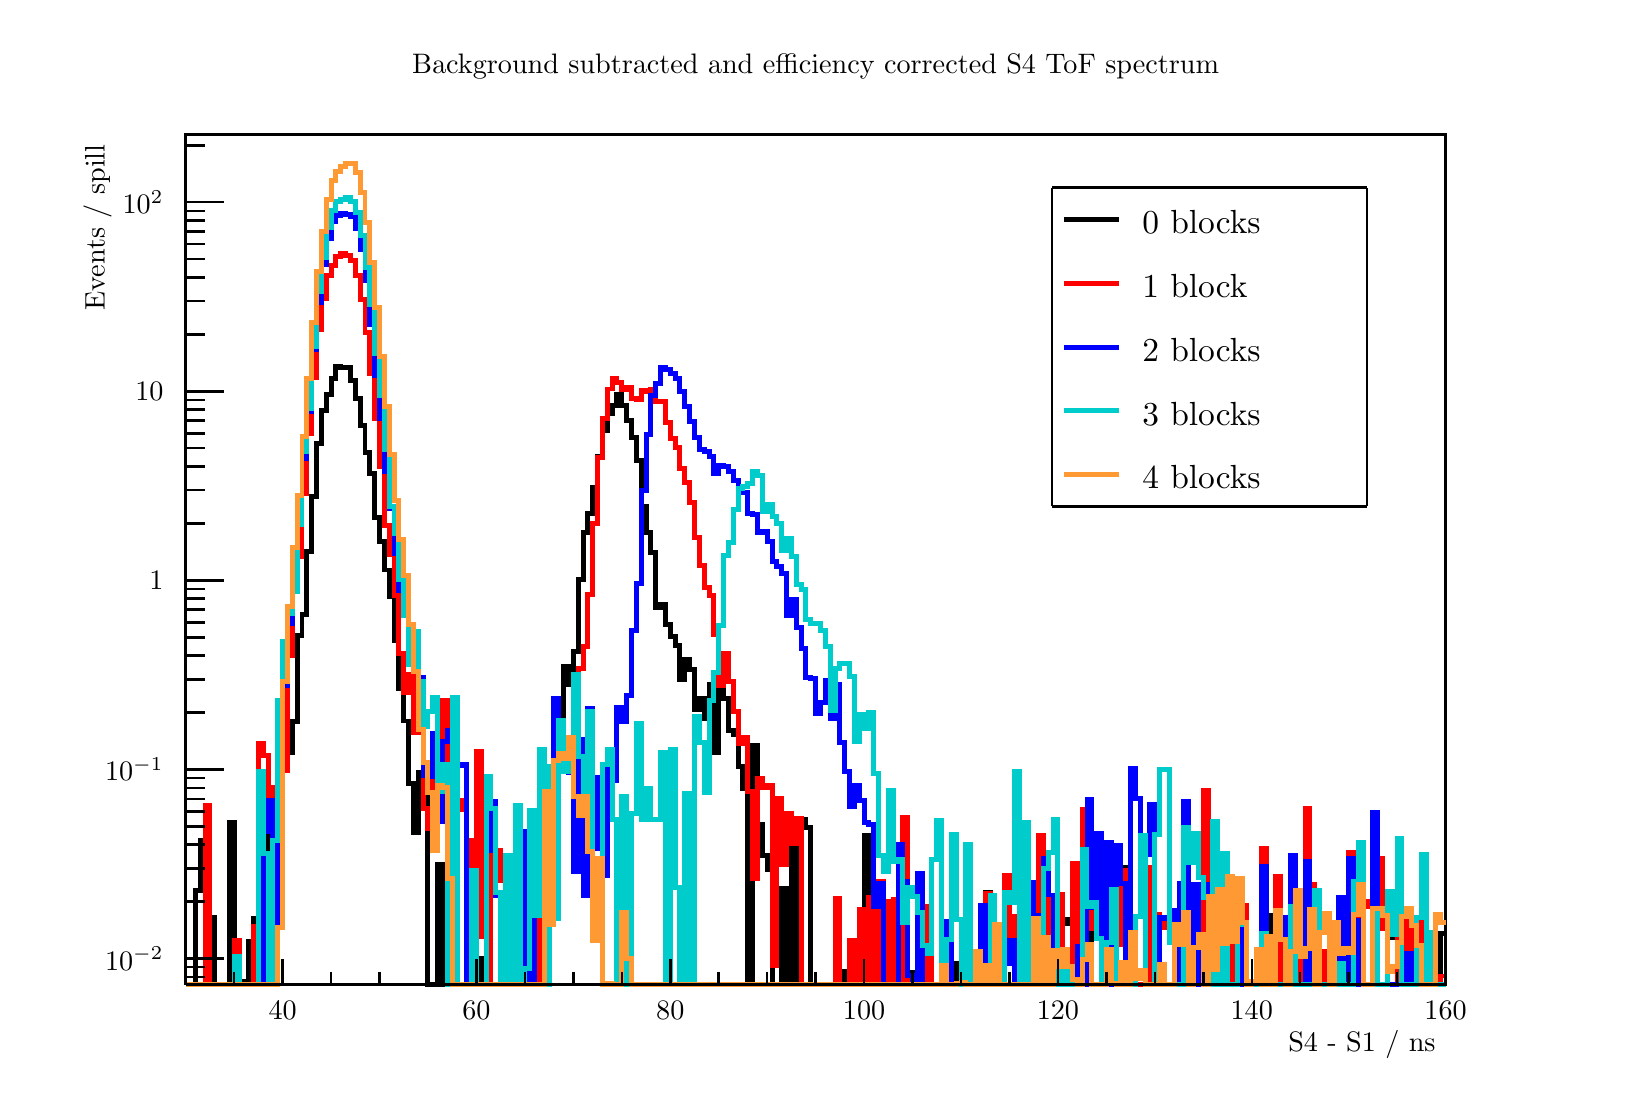
\begin{tikzpicture}
\pgfdeclareplotmark{cross} {
\pgfpathmoveto{\pgfpoint{-0.3\pgfplotmarksize}{\pgfplotmarksize}}
\pgfpathlineto{\pgfpoint{+0.3\pgfplotmarksize}{\pgfplotmarksize}}
\pgfpathlineto{\pgfpoint{+0.3\pgfplotmarksize}{0.3\pgfplotmarksize}}
\pgfpathlineto{\pgfpoint{+1\pgfplotmarksize}{0.3\pgfplotmarksize}}
\pgfpathlineto{\pgfpoint{+1\pgfplotmarksize}{-0.3\pgfplotmarksize}}
\pgfpathlineto{\pgfpoint{+0.3\pgfplotmarksize}{-0.3\pgfplotmarksize}}
\pgfpathlineto{\pgfpoint{+0.3\pgfplotmarksize}{-1.\pgfplotmarksize}}
\pgfpathlineto{\pgfpoint{-0.3\pgfplotmarksize}{-1.\pgfplotmarksize}}
\pgfpathlineto{\pgfpoint{-0.3\pgfplotmarksize}{-0.3\pgfplotmarksize}}
\pgfpathlineto{\pgfpoint{-1.\pgfplotmarksize}{-0.3\pgfplotmarksize}}
\pgfpathlineto{\pgfpoint{-1.\pgfplotmarksize}{0.3\pgfplotmarksize}}
\pgfpathlineto{\pgfpoint{-0.3\pgfplotmarksize}{0.3\pgfplotmarksize}}
\pgfpathclose
\pgfusepathqstroke
}
\pgfdeclareplotmark{cross*} {
\pgfpathmoveto{\pgfpoint{-0.3\pgfplotmarksize}{\pgfplotmarksize}}
\pgfpathlineto{\pgfpoint{+0.3\pgfplotmarksize}{\pgfplotmarksize}}
\pgfpathlineto{\pgfpoint{+0.3\pgfplotmarksize}{0.3\pgfplotmarksize}}
\pgfpathlineto{\pgfpoint{+1\pgfplotmarksize}{0.3\pgfplotmarksize}}
\pgfpathlineto{\pgfpoint{+1\pgfplotmarksize}{-0.3\pgfplotmarksize}}
\pgfpathlineto{\pgfpoint{+0.3\pgfplotmarksize}{-0.3\pgfplotmarksize}}
\pgfpathlineto{\pgfpoint{+0.3\pgfplotmarksize}{-1.\pgfplotmarksize}}
\pgfpathlineto{\pgfpoint{-0.3\pgfplotmarksize}{-1.\pgfplotmarksize}}
\pgfpathlineto{\pgfpoint{-0.3\pgfplotmarksize}{-0.3\pgfplotmarksize}}
\pgfpathlineto{\pgfpoint{-1.\pgfplotmarksize}{-0.3\pgfplotmarksize}}
\pgfpathlineto{\pgfpoint{-1.\pgfplotmarksize}{0.3\pgfplotmarksize}}
\pgfpathlineto{\pgfpoint{-0.3\pgfplotmarksize}{0.3\pgfplotmarksize}}
\pgfpathclose
\pgfusepathqfillstroke
}
\pgfdeclareplotmark{newstar} {
\pgfpathmoveto{\pgfqpoint{0pt}{\pgfplotmarksize}}
\pgfpathlineto{\pgfqpointpolar{44}{0.5\pgfplotmarksize}}
\pgfpathlineto{\pgfqpointpolar{18}{\pgfplotmarksize}}
\pgfpathlineto{\pgfqpointpolar{-20}{0.5\pgfplotmarksize}}
\pgfpathlineto{\pgfqpointpolar{-54}{\pgfplotmarksize}}
\pgfpathlineto{\pgfqpointpolar{-90}{0.5\pgfplotmarksize}}
\pgfpathlineto{\pgfqpointpolar{234}{\pgfplotmarksize}}
\pgfpathlineto{\pgfqpointpolar{198}{0.5\pgfplotmarksize}}
\pgfpathlineto{\pgfqpointpolar{162}{\pgfplotmarksize}}
\pgfpathlineto{\pgfqpointpolar{134}{0.5\pgfplotmarksize}}
\pgfpathclose
\pgfusepathqstroke
}
\pgfdeclareplotmark{newstar*} {
\pgfpathmoveto{\pgfqpoint{0pt}{\pgfplotmarksize}}
\pgfpathlineto{\pgfqpointpolar{44}{0.5\pgfplotmarksize}}
\pgfpathlineto{\pgfqpointpolar{18}{\pgfplotmarksize}}
\pgfpathlineto{\pgfqpointpolar{-20}{0.5\pgfplotmarksize}}
\pgfpathlineto{\pgfqpointpolar{-54}{\pgfplotmarksize}}
\pgfpathlineto{\pgfqpointpolar{-90}{0.5\pgfplotmarksize}}
\pgfpathlineto{\pgfqpointpolar{234}{\pgfplotmarksize}}
\pgfpathlineto{\pgfqpointpolar{198}{0.5\pgfplotmarksize}}
\pgfpathlineto{\pgfqpointpolar{162}{\pgfplotmarksize}}
\pgfpathlineto{\pgfqpointpolar{134}{0.5\pgfplotmarksize}}
\pgfpathclose
\pgfusepathqfillstroke
}
\definecolor{c}{rgb}{1,1,1};
\draw [color=c, fill=c] (0,0) rectangle (20,13.4957);
\draw [color=c, fill=c] (2,1.34957) rectangle (18,12.1461);
\definecolor{c}{rgb}{0,0,0};
\draw [c,line width=0.9] (2,1.34957) -- (2,12.1461) -- (18,12.1461) -- (18,1.34957) -- (2,1.34957);
\definecolor{c}{rgb}{1,1,1};
\draw [color=c, fill=c] (2,1.34957) rectangle (18,12.1461);
\definecolor{c}{rgb}{0,0,0};
\draw [c,line width=0.9] (2,1.34957) -- (2,12.1461) -- (18,12.1461) -- (18,1.34957) -- (2,1.34957);
\definecolor{c}{rgb}{0,0,0.6};
\draw [c,line width=0.9] (2,1.34957) -- (2.06154,1.34957) -- (2.06154,1.34957) -- (2.12308,1.34957) -- (2.12308,1.34957) -- (2.18462,1.34957) -- (2.18462,1.34957) -- (2.24615,1.34957) -- (2.24615,1.34957) -- (2.30769,1.34957) -- (2.30769,1.34957) --
 (2.36923,1.34957) -- (2.36923,1.34957) -- (2.43077,1.34957) -- (2.43077,1.34957) -- (2.49231,1.34957) -- (2.49231,1.34957) -- (2.55385,1.34957) -- (2.55385,1.34957) -- (2.61538,1.34957) -- (2.61538,1.34957) -- (2.67692,1.34957) -- (2.67692,1.34957)
 -- (2.73846,1.34957) -- (2.73846,1.34957) -- (2.8,1.34957) -- (2.8,1.34957) -- (2.86154,1.34957) -- (2.86154,1.34957) -- (2.92308,1.34957) -- (2.92308,1.34957) -- (2.98462,1.34957) -- (2.98462,1.34957) -- (3.04615,1.34957) -- (3.04615,1.34957) --
 (3.10769,1.34957) -- (3.10769,1.34957) -- (3.16923,1.34957) -- (3.16923,1.34957) -- (3.23077,1.34957) -- (3.23077,1.34957) -- (3.29231,1.34957) -- (3.29231,1.34957) -- (3.35385,1.34957) -- (3.35385,1.34957) -- (3.41538,1.34957) -- (3.41538,1.34957)
 -- (3.47692,1.34957) -- (3.47692,1.34957) -- (3.53846,1.34957) -- (3.53846,1.34957) -- (3.6,1.34957) -- (3.6,1.34957) -- (3.66154,1.34957) -- (3.66154,1.34957) -- (3.72308,1.34957) -- (3.72308,1.34957) -- (3.78462,1.34957) -- (3.78462,1.34957) --
 (3.84615,1.34957) -- (3.84615,1.34957) -- (3.90769,1.34957) -- (3.90769,1.34957) -- (3.96923,1.34957) -- (3.96923,1.34957) -- (4.03077,1.34957) -- (4.03077,1.34957) -- (4.09231,1.34957) -- (4.09231,1.34957) -- (4.15385,1.34957) -- (4.15385,1.34957)
 -- (4.21538,1.34957) -- (4.21538,1.34957) -- (4.27692,1.34957) -- (4.27692,1.34957) -- (4.33846,1.34957) -- (4.33846,1.34957) -- (4.4,1.34957) -- (4.4,1.34957) -- (4.46154,1.34957) -- (4.46154,1.34957) -- (4.52308,1.34957) -- (4.52308,1.34957) --
 (4.58462,1.34957) -- (4.58462,1.34957) -- (4.64615,1.34957) -- (4.64615,1.34957) -- (4.70769,1.34957) -- (4.70769,1.34957) -- (4.76923,1.34957) -- (4.76923,1.34957) -- (4.83077,1.34957) -- (4.83077,1.34957) -- (4.89231,1.34957) -- (4.89231,1.34957)
 -- (4.95385,1.34957) -- (4.95385,1.34957) -- (5.01538,1.34957) -- (5.01538,1.34957) -- (5.07692,1.34957) -- (5.07692,1.34957) -- (5.13846,1.34957) -- (5.13846,1.34957) -- (5.2,1.34957) -- (5.2,1.34957) -- (5.26154,1.34957) -- (5.26154,1.34957) --
 (5.32308,1.34957) -- (5.32308,1.34957) -- (5.38462,1.34957) -- (5.38462,1.34957) -- (5.44615,1.34957) -- (5.44615,1.34957) -- (5.50769,1.34957) -- (5.50769,1.34957) -- (5.56923,1.34957) -- (5.56923,1.34957) -- (5.63077,1.34957) -- (5.63077,1.34957)
 -- (5.69231,1.34957) -- (5.69231,1.34957) -- (5.75385,1.34957) -- (5.75385,1.34957) -- (5.81538,1.34957) -- (5.81538,1.34957) -- (5.87692,1.34957) -- (5.87692,1.34957) -- (5.93846,1.34957) -- (5.93846,1.34957) -- (6,1.34957) -- (6,1.34957) --
 (6.06154,1.34957) -- (6.06154,1.34957) -- (6.12308,1.34957) -- (6.12308,1.34957) -- (6.18462,1.34957) -- (6.18462,1.34957) -- (6.24615,1.34957) -- (6.24615,1.34957) -- (6.30769,1.34957) -- (6.30769,1.34957) -- (6.36923,1.34957) -- (6.36923,1.34957)
 -- (6.43077,1.34957) -- (6.43077,1.34957) -- (6.49231,1.34957) -- (6.49231,1.34957) -- (6.55385,1.34957) -- (6.55385,1.34957) -- (6.61538,1.34957) -- (6.61538,1.34957) -- (6.67692,1.34957) -- (6.67692,1.34957) -- (6.73846,1.34957) --
 (6.73846,1.34957) -- (6.8,1.34957) -- (6.8,1.34957) -- (6.86154,1.34957) -- (6.86154,1.34957) -- (6.92308,1.34957) -- (6.92308,1.34957) -- (6.98462,1.34957) -- (6.98462,1.34957) -- (7.04615,1.34957) -- (7.04615,1.34957) -- (7.10769,1.34957) --
 (7.10769,1.34957) -- (7.16923,1.34957) -- (7.16923,1.34957) -- (7.23077,1.34957) -- (7.23077,1.34957) -- (7.29231,1.34957) -- (7.29231,1.34957) -- (7.35385,1.34957) -- (7.35385,1.34957) -- (7.41538,1.34957) -- (7.41538,1.34957) -- (7.47692,1.34957)
 -- (7.47692,1.34957) -- (7.53846,1.34957) -- (7.53846,1.34957) -- (7.6,1.34957) -- (7.6,1.34957) -- (7.66154,1.34957) -- (7.66154,1.34957) -- (7.72308,1.34957) -- (7.72308,1.34957) -- (7.78462,1.34957) -- (7.78462,1.34957) -- (7.84615,1.34957) --
 (7.84615,1.34957) -- (7.90769,1.34957) -- (7.90769,1.34957) -- (7.96923,1.34957) -- (7.96923,1.34957) -- (8.03077,1.34957) -- (8.03077,1.34957) -- (8.09231,1.34957) -- (8.09231,1.34957) -- (8.15385,1.34957) -- (8.15385,1.34957) -- (8.21538,1.34957)
 -- (8.21538,1.34957) -- (8.27692,1.34957) -- (8.27692,1.34957) -- (8.33846,1.34957) -- (8.33846,1.34957) -- (8.4,1.34957) -- (8.4,1.34957) -- (8.46154,1.34957) -- (8.46154,1.34957) -- (8.52308,1.34957) -- (8.52308,1.34957) -- (8.58462,1.34957) --
 (8.58462,1.34957) -- (8.64615,1.34957) -- (8.64615,1.34957) -- (8.70769,1.34957) -- (8.70769,1.34957) -- (8.76923,1.34957) -- (8.76923,1.34957) -- (8.83077,1.34957) -- (8.83077,1.34957) -- (8.89231,1.34957) -- (8.89231,1.34957) -- (8.95385,1.34957)
 -- (8.95385,1.34957) -- (9.01538,1.34957) -- (9.01538,1.34957) -- (9.07692,1.34957) -- (9.07692,1.34957) -- (9.13846,1.34957) -- (9.13846,1.34957) -- (9.2,1.34957) -- (9.2,1.34957) -- (9.26154,1.34957) -- (9.26154,1.34957) -- (9.32308,1.34957) --
 (9.32308,1.34957) -- (9.38461,1.34957) -- (9.38461,1.34957) -- (9.44615,1.34957) -- (9.44615,1.34957) -- (9.50769,1.34957) -- (9.50769,1.34957) -- (9.56923,1.34957) -- (9.56923,1.34957) -- (9.63077,1.34957) -- (9.63077,1.34957) -- (9.69231,1.34957)
 -- (9.69231,1.34957) -- (9.75385,1.34957) -- (9.75385,1.34957) -- (9.81538,1.34957) -- (9.81538,1.34957) -- (9.87692,1.34957) -- (9.87692,1.34957) -- (9.93846,1.34957) -- (9.93846,1.34957) -- (10,1.34957) -- (10,1.34957) -- (10.0615,1.34957) --
 (10.0615,1.34957) -- (10.1231,1.34957) -- (10.1231,1.34957) -- (10.1846,1.34957) -- (10.1846,1.34957) -- (10.2462,1.34957) -- (10.2462,1.34957) -- (10.3077,1.34957) -- (10.3077,1.34957) -- (10.3692,1.34957) -- (10.3692,1.34957) -- (10.4308,1.34957)
 -- (10.4308,1.34957) -- (10.4923,1.34957) -- (10.4923,1.34957) -- (10.5538,1.34957) -- (10.5538,1.34957) -- (10.6154,1.34957) -- (10.6154,1.34957) -- (10.6769,1.34957) -- (10.6769,1.34957) -- (10.7385,1.34957) -- (10.7385,1.34957) -- (10.8,1.34957)
 -- (10.8,1.34957) -- (10.8615,1.34957) -- (10.8615,1.34957) -- (10.9231,1.34957) -- (10.9231,1.34957) -- (10.9846,1.34957) -- (10.9846,1.34957) -- (11.0462,1.34957) -- (11.0462,1.34957) -- (11.1077,1.34957) -- (11.1077,1.34957) -- (11.1692,1.34957)
 -- (11.1692,1.34957) -- (11.2308,1.34957) -- (11.2308,1.34957) -- (11.2923,1.34957) -- (11.2923,1.34957) -- (11.3538,1.34957) -- (11.3538,1.34957) -- (11.4154,1.34957) -- (11.4154,1.34957) -- (11.4769,1.34957) -- (11.4769,1.34957) --
 (11.5385,1.34957) -- (11.5385,1.34957) -- (11.6,1.34957) -- (11.6,1.34957) -- (11.6615,1.34957) -- (11.6615,1.34957) -- (11.7231,1.34957) -- (11.7231,1.34957) -- (11.7846,1.34957) -- (11.7846,1.34957) -- (11.8462,1.34957) -- (11.8462,1.34957) --
 (11.9077,1.34957) -- (11.9077,1.34957) -- (11.9692,1.34957) -- (11.9692,1.34957) -- (12.0308,1.34957) -- (12.0308,1.34957) -- (12.0923,1.34957) -- (12.0923,1.34957) -- (12.1538,1.34957) -- (12.1538,1.34957) -- (12.2154,1.34957) -- (12.2154,1.34957)
 -- (12.2769,1.34957) -- (12.2769,1.34957) -- (12.3385,1.34957) -- (12.3385,1.34957) -- (12.4,1.34957) -- (12.4,1.34957) -- (12.4615,1.34957) -- (12.4615,1.34957) -- (12.5231,1.34957) -- (12.5231,1.34957) -- (12.5846,1.34957) -- (12.5846,1.34957) --
 (12.6462,1.34957) -- (12.6462,1.34957) -- (12.7077,1.34957) -- (12.7077,1.34957) -- (12.7692,1.34957) -- (12.7692,1.34957) -- (12.8308,1.34957) -- (12.8308,1.34957) -- (12.8923,1.34957) -- (12.8923,1.34957) -- (12.9538,1.34957) -- (12.9538,1.34957)
 -- (13.0154,1.34957) -- (13.0154,1.34957) -- (13.0769,1.34957) -- (13.0769,1.34957) -- (13.1385,1.34957) -- (13.1385,1.34957) -- (13.2,1.34957) -- (13.2,1.34957) -- (13.2615,1.34957) -- (13.2615,1.34957) -- (13.3231,1.34957) -- (13.3231,1.34957) --
 (13.3846,1.34957) -- (13.3846,1.34957) -- (13.4462,1.34957) -- (13.4462,1.34957) -- (13.5077,1.34957) -- (13.5077,1.34957) -- (13.5692,1.34957) -- (13.5692,1.34957) -- (13.6308,1.34957) -- (13.6308,1.34957) -- (13.6923,1.34957) -- (13.6923,1.34957)
 -- (13.7538,1.34957) -- (13.7538,1.34957) -- (13.8154,1.34957) -- (13.8154,1.34957) -- (13.8769,1.34957) -- (13.8769,1.34957) -- (13.9385,1.34957) -- (13.9385,1.34957) -- (14,1.34957) -- (14,1.34957) -- (14.0615,1.34957) -- (14.0615,1.34957) --
 (14.1231,1.34957) -- (14.1231,1.34957) -- (14.1846,1.34957) -- (14.1846,1.34957) -- (14.2462,1.34957) -- (14.2462,1.34957) -- (14.3077,1.34957) -- (14.3077,1.34957) -- (14.3692,1.34957) -- (14.3692,1.34957) -- (14.4308,1.34957) -- (14.4308,1.34957)
 -- (14.4923,1.34957) -- (14.4923,1.34957) -- (14.5538,1.34957) -- (14.5538,1.34957) -- (14.6154,1.34957) -- (14.6154,1.34957) -- (14.6769,1.34957) -- (14.6769,1.34957) -- (14.7385,1.34957) -- (14.7385,1.34957) -- (14.8,1.34957) -- (14.8,1.34957) --
 (14.8615,1.34957) -- (14.8615,1.34957) -- (14.9231,1.34957) -- (14.9231,1.34957) -- (14.9846,1.34957) -- (14.9846,1.34957) -- (15.0462,1.34957) -- (15.0462,1.34957) -- (15.1077,1.34957) -- (15.1077,1.34957) -- (15.1692,1.34957) -- (15.1692,1.34957)
 -- (15.2308,1.34957) -- (15.2308,1.34957) -- (15.2923,1.34957) -- (15.2923,1.34957) -- (15.3538,1.34957) -- (15.3538,1.34957) -- (15.4154,1.34957) -- (15.4154,1.34957) -- (15.4769,1.34957) -- (15.4769,1.34957) -- (15.5385,1.34957) --
 (15.5385,1.34957) -- (15.6,1.34957) -- (15.6,1.34957) -- (15.6615,1.34957) -- (15.6615,1.34957) -- (15.7231,1.34957) -- (15.7231,1.34957) -- (15.7846,1.34957) -- (15.7846,1.34957) -- (15.8462,1.34957) -- (15.8462,1.34957) -- (15.9077,1.34957) --
 (15.9077,1.34957) -- (15.9692,1.34957) -- (15.9692,1.34957) -- (16.0308,1.34957) -- (16.0308,1.34957) -- (16.0923,1.34957) -- (16.0923,1.34957) -- (16.1538,1.34957) -- (16.1538,1.34957) -- (16.2154,1.34957) -- (16.2154,1.34957) -- (16.2769,1.34957)
 -- (16.2769,1.34957) -- (16.3385,1.34957) -- (16.3385,1.34957) -- (16.4,1.34957) -- (16.4,1.34957) -- (16.4615,1.34957) -- (16.4615,1.34957) -- (16.5231,1.34957) -- (16.5231,1.34957) -- (16.5846,1.34957) -- (16.5846,1.34957) -- (16.6462,1.34957) --
 (16.6462,1.34957) -- (16.7077,1.34957) -- (16.7077,1.34957) -- (16.7692,1.34957) -- (16.7692,1.34957) -- (16.8308,1.34957) -- (16.8308,1.34957) -- (16.8923,1.34957) -- (16.8923,1.34957) -- (16.9538,1.34957) -- (16.9538,1.34957) -- (17.0154,1.34957)
 -- (17.0154,1.34957) -- (17.0769,1.34957) -- (17.0769,1.34957) -- (17.1385,1.34957) -- (17.1385,1.34957) -- (17.2,1.34957) -- (17.2,1.34957) -- (17.2615,1.34957) -- (17.2615,1.34957) -- (17.3231,1.34957) -- (17.3231,1.34957) -- (17.3846,1.34957) --
 (17.3846,1.34957) -- (17.4462,1.34957) -- (17.4462,1.34957) -- (17.5077,1.34957) -- (17.5077,1.34957) -- (17.5692,1.34957) -- (17.5692,1.34957) -- (17.6308,1.34957) -- (17.6308,1.34957) -- (17.6923,1.34957) -- (17.6923,1.34957) -- (17.7538,1.34957)
 -- (17.7538,1.34957) -- (17.8154,1.34957) -- (17.8154,1.34957) -- (17.8769,1.34957) -- (17.8769,1.34957) -- (17.9385,1.34957) -- (17.9385,1.34957) -- (18,1.34957);
\definecolor{c}{rgb}{0,0,0};
\draw [c,line width=0.9] (2,1.34957) -- (18,1.34957);
\draw [c,line width=0.9] (3.23077,1.67347) -- (3.23077,1.34957);
\draw [c,line width=0.9] (3.84615,1.51152) -- (3.84615,1.34957);
\draw [c,line width=0.9] (4.46154,1.51152) -- (4.46154,1.34957);
\draw [c,line width=0.9] (5.07692,1.51152) -- (5.07692,1.34957);
\draw [c,line width=0.9] (5.69231,1.67347) -- (5.69231,1.34957);
\draw [c,line width=0.9] (6.30769,1.51152) -- (6.30769,1.34957);
\draw [c,line width=0.9] (6.92308,1.51152) -- (6.92308,1.34957);
\draw [c,line width=0.9] (7.53846,1.51152) -- (7.53846,1.34957);
\draw [c,line width=0.9] (8.15385,1.67347) -- (8.15385,1.34957);
\draw [c,line width=0.9] (8.76923,1.51152) -- (8.76923,1.34957);
\draw [c,line width=0.9] (9.38461,1.51152) -- (9.38461,1.34957);
\draw [c,line width=0.9] (10,1.51152) -- (10,1.34957);
\draw [c,line width=0.9] (10.6154,1.67347) -- (10.6154,1.34957);
\draw [c,line width=0.9] (11.2308,1.51152) -- (11.2308,1.34957);
\draw [c,line width=0.9] (11.8462,1.51152) -- (11.8462,1.34957);
\draw [c,line width=0.9] (12.4615,1.51152) -- (12.4615,1.34957);
\draw [c,line width=0.9] (13.0769,1.67347) -- (13.0769,1.34957);
\draw [c,line width=0.9] (13.6923,1.51152) -- (13.6923,1.34957);
\draw [c,line width=0.9] (14.3077,1.51152) -- (14.3077,1.34957);
\draw [c,line width=0.9] (14.9231,1.51152) -- (14.9231,1.34957);
\draw [c,line width=0.9] (15.5385,1.67347) -- (15.5385,1.34957);
\draw [c,line width=0.9] (16.1538,1.51152) -- (16.1538,1.34957);
\draw [c,line width=0.9] (16.7692,1.51152) -- (16.7692,1.34957);
\draw [c,line width=0.9] (17.3846,1.51152) -- (17.3846,1.34957);
\draw [c,line width=0.9] (18,1.67347) -- (18,1.34957);
\draw [c,line width=0.9] (3.23077,1.67347) -- (3.23077,1.34957);
\draw [c,line width=0.9] (2.61538,1.51152) -- (2.61538,1.34957);
\draw [c,line width=0.9] (2,1.51152) -- (2,1.34957);
\draw [anchor=base] (3.23077,0.904212) node[scale=1.01821, color=c, rotate=0]{40};
\draw [anchor=base] (5.69231,0.904212) node[scale=1.01821, color=c, rotate=0]{60};
\draw [anchor=base] (8.15385,0.904212) node[scale=1.01821, color=c, rotate=0]{80};
\draw [anchor=base] (10.6154,0.904212) node[scale=1.01821, color=c, rotate=0]{100};
\draw [anchor=base] (13.0769,0.904212) node[scale=1.01821, color=c, rotate=0]{120};
\draw [anchor=base] (15.5385,0.904212) node[scale=1.01821, color=c, rotate=0]{140};
\draw [anchor=base] (18,0.904212) node[scale=1.01821, color=c, rotate=0]{160};
\draw [anchor= east] (18,0.593811) node[scale=1.01821, color=c, rotate=0]{ S4 - S1 / ns};
\draw [c,line width=0.9] (2,1.34957) -- (2,12.1461);
\draw [c,line width=0.9] (2.24,1.44788) -- (2,1.44788);
\draw [c,line width=0.9] (2.24,1.57071) -- (2,1.57071);
\draw [c,line width=0.9] (2.48,1.68059) -- (2,1.68059);
\draw [anchor= east] (1.844,1.68059) node[scale=1.01821, color=c, rotate=0]{$10^{-2}$};
\draw [c,line width=0.9] (2.24,2.40344) -- (2,2.40344);
\draw [c,line width=0.9] (2.24,2.82629) -- (2,2.82629);
\draw [c,line width=0.9] (2.24,3.1263) -- (2,3.1263);
\draw [c,line width=0.9] (2.24,3.35901) -- (2,3.35901);
\draw [c,line width=0.9] (2.24,3.54914) -- (2,3.54914);
\draw [c,line width=0.9] (2.24,3.7099) -- (2,3.7099);
\draw [c,line width=0.9] (2.24,3.84916) -- (2,3.84916);
\draw [c,line width=0.9] (2.24,3.97199) -- (2,3.97199);
\draw [c,line width=0.9] (2.48,4.08186) -- (2,4.08186);
\draw [anchor= east] (1.844,4.08186) node[scale=1.01821, color=c, rotate=0]{$10^{-1}$};
\draw [c,line width=0.9] (2.24,4.80472) -- (2,4.80472);
\draw [c,line width=0.9] (2.24,5.22756) -- (2,5.22756);
\draw [c,line width=0.9] (2.24,5.52758) -- (2,5.52758);
\draw [c,line width=0.9] (2.24,5.76028) -- (2,5.76028);
\draw [c,line width=0.9] (2.24,5.95042) -- (2,5.95042);
\draw [c,line width=0.9] (2.24,6.11118) -- (2,6.11118);
\draw [c,line width=0.9] (2.24,6.25043) -- (2,6.25043);
\draw [c,line width=0.9] (2.24,6.37327) -- (2,6.37327);
\draw [c,line width=0.9] (2.48,6.48314) -- (2,6.48314);
\draw [anchor= east] (1.844,6.48314) node[scale=1.01821, color=c, rotate=0]{1};
\draw [c,line width=0.9] (2.24,7.206) -- (2,7.206);
\draw [c,line width=0.9] (2.24,7.62884) -- (2,7.62884);
\draw [c,line width=0.9] (2.24,7.92885) -- (2,7.92885);
\draw [c,line width=0.9] (2.24,8.16156) -- (2,8.16156);
\draw [c,line width=0.9] (2.24,8.3517) -- (2,8.3517);
\draw [c,line width=0.9] (2.24,8.51246) -- (2,8.51246);
\draw [c,line width=0.9] (2.24,8.65171) -- (2,8.65171);
\draw [c,line width=0.9] (2.24,8.77454) -- (2,8.77454);
\draw [c,line width=0.9] (2.48,8.88442) -- (2,8.88442);
\draw [anchor= east] (1.844,8.88442) node[scale=1.01821, color=c, rotate=0]{10};
\draw [c,line width=0.9] (2.24,9.60728) -- (2,9.60728);
\draw [c,line width=0.9] (2.24,10.0301) -- (2,10.0301);
\draw [c,line width=0.9] (2.24,10.3301) -- (2,10.3301);
\draw [c,line width=0.9] (2.24,10.5628) -- (2,10.5628);
\draw [c,line width=0.9] (2.24,10.753) -- (2,10.753);
\draw [c,line width=0.9] (2.24,10.9137) -- (2,10.9137);
\draw [c,line width=0.9] (2.24,11.053) -- (2,11.053);
\draw [c,line width=0.9] (2.24,11.1758) -- (2,11.1758);
\draw [c,line width=0.9] (2.48,11.2857) -- (2,11.2857);
\draw [anchor= east] (1.844,11.2857) node[scale=1.01821, color=c, rotate=0]{$10^{2}$};
\draw [c,line width=0.9] (2.24,12.0086) -- (2,12.0086);
\draw [anchor= east] (0.88,12.1461) node[scale=1.01821, color=c, rotate=90]{ Events / spill};
\draw [c,line width=1.8] (2,1.34957) -- (2.06154,1.34957) -- (2.06154,1.34957) -- (2.12308,1.34957) -- (2.12308,2.53951) -- (2.18462,2.53951) -- (2.18462,3.17729) -- (2.24615,3.17729) -- (2.24615,1.34957) -- (2.30769,1.34957) -- (2.30769,2.20144) --
 (2.36923,2.20144) -- (2.36923,1.34957) -- (2.43077,1.34957) -- (2.43077,1.34957) -- (2.49231,1.34957) -- (2.49231,1.34957) -- (2.55385,1.34957) -- (2.55385,3.40479) -- (2.61538,3.40479) -- (2.61538,1.34957) -- (2.67692,1.34957) -- (2.67692,1.34957)
 -- (2.73846,1.34957) -- (2.73846,1.38687) -- (2.8,1.38687) -- (2.8,1.90133) -- (2.86154,1.90133) -- (2.86154,2.18515) -- (2.92308,2.18515) -- (2.92308,3.61789) -- (2.98462,3.61789) -- (2.98462,3.25403) -- (3.04615,3.25403) -- (3.04615,1.34957) --
 (3.10769,1.34957) -- (3.10769,3.39189) -- (3.16923,3.39189) -- (3.16923,4.13184) -- (3.23077,4.13184) -- (3.23077,4.44884) -- (3.29231,4.44884) -- (3.29231,4.30025) -- (3.35385,4.30025) -- (3.35385,4.68859) -- (3.41538,4.68859) -- (3.41538,5.78092)
 -- (3.47692,5.78092) -- (3.47692,6.05252) -- (3.53846,6.05252) -- (3.53846,6.85477) -- (3.6,6.85477) -- (3.6,7.55269) -- (3.66154,7.55269) -- (3.66154,8.22225) -- (3.72308,8.22225) -- (3.72308,8.64481) -- (3.78462,8.64481) -- (3.78462,8.84179) --
 (3.84615,8.84179) -- (3.84615,9.04392) -- (3.90769,9.04392) -- (3.90769,9.20268) -- (3.96923,9.20268) -- (3.96923,9.18123) -- (4.03077,9.18123) -- (4.03077,9.19048) -- (4.09231,9.19048) -- (4.09231,9.02681) -- (4.15385,9.02681) -- (4.15385,8.78913)
 -- (4.21538,8.78913) -- (4.21538,8.45125) -- (4.27692,8.45125) -- (4.27692,8.10572) -- (4.33846,8.10572) -- (4.33846,7.84076) -- (4.4,7.84076) -- (4.4,7.28435) -- (4.46154,7.28435) -- (4.46154,6.98214) -- (4.52308,6.98214) -- (4.52308,6.61504) --
 (4.58462,6.61504) -- (4.58462,6.27553) -- (4.64615,6.27553) -- (4.64615,5.72202) -- (4.70769,5.72202) -- (4.70769,5.11195) -- (4.76923,5.11195) -- (4.76923,4.69735) -- (4.83077,4.69735) -- (4.83077,3.90316) -- (4.89231,3.90316) -- (4.89231,3.28257)
 -- (4.95385,3.28257) -- (4.95385,4.04247) -- (5.01538,4.04247) -- (5.01538,3.738) -- (5.07692,3.738) -- (5.07692,1.34957) -- (5.13846,1.34957) -- (5.13846,1.34957) -- (5.2,1.34957) -- (5.2,2.87862) -- (5.26154,2.87862) -- (5.26154,1.34957) --
 (5.32308,1.34957) -- (5.32308,2.92743) -- (5.38462,2.92743) -- (5.38462,3.00257) -- (5.44615,3.00257) -- (5.44615,1.34957) -- (5.50769,1.34957) -- (5.50769,1.34957) -- (5.56923,1.34957) -- (5.56923,1.34957) -- (5.63077,1.34957) -- (5.63077,1.34957)
 -- (5.69231,1.34957) -- (5.69231,1.68015) -- (5.75385,1.68015) -- (5.75385,1.34957) -- (5.81538,1.34957) -- (5.81538,2.57343) -- (5.87692,2.57343) -- (5.87692,1.34957) -- (5.93846,1.34957) -- (5.93846,1.34957) -- (6,1.34957) -- (6,1.34957) --
 (6.06154,1.34957) -- (6.06154,1.34957) -- (6.12308,1.34957) -- (6.12308,1.34957) -- (6.18462,1.34957) -- (6.18462,1.34957) -- (6.24615,1.34957) -- (6.24615,2.06003) -- (6.30769,2.06003) -- (6.30769,1.34957) -- (6.36923,1.34957) -- (6.36923,1.34957)
 -- (6.43077,1.34957) -- (6.43077,3.20391) -- (6.49231,3.20391) -- (6.49231,2.17723) -- (6.55385,2.17723) -- (6.55385,3.12456) -- (6.61538,3.12456) -- (6.61538,3.55551) -- (6.67692,3.55551) -- (6.67692,4.3017) -- (6.73846,4.3017) -- (6.73846,4.53853)
 -- (6.8,4.53853) -- (6.8,5.38926) -- (6.86154,5.38926) -- (6.86154,5.16006) -- (6.92308,5.16006) -- (6.92308,5.57801) -- (6.98462,5.57801) -- (6.98462,6.49955) -- (7.04615,6.49955) -- (7.04615,7.08983) -- (7.10769,7.08983) -- (7.10769,7.32942) --
 (7.16923,7.32942) -- (7.16923,7.66242) -- (7.23077,7.66242) -- (7.23077,8.06249) -- (7.29231,8.06249) -- (7.29231,8.38303) -- (7.35385,8.38303) -- (7.35385,8.60368) -- (7.41538,8.60368) -- (7.41538,8.70027) -- (7.47692,8.70027) -- (7.47692,8.84394)
 -- (7.53846,8.84394) -- (7.53846,8.70221) -- (7.6,8.70221) -- (7.6,8.51775) -- (7.66154,8.51775) -- (7.66154,8.29905) -- (7.72308,8.29905) -- (7.72308,8.00204) -- (7.78462,8.00204) -- (7.78462,7.42284) -- (7.84615,7.42284) -- (7.84615,7.09375) --
 (7.90769,7.09375) -- (7.90769,6.83915) -- (7.96923,6.83915) -- (7.96923,6.1409) -- (8.03077,6.1409) -- (8.03077,6.18103) -- (8.09231,6.18103) -- (8.09231,5.92597) -- (8.15385,5.92597) -- (8.15385,5.76712) -- (8.21538,5.76712) -- (8.21538,5.6565) --
 (8.27692,5.6565) -- (8.27692,5.2214) -- (8.33846,5.2214) -- (8.33846,5.48398) -- (8.4,5.48398) -- (8.4,5.35061) -- (8.46154,5.35061) -- (8.46154,4.83908) -- (8.52308,4.83908) -- (8.52308,4.97696) -- (8.58462,4.97696) -- (8.58462,4.72547) --
 (8.64615,4.72547) -- (8.64615,5.16273) -- (8.70769,5.16273) -- (8.70769,4.30101) -- (8.76923,4.30101) -- (8.76923,5.1798) -- (8.83077,5.1798) -- (8.83077,4.98008) -- (8.89231,4.98008) -- (8.89231,4.57223) -- (8.95385,4.57223) -- (8.95385,4.52429) --
 (9.01538,4.52429) -- (9.01538,4.11848) -- (9.07692,4.11848) -- (9.07692,3.84027) -- (9.13846,3.84027) -- (9.13846,1.34957) -- (9.2,1.34957) -- (9.2,4.38175) -- (9.26154,4.38175) -- (9.26154,3.37945) -- (9.32308,3.37945) -- (9.32308,2.98425) --
 (9.38461,2.98425) -- (9.38461,2.81682) -- (9.44615,2.81682) -- (9.44615,1.34957) -- (9.50769,1.34957) -- (9.50769,1.34957) -- (9.56923,1.34957) -- (9.56923,2.56799) -- (9.63077,2.56799) -- (9.63077,1.34957) -- (9.69231,1.34957) -- (9.69231,3.38931)
 -- (9.75385,3.38931) -- (9.75385,1.34957) -- (9.81538,1.34957) -- (9.81538,3.44534) -- (9.87692,3.44534) -- (9.87692,3.34676) -- (9.93846,3.34676) -- (9.93846,1.34957) -- (10,1.34957) -- (10,1.34957) -- (10.0615,1.34957) -- (10.0615,1.34957) --
 (10.1231,1.34957) -- (10.1231,1.34957) -- (10.1846,1.34957) -- (10.1846,1.34957) -- (10.2462,1.34957) -- (10.2462,1.34957) -- (10.3077,1.34957) -- (10.3077,1.51017) -- (10.3692,1.51017) -- (10.3692,1.34957) -- (10.4308,1.34957) -- (10.4308,1.34957)
 -- (10.4923,1.34957) -- (10.4923,1.34957) -- (10.5538,1.34957) -- (10.5538,1.34957) -- (10.6154,1.34957) -- (10.6154,3.2483) -- (10.6769,3.2483) -- (10.6769,1.77041) -- (10.7385,1.77041) -- (10.7385,1.34957) -- (10.8,1.34957) -- (10.8,1.34957) --
 (10.8615,1.34957) -- (10.8615,1.34957) -- (10.9231,1.34957) -- (10.9231,1.34957) -- (10.9846,1.34957) -- (10.9846,1.34957) -- (11.0462,1.34957) -- (11.0462,1.34957) -- (11.1077,1.34957) -- (11.1077,1.34957) -- (11.1692,1.34957) -- (11.1692,1.49969)
 -- (11.2308,1.49969) -- (11.2308,1.34957) -- (11.2923,1.34957) -- (11.2923,1.34957) -- (11.3538,1.34957) -- (11.3538,1.34957) -- (11.4154,1.34957) -- (11.4154,1.34957) -- (11.4769,1.34957) -- (11.4769,1.34957) -- (11.5385,1.34957) --
 (11.5385,1.34957) -- (11.6,1.34957) -- (11.6,1.34957) -- (11.6615,1.34957) -- (11.6615,1.85741) -- (11.7231,1.85741) -- (11.7231,1.34957) -- (11.7846,1.34957) -- (11.7846,1.62176) -- (11.8462,1.62176) -- (11.8462,1.34957) -- (11.9077,1.34957) --
 (11.9077,1.34957) -- (11.9692,1.34957) -- (11.9692,1.35861) -- (12.0308,1.35861) -- (12.0308,1.34957) -- (12.0923,1.34957) -- (12.0923,1.34957) -- (12.1538,1.34957) -- (12.1538,2.52198) -- (12.2154,2.52198) -- (12.2154,1.34957) -- (12.2769,1.34957)
 -- (12.2769,1.34957) -- (12.3385,1.34957) -- (12.3385,1.34957) -- (12.4,1.34957) -- (12.4,1.34957) -- (12.4615,1.34957) -- (12.4615,1.34957) -- (12.5231,1.34957) -- (12.5231,1.78978) -- (12.5846,1.78978) -- (12.5846,1.34957) -- (12.6462,1.34957) --
 (12.6462,1.34957) -- (12.7077,1.34957) -- (12.7077,1.34957) -- (12.7692,1.34957) -- (12.7692,1.34957) -- (12.8308,1.34957) -- (12.8308,1.34957) -- (12.8923,1.34957) -- (12.8923,2.1804) -- (12.9538,2.1804) -- (12.9538,1.34957) -- (13.0154,1.34957) --
 (13.0154,1.34957) -- (13.0769,1.34957) -- (13.0769,1.34957) -- (13.1385,1.34957) -- (13.1385,2.1314) -- (13.2,2.1314) -- (13.2,2.1798) -- (13.2615,2.1798) -- (13.2615,1.34957) -- (13.3231,1.34957) -- (13.3231,1.34957) -- (13.3846,1.34957) --
 (13.3846,1.34957) -- (13.4462,1.34957) -- (13.4462,1.34957) -- (13.5077,1.34957) -- (13.5077,2.64658) -- (13.5692,2.64658) -- (13.5692,2.39108) -- (13.6308,2.39108) -- (13.6308,1.34957) -- (13.6923,1.34957) -- (13.6923,1.34957) -- (13.7538,1.34957)
 -- (13.7538,1.34957) -- (13.8154,1.34957) -- (13.8154,1.34957) -- (13.8769,1.34957) -- (13.8769,1.34957) -- (13.9385,1.34957) -- (13.9385,2.83893) -- (14,2.83893) -- (14,2.11491) -- (14.0615,2.11491) -- (14.0615,1.34957) -- (14.1231,1.34957) --
 (14.1231,1.34957) -- (14.1846,1.34957) -- (14.1846,1.34957) -- (14.2462,1.34957) -- (14.2462,1.34957) -- (14.3077,1.34957) -- (14.3077,1.76693) -- (14.3692,1.76693) -- (14.3692,1.34957) -- (14.4308,1.34957) -- (14.4308,1.34957) -- (14.4923,1.34957)
 -- (14.4923,1.34957) -- (14.5538,1.34957) -- (14.5538,1.34957) -- (14.6154,1.34957) -- (14.6154,1.34957) -- (14.6769,1.34957) -- (14.6769,1.34957) -- (14.7385,1.34957) -- (14.7385,2.3037) -- (14.8,2.3037) -- (14.8,1.34957) -- (14.8615,1.34957) --
 (14.8615,1.34957) -- (14.9231,1.34957) -- (14.9231,1.34957) -- (14.9846,1.34957) -- (14.9846,1.34957) -- (15.0462,1.34957) -- (15.0462,1.34957) -- (15.1077,1.34957) -- (15.1077,1.34957) -- (15.1692,1.34957) -- (15.1692,1.34957) -- (15.2308,1.34957)
 -- (15.2308,1.34957) -- (15.2923,1.34957) -- (15.2923,2.5842) -- (15.3538,2.5842) -- (15.3538,1.34957) -- (15.4154,1.34957) -- (15.4154,1.34957) -- (15.4769,1.34957) -- (15.4769,1.34957) -- (15.5385,1.34957) -- (15.5385,1.34957) -- (15.6,1.34957) --
 (15.6,1.34957) -- (15.6615,1.34957) -- (15.6615,1.34957) -- (15.7231,1.34957) -- (15.7231,1.34957) -- (15.7846,1.34957) -- (15.7846,2.22124) -- (15.8462,2.22124) -- (15.8462,1.34957) -- (15.9077,1.34957) -- (15.9077,1.95528) -- (15.9692,1.95528) --
 (15.9692,1.34957) -- (16.0308,1.34957) -- (16.0308,1.34957) -- (16.0923,1.34957) -- (16.0923,1.34957) -- (16.1538,1.34957) -- (16.1538,1.34957) -- (16.2154,1.34957) -- (16.2154,1.34957) -- (16.2769,1.34957) -- (16.2769,1.34957) -- (16.3385,1.34957)
 -- (16.3385,1.34957) -- (16.4,1.34957) -- (16.4,1.34957) -- (16.4615,1.34957) -- (16.4615,1.34957) -- (16.5231,1.34957) -- (16.5231,1.34957) -- (16.5846,1.34957) -- (16.5846,1.34957) -- (16.6462,1.34957) -- (16.6462,1.34957) -- (16.7077,1.34957) --
 (16.7077,1.34957) -- (16.7692,1.34957) -- (16.7692,1.34957) -- (16.8308,1.34957) -- (16.8308,1.34957) -- (16.8923,1.34957) -- (16.8923,1.34957) -- (16.9538,1.34957) -- (16.9538,1.34957) -- (17.0154,1.34957) -- (17.0154,1.34957) -- (17.0769,1.34957)
 -- (17.0769,1.34957) -- (17.1385,1.34957) -- (17.1385,1.34957) -- (17.2,1.34957) -- (17.2,1.34957) -- (17.2615,1.34957) -- (17.2615,1.95386) -- (17.3231,1.95386) -- (17.3231,2.36022) -- (17.3846,2.36022) -- (17.3846,1.34957) -- (17.4462,1.34957) --
 (17.4462,1.34957) -- (17.5077,1.34957) -- (17.5077,1.34957) -- (17.5692,1.34957) -- (17.5692,1.34957) -- (17.6308,1.34957) -- (17.6308,1.34957) -- (17.6923,1.34957) -- (17.6923,1.34957) -- (17.7538,1.34957) -- (17.7538,1.34957) -- (17.8154,1.34957)
 -- (17.8154,1.34957) -- (17.8769,1.34957) -- (17.8769,1.34957) -- (17.9385,1.34957) -- (17.9385,1.99545) -- (18,1.99545);
\definecolor{c}{rgb}{1,0,0};
\draw [c,line width=1.8] (2,1.34957) -- (2.06154,1.34957) -- (2.06154,1.34957) -- (2.12308,1.34957) -- (2.12308,1.34957) -- (2.18462,1.34957) -- (2.18462,1.34957) -- (2.24615,1.34957) -- (2.24615,3.62161) -- (2.30769,3.62161) -- (2.30769,1.34957) --
 (2.36923,1.34957) -- (2.36923,1.34957) -- (2.43077,1.34957) -- (2.43077,1.34957) -- (2.49231,1.34957) -- (2.49231,1.34957) -- (2.55385,1.34957) -- (2.55385,1.34957) -- (2.61538,1.34957) -- (2.61538,1.91584) -- (2.67692,1.91584) -- (2.67692,1.34957)
 -- (2.73846,1.34957) -- (2.73846,1.34957) -- (2.8,1.34957) -- (2.8,1.34957) -- (2.86154,1.34957) -- (2.86154,2.08919) -- (2.92308,2.08919) -- (2.92308,4.4145) -- (2.98462,4.4145) -- (2.98462,4.26301) -- (3.04615,4.26301) -- (3.04615,3.61527) --
 (3.10769,3.61527) -- (3.10769,3.85244) -- (3.16923,3.85244) -- (3.16923,4.38046) -- (3.23077,4.38046) -- (3.23077,4.07497) -- (3.29231,4.07497) -- (3.29231,5.53218) -- (3.35385,5.53218) -- (3.35385,6.47699) -- (3.41538,6.47699) -- (3.41538,6.78566)
 -- (3.47692,6.78566) -- (3.47692,7.59064) -- (3.53846,7.59064) -- (3.53846,8.35131) -- (3.6,8.35131) -- (3.6,9.06486) -- (3.66154,9.06486) -- (3.66154,9.66563) -- (3.72308,9.66563) -- (3.72308,10.0693) -- (3.78462,10.0693) -- (3.78462,10.3609) --
 (3.84615,10.3609) -- (3.84615,10.4829) -- (3.90769,10.4829) -- (3.90769,10.5931) -- (3.96923,10.5931) -- (3.96923,10.6313) -- (4.03077,10.6313) -- (4.03077,10.6118) -- (4.09231,10.6118) -- (4.09231,10.5475) -- (4.15385,10.5475) -- (4.15385,10.3521)
 -- (4.21538,10.3521) -- (4.21538,10.0547) -- (4.27692,10.0547) -- (4.27692,9.63751) -- (4.33846,9.63751) -- (4.33846,9.11073) -- (4.4,9.11073) -- (4.4,8.53346) -- (4.46154,8.53346) -- (4.46154,7.93332) -- (4.52308,7.93332) -- (4.52308,7.18344) --
 (4.58462,7.18344) -- (4.58462,6.81416) -- (4.64615,6.81416) -- (4.64615,6.29079) -- (4.70769,6.29079) -- (4.70769,5.55098) -- (4.76923,5.55098) -- (4.76923,5.06016) -- (4.83077,5.06016) -- (4.83077,5.28237) -- (4.89231,5.28237) -- (4.89231,4.54614)
 -- (4.95385,4.54614) -- (4.95385,4.60508) -- (5.01538,4.60508) -- (5.01538,3.59119) -- (5.07692,3.59119) -- (5.07692,3.33771) -- (5.13846,3.33771) -- (5.13846,4.31041) -- (5.2,4.31041) -- (5.2,4.02115) -- (5.26154,4.02115) -- (5.26154,4.96132) --
 (5.32308,4.96132) -- (5.32308,3.64012) -- (5.38462,3.64012) -- (5.38462,3.17982) -- (5.44615,3.17982) -- (5.44615,3.57534) -- (5.50769,3.57534) -- (5.50769,3.68747) -- (5.56923,3.68747) -- (5.56923,3.18227) -- (5.63077,3.18227) -- (5.63077,1.34957)
 -- (5.69231,1.34957) -- (5.69231,4.30999) -- (5.75385,4.30999) -- (5.75385,1.95629) -- (5.81538,1.95629) -- (5.81538,1.34957) -- (5.87692,1.34957) -- (5.87692,3.12297) -- (5.93846,3.12297) -- (5.93846,3.05309) -- (6,3.05309) -- (6,2.6762) --
 (6.06154,2.6762) -- (6.06154,2.30519) -- (6.12308,2.30519) -- (6.12308,1.80391) -- (6.18462,1.80391) -- (6.18462,2.48112) -- (6.24615,2.48112) -- (6.24615,1.34957) -- (6.30769,1.34957) -- (6.30769,1.34957) -- (6.36923,1.34957) -- (6.36923,1.34957)
 -- (6.43077,1.34957) -- (6.43077,1.34957) -- (6.49231,1.34957) -- (6.49231,3.16213) -- (6.55385,3.16213) -- (6.55385,2.75945) -- (6.61538,2.75945) -- (6.61538,4.00308) -- (6.67692,4.00308) -- (6.67692,4.33309) -- (6.73846,4.33309) --
 (6.73846,4.39393) -- (6.8,4.39393) -- (6.8,4.21582) -- (6.86154,4.21582) -- (6.86154,4.19149) -- (6.92308,4.19149) -- (6.92308,4.95959) -- (6.98462,4.95959) -- (6.98462,5.36654) -- (7.04615,5.36654) -- (7.04615,5.64098) -- (7.10769,5.64098) --
 (7.10769,6.29884) -- (7.16923,6.29884) -- (7.16923,7.20416) -- (7.23077,7.20416) -- (7.23077,8.04797) -- (7.29231,8.04797) -- (7.29231,8.54071) -- (7.35385,8.54071) -- (7.35385,8.91385) -- (7.41538,8.91385) -- (7.41538,9.04707) -- (7.47692,9.04707)
 -- (7.47692,8.99555) -- (7.53846,8.99555) -- (7.53846,8.90349) -- (7.6,8.90349) -- (7.6,8.93229) -- (7.66154,8.93229) -- (7.66154,8.79037) -- (7.72308,8.79037) -- (7.72308,8.77626) -- (7.78462,8.77626) -- (7.78462,8.89617) -- (7.84615,8.89617) --
 (7.84615,8.87567) -- (7.90769,8.87567) -- (7.90769,8.90707) -- (7.96923,8.90707) -- (7.96923,8.75828) -- (8.03077,8.75828) -- (8.03077,8.74976) -- (8.09231,8.74976) -- (8.09231,8.48745) -- (8.15385,8.48745) -- (8.15385,8.28347) -- (8.21538,8.28347)
 -- (8.21538,8.1741) -- (8.27692,8.1741) -- (8.27692,7.90876) -- (8.33846,7.90876) -- (8.33846,7.7225) -- (8.4,7.7225) -- (8.4,7.47768) -- (8.46154,7.47768) -- (8.46154,7.03069) -- (8.52308,7.03069) -- (8.52308,6.67147) -- (8.58462,6.67147) --
 (8.58462,6.39729) -- (8.64615,6.39729) -- (8.64615,6.29457) -- (8.70769,6.29457) -- (8.70769,5.80017) -- (8.76923,5.80017) -- (8.76923,5.15044) -- (8.83077,5.15044) -- (8.83077,5.55743) -- (8.89231,5.55743) -- (8.89231,5.20087) -- (8.95385,5.20087)
 -- (8.95385,4.81439) -- (9.01538,4.81439) -- (9.01538,4.40663) -- (9.07692,4.40663) -- (9.07692,4.48419) -- (9.13846,4.48419) -- (9.13846,3.80072) -- (9.2,3.80072) -- (9.2,2.70315) -- (9.26154,2.70315) -- (9.26154,3.96834) -- (9.32308,3.96834) --
 (9.32308,3.84722) -- (9.38461,3.84722) -- (9.38461,3.8737) -- (9.44615,3.8737) -- (9.44615,1.59699) -- (9.50769,1.59699) -- (9.50769,3.71748) -- (9.56923,3.71748) -- (9.56923,2.87557) -- (9.63077,2.87557) -- (9.63077,3.52477) -- (9.69231,3.52477) --
 (9.69231,3.1478) -- (9.75385,3.1478) -- (9.75385,3.46079) -- (9.81538,3.46079) -- (9.81538,1.34957) -- (9.87692,1.34957) -- (9.87692,1.34957) -- (9.93846,1.34957) -- (9.93846,1.34957) -- (10,1.34957) -- (10,1.34957) -- (10.0615,1.34957) --
 (10.0615,1.34957) -- (10.1231,1.34957) -- (10.1231,1.34957) -- (10.1846,1.34957) -- (10.1846,1.34957) -- (10.2462,1.34957) -- (10.2462,2.44947) -- (10.3077,2.44947) -- (10.3077,1.34957) -- (10.3692,1.34957) -- (10.3692,1.34957) -- (10.4308,1.34957)
 -- (10.4308,1.90882) -- (10.4923,1.90882) -- (10.4923,1.34957) -- (10.5538,1.34957) -- (10.5538,2.3036) -- (10.6154,2.3036) -- (10.6154,1.34957) -- (10.6769,1.34957) -- (10.6769,2.46027) -- (10.7385,2.46027) -- (10.7385,1.34957) -- (10.8,1.34957) --
 (10.8,2.662) -- (10.8615,2.662) -- (10.8615,2.40261) -- (10.9231,2.40261) -- (10.9231,1.34957) -- (10.9846,1.34957) -- (10.9846,2.43248) -- (11.0462,2.43248) -- (11.0462,1.34957) -- (11.1077,1.34957) -- (11.1077,3.47275) -- (11.1692,3.47275) --
 (11.1692,1.34957) -- (11.2308,1.34957) -- (11.2308,1.34957) -- (11.2923,1.34957) -- (11.2923,1.34957) -- (11.3538,1.34957) -- (11.3538,1.34957) -- (11.4154,1.34957) -- (11.4154,2.34399) -- (11.4769,2.34399) -- (11.4769,1.34957) -- (11.5385,1.34957)
 -- (11.5385,1.34957) -- (11.6,1.34957) -- (11.6,1.34957) -- (11.6615,1.34957) -- (11.6615,1.34957) -- (11.7231,1.34957) -- (11.7231,1.34957) -- (11.7846,1.34957) -- (11.7846,1.34957) -- (11.8462,1.34957) -- (11.8462,1.34957) -- (11.9077,1.34957) --
 (11.9077,2.01152) -- (11.9692,2.01152) -- (11.9692,1.3899) -- (12.0308,1.3899) -- (12.0308,1.34957) -- (12.0923,1.34957) -- (12.0923,1.34957) -- (12.1538,1.34957) -- (12.1538,2.50694) -- (12.2154,2.50694) -- (12.2154,1.34957) -- (12.2769,1.34957) --
 (12.2769,1.34957) -- (12.3385,1.34957) -- (12.3385,1.34957) -- (12.4,1.34957) -- (12.4,2.73973) -- (12.4615,2.73973) -- (12.4615,1.83266) -- (12.5231,1.83266) -- (12.5231,2.21319) -- (12.5846,2.21319) -- (12.5846,1.34957) -- (12.6462,1.34957) --
 (12.6462,3.10848) -- (12.7077,3.10848) -- (12.7077,2.30703) -- (12.7692,2.30703) -- (12.7692,1.34957) -- (12.8308,1.34957) -- (12.8308,3.24106) -- (12.8923,3.24106) -- (12.8923,2.5724) -- (12.9538,2.5724) -- (12.9538,1.34957) -- (13.0154,1.34957) --
 (13.0154,1.34957) -- (13.0769,1.34957) -- (13.0769,2.4991) -- (13.1385,2.4991) -- (13.1385,1.34957) -- (13.2,1.34957) -- (13.2,1.34957) -- (13.2615,1.34957) -- (13.2615,2.88411) -- (13.3231,2.88411) -- (13.3231,1.67493) -- (13.3846,1.67493) --
 (13.3846,3.56834) -- (13.4462,3.56834) -- (13.4462,2.05624) -- (13.5077,2.05624) -- (13.5077,2.30361) -- (13.5692,2.30361) -- (13.5692,2.77081) -- (13.6308,2.77081) -- (13.6308,2.6865) -- (13.6923,2.6865) -- (13.6923,1.34957) -- (13.7538,1.34957) --
 (13.7538,2.6628) -- (13.8154,2.6628) -- (13.8154,1.86128) -- (13.8769,1.86128) -- (13.8769,2.79514) -- (13.9385,2.79514) -- (13.9385,2.38322) -- (14,2.38322) -- (14,1.80875) -- (14.0615,1.80875) -- (14.0615,1.34957) -- (14.1231,1.34957) --
 (14.1231,1.34957) -- (14.1846,1.34957) -- (14.1846,1.34957) -- (14.2462,1.34957) -- (14.2462,2.84199) -- (14.3077,2.84199) -- (14.3077,2.24454) -- (14.3692,2.24454) -- (14.3692,2.14648) -- (14.4308,2.14648) -- (14.4308,2.07437) -- (14.4923,2.07437)
 -- (14.4923,2.28133) -- (14.5538,2.28133) -- (14.5538,1.34957) -- (14.6154,1.34957) -- (14.6154,1.34957) -- (14.6769,1.34957) -- (14.6769,2.00143) -- (14.7385,2.00143) -- (14.7385,1.34957) -- (14.8,1.34957) -- (14.8,1.882) -- (14.8615,1.882) --
 (14.8615,1.3765) -- (14.9231,1.3765) -- (14.9231,3.81445) -- (14.9846,3.81445) -- (14.9846,1.65267) -- (15.0462,1.65267) -- (15.0462,1.34957) -- (15.1077,1.34957) -- (15.1077,2.58712) -- (15.1692,2.58712) -- (15.1692,1.61622) -- (15.2308,1.61622) --
 (15.2308,1.34957) -- (15.2923,1.34957) -- (15.2923,2.23174) -- (15.3538,2.23174) -- (15.3538,1.34957) -- (15.4154,1.34957) -- (15.4154,2.3591) -- (15.4769,2.3591) -- (15.4769,1.34957) -- (15.5385,1.34957) -- (15.5385,1.34957) -- (15.6,1.34957) --
 (15.6,1.34957) -- (15.6615,1.34957) -- (15.6615,3.07734) -- (15.7231,3.07734) -- (15.7231,1.34957) -- (15.7846,1.34957) -- (15.7846,1.34957) -- (15.8462,1.34957) -- (15.8462,2.71798) -- (15.9077,2.71798) -- (15.9077,1.36019) -- (15.9692,1.36019) --
 (15.9692,1.86205) -- (16.0308,1.86205) -- (16.0308,1.6721) -- (16.0923,1.6721) -- (16.0923,1.34957) -- (16.1538,1.34957) -- (16.1538,1.80862) -- (16.2154,1.80862) -- (16.2154,3.58636) -- (16.2769,3.58636) -- (16.2769,2.61896) -- (16.3385,2.61896) --
 (16.3385,1.86351) -- (16.4,1.86351) -- (16.4,1.34957) -- (16.4615,1.34957) -- (16.4615,1.76757) -- (16.5231,1.76757) -- (16.5231,1.96406) -- (16.5846,1.96406) -- (16.5846,1.34957) -- (16.6462,1.34957) -- (16.6462,1.34957) -- (16.7077,1.34957) --
 (16.7077,1.34957) -- (16.7692,1.34957) -- (16.7692,3.02213) -- (16.8308,3.02213) -- (16.8308,1.34957) -- (16.8923,1.34957) -- (16.8923,2.62715) -- (16.9538,2.62715) -- (16.9538,2.40865) -- (17.0154,2.40865) -- (17.0154,2.34677) -- (17.0769,2.34677)
 -- (17.0769,1.72071) -- (17.1385,1.72071) -- (17.1385,2.95211) -- (17.2,2.95211) -- (17.2,2.06272) -- (17.2615,2.06272) -- (17.2615,1.34957) -- (17.3231,1.34957) -- (17.3231,1.34957) -- (17.3846,1.34957) -- (17.3846,2.25591) -- (17.4462,2.25591) --
 (17.4462,1.34957) -- (17.5077,1.34957) -- (17.5077,2.3061) -- (17.5692,2.3061) -- (17.5692,1.34957) -- (17.6308,1.34957) -- (17.6308,1.74036) -- (17.6923,1.74036) -- (17.6923,2.26535) -- (17.7538,2.26535) -- (17.7538,1.34957) -- (17.8154,1.34957) --
 (17.8154,1.48232) -- (17.8769,1.48232) -- (17.8769,1.34957) -- (17.9385,1.34957) -- (17.9385,1.45908) -- (18,1.45908);
\definecolor{c}{rgb}{0,0,1};
\draw [c,line width=1.8] (2,1.34957) -- (2.06154,1.34957) -- (2.06154,1.34957) -- (2.12308,1.34957) -- (2.12308,1.34957) -- (2.18462,1.34957) -- (2.18462,1.34957) -- (2.24615,1.34957) -- (2.24615,1.34957) -- (2.30769,1.34957) -- (2.30769,1.34957) --
 (2.36923,1.34957) -- (2.36923,1.34957) -- (2.43077,1.34957) -- (2.43077,1.34957) -- (2.49231,1.34957) -- (2.49231,1.34957) -- (2.55385,1.34957) -- (2.55385,1.34957) -- (2.61538,1.34957) -- (2.61538,1.34957) -- (2.67692,1.34957) -- (2.67692,1.34957)
 -- (2.73846,1.34957) -- (2.73846,1.34957) -- (2.8,1.34957) -- (2.8,1.34957) -- (2.86154,1.34957) -- (2.86154,1.34957) -- (2.92308,1.34957) -- (2.92308,1.34957) -- (2.98462,1.34957) -- (2.98462,3.29051) -- (3.04615,3.29051) -- (3.04615,3.68893) --
 (3.10769,3.68893) -- (3.10769,1.34957) -- (3.16923,1.34957) -- (3.16923,4.28821) -- (3.23077,4.28821) -- (3.23077,5.15094) -- (3.29231,5.15094) -- (3.29231,5.93267) -- (3.35385,5.93267) -- (3.35385,6.37765) -- (3.41538,6.37765) -- (3.41538,7.28467)
 -- (3.47692,7.28467) -- (3.47692,8.02529) -- (3.53846,8.02529) -- (3.53846,8.63203) -- (3.6,8.63203) -- (3.6,9.41846) -- (3.66154,9.41846) -- (3.66154,10.0182) -- (3.72308,10.0182) -- (3.72308,10.4944) -- (3.78462,10.4944) -- (3.78462,10.8294) --
 (3.84615,10.8294) -- (3.84615,11.038) -- (3.90769,11.038) -- (3.90769,11.1169) -- (3.96923,11.1169) -- (3.96923,11.1476) -- (4.03077,11.1476) -- (4.03077,11.1356) -- (4.09231,11.1356) -- (4.09231,11.1) -- (4.15385,11.1) -- (4.15385,10.9513) --
 (4.21538,10.9513) -- (4.21538,10.6838) -- (4.27692,10.6838) -- (4.27692,10.295) -- (4.33846,10.295) -- (4.33846,9.73657) -- (4.4,9.73657) -- (4.4,9.08337) -- (4.46154,9.08337) -- (4.46154,8.53774) -- (4.52308,8.53774) -- (4.52308,7.86205) --
 (4.58462,7.86205) -- (4.58462,7.3994) -- (4.64615,7.3994) -- (4.64615,6.82154) -- (4.70769,6.82154) -- (4.70769,6.35785) -- (4.76923,6.35785) -- (4.76923,6.12188) -- (4.83077,6.12188) -- (4.83077,5.47372) -- (4.89231,5.47372) -- (4.89231,5.43871) --
 (4.95385,5.43871) -- (4.95385,5.25157) -- (5.01538,5.25157) -- (5.01538,4.00659) -- (5.07692,4.00659) -- (5.07692,3.99543) -- (5.13846,3.99543) -- (5.13846,4.53245) -- (5.2,4.53245) -- (5.2,3.42408) -- (5.26154,3.42408) -- (5.26154,4.44117) --
 (5.32308,4.44117) -- (5.32308,4.58218) -- (5.38462,4.58218) -- (5.38462,3.62478) -- (5.44615,3.62478) -- (5.44615,4.1299) -- (5.50769,4.1299) -- (5.50769,4.14519) -- (5.56923,4.14519) -- (5.56923,1.34957) -- (5.63077,1.34957) -- (5.63077,1.86408) --
 (5.69231,1.86408) -- (5.69231,1.34957) -- (5.75385,1.34957) -- (5.75385,1.34957) -- (5.81538,1.34957) -- (5.81538,3.05834) -- (5.87692,3.05834) -- (5.87692,3.6729) -- (5.93846,3.6729) -- (5.93846,2.48051) -- (6,2.48051) -- (6,1.34957) --
 (6.06154,1.34957) -- (6.06154,1.97477) -- (6.12308,1.97477) -- (6.12308,2.48418) -- (6.18462,2.48418) -- (6.18462,3.09956) -- (6.24615,3.09956) -- (6.24615,1.34957) -- (6.30769,1.34957) -- (6.30769,3.28997) -- (6.36923,3.28997) -- (6.36923,1.34957)
 -- (6.43077,1.34957) -- (6.43077,3.10082) -- (6.49231,3.10082) -- (6.49231,3.58845) -- (6.55385,3.58845) -- (6.55385,4.02208) -- (6.61538,4.02208) -- (6.61538,4.00178) -- (6.67692,4.00178) -- (6.67692,4.98382) -- (6.73846,4.98382) --
 (6.73846,4.4141) -- (6.8,4.4141) -- (6.8,4.41556) -- (6.86154,4.41556) -- (6.86154,4.04753) -- (6.92308,4.04753) -- (6.92308,2.78924) -- (6.98462,2.78924) -- (6.98462,4.46738) -- (7.04615,4.46738) -- (7.04615,2.48258) -- (7.10769,2.48258) --
 (7.10769,4.85063) -- (7.16923,4.85063) -- (7.16923,3.08343) -- (7.23077,3.08343) -- (7.23077,3.98083) -- (7.29231,3.98083) -- (7.29231,2.73571) -- (7.35385,2.73571) -- (7.35385,4.17283) -- (7.41538,4.17283) -- (7.41538,3.94391) -- (7.47692,3.94391)
 -- (7.47692,4.87495) -- (7.53846,4.87495) -- (7.53846,4.69383) -- (7.6,4.69383) -- (7.6,5.02686) -- (7.66154,5.02686) -- (7.66154,5.85076) -- (7.72308,5.85076) -- (7.72308,6.43917) -- (7.78462,6.43917) -- (7.78462,7.63053) -- (7.84615,7.63053) --
 (7.84615,8.3334) -- (7.90769,8.3334) -- (7.90769,8.83265) -- (7.96923,8.83265) -- (7.96923,8.9788) -- (8.03077,8.9788) -- (8.03077,9.18449) -- (8.09231,9.18449) -- (8.09231,9.16597) -- (8.15385,9.16597) -- (8.15385,9.10673) -- (8.21538,9.10673) --
 (8.21538,9.04145) -- (8.27692,9.04145) -- (8.27692,8.87912) -- (8.33846,8.87912) -- (8.33846,8.69676) -- (8.4,8.69676) -- (8.4,8.49598) -- (8.46154,8.49598) -- (8.46154,8.30037) -- (8.52308,8.30037) -- (8.52308,8.15047) -- (8.58462,8.15047) --
 (8.58462,8.12396) -- (8.64615,8.12396) -- (8.64615,8.05734) -- (8.70769,8.05734) -- (8.70769,7.8378) -- (8.76923,7.8378) -- (8.76923,7.94572) -- (8.83077,7.94572) -- (8.83077,7.9304) -- (8.89231,7.9304) -- (8.89231,7.86301) -- (8.95385,7.86301) --
 (8.95385,7.75066) -- (9.01538,7.75066) -- (9.01538,7.67871) -- (9.07692,7.67871) -- (9.07692,7.59875) -- (9.13846,7.59875) -- (9.13846,7.33155) -- (9.2,7.33155) -- (9.2,7.31381) -- (9.26154,7.31381) -- (9.26154,7.09328) -- (9.32308,7.09328) --
 (9.32308,7.10565) -- (9.38461,7.10565) -- (9.38461,6.97914) -- (9.44615,6.97914) -- (9.44615,6.72166) -- (9.50769,6.72166) -- (9.50769,6.65636) -- (9.56923,6.65636) -- (9.56923,6.57006) -- (9.63077,6.57006) -- (9.63077,6.03422) -- (9.69231,6.03422)
 -- (9.69231,6.2368) -- (9.75385,6.2368) -- (9.75385,5.88655) -- (9.81538,5.88655) -- (9.81538,5.62243) -- (9.87692,5.62243) -- (9.87692,5.24821) -- (9.93846,5.24821) -- (9.93846,5.23351) -- (10,5.23351) -- (10,4.78734) -- (10.0615,4.78734) --
 (10.0615,4.93274) -- (10.1231,4.93274) -- (10.1231,5.21384) -- (10.1846,5.21384) -- (10.1846,4.73089) -- (10.2462,4.73089) -- (10.2462,5.1642) -- (10.3077,5.1642) -- (10.3077,4.42478) -- (10.3692,4.42478) -- (10.3692,4.06077) -- (10.4308,4.06077) --
 (10.4308,3.61722) -- (10.4923,3.61722) -- (10.4923,3.88312) -- (10.5538,3.88312) -- (10.5538,3.68252) -- (10.6154,3.68252) -- (10.6154,3.40537) -- (10.6769,3.40537) -- (10.6769,3.387) -- (10.7385,3.387) -- (10.7385,2.34682) -- (10.8,2.34682) --
 (10.8,2.63814) -- (10.8615,2.63814) -- (10.8615,1.35742) -- (10.9231,1.35742) -- (10.9231,1.34957) -- (10.9846,1.34957) -- (10.9846,1.34957) -- (11.0462,1.34957) -- (11.0462,3.13251) -- (11.1077,3.13251) -- (11.1077,2.65781) -- (11.1692,2.65781) --
 (11.1692,1.46766) -- (11.2308,1.46766) -- (11.2308,1.34957) -- (11.2923,1.34957) -- (11.2923,2.76639) -- (11.3538,2.76639) -- (11.3538,1.34957) -- (11.4154,1.34957) -- (11.4154,1.34957) -- (11.4769,1.34957) -- (11.4769,1.34957) -- (11.5385,1.34957)
 -- (11.5385,1.34957) -- (11.6,1.34957) -- (11.6,1.34957) -- (11.6615,1.34957) -- (11.6615,2.15294) -- (11.7231,2.15294) -- (11.7231,1.34957) -- (11.7846,1.34957) -- (11.7846,1.34957) -- (11.8462,1.34957) -- (11.8462,1.34957) -- (11.9077,1.34957) --
 (11.9077,2.75726) -- (11.9692,2.75726) -- (11.9692,1.34957) -- (12.0308,1.34957) -- (12.0308,1.34957) -- (12.0923,1.34957) -- (12.0923,2.35242) -- (12.1538,2.35242) -- (12.1538,1.34957) -- (12.2154,1.34957) -- (12.2154,1.34957) -- (12.2769,1.34957)
 -- (12.2769,1.34957) -- (12.3385,1.34957) -- (12.3385,1.34957) -- (12.4,1.34957) -- (12.4,1.61413) -- (12.4615,1.61413) -- (12.4615,1.90884) -- (12.5231,1.90884) -- (12.5231,1.34957) -- (12.5846,1.34957) -- (12.5846,1.34957) -- (12.6462,1.34957) --
 (12.6462,1.34957) -- (12.7077,1.34957) -- (12.7077,2.64661) -- (12.7692,2.64661) -- (12.7692,2.22352) -- (12.8308,2.22352) -- (12.8308,1.34957) -- (12.8923,1.34957) -- (12.8923,2.95341) -- (12.9538,2.95341) -- (12.9538,2.48758) -- (13.0154,2.48758)
 -- (13.0154,1.34957) -- (13.0769,1.34957) -- (13.0769,1.34957) -- (13.1385,1.34957) -- (13.1385,1.34957) -- (13.2,1.34957) -- (13.2,1.34957) -- (13.2615,1.34957) -- (13.2615,1.34957) -- (13.3231,1.34957) -- (13.3231,1.83197) -- (13.3846,1.83197) --
 (13.3846,1.34957) -- (13.4462,1.34957) -- (13.4462,3.70482) -- (13.5077,3.70482) -- (13.5077,2.33077) -- (13.5692,2.33077) -- (13.5692,3.26415) -- (13.6308,3.26415) -- (13.6308,1.34957) -- (13.6923,1.34957) -- (13.6923,3.15032) -- (13.7538,3.15032)
 -- (13.7538,1.34957) -- (13.8154,1.34957) -- (13.8154,3.11584) -- (13.8769,3.11584) -- (13.8769,2.6384) -- (13.9385,2.6384) -- (13.9385,1.34957) -- (14,1.34957) -- (14,4.09451) -- (14.0615,4.09451) -- (14.0615,3.7082) -- (14.1231,3.7082) --
 (14.1231,2.97135) -- (14.1846,2.97135) -- (14.1846,2.99872) -- (14.2462,2.99872) -- (14.2462,3.63961) -- (14.3077,3.63961) -- (14.3077,1.34957) -- (14.3692,1.34957) -- (14.3692,2.20689) -- (14.4308,2.20689) -- (14.4308,2.18937) -- (14.4923,2.18937)
 -- (14.4923,2.28567) -- (14.5538,2.28567) -- (14.5538,1.34957) -- (14.6154,1.34957) -- (14.6154,2.62885) -- (14.6769,2.62885) -- (14.6769,3.67226) -- (14.7385,3.67226) -- (14.7385,1.34957) -- (14.8,1.34957) -- (14.8,2.62698) -- (14.8615,2.62698) --
 (14.8615,1.34957) -- (14.9231,1.34957) -- (14.9231,1.34957) -- (14.9846,1.34957) -- (14.9846,2.6209) -- (15.0462,2.6209) -- (15.0462,1.34957) -- (15.1077,1.34957) -- (15.1077,1.34957) -- (15.1692,1.34957) -- (15.1692,1.34957) -- (15.2308,1.34957) --
 (15.2308,1.34957) -- (15.2923,1.34957) -- (15.2923,1.34957) -- (15.3538,1.34957) -- (15.3538,2.18089) -- (15.4154,2.18089) -- (15.4154,1.34957) -- (15.4769,1.34957) -- (15.4769,1.34957) -- (15.5385,1.34957) -- (15.5385,1.34957) -- (15.6,1.34957) --
 (15.6,1.34957) -- (15.6615,1.34957) -- (15.6615,2.84814) -- (15.7231,2.84814) -- (15.7231,1.34957) -- (15.7846,1.34957) -- (15.7846,1.34957) -- (15.8462,1.34957) -- (15.8462,1.34957) -- (15.9077,1.34957) -- (15.9077,1.34957) -- (15.9692,1.34957) --
 (15.9692,2.2021) -- (16.0308,2.2021) -- (16.0308,2.99518) -- (16.0923,2.99518) -- (16.0923,1.34957) -- (16.1538,1.34957) -- (16.1538,1.34957) -- (16.2154,1.34957) -- (16.2154,2.91431) -- (16.2769,2.91431) -- (16.2769,1.34957) -- (16.3385,1.34957) --
 (16.3385,1.34957) -- (16.4,1.34957) -- (16.4,1.34957) -- (16.4615,1.34957) -- (16.4615,1.34957) -- (16.5231,1.34957) -- (16.5231,1.34957) -- (16.5846,1.34957) -- (16.5846,1.34957) -- (16.6462,1.34957) -- (16.6462,2.45789) -- (16.7077,2.45789) --
 (16.7077,1.34957) -- (16.7692,1.34957) -- (16.7692,2.94853) -- (16.8308,2.94853) -- (16.8308,2.16449) -- (16.8923,2.16449) -- (16.8923,1.34957) -- (16.9538,1.34957) -- (16.9538,1.34957) -- (17.0154,1.34957) -- (17.0154,1.34957) -- (17.0769,1.34957)
 -- (17.0769,3.53441) -- (17.1385,3.53441) -- (17.1385,1.34957) -- (17.2,1.34957) -- (17.2,1.34957) -- (17.2615,1.34957) -- (17.2615,1.34957) -- (17.3231,1.34957) -- (17.3231,1.34957) -- (17.3846,1.34957) -- (17.3846,1.34957) -- (17.4462,1.34957) --
 (17.4462,1.34957) -- (17.5077,1.34957) -- (17.5077,1.74829) -- (17.5692,1.74829) -- (17.5692,1.34957) -- (17.6308,1.34957) -- (17.6308,1.34957) -- (17.6923,1.34957) -- (17.6923,1.34957) -- (17.7538,1.34957) -- (17.7538,1.34957) -- (17.8154,1.34957)
 -- (17.8154,1.34957) -- (17.8769,1.34957) -- (17.8769,1.34957) -- (17.9385,1.34957) -- (17.9385,1.34957) -- (18,1.34957);
\definecolor{c}{rgb}{0,0.8,0.8};
\draw [c,line width=1.8] (2,1.34957) -- (2.06154,1.34957) -- (2.06154,1.34957) -- (2.12308,1.34957) -- (2.12308,1.34957) -- (2.18462,1.34957) -- (2.18462,1.34957) -- (2.24615,1.34957) -- (2.24615,1.34957) -- (2.30769,1.34957) -- (2.30769,1.34957) --
 (2.36923,1.34957) -- (2.36923,1.34957) -- (2.43077,1.34957) -- (2.43077,1.34957) -- (2.49231,1.34957) -- (2.49231,1.34957) -- (2.55385,1.34957) -- (2.55385,1.34957) -- (2.61538,1.34957) -- (2.61538,1.71047) -- (2.67692,1.71047) -- (2.67692,1.34957)
 -- (2.73846,1.34957) -- (2.73846,1.34957) -- (2.8,1.34957) -- (2.8,1.34957) -- (2.86154,1.34957) -- (2.86154,1.34957) -- (2.92308,1.34957) -- (2.92308,4.06174) -- (2.98462,4.06174) -- (2.98462,3.01506) -- (3.04615,3.01506) -- (3.04615,1.34957) --
 (3.10769,1.34957) -- (3.10769,3.17722) -- (3.16923,3.17722) -- (3.16923,4.9609) -- (3.23077,4.9609) -- (3.23077,5.70466) -- (3.29231,5.70466) -- (3.29231,6.05849) -- (3.35385,6.05849) -- (3.35385,6.33865) -- (3.41538,6.33865) -- (3.41538,7.18785) --
 (3.47692,7.18785) -- (3.47692,8.1141) -- (3.53846,8.1141) -- (3.53846,8.66413) -- (3.6,8.66413) -- (3.6,9.45347) -- (3.66154,9.45347) -- (3.66154,10.1577) -- (3.72308,10.1577) -- (3.72308,10.5866) -- (3.78462,10.5866) -- (3.78462,10.9626) --
 (3.84615,10.9626) -- (3.84615,11.1753) -- (3.90769,11.1753) -- (3.90769,11.2902) -- (3.96923,11.2902) -- (3.96923,11.3206) -- (4.03077,11.3206) -- (4.03077,11.3458) -- (4.09231,11.3458) -- (4.09231,11.294) -- (4.15385,11.294) -- (4.15385,11.1572) --
 (4.21538,11.1572) -- (4.21538,10.8618) -- (4.27692,10.8618) -- (4.27692,10.4576) -- (4.33846,10.4576) -- (4.33846,9.99189) -- (4.4,9.99189) -- (4.4,9.3666) -- (4.46154,9.3666) -- (4.46154,8.83022) -- (4.52308,8.83022) -- (4.52308,8.14467) --
 (4.58462,8.14467) -- (4.58462,7.42431) -- (4.64615,7.42431) -- (4.64615,7.07837) -- (4.70769,7.07837) -- (4.70769,6.48851) -- (4.76923,6.48851) -- (4.76923,6.03915) -- (4.83077,6.03915) -- (4.83077,5.42079) -- (4.89231,5.42079) -- (4.89231,5.83319)
 -- (4.95385,5.83319) -- (4.95385,5.19927) -- (5.01538,5.19927) -- (5.01538,4.62224) -- (5.07692,4.62224) -- (5.07692,4.81329) -- (5.13846,4.81329) -- (5.13846,4.9902) -- (5.2,4.9902) -- (5.2,3.80699) -- (5.26154,3.80699) -- (5.26154,4.14304) --
 (5.32308,4.14304) -- (5.32308,1.34957) -- (5.38462,1.34957) -- (5.38462,4.99767) -- (5.44615,4.99767) -- (5.44615,1.34957) -- (5.50769,1.34957) -- (5.50769,1.34957) -- (5.56923,1.34957) -- (5.56923,1.34957) -- (5.63077,1.34957) -- (5.63077,2.79557)
 -- (5.69231,2.79557) -- (5.69231,1.34957) -- (5.75385,1.34957) -- (5.75385,1.34957) -- (5.81538,1.34957) -- (5.81538,3.99746) -- (5.87692,3.99746) -- (5.87692,3.58996) -- (5.93846,3.58996) -- (5.93846,2.52091) -- (6,2.52091) -- (6,1.34957) --
 (6.06154,1.34957) -- (6.06154,2.98529) -- (6.12308,2.98529) -- (6.12308,1.34957) -- (6.18462,1.34957) -- (6.18462,3.62866) -- (6.24615,3.62866) -- (6.24615,1.34957) -- (6.30769,1.34957) -- (6.30769,1.55468) -- (6.36923,1.55468) -- (6.36923,3.55678)
 -- (6.43077,3.55678) -- (6.43077,2.22857) -- (6.49231,2.22857) -- (6.49231,4.33534) -- (6.55385,4.33534) -- (6.55385,1.34957) -- (6.61538,1.34957) -- (6.61538,4.11843) -- (6.67692,4.11843) -- (6.67692,2.19168) -- (6.73846,2.19168) --
 (6.73846,4.69838) -- (6.8,4.69838) -- (6.8,4.05542) -- (6.86154,4.05542) -- (6.86154,4.29809) -- (6.92308,4.29809) -- (6.92308,5.28406) -- (6.98462,5.28406) -- (6.98462,4.25275) -- (7.04615,4.25275) -- (7.04615,3.77857) -- (7.10769,3.77857) --
 (7.10769,4.81512) -- (7.16923,4.81512) -- (7.16923,2.78739) -- (7.23077,2.78739) -- (7.23077,2.86142) -- (7.29231,2.86142) -- (7.29231,4.14941) -- (7.35385,4.14941) -- (7.35385,4.33305) -- (7.41538,4.33305) -- (7.41538,3.45168) -- (7.47692,3.45168)
 -- (7.47692,1.34957) -- (7.53846,1.34957) -- (7.53846,3.73306) -- (7.6,3.73306) -- (7.6,1.34957) -- (7.66154,1.34957) -- (7.66154,3.52885) -- (7.72308,3.52885) -- (7.72308,4.66223) -- (7.78462,4.66223) -- (7.78462,3.44636) -- (7.84615,3.44636) --
 (7.84615,3.83963) -- (7.90769,3.83963) -- (7.90769,3.44675) -- (7.96923,3.44675) -- (7.96923,3.44409) -- (8.03077,3.44409) -- (8.03077,4.29487) -- (8.09231,4.29487) -- (8.09231,1.34957) -- (8.15385,1.34957) -- (8.15385,4.33409) -- (8.21538,4.33409)
 -- (8.21538,2.57723) -- (8.27692,2.57723) -- (8.27692,1.34957) -- (8.33846,1.34957) -- (8.33846,3.77088) -- (8.4,3.77088) -- (8.4,1.40664) -- (8.46154,1.40664) -- (8.46154,4.75353) -- (8.52308,4.75353) -- (8.52308,4.42678) -- (8.58462,4.42678) --
 (8.58462,3.79548) -- (8.64615,3.79548) -- (8.64615,4.95802) -- (8.70769,4.95802) -- (8.70769,5.3107) -- (8.76923,5.3107) -- (8.76923,5.91259) -- (8.83077,5.91259) -- (8.83077,6.80341) -- (8.89231,6.80341) -- (8.89231,6.96943) -- (8.95385,6.96943) --
 (8.95385,7.38138) -- (9.01538,7.38138) -- (9.01538,7.64414) -- (9.07692,7.64414) -- (9.07692,7.6748) -- (9.13846,7.6748) -- (9.13846,7.71549) -- (9.2,7.71549) -- (9.2,7.86268) -- (9.26154,7.86268) -- (9.26154,7.81813) -- (9.32308,7.81813) --
 (9.32308,7.35579) -- (9.38461,7.35579) -- (9.38461,7.44097) -- (9.44615,7.44097) -- (9.44615,7.2955) -- (9.50769,7.2955) -- (9.50769,7.2085) -- (9.56923,7.2085) -- (9.56923,6.86665) -- (9.63077,6.86665) -- (9.63077,7.01397) -- (9.69231,7.01397) --
 (9.69231,6.78075) -- (9.75385,6.78075) -- (9.75385,6.42901) -- (9.81538,6.42901) -- (9.81538,6.37323) -- (9.87692,6.37323) -- (9.87692,5.9822) -- (9.93846,5.9822) -- (9.93846,5.9417) -- (10,5.9417) -- (10,5.93801) -- (10.0615,5.93801) --
 (10.0615,5.84761) -- (10.1231,5.84761) -- (10.1231,5.64199) -- (10.1846,5.64199) -- (10.1846,4.82604) -- (10.2462,4.82604) -- (10.2462,5.35982) -- (10.3077,5.35982) -- (10.3077,5.42692) -- (10.3692,5.42692) -- (10.3692,5.43135) -- (10.4308,5.43135)
 -- (10.4308,5.2665) -- (10.4923,5.2665) -- (10.4923,4.44148) -- (10.5538,4.44148) -- (10.5538,4.78643) -- (10.6154,4.78643) -- (10.6154,4.60031) -- (10.6769,4.60031) -- (10.6769,4.80212) -- (10.7385,4.80212) -- (10.7385,4.0292) -- (10.8,4.0292) --
 (10.8,2.99027) -- (10.8615,2.99027) -- (10.8615,2.78033) -- (10.9231,2.78033) -- (10.9231,3.82121) -- (10.9846,3.82121) -- (10.9846,2.9101) -- (11.0462,2.9101) -- (11.0462,2.93829) -- (11.1077,2.93829) -- (11.1077,2.1355) -- (11.1692,2.1355) --
 (11.1692,2.58633) -- (11.2308,2.58633) -- (11.2308,2.47287) -- (11.2923,2.47287) -- (11.2923,2.2648) -- (11.3538,2.2648) -- (11.3538,1.85154) -- (11.4154,1.85154) -- (11.4154,1.74583) -- (11.4769,1.74583) -- (11.4769,2.93848) -- (11.5385,2.93848) --
 (11.5385,3.43087) -- (11.6,3.43087) -- (11.6,1.34957) -- (11.6615,1.34957) -- (11.6615,1.92623) -- (11.7231,1.92623) -- (11.7231,3.25641) -- (11.7846,3.25641) -- (11.7846,2.17866) -- (11.8462,2.17866) -- (11.8462,1.34957) -- (11.9077,1.34957) --
 (11.9077,3.12966) -- (11.9692,3.12966) -- (11.9692,1.34957) -- (12.0308,1.34957) -- (12.0308,1.34957) -- (12.0923,1.34957) -- (12.0923,1.34957) -- (12.1538,1.34957) -- (12.1538,1.34957) -- (12.2154,1.34957) -- (12.2154,2.47885) -- (12.2769,2.47885)
 -- (12.2769,1.34957) -- (12.3385,1.34957) -- (12.3385,1.34957) -- (12.4,1.34957) -- (12.4,2.52165) -- (12.4615,2.52165) -- (12.4615,2.39072) -- (12.5231,2.39072) -- (12.5231,4.05055) -- (12.5846,4.05055) -- (12.5846,1.34957) -- (12.6462,1.34957) --
 (12.6462,3.40513) -- (12.7077,3.40513) -- (12.7077,1.34957) -- (12.7692,1.34957) -- (12.7692,1.34957) -- (12.8308,1.34957) -- (12.8308,1.34957) -- (12.8923,1.34957) -- (12.8923,2.82909) -- (12.9538,2.82909) -- (12.9538,3.02952) -- (13.0154,3.02952)
 -- (13.0154,3.4442) -- (13.0769,3.4442) -- (13.0769,1.34957) -- (13.1385,1.34957) -- (13.1385,1.79127) -- (13.2,1.79127) -- (13.2,1.34957) -- (13.2615,1.34957) -- (13.2615,1.34957) -- (13.3231,1.34957) -- (13.3231,1.34957) -- (13.3846,1.34957) --
 (13.3846,3.06325) -- (13.4462,3.06325) -- (13.4462,2.33702) -- (13.5077,2.33702) -- (13.5077,2.38695) -- (13.5692,2.38695) -- (13.5692,1.92919) -- (13.6308,1.92919) -- (13.6308,1.34957) -- (13.6923,1.34957) -- (13.6923,1.88563) -- (13.7538,1.88563)
 -- (13.7538,2.55167) -- (13.8154,2.55167) -- (13.8154,1.34957) -- (13.8769,1.34957) -- (13.8769,1.40286) -- (13.9385,1.40286) -- (13.9385,1.34957) -- (14,1.34957) -- (14,1.34957) -- (14.0615,1.34957) -- (14.0615,2.21579) -- (14.1231,2.21579) --
 (14.1231,3.24857) -- (14.1846,3.24857) -- (14.1846,1.34957) -- (14.2462,1.34957) -- (14.2462,1.34957) -- (14.3077,1.34957) -- (14.3077,3.25306) -- (14.3692,3.25306) -- (14.3692,4.08363) -- (14.4308,4.08363) -- (14.4308,4.08379) -- (14.4923,4.08379)
 -- (14.4923,1.88057) -- (14.5538,1.88057) -- (14.5538,1.34957) -- (14.6154,1.34957) -- (14.6154,1.34957) -- (14.6769,1.34957) -- (14.6769,3.34248) -- (14.7385,3.34248) -- (14.7385,2.90042) -- (14.8,2.90042) -- (14.8,3.27034) -- (14.8615,3.27034) --
 (14.8615,2.70433) -- (14.9231,2.70433) -- (14.9231,2.457) -- (14.9846,2.457) -- (14.9846,1.34957) -- (15.0462,1.34957) -- (15.0462,3.41586) -- (15.1077,3.41586) -- (15.1077,1.34957) -- (15.1692,1.34957) -- (15.1692,3.01732) -- (15.2308,3.01732) --
 (15.2308,1.34957) -- (15.2923,1.34957) -- (15.2923,1.34957) -- (15.3538,1.34957) -- (15.3538,2.48078) -- (15.4154,2.48078) -- (15.4154,2.11563) -- (15.4769,2.11563) -- (15.4769,1.34957) -- (15.5385,1.34957) -- (15.5385,1.34957) -- (15.6,1.34957) --
 (15.6,1.34957) -- (15.6615,1.34957) -- (15.6615,1.99434) -- (15.7231,1.99434) -- (15.7231,1.34957) -- (15.7846,1.34957) -- (15.7846,1.34957) -- (15.8462,1.34957) -- (15.8462,1.34957) -- (15.9077,1.34957) -- (15.9077,1.34957) -- (15.9692,1.34957) --
 (15.9692,1.34957) -- (16.0308,1.34957) -- (16.0308,2.33578) -- (16.0923,2.33578) -- (16.0923,1.34957) -- (16.1538,1.34957) -- (16.1538,1.34957) -- (16.2154,1.34957) -- (16.2154,1.34957) -- (16.2769,1.34957) -- (16.2769,1.34957) -- (16.3385,1.34957)
 -- (16.3385,2.53864) -- (16.4,2.53864) -- (16.4,1.34957) -- (16.4615,1.34957) -- (16.4615,1.34957) -- (16.5231,1.34957) -- (16.5231,1.34957) -- (16.5846,1.34957) -- (16.5846,1.34957) -- (16.6462,1.34957) -- (16.6462,1.61776) -- (16.7077,1.61776) --
 (16.7077,1.34957) -- (16.7692,1.34957) -- (16.7692,1.34957) -- (16.8308,1.34957) -- (16.8308,2.66325) -- (16.8923,2.66325) -- (16.8923,3.15135) -- (16.9538,3.15135) -- (16.9538,1.34957) -- (17.0154,1.34957) -- (17.0154,1.34957) -- (17.0769,1.34957)
 -- (17.0769,2.30113) -- (17.1385,2.30113) -- (17.1385,1.34957) -- (17.2,1.34957) -- (17.2,1.34957) -- (17.2615,1.34957) -- (17.2615,2.53574) -- (17.3231,2.53574) -- (17.3231,1.98273) -- (17.3846,1.98273) -- (17.3846,3.20439) -- (17.4462,3.20439) --
 (17.4462,1.34957) -- (17.5077,1.34957) -- (17.5077,1.34957) -- (17.5692,1.34957) -- (17.5692,1.34957) -- (17.6308,1.34957) -- (17.6308,2.20738) -- (17.6923,2.20738) -- (17.6923,3.00287) -- (17.7538,3.00287) -- (17.7538,1.34957) -- (17.8154,1.34957)
 -- (17.8154,2.01605) -- (17.8769,2.01605) -- (17.8769,1.34957) -- (17.9385,1.34957) -- (17.9385,1.34957) -- (18,1.34957);
\definecolor{c}{rgb}{1,0.6,0.2};
\draw [c,line width=1.8] (2,1.34957) -- (2.06154,1.34957) -- (2.06154,1.34957) -- (2.12308,1.34957) -- (2.12308,1.34957) -- (2.18462,1.34957) -- (2.18462,1.34957) -- (2.24615,1.34957) -- (2.24615,1.34957) -- (2.30769,1.34957) -- (2.30769,1.34957) --
 (2.36923,1.34957) -- (2.36923,1.34957) -- (2.43077,1.34957) -- (2.43077,1.34957) -- (2.49231,1.34957) -- (2.49231,1.34957) -- (2.55385,1.34957) -- (2.55385,1.34957) -- (2.61538,1.34957) -- (2.61538,1.34957) -- (2.67692,1.34957) -- (2.67692,1.34957)
 -- (2.73846,1.34957) -- (2.73846,1.34957) -- (2.8,1.34957) -- (2.8,1.34957) -- (2.86154,1.34957) -- (2.86154,1.34957) -- (2.92308,1.34957) -- (2.92308,1.34957) -- (2.98462,1.34957) -- (2.98462,1.34957) -- (3.04615,1.34957) -- (3.04615,1.34957) --
 (3.10769,1.34957) -- (3.10769,1.34957) -- (3.16923,1.34957) -- (3.16923,2.07237) -- (3.23077,2.07237) -- (3.23077,5.1964) -- (3.29231,5.1964) -- (3.29231,6.15222) -- (3.35385,6.15222) -- (3.35385,6.89546) -- (3.41538,6.89546) -- (3.41538,7.5633) --
 (3.47692,7.5633) -- (3.47692,8.31171) -- (3.53846,8.31171) -- (3.53846,9.04303) -- (3.6,9.04303) -- (3.6,9.75841) -- (3.66154,9.75841) -- (3.66154,10.4052) -- (3.72308,10.4052) -- (3.72308,10.9184) -- (3.78462,10.9184) -- (3.78462,11.3163) --
 (3.84615,11.3163) -- (3.84615,11.5651) -- (3.90769,11.5651) -- (3.90769,11.6795) -- (3.96923,11.6795) -- (3.96923,11.7349) -- (4.03077,11.7349) -- (4.03077,11.7762) -- (4.09231,11.7762) -- (4.09231,11.7814) -- (4.15385,11.7814) -- (4.15385,11.6658)
 -- (4.21538,11.6658) -- (4.21538,11.4037) -- (4.27692,11.4037) -- (4.27692,11.028) -- (4.33846,11.028) -- (4.33846,10.5197) -- (4.4,10.5197) -- (4.4,9.94436) -- (4.46154,9.94436) -- (4.46154,9.32514) -- (4.52308,9.32514) -- (4.52308,8.69561) --
 (4.58462,8.69561) -- (4.58462,8.08692) -- (4.64615,8.08692) -- (4.64615,7.50348) -- (4.70769,7.50348) -- (4.70769,7.00233) -- (4.76923,7.00233) -- (4.76923,6.54337) -- (4.83077,6.54337) -- (4.83077,5.91773) -- (4.89231,5.91773) -- (4.89231,5.32181)
 -- (4.95385,5.32181) -- (4.95385,4.58698) -- (5.01538,4.58698) -- (5.01538,4.17402) -- (5.07692,4.17402) -- (5.07692,3.79543) -- (5.13846,3.79543) -- (5.13846,3.05855) -- (5.2,3.05855) -- (5.2,3.88327) -- (5.26154,3.88327) -- (5.26154,3.84727) --
 (5.32308,3.84727) -- (5.32308,2.69119) -- (5.38462,2.69119) -- (5.38462,1.34957) -- (5.44615,1.34957) -- (5.44615,1.34957) -- (5.50769,1.34957) -- (5.50769,1.34957) -- (5.56923,1.34957) -- (5.56923,1.34957) -- (5.63077,1.34957) -- (5.63077,1.34957)
 -- (5.69231,1.34957) -- (5.69231,1.34957) -- (5.75385,1.34957) -- (5.75385,1.34957) -- (5.81538,1.34957) -- (5.81538,1.34957) -- (5.87692,1.34957) -- (5.87692,1.34957) -- (5.93846,1.34957) -- (5.93846,1.34957) -- (6,1.34957) -- (6,1.34957) --
 (6.06154,1.34957) -- (6.06154,1.34957) -- (6.12308,1.34957) -- (6.12308,1.34957) -- (6.18462,1.34957) -- (6.18462,1.34957) -- (6.24615,1.34957) -- (6.24615,1.34957) -- (6.30769,1.34957) -- (6.30769,1.34957) -- (6.36923,1.34957) -- (6.36923,1.34957)
 -- (6.43077,1.34957) -- (6.43077,1.34957) -- (6.49231,1.34957) -- (6.49231,1.34957) -- (6.55385,1.34957) -- (6.55385,3.80374) -- (6.61538,3.80374) -- (6.61538,2.11269) -- (6.67692,2.11269) -- (6.67692,4.19652) -- (6.73846,4.19652) --
 (6.73846,4.28099) -- (6.8,4.28099) -- (6.8,4.21811) -- (6.86154,4.21811) -- (6.86154,4.48258) -- (6.92308,4.48258) -- (6.92308,3.73323) -- (6.98462,3.73323) -- (6.98462,3.50035) -- (7.04615,3.50035) -- (7.04615,3.7351) -- (7.10769,3.7351) --
 (7.10769,3.04399) -- (7.16923,3.04399) -- (7.16923,1.90843) -- (7.23077,1.90843) -- (7.23077,2.95459) -- (7.29231,2.95459) -- (7.29231,1.34957) -- (7.35385,1.34957) -- (7.35385,1.36741) -- (7.41538,1.36741) -- (7.41538,1.34957) -- (7.47692,1.34957)
 -- (7.47692,1.34957) -- (7.53846,1.34957) -- (7.53846,2.26938) -- (7.6,2.26938) -- (7.6,1.67659) -- (7.66154,1.67659) -- (7.66154,1.34957) -- (7.72308,1.34957) -- (7.72308,1.34957) -- (7.78462,1.34957) -- (7.78462,1.34957) -- (7.84615,1.34957) --
 (7.84615,1.34957) -- (7.90769,1.34957) -- (7.90769,1.34957) -- (7.96923,1.34957) -- (7.96923,1.34957) -- (8.03077,1.34957) -- (8.03077,1.34957) -- (8.09231,1.34957) -- (8.09231,1.34957) -- (8.15385,1.34957) -- (8.15385,1.34957) -- (8.21538,1.34957)
 -- (8.21538,1.34957) -- (8.27692,1.34957) -- (8.27692,1.34957) -- (8.33846,1.34957) -- (8.33846,1.34957) -- (8.4,1.34957) -- (8.4,1.34957) -- (8.46154,1.34957) -- (8.46154,1.34957) -- (8.52308,1.34957) -- (8.52308,1.34957) -- (8.58462,1.34957) --
 (8.58462,1.34957) -- (8.64615,1.34957) -- (8.64615,1.34957) -- (8.70769,1.34957) -- (8.70769,1.34957) -- (8.76923,1.34957) -- (8.76923,1.34957) -- (8.83077,1.34957) -- (8.83077,1.34957) -- (8.89231,1.34957) -- (8.89231,1.34957) -- (8.95385,1.34957)
 -- (8.95385,1.34957) -- (9.01538,1.34957) -- (9.01538,1.34957) -- (9.07692,1.34957) -- (9.07692,1.34957) -- (9.13846,1.34957) -- (9.13846,1.34957) -- (9.2,1.34957) -- (9.2,1.34957) -- (9.26154,1.34957) -- (9.26154,1.34957) -- (9.32308,1.34957) --
 (9.32308,1.34957) -- (9.38461,1.34957) -- (9.38461,1.34957) -- (9.44615,1.34957) -- (9.44615,1.34957) -- (9.50769,1.34957) -- (9.50769,1.34957) -- (9.56923,1.34957) -- (9.56923,1.34957) -- (9.63077,1.34957) -- (9.63077,1.34957) -- (9.69231,1.34957)
 -- (9.69231,1.34957) -- (9.75385,1.34957) -- (9.75385,1.34957) -- (9.81538,1.34957) -- (9.81538,1.34957) -- (9.87692,1.34957) -- (9.87692,1.34957) -- (9.93846,1.34957) -- (9.93846,1.34957) -- (10,1.34957) -- (10,1.34957) -- (10.0615,1.34957) --
 (10.0615,1.34957) -- (10.1231,1.34957) -- (10.1231,1.34957) -- (10.1846,1.34957) -- (10.1846,1.34957) -- (10.2462,1.34957) -- (10.2462,1.34957) -- (10.3077,1.34957) -- (10.3077,1.34957) -- (10.3692,1.34957) -- (10.3692,1.34957) -- (10.4308,1.34957)
 -- (10.4308,1.34957) -- (10.4923,1.34957) -- (10.4923,1.34957) -- (10.5538,1.34957) -- (10.5538,1.34957) -- (10.6154,1.34957) -- (10.6154,1.34957) -- (10.6769,1.34957) -- (10.6769,1.34957) -- (10.7385,1.34957) -- (10.7385,1.34957) -- (10.8,1.34957)
 -- (10.8,1.34957) -- (10.8615,1.34957) -- (10.8615,1.34957) -- (10.9231,1.34957) -- (10.9231,1.34957) -- (10.9846,1.34957) -- (10.9846,1.34957) -- (11.0462,1.34957) -- (11.0462,1.34957) -- (11.1077,1.34957) -- (11.1077,1.34957) -- (11.1692,1.34957)
 -- (11.1692,1.34957) -- (11.2308,1.34957) -- (11.2308,1.34957) -- (11.2923,1.34957) -- (11.2923,1.34957) -- (11.3538,1.34957) -- (11.3538,1.34957) -- (11.4154,1.34957) -- (11.4154,1.34957) -- (11.4769,1.34957) -- (11.4769,1.34957) --
 (11.5385,1.34957) -- (11.5385,1.34957) -- (11.6,1.34957) -- (11.6,1.59717) -- (11.6615,1.59717) -- (11.6615,1.34957) -- (11.7231,1.34957) -- (11.7231,1.34957) -- (11.7846,1.34957) -- (11.7846,1.35815) -- (11.8462,1.35815) -- (11.8462,1.37168) --
 (11.9077,1.37168) -- (11.9077,1.34957) -- (11.9692,1.34957) -- (11.9692,1.34957) -- (12.0308,1.34957) -- (12.0308,1.77398) -- (12.0923,1.77398) -- (12.0923,1.34957) -- (12.1538,1.34957) -- (12.1538,1.59015) -- (12.2154,1.59015) -- (12.2154,1.34957)
 -- (12.2769,1.34957) -- (12.2769,2.10869) -- (12.3385,2.10869) -- (12.3385,1.34957) -- (12.4,1.34957) -- (12.4,1.34957) -- (12.4615,1.34957) -- (12.4615,1.34957) -- (12.5231,1.34957) -- (12.5231,1.34957) -- (12.5846,1.34957) -- (12.5846,1.34957) --
 (12.6462,1.34957) -- (12.6462,1.34957) -- (12.7077,1.34957) -- (12.7077,1.34957) -- (12.7692,1.34957) -- (12.7692,2.19228) -- (12.8308,2.19228) -- (12.8308,1.34957) -- (12.8923,1.34957) -- (12.8923,1.9522) -- (12.9538,1.9522) -- (12.9538,1.34957) --
 (13.0154,1.34957) -- (13.0154,1.78588) -- (13.0769,1.78588) -- (13.0769,1.58207) -- (13.1385,1.58207) -- (13.1385,1.7966) -- (13.2,1.7966) -- (13.2,1.5771) -- (13.2615,1.5771) -- (13.2615,1.41791) -- (13.3231,1.41791) -- (13.3231,1.34957) --
 (13.3846,1.34957) -- (13.3846,1.67341) -- (13.4462,1.67341) -- (13.4462,1.85406) -- (13.5077,1.85406) -- (13.5077,1.34957) -- (13.5692,1.34957) -- (13.5692,1.34957) -- (13.6308,1.34957) -- (13.6308,1.34957) -- (13.6923,1.34957) -- (13.6923,1.79807)
 -- (13.7538,1.79807) -- (13.7538,1.3686) -- (13.8154,1.3686) -- (13.8154,1.34957) -- (13.8769,1.34957) -- (13.8769,1.62804) -- (13.9385,1.62804) -- (13.9385,1.34957) -- (14,1.34957) -- (14,2.01193) -- (14.0615,2.01193) -- (14.0615,1.42857) --
 (14.1231,1.42857) -- (14.1231,1.52426) -- (14.1846,1.52426) -- (14.1846,1.34957) -- (14.2462,1.34957) -- (14.2462,1.34957) -- (14.3077,1.34957) -- (14.3077,1.34957) -- (14.3692,1.34957) -- (14.3692,1.60999) -- (14.4308,1.60999) -- (14.4308,1.34957)
 -- (14.4923,1.34957) -- (14.4923,1.34957) -- (14.5538,1.34957) -- (14.5538,2.10738) -- (14.6154,2.10738) -- (14.6154,1.857) -- (14.6769,1.857) -- (14.6769,2.26453) -- (14.7385,2.26453) -- (14.7385,1.34957) -- (14.8,1.34957) -- (14.8,1.82135) --
 (14.8615,1.82135) -- (14.8615,1.98321) -- (14.9231,1.98321) -- (14.9231,1.34957) -- (14.9846,1.34957) -- (14.9846,2.46485) -- (15.0462,2.46485) -- (15.0462,1.54605) -- (15.1077,1.54605) -- (15.1077,2.55394) -- (15.1692,2.55394) -- (15.1692,1.86909)
 -- (15.2308,1.86909) -- (15.2308,2.72141) -- (15.2923,2.72141) -- (15.2923,1.89649) -- (15.3538,1.89649) -- (15.3538,2.69982) -- (15.4154,2.69982) -- (15.4154,2.14059) -- (15.4769,2.14059) -- (15.4769,1.34957) -- (15.5385,1.34957) --
 (15.5385,1.38858) -- (15.6,1.38858) -- (15.6,1.79476) -- (15.6615,1.79476) -- (15.6615,1.34957) -- (15.7231,1.34957) -- (15.7231,1.96536) -- (15.7846,1.96536) -- (15.7846,1.34957) -- (15.8462,1.34957) -- (15.8462,2.29302) -- (15.9077,2.29302) --
 (15.9077,1.91754) -- (15.9692,1.91754) -- (15.9692,1.34957) -- (16.0308,1.34957) -- (16.0308,1.76419) -- (16.0923,1.76419) -- (16.0923,2.54226) -- (16.1538,2.54226) -- (16.1538,1.70348) -- (16.2154,1.70348) -- (16.2154,1.80976) -- (16.2769,1.80976)
 -- (16.2769,2.29879) -- (16.3385,2.29879) -- (16.3385,1.34957) -- (16.4,1.34957) -- (16.4,2.01753) -- (16.4615,2.01753) -- (16.4615,2.25455) -- (16.5231,2.25455) -- (16.5231,1.34957) -- (16.5846,1.34957) -- (16.5846,2.13991) -- (16.6462,2.13991) --
 (16.6462,1.74954) -- (16.7077,1.74954) -- (16.7077,1.81117) -- (16.7692,1.81117) -- (16.7692,1.75645) -- (16.8308,1.75645) -- (16.8308,2.24278) -- (16.8923,2.24278) -- (16.8923,2.62078) -- (16.9538,2.62078) -- (16.9538,1.34957) -- (17.0154,1.34957)
 -- (17.0154,1.34957) -- (17.0769,1.34957) -- (17.0769,2.31401) -- (17.1385,2.31401) -- (17.1385,2.32147) -- (17.2,2.32147) -- (17.2,2.22649) -- (17.2615,2.22649) -- (17.2615,1.51801) -- (17.3231,1.51801) -- (17.3231,1.57786) -- (17.3846,1.57786) --
 (17.3846,1.88685) -- (17.4462,1.88685) -- (17.4462,2.21376) -- (17.5077,2.21376) -- (17.5077,2.32108) -- (17.5692,2.32108) -- (17.5692,2.09734) -- (17.6308,2.09734) -- (17.6308,1.84858) -- (17.6923,1.84858) -- (17.6923,1.34957) -- (17.7538,1.34957)
 -- (17.7538,1.34957) -- (17.8154,1.34957) -- (17.8154,1.34957) -- (17.8769,1.34957) -- (17.8769,2.23991) -- (17.9385,2.23991) -- (17.9385,2.14231) -- (18,2.14231);
\definecolor{c}{rgb}{0,0,0};
\draw [c,line width=0.9] (2,1.34957) -- (18,1.34957);
\draw [c,line width=0.9] (3.23077,1.67347) -- (3.23077,1.34957);
\draw [c,line width=0.9] (3.84615,1.51152) -- (3.84615,1.34957);
\draw [c,line width=0.9] (4.46154,1.51152) -- (4.46154,1.34957);
\draw [c,line width=0.9] (5.07692,1.51152) -- (5.07692,1.34957);
\draw [c,line width=0.9] (5.69231,1.67347) -- (5.69231,1.34957);
\draw [c,line width=0.9] (6.30769,1.51152) -- (6.30769,1.34957);
\draw [c,line width=0.9] (6.92308,1.51152) -- (6.92308,1.34957);
\draw [c,line width=0.9] (7.53846,1.51152) -- (7.53846,1.34957);
\draw [c,line width=0.9] (8.15385,1.67347) -- (8.15385,1.34957);
\draw [c,line width=0.9] (8.76923,1.51152) -- (8.76923,1.34957);
\draw [c,line width=0.9] (9.38461,1.51152) -- (9.38461,1.34957);
\draw [c,line width=0.9] (10,1.51152) -- (10,1.34957);
\draw [c,line width=0.9] (10.6154,1.67347) -- (10.6154,1.34957);
\draw [c,line width=0.9] (11.2308,1.51152) -- (11.2308,1.34957);
\draw [c,line width=0.9] (11.8462,1.51152) -- (11.8462,1.34957);
\draw [c,line width=0.9] (12.4615,1.51152) -- (12.4615,1.34957);
\draw [c,line width=0.9] (13.0769,1.67347) -- (13.0769,1.34957);
\draw [c,line width=0.9] (13.6923,1.51152) -- (13.6923,1.34957);
\draw [c,line width=0.9] (14.3077,1.51152) -- (14.3077,1.34957);
\draw [c,line width=0.9] (14.9231,1.51152) -- (14.9231,1.34957);
\draw [c,line width=0.9] (15.5385,1.67347) -- (15.5385,1.34957);
\draw [c,line width=0.9] (16.1538,1.51152) -- (16.1538,1.34957);
\draw [c,line width=0.9] (16.7692,1.51152) -- (16.7692,1.34957);
\draw [c,line width=0.9] (17.3846,1.51152) -- (17.3846,1.34957);
\draw [c,line width=0.9] (18,1.67347) -- (18,1.34957);
\draw [c,line width=0.9] (3.23077,1.67347) -- (3.23077,1.34957);
\draw [c,line width=0.9] (2.61538,1.51152) -- (2.61538,1.34957);
\draw [c,line width=0.9] (2,1.51152) -- (2,1.34957);
\draw [c,line width=0.9] (2,1.34957) -- (2,12.1461);
\draw [c,line width=0.9] (2.24,1.44788) -- (2,1.44788);
\draw [c,line width=0.9] (2.24,1.57071) -- (2,1.57071);
\draw [c,line width=0.9] (2.48,1.68059) -- (2,1.68059);
\draw [c,line width=0.9] (2.24,2.40344) -- (2,2.40344);
\draw [c,line width=0.9] (2.24,2.82629) -- (2,2.82629);
\draw [c,line width=0.9] (2.24,3.1263) -- (2,3.1263);
\draw [c,line width=0.9] (2.24,3.35901) -- (2,3.35901);
\draw [c,line width=0.9] (2.24,3.54914) -- (2,3.54914);
\draw [c,line width=0.9] (2.24,3.7099) -- (2,3.7099);
\draw [c,line width=0.9] (2.24,3.84916) -- (2,3.84916);
\draw [c,line width=0.9] (2.24,3.97199) -- (2,3.97199);
\draw [c,line width=0.9] (2.48,4.08186) -- (2,4.08186);
\draw [c,line width=0.9] (2.24,4.80472) -- (2,4.80472);
\draw [c,line width=0.9] (2.24,5.22756) -- (2,5.22756);
\draw [c,line width=0.9] (2.24,5.52758) -- (2,5.52758);
\draw [c,line width=0.9] (2.24,5.76028) -- (2,5.76028);
\draw [c,line width=0.9] (2.24,5.95042) -- (2,5.95042);
\draw [c,line width=0.9] (2.24,6.11118) -- (2,6.11118);
\draw [c,line width=0.9] (2.24,6.25043) -- (2,6.25043);
\draw [c,line width=0.9] (2.24,6.37327) -- (2,6.37327);
\draw [c,line width=0.9] (2.48,6.48314) -- (2,6.48314);
\draw [c,line width=0.9] (2.24,7.206) -- (2,7.206);
\draw [c,line width=0.9] (2.24,7.62884) -- (2,7.62884);
\draw [c,line width=0.9] (2.24,7.92885) -- (2,7.92885);
\draw [c,line width=0.9] (2.24,8.16156) -- (2,8.16156);
\draw [c,line width=0.9] (2.24,8.3517) -- (2,8.3517);
\draw [c,line width=0.9] (2.24,8.51246) -- (2,8.51246);
\draw [c,line width=0.9] (2.24,8.65171) -- (2,8.65171);
\draw [c,line width=0.9] (2.24,8.77454) -- (2,8.77454);
\draw [c,line width=0.9] (2.48,8.88442) -- (2,8.88442);
\draw [c,line width=0.9] (2.24,9.60728) -- (2,9.60728);
\draw [c,line width=0.9] (2.24,10.0301) -- (2,10.0301);
\draw [c,line width=0.9] (2.24,10.3301) -- (2,10.3301);
\draw [c,line width=0.9] (2.24,10.5628) -- (2,10.5628);
\draw [c,line width=0.9] (2.24,10.753) -- (2,10.753);
\draw [c,line width=0.9] (2.24,10.9137) -- (2,10.9137);
\draw [c,line width=0.9] (2.24,11.053) -- (2,11.053);
\draw [c,line width=0.9] (2.24,11.1758) -- (2,11.1758);
\draw [c,line width=0.9] (2.48,11.2857) -- (2,11.2857);
\draw [c,line width=0.9] (2.24,12.0086) -- (2,12.0086);
\draw (10,13.0156) node[scale=1.01821, color=c, rotate=0]{Background subtracted and efficiency corrected S4 ToF spectrum};
\definecolor{c}{rgb}{1,1,1};
\draw [color=c, fill=c] (13,7.42264) rectangle (17,11.4713);
\definecolor{c}{rgb}{0,0,0};
\draw [c,line width=0.9] (13,7.42264) -- (17,7.42264);
\draw [c,line width=0.9] (17,7.42264) -- (17,11.4713);
\draw [c,line width=0.9] (17,11.4713) -- (13,11.4713);
\draw [c,line width=0.9] (13,11.4713) -- (13,7.42264);
\draw [anchor=base west] (14,10.8843) node[scale=1.20912, color=c, rotate=0]{0 blocks};
\draw [c,line width=1.8] (13.15,11.0665) -- (13.85,11.0665);
\draw [anchor=base west] (14,10.0745) node[scale=1.20912, color=c, rotate=0]{1 block};
\definecolor{c}{rgb}{1,0,0};
\draw [c,line width=1.8] (13.15,10.2567) -- (13.85,10.2567);
\definecolor{c}{rgb}{0,0,0};
\draw [anchor=base west] (14,9.2648) node[scale=1.20912, color=c, rotate=0]{2 blocks};
\definecolor{c}{rgb}{0,0,1};
\draw [c,line width=1.8] (13.15,9.44699) -- (13.85,9.44699);
\definecolor{c}{rgb}{0,0,0};
\draw [anchor=base west] (14,8.45506) node[scale=1.20912, color=c, rotate=0]{3 blocks};
\definecolor{c}{rgb}{0,0.8,0.8};
\draw [c,line width=1.8] (13.15,8.63725) -- (13.85,8.63725);
\definecolor{c}{rgb}{0,0,0};
\draw [anchor=base west] (14,7.64532) node[scale=1.20912, color=c, rotate=0]{4 blocks};
\definecolor{c}{rgb}{1,0.6,0.2};
\draw [c,line width=1.8] (13.15,7.82751) -- (13.85,7.82751);
\end{tikzpicture}

		\end{adjustbox}
		\caption{$S4$ time-of-flight spectra for varying numbers of moderator blocks. For all configurations, an exponentially falling background has been fitted and subtracted from the data. Additionally, the plot has also been corrected for the differing efficiencies of the various bars.}
		\label{fig:s4tof}	
	\end{figure}

	Furthermore, two corrections are applied to this measurement to give fig.~\ref{fig:s4tof}. 
	Timing delays caused by cabling and equipment are taken into account:
	A Gaussian is fitted to the peak caused by faster particles.
	All times are normalised such that the mean of this peak is at a value of $S4 - S1$ corresponding to a particle traversing the distance between $S1$ and $S4$ at the speed of light. 
	The other times are then shifted by the same amount.
	
	Additionally, the measurements are corrected for the efficiency of each bar. 
	The efficiency of a bar is calculated by dividing the number of signal hits in coincidence with an $S1-S2$ signal in each bar by the total number of PMT hits in each bar (themselves in coincidence with an $S1-S2$ signal). 
	If the number of single PMT hits which are in coincidence with $S1-S2$ signal is expressed as $N_{1PMTcoins}$ and the number of 2 PMT signals in coincidence with an $S1-S2$ signal is expressed as $N_{2PMTcoins}$, then the efficiency is given by~(\ref{eq:barEff}).
	
	\begin{equation}
		\epsilon = \frac{N_{2PMTcoins}}{N_{2PMTcoins}+N_{1PMTcoins}}
		\label{eq:barEff}
	\end{equation}
	
	Using fig.~\ref{fig:s4tof}, protons and MIPs are selected with timing cuts. 
	These timing cuts are chosen by fitting a sum of signal and background functions to the time of flight spectra shown in figure~\ref{fig:s4tof}. 
	The signal functions are taken to be Gaussians while the background is taken to be an exponential function. 
	An example of this is shown in figure~\ref{fig:fitEx}.
	The particles in the quicker timing window (those for which $t_{S4}-t_{S1}<55~\text{ns}$ and $t_{S4}-t_{S1}>40~\text{ns}$) are considered to be minimum ionizing particles while those in the slower timing window (those for which $t_{S4}-t_{S1}<105~\text{ns}$ and $t_{S4}-t_{S1}>66~\text{ns}$) are considered to be protons.
	
	\begin{figure}[h]
		\begin{adjustbox}{max totalsize={.7\textwidth}{.62\textheight},center}
			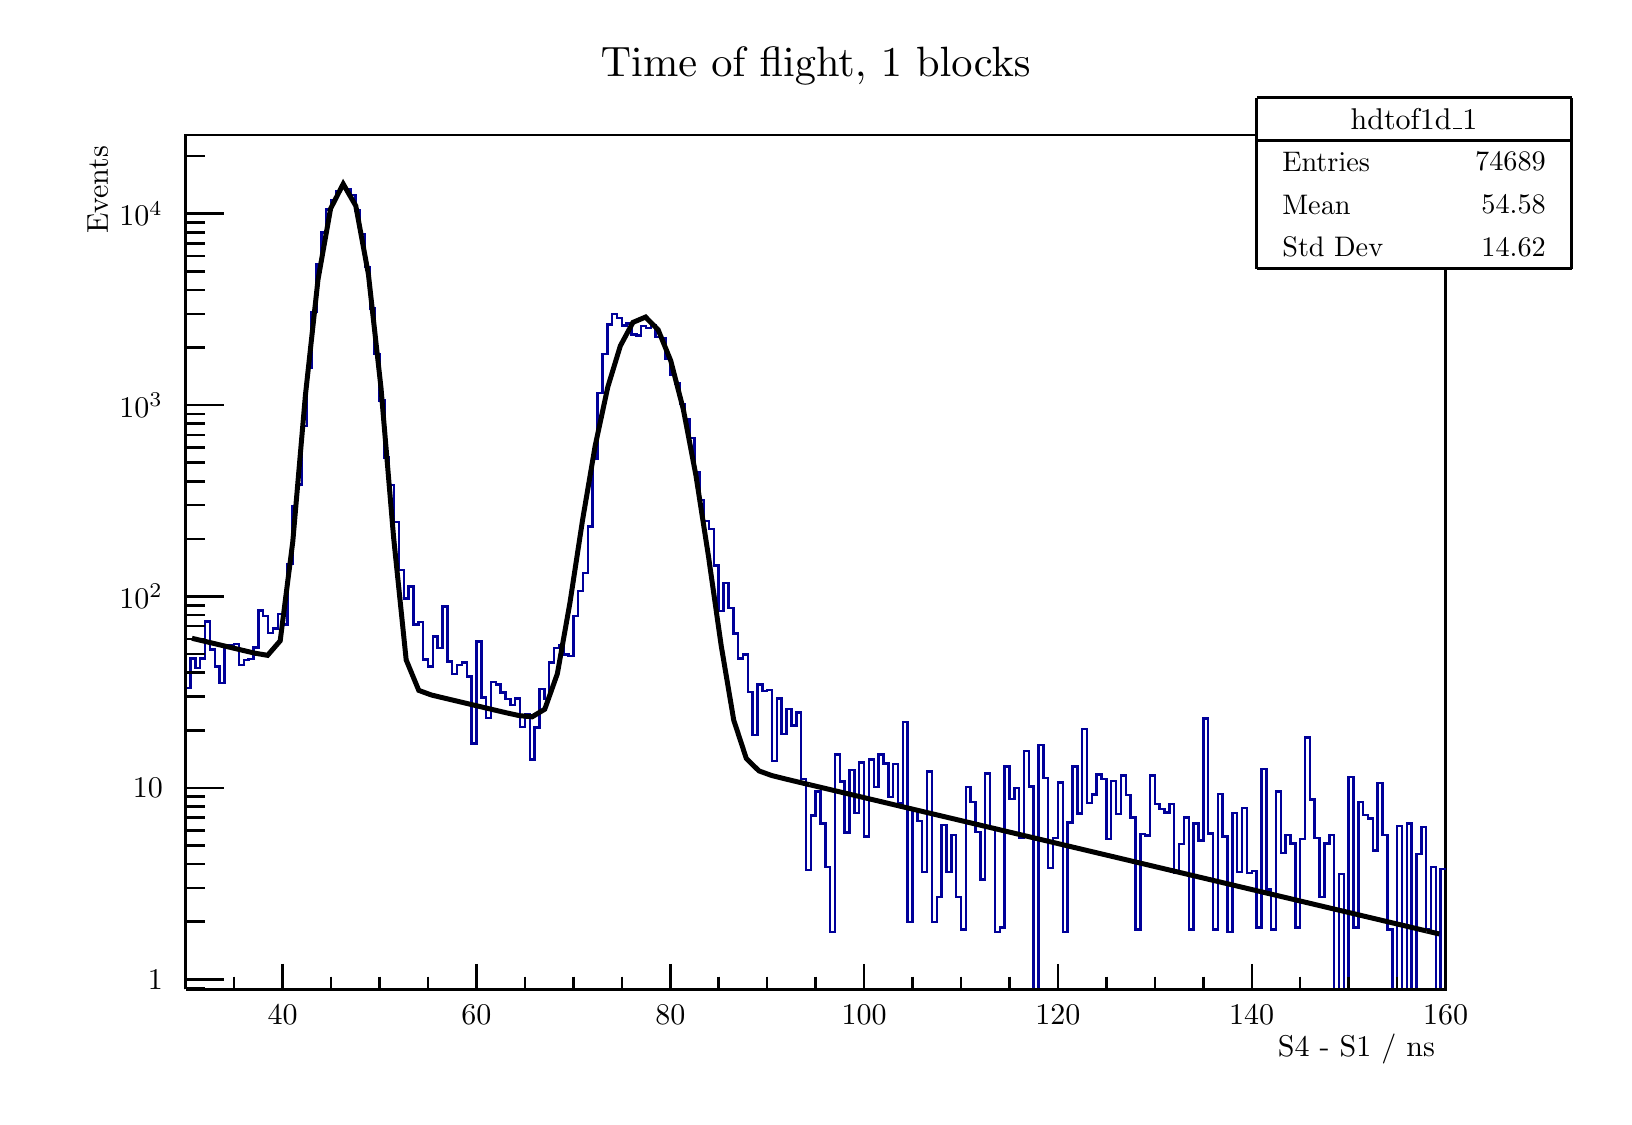
\begin{tikzpicture}
\pgfdeclareplotmark{cross} {
\pgfpathmoveto{\pgfpoint{-0.3\pgfplotmarksize}{\pgfplotmarksize}}
\pgfpathlineto{\pgfpoint{+0.3\pgfplotmarksize}{\pgfplotmarksize}}
\pgfpathlineto{\pgfpoint{+0.3\pgfplotmarksize}{0.3\pgfplotmarksize}}
\pgfpathlineto{\pgfpoint{+1\pgfplotmarksize}{0.3\pgfplotmarksize}}
\pgfpathlineto{\pgfpoint{+1\pgfplotmarksize}{-0.3\pgfplotmarksize}}
\pgfpathlineto{\pgfpoint{+0.3\pgfplotmarksize}{-0.3\pgfplotmarksize}}
\pgfpathlineto{\pgfpoint{+0.3\pgfplotmarksize}{-1.\pgfplotmarksize}}
\pgfpathlineto{\pgfpoint{-0.3\pgfplotmarksize}{-1.\pgfplotmarksize}}
\pgfpathlineto{\pgfpoint{-0.3\pgfplotmarksize}{-0.3\pgfplotmarksize}}
\pgfpathlineto{\pgfpoint{-1.\pgfplotmarksize}{-0.3\pgfplotmarksize}}
\pgfpathlineto{\pgfpoint{-1.\pgfplotmarksize}{0.3\pgfplotmarksize}}
\pgfpathlineto{\pgfpoint{-0.3\pgfplotmarksize}{0.3\pgfplotmarksize}}
\pgfpathclose
\pgfusepathqstroke
}
\pgfdeclareplotmark{cross*} {
\pgfpathmoveto{\pgfpoint{-0.3\pgfplotmarksize}{\pgfplotmarksize}}
\pgfpathlineto{\pgfpoint{+0.3\pgfplotmarksize}{\pgfplotmarksize}}
\pgfpathlineto{\pgfpoint{+0.3\pgfplotmarksize}{0.3\pgfplotmarksize}}
\pgfpathlineto{\pgfpoint{+1\pgfplotmarksize}{0.3\pgfplotmarksize}}
\pgfpathlineto{\pgfpoint{+1\pgfplotmarksize}{-0.3\pgfplotmarksize}}
\pgfpathlineto{\pgfpoint{+0.3\pgfplotmarksize}{-0.3\pgfplotmarksize}}
\pgfpathlineto{\pgfpoint{+0.3\pgfplotmarksize}{-1.\pgfplotmarksize}}
\pgfpathlineto{\pgfpoint{-0.3\pgfplotmarksize}{-1.\pgfplotmarksize}}
\pgfpathlineto{\pgfpoint{-0.3\pgfplotmarksize}{-0.3\pgfplotmarksize}}
\pgfpathlineto{\pgfpoint{-1.\pgfplotmarksize}{-0.3\pgfplotmarksize}}
\pgfpathlineto{\pgfpoint{-1.\pgfplotmarksize}{0.3\pgfplotmarksize}}
\pgfpathlineto{\pgfpoint{-0.3\pgfplotmarksize}{0.3\pgfplotmarksize}}
\pgfpathclose
\pgfusepathqfillstroke
}
\pgfdeclareplotmark{newstar} {
\pgfpathmoveto{\pgfqpoint{0pt}{\pgfplotmarksize}}
\pgfpathlineto{\pgfqpointpolar{44}{0.5\pgfplotmarksize}}
\pgfpathlineto{\pgfqpointpolar{18}{\pgfplotmarksize}}
\pgfpathlineto{\pgfqpointpolar{-20}{0.5\pgfplotmarksize}}
\pgfpathlineto{\pgfqpointpolar{-54}{\pgfplotmarksize}}
\pgfpathlineto{\pgfqpointpolar{-90}{0.5\pgfplotmarksize}}
\pgfpathlineto{\pgfqpointpolar{234}{\pgfplotmarksize}}
\pgfpathlineto{\pgfqpointpolar{198}{0.5\pgfplotmarksize}}
\pgfpathlineto{\pgfqpointpolar{162}{\pgfplotmarksize}}
\pgfpathlineto{\pgfqpointpolar{134}{0.5\pgfplotmarksize}}
\pgfpathclose
\pgfusepathqstroke
}
\pgfdeclareplotmark{newstar*} {
\pgfpathmoveto{\pgfqpoint{0pt}{\pgfplotmarksize}}
\pgfpathlineto{\pgfqpointpolar{44}{0.5\pgfplotmarksize}}
\pgfpathlineto{\pgfqpointpolar{18}{\pgfplotmarksize}}
\pgfpathlineto{\pgfqpointpolar{-20}{0.5\pgfplotmarksize}}
\pgfpathlineto{\pgfqpointpolar{-54}{\pgfplotmarksize}}
\pgfpathlineto{\pgfqpointpolar{-90}{0.5\pgfplotmarksize}}
\pgfpathlineto{\pgfqpointpolar{234}{\pgfplotmarksize}}
\pgfpathlineto{\pgfqpointpolar{198}{0.5\pgfplotmarksize}}
\pgfpathlineto{\pgfqpointpolar{162}{\pgfplotmarksize}}
\pgfpathlineto{\pgfqpointpolar{134}{0.5\pgfplotmarksize}}
\pgfpathclose
\pgfusepathqfillstroke
}
\definecolor{c}{rgb}{1,1,1};
\draw [color=c, fill=c] (0,0) rectangle (20,13.5632);
\draw [color=c, fill=c] (2,1.35632) rectangle (18,12.2069);
\definecolor{c}{rgb}{0,0,0};
\draw [c,line width=0.9] (2,1.35632) -- (2,12.2069) -- (18,12.2069) -- (18,1.35632) -- (2,1.35632);
\definecolor{c}{rgb}{1,1,1};
\draw [color=c, fill=c] (2,1.35632) rectangle (18,12.2069);
\definecolor{c}{rgb}{0,0,0};
\draw [c,line width=0.9] (2,1.35632) -- (2,12.2069) -- (18,12.2069) -- (18,1.35632) -- (2,1.35632);
\definecolor{c}{rgb}{0,0,0.6};
\draw [c,line width=0.9] (2,5.18151) -- (2.06154,5.18151) -- (2.06154,5.55608) -- (2.12308,5.55608) -- (2.12308,5.43961) -- (2.18462,5.43961) -- (2.18462,5.55581) -- (2.24615,5.55581) -- (2.24615,6.03099) -- (2.30769,6.03099) -- (2.30769,5.671) --
 (2.36923,5.671) -- (2.36923,5.45689) -- (2.43077,5.45689) -- (2.43077,5.24567) -- (2.49231,5.24567) -- (2.49231,5.73078) -- (2.55385,5.73078) -- (2.55385,5.72665) -- (2.61538,5.72665) -- (2.61538,5.74226) -- (2.67692,5.74226) -- (2.67692,5.47851) --
 (2.73846,5.47851) -- (2.73846,5.53808) -- (2.8,5.53808) -- (2.8,5.54976) -- (2.86154,5.54976) -- (2.86154,5.69856) -- (2.92308,5.69856) -- (2.92308,6.16999) -- (2.98462,6.16999) -- (2.98462,6.10032) -- (3.04615,6.10032) -- (3.04615,5.88449) --
 (3.10769,5.88449) -- (3.10769,5.93992) -- (3.16923,5.93992) -- (3.16923,6.12156) -- (3.23077,6.12156) -- (3.23077,5.99356) -- (3.29231,5.99356) -- (3.29231,6.75831) -- (3.35385,6.75831) -- (3.35385,7.49725) -- (3.41538,7.49725) -- (3.41538,7.76618)
 -- (3.47692,7.76618) -- (3.47692,8.5123) -- (3.53846,8.5123) -- (3.53846,9.25065) -- (3.6,9.25065) -- (3.6,9.95823) -- (3.66154,9.95823) -- (3.66154,10.5598) -- (3.72308,10.5598) -- (3.72308,10.9657) -- (3.78462,10.9657) -- (3.78462,11.2595) --
 (3.84615,11.2595) -- (3.84615,11.3826) -- (3.90769,11.3826) -- (3.90769,11.4937) -- (3.96923,11.4937) -- (3.96923,11.5322) -- (4.03077,11.5322) -- (4.03077,11.5125) -- (4.09231,11.5125) -- (4.09231,11.4476) -- (4.15385,11.4476) -- (4.15385,11.2503)
 -- (4.21538,11.2503) -- (4.21538,10.9505) -- (4.27692,10.9505) -- (4.27692,10.5305) -- (4.33846,10.5305) -- (4.33846,10.0019) -- (4.4,10.0019) -- (4.4,9.42602) -- (4.46154,9.42602) -- (4.46154,8.83371) -- (4.52308,8.83371) -- (4.52308,8.11005) --
 (4.58462,8.11005) -- (4.58462,7.76378) -- (4.64615,7.76378) -- (4.64615,7.29171) -- (4.70769,7.29171) -- (4.70769,6.67972) -- (4.76923,6.67972) -- (4.76923,6.32169) -- (4.83077,6.32169) -- (4.83077,6.47204) -- (4.89231,6.47204) -- (4.89231,5.993) --
 (4.95385,5.993) -- (4.95385,6.02017) -- (5.01538,6.02017) -- (5.01538,5.54748) -- (5.07692,5.54748) -- (5.07692,5.45714) -- (5.13846,5.45714) -- (5.13846,5.83864) -- (5.2,5.83864) -- (5.2,5.69096) -- (5.26154,5.69096) -- (5.26154,6.21606) --
 (5.32308,6.21606) -- (5.32308,5.51754) -- (5.38462,5.51754) -- (5.38462,5.35984) -- (5.44615,5.35984) -- (5.44615,5.47524) -- (5.50769,5.47524) -- (5.50769,5.50812) -- (5.56923,5.50812) -- (5.56923,5.32886) -- (5.63077,5.32886) -- (5.63077,4.47719)
 -- (5.69231,4.47719) -- (5.69231,5.77627) -- (5.75385,5.77627) -- (5.75385,5.06195) -- (5.81538,5.06195) -- (5.81538,4.80233) -- (5.87692,4.80233) -- (5.87692,5.25956) -- (5.93846,5.25956) -- (5.93846,5.22936) -- (6,5.22936) -- (6,5.12667) --
 (6.06154,5.12667) -- (6.06154,5.04604) -- (6.12308,5.04604) -- (6.12308,4.96718) -- (6.18462,4.96718) -- (6.18462,5.05252) -- (6.24615,5.05252) -- (6.24615,4.68623) -- (6.30769,4.68623) -- (6.30769,4.85157) -- (6.36923,4.85157) -- (6.36923,4.2741)
 -- (6.43077,4.2741) -- (6.43077,4.68523) -- (6.49231,4.68523) -- (6.49231,5.16964) -- (6.55385,5.16964) -- (6.55385,5.0443) -- (6.61538,5.0443) -- (6.61538,5.50863) -- (6.67692,5.50863) -- (6.67692,5.68975) -- (6.73846,5.68975) -- (6.73846,5.72166)
 -- (6.8,5.72166) -- (6.8,5.60763) -- (6.86154,5.60763) -- (6.86154,5.58722) -- (6.92308,5.58722) -- (6.92308,6.09935) -- (6.98462,6.09935) -- (6.98462,6.41753) -- (7.04615,6.41753) -- (7.04615,6.64659) -- (7.10769,6.64659) -- (7.10769,7.2355) --
 (7.16923,7.2355) -- (7.16923,8.09892) -- (7.23077,8.09892) -- (7.23077,8.93136) -- (7.29231,8.93136) -- (7.29231,9.42351) -- (7.35385,9.42351) -- (7.35385,9.79794) -- (7.41538,9.79794) -- (7.41538,9.93183) -- (7.47692,9.93183) -- (7.47692,9.8799) --
 (7.53846,9.8799) -- (7.53846,9.78722) -- (7.6,9.78722) -- (7.6,9.81608) -- (7.66154,9.81608) -- (7.66154,9.67331) -- (7.72308,9.67331) -- (7.72308,9.65902) -- (7.78462,9.65902) -- (7.78462,9.77948) -- (7.84615,9.77948) -- (7.84615,9.75876) --
 (7.90769,9.75876) -- (7.90769,9.79026) -- (7.96923,9.79026) -- (7.96923,9.64053) -- (8.03077,9.64053) -- (8.03077,9.63187) -- (8.09231,9.63187) -- (8.09231,9.36831) -- (8.15385,9.36831) -- (8.15385,9.16368) -- (8.21538,9.16368) -- (8.21538,9.05403)
 -- (8.27692,9.05403) -- (8.27692,8.78876) -- (8.33846,8.78876) -- (8.33846,8.603) -- (8.4,8.603) -- (8.4,8.35968) -- (8.46154,8.35968) -- (8.46154,7.91883) -- (8.52308,7.91883) -- (8.52308,7.56846) -- (8.58462,7.56846) -- (8.58462,7.30407) --
 (8.64615,7.30407) -- (8.64615,7.20532) -- (8.70769,7.20532) -- (8.70769,6.74177) -- (8.76923,6.74177) -- (8.76923,6.16352) -- (8.83077,6.16352) -- (8.83077,6.51821) -- (8.89231,6.51821) -- (8.89231,6.20221) -- (8.95385,6.20221) -- (8.95385,5.87638)
 -- (9.01538,5.87638) -- (9.01538,5.55625) -- (9.07692,5.55625) -- (9.07692,5.61066) -- (9.13846,5.61066) -- (9.13846,5.13328) -- (9.2,5.13328) -- (9.2,4.58783) -- (9.26154,4.58783) -- (9.26154,5.23012) -- (9.32308,5.23012) -- (9.32308,5.146) --
 (9.38461,5.146) -- (9.38461,5.15776) -- (9.44615,5.15776) -- (9.44615,4.25767) -- (9.50769,4.25767) -- (9.50769,5.04774) -- (9.56923,5.04774) -- (9.56923,4.60175) -- (9.63077,4.60175) -- (9.63077,4.92009) -- (9.69231,4.92009) -- (9.69231,4.71042) --
 (9.75385,4.71042) -- (9.75385,4.87061) -- (9.81538,4.87061) -- (9.81538,4.02592) -- (9.87692,4.02592) -- (9.87692,2.87449) -- (9.93846,2.87449) -- (9.93846,3.56693) -- (10,3.56693) -- (10,3.87246) -- (10.0615,3.87246) -- (10.0615,3.4613) --
 (10.1231,3.4613) -- (10.1231,2.90853) -- (10.1846,2.90853) -- (10.1846,2.08809) -- (10.2462,2.08809) -- (10.2462,4.33668) -- (10.3077,4.33668) -- (10.3077,3.99697) -- (10.3692,3.99697) -- (10.3692,3.3477) -- (10.4308,3.3477) -- (10.4308,4.13973) --
 (10.4923,4.13973) -- (10.4923,3.59781) -- (10.5538,3.59781) -- (10.5538,4.23774) -- (10.6154,4.23774) -- (10.6154,3.29987) -- (10.6769,3.29987) -- (10.6769,4.27622) -- (10.7385,4.27622) -- (10.7385,3.92545) -- (10.8,3.92545) -- (10.8,4.34213) --
 (10.8615,4.34213) -- (10.8615,4.22691) -- (10.9231,4.22691) -- (10.9231,3.79686) -- (10.9846,3.79686) -- (10.9846,4.22057) -- (11.0462,4.22057) -- (11.0462,3.71905) -- (11.1077,3.71905) -- (11.1077,4.75094) -- (11.1692,4.75094) -- (11.1692,2.20974)
 -- (11.2308,2.20974) -- (11.2308,3.65017) -- (11.2923,3.65017) -- (11.2923,3.492) -- (11.3538,3.492) -- (11.3538,2.84753) -- (11.4154,2.84753) -- (11.4154,4.12337) -- (11.4769,4.12337) -- (11.4769,2.20974) -- (11.5385,2.20974) -- (11.5385,2.53059)
 -- (11.6,2.53059) -- (11.6,3.44296) -- (11.6615,3.44296) -- (11.6615,2.84753) -- (11.7231,2.84753) -- (11.7231,3.31942) -- (11.7846,3.31942) -- (11.7846,2.53059) -- (11.8462,2.53059) -- (11.8462,2.11846) -- (11.9077,2.11846) -- (11.9077,3.92545) --
 (11.9692,3.92545) -- (11.9692,3.73625) -- (12.0308,3.73625) -- (12.0308,3.35377) -- (12.0923,3.35377) -- (12.0923,2.74928) -- (12.1538,2.74928) -- (12.1538,4.09554) -- (12.2154,4.09554) -- (12.2154,3.41687) -- (12.2769,3.41687) -- (12.2769,2.08809)
 -- (12.3385,2.08809) -- (12.3385,2.14272) -- (12.4,2.14272) -- (12.4,4.18641) -- (12.4615,4.18641) -- (12.4615,3.77723) -- (12.5231,3.77723) -- (12.5231,3.91398) -- (12.5846,3.91398) -- (12.5846,3.27829) -- (12.6462,3.27829) -- (12.6462,4.38363) --
 (12.7077,4.38363) -- (12.7077,3.93124) -- (12.7692,3.93124) -- (12.7692,1.35632) -- (12.8308,1.35632) -- (12.8308,4.45728) -- (12.8923,4.45728) -- (12.8923,4.04146) -- (12.9538,4.04146) -- (12.9538,2.89686) -- (13.0154,2.89686) -- (13.0154,3.27649)
 -- (13.0769,3.27649) -- (13.0769,3.98168) -- (13.1385,3.98168) -- (13.1385,2.08809) -- (13.2,2.08809) -- (13.2,3.47404) -- (13.2615,3.47404) -- (13.2615,4.18641) -- (13.3231,4.18641) -- (13.3231,3.58812) -- (13.3846,3.58812) -- (13.3846,4.66074) --
 (13.4462,4.66074) -- (13.4462,3.72096) -- (13.5077,3.72096) -- (13.5077,3.83058) -- (13.5692,3.83058) -- (13.5692,4.08766) -- (13.6308,4.08766) -- (13.6308,4.03023) -- (13.6923,4.03023) -- (13.6923,3.26645) -- (13.7538,3.26645) -- (13.7538,4.00415)
 -- (13.8154,4.00415) -- (13.8154,3.58678) -- (13.8769,3.58678) -- (13.8769,4.07563) -- (13.9385,4.07563) -- (13.9385,3.82377) -- (14,3.82377) -- (14,3.53914) -- (14.0615,3.53914) -- (14.0615,2.11846) -- (14.1231,2.11846) -- (14.1231,3.33056) --
 (14.1846,3.33056) -- (14.1846,3.3096) -- (14.2462,3.3096) -- (14.2462,4.07579) -- (14.3077,4.07579) -- (14.3077,3.70785) -- (14.3692,3.70785) -- (14.3692,3.64917) -- (14.4308,3.64917) -- (14.4308,3.60516) -- (14.4923,3.60516) -- (14.4923,3.70785) --
 (14.5538,3.70785) -- (14.5538,2.83516) -- (14.6154,2.83516) -- (14.6154,3.20139) -- (14.6769,3.20139) -- (14.6769,3.53914) -- (14.7385,3.53914) -- (14.7385,2.11846) -- (14.8,2.11846) -- (14.8,3.46572) -- (14.8615,3.46572) -- (14.8615,3.24538) --
 (14.9231,3.24538) -- (14.9231,4.79484) -- (14.9846,4.79484) -- (14.9846,3.33729) -- (15.0462,3.33729) -- (15.0462,2.11846) -- (15.1077,2.11846) -- (15.1077,3.83614) -- (15.1692,3.83614) -- (15.1692,3.29647) -- (15.2308,3.29647) -- (15.2308,2.08809)
 -- (15.2923,2.08809) -- (15.2923,3.59713) -- (15.3538,3.59713) -- (15.3538,2.85023) -- (15.4154,2.85023) -- (15.4154,3.66286) -- (15.4769,3.66286) -- (15.4769,2.83516) -- (15.5385,2.83516) -- (15.5385,2.86243) -- (15.6,2.86243) -- (15.6,2.14272) --
 (15.6615,2.14272) -- (15.6615,4.15383) -- (15.7231,4.15383) -- (15.7231,2.62199) -- (15.7846,2.62199) -- (15.7846,2.11846) -- (15.8462,2.11846) -- (15.8462,3.87165) -- (15.9077,3.87165) -- (15.9077,3.08614) -- (15.9692,3.08614) -- (15.9692,3.31751)
 -- (16.0308,3.31751) -- (16.0308,3.21207) -- (16.0923,3.21207) -- (16.0923,2.14272) -- (16.1538,2.14272) -- (16.1538,3.26826) -- (16.2154,3.26826) -- (16.2154,4.55325) -- (16.2769,4.55325) -- (16.2769,3.77087) -- (16.3385,3.77087) --
 (16.3385,3.27829) -- (16.4,3.27829) -- (16.4,2.53059) -- (16.4615,2.53059) -- (16.4615,3.21207) -- (16.5231,3.21207) -- (16.5231,3.31751) -- (16.5846,3.31751) -- (16.5846,1.35632) -- (16.6462,1.35632) -- (16.6462,2.81986) -- (16.7077,2.81986) --
 (16.7077,1.35632) -- (16.7692,1.35632) -- (16.7692,4.05445) -- (16.8308,4.05445) -- (16.8308,2.14272) -- (16.8923,2.14272) -- (16.8923,3.7376) -- (16.9538,3.7376) -- (16.9538,3.57313) -- (17.0154,3.57313) -- (17.0154,3.52486) -- (17.0769,3.52486) --
 (17.0769,3.12021) -- (17.1385,3.12021) -- (17.1385,3.98035) -- (17.2,3.98035) -- (17.2,3.31751) -- (17.2615,3.31751) -- (17.2615,2.11846) -- (17.3231,2.11846) -- (17.3231,1.35632) -- (17.3846,1.35632) -- (17.3846,3.43423) -- (17.4462,3.43423) --
 (17.4462,1.35632) -- (17.5077,1.35632) -- (17.5077,3.4613) -- (17.5692,3.4613) -- (17.5692,1.35632) -- (17.6308,1.35632) -- (17.6308,3.07628) -- (17.6923,3.07628) -- (17.6923,3.41932) -- (17.7538,3.41932) -- (17.7538,2.11846) -- (17.8154,2.11846) --
 (17.8154,2.90853) -- (17.8769,2.90853) -- (17.8769,1.35632) -- (17.9385,1.35632) -- (17.9385,2.88244) -- (18,2.88244);
\definecolor{c}{rgb}{0,0,0};
\draw [c,line width=0.9] (2,1.35632) -- (18,1.35632);
\draw [anchor= east] (18,0.596782) node[scale=1.08496, color=c, rotate=0]{ S4 - S1 / ns};
\draw [c,line width=0.9] (3.23077,1.68184) -- (3.23077,1.35632);
\draw [c,line width=0.9] (3.84615,1.51908) -- (3.84615,1.35632);
\draw [c,line width=0.9] (4.46154,1.51908) -- (4.46154,1.35632);
\draw [c,line width=0.9] (5.07692,1.51908) -- (5.07692,1.35632);
\draw [c,line width=0.9] (5.69231,1.68184) -- (5.69231,1.35632);
\draw [c,line width=0.9] (6.30769,1.51908) -- (6.30769,1.35632);
\draw [c,line width=0.9] (6.92308,1.51908) -- (6.92308,1.35632);
\draw [c,line width=0.9] (7.53846,1.51908) -- (7.53846,1.35632);
\draw [c,line width=0.9] (8.15385,1.68184) -- (8.15385,1.35632);
\draw [c,line width=0.9] (8.76923,1.51908) -- (8.76923,1.35632);
\draw [c,line width=0.9] (9.38461,1.51908) -- (9.38461,1.35632);
\draw [c,line width=0.9] (10,1.51908) -- (10,1.35632);
\draw [c,line width=0.9] (10.6154,1.68184) -- (10.6154,1.35632);
\draw [c,line width=0.9] (11.2308,1.51908) -- (11.2308,1.35632);
\draw [c,line width=0.9] (11.8462,1.51908) -- (11.8462,1.35632);
\draw [c,line width=0.9] (12.4615,1.51908) -- (12.4615,1.35632);
\draw [c,line width=0.9] (13.0769,1.68184) -- (13.0769,1.35632);
\draw [c,line width=0.9] (13.6923,1.51908) -- (13.6923,1.35632);
\draw [c,line width=0.9] (14.3077,1.51908) -- (14.3077,1.35632);
\draw [c,line width=0.9] (14.9231,1.51908) -- (14.9231,1.35632);
\draw [c,line width=0.9] (15.5385,1.68184) -- (15.5385,1.35632);
\draw [c,line width=0.9] (16.1538,1.51908) -- (16.1538,1.35632);
\draw [c,line width=0.9] (16.7692,1.51908) -- (16.7692,1.35632);
\draw [c,line width=0.9] (17.3846,1.51908) -- (17.3846,1.35632);
\draw [c,line width=0.9] (18,1.68184) -- (18,1.35632);
\draw [c,line width=0.9] (3.23077,1.68184) -- (3.23077,1.35632);
\draw [c,line width=0.9] (2.61538,1.51908) -- (2.61538,1.35632);
\draw [c,line width=0.9] (2,1.51908) -- (2,1.35632);
\draw [anchor=base] (3.23077,0.908736) node[scale=1.08496, color=c, rotate=0]{40};
\draw [anchor=base] (5.69231,0.908736) node[scale=1.08496, color=c, rotate=0]{60};
\draw [anchor=base] (8.15385,0.908736) node[scale=1.08496, color=c, rotate=0]{80};
\draw [anchor=base] (10.6154,0.908736) node[scale=1.08496, color=c, rotate=0]{100};
\draw [anchor=base] (13.0769,0.908736) node[scale=1.08496, color=c, rotate=0]{120};
\draw [anchor=base] (15.5385,0.908736) node[scale=1.08496, color=c, rotate=0]{140};
\draw [anchor=base] (18,0.908736) node[scale=1.08496, color=c, rotate=0]{160};
\draw [c,line width=0.9] (2,1.35632) -- (2,12.2069);
\draw [anchor= east] (0.88,12.2069) node[scale=1.08496, color=c, rotate=90]{ Events};
\draw [c,line width=0.9] (2.24,1.37274) -- (2,1.37274);
\draw [c,line width=0.9] (2.48,1.48397) -- (2,1.48397);
\draw [anchor= east] (1.844,1.48397) node[scale=1.08496, color=c, rotate=0]{1};
\draw [c,line width=0.9] (2.24,2.21574) -- (2,2.21574);
\draw [c,line width=0.9] (2.24,2.6438) -- (2,2.6438);
\draw [c,line width=0.9] (2.24,2.94751) -- (2,2.94751);
\draw [c,line width=0.9] (2.24,3.18309) -- (2,3.18309);
\draw [c,line width=0.9] (2.24,3.37557) -- (2,3.37557);
\draw [c,line width=0.9] (2.24,3.53831) -- (2,3.53831);
\draw [c,line width=0.9] (2.24,3.67928) -- (2,3.67928);
\draw [c,line width=0.9] (2.24,3.80363) -- (2,3.80363);
\draw [c,line width=0.9] (2.48,3.91486) -- (2,3.91486);
\draw [anchor= east] (1.844,3.91486) node[scale=1.08496, color=c, rotate=0]{10};
\draw [c,line width=0.9] (2.24,4.64663) -- (2,4.64663);
\draw [c,line width=0.9] (2.24,5.07469) -- (2,5.07469);
\draw [c,line width=0.9] (2.24,5.3784) -- (2,5.3784);
\draw [c,line width=0.9] (2.24,5.61398) -- (2,5.61398);
\draw [c,line width=0.9] (2.24,5.80646) -- (2,5.80646);
\draw [c,line width=0.9] (2.24,5.9692) -- (2,5.9692);
\draw [c,line width=0.9] (2.24,6.11017) -- (2,6.11017);
\draw [c,line width=0.9] (2.24,6.23452) -- (2,6.23452);
\draw [c,line width=0.9] (2.48,6.34575) -- (2,6.34575);
\draw [anchor= east] (1.844,6.34575) node[scale=1.08496, color=c, rotate=0]{$10^{2}$};
\draw [c,line width=0.9] (2.24,7.07752) -- (2,7.07752);
\draw [c,line width=0.9] (2.24,7.50558) -- (2,7.50558);
\draw [c,line width=0.9] (2.24,7.80929) -- (2,7.80929);
\draw [c,line width=0.9] (2.24,8.04487) -- (2,8.04487);
\draw [c,line width=0.9] (2.24,8.23735) -- (2,8.23735);
\draw [c,line width=0.9] (2.24,8.40009) -- (2,8.40009);
\draw [c,line width=0.9] (2.24,8.54106) -- (2,8.54106);
\draw [c,line width=0.9] (2.24,8.66541) -- (2,8.66541);
\draw [c,line width=0.9] (2.48,8.77664) -- (2,8.77664);
\draw [anchor= east] (1.844,8.77664) node[scale=1.08496, color=c, rotate=0]{$10^{3}$};
\draw [c,line width=0.9] (2.24,9.50841) -- (2,9.50841);
\draw [c,line width=0.9] (2.24,9.93647) -- (2,9.93647);
\draw [c,line width=0.9] (2.24,10.2402) -- (2,10.2402);
\draw [c,line width=0.9] (2.24,10.4758) -- (2,10.4758);
\draw [c,line width=0.9] (2.24,10.6682) -- (2,10.6682);
\draw [c,line width=0.9] (2.24,10.831) -- (2,10.831);
\draw [c,line width=0.9] (2.24,10.9719) -- (2,10.9719);
\draw [c,line width=0.9] (2.24,11.0963) -- (2,11.0963);
\draw [c,line width=0.9] (2.48,11.2075) -- (2,11.2075);
\draw [anchor= east] (1.844,11.2075) node[scale=1.08496, color=c, rotate=0]{$10^{4}$};
\draw [c,line width=0.9] (2.24,11.9393) -- (2,11.9393);
\definecolor{c}{rgb}{1,1,1};
\draw [color=c, fill=c] (15.6,10.5115) rectangle (19.6,12.6816);
\definecolor{c}{rgb}{0,0,0};
\draw [c,line width=0.9] (15.6,10.5115) -- (19.6,10.5115);
\draw [c,line width=0.9] (19.6,10.5115) -- (19.6,12.6816);
\draw [c,line width=0.9] (19.6,12.6816) -- (15.6,12.6816);
\draw [c,line width=0.9] (15.6,12.6816) -- (15.6,10.5115);
\draw (17.6,12.4103) node[scale=1.08496, color=c, rotate=0]{hdtof1d\_1};
\draw [c,line width=0.9] (15.6,12.1391) -- (19.6,12.1391);
\draw [anchor= west] (15.8,11.8678) node[scale=1.02114, color=c, rotate=0]{Entries };
\draw [anchor= east] (19.4,11.8678) node[scale=1.02114, color=c, rotate=0]{ 74689};
\draw [anchor= west] (15.8,11.3253) node[scale=1.02114, color=c, rotate=0]{Mean  };
\draw [anchor= east] (19.4,11.3253) node[scale=1.02114, color=c, rotate=0]{  54.58};
\draw [anchor= west] (15.8,10.7828) node[scale=1.02114, color=c, rotate=0]{Std Dev   };
\draw [anchor= east] (19.4,10.7828) node[scale=1.02114, color=c, rotate=0]{  14.62};
\draw [c,line width=1.8] (2.08,5.81522) -- (2.24,5.77729) -- (2.4,5.73936) -- (2.56,5.70143) -- (2.72,5.6635) -- (2.88,5.62584) -- (3.04,5.59883) -- (3.2,5.783) -- (3.36,7.04462) -- (3.52,8.89992) -- (3.68,10.3694) -- (3.84,11.2716) -- (4,11.5852) --
 (4.16,11.3072) -- (4.32,10.4394) -- (4.48,8.9965) -- (4.64,7.0994) -- (4.8,5.54055) -- (4.96,5.1535) -- (5.12,5.09513) -- (5.28,5.05662) -- (5.44,5.01869) -- (5.6,4.98076) -- (5.76,4.94283) -- (5.92,4.90492) -- (6.08,4.86731) -- (6.24,4.83246) --
 (6.4,4.81808) -- (6.56,4.91497) -- (6.72,5.3653) -- (6.88,6.26787) -- (7.04,7.31709) -- (7.2,8.25867) -- (7.36,9.00435) -- (7.52,9.52953) -- (7.68,9.82711) -- (7.84,9.89492) -- (8,9.73249) -- (8.16,9.34039) -- (8.32,8.721) -- (8.48,7.88215) --
 (8.64,6.85117) -- (8.8,5.72561) -- (8.96,4.77556) -- (9.12,4.2879) -- (9.28,4.13137) -- (9.44,4.0733) -- (9.6,4.03279) -- (9.76,3.9946) -- (9.92,3.95665);
\draw [c,line width=1.8] (9.92,3.95665) -- (10.08,3.91871) -- (10.24,3.88078) -- (10.4,3.84285) -- (10.56,3.80492) -- (10.72,3.76699) -- (10.88,3.72906) -- (11.04,3.69113) -- (11.2,3.6532) -- (11.36,3.61527) -- (11.52,3.57734) -- (11.68,3.53941) --
 (11.84,3.50148) -- (12,3.46355) -- (12.16,3.42562) -- (12.32,3.38769) -- (12.48,3.34976) -- (12.64,3.31183) -- (12.8,3.2739) -- (12.96,3.23597) -- (13.12,3.19804) -- (13.28,3.16011) -- (13.44,3.12218) -- (13.6,3.08425) -- (13.76,3.04632) --
 (13.92,3.00839) -- (14.08,2.97046) -- (14.24,2.93253) -- (14.4,2.8946) -- (14.56,2.85667) -- (14.72,2.81874) -- (14.88,2.78081) -- (15.04,2.74288) -- (15.2,2.70495) -- (15.36,2.66702) -- (15.52,2.62909) -- (15.68,2.59116) -- (15.84,2.55323) --
 (16,2.5153) -- (16.16,2.47737) -- (16.32,2.43944) -- (16.48,2.40151) -- (16.64,2.36358) -- (16.8,2.32565) -- (16.96,2.28772) -- (17.12,2.24979) -- (17.28,2.21186) -- (17.44,2.17393) -- (17.6,2.136) -- (17.76,2.09807);
\draw [c,line width=1.8] (17.76,2.09807) -- (17.92,2.06014);
\draw (10,13.0816) node[scale=1.5317, color=c, rotate=0]{Time of flight, 1 blocks};
\end{tikzpicture}

		\end{adjustbox}
		\caption{Example of the time of flight spectrum observed in $S4$ with a combined signal and background function fitted (shown in black)}
		\label{fig:fitEx}
	\end{figure}

	To produce the data used in this analysis, an exponential background function is subtracted. 
	The parameters for this function are taken from the combined signal and background function.

	\begin{figure}[h]
		\begin{adjustbox}{max totalsize={.8\textwidth}{.5\textheight},center}
			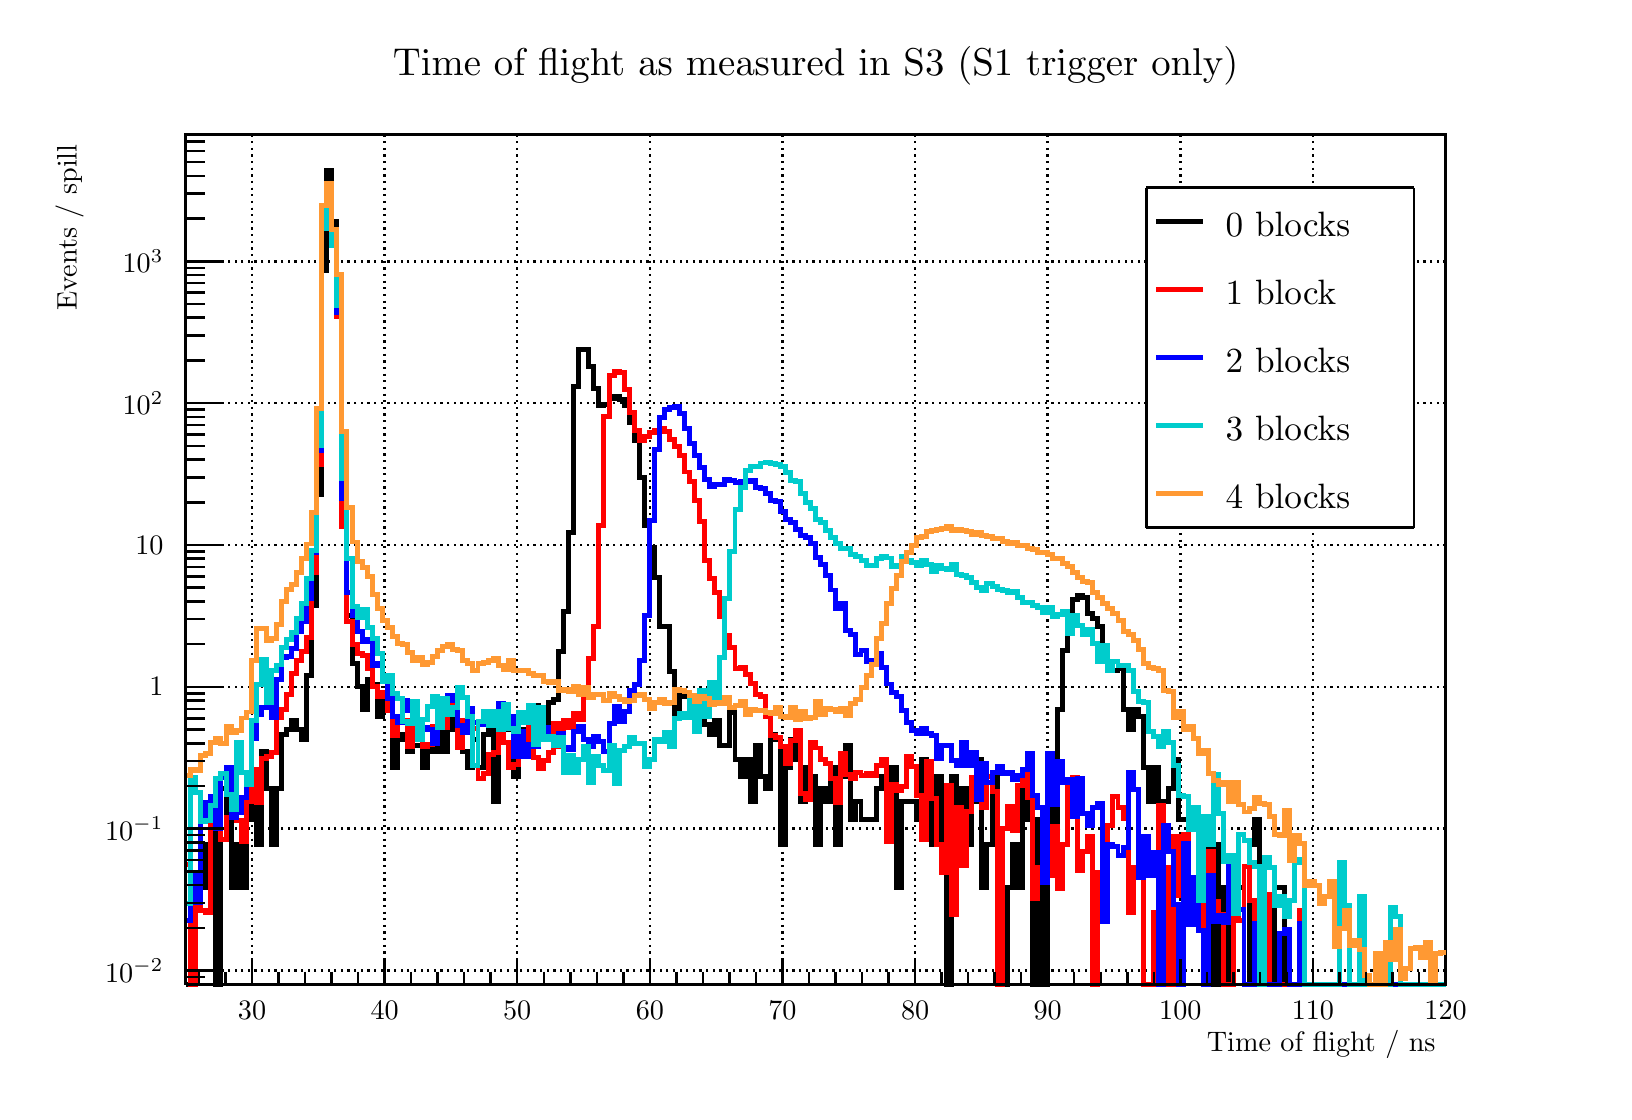
\begin{tikzpicture}
\pgfdeclareplotmark{cross} {
\pgfpathmoveto{\pgfpoint{-0.3\pgfplotmarksize}{\pgfplotmarksize}}
\pgfpathlineto{\pgfpoint{+0.3\pgfplotmarksize}{\pgfplotmarksize}}
\pgfpathlineto{\pgfpoint{+0.3\pgfplotmarksize}{0.3\pgfplotmarksize}}
\pgfpathlineto{\pgfpoint{+1\pgfplotmarksize}{0.3\pgfplotmarksize}}
\pgfpathlineto{\pgfpoint{+1\pgfplotmarksize}{-0.3\pgfplotmarksize}}
\pgfpathlineto{\pgfpoint{+0.3\pgfplotmarksize}{-0.3\pgfplotmarksize}}
\pgfpathlineto{\pgfpoint{+0.3\pgfplotmarksize}{-1.\pgfplotmarksize}}
\pgfpathlineto{\pgfpoint{-0.3\pgfplotmarksize}{-1.\pgfplotmarksize}}
\pgfpathlineto{\pgfpoint{-0.3\pgfplotmarksize}{-0.3\pgfplotmarksize}}
\pgfpathlineto{\pgfpoint{-1.\pgfplotmarksize}{-0.3\pgfplotmarksize}}
\pgfpathlineto{\pgfpoint{-1.\pgfplotmarksize}{0.3\pgfplotmarksize}}
\pgfpathlineto{\pgfpoint{-0.3\pgfplotmarksize}{0.3\pgfplotmarksize}}
\pgfpathclose
\pgfusepathqstroke
}
\pgfdeclareplotmark{cross*} {
\pgfpathmoveto{\pgfpoint{-0.3\pgfplotmarksize}{\pgfplotmarksize}}
\pgfpathlineto{\pgfpoint{+0.3\pgfplotmarksize}{\pgfplotmarksize}}
\pgfpathlineto{\pgfpoint{+0.3\pgfplotmarksize}{0.3\pgfplotmarksize}}
\pgfpathlineto{\pgfpoint{+1\pgfplotmarksize}{0.3\pgfplotmarksize}}
\pgfpathlineto{\pgfpoint{+1\pgfplotmarksize}{-0.3\pgfplotmarksize}}
\pgfpathlineto{\pgfpoint{+0.3\pgfplotmarksize}{-0.3\pgfplotmarksize}}
\pgfpathlineto{\pgfpoint{+0.3\pgfplotmarksize}{-1.\pgfplotmarksize}}
\pgfpathlineto{\pgfpoint{-0.3\pgfplotmarksize}{-1.\pgfplotmarksize}}
\pgfpathlineto{\pgfpoint{-0.3\pgfplotmarksize}{-0.3\pgfplotmarksize}}
\pgfpathlineto{\pgfpoint{-1.\pgfplotmarksize}{-0.3\pgfplotmarksize}}
\pgfpathlineto{\pgfpoint{-1.\pgfplotmarksize}{0.3\pgfplotmarksize}}
\pgfpathlineto{\pgfpoint{-0.3\pgfplotmarksize}{0.3\pgfplotmarksize}}
\pgfpathclose
\pgfusepathqfillstroke
}
\pgfdeclareplotmark{newstar} {
\pgfpathmoveto{\pgfqpoint{0pt}{\pgfplotmarksize}}
\pgfpathlineto{\pgfqpointpolar{44}{0.5\pgfplotmarksize}}
\pgfpathlineto{\pgfqpointpolar{18}{\pgfplotmarksize}}
\pgfpathlineto{\pgfqpointpolar{-20}{0.5\pgfplotmarksize}}
\pgfpathlineto{\pgfqpointpolar{-54}{\pgfplotmarksize}}
\pgfpathlineto{\pgfqpointpolar{-90}{0.5\pgfplotmarksize}}
\pgfpathlineto{\pgfqpointpolar{234}{\pgfplotmarksize}}
\pgfpathlineto{\pgfqpointpolar{198}{0.5\pgfplotmarksize}}
\pgfpathlineto{\pgfqpointpolar{162}{\pgfplotmarksize}}
\pgfpathlineto{\pgfqpointpolar{134}{0.5\pgfplotmarksize}}
\pgfpathclose
\pgfusepathqstroke
}
\pgfdeclareplotmark{newstar*} {
\pgfpathmoveto{\pgfqpoint{0pt}{\pgfplotmarksize}}
\pgfpathlineto{\pgfqpointpolar{44}{0.5\pgfplotmarksize}}
\pgfpathlineto{\pgfqpointpolar{18}{\pgfplotmarksize}}
\pgfpathlineto{\pgfqpointpolar{-20}{0.5\pgfplotmarksize}}
\pgfpathlineto{\pgfqpointpolar{-54}{\pgfplotmarksize}}
\pgfpathlineto{\pgfqpointpolar{-90}{0.5\pgfplotmarksize}}
\pgfpathlineto{\pgfqpointpolar{234}{\pgfplotmarksize}}
\pgfpathlineto{\pgfqpointpolar{198}{0.5\pgfplotmarksize}}
\pgfpathlineto{\pgfqpointpolar{162}{\pgfplotmarksize}}
\pgfpathlineto{\pgfqpointpolar{134}{0.5\pgfplotmarksize}}
\pgfpathclose
\pgfusepathqfillstroke
}
\definecolor{c}{rgb}{1,1,1};
\draw [color=c, fill=c] (0,0) rectangle (20,13.4957);
\draw [color=c, fill=c] (2,1.34957) rectangle (18,12.1461);
\definecolor{c}{rgb}{0,0,0};
\draw [c,line width=0.9] (2,1.34957) -- (2,12.1461) -- (18,12.1461) -- (18,1.34957) -- (2,1.34957);
\definecolor{c}{rgb}{1,1,1};
\draw [color=c, fill=c] (2,1.34957) rectangle (18,12.1461);
\definecolor{c}{rgb}{0,0,0};
\draw [c,line width=0.9] (2,1.34957) -- (2,12.1461) -- (18,12.1461) -- (18,1.34957) -- (2,1.34957);
\draw [c,line width=0.9] (2,1.34957) -- (18,1.34957);
\draw [c,dash pattern=on 0.80pt off 1.60pt ,line width=0.9] (2.84211,12.1461) -- (2.84211,1.34957);
\draw [c,dash pattern=on 0.80pt off 1.60pt ,line width=0.9] (4.52632,12.1461) -- (4.52632,1.34957);
\draw [c,dash pattern=on 0.80pt off 1.60pt ,line width=0.9] (6.21053,12.1461) -- (6.21053,1.34957);
\draw [c,dash pattern=on 0.80pt off 1.60pt ,line width=0.9] (7.89474,12.1461) -- (7.89474,1.34957);
\draw [c,dash pattern=on 0.80pt off 1.60pt ,line width=0.9] (9.57895,12.1461) -- (9.57895,1.34957);
\draw [c,dash pattern=on 0.80pt off 1.60pt ,line width=0.9] (11.2632,12.1461) -- (11.2632,1.34957);
\draw [c,dash pattern=on 0.80pt off 1.60pt ,line width=0.9] (12.9474,12.1461) -- (12.9474,1.34957);
\draw [c,dash pattern=on 0.80pt off 1.60pt ,line width=0.9] (14.6316,12.1461) -- (14.6316,1.34957);
\draw [c,dash pattern=on 0.80pt off 1.60pt ,line width=0.9] (16.3158,12.1461) -- (16.3158,1.34957);
\draw [c,dash pattern=on 0.80pt off 1.60pt ,line width=0.9] (18,12.1461) -- (18,1.34957);
\draw [c,dash pattern=on 0.80pt off 1.60pt ,line width=0.9] (2.84211,12.1461) -- (2.84211,1.34957);
\draw [c,line width=0.9] (2,1.34957) -- (2,12.1461);
\draw [c,dash pattern=on 0.80pt off 1.60pt ,line width=0.9] (18,1.52828) -- (2,1.52828);
\draw [c,dash pattern=on 0.80pt off 1.60pt ,line width=0.9] (18,3.32984) -- (2,3.32984);
\draw [c,dash pattern=on 0.80pt off 1.60pt ,line width=0.9] (18,5.1314) -- (2,5.1314);
\draw [c,dash pattern=on 0.80pt off 1.60pt ,line width=0.9] (18,6.93296) -- (2,6.93296);
\draw [c,dash pattern=on 0.80pt off 1.60pt ,line width=0.9] (18,8.73452) -- (2,8.73452);
\draw [c,dash pattern=on 0.80pt off 1.60pt ,line width=0.9] (18,10.5361) -- (2,10.5361);
\definecolor{c}{rgb}{0,0,0.6};
\draw [c,line width=0.9] (2,1.34957) -- (2.064,1.34957) -- (2.064,1.34957) -- (2.128,1.34957) -- (2.128,1.34957) -- (2.192,1.34957) -- (2.192,1.34957) -- (2.256,1.34957) -- (2.256,1.34957) -- (2.32,1.34957) -- (2.32,1.34957) -- (2.384,1.34957) --
 (2.384,1.34957) -- (2.448,1.34957) -- (2.448,1.34957) -- (2.512,1.34957) -- (2.512,1.34957) -- (2.576,1.34957) -- (2.576,1.34957) -- (2.64,1.34957) -- (2.64,1.34957) -- (2.704,1.34957) -- (2.704,1.34957) -- (2.768,1.34957) -- (2.768,1.34957) --
 (2.832,1.34957) -- (2.832,1.34957) -- (2.896,1.34957) -- (2.896,1.34957) -- (2.96,1.34957) -- (2.96,1.34957) -- (3.024,1.34957) -- (3.024,1.34957) -- (3.088,1.34957) -- (3.088,1.34957) -- (3.152,1.34957) -- (3.152,1.34957) -- (3.216,1.34957) --
 (3.216,1.34957) -- (3.28,1.34957) -- (3.28,1.34957) -- (3.344,1.34957) -- (3.344,1.34957) -- (3.408,1.34957) -- (3.408,1.34957) -- (3.472,1.34957) -- (3.472,1.34957) -- (3.536,1.34957) -- (3.536,1.34957) -- (3.6,1.34957) -- (3.6,1.34957) --
 (3.664,1.34957) -- (3.664,1.34957) -- (3.728,1.34957) -- (3.728,1.34957) -- (3.792,1.34957) -- (3.792,1.34957) -- (3.856,1.34957) -- (3.856,1.34957) -- (3.92,1.34957) -- (3.92,1.34957) -- (3.984,1.34957) -- (3.984,1.34957) -- (4.048,1.34957) --
 (4.048,1.34957) -- (4.112,1.34957) -- (4.112,1.34957) -- (4.176,1.34957) -- (4.176,1.34957) -- (4.24,1.34957) -- (4.24,1.34957) -- (4.304,1.34957) -- (4.304,1.34957) -- (4.368,1.34957) -- (4.368,1.34957) -- (4.432,1.34957) -- (4.432,1.34957) --
 (4.496,1.34957) -- (4.496,1.34957) -- (4.56,1.34957) -- (4.56,1.34957) -- (4.624,1.34957) -- (4.624,1.34957) -- (4.688,1.34957) -- (4.688,1.34957) -- (4.752,1.34957) -- (4.752,1.34957) -- (4.816,1.34957) -- (4.816,1.34957) -- (4.88,1.34957) --
 (4.88,1.34957) -- (4.944,1.34957) -- (4.944,1.34957) -- (5.008,1.34957) -- (5.008,1.34957) -- (5.072,1.34957) -- (5.072,1.34957) -- (5.136,1.34957) -- (5.136,1.34957) -- (5.2,1.34957) -- (5.2,1.34957) -- (5.264,1.34957) -- (5.264,1.34957) --
 (5.328,1.34957) -- (5.328,1.34957) -- (5.392,1.34957) -- (5.392,1.34957) -- (5.456,1.34957) -- (5.456,1.34957) -- (5.52,1.34957) -- (5.52,1.34957) -- (5.584,1.34957) -- (5.584,1.34957) -- (5.648,1.34957) -- (5.648,1.34957) -- (5.712,1.34957) --
 (5.712,1.34957) -- (5.776,1.34957) -- (5.776,1.34957) -- (5.84,1.34957) -- (5.84,1.34957) -- (5.904,1.34957) -- (5.904,1.34957) -- (5.968,1.34957) -- (5.968,1.34957) -- (6.032,1.34957) -- (6.032,1.34957) -- (6.096,1.34957) -- (6.096,1.34957) --
 (6.16,1.34957) -- (6.16,1.34957) -- (6.224,1.34957) -- (6.224,1.34957) -- (6.288,1.34957) -- (6.288,1.34957) -- (6.352,1.34957) -- (6.352,1.34957) -- (6.416,1.34957) -- (6.416,1.34957) -- (6.48,1.34957) -- (6.48,1.34957) -- (6.544,1.34957) --
 (6.544,1.34957) -- (6.608,1.34957) -- (6.608,1.34957) -- (6.672,1.34957) -- (6.672,1.34957) -- (6.736,1.34957) -- (6.736,1.34957) -- (6.8,1.34957) -- (6.8,1.34957) -- (6.864,1.34957) -- (6.864,1.34957) -- (6.928,1.34957) -- (6.928,1.34957) --
 (6.992,1.34957) -- (6.992,1.34957) -- (7.056,1.34957) -- (7.056,1.34957) -- (7.12,1.34957) -- (7.12,1.34957) -- (7.184,1.34957) -- (7.184,1.34957) -- (7.248,1.34957) -- (7.248,1.34957) -- (7.312,1.34957) -- (7.312,1.34957) -- (7.376,1.34957) --
 (7.376,1.34957) -- (7.44,1.34957) -- (7.44,1.34957) -- (7.504,1.34957) -- (7.504,1.34957) -- (7.568,1.34957) -- (7.568,1.34957) -- (7.632,1.34957) -- (7.632,1.34957) -- (7.696,1.34957) -- (7.696,1.34957) -- (7.76,1.34957) -- (7.76,1.34957) --
 (7.824,1.34957) -- (7.824,1.34957) -- (7.888,1.34957) -- (7.888,1.34957) -- (7.952,1.34957) -- (7.952,1.34957) -- (8.016,1.34957) -- (8.016,1.34957) -- (8.08,1.34957) -- (8.08,1.34957) -- (8.144,1.34957) -- (8.144,1.34957) -- (8.208,1.34957) --
 (8.208,1.34957) -- (8.272,1.34957) -- (8.272,1.34957) -- (8.336,1.34957) -- (8.336,1.34957) -- (8.4,1.34957) -- (8.4,1.34957) -- (8.464,1.34957) -- (8.464,1.34957) -- (8.528,1.34957) -- (8.528,1.34957) -- (8.592,1.34957) -- (8.592,1.34957) --
 (8.656,1.34957) -- (8.656,1.34957) -- (8.72,1.34957) -- (8.72,1.34957) -- (8.784,1.34957) -- (8.784,1.34957) -- (8.848,1.34957) -- (8.848,1.34957) -- (8.912,1.34957) -- (8.912,1.34957) -- (8.976,1.34957) -- (8.976,1.34957) -- (9.04,1.34957) --
 (9.04,1.34957) -- (9.104,1.34957) -- (9.104,1.34957) -- (9.168,1.34957) -- (9.168,1.34957) -- (9.232,1.34957) -- (9.232,1.34957) -- (9.296,1.34957) -- (9.296,1.34957) -- (9.36,1.34957) -- (9.36,1.34957) -- (9.424,1.34957) -- (9.424,1.34957) --
 (9.488,1.34957) -- (9.488,1.34957) -- (9.552,1.34957) -- (9.552,1.34957) -- (9.616,1.34957) -- (9.616,1.34957) -- (9.68,1.34957) -- (9.68,1.34957) -- (9.744,1.34957) -- (9.744,1.34957) -- (9.808,1.34957) -- (9.808,1.34957) -- (9.872,1.34957) --
 (9.872,1.34957) -- (9.936,1.34957) -- (9.936,1.34957) -- (10,1.34957) -- (10,1.34957) -- (10.064,1.34957) -- (10.064,1.34957) -- (10.128,1.34957) -- (10.128,1.34957) -- (10.192,1.34957) -- (10.192,1.34957) -- (10.256,1.34957) -- (10.256,1.34957) --
 (10.32,1.34957) -- (10.32,1.34957) -- (10.384,1.34957) -- (10.384,1.34957) -- (10.448,1.34957) -- (10.448,1.34957) -- (10.512,1.34957) -- (10.512,1.34957) -- (10.576,1.34957) -- (10.576,1.34957) -- (10.64,1.34957) -- (10.64,1.34957) --
 (10.704,1.34957) -- (10.704,1.34957) -- (10.768,1.34957) -- (10.768,1.34957) -- (10.832,1.34957) -- (10.832,1.34957) -- (10.896,1.34957) -- (10.896,1.34957) -- (10.96,1.34957) -- (10.96,1.34957) -- (11.024,1.34957) -- (11.024,1.34957) --
 (11.088,1.34957) -- (11.088,1.34957) -- (11.152,1.34957) -- (11.152,1.34957) -- (11.216,1.34957) -- (11.216,1.34957) -- (11.28,1.34957) -- (11.28,1.34957) -- (11.344,1.34957) -- (11.344,1.34957) -- (11.408,1.34957) -- (11.408,1.34957) --
 (11.472,1.34957) -- (11.472,1.34957) -- (11.536,1.34957) -- (11.536,1.34957) -- (11.6,1.34957) -- (11.6,1.34957) -- (11.664,1.34957) -- (11.664,1.34957) -- (11.728,1.34957) -- (11.728,1.34957) -- (11.792,1.34957) -- (11.792,1.34957) --
 (11.856,1.34957) -- (11.856,1.34957) -- (11.92,1.34957) -- (11.92,1.34957) -- (11.984,1.34957) -- (11.984,1.34957) -- (12.048,1.34957) -- (12.048,1.34957) -- (12.112,1.34957) -- (12.112,1.34957) -- (12.176,1.34957) -- (12.176,1.34957) --
 (12.24,1.34957) -- (12.24,1.34957) -- (12.304,1.34957) -- (12.304,1.34957) -- (12.368,1.34957) -- (12.368,1.34957) -- (12.432,1.34957) -- (12.432,1.34957) -- (12.496,1.34957) -- (12.496,1.34957) -- (12.56,1.34957) -- (12.56,1.34957) --
 (12.624,1.34957) -- (12.624,1.34957) -- (12.688,1.34957) -- (12.688,1.34957) -- (12.752,1.34957) -- (12.752,1.34957) -- (12.816,1.34957) -- (12.816,1.34957) -- (12.88,1.34957) -- (12.88,1.34957) -- (12.944,1.34957) -- (12.944,1.34957) --
 (13.008,1.34957) -- (13.008,1.34957) -- (13.072,1.34957) -- (13.072,1.34957) -- (13.136,1.34957) -- (13.136,1.34957) -- (13.2,1.34957) -- (13.2,1.34957) -- (13.264,1.34957) -- (13.264,1.34957) -- (13.328,1.34957) -- (13.328,1.34957) --
 (13.392,1.34957) -- (13.392,1.34957) -- (13.456,1.34957) -- (13.456,1.34957) -- (13.52,1.34957) -- (13.52,1.34957) -- (13.584,1.34957) -- (13.584,1.34957) -- (13.648,1.34957) -- (13.648,1.34957) -- (13.712,1.34957) -- (13.712,1.34957) --
 (13.776,1.34957) -- (13.776,1.34957) -- (13.84,1.34957) -- (13.84,1.34957) -- (13.904,1.34957) -- (13.904,1.34957) -- (13.968,1.34957) -- (13.968,1.34957) -- (14.032,1.34957) -- (14.032,1.34957) -- (14.096,1.34957) -- (14.096,1.34957) --
 (14.16,1.34957) -- (14.16,1.34957) -- (14.224,1.34957) -- (14.224,1.34957) -- (14.288,1.34957) -- (14.288,1.34957) -- (14.352,1.34957) -- (14.352,1.34957) -- (14.416,1.34957) -- (14.416,1.34957) -- (14.48,1.34957) -- (14.48,1.34957) --
 (14.544,1.34957) -- (14.544,1.34957) -- (14.608,1.34957) -- (14.608,1.34957) -- (14.672,1.34957) -- (14.672,1.34957) -- (14.736,1.34957) -- (14.736,1.34957) -- (14.8,1.34957) -- (14.8,1.34957) -- (14.864,1.34957) -- (14.864,1.34957) --
 (14.928,1.34957) -- (14.928,1.34957) -- (14.992,1.34957) -- (14.992,1.34957) -- (15.056,1.34957) -- (15.056,1.34957) -- (15.12,1.34957) -- (15.12,1.34957) -- (15.184,1.34957) -- (15.184,1.34957) -- (15.248,1.34957) -- (15.248,1.34957) --
 (15.312,1.34957) -- (15.312,1.34957) -- (15.376,1.34957) -- (15.376,1.34957) -- (15.44,1.34957) -- (15.44,1.34957) -- (15.504,1.34957) -- (15.504,1.34957) -- (15.568,1.34957) -- (15.568,1.34957) -- (15.632,1.34957) -- (15.632,1.34957) --
 (15.696,1.34957) -- (15.696,1.34957) -- (15.76,1.34957) -- (15.76,1.34957) -- (15.824,1.34957) -- (15.824,1.34957) -- (15.888,1.34957) -- (15.888,1.34957) -- (15.952,1.34957) -- (15.952,1.34957) -- (16.016,1.34957) -- (16.016,1.34957) --
 (16.08,1.34957) -- (16.08,1.34957) -- (16.144,1.34957) -- (16.144,1.34957) -- (16.208,1.34957) -- (16.208,1.34957) -- (16.272,1.34957) -- (16.272,1.34957) -- (16.336,1.34957) -- (16.336,1.34957) -- (16.4,1.34957) -- (16.4,1.34957) --
 (16.464,1.34957) -- (16.464,1.34957) -- (16.528,1.34957) -- (16.528,1.34957) -- (16.592,1.34957) -- (16.592,1.34957) -- (16.656,1.34957) -- (16.656,1.34957) -- (16.72,1.34957) -- (16.72,1.34957) -- (16.784,1.34957) -- (16.784,1.34957) --
 (16.848,1.34957) -- (16.848,1.34957) -- (16.912,1.34957) -- (16.912,1.34957) -- (16.976,1.34957) -- (16.976,1.34957) -- (17.04,1.34957) -- (17.04,1.34957) -- (17.104,1.34957) -- (17.104,1.34957) -- (17.168,1.34957) -- (17.168,1.34957) --
 (17.232,1.34957) -- (17.232,1.34957) -- (17.296,1.34957) -- (17.296,1.34957) -- (17.36,1.34957) -- (17.36,1.34957) -- (17.424,1.34957) -- (17.424,1.34957) -- (17.488,1.34957) -- (17.488,1.34957) -- (17.552,1.34957) -- (17.552,1.34957) --
 (17.616,1.34957) -- (17.616,1.34957) -- (17.68,1.34957) -- (17.68,1.34957) -- (17.744,1.34957) -- (17.744,1.34957) -- (17.808,1.34957) -- (17.808,1.34957) -- (17.872,1.34957) -- (17.872,1.34957) -- (17.936,1.34957) -- (17.936,1.34957) --
 (18,1.34957);
\definecolor{c}{rgb}{0,0,0};
\draw [c,line width=0.9] (2,1.34957) -- (18,1.34957);
\draw [c,line width=0.9] (2.84211,1.67347) -- (2.84211,1.34957);
\draw [c,line width=0.9] (3.17895,1.51152) -- (3.17895,1.34957);
\draw [c,line width=0.9] (3.51579,1.51152) -- (3.51579,1.34957);
\draw [c,line width=0.9] (3.85263,1.51152) -- (3.85263,1.34957);
\draw [c,line width=0.9] (4.18947,1.51152) -- (4.18947,1.34957);
\draw [c,line width=0.9] (4.52632,1.67347) -- (4.52632,1.34957);
\draw [c,line width=0.9] (4.86316,1.51152) -- (4.86316,1.34957);
\draw [c,line width=0.9] (5.2,1.51152) -- (5.2,1.34957);
\draw [c,line width=0.9] (5.53684,1.51152) -- (5.53684,1.34957);
\draw [c,line width=0.9] (5.87368,1.51152) -- (5.87368,1.34957);
\draw [c,line width=0.9] (6.21053,1.67347) -- (6.21053,1.34957);
\draw [c,line width=0.9] (6.54737,1.51152) -- (6.54737,1.34957);
\draw [c,line width=0.9] (6.88421,1.51152) -- (6.88421,1.34957);
\draw [c,line width=0.9] (7.22105,1.51152) -- (7.22105,1.34957);
\draw [c,line width=0.9] (7.55789,1.51152) -- (7.55789,1.34957);
\draw [c,line width=0.9] (7.89474,1.67347) -- (7.89474,1.34957);
\draw [c,line width=0.9] (8.23158,1.51152) -- (8.23158,1.34957);
\draw [c,line width=0.9] (8.56842,1.51152) -- (8.56842,1.34957);
\draw [c,line width=0.9] (8.90526,1.51152) -- (8.90526,1.34957);
\draw [c,line width=0.9] (9.24211,1.51152) -- (9.24211,1.34957);
\draw [c,line width=0.9] (9.57895,1.67347) -- (9.57895,1.34957);
\draw [c,line width=0.9] (9.91579,1.51152) -- (9.91579,1.34957);
\draw [c,line width=0.9] (10.2526,1.51152) -- (10.2526,1.34957);
\draw [c,line width=0.9] (10.5895,1.51152) -- (10.5895,1.34957);
\draw [c,line width=0.9] (10.9263,1.51152) -- (10.9263,1.34957);
\draw [c,line width=0.9] (11.2632,1.67347) -- (11.2632,1.34957);
\draw [c,line width=0.9] (11.6,1.51152) -- (11.6,1.34957);
\draw [c,line width=0.9] (11.9368,1.51152) -- (11.9368,1.34957);
\draw [c,line width=0.9] (12.2737,1.51152) -- (12.2737,1.34957);
\draw [c,line width=0.9] (12.6105,1.51152) -- (12.6105,1.34957);
\draw [c,line width=0.9] (12.9474,1.67347) -- (12.9474,1.34957);
\draw [c,line width=0.9] (13.2842,1.51152) -- (13.2842,1.34957);
\draw [c,line width=0.9] (13.6211,1.51152) -- (13.6211,1.34957);
\draw [c,line width=0.9] (13.9579,1.51152) -- (13.9579,1.34957);
\draw [c,line width=0.9] (14.2947,1.51152) -- (14.2947,1.34957);
\draw [c,line width=0.9] (14.6316,1.67347) -- (14.6316,1.34957);
\draw [c,line width=0.9] (14.9684,1.51152) -- (14.9684,1.34957);
\draw [c,line width=0.9] (15.3053,1.51152) -- (15.3053,1.34957);
\draw [c,line width=0.9] (15.6421,1.51152) -- (15.6421,1.34957);
\draw [c,line width=0.9] (15.9789,1.51152) -- (15.9789,1.34957);
\draw [c,line width=0.9] (16.3158,1.67347) -- (16.3158,1.34957);
\draw [c,line width=0.9] (16.6526,1.51152) -- (16.6526,1.34957);
\draw [c,line width=0.9] (16.9895,1.51152) -- (16.9895,1.34957);
\draw [c,line width=0.9] (17.3263,1.51152) -- (17.3263,1.34957);
\draw [c,line width=0.9] (17.6632,1.51152) -- (17.6632,1.34957);
\draw [c,line width=0.9] (18,1.67347) -- (18,1.34957);
\draw [c,line width=0.9] (2.84211,1.67347) -- (2.84211,1.34957);
\draw [c,line width=0.9] (2.50526,1.51152) -- (2.50526,1.34957);
\draw [c,line width=0.9] (2.16842,1.51152) -- (2.16842,1.34957);
\draw [anchor=base] (2.84211,0.904212) node[scale=1.01821, color=c, rotate=0]{30};
\draw [anchor=base] (4.52632,0.904212) node[scale=1.01821, color=c, rotate=0]{40};
\draw [anchor=base] (6.21053,0.904212) node[scale=1.01821, color=c, rotate=0]{50};
\draw [anchor=base] (7.89474,0.904212) node[scale=1.01821, color=c, rotate=0]{60};
\draw [anchor=base] (9.57895,0.904212) node[scale=1.01821, color=c, rotate=0]{70};
\draw [anchor=base] (11.2632,0.904212) node[scale=1.01821, color=c, rotate=0]{80};
\draw [anchor=base] (12.9474,0.904212) node[scale=1.01821, color=c, rotate=0]{90};
\draw [anchor=base] (14.6316,0.904212) node[scale=1.01821, color=c, rotate=0]{100};
\draw [anchor=base] (16.3158,0.904212) node[scale=1.01821, color=c, rotate=0]{110};
\draw [anchor=base] (18,0.904212) node[scale=1.01821, color=c, rotate=0]{120};
\draw [anchor= east] (18,0.593811) node[scale=1.01821, color=c, rotate=0]{ Time of flight / ns};
\draw [c,line width=0.9] (2,1.34957) -- (2,12.1461);
\draw [c,line width=0.9] (2.24,1.35369) -- (2,1.35369);
\draw [c,line width=0.9] (2.24,1.44585) -- (2,1.44585);
\draw [c,line width=0.9] (2.48,1.52828) -- (2,1.52828);
\draw [anchor= east] (1.844,1.52828) node[scale=1.01821, color=c, rotate=0]{$10^{-2}$};
\draw [c,line width=0.9] (2.24,2.07061) -- (2,2.07061);
\draw [c,line width=0.9] (2.24,2.38785) -- (2,2.38785);
\draw [c,line width=0.9] (2.24,2.61293) -- (2,2.61293);
\draw [c,line width=0.9] (2.24,2.78752) -- (2,2.78752);
\draw [c,line width=0.9] (2.24,2.93017) -- (2,2.93017);
\draw [c,line width=0.9] (2.24,3.05078) -- (2,3.05078);
\draw [c,line width=0.9] (2.24,3.15525) -- (2,3.15525);
\draw [c,line width=0.9] (2.24,3.24741) -- (2,3.24741);
\draw [c,line width=0.9] (2.48,3.32984) -- (2,3.32984);
\draw [anchor= east] (1.844,3.32984) node[scale=1.01821, color=c, rotate=0]{$10^{-1}$};
\draw [c,line width=0.9] (2.24,3.87217) -- (2,3.87217);
\draw [c,line width=0.9] (2.24,4.18941) -- (2,4.18941);
\draw [c,line width=0.9] (2.24,4.41449) -- (2,4.41449);
\draw [c,line width=0.9] (2.24,4.58908) -- (2,4.58908);
\draw [c,line width=0.9] (2.24,4.73173) -- (2,4.73173);
\draw [c,line width=0.9] (2.24,4.85234) -- (2,4.85234);
\draw [c,line width=0.9] (2.24,4.95681) -- (2,4.95681);
\draw [c,line width=0.9] (2.24,5.04897) -- (2,5.04897);
\draw [c,line width=0.9] (2.48,5.1314) -- (2,5.1314);
\draw [anchor= east] (1.844,5.1314) node[scale=1.01821, color=c, rotate=0]{1};
\draw [c,line width=0.9] (2.24,5.67373) -- (2,5.67373);
\draw [c,line width=0.9] (2.24,5.99096) -- (2,5.99096);
\draw [c,line width=0.9] (2.24,6.21605) -- (2,6.21605);
\draw [c,line width=0.9] (2.24,6.39064) -- (2,6.39064);
\draw [c,line width=0.9] (2.24,6.53329) -- (2,6.53329);
\draw [c,line width=0.9] (2.24,6.6539) -- (2,6.6539);
\draw [c,line width=0.9] (2.24,6.75837) -- (2,6.75837);
\draw [c,line width=0.9] (2.24,6.85053) -- (2,6.85053);
\draw [c,line width=0.9] (2.48,6.93296) -- (2,6.93296);
\draw [anchor= east] (1.844,6.93296) node[scale=1.01821, color=c, rotate=0]{10};
\draw [c,line width=0.9] (2.24,7.47529) -- (2,7.47529);
\draw [c,line width=0.9] (2.24,7.79252) -- (2,7.79252);
\draw [c,line width=0.9] (2.24,8.01761) -- (2,8.01761);
\draw [c,line width=0.9] (2.24,8.1922) -- (2,8.1922);
\draw [c,line width=0.9] (2.24,8.33485) -- (2,8.33485);
\draw [c,line width=0.9] (2.24,8.45546) -- (2,8.45546);
\draw [c,line width=0.9] (2.24,8.55993) -- (2,8.55993);
\draw [c,line width=0.9] (2.24,8.65209) -- (2,8.65209);
\draw [c,line width=0.9] (2.48,8.73452) -- (2,8.73452);
\draw [anchor= east] (1.844,8.73452) node[scale=1.01821, color=c, rotate=0]{$10^{2}$};
\draw [c,line width=0.9] (2.24,9.27684) -- (2,9.27684);
\draw [c,line width=0.9] (2.24,9.59408) -- (2,9.59408);
\draw [c,line width=0.9] (2.24,9.81917) -- (2,9.81917);
\draw [c,line width=0.9] (2.24,9.99376) -- (2,9.99376);
\draw [c,line width=0.9] (2.24,10.1364) -- (2,10.1364);
\draw [c,line width=0.9] (2.24,10.257) -- (2,10.257);
\draw [c,line width=0.9] (2.24,10.3615) -- (2,10.3615);
\draw [c,line width=0.9] (2.24,10.4536) -- (2,10.4536);
\draw [c,line width=0.9] (2.48,10.5361) -- (2,10.5361);
\draw [anchor= east] (1.844,10.5361) node[scale=1.01821, color=c, rotate=0]{$10^{3}$};
\draw [c,line width=0.9] (2.24,11.0784) -- (2,11.0784);
\draw [c,line width=0.9] (2.24,11.3956) -- (2,11.3956);
\draw [c,line width=0.9] (2.24,11.6207) -- (2,11.6207);
\draw [c,line width=0.9] (2.24,11.7953) -- (2,11.7953);
\draw [c,line width=0.9] (2.24,11.938) -- (2,11.938);
\draw [c,line width=0.9] (2.24,12.0586) -- (2,12.0586);
\draw [anchor= east] (0.526361,12.1461) node[scale=1.01821, color=c, rotate=90]{ Events / spill};
\draw [c,line width=1.8] (2,1.34957) -- (2.064,1.34957) -- (2.064,1.34957) -- (2.128,1.34957) -- (2.128,2.58585) -- (2.192,2.58585) -- (2.192,3.12817) -- (2.256,3.12817) -- (2.256,2.58585) -- (2.32,2.58585) -- (2.32,3.6705) -- (2.384,3.6705) --
 (2.384,1.34957) -- (2.448,1.34957) -- (2.448,3.84509) -- (2.512,3.84509) -- (2.512,3.44541) -- (2.576,3.44541) -- (2.576,2.58585) -- (2.64,2.58585) -- (2.64,3.12817) -- (2.704,3.12817) -- (2.704,2.58585) -- (2.768,2.58585) -- (2.768,3.44541) --
 (2.832,3.44541) -- (2.832,3.84509) -- (2.896,3.84509) -- (2.896,3.12817) -- (2.96,3.12817) -- (2.96,4.30497) -- (3.024,4.30497) -- (3.024,3.84509) -- (3.088,3.84509) -- (3.088,3.12817) -- (3.152,3.12817) -- (3.152,3.84509) -- (3.216,3.84509) --
 (3.216,4.53006) -- (3.28,4.53006) -- (3.28,4.59269) -- (3.344,4.59269) -- (3.344,4.70465) -- (3.408,4.70465) -- (3.408,4.59269) -- (3.472,4.59269) -- (3.472,4.46198) -- (3.536,4.46198) -- (3.536,5.27263) -- (3.6,5.27263) -- (3.6,6.16514) --
 (3.664,6.16514) -- (3.664,7.57505) -- (3.728,7.57505) -- (3.728,10.4149) -- (3.792,10.4149) -- (3.792,11.6936) -- (3.856,11.6936) -- (3.856,11.0414) -- (3.92,11.0414) -- (3.92,10.3016) -- (3.984,10.3016) -- (3.984,7.64865) -- (4.048,7.64865) --
 (4.048,6.0337) -- (4.112,6.0337) -- (4.112,5.43192) -- (4.176,5.43192) -- (4.176,5.13501) -- (4.24,5.13501) -- (4.24,4.8473) -- (4.304,4.8473) -- (4.304,5.22045) -- (4.368,5.22045) -- (4.368,5.16454) -- (4.432,5.16454) -- (4.432,4.75514) --
 (4.496,4.75514) -- (4.496,5.0043) -- (4.56,5.0043) -- (4.56,4.8473) -- (4.624,4.8473) -- (4.624,4.10834) -- (4.688,4.10834) -- (4.688,4.53006) -- (4.752,4.53006) -- (4.752,4.46198) -- (4.816,4.46198) -- (4.816,4.30497) -- (4.88,4.30497) --
 (4.88,4.38741) -- (4.944,4.38741) -- (4.944,4.38741) -- (5.008,4.38741) -- (5.008,4.10834) -- (5.072,4.10834) -- (5.072,4.38741) -- (5.136,4.38741) -- (5.136,4.30497) -- (5.2,4.30497) -- (5.2,4.59269) -- (5.264,4.59269) -- (5.264,4.30497) --
 (5.328,4.30497) -- (5.328,4.59269) -- (5.392,4.59269) -- (5.392,4.75514) -- (5.456,4.75514) -- (5.456,4.38741) -- (5.52,4.38741) -- (5.52,4.30497) -- (5.584,4.30497) -- (5.584,4.10834) -- (5.648,4.10834) -- (5.648,4.46198) -- (5.712,4.46198) --
 (5.712,4.10834) -- (5.776,4.10834) -- (5.776,4.53006) -- (5.84,4.53006) -- (5.84,4.70465) -- (5.904,4.70465) -- (5.904,3.6705) -- (5.968,3.6705) -- (5.968,4.53006) -- (6.032,4.53006) -- (6.032,4.59269) -- (6.096,4.59269) -- (6.096,4.70465) --
 (6.16,4.70465) -- (6.16,3.98774) -- (6.224,3.98774) -- (6.224,4.59269) -- (6.288,4.59269) -- (6.288,4.46198) -- (6.352,4.46198) -- (6.352,4.70465) -- (6.416,4.70465) -- (6.416,4.8896) -- (6.48,4.8896) -- (6.48,4.59269) -- (6.544,4.59269) --
 (6.544,4.59269) -- (6.608,4.59269) -- (6.608,4.92973) -- (6.672,4.92973) -- (6.672,4.96791) -- (6.736,4.96791) -- (6.736,5.58141) -- (6.8,5.58141) -- (6.8,6.08895) -- (6.864,6.08895) -- (6.864,7.09166) -- (6.928,7.09166) -- (6.928,8.94618) --
 (6.992,8.94618) -- (6.992,9.42059) -- (7.056,9.42059) -- (7.056,9.41933) -- (7.12,9.41933) -- (7.12,9.19885) -- (7.184,9.19885) -- (7.184,8.91728) -- (7.248,8.91728) -- (7.248,8.70493) -- (7.312,8.70493) -- (7.312,8.7115) -- (7.376,8.7115) --
 (7.376,8.79918) -- (7.44,8.79918) -- (7.44,8.81842) -- (7.504,8.81842) -- (7.504,8.77859) -- (7.568,8.77859) -- (7.568,8.70053) -- (7.632,8.70053) -- (7.632,8.49148) -- (7.696,8.49148) -- (7.696,8.26102) -- (7.76,8.26102) -- (7.76,7.79513) --
 (7.824,7.79513) -- (7.824,7.18024) -- (7.888,7.18024) -- (7.888,6.89644) -- (7.952,6.89644) -- (7.952,6.5217) -- (8.016,6.5217) -- (8.016,5.89865) -- (8.08,5.89865) -- (8.08,5.89865) -- (8.144,5.89865) -- (8.144,5.32154) -- (8.208,5.32154) --
 (8.208,4.75514) -- (8.272,4.75514) -- (8.272,5.03908) -- (8.336,5.03908) -- (8.336,5.0043) -- (8.4,5.0043) -- (8.4,4.75514) -- (8.464,4.75514) -- (8.464,4.8896) -- (8.528,4.8896) -- (8.528,4.8473) -- (8.592,4.8473) -- (8.592,4.65067) --
 (8.656,4.65067) -- (8.656,4.53006) -- (8.72,4.53006) -- (8.72,4.70465) -- (8.784,4.70465) -- (8.784,4.38741) -- (8.848,4.38741) -- (8.848,4.38741) -- (8.912,4.38741) -- (8.912,4.80258) -- (8.976,4.80258) -- (8.976,4.21282) -- (9.04,4.21282) --
 (9.04,3.98774) -- (9.104,3.98774) -- (9.104,4.21282) -- (9.168,4.21282) -- (9.168,3.6705) -- (9.232,3.6705) -- (9.232,4.38741) -- (9.296,4.38741) -- (9.296,3.98774) -- (9.36,3.98774) -- (9.36,3.84509) -- (9.424,3.84509) -- (9.424,4.53006) --
 (9.488,4.53006) -- (9.488,4.46198) -- (9.552,4.46198) -- (9.552,3.12817) -- (9.616,3.12817) -- (9.616,4.10834) -- (9.68,4.10834) -- (9.68,4.46198) -- (9.744,4.46198) -- (9.744,4.21282) -- (9.808,4.21282) -- (9.808,3.6705) -- (9.872,3.6705) --
 (9.872,4.10834) -- (9.936,4.10834) -- (9.936,3.98774) -- (10,3.98774) -- (10,3.12817) -- (10.064,3.12817) -- (10.064,3.84509) -- (10.128,3.84509) -- (10.128,3.6705) -- (10.192,3.6705) -- (10.192,4.10834) -- (10.256,4.10834) -- (10.256,3.12817) --
 (10.32,3.12817) -- (10.32,3.98774) -- (10.384,3.98774) -- (10.384,4.38741) -- (10.448,4.38741) -- (10.448,3.44541) -- (10.512,3.44541) -- (10.512,3.6705) -- (10.576,3.6705) -- (10.576,3.44541) -- (10.64,3.44541) -- (10.64,3.44541) --
 (10.704,3.44541) -- (10.704,3.44541) -- (10.768,3.44541) -- (10.768,3.84509) -- (10.832,3.84509) -- (10.832,3.98774) -- (10.896,3.98774) -- (10.896,3.6705) -- (10.96,3.6705) -- (10.96,4.10834) -- (11.024,4.10834) -- (11.024,2.58585) --
 (11.088,2.58585) -- (11.088,3.6705) -- (11.152,3.6705) -- (11.152,3.6705) -- (11.216,3.6705) -- (11.216,3.6705) -- (11.28,3.6705) -- (11.28,3.44541) -- (11.344,3.44541) -- (11.344,4.21282) -- (11.408,4.21282) -- (11.408,3.6705) -- (11.472,3.6705) --
 (11.472,3.12817) -- (11.536,3.12817) -- (11.536,3.98774) -- (11.6,3.98774) -- (11.6,3.12817) -- (11.664,3.12817) -- (11.664,1.34957) -- (11.728,1.34957) -- (11.728,3.98774) -- (11.792,3.98774) -- (11.792,3.12817) -- (11.856,3.12817) --
 (11.856,3.84509) -- (11.92,3.84509) -- (11.92,3.12817) -- (11.984,3.12817) -- (11.984,3.6705) -- (12.048,3.6705) -- (12.048,4.21282) -- (12.112,4.21282) -- (12.112,2.58585) -- (12.176,2.58585) -- (12.176,3.12817) -- (12.24,3.12817) --
 (12.24,3.98774) -- (12.304,3.98774) -- (12.304,3.12817) -- (12.368,3.12817) -- (12.368,1.34957) -- (12.432,1.34957) -- (12.432,2.58585) -- (12.496,2.58585) -- (12.496,3.12817) -- (12.56,3.12817) -- (12.56,2.58585) -- (12.624,2.58585) --
 (12.624,3.84509) -- (12.688,3.84509) -- (12.688,3.44541) -- (12.752,3.44541) -- (12.752,1.34957) -- (12.816,1.34957) -- (12.816,3.44541) -- (12.88,3.44541) -- (12.88,1.34957) -- (12.944,1.34957) -- (12.944,3.6705) -- (13.008,3.6705) --
 (13.008,3.12817) -- (13.072,3.12817) -- (13.072,4.8473) -- (13.136,4.8473) -- (13.136,5.59823) -- (13.2,5.59823) -- (13.2,5.94274) -- (13.264,5.94274) -- (13.264,6.24191) -- (13.328,6.24191) -- (13.328,6.29149) -- (13.392,6.29149) --
 (13.392,6.26354) -- (13.456,6.26354) -- (13.456,6.06181) -- (13.52,6.06181) -- (13.52,5.99457) -- (13.584,5.99457) -- (13.584,5.89865) -- (13.648,5.89865) -- (13.648,5.64665) -- (13.712,5.64665) -- (13.712,5.41106) -- (13.776,5.41106) --
 (13.776,5.3449) -- (13.84,5.3449) -- (13.84,5.36758) -- (13.904,5.36758) -- (13.904,4.8473) -- (13.968,4.8473) -- (13.968,4.59269) -- (14.032,4.59269) -- (14.032,4.8473) -- (14.096,4.8473) -- (14.096,4.75514) -- (14.16,4.75514) -- (14.16,4.10834) --
 (14.224,4.10834) -- (14.224,3.6705) -- (14.288,3.6705) -- (14.288,4.10834) -- (14.352,4.10834) -- (14.352,3.44541) -- (14.416,3.44541) -- (14.416,3.6705) -- (14.48,3.6705) -- (14.48,3.84509) -- (14.544,3.84509) -- (14.544,4.21282) --
 (14.608,4.21282) -- (14.608,3.44541) -- (14.672,3.44541) -- (14.672,3.44541) -- (14.736,3.44541) -- (14.736,2.58585) -- (14.8,2.58585) -- (14.8,2.58585) -- (14.864,2.58585) -- (14.864,2.58585) -- (14.928,2.58585) -- (14.928,3.12817) --
 (14.992,3.12817) -- (14.992,1.34957) -- (15.056,1.34957) -- (15.056,3.12817) -- (15.12,3.12817) -- (15.12,1.34957) -- (15.184,1.34957) -- (15.184,2.58585) -- (15.248,2.58585) -- (15.248,1.34957) -- (15.312,1.34957) -- (15.312,2.58585) --
 (15.376,2.58585) -- (15.376,2.58585) -- (15.44,2.58585) -- (15.44,1.34957) -- (15.504,1.34957) -- (15.504,3.12817) -- (15.568,3.12817) -- (15.568,3.44541) -- (15.632,3.44541) -- (15.632,2.58585) -- (15.696,2.58585) -- (15.696,1.34957) --
 (15.76,1.34957) -- (15.76,1.34957) -- (15.824,1.34957) -- (15.824,2.58585) -- (15.888,2.58585) -- (15.888,2.58585) -- (15.952,2.58585) -- (15.952,1.34957) -- (16.016,1.34957) -- (16.016,1.34957) -- (16.08,1.34957) -- (16.08,1.34957) --
 (16.144,1.34957) -- (16.144,1.34957) -- (16.208,1.34957) -- (16.208,1.34957) -- (16.272,1.34957) -- (16.272,1.34957) -- (16.336,1.34957) -- (16.336,1.34957) -- (16.4,1.34957) -- (16.4,1.34957) -- (16.464,1.34957) -- (16.464,1.34957) --
 (16.528,1.34957) -- (16.528,1.34957) -- (16.592,1.34957) -- (16.592,1.34957) -- (16.656,1.34957) -- (16.656,1.34957) -- (16.72,1.34957) -- (16.72,1.34957) -- (16.784,1.34957) -- (16.784,1.34957) -- (16.848,1.34957) -- (16.848,1.34957) --
 (16.912,1.34957) -- (16.912,1.34957) -- (16.976,1.34957) -- (16.976,1.34957) -- (17.04,1.34957) -- (17.04,1.34957) -- (17.104,1.34957) -- (17.104,1.34957) -- (17.168,1.34957) -- (17.168,1.34957) -- (17.232,1.34957) -- (17.232,1.34957) --
 (17.296,1.34957) -- (17.296,1.34957) -- (17.36,1.34957) -- (17.36,1.34957) -- (17.424,1.34957) -- (17.424,1.34957) -- (17.488,1.34957) -- (17.488,1.34957) -- (17.552,1.34957) -- (17.552,1.34957) -- (17.616,1.34957) -- (17.616,1.34957) --
 (17.68,1.34957) -- (17.68,1.34957) -- (17.744,1.34957) -- (17.744,1.34957) -- (17.808,1.34957) -- (17.808,1.34957) -- (17.872,1.34957) -- (17.872,1.34957) -- (17.936,1.34957) -- (17.936,1.34957) -- (18,1.34957);
\definecolor{c}{rgb}{1,0,0};
\draw [c,line width=1.8] (2,2.87934) -- (2.064,2.87934) -- (2.064,1.34957) -- (2.128,1.34957) -- (2.128,2.77497) -- (2.192,2.77497) -- (2.192,2.2942) -- (2.256,2.2942) -- (2.256,2.26339) -- (2.32,2.26339) -- (2.32,3.41992) -- (2.384,3.41992) --
 (2.384,3.77086) -- (2.448,3.77086) -- (2.448,3.19497) -- (2.512,3.19497) -- (2.512,3.47471) -- (2.576,3.47471) -- (2.576,3.94769) -- (2.64,3.94769) -- (2.64,3.4348) -- (2.704,3.4348) -- (2.704,3.16886) -- (2.768,3.16886) -- (2.768,3.67015) --
 (2.832,3.67015) -- (2.832,4.07648) -- (2.896,4.07648) -- (2.896,3.66782) -- (2.96,3.66782) -- (2.96,4.22279) -- (3.024,4.22279) -- (3.024,4.24953) -- (3.088,4.24953) -- (3.088,4.30091) -- (3.152,4.30091) -- (3.152,4.74271) -- (3.216,4.74271) --
 (3.216,4.84319) -- (3.28,4.84319) -- (3.28,5.03412) -- (3.344,5.03412) -- (3.344,5.30206) -- (3.408,5.30206) -- (3.408,5.46136) -- (3.472,5.46136) -- (3.472,5.57418) -- (3.536,5.57418) -- (3.536,5.7635) -- (3.6,5.7635) -- (3.6,6.57887) --
 (3.664,6.57887) -- (3.664,7.95777) -- (3.728,7.95777) -- (3.728,11.0913) -- (3.792,11.0913) -- (3.792,11.4644) -- (3.856,11.4644) -- (3.856,10.9369) -- (3.92,10.9369) -- (3.92,9.8319) -- (3.984,9.8319) -- (3.984,7.16754) -- (4.048,7.16754) --
 (4.048,5.96005) -- (4.112,5.96005) -- (4.112,5.67441) -- (4.176,5.67441) -- (4.176,5.55111) -- (4.24,5.55111) -- (4.24,5.52307) -- (4.304,5.52307) -- (4.304,5.36456) -- (4.368,5.36456) -- (4.368,5.13302) -- (4.432,5.13302) -- (4.432,5.01281) --
 (4.496,5.01281) -- (4.496,5.05791) -- (4.56,5.05791) -- (4.56,4.82798) -- (4.624,4.82798) -- (4.624,4.50895) -- (4.688,4.50895) -- (4.688,4.71343) -- (4.752,4.71343) -- (4.752,4.70476) -- (4.816,4.70476) -- (4.816,4.37903) -- (4.88,4.37903) --
 (4.88,4.75277) -- (4.944,4.75277) -- (4.944,4.49043) -- (5.008,4.49043) -- (5.008,4.36981) -- (5.072,4.36981) -- (5.072,4.39778) -- (5.136,4.39778) -- (5.136,4.62657) -- (5.2,4.62657) -- (5.2,4.6773) -- (5.264,4.6773) -- (5.264,4.61829) --
 (5.328,4.61829) -- (5.328,4.93056) -- (5.392,4.93056) -- (5.392,4.94906) -- (5.456,4.94906) -- (5.456,4.35983) -- (5.52,4.35983) -- (5.52,4.69921) -- (5.584,4.69921) -- (5.584,4.74752) -- (5.648,4.74752) -- (5.648,4.60104) -- (5.712,4.60104) --
 (5.712,3.96925) -- (5.776,3.96925) -- (5.776,4.02545) -- (5.84,4.02545) -- (5.84,4.26924) -- (5.904,4.26924) -- (5.904,4.29137) -- (5.968,4.29137) -- (5.968,4.61589) -- (6.032,4.61589) -- (6.032,4.43004) -- (6.096,4.43004) -- (6.096,4.10267) --
 (6.16,4.10267) -- (6.16,4.14306) -- (6.224,4.14306) -- (6.224,4.54727) -- (6.288,4.54727) -- (6.288,4.3394) -- (6.352,4.3394) -- (6.352,4.64043) -- (6.416,4.64043) -- (6.416,4.23888) -- (6.48,4.23888) -- (6.48,4.0925) -- (6.544,4.0925) --
 (6.544,4.19832) -- (6.608,4.19832) -- (6.608,4.2933) -- (6.672,4.2933) -- (6.672,4.6637) -- (6.736,4.6637) -- (6.736,4.3726) -- (6.8,4.3726) -- (6.8,4.70297) -- (6.864,4.70297) -- (6.864,4.61418) -- (6.928,4.61418) -- (6.928,4.79716) --
 (6.992,4.79716) -- (6.992,4.72261) -- (7.056,4.72261) -- (7.056,5.01509) -- (7.12,5.01509) -- (7.12,5.49149) -- (7.184,5.49149) -- (7.184,5.89809) -- (7.248,5.89809) -- (7.248,7.17531) -- (7.312,7.17531) -- (7.312,8.56657) -- (7.376,8.56657) --
 (7.376,9.08208) -- (7.44,9.08208) -- (7.44,9.14139) -- (7.504,9.14139) -- (7.504,9.12907) -- (7.568,9.12907) -- (7.568,8.90132) -- (7.632,8.90132) -- (7.632,8.62127) -- (7.696,8.62127) -- (7.696,8.38856) -- (7.76,8.38856) -- (7.76,8.26308) --
 (7.824,8.26308) -- (7.824,8.31103) -- (7.888,8.31103) -- (7.888,8.35626) -- (7.952,8.35626) -- (7.952,8.38207) -- (8.016,8.38207) -- (8.016,8.40759) -- (8.08,8.40759) -- (8.08,8.37411) -- (8.144,8.37411) -- (8.144,8.27174) -- (8.208,8.27174) --
 (8.208,8.18926) -- (8.272,8.18926) -- (8.272,8.07509) -- (8.336,8.07509) -- (8.336,7.85974) -- (8.4,7.85974) -- (8.4,7.7368) -- (8.464,7.7368) -- (8.464,7.49266) -- (8.528,7.49266) -- (8.528,7.23181) -- (8.592,7.23181) -- (8.592,6.73649) --
 (8.656,6.73649) -- (8.656,6.51212) -- (8.72,6.51212) -- (8.72,6.32689) -- (8.784,6.32689) -- (8.784,6.02201) -- (8.848,6.02201) -- (8.848,5.78628) -- (8.912,5.78628) -- (8.912,5.63461) -- (8.976,5.63461) -- (8.976,5.36349) -- (9.04,5.36349) --
 (9.04,5.37775) -- (9.104,5.37775) -- (9.104,5.28656) -- (9.168,5.28656) -- (9.168,5.17168) -- (9.232,5.17168) -- (9.232,5.03013) -- (9.296,5.03013) -- (9.296,5.01397) -- (9.36,5.01397) -- (9.36,4.75916) -- (9.424,4.75916) -- (9.424,4.50917) --
 (9.488,4.50917) -- (9.488,4.49334) -- (9.552,4.49334) -- (9.552,4.37637) -- (9.616,4.37637) -- (9.616,4.16297) -- (9.68,4.16297) -- (9.68,4.45326) -- (9.744,4.45326) -- (9.744,4.57076) -- (9.808,4.57076) -- (9.808,3.77178) -- (9.872,3.77178) --
 (9.872,3.69412) -- (9.936,3.69412) -- (9.936,4.42136) -- (10,4.42136) -- (10,4.35443) -- (10.064,4.35443) -- (10.064,4.21442) -- (10.128,4.21442) -- (10.128,4.15944) -- (10.192,4.15944) -- (10.192,3.96889) -- (10.256,3.96889) -- (10.256,3.66027) --
 (10.32,3.66027) -- (10.32,4.29047) -- (10.384,4.29047) -- (10.384,4.01503) -- (10.448,4.01503) -- (10.448,3.96237) -- (10.512,3.96237) -- (10.512,4.04347) -- (10.576,4.04347) -- (10.576,4.00636) -- (10.64,4.00636) -- (10.64,4.03094) --
 (10.704,4.03094) -- (10.704,4.00372) -- (10.768,4.00372) -- (10.768,4.1353) -- (10.832,4.1353) -- (10.832,4.21272) -- (10.896,4.21272) -- (10.896,3.16281) -- (10.96,3.16281) -- (10.96,3.89217) -- (11.024,3.89217) -- (11.024,3.81906) --
 (11.088,3.81906) -- (11.088,3.86774) -- (11.152,3.86774) -- (11.152,4.24418) -- (11.216,4.24418) -- (11.216,4.12549) -- (11.28,4.12549) -- (11.28,3.74508) -- (11.344,3.74508) -- (11.344,3.19417) -- (11.408,3.19417) -- (11.408,4.18293) --
 (11.472,4.18293) -- (11.472,3.71559) -- (11.536,3.71559) -- (11.536,3.12664) -- (11.6,3.12664) -- (11.6,2.76817) -- (11.664,2.76817) -- (11.664,3.87272) -- (11.728,3.87272) -- (11.728,2.24569) -- (11.792,2.24569) -- (11.792,3.60192) --
 (11.856,3.60192) -- (11.856,2.86698) -- (11.92,2.86698) -- (11.92,3.54516) -- (11.984,3.54516) -- (11.984,3.98503) -- (12.048,3.98503) -- (12.048,4.05759) -- (12.112,4.05759) -- (12.112,3.6039) -- (12.176,3.6039) -- (12.176,3.99051) --
 (12.24,3.99051) -- (12.24,3.80178) -- (12.304,3.80178) -- (12.304,1.34957) -- (12.368,1.34957) -- (12.368,3.3294) -- (12.432,3.3294) -- (12.432,3.60842) -- (12.496,3.60842) -- (12.496,3.30697) -- (12.56,3.30697) -- (12.56,3.87646) --
 (12.624,3.87646) -- (12.624,4.03375) -- (12.688,4.03375) -- (12.688,3.71978) -- (12.752,3.71978) -- (12.752,2.44804) -- (12.816,2.44804) -- (12.816,2.83946) -- (12.88,2.83946) -- (12.88,2.8114) -- (12.944,2.8114) -- (12.944,2.73671) --
 (13.008,2.73671) -- (13.008,3.35545) -- (13.072,3.35545) -- (13.072,2.56718) -- (13.136,2.56718) -- (13.136,3.12993) -- (13.2,3.12993) -- (13.2,3.84821) -- (13.264,3.84821) -- (13.264,3.97622) -- (13.328,3.97622) -- (13.328,2.7953) --
 (13.392,2.7953) -- (13.392,3.04012) -- (13.456,3.04012) -- (13.456,3.2278) -- (13.52,3.2278) -- (13.52,1.34957) -- (13.584,1.34957) -- (13.584,2.77856) -- (13.648,2.77856) -- (13.648,2.5023) -- (13.712,2.5023) -- (13.712,3.37624) -- (13.776,3.37624)
 -- (13.776,3.73853) -- (13.84,3.73853) -- (13.84,3.59958) -- (13.904,3.59958) -- (13.904,3.46385) -- (13.968,3.46385) -- (13.968,2.26339) -- (14.032,2.26339) -- (14.032,2.83281) -- (14.096,2.83281) -- (14.096,3.16137) -- (14.16,3.16137) --
 (14.16,1.34957) -- (14.224,1.34957) -- (14.224,1.34957) -- (14.288,1.34957) -- (14.288,2.26339) -- (14.352,2.26339) -- (14.352,3.62888) -- (14.416,3.62888) -- (14.416,2.83317) -- (14.48,2.83317) -- (14.48,1.34957) -- (14.544,1.34957) --
 (14.544,3.22586) -- (14.608,3.22586) -- (14.608,2.47544) -- (14.672,2.47544) -- (14.672,3.2542) -- (14.736,3.2542) -- (14.736,2.34841) -- (14.8,2.34841) -- (14.8,2.37248) -- (14.864,2.37248) -- (14.864,2.42708) -- (14.928,2.42708) --
 (14.928,1.34957) -- (14.992,1.34957) -- (14.992,3.04077) -- (15.056,3.04077) -- (15.056,2.408) -- (15.12,2.408) -- (15.12,2.24351) -- (15.184,2.24351) -- (15.184,1.34957) -- (15.248,1.34957) -- (15.248,1.34957) -- (15.312,1.34957) --
 (15.312,2.79738) -- (15.376,2.79738) -- (15.376,2.16176) -- (15.44,2.16176) -- (15.44,2.84944) -- (15.504,2.84944) -- (15.504,2.41748) -- (15.568,2.41748) -- (15.568,2.10309) -- (15.632,2.10309) -- (15.632,2.843) -- (15.696,2.843) --
 (15.696,2.49324) -- (15.76,2.49324) -- (15.76,1.34957) -- (15.824,1.34957) -- (15.824,1.34957) -- (15.888,1.34957) -- (15.888,1.34957) -- (15.952,1.34957) -- (15.952,1.34957) -- (16.016,1.34957) -- (16.016,1.34957) -- (16.08,1.34957) --
 (16.08,1.34957) -- (16.144,1.34957) -- (16.144,2.28841) -- (16.208,2.28841) -- (16.208,1.34957) -- (16.272,1.34957) -- (16.272,1.34957) -- (16.336,1.34957) -- (16.336,1.34957) -- (16.4,1.34957) -- (16.4,1.34957) -- (16.464,1.34957) --
 (16.464,1.34957) -- (16.528,1.34957) -- (16.528,1.34957) -- (16.592,1.34957) -- (16.592,1.34957) -- (16.656,1.34957) -- (16.656,1.34957) -- (16.72,1.34957) -- (16.72,1.34957) -- (16.784,1.34957) -- (16.784,1.34957) -- (16.848,1.34957) --
 (16.848,1.34957) -- (16.912,1.34957) -- (16.912,1.34957) -- (16.976,1.34957) -- (16.976,1.34957) -- (17.04,1.34957) -- (17.04,1.34957) -- (17.104,1.34957) -- (17.104,1.34957) -- (17.168,1.34957) -- (17.168,1.34957) -- (17.232,1.34957) --
 (17.232,1.34957) -- (17.296,1.34957) -- (17.296,1.34957) -- (17.36,1.34957) -- (17.36,1.34957) -- (17.424,1.34957) -- (17.424,1.34957) -- (17.488,1.34957) -- (17.488,1.34957) -- (17.552,1.34957) -- (17.552,1.34957) -- (17.616,1.34957) --
 (17.616,1.34957) -- (17.68,1.34957) -- (17.68,1.34957) -- (17.744,1.34957) -- (17.744,1.34957) -- (17.808,1.34957) -- (17.808,1.34957) -- (17.872,1.34957) -- (17.872,1.34957) -- (17.936,1.34957) -- (17.936,1.34957) -- (18,1.34957);
\definecolor{c}{rgb}{0,0,1};
\draw [c,line width=1.8] (2,2.16291) -- (2.064,2.16291) -- (2.064,2.7777) -- (2.128,2.7777) -- (2.128,2.39212) -- (2.192,2.39212) -- (2.192,3.66379) -- (2.256,3.66379) -- (2.256,3.43876) -- (2.32,3.43876) -- (2.32,3.73804) -- (2.384,3.73804) --
 (2.384,3.33732) -- (2.448,3.33732) -- (2.448,3.97958) -- (2.512,3.97958) -- (2.512,4.10808) -- (2.576,4.10808) -- (2.576,3.47589) -- (2.64,3.47589) -- (2.64,3.54104) -- (2.704,3.54104) -- (2.704,3.72695) -- (2.768,3.72695) -- (2.768,3.98546) --
 (2.832,3.98546) -- (2.832,4.48041) -- (2.896,4.48041) -- (2.896,4.78538) -- (2.96,4.78538) -- (2.96,4.87347) -- (3.024,4.87347) -- (3.024,5.00712) -- (3.088,5.00712) -- (3.088,4.745) -- (3.152,4.745) -- (3.152,5.22145) -- (3.216,5.22145) --
 (3.216,5.49815) -- (3.28,5.49815) -- (3.28,5.51349) -- (3.344,5.51349) -- (3.344,5.61458) -- (3.408,5.61458) -- (3.408,5.837) -- (3.472,5.837) -- (3.472,5.96663) -- (3.536,5.96663) -- (3.536,6.24958) -- (3.6,6.24958) -- (3.6,6.84067) --
 (3.664,6.84067) -- (3.664,8.13518) -- (3.728,8.13518) -- (3.728,11.0196) -- (3.792,11.0196) -- (3.792,11.3097) -- (3.856,11.3097) -- (3.856,10.8296) -- (3.92,10.8296) -- (3.92,9.88596) -- (3.984,9.88596) -- (3.984,7.51836) -- (4.048,7.51836) --
 (4.048,6.33357) -- (4.112,6.33357) -- (4.112,6.04343) -- (4.176,6.04343) -- (4.176,5.83237) -- (4.24,5.83237) -- (4.24,5.71082) -- (4.304,5.71082) -- (4.304,5.73253) -- (4.368,5.73253) -- (4.368,5.40322) -- (4.432,5.40322) -- (4.432,5.42443) --
 (4.496,5.42443) -- (4.496,5.28109) -- (4.56,5.28109) -- (4.56,4.97803) -- (4.624,4.97803) -- (4.624,4.74913) -- (4.688,4.74913) -- (4.688,4.67955) -- (4.752,4.67955) -- (4.752,4.95275) -- (4.816,4.95275) -- (4.816,4.83439) -- (4.88,4.83439) --
 (4.88,4.77188) -- (4.944,4.77188) -- (4.944,4.59993) -- (5.008,4.59993) -- (5.008,4.61652) -- (5.072,4.61652) -- (5.072,4.59279) -- (5.136,4.59279) -- (5.136,4.41334) -- (5.2,4.41334) -- (5.2,4.77636) -- (5.264,4.77636) -- (5.264,4.83886) --
 (5.328,4.83886) -- (5.328,5.01549) -- (5.392,5.01549) -- (5.392,4.9522) -- (5.456,4.9522) -- (5.456,4.63944) -- (5.52,4.63944) -- (5.52,4.54721) -- (5.584,4.54721) -- (5.584,4.85743) -- (5.648,4.85743) -- (5.648,4.68233) -- (5.712,4.68233) --
 (5.712,4.65015) -- (5.776,4.65015) -- (5.776,4.72518) -- (5.84,4.72518) -- (5.84,4.64294) -- (5.904,4.64294) -- (5.904,4.74715) -- (5.968,4.74715) -- (5.968,4.91556) -- (6.032,4.91556) -- (6.032,4.86619) -- (6.096,4.86619) -- (6.096,4.75886) --
 (6.16,4.75886) -- (6.16,4.25247) -- (6.224,4.25247) -- (6.224,4.56761) -- (6.288,4.56761) -- (6.288,4.2523) -- (6.352,4.2523) -- (6.352,4.4004) -- (6.416,4.4004) -- (6.416,4.37905) -- (6.48,4.37905) -- (6.48,4.64756) -- (6.544,4.64756) --
 (6.544,4.61545) -- (6.608,4.61545) -- (6.608,4.48723) -- (6.672,4.48723) -- (6.672,4.43832) -- (6.736,4.43832) -- (6.736,4.54219) -- (6.8,4.54219) -- (6.8,4.3572) -- (6.864,4.3572) -- (6.864,4.33106) -- (6.928,4.33106) -- (6.928,4.5689) --
 (6.992,4.5689) -- (6.992,4.62438) -- (7.056,4.62438) -- (7.056,4.46135) -- (7.12,4.46135) -- (7.12,4.37735) -- (7.184,4.37735) -- (7.184,4.49736) -- (7.248,4.49736) -- (7.248,4.44242) -- (7.312,4.44242) -- (7.312,4.31308) -- (7.376,4.31308) --
 (7.376,4.66885) -- (7.44,4.66885) -- (7.44,4.88794) -- (7.504,4.88794) -- (7.504,4.69208) -- (7.568,4.69208) -- (7.568,4.81331) -- (7.632,4.81331) -- (7.632,5.08502) -- (7.696,5.08502) -- (7.696,5.1567) -- (7.76,5.1567) -- (7.76,5.46034) --
 (7.824,5.46034) -- (7.824,6.04186) -- (7.888,6.04186) -- (7.888,7.2433) -- (7.952,7.2433) -- (7.952,8.14379) -- (8.016,8.14379) -- (8.016,8.55089) -- (8.08,8.55089) -- (8.08,8.64879) -- (8.144,8.64879) -- (8.144,8.68274) -- (8.208,8.68274) --
 (8.208,8.69007) -- (8.272,8.69007) -- (8.272,8.60003) -- (8.336,8.60003) -- (8.336,8.41586) -- (8.4,8.41586) -- (8.4,8.22595) -- (8.464,8.22595) -- (8.464,8.0666) -- (8.528,8.0666) -- (8.528,7.91374) -- (8.592,7.91374) -- (8.592,7.76836) --
 (8.656,7.76836) -- (8.656,7.67578) -- (8.72,7.67578) -- (8.72,7.69941) -- (8.784,7.69941) -- (8.784,7.69941) -- (8.848,7.69941) -- (8.848,7.76259) -- (8.912,7.76259) -- (8.912,7.74915) -- (8.976,7.74915) -- (8.976,7.72555) -- (9.04,7.72555) --
 (9.04,7.74345) -- (9.104,7.74345) -- (9.104,7.7365) -- (9.168,7.7365) -- (9.168,7.74782) -- (9.232,7.74782) -- (9.232,7.66131) -- (9.296,7.66131) -- (9.296,7.64646) -- (9.36,7.64646) -- (9.36,7.58113) -- (9.424,7.58113) -- (9.424,7.50184) --
 (9.488,7.50184) -- (9.488,7.49073) -- (9.552,7.49073) -- (9.552,7.35266) -- (9.616,7.35266) -- (9.616,7.26248) -- (9.68,7.26248) -- (9.68,7.21855) -- (9.744,7.21855) -- (9.744,7.12468) -- (9.808,7.12468) -- (9.808,7.0587) -- (9.872,7.0587) --
 (9.872,7.02337) -- (9.936,7.02337) -- (9.936,6.95225) -- (10,6.95225) -- (10,6.77342) -- (10.064,6.77342) -- (10.064,6.67916) -- (10.128,6.67916) -- (10.128,6.54597) -- (10.192,6.54597) -- (10.192,6.36114) -- (10.256,6.36114) -- (10.256,6.12996) --
 (10.32,6.12996) -- (10.32,6.19387) -- (10.384,6.19387) -- (10.384,5.84928) -- (10.448,5.84928) -- (10.448,5.79555) -- (10.512,5.79555) -- (10.512,5.5376) -- (10.576,5.5376) -- (10.576,5.59682) -- (10.64,5.59682) -- (10.64,5.45333) --
 (10.704,5.45333) -- (10.704,5.47212) -- (10.768,5.47212) -- (10.768,5.55264) -- (10.832,5.55264) -- (10.832,5.37495) -- (10.896,5.37495) -- (10.896,5.16739) -- (10.96,5.16739) -- (10.96,5.05361) -- (11.024,5.05361) -- (11.024,5.01025) --
 (11.088,5.01025) -- (11.088,4.82939) -- (11.152,4.82939) -- (11.152,4.6843) -- (11.216,4.6843) -- (11.216,4.58243) -- (11.28,4.58243) -- (11.28,4.53939) -- (11.344,4.53939) -- (11.344,4.60767) -- (11.408,4.60767) -- (11.408,4.54083) --
 (11.472,4.54083) -- (11.472,4.51043) -- (11.536,4.51043) -- (11.536,4.22205) -- (11.6,4.22205) -- (11.6,4.38626) -- (11.664,4.38626) -- (11.664,4.38492) -- (11.728,4.38492) -- (11.728,4.19847) -- (11.792,4.19847) -- (11.792,4.13745) --
 (11.856,4.13745) -- (11.856,4.42534) -- (11.92,4.42534) -- (11.92,4.13116) -- (11.984,4.13116) -- (11.984,4.30144) -- (12.048,4.30144) -- (12.048,3.70078) -- (12.112,3.70078) -- (12.112,4.15448) -- (12.176,4.15448) -- (12.176,3.9158) --
 (12.24,3.9158) -- (12.24,4.04612) -- (12.304,4.04612) -- (12.304,4.12577) -- (12.368,4.12577) -- (12.368,4.02765) -- (12.432,4.02765) -- (12.432,4.04195) -- (12.496,4.04195) -- (12.496,3.95966) -- (12.56,3.95966) -- (12.56,4.00347) --
 (12.624,4.00347) -- (12.624,4.08627) -- (12.688,4.08627) -- (12.688,4.28776) -- (12.752,4.28776) -- (12.752,3.74937) -- (12.816,3.74937) -- (12.816,3.60255) -- (12.88,3.60255) -- (12.88,2.65031) -- (12.944,2.65031) -- (12.944,4.28759) --
 (13.008,4.28759) -- (13.008,3.64023) -- (13.072,3.64023) -- (13.072,4.1777) -- (13.136,4.1777) -- (13.136,3.92059) -- (13.2,3.92059) -- (13.2,3.96093) -- (13.264,3.96093) -- (13.264,3.48565) -- (13.328,3.48565) -- (13.328,3.96322) --
 (13.392,3.96322) -- (13.392,3.52276) -- (13.456,3.52276) -- (13.456,3.36888) -- (13.52,3.36888) -- (13.52,3.60213) -- (13.584,3.60213) -- (13.584,3.65453) -- (13.648,3.65453) -- (13.648,2.15724) -- (13.712,2.15724) -- (13.712,3.12347) --
 (13.776,3.12347) -- (13.776,3.10742) -- (13.84,3.10742) -- (13.84,2.99521) -- (13.904,2.99521) -- (13.904,3.09135) -- (13.968,3.09135) -- (13.968,4.04092) -- (14.032,4.04092) -- (14.032,3.82678) -- (14.096,3.82678) -- (14.096,2.71142) --
 (14.16,2.71142) -- (14.16,3.2285) -- (14.224,3.2285) -- (14.224,2.73513) -- (14.288,2.73513) -- (14.288,3.03054) -- (14.352,3.03054) -- (14.352,1.34957) -- (14.416,1.34957) -- (14.416,3.37609) -- (14.48,3.37609) -- (14.48,3.0426) -- (14.544,3.0426)
 -- (14.544,2.36544) -- (14.608,2.36544) -- (14.608,1.34957) -- (14.672,1.34957) -- (14.672,3.14137) -- (14.736,3.14137) -- (14.736,2.11804) -- (14.8,2.11804) -- (14.8,2.71016) -- (14.864,2.71016) -- (14.864,2.03372) -- (14.928,2.03372) --
 (14.928,1.34957) -- (14.992,1.34957) -- (14.992,2.73391) -- (15.056,2.73391) -- (15.056,2.14601) -- (15.12,2.14601) -- (15.12,2.22341) -- (15.184,2.22341) -- (15.184,2.13985) -- (15.248,2.13985) -- (15.248,2.87661) -- (15.312,2.87661) --
 (15.312,2.75718) -- (15.376,2.75718) -- (15.376,2.3002) -- (15.44,2.3002) -- (15.44,1.34957) -- (15.504,1.34957) -- (15.504,1.34957) -- (15.568,1.34957) -- (15.568,2.13008) -- (15.632,2.13008) -- (15.632,1.34957) -- (15.696,1.34957) --
 (15.696,1.34957) -- (15.76,1.34957) -- (15.76,1.34957) -- (15.824,1.34957) -- (15.824,1.34957) -- (15.888,1.34957) -- (15.888,1.99347) -- (15.952,1.99347) -- (15.952,2.04725) -- (16.016,2.04725) -- (16.016,1.34957) -- (16.08,1.34957) --
 (16.08,1.34957) -- (16.144,1.34957) -- (16.144,2.13008) -- (16.208,2.13008) -- (16.208,1.34957) -- (16.272,1.34957) -- (16.272,1.34957) -- (16.336,1.34957) -- (16.336,1.34957) -- (16.4,1.34957) -- (16.4,1.34957) -- (16.464,1.34957) --
 (16.464,1.34957) -- (16.528,1.34957) -- (16.528,1.34957) -- (16.592,1.34957) -- (16.592,1.34957) -- (16.656,1.34957) -- (16.656,1.34957) -- (16.72,1.34957) -- (16.72,1.34957) -- (16.784,1.34957) -- (16.784,1.34957) -- (16.848,1.34957) --
 (16.848,1.34957) -- (16.912,1.34957) -- (16.912,1.34957) -- (16.976,1.34957) -- (16.976,1.34957) -- (17.04,1.34957) -- (17.04,1.34957) -- (17.104,1.34957) -- (17.104,1.34957) -- (17.168,1.34957) -- (17.168,1.34957) -- (17.232,1.34957) --
 (17.232,1.34957) -- (17.296,1.34957) -- (17.296,1.34957) -- (17.36,1.34957) -- (17.36,1.34957) -- (17.424,1.34957) -- (17.424,1.34957) -- (17.488,1.34957) -- (17.488,1.34957) -- (17.552,1.34957) -- (17.552,1.34957) -- (17.616,1.34957) --
 (17.616,1.34957) -- (17.68,1.34957) -- (17.68,1.34957) -- (17.744,1.34957) -- (17.744,1.34957) -- (17.808,1.34957) -- (17.808,1.34957) -- (17.872,1.34957) -- (17.872,1.34957) -- (17.936,1.34957) -- (17.936,1.34957) -- (18,1.34957);
\definecolor{c}{rgb}{0,0.8,0.8};
\draw [c,line width=1.8] (2,2.384) -- (2.064,2.384) -- (2.064,3.97655) -- (2.128,3.97655) -- (2.128,3.7891) -- (2.192,3.7891) -- (2.192,3.42124) -- (2.256,3.42124) -- (2.256,3.42947) -- (2.32,3.42947) -- (2.32,3.62453) -- (2.384,3.62453) --
 (2.384,3.96102) -- (2.448,3.96102) -- (2.448,4.02507) -- (2.512,4.02507) -- (2.512,3.7622) -- (2.576,3.7622) -- (2.576,3.57219) -- (2.64,3.57219) -- (2.64,4.42171) -- (2.704,4.42171) -- (2.704,4.04283) -- (2.768,4.04283) -- (2.768,3.89162) --
 (2.832,3.89162) -- (2.832,4.70647) -- (2.896,4.70647) -- (2.896,5.16118) -- (2.96,5.16118) -- (2.96,5.4736) -- (3.024,5.4736) -- (3.024,4.93477) -- (3.088,4.93477) -- (3.088,5.33576) -- (3.152,5.33576) -- (3.152,5.40856) -- (3.216,5.40856) --
 (3.216,5.63034) -- (3.28,5.63034) -- (3.28,5.73807) -- (3.344,5.73807) -- (3.344,5.81539) -- (3.408,5.81539) -- (3.408,6.00195) -- (3.472,6.00195) -- (3.472,6.18617) -- (3.536,6.18617) -- (3.536,6.50629) -- (3.6,6.50629) -- (3.6,6.86423) --
 (3.664,6.86423) -- (3.664,8.19849) -- (3.728,8.19849) -- (3.728,10.95) -- (3.792,10.95) -- (3.792,11.1933) -- (3.856,11.1933) -- (3.856,10.7342) -- (3.92,10.7342) -- (3.92,9.9768) -- (3.984,9.9768) -- (3.984,7.78176) -- (4.048,7.78176) --
 (4.048,6.76735) -- (4.112,6.76735) -- (4.112,6.15217) -- (4.176,6.15217) -- (4.176,6.00882) -- (4.24,6.00882) -- (4.24,6.11759) -- (4.304,6.11759) -- (4.304,5.88141) -- (4.368,5.88141) -- (4.368,5.74967) -- (4.432,5.74967) -- (4.432,5.55601) --
 (4.496,5.55601) -- (4.496,5.19474) -- (4.56,5.19474) -- (4.56,5.27634) -- (4.624,5.27634) -- (4.624,5.04652) -- (4.688,5.04652) -- (4.688,4.97829) -- (4.752,4.97829) -- (4.752,4.6906) -- (4.816,4.6906) -- (4.816,4.66775) -- (4.88,4.66775) --
 (4.88,4.94337) -- (4.944,4.94337) -- (4.944,4.46368) -- (5.008,4.46368) -- (5.008,4.71803) -- (5.072,4.71803) -- (5.072,4.88193) -- (5.136,4.88193) -- (5.136,5.01012) -- (5.2,5.01012) -- (5.2,4.61956) -- (5.264,4.61956) -- (5.264,4.98814) --
 (5.328,4.98814) -- (5.328,4.78028) -- (5.392,4.78028) -- (5.392,4.86952) -- (5.456,4.86952) -- (5.456,5.12173) -- (5.52,5.12173) -- (5.52,4.99444) -- (5.584,4.99444) -- (5.584,4.75951) -- (5.648,4.75951) -- (5.648,4.13121) -- (5.712,4.13121) --
 (5.712,4.69506) -- (5.776,4.69506) -- (5.776,4.81829) -- (5.84,4.81829) -- (5.84,4.63766) -- (5.904,4.63766) -- (5.904,4.81653) -- (5.968,4.81653) -- (5.968,4.5904) -- (6.032,4.5904) -- (6.032,4.90191) -- (6.096,4.90191) -- (6.096,4.59924) --
 (6.16,4.59924) -- (6.16,4.56839) -- (6.224,4.56839) -- (6.224,4.80146) -- (6.288,4.80146) -- (6.288,4.67742) -- (6.352,4.67742) -- (6.352,4.89269) -- (6.416,4.89269) -- (6.416,4.39889) -- (6.48,4.39889) -- (6.48,4.8665) -- (6.544,4.8665) --
 (6.544,4.46173) -- (6.608,4.46173) -- (6.608,4.50462) -- (6.672,4.50462) -- (6.672,4.38369) -- (6.736,4.38369) -- (6.736,4.48722) -- (6.8,4.48722) -- (6.8,4.04926) -- (6.864,4.04926) -- (6.864,4.25849) -- (6.928,4.25849) -- (6.928,4.04184) --
 (6.992,4.04184) -- (6.992,4.2089) -- (7.056,4.2089) -- (7.056,4.36829) -- (7.12,4.36829) -- (7.12,3.91039) -- (7.184,3.91039) -- (7.184,4.24093) -- (7.248,4.24093) -- (7.248,4.13744) -- (7.312,4.13744) -- (7.312,4.07411) -- (7.376,4.07411) --
 (7.376,4.38369) -- (7.44,4.38369) -- (7.44,3.90168) -- (7.504,3.90168) -- (7.504,4.32802) -- (7.568,4.32802) -- (7.568,4.37864) -- (7.632,4.37864) -- (7.632,4.49116) -- (7.696,4.49116) -- (7.696,4.41075) -- (7.76,4.41075) -- (7.76,4.41544) --
 (7.824,4.41544) -- (7.824,4.12086) -- (7.888,4.12086) -- (7.888,4.21176) -- (7.952,4.21176) -- (7.952,4.46506) -- (8.016,4.46506) -- (8.016,4.4433) -- (8.08,4.4433) -- (8.08,4.55401) -- (8.144,4.55401) -- (8.144,4.37125) -- (8.208,4.37125) --
 (8.208,4.72923) -- (8.272,4.72923) -- (8.272,4.7974) -- (8.336,4.7974) -- (8.336,4.7425) -- (8.4,4.7425) -- (8.4,4.96122) -- (8.464,4.96122) -- (8.464,4.56504) -- (8.528,4.56504) -- (8.528,5.08706) -- (8.592,5.08706) -- (8.592,4.75285) --
 (8.656,4.75285) -- (8.656,5.18417) -- (8.72,5.18417) -- (8.72,4.95701) -- (8.784,4.95701) -- (8.784,5.5081) -- (8.848,5.5081) -- (8.848,6.24812) -- (8.912,6.24812) -- (8.912,6.84423) -- (8.976,6.84423) -- (8.976,7.3811) -- (9.04,7.3811) --
 (9.04,7.66354) -- (9.104,7.66354) -- (9.104,7.87421) -- (9.168,7.87421) -- (9.168,7.93086) -- (9.232,7.93086) -- (9.232,7.92744) -- (9.296,7.92744) -- (9.296,7.97397) -- (9.36,7.97397) -- (9.36,7.98654) -- (9.424,7.98654) -- (9.424,7.9648) --
 (9.488,7.9648) -- (9.488,7.95672) -- (9.552,7.95672) -- (9.552,7.93007) -- (9.616,7.93007) -- (9.616,7.84988) -- (9.68,7.84988) -- (9.68,7.74802) -- (9.744,7.74802) -- (9.744,7.73287) -- (9.808,7.73287) -- (9.808,7.58693) -- (9.872,7.58693) --
 (9.872,7.46881) -- (9.936,7.46881) -- (9.936,7.3908) -- (10,7.3908) -- (10,7.26194) -- (10.064,7.26194) -- (10.064,7.22203) -- (10.128,7.22203) -- (10.128,7.12269) -- (10.192,7.12269) -- (10.192,7.03382) -- (10.256,7.03382) -- (10.256,6.95392) --
 (10.32,6.95392) -- (10.32,6.88818) -- (10.384,6.88818) -- (10.384,6.88882) -- (10.448,6.88882) -- (10.448,6.81606) -- (10.512,6.81606) -- (10.512,6.78462) -- (10.576,6.78462) -- (10.576,6.73519) -- (10.64,6.73519) -- (10.64,6.66823) --
 (10.704,6.66823) -- (10.704,6.6752) -- (10.768,6.6752) -- (10.768,6.75823) -- (10.832,6.75823) -- (10.832,6.78134) -- (10.896,6.78134) -- (10.896,6.76746) -- (10.96,6.76746) -- (10.96,6.65431) -- (11.024,6.65431) -- (11.024,6.66918) --
 (11.088,6.66918) -- (11.088,6.7882) -- (11.152,6.7882) -- (11.152,6.73576) -- (11.216,6.73576) -- (11.216,6.70649) -- (11.28,6.70649) -- (11.28,6.6765) -- (11.344,6.6765) -- (11.344,6.73444) -- (11.408,6.73444) -- (11.408,6.68714) --
 (11.472,6.68714) -- (11.472,6.59808) -- (11.536,6.59808) -- (11.536,6.67127) -- (11.6,6.67127) -- (11.6,6.63825) -- (11.664,6.63825) -- (11.664,6.6182) -- (11.728,6.6182) -- (11.728,6.68091) -- (11.792,6.68091) -- (11.792,6.55436) --
 (11.856,6.55436) -- (11.856,6.5484) -- (11.92,6.5484) -- (11.92,6.5154) -- (11.984,6.5154) -- (11.984,6.45221) -- (12.048,6.45221) -- (12.048,6.3925) -- (12.112,6.3925) -- (12.112,6.35329) -- (12.176,6.35329) -- (12.176,6.44689) -- (12.24,6.44689)
 -- (12.24,6.4046) -- (12.304,6.4046) -- (12.304,6.36567) -- (12.368,6.36567) -- (12.368,6.34887) -- (12.432,6.34887) -- (12.432,6.33223) -- (12.496,6.33223) -- (12.496,6.33843) -- (12.56,6.33843) -- (12.56,6.26011) -- (12.624,6.26011) --
 (12.624,6.20624) -- (12.688,6.20624) -- (12.688,6.20738) -- (12.752,6.20738) -- (12.752,6.16351) -- (12.816,6.16351) -- (12.816,6.14081) -- (12.88,6.14081) -- (12.88,6.08109) -- (12.944,6.08109) -- (12.944,6.14) -- (13.008,6.14) -- (13.008,6.01877)
 -- (13.072,6.01877) -- (13.072,6.05155) -- (13.136,6.05155) -- (13.136,6.08621) -- (13.2,6.08621) -- (13.2,5.81453) -- (13.264,5.81453) -- (13.264,6.03168) -- (13.328,6.03168) -- (13.328,5.91601) -- (13.392,5.91601) -- (13.392,5.79634) --
 (13.456,5.79634) -- (13.456,5.85619) -- (13.52,5.85619) -- (13.52,5.67806) -- (13.584,5.67806) -- (13.584,5.45359) -- (13.648,5.45359) -- (13.648,5.6595) -- (13.712,5.6595) -- (13.712,5.33577) -- (13.776,5.33577) -- (13.776,5.45571) --
 (13.84,5.45571) -- (13.84,5.39679) -- (13.904,5.39679) -- (13.904,5.40334) -- (13.968,5.40334) -- (13.968,5.33395) -- (14.032,5.33395) -- (14.032,5.07149) -- (14.096,5.07149) -- (14.096,4.94419) -- (14.16,4.94419) -- (14.16,4.92999) --
 (14.224,4.92999) -- (14.224,4.56008) -- (14.288,4.56008) -- (14.288,4.49605) -- (14.352,4.49605) -- (14.352,4.36728) -- (14.416,4.36728) -- (14.416,4.55842) -- (14.48,4.55842) -- (14.48,4.41831) -- (14.544,4.41831) -- (14.544,4.12774) --
 (14.608,4.12774) -- (14.608,3.75025) -- (14.672,3.75025) -- (14.672,3.7398) -- (14.736,3.7398) -- (14.736,3.32181) -- (14.8,3.32181) -- (14.8,3.59359) -- (14.864,3.59359) -- (14.864,2.42282) -- (14.928,2.42282) -- (14.928,3.48341) --
 (14.992,3.48341) -- (14.992,3.12893) -- (15.056,3.12893) -- (15.056,4.02273) -- (15.12,4.02273) -- (15.12,3.5263) -- (15.184,3.5263) -- (15.184,2.90729) -- (15.248,2.90729) -- (15.248,2.98682) -- (15.312,2.98682) -- (15.312,2.25099) --
 (15.376,2.25099) -- (15.376,3.2525) -- (15.44,3.2525) -- (15.44,3.17681) -- (15.504,3.17681) -- (15.504,2.89457) -- (15.568,2.89457) -- (15.568,2.85548) -- (15.632,2.85548) -- (15.632,1.34957) -- (15.696,1.34957) -- (15.696,2.96096) --
 (15.76,2.96096) -- (15.76,2.84017) -- (15.824,2.84017) -- (15.824,2.35803) -- (15.888,2.35803) -- (15.888,2.47477) -- (15.952,2.47477) -- (15.952,2.21766) -- (16.016,2.21766) -- (16.016,2.41449) -- (16.08,2.41449) -- (16.08,2.94486) --
 (16.144,2.94486) -- (16.144,2.89696) -- (16.208,2.89696) -- (16.208,1.34957) -- (16.272,1.34957) -- (16.272,1.34957) -- (16.336,1.34957) -- (16.336,1.34957) -- (16.4,1.34957) -- (16.4,1.34957) -- (16.464,1.34957) -- (16.464,1.34957) --
 (16.528,1.34957) -- (16.528,1.34957) -- (16.592,1.34957) -- (16.592,1.34957) -- (16.656,1.34957) -- (16.656,2.89868) -- (16.72,2.89868) -- (16.72,2.35611) -- (16.784,2.35611) -- (16.784,1.34957) -- (16.848,1.34957) -- (16.848,1.34957) --
 (16.912,1.34957) -- (16.912,2.47421) -- (16.976,2.47421) -- (16.976,1.34957) -- (17.04,1.34957) -- (17.04,1.34957) -- (17.104,1.34957) -- (17.104,1.34957) -- (17.168,1.34957) -- (17.168,1.34957) -- (17.232,1.34957) -- (17.232,1.34957) --
 (17.296,1.34957) -- (17.296,2.32685) -- (17.36,2.32685) -- (17.36,2.20964) -- (17.424,2.20964) -- (17.424,1.34957) -- (17.488,1.34957) -- (17.488,1.34957) -- (17.552,1.34957) -- (17.552,1.34957) -- (17.616,1.34957) -- (17.616,1.34957) --
 (17.68,1.34957) -- (17.68,1.34957) -- (17.744,1.34957) -- (17.744,1.34957) -- (17.808,1.34957) -- (17.808,1.34957) -- (17.872,1.34957) -- (17.872,1.34957) -- (17.936,1.34957) -- (17.936,1.34957) -- (18,1.34957);
\definecolor{c}{rgb}{1,0.6,0.2};
\draw [c,line width=1.8] (2,4.01128) -- (2.064,4.01128) -- (2.064,4.07884) -- (2.128,4.07884) -- (2.128,4.0655) -- (2.192,4.0655) -- (2.192,4.26546) -- (2.256,4.26546) -- (2.256,4.28474) -- (2.32,4.28474) -- (2.32,4.42586) -- (2.384,4.42586) --
 (2.384,4.47908) -- (2.448,4.47908) -- (2.448,4.41732) -- (2.512,4.41732) -- (2.512,4.62196) -- (2.576,4.62196) -- (2.576,4.5503) -- (2.64,4.5503) -- (2.64,4.58193) -- (2.704,4.58193) -- (2.704,4.73554) -- (2.768,4.73554) -- (2.768,4.81183) --
 (2.832,4.81183) -- (2.832,5.46268) -- (2.896,5.46268) -- (2.896,5.87705) -- (2.96,5.87705) -- (2.96,5.87381) -- (3.024,5.87381) -- (3.024,5.71505) -- (3.088,5.71505) -- (3.088,5.75051) -- (3.152,5.75051) -- (3.152,5.91906) -- (3.216,5.91906) --
 (3.216,6.21597) -- (3.28,6.21597) -- (3.28,6.36209) -- (3.344,6.36209) -- (3.344,6.43663) -- (3.408,6.43663) -- (3.408,6.58775) -- (3.472,6.58775) -- (3.472,6.76623) -- (3.536,6.76623) -- (3.536,6.94537) -- (3.6,6.94537) -- (3.6,7.34317) --
 (3.664,7.34317) -- (3.664,8.66553) -- (3.728,8.66553) -- (3.728,11.2421) -- (3.792,11.2421) -- (3.792,11.5181) -- (3.856,11.5181) -- (3.856,10.9387) -- (3.92,10.9387) -- (3.92,10.3714) -- (3.984,10.3714) -- (3.984,8.36819) -- (4.048,8.36819) --
 (4.048,7.40599) -- (4.112,7.40599) -- (4.112,6.97063) -- (4.176,6.97063) -- (4.176,6.72928) -- (4.24,6.72928) -- (4.24,6.64616) -- (4.304,6.64616) -- (4.304,6.52967) -- (4.368,6.52967) -- (4.368,6.30207) -- (4.432,6.30207) -- (4.432,6.12481) --
 (4.496,6.12481) -- (4.496,5.97478) -- (4.56,5.97478) -- (4.56,5.88141) -- (4.624,5.88141) -- (4.624,5.77183) -- (4.688,5.77183) -- (4.688,5.67787) -- (4.752,5.67787) -- (4.752,5.66573) -- (4.816,5.66573) -- (4.816,5.56499) -- (4.88,5.56499) --
 (4.88,5.47095) -- (4.944,5.47095) -- (4.944,5.50289) -- (5.008,5.50289) -- (5.008,5.41726) -- (5.072,5.41726) -- (5.072,5.43871) -- (5.136,5.43871) -- (5.136,5.51403) -- (5.2,5.51403) -- (5.2,5.59705) -- (5.264,5.59705) -- (5.264,5.64097) --
 (5.328,5.64097) -- (5.328,5.66402) -- (5.392,5.66402) -- (5.392,5.61084) -- (5.456,5.61084) -- (5.456,5.58968) -- (5.52,5.58968) -- (5.52,5.4625) -- (5.584,5.4625) -- (5.584,5.42549) -- (5.648,5.42549) -- (5.648,5.3429) -- (5.712,5.3429) --
 (5.712,5.42171) -- (5.776,5.42171) -- (5.776,5.44479) -- (5.84,5.44479) -- (5.84,5.46458) -- (5.904,5.46458) -- (5.904,5.49233) -- (5.968,5.49233) -- (5.968,5.40725) -- (6.032,5.40725) -- (6.032,5.35404) -- (6.096,5.35404) -- (6.096,5.46579) --
 (6.16,5.46579) -- (6.16,5.34185) -- (6.224,5.34185) -- (6.224,5.33282) -- (6.288,5.33282) -- (6.288,5.33609) -- (6.352,5.33609) -- (6.352,5.30414) -- (6.416,5.30414) -- (6.416,5.27197) -- (6.48,5.27197) -- (6.48,5.27286) -- (6.544,5.27286) --
 (6.544,5.19786) -- (6.608,5.19786) -- (6.608,5.18229) -- (6.672,5.18229) -- (6.672,5.20018) -- (6.736,5.20018) -- (6.736,5.08642) -- (6.8,5.08642) -- (6.8,5.10371) -- (6.864,5.10371) -- (6.864,5.06971) -- (6.928,5.06971) -- (6.928,5.13885) --
 (6.992,5.13885) -- (6.992,5.03643) -- (7.056,5.03643) -- (7.056,5.12404) -- (7.12,5.12404) -- (7.12,5.00186) -- (7.184,5.00186) -- (7.184,5.03347) -- (7.248,5.03347) -- (7.248,5.03601) -- (7.312,5.03601) -- (7.312,4.95816) -- (7.376,4.95816) --
 (7.376,5.05079) -- (7.44,5.05079) -- (7.44,5.01278) -- (7.504,5.01278) -- (7.504,4.96595) -- (7.568,4.96595) -- (7.568,4.94977) -- (7.632,4.94977) -- (7.632,4.95633) -- (7.696,4.95633) -- (7.696,5.02427) -- (7.76,5.02427) -- (7.76,5.03248) --
 (7.824,5.03248) -- (7.824,4.97173) -- (7.888,4.97173) -- (7.888,4.86073) -- (7.952,4.86073) -- (7.952,4.93066) -- (8.016,4.93066) -- (8.016,4.96915) -- (8.08,4.96915) -- (8.08,4.91585) -- (8.144,4.91585) -- (8.144,4.93721) -- (8.208,4.93721) --
 (8.208,5.10362) -- (8.272,5.10362) -- (8.272,5.08433) -- (8.336,5.08433) -- (8.336,5.06569) -- (8.4,5.06569) -- (8.4,5.02055) -- (8.464,5.02055) -- (8.464,4.93956) -- (8.528,4.93956) -- (8.528,5.01352) -- (8.592,5.01352) -- (8.592,4.98819) --
 (8.656,4.98819) -- (8.656,4.90308) -- (8.72,4.90308) -- (8.72,4.93427) -- (8.784,4.93427) -- (8.784,4.92153) -- (8.848,4.92153) -- (8.848,4.99919) -- (8.912,4.99919) -- (8.912,4.871) -- (8.976,4.871) -- (8.976,4.88887) -- (9.04,4.88887) --
 (9.04,4.95057) -- (9.104,4.95057) -- (9.104,4.78035) -- (9.168,4.78035) -- (9.168,4.84106) -- (9.232,4.84106) -- (9.232,4.83538) -- (9.296,4.83538) -- (9.296,4.8292) -- (9.36,4.8292) -- (9.36,4.80473) -- (9.424,4.80473) -- (9.424,4.79595) --
 (9.488,4.79595) -- (9.488,4.87188) -- (9.552,4.87188) -- (9.552,4.7534) -- (9.616,4.7534) -- (9.616,4.74806) -- (9.68,4.74806) -- (9.68,4.8664) -- (9.744,4.8664) -- (9.744,4.71659) -- (9.808,4.71659) -- (9.808,4.81464) -- (9.872,4.81464) --
 (9.872,4.7345) -- (9.936,4.7345) -- (9.936,4.73718) -- (10,4.73718) -- (10,4.9402) -- (10.064,4.9402) -- (10.064,4.78274) -- (10.128,4.78274) -- (10.128,4.85798) -- (10.192,4.85798) -- (10.192,4.84688) -- (10.256,4.84688) -- (10.256,4.81651) --
 (10.32,4.81651) -- (10.32,4.86109) -- (10.384,4.86109) -- (10.384,4.76993) -- (10.448,4.76993) -- (10.448,4.91894) -- (10.512,4.91894) -- (10.512,4.96805) -- (10.576,4.96805) -- (10.576,5.1218) -- (10.64,5.1218) -- (10.64,5.28034) --
 (10.704,5.28034) -- (10.704,5.41448) -- (10.768,5.41448) -- (10.768,5.74854) -- (10.832,5.74854) -- (10.832,5.93072) -- (10.896,5.93072) -- (10.896,6.19506) -- (10.96,6.19506) -- (10.96,6.38218) -- (11.024,6.38218) -- (11.024,6.53951) --
 (11.088,6.53951) -- (11.088,6.72451) -- (11.152,6.72451) -- (11.152,6.84235) -- (11.216,6.84235) -- (11.216,6.92732) -- (11.28,6.92732) -- (11.28,7.03081) -- (11.344,7.03081) -- (11.344,7.03454) -- (11.408,7.03454) -- (11.408,7.10704) --
 (11.472,7.10704) -- (11.472,7.11212) -- (11.536,7.11212) -- (11.536,7.12847) -- (11.6,7.12847) -- (11.6,7.1465) -- (11.664,7.1465) -- (11.664,7.16601) -- (11.728,7.16601) -- (11.728,7.11661) -- (11.792,7.11661) -- (11.792,7.12627) --
 (11.856,7.12627) -- (11.856,7.11486) -- (11.92,7.11486) -- (11.92,7.10062) -- (11.984,7.10062) -- (11.984,7.06756) -- (12.048,7.06756) -- (12.048,7.08589) -- (12.112,7.08589) -- (12.112,7.04734) -- (12.176,7.04734) -- (12.176,7.03554) --
 (12.24,7.03554) -- (12.24,7.00978) -- (12.304,7.00978) -- (12.304,7.01174) -- (12.368,7.01174) -- (12.368,6.97975) -- (12.432,6.97975) -- (12.432,6.95043) -- (12.496,6.95043) -- (12.496,6.95822) -- (12.56,6.95822) -- (12.56,6.92968) --
 (12.624,6.92968) -- (12.624,6.92603) -- (12.688,6.92603) -- (12.688,6.88942) -- (12.752,6.88942) -- (12.752,6.8711) -- (12.816,6.8711) -- (12.816,6.8433) -- (12.88,6.8433) -- (12.88,6.8334) -- (12.944,6.8334) -- (12.944,6.81508) -- (13.008,6.81508)
 -- (13.008,6.76135) -- (13.072,6.76135) -- (13.072,6.75793) -- (13.136,6.75793) -- (13.136,6.69965) -- (13.2,6.69965) -- (13.2,6.65682) -- (13.264,6.65682) -- (13.264,6.58517) -- (13.328,6.58517) -- (13.328,6.51728) -- (13.392,6.51728) --
 (13.392,6.46831) -- (13.456,6.46831) -- (13.456,6.45125) -- (13.52,6.45125) -- (13.52,6.32613) -- (13.584,6.32613) -- (13.584,6.26328) -- (13.648,6.26328) -- (13.648,6.19301) -- (13.712,6.19301) -- (13.712,6.12447) -- (13.776,6.12447) --
 (13.776,6.05885) -- (13.84,6.05885) -- (13.84,5.97215) -- (13.904,5.97215) -- (13.904,5.8338) -- (13.968,5.8338) -- (13.968,5.79278) -- (14.032,5.79278) -- (14.032,5.71438) -- (14.096,5.71438) -- (14.096,5.60025) -- (14.16,5.60025) --
 (14.16,5.42905) -- (14.224,5.42905) -- (14.224,5.37498) -- (14.288,5.37498) -- (14.288,5.36622) -- (14.352,5.36622) -- (14.352,5.33404) -- (14.416,5.33404) -- (14.416,5.08222) -- (14.48,5.08222) -- (14.48,5.06821) -- (14.544,5.06821) --
 (14.544,4.74628) -- (14.608,4.74628) -- (14.608,4.81648) -- (14.672,4.81648) -- (14.672,4.59124) -- (14.736,4.59124) -- (14.736,4.62405) -- (14.8,4.62405) -- (14.8,4.47911) -- (14.864,4.47911) -- (14.864,4.28863) -- (14.928,4.28863) --
 (14.928,4.31697) -- (14.992,4.31697) -- (14.992,4.02921) -- (15.056,4.02921) -- (15.056,3.94764) -- (15.12,3.94764) -- (15.12,3.89199) -- (15.184,3.89199) -- (15.184,3.91552) -- (15.248,3.91552) -- (15.248,3.67929) -- (15.312,3.67929) --
 (15.312,3.91107) -- (15.376,3.91107) -- (15.376,3.63953) -- (15.44,3.63953) -- (15.44,3.54172) -- (15.504,3.54172) -- (15.504,3.59054) -- (15.568,3.59054) -- (15.568,3.72406) -- (15.632,3.72406) -- (15.632,3.65432) -- (15.696,3.65432) --
 (15.696,3.63815) -- (15.76,3.63815) -- (15.76,3.48333) -- (15.824,3.48333) -- (15.824,3.25089) -- (15.888,3.25089) -- (15.888,3.24128) -- (15.952,3.24128) -- (15.952,3.56681) -- (16.016,3.56681) -- (16.016,2.92562) -- (16.08,2.92562) --
 (16.08,3.24956) -- (16.144,3.24956) -- (16.144,3.13588) -- (16.208,3.13588) -- (16.208,2.60812) -- (16.272,2.60812) -- (16.272,2.65397) -- (16.336,2.65397) -- (16.336,2.60428) -- (16.4,2.60428) -- (16.4,2.3826) -- (16.464,2.3826) -- (16.464,2.46857)
 -- (16.528,2.46857) -- (16.528,2.66214) -- (16.592,2.66214) -- (16.592,1.83422) -- (16.656,1.83422) -- (16.656,2.05805) -- (16.72,2.05805) -- (16.72,2.29563) -- (16.784,2.29563) -- (16.784,1.85205) -- (16.848,1.85205) -- (16.848,1.9046) --
 (16.912,1.9046) -- (16.912,1.78933) -- (16.976,1.78933) -- (16.976,1.45924) -- (17.04,1.45924) -- (17.04,1.34957) -- (17.104,1.34957) -- (17.104,1.74977) -- (17.168,1.74977) -- (17.168,1.34957) -- (17.232,1.34957) -- (17.232,1.87975) --
 (17.296,1.87975) -- (17.296,1.66874) -- (17.36,1.66874) -- (17.36,2.04885) -- (17.424,2.04885) -- (17.424,1.42159) -- (17.488,1.42159) -- (17.488,1.55326) -- (17.552,1.55326) -- (17.552,1.81315) -- (17.616,1.81315) -- (17.616,1.81936) --
 (17.68,1.81936) -- (17.68,1.69781) -- (17.744,1.69781) -- (17.744,1.88284) -- (17.808,1.88284) -- (17.808,1.4027) -- (17.872,1.4027) -- (17.872,1.74814) -- (17.936,1.74814) -- (17.936,1.75541) -- (18,1.75541);
\definecolor{c}{rgb}{0,0,0};
\draw [c,line width=0.9] (2,1.34957) -- (18,1.34957);
\draw [c,line width=0.9] (2.84211,1.67347) -- (2.84211,1.34957);
\draw [c,line width=0.9] (3.17895,1.51152) -- (3.17895,1.34957);
\draw [c,line width=0.9] (3.51579,1.51152) -- (3.51579,1.34957);
\draw [c,line width=0.9] (3.85263,1.51152) -- (3.85263,1.34957);
\draw [c,line width=0.9] (4.18947,1.51152) -- (4.18947,1.34957);
\draw [c,line width=0.9] (4.52632,1.67347) -- (4.52632,1.34957);
\draw [c,line width=0.9] (4.86316,1.51152) -- (4.86316,1.34957);
\draw [c,line width=0.9] (5.2,1.51152) -- (5.2,1.34957);
\draw [c,line width=0.9] (5.53684,1.51152) -- (5.53684,1.34957);
\draw [c,line width=0.9] (5.87368,1.51152) -- (5.87368,1.34957);
\draw [c,line width=0.9] (6.21053,1.67347) -- (6.21053,1.34957);
\draw [c,line width=0.9] (6.54737,1.51152) -- (6.54737,1.34957);
\draw [c,line width=0.9] (6.88421,1.51152) -- (6.88421,1.34957);
\draw [c,line width=0.9] (7.22105,1.51152) -- (7.22105,1.34957);
\draw [c,line width=0.9] (7.55789,1.51152) -- (7.55789,1.34957);
\draw [c,line width=0.9] (7.89474,1.67347) -- (7.89474,1.34957);
\draw [c,line width=0.9] (8.23158,1.51152) -- (8.23158,1.34957);
\draw [c,line width=0.9] (8.56842,1.51152) -- (8.56842,1.34957);
\draw [c,line width=0.9] (8.90526,1.51152) -- (8.90526,1.34957);
\draw [c,line width=0.9] (9.24211,1.51152) -- (9.24211,1.34957);
\draw [c,line width=0.9] (9.57895,1.67347) -- (9.57895,1.34957);
\draw [c,line width=0.9] (9.91579,1.51152) -- (9.91579,1.34957);
\draw [c,line width=0.9] (10.2526,1.51152) -- (10.2526,1.34957);
\draw [c,line width=0.9] (10.5895,1.51152) -- (10.5895,1.34957);
\draw [c,line width=0.9] (10.9263,1.51152) -- (10.9263,1.34957);
\draw [c,line width=0.9] (11.2632,1.67347) -- (11.2632,1.34957);
\draw [c,line width=0.9] (11.6,1.51152) -- (11.6,1.34957);
\draw [c,line width=0.9] (11.9368,1.51152) -- (11.9368,1.34957);
\draw [c,line width=0.9] (12.2737,1.51152) -- (12.2737,1.34957);
\draw [c,line width=0.9] (12.6105,1.51152) -- (12.6105,1.34957);
\draw [c,line width=0.9] (12.9474,1.67347) -- (12.9474,1.34957);
\draw [c,line width=0.9] (13.2842,1.51152) -- (13.2842,1.34957);
\draw [c,line width=0.9] (13.6211,1.51152) -- (13.6211,1.34957);
\draw [c,line width=0.9] (13.9579,1.51152) -- (13.9579,1.34957);
\draw [c,line width=0.9] (14.2947,1.51152) -- (14.2947,1.34957);
\draw [c,line width=0.9] (14.6316,1.67347) -- (14.6316,1.34957);
\draw [c,line width=0.9] (14.9684,1.51152) -- (14.9684,1.34957);
\draw [c,line width=0.9] (15.3053,1.51152) -- (15.3053,1.34957);
\draw [c,line width=0.9] (15.6421,1.51152) -- (15.6421,1.34957);
\draw [c,line width=0.9] (15.9789,1.51152) -- (15.9789,1.34957);
\draw [c,line width=0.9] (16.3158,1.67347) -- (16.3158,1.34957);
\draw [c,line width=0.9] (16.6526,1.51152) -- (16.6526,1.34957);
\draw [c,line width=0.9] (16.9895,1.51152) -- (16.9895,1.34957);
\draw [c,line width=0.9] (17.3263,1.51152) -- (17.3263,1.34957);
\draw [c,line width=0.9] (17.6632,1.51152) -- (17.6632,1.34957);
\draw [c,line width=0.9] (18,1.67347) -- (18,1.34957);
\draw [c,line width=0.9] (2.84211,1.67347) -- (2.84211,1.34957);
\draw [c,line width=0.9] (2.50526,1.51152) -- (2.50526,1.34957);
\draw [c,line width=0.9] (2.16842,1.51152) -- (2.16842,1.34957);
\draw [c,line width=0.9] (2,1.34957) -- (2,12.1461);
\draw [c,line width=0.9] (2.24,1.35369) -- (2,1.35369);
\draw [c,line width=0.9] (2.24,1.44585) -- (2,1.44585);
\draw [c,line width=0.9] (2.48,1.52828) -- (2,1.52828);
\draw [c,line width=0.9] (2.24,2.07061) -- (2,2.07061);
\draw [c,line width=0.9] (2.24,2.38785) -- (2,2.38785);
\draw [c,line width=0.9] (2.24,2.61293) -- (2,2.61293);
\draw [c,line width=0.9] (2.24,2.78752) -- (2,2.78752);
\draw [c,line width=0.9] (2.24,2.93017) -- (2,2.93017);
\draw [c,line width=0.9] (2.24,3.05078) -- (2,3.05078);
\draw [c,line width=0.9] (2.24,3.15525) -- (2,3.15525);
\draw [c,line width=0.9] (2.24,3.24741) -- (2,3.24741);
\draw [c,line width=0.9] (2.48,3.32984) -- (2,3.32984);
\draw [c,line width=0.9] (2.24,3.87217) -- (2,3.87217);
\draw [c,line width=0.9] (2.24,4.18941) -- (2,4.18941);
\draw [c,line width=0.9] (2.24,4.41449) -- (2,4.41449);
\draw [c,line width=0.9] (2.24,4.58908) -- (2,4.58908);
\draw [c,line width=0.9] (2.24,4.73173) -- (2,4.73173);
\draw [c,line width=0.9] (2.24,4.85234) -- (2,4.85234);
\draw [c,line width=0.9] (2.24,4.95681) -- (2,4.95681);
\draw [c,line width=0.9] (2.24,5.04897) -- (2,5.04897);
\draw [c,line width=0.9] (2.48,5.1314) -- (2,5.1314);
\draw [c,line width=0.9] (2.24,5.67373) -- (2,5.67373);
\draw [c,line width=0.9] (2.24,5.99096) -- (2,5.99096);
\draw [c,line width=0.9] (2.24,6.21605) -- (2,6.21605);
\draw [c,line width=0.9] (2.24,6.39064) -- (2,6.39064);
\draw [c,line width=0.9] (2.24,6.53329) -- (2,6.53329);
\draw [c,line width=0.9] (2.24,6.6539) -- (2,6.6539);
\draw [c,line width=0.9] (2.24,6.75837) -- (2,6.75837);
\draw [c,line width=0.9] (2.24,6.85053) -- (2,6.85053);
\draw [c,line width=0.9] (2.48,6.93296) -- (2,6.93296);
\draw [c,line width=0.9] (2.24,7.47529) -- (2,7.47529);
\draw [c,line width=0.9] (2.24,7.79252) -- (2,7.79252);
\draw [c,line width=0.9] (2.24,8.01761) -- (2,8.01761);
\draw [c,line width=0.9] (2.24,8.1922) -- (2,8.1922);
\draw [c,line width=0.9] (2.24,8.33485) -- (2,8.33485);
\draw [c,line width=0.9] (2.24,8.45546) -- (2,8.45546);
\draw [c,line width=0.9] (2.24,8.55993) -- (2,8.55993);
\draw [c,line width=0.9] (2.24,8.65209) -- (2,8.65209);
\draw [c,line width=0.9] (2.48,8.73452) -- (2,8.73452);
\draw [c,line width=0.9] (2.24,9.27684) -- (2,9.27684);
\draw [c,line width=0.9] (2.24,9.59408) -- (2,9.59408);
\draw [c,line width=0.9] (2.24,9.81917) -- (2,9.81917);
\draw [c,line width=0.9] (2.24,9.99376) -- (2,9.99376);
\draw [c,line width=0.9] (2.24,10.1364) -- (2,10.1364);
\draw [c,line width=0.9] (2.24,10.257) -- (2,10.257);
\draw [c,line width=0.9] (2.24,10.3615) -- (2,10.3615);
\draw [c,line width=0.9] (2.24,10.4536) -- (2,10.4536);
\draw [c,line width=0.9] (2.48,10.5361) -- (2,10.5361);
\draw [c,line width=0.9] (2.24,11.0784) -- (2,11.0784);
\draw [c,line width=0.9] (2.24,11.3956) -- (2,11.3956);
\draw [c,line width=0.9] (2.24,11.6207) -- (2,11.6207);
\draw [c,line width=0.9] (2.24,11.7953) -- (2,11.7953);
\draw [c,line width=0.9] (2.24,11.938) -- (2,11.938);
\draw [c,line width=0.9] (2.24,12.0586) -- (2,12.0586);
\draw (10,13.0156) node[scale=1.40004, color=c, rotate=0]{Time of flight as measured in S3 (S1 trigger only)};
\definecolor{c}{rgb}{1,1,1};
\draw [color=c, fill=c] (14.2,7.15272) rectangle (17.6,11.4713);
\definecolor{c}{rgb}{0,0,0};
\draw [c,line width=0.9] (14.2,7.15272) -- (17.6,7.15272);
\draw [c,line width=0.9] (17.6,7.15272) -- (17.6,11.4713);
\draw [c,line width=0.9] (17.6,11.4713) -- (14.2,11.4713);
\draw [c,line width=0.9] (14.2,11.4713) -- (14.2,7.15272);
\draw [anchor=base west] (15.05,10.8451) node[scale=1.27276, color=c, rotate=0]{0 blocks};
\draw [c,line width=1.8] (14.3275,11.0395) -- (14.9225,11.0395);
\draw [anchor=base west] (15.05,9.98142) node[scale=1.27276, color=c, rotate=0]{1 block};
\definecolor{c}{rgb}{1,0,0};
\draw [c,line width=1.8] (14.3275,10.1758) -- (14.9225,10.1758);
\definecolor{c}{rgb}{0,0,0};
\draw [anchor=base west] (15.05,9.1177) node[scale=1.27276, color=c, rotate=0]{2 blocks};
\definecolor{c}{rgb}{0,0,1};
\draw [c,line width=1.8] (14.3275,9.31203) -- (14.9225,9.31203);
\definecolor{c}{rgb}{0,0,0};
\draw [anchor=base west] (15.05,8.25397) node[scale=1.27276, color=c, rotate=0]{3 blocks};
\definecolor{c}{rgb}{0,0.8,0.8};
\draw [c,line width=1.8] (14.3275,8.44831) -- (14.9225,8.44831);
\definecolor{c}{rgb}{0,0,0};
\draw [anchor=base west] (15.05,7.39025) node[scale=1.27276, color=c, rotate=0]{4 blocks};
\definecolor{c}{rgb}{1,0.6,0.2};
\draw [c,line width=1.8] (14.3275,7.58458) -- (14.9225,7.58458);
\end{tikzpicture}

		\end{adjustbox}
		\caption{$S3$ time-of-flight spectra for varying numbers of moderator blocks.}
		\label{fig:s3tof}
	\end{figure}
	